\part{脏器功能衰竭}

\chapter{急性脑功能衰竭}

急性脑功能衰竭(acute brain
failure,ABF)系指颅内外多种疾病引起脑功能严重损害、临床上以意识障碍和生命体征紊乱为主要表现的综合征。它是临床各科中常见的、病死率最高的脏器功能衰竭之一。

\subsection{病因与发病机制}

脑功能衰竭常为许多全身疾病和颅内疾患的严重后果,其病因很多(表\ref{tab25-1})。

\begin{table}[htbp]
\centering
\caption{脑功能衰竭的常见病因}
\label{tab25-1}
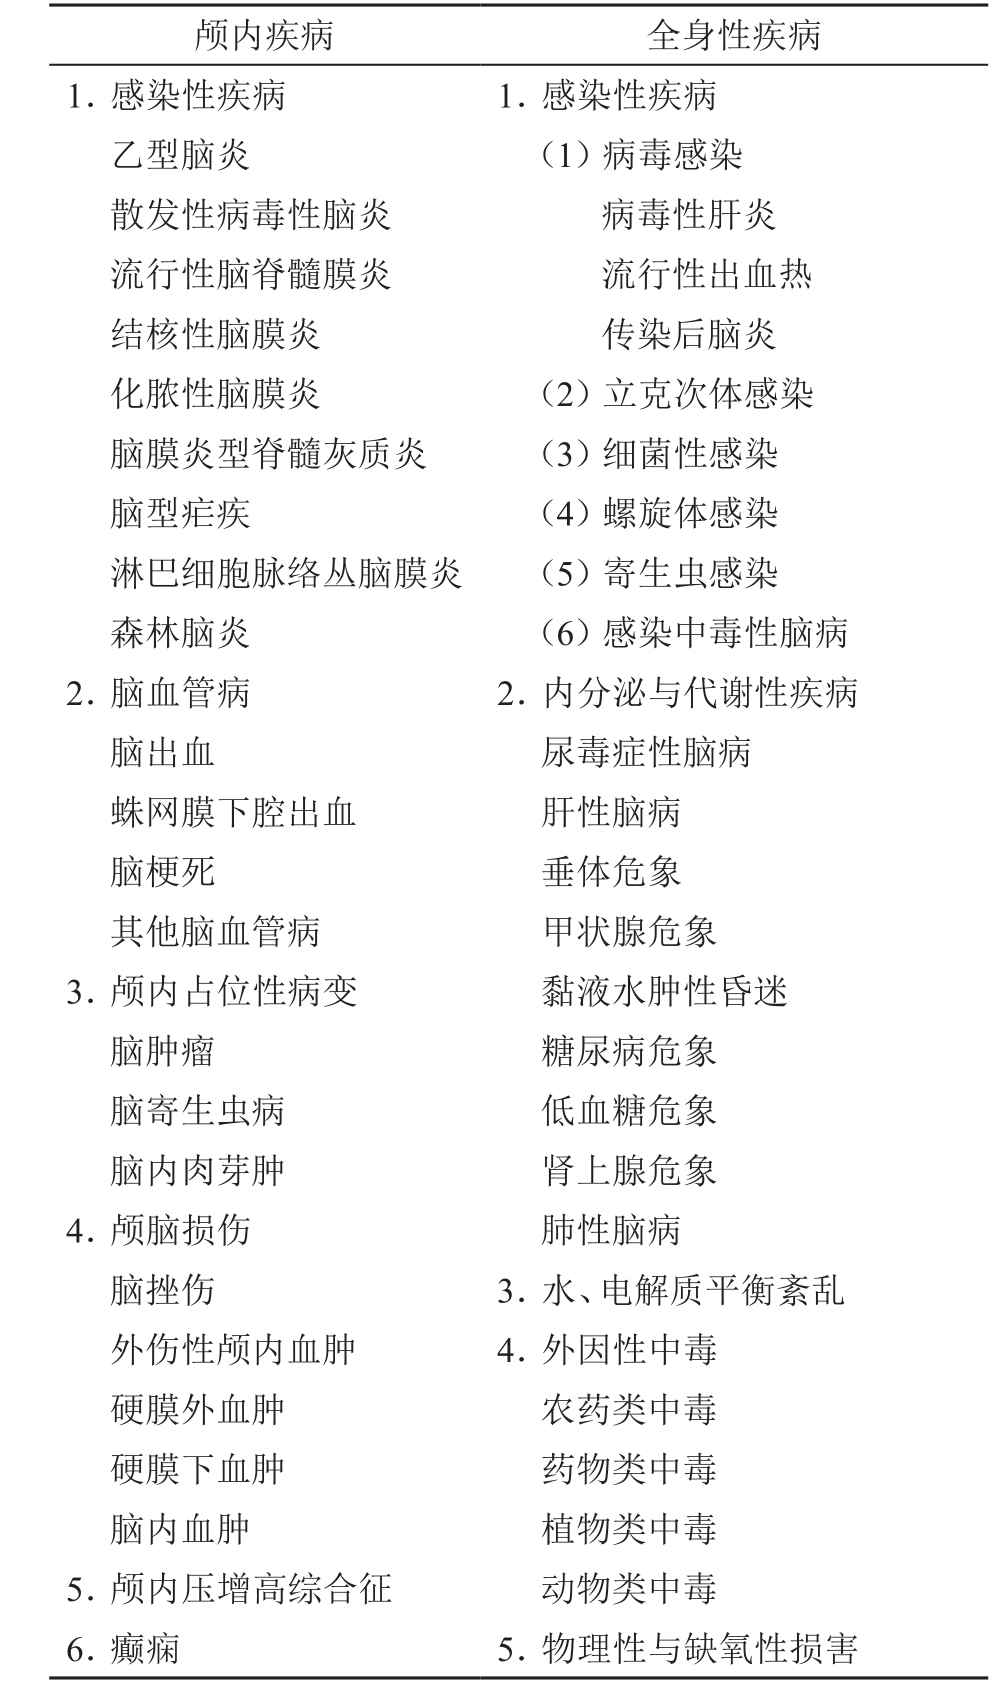
\includegraphics[width=3.3125in,height=5.67708in]{./images/Image00091.jpg}
\end{table}

临床上可依病因作用机制的不同分为直接损害和间接损害,前者指致病因素直接作用于脑组织(如锐器伤、火器伤及急性中枢性中毒等)立即引起脑功能衰竭者;后者指某种致病因素首先引起脑水肿及颅内压增高,再由颅内高压引起脑功能衰竭者。

被坚实颅骨保卫的人脑仅占体重的2\%,含有500亿以上的神经元和2500万亿以上的突触。脑细胞虽然不执行机械功或外分泌活动,但需要能量以合成细胞成分(据估计,每个细胞一天要生成2000个线粒体)和神经递质,经轴浆流运转细胞质,释放和摄取神经递质,逆电化学梯度或浓度梯度经细胞膜转运离子等。即使在“静止”状态,脑的代谢率也是非常高的。脑代谢的主要能量来源是葡萄糖。每100g脑组织1分钟约消耗5mg葡萄糖,成人脑每天要消耗120~130g葡萄糖作为能源。1mol葡萄糖酵解可提供2mol
ATP(三磷酸腺苷)的能量,而其经过三羧酸循环氧化后可产生36mol
ATP的能量。即:葡萄糖完全氧化后提供的能量为其乏氧代谢所产生能量的18倍。因此,葡萄糖的有氧氧化是供应脑能量的主要途径。静息状态下人脑的氧耗量占全身的20\%(5岁以下儿童占50\%)。脑组织内几乎没有氧的储存,产能底物------葡萄糖的含量也极少,远低于全身其他组织。脑组织完全依赖血液循环不断地供应产能底物和氧才得以维持其正常的结构和功能。人脑的血液供应相当于心排出量的15\%~20\%。脑循环具有自动调节的能力,脑内不同区域的脑血液随各该区域代谢率的变化而变化。在人体内,脑是对缺血缺氧最为敏感和最易受损的器官。在全脑缺血后1分钟内,脑内ATP含量降低90\%,以海马、大脑皮质、小脑Purkinje细胞和基底节为最敏感。正常静止状态下的平均脑血流量(CBF)每分钟为55ml/100g脑组织(灰质CBF约75ml/100g脑组织,白质CBF约30ml/100g脑组织)。当CBF降低至正常的35\%以下时(约每分钟15~20ml/100g脑组织)脑ATP储存耗竭,患者昏迷,脑电活动消失,但脑细胞仍保持存活。这是产生神经元电衰竭的血流阈值或称为功能损伤性缺血阈值。CBF降至正常的20\%或更低,则达(神经元)膜衰竭的血流阈值或称为形态损害性缺血阈值。在脑全面性缺血和局部缺血,总是有些神经死亡而有的神经细胞比较不易受损而仍保留功能。介乎这两类细胞之间的所谓“缺血半影区”(ischemic
penumbra),其神经细胞的功能丧失却依然存活。治疗努力的方向是使这些神经细胞的功能恢复而不发展至不可逆的阶段。

心脏骤停发生后大约15秒内随氧耗竭而意识丧失,紧接着葡萄糖和ATP也在4~5分钟内耗尽,脑干功能在1分钟后终止,呈临终呼吸,瞳孔散大、固定。一般认为,心脏骤停4~6分钟后发生不可逆的脑损害。脑血流中断是心脏骤停后脑损害的启动环节,而再灌注阶段血流动力学的紊乱延续和加重了脑缺血缺氧损害。再灌注紊乱大约经历4个时期,即无复流期、反应性充血期、延迟性低灌注期及后期改变。循环恢复早期由于脑微循环改变和脑灌注压低等原因可出现无复流现象,继而由于脑血管的麻痹出现数十分钟的反应性充血期,然后为延迟性多灶性低灌注期,此期可持续2~12小时,是脑缺血缺氧损害的最重要阶段。此后,局部CBF或改善而脑功能恢复,或继续恶化而细胞死亡。

目前尚无公认的心脏骤停后脑复苏不同时期的划分标准。一般来说,可分为三个时期:①脑损伤早期(心脏骤停后至自主循环恢复后12小时),此阶段为脑损伤启动环节,最重要的改变是循环和代谢异常,其中代谢异常是尤为关键的因素。②脑损伤中期(自主循环恢复后12~72小时),该段时间各种损伤级联反应发展至高峰并最终导致神经细胞死亡引起相应功能障碍。③脑损伤修复/恢复期(自主循环恢复72小时后)。

导致脑细胞损害的机制有以下学说:

\subparagraph{细胞内游离钙超载}

钙是最具生物活性的离子,神经细胞的许多生理活动,如神经递质释放、膜内外信息传递、膜兴奋的控制以及酶活性的调节等均有赖于钙的参与。游离的钙离子已被公认是细胞内的第二信使。细胞内游离Ca\textsuperscript{2+}
(Cai)的升降对调节细胞活动起决定性作用。为此,必须精确调控Cai,使之维持在一个相当恒定的水平上,以便对各种引起细胞内Ca\textsuperscript{2+}
上升的刺激作出敏感反应。正常情况下,膜内外存在极大的钙离子电化学梯度,细胞的调控机制使Cai维持在0.1~1μmol,而细胞外钙离子浓度(Cae)则高上万倍,约1.5mmol。这一离子梯度的维持除了细胞膜对Ca\textsuperscript{2+}
的相对不通透性外,主要依靠以下三个机制来完成:①胞浆蛋白的缓冲:胞内存在许多对Ca\textsuperscript{2+}
具有高度亲和力的蛋白,如钙调素(calmodulin)、Paralbumin等,主要在动作电位后约1~2毫秒内起作用,结合容量1~2μmol。②细胞器的封存:脑细胞内线粒体、光面内质网、突触小泡等都能摄Ca\textsuperscript{2+}
。细胞内最大的钙库位于线粒体,尤其当Cai >
1μmol时,线粒体摄Ca\textsuperscript{2+}
明显增加;Cai超过5μmol时,大多数Ca\textsuperscript{2+}
被线粒体封存;而当Cai <
0.4~0.5μmol时,线粒体几乎不贮Ca\textsuperscript{2+}
。这提示线粒体摄取Ca\textsuperscript{2+}
仅发生在Cai大量增加时。③细胞质膜上的Ca\textsuperscript{2+}
运转:钙泵(Ca\textsuperscript{2+} -Mg\textsuperscript{2+}
-ATP酶)能主动运输Ca\textsuperscript{2+}
进入光面内质网或泵出胞外,但效率较低。膜Na\textsuperscript{+}
/Ca\textsuperscript{2+}
交换系统作用较大,能利用膜内外Na\textsuperscript{+}
梯度,在Na\textsuperscript{+} 进入细胞的同时,将Ca\textsuperscript{2+}
带出胞外。由于膜内外Na\textsuperscript{+}
梯度约1∶10,而Ca\textsuperscript{2+} 梯度高达1∶10
000,有学者推测可能需要进入3~4个Na\textsuperscript{+}
才能带出1个Ca\textsuperscript{2+} 。可见,Ca\textsuperscript{2+}
外流是“骑跨”在Na\textsuperscript{+} 梯度上的,若Na\textsuperscript{+}
梯度消失则Ca\textsuperscript{2+}
外流停止。各种疾病造成细胞内钙超载、钙离子内环境失稳是导致细胞死亡的“最后共同途径”。CBF降至正常的20\%以下时,细胞产能过程破坏而致细胞膜离子泵停止运转。细胞外钾离子浓度增高触发钙离子内流,同时胞内钙库释放封存的钙离子,导致细胞内游离钙超载,细胞内高浓度的钙可通过直接作用和各种钙相关酶的激活而引起细胞器损伤、蛋白质降解和DNA断裂,加速神经细胞凋亡(apoptosis)和坏死。过多的Ca\textsuperscript{2+}
激活许多钙敏感酶,如核酸内切酶、蛋白酶、一氧化氮合酶,后者将左旋精氨酸转为左旋瓜氨酸时产生一氧化氮,其具有自由基性质;钙超载使线粒体功能发生障碍,氧化磷酸化电子传递脱耦联,ATP产生大量减少并在原位消耗,造成反应氧中间产物的增加。一氧化氮自由基和反应氧的中间产物均具损害性,两者结合导致DNA碎裂。在钙离子内流介导的一系列反应中,通过严重耗尽细胞内能量而间接导致细胞死亡;某些状态下,一氧化氮也激活肿瘤抑制基因P53,最终能导致细胞凋亡。此外,细胞内钙超载介导NMDA受体过度刺激致细胞凋亡。

\subparagraph{自由基的生成与毒性反应}

自由基是游离存在的、带有不成对电子的分子、原子或离子,其化学性质活泼,易与其他分子发生反应。脑缺血时生物氧化呼吸链传递过程发生自动氧化,使氧还原成超氧阴离子自由基。缺血时ATP的降解过程在黄嘌呤氧化酶的作用下,在次黄嘌呤氧化过程也生成超氧阴离子。脑缺血后自由基的另一来源与前列腺素合成有关。缺血损伤后磷脂酶被激活,引起膜磷脂的降解,产生大量花生四烯酸,在环氧合酶的作用下合成前列腺素的过程中,有超氧阴离子等自由基生成。此外,脑缺血后脑内清除自由基能力下降,进一步加重了自由基的损伤作用。自由基具有广泛的细胞损伤活性:过氧化不饱和脂肪酸,破坏细胞膜的屏障作用;损伤线粒体膜,加重细胞能量代谢障碍;破坏酶和蛋白质,导致细胞功能和结构破坏;引起DNA断裂以及细胞变性、坏死。

自由基损伤往往在缺血后再灌注时更为突出。血流再通时,氧的供给很快得到恢复,但体内三羧酸循环恢复较慢,不能提供足够的电子将氧还原为水,而形成超氧阴离子。缺血时ATP分解生成大量次黄嘌呤,再灌注时氧可以加速黄嘌呤氧化酶催化反应,使次黄嘌呤转变为黄嘌呤,同时生成较多的超氧阴离子自由基。

\subparagraph{兴奋性氨基酸}

(EAA)的神经毒性作用
谷氨酸(Glu)和天冬氨酸(Asp)是中枢神经系统的兴奋性递质,又称兴奋性氨基酸(EAA)。正常情况下,神经末梢释放的Glu、Asp绝大部分经神经末梢再摄取,此过程耗费能量。当脑组织能量代谢受缺血缺氧等损害后,EAA的再摄取下降;神经细胞内钙超载又促使EAA的过量释放。EAA对兴奋性氨基酸受体的持久性刺激可引起神经元的损害和死亡。大量EAA作用于EAA受体------主要是NMDA(N-甲基-D-天冬氨酸)受体,打开了Ca\textsuperscript{2+}
和Na\textsuperscript{+} 通道,促使Ca\textsuperscript{2+}
、Na\textsuperscript{+} 内流,K\textsuperscript{+}
外流,造成神经细胞内外离子平衡紊乱,导致细胞内Ca\textsuperscript{2+}
超载,细胞内水肿,神经细胞肿胀、坏死。

\subparagraph{膜磷脂代谢障碍}

Cai剧增和自由基引起的过氧化反应均激活细胞质膜的磷酸脂而产生大量FFA。花生四烯酸(AA)本身破坏血脑屏障(BBB),具强力的致脑水肿作用。AA在环氧合酶作用下产生的TXA\textsubscript{2}
和在脂氧合酶作用下产生的白三烯(LT)具有血管收缩的作用,促进脑血管痉挛、血小板凝聚及微血栓形成、微循环障碍,使周围脑组织血供恶化,脑水肿加重,且LT可使BBB破坏,加重脑水肿。脑缺血时,脑组织内的TXA\textsubscript{2}
和LT增高并随缺血时间延长而增加。因此,缺血时间愈长,脑损害愈重。

\subparagraph{乳酸性酸中毒}

正常情况下,脑细胞通过葡萄糖的有氧氧化代谢而获得能量。脑血流的突然中断使氧化磷酸化反应立即停止。内源储存的葡萄糖和糖原还足以使无氧糖酵解维持一段时间,结果使细胞内乳酸大量积聚而发生乳酸性酸中毒。细胞外Na\textsuperscript{+}
与细胞内H\textsuperscript{+}
交换而进入细胞内产生脑水肿。此时给严重缺血、缺氧的脑组织继续提供葡萄糖只能加重酸中毒的程度和脑损害。

\subparagraph{分子水平机制}

已有的研究表明脑缺血缺氧损伤时,神经细胞有多种基因表达异常,如即早期基因c-fos、c-jun以及热休克蛋白等表达明显增加,而微管相关蛋白、微管运动蛋白等细胞结构蛋白表达则下降,基因以及相应的功能蛋白的表达改变可能是脑缺血性损害的分子基础。近来研究发现,心肺复苏术(CPR)后3小时,丘脑等缺血易损伤区域凋亡相关配体Fasl表达明显上调,可能是这些区域易于发生缺血性损伤的原因之一。

\subparagraph{其他机制}

包括激肽释放酶-激肽原-激肽系统的致脑水肿作用、溶酶体膜破坏和内源性阿片样物质(β-内啡肽、强啡肽)的有害作用等。

上述各种脑细胞损害的机制,均可引起脑水肿。脑水肿是脑组织对各种致病因素的一种反应,主要变化为脑实质内液体成分的增加,引起脑体积的增大。一般把脑水肿分为以下三种类型:

1.细胞毒性脑水肿
多见于脑缺血缺氧早期以及脑膜炎等疾病。主要表现是脑细胞(神经元、胶质细胞)因细胞内液增多而肿胀,即细胞水肿。无血管损伤,血脑屏障相对完整,血管通透性无损害。引起水肿的机制可能是因缺血、缺氧或在某些毒性物质的作用下,细胞Na\textsuperscript{+}
泵功能受损,致细胞内Na\textsuperscript{+}
潴留,细胞内水亦增多。此型脑水肿意识障碍较常见,轻者嗜睡,重者昏迷。脑电图检查多为弥漫性高波幅慢波。

2.血管源性脑水肿
多见于脑缺血缺氧严重时,以及脑肿瘤、脑外伤等疾病时。主要表现是灰质胶质细胞肿胀、水肿,而白质中除胶质细胞水肿外,细胞外间隙有液体积聚,其水肿液含较多蛋白质。其机制是由于毛细血管通透性增高,血脑屏障破坏,引起血浆中水与其他分子外渗的结果。此型脑水肿严重时常有明显的颅内压增高,并出现意识障碍。

3.间质性脑水肿
见于肿瘤以及炎症性疾病。其主要表现是脑室周围间质中出现水肿,因炎症等可使脑脊液生成增加,或是因肿瘤等压迫、阻塞脑脊液循环通路,故可影响脑脊液正常循环而出现脑室扩张,形成脑积水。脑积水时,脑脊液压力增高,同时还可因炎症等的影响,室管膜的通透性增高,故脑脊液可渗入脑室周围的白质细胞间隙中,呈间质性水肿。此型脑水肿大脑功能改变较缓慢,一般无意识障碍,脑电图常为正常。

脑水肿的病理形态,可分为局灶性脑水肿和弥漫性脑水肿两类。如脑水肿较局限或程度较轻时,临床上可不出现,或仅出现轻微的脑功能异常,亦可不出现意识障碍;只有局灶性大脑占位病变引起严重脑水肿发生脑疝时,才可出现意识障碍。另一种弥漫性脑水肿,常为严重颅脑外伤、颅内感染、中毒及缺氧等病因引起,常见有局限性神经功能障碍及颅内压增高征,重者脑疝形成,多见有意识障碍。

引起脑功能衰竭的各种病因,它们或是直接致颅内容物体积增加,或是致脑脊液循环障碍,或是引起脑水肿,导致颅内压增高及意识障碍;而脑水肿则是致颅内压增高的主要原因。从临床病理生理学角度,可将颅内压增高的发生发展分为代偿期、早期、高峰期和晚期等四个不同阶段(参见第41章“颅高压危象”部分)。当颅内压升高到颅内无法缓冲时,某些脑组织受挤压,并向邻近阻力最小的空间疝出(脑疝形成)。不仅疝出的脑组织发生淤血、水肿和软化,受疝组织挤压的四邻结构也将发生一系列神经功能障碍;同时疝组织阻塞脑脊液循环通路,导致颅内压更为增高。周而复始和恶性循环,最后致急性脑功能衰竭和一系列危急临床症状。

\subsection{诊断}

急性脑功能衰竭常是许多颅内疾病和全身性疾病的严重后果,如何在各种疾病的发生发展中确定已发生脑功能衰竭,是一个十分紧迫的问题。因其对早期防治脑功能衰竭,改善预后有重要意义。在脑功能衰竭的诊断上,必须包括临床诊断、脑损害部位和病因诊断以及脑死亡的确定。

\subsubsection{临床诊断}

脑功能衰竭时,脑内发生一系列生理生化改变,临床上出现许多症状和体征,而实验室检查所见则是非特异性的,主要是与原发病有关的变化。因此,脑功能衰竭的诊断主要是依据脑部受损的临床征象。不论病因如何,临床诊断主要包括意识障碍和颅内压增高的分析和判断。

\hypertarget{text00067.htmlux5cux23CHP3-1-2-1-1}{}
(一) 意识障碍

意识障碍是急性脑功能衰竭的主要临床表现之一。意识正常即意识清醒,表现为对自身与周围环境有正确理解,对内外环境的刺激有正确反应,对问话的注意力、理解程度以及定向力和计算能力都是正常的。意识障碍通常可分为觉醒障碍和意识内容障碍。依据检查时刺激的强度和患者的反应,可将觉醒障碍区分为嗜睡、昏睡、浅昏迷、中昏迷和深昏迷;意识内容障碍常见的有意识模糊、精神错乱、谵妄状态。有关意识障碍的判断及鉴别诊断,详见本书第2章“意识障碍和昏迷”部分。

\hypertarget{text00067.htmlux5cux23CHP3-1-2-1-2}{}
(二) 脑水肿、脑疝

脑功能衰竭的重要病理改变是脑水肿、颅内压增高。典型表现为头痛、恶心呕吐与视神经乳头水肿,常伴有血压增高、脉搏缓慢、呼吸慢而深、瞳孔缩小、烦躁不安或意识障碍、抽搐等生命体征的变化。随着颅内压增高,终致脑疝形成。急性发作者常表现为突然和急剧进展的意识障碍,瞳孔变化,呼吸与循环功能异常,肌张力障碍等。如未及时解除,可在短时间内致死。脑疝的出现是急性脑功能衰竭发生发展的严重后果,早期识别与防治它的形成与发展有极其重要的意义。临床上常见而危害大的脑疝有小脑幕裂孔下疝,枕骨大孔疝和小脑幕裂孔上疝,它们可单独存在或合并发生。

\subparagraph{小脑幕裂孔下疝}

为部分颞叶和(或)脑中线结构经小脑幕裂孔往下疝出的一种脑疝。脑疝形成后使脑池闭塞,颅内压更增高,脑干被迫下移,位于中脑大脑脚与小脑幕切迹缘间的动眼神经,常因早期受压麻痹而出现同侧上睑下垂、瞳孔散大与眼球外展,继而大脑脚受压,对侧肢体瘫痪;随着移位的增加对侧大脑脚被压于小脑幕的游离缘上引起病侧肢体瘫痪,对侧的动眼神经亦可受牵拉或压迫而形成双侧瞳孔散大,且散大较病变侧明显,眼球运动麻痹。因此,临床上如怀疑有外伤性急性颅内血肿存在,而按瞳孔散大侧施行颅钻孔探查时,如为阴性,尚需作对侧钻孔探查,以免遗漏血肿。当中脑网状结构上行激活系统受损时,可出现不同程度的意识障碍或昏迷,并逐渐加深。脑疝的继续发展,使脑干受压损害逐渐加重,出现四肢肌张力增高、瘫痪,并有强直样发作,称为去大脑强直。生命指征的改变随脑疝的发生发展而变化:①脑疝前期:脑疝时引起脑干缺氧,而脑干对缺氧耐受性较强;早期缺氧对脑干生命中枢起兴奋作用,从而出现呼吸深快,脉搏加快,血压升高;当颅内压继续升高时脉搏变慢。②脑疝代偿期:当脑干受压、脑缺氧与脑水肿更为严重时,生命中枢还可以暂时通过生理调节来维持生命活动,于是呼吸、循环中枢兴奋加强,克服缺氧,因而血压更趋升高,脉搏缓慢(50次/分以下),呼吸深而节律不整。③脑疝晚期:呼吸与循环中枢处于衰竭状态,出现呼吸变浅而不规则,甚至呼吸停止、血压下降、心律失常、心跳停止。

\subparagraph{枕骨大孔疝}

枕骨大孔为颅后凹与椎管间交通孔道,孔之前半部有延髓,后半部有小脑延髓池(又称枕大池),小脑扁桃体居小脑半球后下部,紧邻枕骨大孔上缘。当颅内压增高时,小脑受挤促使小脑扁桃体向下移位和嵌入上颈段椎管内(称枕骨大孔疝或小脑扁桃体疝),使小脑延髓池闭塞,脑脊液循环受阻,颅内压进一步增高,小脑扁桃体进一步下移和紧紧地嵌入枕骨大孔和颈椎椎管上端,损及延髓及其邻近的第9~12对脑神经和第1~2对脊神经根、小脑后下动脉等重要结构,颅内压更加增高,如此恶性循环,最后像小脑幕裂孔下疝一样的结局都可发生。不同的是,枕骨大孔疝的呼吸、循环中枢功能障碍出现较早,瞳孔和意识障碍出现较晚,而小脑幕裂孔下疝恰好相反。

枕骨大孔疝多见于颅后凹占位性病变,亦见于引起严重脑水肿的颅内弥漫性病变。幕上占位性病变先形成小脑幕裂孔下疝,最后常合并有不同程度的枕骨大孔疝。可分为急性和慢性两型,后者常由慢性颅内压增高或颅后凹占位病变引起,临床上除有枕后部疼痛(因颈神经根受激惹)、颈项强直与压痛,第9~12对脑神经受损(如轻度吞咽困难、饮食呛咳与听力减退)外,偶有四肢强直,角弓反张甚或呼吸抑制,但意识常清楚,可能与机体已具有一定代偿功能有关,然晚期仍无例外地出现意识障碍。急性型多系突然发生,或在慢性型的基础上,因剧烈呕吐、咳嗽、挣扎、排便用力、腰穿或作压颈试验等促使颅内压增高的因素突使加剧,常可突然发生呼吸停止、昏迷而死亡。

\subparagraph{小脑幕裂孔上疝}

是由于幕下颅内压增高使脑组织经小脑幕裂孔向上疝出所致。疝内容物主要是小脑上蚓部与小脑前叶,故又称小脑蚓部疝。多为颅后凹病变引起,常与枕骨大孔疝合并发生。颅后凹占位性病变病例作侧脑室快速引流时可诱发或加重此疝。当上述疝组织疝入四叠体池和压迫中脑后部的四叠体及被盖部时,可早期出现上睑下垂、双眼上视困难、瞳孔散大、对光反射消失和听力障碍等四叠体受损症状,以及被盖部内网状结构上行激活系统受损所致的意识障碍;晚期有去大脑强直与呼吸骤停。

\subsubsection{脑功能障碍解剖部位判断}

急性脑功能衰竭时,脑内发生一系列的病理过程,可损害不同部位的结构及功能,呈现各种临床征象。临床上分析脑受损的部位及其功能障碍水平是非常重要的,对指导治疗、判断预后有较大价值。通常可根据意识状态、颅内压增高征、脑损害的症状和体征,结合必要的辅助检查,来推断脑部损害的范围及功能障碍水平。一般分为以下三种情况:

\hypertarget{text00067.htmlux5cux23CHP3-1-2-2-1}{}
(一) 幕上局限性病变

大多先有大脑半球损害的征象
,常有定位表现,如癫痫、轻偏瘫、偏盲、失语等,迟早可出现颅内压增高的征象。当病变位于“静区”,如额叶或硬脑膜下间隙,可无局灶征,仅呈弥散性脑功能障碍和颅内高压症。随着病程进展,当病变累及间脑中央部,则发生意识障碍,继而进一步发展为小脑幕裂孔下疝,出现自上而下的脑干受损征象。因此,幕上病变的病程规律,一般是大脑半球损害的对侧定位征和颅内压增高征,其后依次出现意识障碍和脑干受损的表现。

\hypertarget{text00067.htmlux5cux23CHP3-1-2-2-2}{}
(二) 幕下局限性病变

主要特点是脑干功能障碍
,一般在发生意识障碍的同时,常已伴随同水平脑干受损征象。因此,患者在昏迷前无大脑半球的偏侧定位体征,而常有枕区疼痛、恶心、呕吐、眩晕发作、复视、眼球震颤、共济失调、一侧脑干局限体征(如交叉性瘫痪)、后组脑神经麻痹等。若尚未影响脑脊液循环,则无颅内压增高的征象或较晚出现,但颅后凹占位性病变可较早发生颅内高压征,且较易引起枕骨大孔疝,通常不发生幕上病变那种自大脑皮质、间脑至脑干的病程规律。

\hypertarget{text00067.htmlux5cux23CHP3-1-2-2-3}{}
(三) 弥散性脑损害

急性的大脑弥散性损害,由于大脑皮质及皮质下结构受损,临床上常先有精神症状,意识内容减少,一般呈现对外界的注意力降低,计算与判断力辨别差,记忆障碍和定向力障碍,错觉、幻觉、谵语。很快出现较明显的觉醒障碍,呈现嗜睡或昏睡,直至昏迷,其程度常同病变的范围和严重程度相应。也常发生去大脑皮质状态。大多缺乏明确的脑局灶性定位征,而呈弥散性或多灶性损害的体征,常伴颅内高压征和脑膜刺激征;晚期可呈现继发性脑干功能障碍的征象。

各阶段脑功能障碍的特征见表\ref{tab25-2}。

\subsubsection{病因诊断}

脑功能衰竭的病因诊断极为重要。通常必须依据病史、体格和神经系统检查,以及有关的实验室资料,经过综合分析,能查出导致脑功能障碍的原发病因。由于脑功能衰竭的病因众多,而且某些病例的病程进展甚快,病情危重或因条件所限,无法进行详细或特殊的实验室检查,使病因诊断受到影响。从临床实际需要出发,区分原发病变位于颅内或颅外,具有较大价值。

\begin{table}[htbp]
\centering
\caption{各阶段脑功能障碍的特征}
\label{tab25-2}
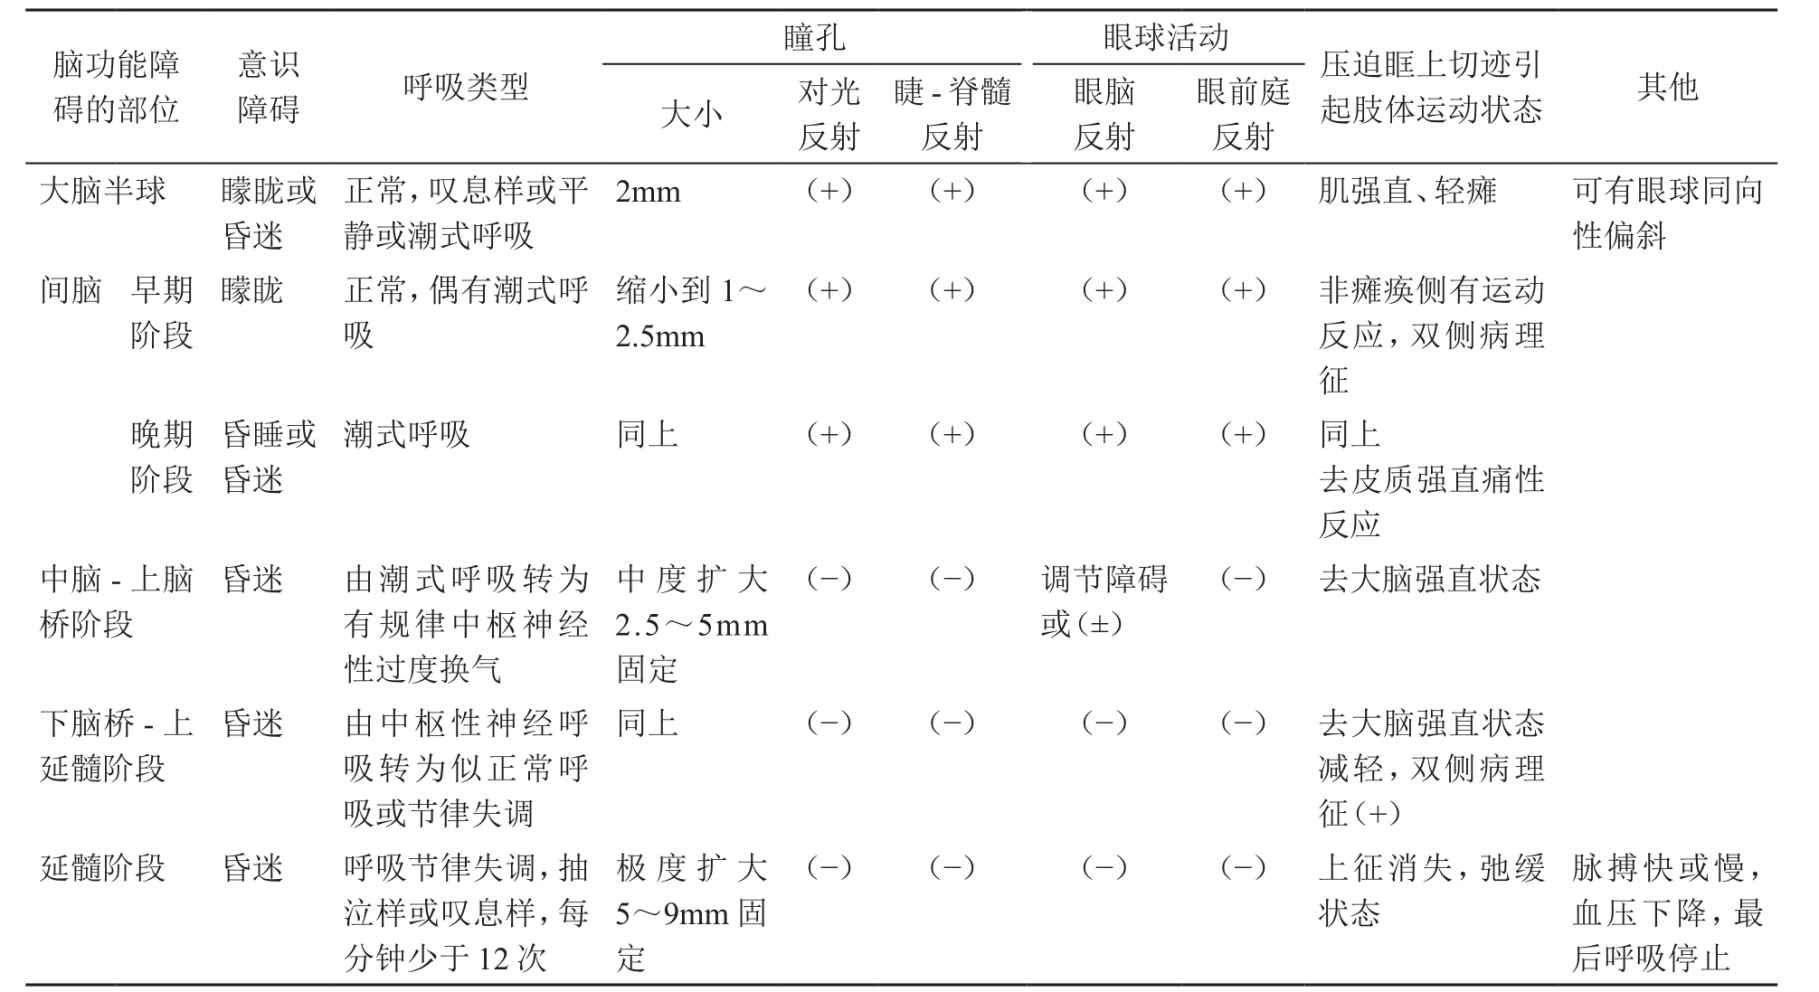
\includegraphics[width=6.69792in,height=3.64583in]{./images/Image00092.jpg}
\end{table}

\hypertarget{text00067.htmlux5cux23CHP3-1-2-3-1}{}
(一) 颅内疾病

原发病变在颅内
,随着病程进展,最终导致脑功能衰竭。临床上通常先有大脑或脑干受损的定位症状和体征,较早出现意识障碍和精神症状,大多伴明显的颅内压增高,有关颅内病变的辅助检查多有阳性发现。常见的有急性脑血管病、颅内占位性病变(肿瘤、脓肿)、颅脑损伤、颅内感染以及癫痫持续状态等。

\hypertarget{text00067.htmlux5cux23CHP3-1-2-3-2}{}
(二) 全身性疾病

全身性(包括许多内脏器官)疾病可影响脑代谢而引起弥散性损害,又称继发性代谢性脑病。同原发性颅内病变相比,其临床特点是:先有颅外器官原发病的症状和体征,以及相应的辅助检查的阳性发现,后才出现脑部受损的征象。由于脑部损害为非特异性或仅是弥散性功能抑制,临床上一般无持久和明显的局限性神经体征及脑膜刺激征,主要是多灶性神经功能缺失的症状和体征,且大都较对称。通常先有精神异常、意识内容减少。一般是注意力减退、记忆和定向障碍,计算和判断力降低,尚有错觉、幻觉,随病程进展,意识障碍加深。此后有的可出现不同层次结构损害的神经体征,如昏迷较深和代谢性抑制很严重,而眼球运动和瞳孔受累却相对较轻。常见病因有外源性中毒、内分泌与代谢性疾病、感染性疾病、物理性与缺氧性损害等。

\subsubsection{脑功能监测}

脑功能监测是为了解中枢神经功能损害的程度及抢救治疗的效果。

\hypertarget{text00067.htmlux5cux23CHP3-1-2-4-1}{}
(一) 必要的神经系统检查

1.角膜反射
是衡量意识障碍程度的重要标志。长时间的角膜反射消失,常提示预后不良。

2.其他反射
瞳孔对光反射、咳嗽、吞咽反射、脊髓反射等的存在或消失,提示脑干功能恢复或消失。

3.瞳孔大小的变化。

\hypertarget{text00067.htmlux5cux23CHP3-1-2-4-2}{}
(二) 电生理监测

\subparagraph{脑电图}

须连续监测,对脑功能状态、病变部位、治疗及预后判断都有一定价值。脑电图正常,预后良好,可以完全恢复脑功能;脑电图极度异常,提示中枢神经功能严重受损。

\subparagraph{脑干诱发电位}

为测定脑干功能状态的客观方法。常用的为脑干听觉诱发电位,因其一般不受麻醉药物的影响。

\subparagraph{颅内压监测}

采用各种小型颅内压计,埋藏在颅内,连续记录颅内压,能较好的反映脑水肿的情况。

\subsubsection{脑死亡的确定}

脑功能衰竭的最严重后果是脑功能的永远不能恢复,称为脑死亡或过度昏迷或不可逆性昏迷。系指枕骨大孔以上(包括第一颈髓)颅腔内全部脑神经元的不可逆性死亡。脑死亡是颅内结构的最严重损伤,一旦发生,即意味着生命的终止。

\hypertarget{text00067.htmlux5cux23CHP3-1-2-5-1}{}
(一) 成人脑死亡的诊断标准

2009年卫生部脑死亡判定标准起草小组提出的脑死亡判定标准(成人)(修订稿)如下:

\subparagraph{判定的先决条件}

①昏迷原因明确;②排除了各种原因的可逆性昏迷。

\subparagraph{临床判定}

①深昏迷;②脑干反射消失;③无自主呼吸(靠呼吸机维持,自主呼吸激发试验证实无自主呼吸)。

以上三项必须全部具备。

\subparagraph{确认试验}

①正中神经短潜伏期体感诱发电位(SLSEP)显示N9和(或)N13存在,P14、N18和N20消失;②脑电图(EEG)显示电静息;③经颅多普勒超声(TCD)显示颅内前循环和后循环呈振荡波、尖小收缩波或血流信号消失。

以上三项中至少两项阳性。

\subparagraph{判定时间}

临床判定和确认试验结果均符合脑死亡判定标准者可首次判定为脑死亡。首次判定12小时后再次复查,结果仍符合脑死亡判定标准者,方可最终确认为脑死亡。

\hypertarget{text00067.htmlux5cux23CHP3-1-2-5-2}{}
(二) 小儿脑死亡的诊断标准

由于 5岁以下儿童脑的可塑性大
,脑的发育尚未成熟,对脑损伤的耐力较成人为大,故上述成人的脑死亡标准并不完全适宜于儿童。

\subparagraph{美国儿童脑死亡判断特别工作组拟定的标准(1987年)}

\hypertarget{text00067.htmlux5cux23CHP3-1-2-5-2-1-1}{}
(1) 临床标准:

①昏迷和呼吸停止,完全失去知觉,无意识活动;②脑干功能丧失:瞳孔扩大、固定,对光反射消失;自发眼活动消失,眼-头和眼前庭反射消失;延髓肌肉系统的运动消失,包括面部及口咽肌肉,角膜、咽、咳嗽、吸吮等反射均消失;脱离呼吸机则病儿无自主呼吸运动,可采用标准方法进行呼吸暂停试验,但需有其他标准存在时才做。③无低温和低血压。④肌张力弛缓,自发活动或诱发活动消失。但需排除脊髓反射如缩回反射或脊髓肌痉挛反射的存在。⑤在观察期应反复检查。

\hypertarget{text00067.htmlux5cux23CHP3-1-2-5-2-1-2}{}
(2) 观察期(按年龄大小而定):

不到7天生命的婴儿不用脑死亡这一诊断。①7天~2个月:两次检查间隔至少48小时(包括脑电图)。②2个月~1岁:两次检查间隔至少24小时。若脑血管造影证实颅内无血管显像,就不必再继续检查。③1~5岁的儿童:两次检查间隔至少12小时。对年长儿童,参照成人标准。

凡已肯定为不可逆的病情时,可不必再进行实验室检查,观察期至少12小时。若为缺血-缺氧性脑病,难确定脑损害的可逆性及其范围,可将观察期延至24小时。当脑电图平坦或脑血管造影无颅内血管显影时,观察期可以缩短。

\hypertarget{text00067.htmlux5cux23CHP3-1-2-5-2-1-3}{}
(3) 实验室检查:

①脑电图:描记至少30分钟,脑波为平线。②脑血管造影:示脑循环停止即可诊断为脑死亡。③颈内动、静脉氧差:在脑死亡患者,几乎无差别。④阿托品试验阴性。⑤脑干听觉诱发电位(BAEP):各波均消失或仅1波残存,潜伏期延长。⑥TCD检查:多为无信号。⑦前庭变温试验:无眼震出现。

\subparagraph{中国儿童脑死亡诊断标准试用草案}

(1989年)①持续深昏迷,无自主运动,对外界刺激无反应;②经反复停机试验证实无自主呼吸;③瞳孔扩大、固定,光反射、角膜反射消失;④心率固定,对刺激无反应,包括静脉注射阿托品;⑤排除低温、麻醉剂、肌肉松弛剂、大剂量镇静剂、严重代谢和内分泌紊乱等所致假象。

\subsection{治疗}

急性脑功能衰竭是多种病因和不同性质病变所致的一种临床病理状态,并常引起许多严重并发症,因此必须根据不同的病因与病理阶段,采取最佳的综合治疗方案,以控制或逆转脑功能衰竭的发展,解除或最大限度地减轻脑损害,争取恢复正常的功能。

\subsubsection{一般处理}

原则上应将患者安置在有抢救设备的重症监护室内,以便于严密观察,抢救治疗。给氧,加强护理。一般常取侧卧位或仰卧位(头偏向一侧),利于口鼻分泌物的引流。保持床褥平整、清洁,一般每2~4小时翻身1次,骨突易受压处加用气圈或海绵垫,并适当按摩。防止舌后坠,定期吸痰,保持呼吸道通畅,注意口腔清洁。留置尿管者,定期冲洗膀胱及更换尿管。急性期有昏迷者先短时禁食,靠静脉补液,在生命体征稳定后,依病情给予易消化、高蛋白、富维生素、有一定热量的流质(可行鼻饲)。

\subsubsection{病因治疗}

针对病因采取及时果断措施是抢救脑功能衰竭的关键。对病因已明确者,则迅速给予有效的病因处理。如颅脑外伤与颅内占位性病变,应尽可能早期手术处理;出血性脑血管病有指征时尽早行手术清除血肿,或行脑室穿刺引流术;急性中毒者应及时争取有效清除毒物和特殊解毒措施的应用;各种病原体引起的全身性感染和(或)颅内感染,应选用足量敏感的抗生素等药物。

\subsubsection{对症处理}

\subparagraph{控制脑水肿 ,降低颅内压}

除采取保持呼吸道通畅、合理的维持血压、适量的补液及防止高碳酸血症等措施外,尚需用脱水剂。如20\%甘露醇液125~250ml静脉快速滴注,依病情每4~12小时1次;呋塞米(速尿)20~40mg或依他尼酸(利尿酸钠)50~100mg静注,50\%葡萄糖液40~100ml静注,每4~12小时1次;地塞米松10~40mg/d静滴;20\%人体白蛋白50~100ml/d静滴;常用上述药物联合或交替使用。

\subparagraph{维持水、电解质和酸碱平衡}

一般每日静脉补液量1500~2000ml,其中5\%葡萄糖盐水500ml左右;同时应注意纠正电解质紊乱如低钾或高钾血症,以及酸碱平衡失调。

\subparagraph{镇静止痉}

对有抽搐、兴奋躁动等表现者,可选用地西泮(安定)、苯巴比妥、苯妥英钠等镇静、抗惊厥药物,亦可用东莨菪碱0.3~0.6mg肌注,或异丙嗪(非那根)25~50mg肌注,对高热伴抽搐者可用人工冬眠疗法。

\subparagraph{控制感染}

有感染者,应根据细菌培养与药敏结果选择有效的抗生素。

\subparagraph{防治脏器功能衰竭}

包括防治心、呼吸和肾功能衰竭,以及消化道出血等并发症。参见有关章节。

\subsubsection{低温疗法}

轻度低温(体温32~34℃)治疗是目前唯一在临床研究中证实有效的脑保护措施,应作为脑功能衰竭的常规治疗措施。其脑保护作用可能与以下因素有关:①减少兴奋性氨基酸释放;②抑制一氧化氮(NO)合酶的激活,减少NO的产生;③降低组织氧耗,延缓继发性脑能量代谢障碍的发生,减少ATP消耗和防止细胞膜去极化;④抑制细胞内钙超载的发生;⑤改善脑血流紊乱和减轻脑水肿;⑥减轻细胞内酸中毒;⑦减弱自由基反应,保护脑组织自身抗氧化能力;⑧抑制蛋白激酶C的活性,减轻Ca\textsuperscript{2+}
介导的神经损伤作用;⑨减轻缺血导致的微管相关蛋白的丧失,维持正常的神经元细胞骨架。

低温疗法一般采用全身降温和头部局部降温(降温头盔、降温颈圈等)。全身降温效果较确切,包括降温毯或降温仪、胃内注入冰水、腹腔灌洗和体外泵等。常用的降温措施是使用降温毯放置在患者身体的上、下面和冰盐水鼻胃灌洗。一旦直肠温度达到33℃,通过降温毯恒温器的调整,保持患者的体温在32~34℃。由于32℃以下低温在临床上可带来许多严重并发症如诱发室颤等,应尽量避免温度低于32℃。在采用低温疗法时,为防止患者寒战,需要给予镇静药物,首选异丙酚{[}剂量宜≤50μg/(kg•min){]},必要时需持续静脉滴注神经肌肉阻滞剂维库溴铵和麻醉剂芬太尼等。在降温期间,加强心电、SaO\textsubscript{2}
、血压和呼吸监测,使MAP维持在90~110mmHg。有条件时可使用带有能够测量脑部温度的微热敏电阻式颅内传感器。低温疗法应用时间取决于患者的病情,一般可采用2~14天。复温要慢,速度过快对颅内压增高者非常有害,应该用10~12小时以上时间逐渐完成(<
0.5℃/h)。低温疗法时应注意防治以下并发症:①心律失常;②出血倾向;③肺部感染;④水、电解质紊乱,低温时低钾和高温时高钾;⑤低温期休克和复温时颅内压增高等。一般认为,对脑功能衰竭患者伴休克状态、用升压药物维持血压者和临床已有脑死亡征象者,不宜采用低温疗法。

\subsubsection{脑保护剂的应用}

某些药物能减少或抑制自由基的过氧化作用,降低脑代谢从而阻止细胞发生不可逆性改变,形成对脑组织的保护作用,称为脑保护剂。如巴比妥类、苯妥英钠、甘露醇、纳洛酮(naloxone)和钙拮抗剂等。近年来神经节苷脂、氧自由基清除剂、凋亡抑制剂、干细胞移植、腺苷及其类似物、兴奋性氨基酸受体拮抗剂、谷氨酸释放抑制剂、谷氨酸转运蛋白调节剂、缓激肽受体拮抗剂、热休克蛋白、镁离子等对脑损伤的治疗保护作用亦受到临床重视。但几乎所有的脑保护剂都有一个共同的结果,即动物实验有效,而临床无效或效果可疑。

\subparagraph{纳洛酮}

系阿片受体拮抗剂,能有效地拮抗β-内啡肽(β-EP)对机体产生的不良反应,具有明显的脑保护作用。其作用机制是:①抑制缺血时细胞膜脂质分解代谢,抑制氧自由基的产生和抗脂质过氧化作用,增加细胞膜的稳定性;②改善缺血时神经细胞内Ca\textsuperscript{2+}
、Mg\textsuperscript{2+}
紊乱,恢复线粒体氧化磷酸化和能量供给;③抑制脑损伤时巨噬细胞的趋化活性,减少炎症介质反应;④降低内皮素,提高降钙素基因相关肽水平,保护神经元;⑤减轻心血管神经中枢功能抑制,调节血压,增加脑缺血区的血流量,促进损伤神经功能的恢复,逆转脑缺血引起的神经功能障碍,减轻细胞毒性和血管源性脑水肿,降低颅内压。近年来主张早期、足量、持续用药,4~20mg/d,静滴,疗程7~10天。

\subparagraph{钙拮抗剂}

细胞内Ca\textsuperscript{2+}
超载是引起神经细胞损害的机制之一。尼莫地平(nimodipine)是选择性作用于脑血管平滑肌的钙拮抗剂,具有脂溶性,能进入血脑屏障,阻断电压敏感的L型钙通道,对缺血性脑损伤有保护作用,还有保护或促进记忆作用。但临床疗效尚存在争议。用法:尼莫地平注射液10mg/50ml缓慢静滴,每日1次,7~14天为一疗程。

\subparagraph{神经节苷脂}

神经节苷脂类物质是含亲水性和疏水性两种不同特性阴离子的涎酸,位于脊椎动物细胞膜的外脂层。它和磷酸胆碱鞘脂类似物-鞘磷脂是构成神经细胞膜双脂层的最主要脂质成分。所有神经节苷脂分子均由疏水性酰基鞘氨醇部分和亲水性涎基低聚糖类基团所组成,各种不同类型神经节苷脂具有不同类型的低聚糖核心基团和涎酸部分,且涎酸数量和位置也不相同。神经节苷脂类物质根据低聚糖的特性可分为神经节系列神经节苷脂、球系列神经节苷脂和乳系列神经节苷脂等,其中神经节系列神经节苷脂又可分为单涎神经节苷脂(GM\textsubscript{1}
)、双涎神经节苷脂(GD\textsubscript{1a} 、GD\textsubscript{1b}
、GD\textsubscript{2} 、GD\textsubscript{3}
)、三涎神经节苷脂(GT\textsubscript{1a} 、GT\textsubscript{1b}
)和四涎神经节苷脂(GQ\textsubscript{1a} ,GQ\textsubscript{1b}
)。给予外源性神经节苷脂对脑细胞有明显的治疗保护作用。其作用机制有:

(1)
神经节苷脂能阻断兴奋性氨基酸对神经元的毒性作用:理想的兴奋性氨基酸受体拮抗剂应该是仅仅阻断兴奋性氨基酸对神经组织细胞的病理损害作用,而不影响它的正常生理信号传递功能;而神经节苷脂GM\textsubscript{1}
阻断兴奋性氨基酸相关的毒性效应并不影响神经细胞膜上兴奋性氨基酸相关离子通道的正常离子转运过程。

(2)
神经节苷脂对缺血性脑损伤有保护作用:全身给予神经节苷脂GM\textsubscript{1}
,可显著减轻脑组织缺血后病理形态损害。其主要保护作用包括:①有效地减轻脑水肿;②防止脑组织钙浓度升高;③维持神经细胞膜和神经胶质细胞膜Na\textsuperscript{+}
-K\textsuperscript{+}
-ATP酶的活性;④减少神经细胞膜脂肪酸的丢失,提高神经元对氧自由基损害的抵抗能力;⑤显著减少大脑中动脉结扎后大脑半球的缺血梗死灶。神经节苷脂GM\textsubscript{1}
能有效地减轻缺血性脑损伤后运动神经功能障碍和记忆功能障碍。

(3)
神经节苷脂能促进神经轴索的生长,激活神经营养因子(如神经生长因子),促进受损神经元的结构和功能恢复等。

用法:神经节苷脂(施捷因)80~100mg/d静滴,2~3周后改为维持量,20~40mg/d,肌注或静滴。

\subparagraph{依达拉奉}

是一种强效的羟自由基清除剂及抗氧化剂,可抑制脂质过氧化反应,减轻脑内花生四烯酸引起的脑水肿,减少缺血半暗带的面积,抑制迟发性神经元死亡,防止血管内皮细胞损伤,发挥有益的抗缺血作用。用法:30mg静滴,每天2次,10~14天为一疗程。尽可能在发病24小时内开始给药。

维生素C和维生素E作为自由基清除剂,亦有一定的脑保护作用。

\subparagraph{镁剂}

脑细胞内Mg\textsuperscript{2+}
参与细胞多种重要的代谢活动。Mg\textsuperscript{2+}
含量异常会干扰神经细胞的正常功能。神经细胞内线粒体或胞浆游离镁离子浓度下降会导致葡萄糖利用障碍、能量代谢障碍、蛋白合成障碍、细胞氧化磷酸化受抑制。Mg\textsuperscript{2+}
还参与中枢神经系统神经元离子代谢过程,如维持神经细胞内正常钠、钾浓度梯度;同时还参与调节神经元钙离子转运和储存等功能。镁离子还对中枢神经系统神经细胞膜上兴奋性氨基酸NMDA受体钙离子通道具有闸门调节作用。脑细胞内Mg\textsuperscript{2+}
含量下降会降低或丧失Mg\textsuperscript{2+}
抑制兴奋性氨基酸毒性作用,继而导致Na\textsuperscript{+}
/Ca\textsuperscript{2+}
通道异常开放,大量钙内流,导致脑细胞损害。给予外源性Mg\textsuperscript{2+}
,能明显减轻脑细胞的损伤,促进神经功能的恢复。目前认为Mg\textsuperscript{2+}
是一种十分安全有效的脑保护剂。此外,许多对脑损害有显著保护作用的药物均具有维持脑损害后脑组织细胞Mg\textsuperscript{2+}
平衡的功能,可能是这些药物治疗脑损害的机制之一。目前临床常用的镁剂有硫酸镁、天门冬氨酸钾镁等,可依病情酌情选用。

\subparagraph{细胞凋亡抑制剂}

①Bcl-2基因:是重要的抗凋亡基因,在缺血再灌注(I/R)损伤过程中表现尤为突出,针对该机制的疗法一般都是通过调控Bcl-2基因的表达及其相关一些其他物质来减弱I/R损伤中细胞凋亡。辅酶I
(NADH)能上调Bcl-2表达,下调P53、P16、P21蛋白表达,从而抑制细胞凋亡。银杏叶提取物(达纳康)通过利用抑制神经细胞P53蛋白的表达,进而抑制细胞凋亡,减轻I/R损伤。用法:10~15ml加入250ml液体中静滴,每日1次。②IEGs基因:IEGs基因包括c-fost和c-fun基因,其过度表达对细胞凋亡的抑制和其后的细胞再生有积极影响。③植物雌激素5,7,4-三羟基异黄酮(GST)可以降低Fas
和Bax蛋白的表达,同时使Bcl-2/Bax的比值升高。④某些中药:如活血化瘀药-川芎中有效成分川芎嗪可通过抑制自由基的产生和提高抗氧化能力来抑制细胞凋亡。

\subparagraph{其他脑保护剂}

目前正在实验研究的脑保护剂尚有缓激肽受体拮抗剂、兴奋性氨基酸受体拮抗剂、干细胞移植、热休克蛋白等。

\subsubsection{脑代谢活化剂的应用}

不论是全身性疾病或是颅内病变都可引起脑代谢障碍,并有相应的病理生理和生化的改变,在脑功能衰竭中起重要作用。故只有积极改善脑代谢紊乱,才能促进脑功能的恢复,防止或减少脑损害的后遗症。临床上主要用促进脑细胞代谢、改善脑功能的药物,即脑代谢活化剂(cerebral
metabolic activator)。较常用的有:

\subparagraph{脑蛋白水解物(脑活素,cerebrolysin)}

本品为动物蛋白经酶降解而产生的器官特异性氨基酸和多肽的复合物。可通过血脑屏障,被脑细胞吸收。参与并改善脑细胞的代谢,促进蛋白质合成及脑细胞功能的恢复。用法:每次10~30ml,溶于葡萄糖液或生理盐水250ml中静滴,每日1次,10~20天为1疗程。癫痫持续状态、肾功能衰竭、孕妇禁用。

\subparagraph{胞磷胆碱(citicoline)}

为核苷衍生物,是卵磷脂合成的主要辅酶。具有增加卵磷脂合成和抗磷脂酶A\textsubscript{2}
作用,减少游离脂肪酸,尤其是阻止花生四烯酸释放。通过促进卵磷脂的合成而改善脑功能;又有增强上行网状结构激活系统的功能,促使苏醒;可降低脑血管阻力,增加脑血流量,改善脑血液循环,促进大脑物质代谢。本品较难通过血脑屏障,进入脑内的药物很少,仅占0.1\%,但药物在脑内停留时间很长,注射后3小时脑内药物浓度达峰值,并能在24小时内保持不变;而且损伤脑比正常脑、受损半球比未受损半球的药物的含量明显增高。用法:每日0.25~0.5g加入5\%~10\%葡萄糖液500ml中静滴,5~10天为1疗程。脑出血急性期不宜大剂量应用。与脑蛋白水解物合用可能会相互提高疗效。

\subparagraph{细胞色素 C(cytochrome C)}

为细胞呼吸激活剂,对细胞氧化还原过程具有迅速的酶促作用,可增加脑血流和脑氧代谢率,从而改善脑代谢。用法:一般用15~30mg加入25\%~50\%葡萄糖液20~40ml中缓慢静注(5~10分钟),或溶入10\%葡萄糖液500ml中静滴,每日1~2次,用药时间依病情而定。用药前须作皮试。

\subparagraph{三磷酸腺苷(ATP)}

参与体内脂肪、蛋白质、糖、核酸及核苷酸的代谢,是机体能量的主要来源,可通过血脑屏障,为脑细胞的主要能源;可增加脑循环(尤其是病灶周围的侧支循环),且能直接作用于脑组织,激活脑组织代谢。适用于各种原因引起的脑功能衰竭,但脑出血急性期慎用。用法:20mg肌注,或20~40mg加入5\%~10\%葡萄糖液500ml中静滴,2~3周为1疗程。

\subparagraph{辅酶 A(CoA)}

为体内乙酰化反应的辅酶,是线粒体膜上丙酮酸脱氢酶系的辅酶之一,对糖、脂肪、蛋白质的代谢起着重要作用,可促进受损细胞恢复功能。适用于各种原因的脑功能衰竭。用法:50~100U加入25\%~50\%葡萄糖液20~40ml中静注或5\%~10\%葡萄糖液500ml中静滴,每日1次,连用2~3周。常与ATP、胰岛素(RI)组成“能量合剂”(ATP
20mg + CoA 50U + RI 4U/支)合用,可提高疗效。

\subparagraph{甲氯芬酯(氯酯醒,meclofenoxate,遗尿丁)}

能促进脑细胞的氧化还原过程,增加对碳水化合物的利用,并调节新陈代谢,兴奋大脑皮质和下丘脑,是中枢神经系统苏醒剂。常用0.25g肌肉注射,或稀释于5\%~10\%葡萄糖液250ml中静滴,每日1~3次。作用较慢,常需反复用才显效。

\subparagraph{具有苏醒作用的中成药}

①醒脑静注射液(安宫牛黄丸注射液):对各种原因的脑功能衰竭有一定的苏醒解痉作用。每次2~4ml(1~2g)肌注,或每次4~8ml稀释于25\%~50\%葡萄糖液40ml内静注,每日1~2次。②牛黄清心丸:对高热、昏迷、抽搐有效。每次1丸,每日1~2次。③至宝丹:对高热、昏迷、抽搐有效,每次1丸,每日1~2次。④紫雪丹:每次1~3g,每日3次。

\subparagraph{促甲状腺激素释放激素(TRH)}

有抗中枢神经抑制作用,对改善意识障碍有良好的作用。通常用酒石酸TRH0.5mg肌注或静滴,每日1次,10天为1疗程。

\subparagraph{其他药物}

如小牛血去蛋白提取物(爱维治,actovegin)、谷氨酸盐(钾、钠)、氨酪酸(γ-氨基丁酸,GABA)、肌苷、吡硫醇(脑复新)、吡拉西坦(piracetam,脑复康)、维生素B\textsubscript{6}
、赖氨酸、1,6-二磷酸果糖等。

\subsubsection{改善微循环、增加脑灌注量}

对无出血倾向,由于脑缺氧或缺血性脑血管病引起的脑功能衰竭,可用降低血液黏稠度和扩张脑血管的药物,以改善微循环和增加脑灌注量,帮助脑功能的恢复。这类药物有低分子右旋糖酐、曲克芦丁(维脑路通)、复方丹参、生脉注射液、脉络宁等。

\subsubsection{高压氧疗法}

高压氧治疗在脑功能衰竭的复苏中具有重要意义,它能提高血液、脑组织、脑脊液的氧含量和储氧量;增加血氧弥散量和有效弥散距离;改善血脑屏障,减轻脑水肿,降低颅内压;促进脑电活动、脑干生命功能和觉醒状态,促使昏迷者苏醒;减轻无氧代谢和低氧代谢,促进高能磷酸键(ATP、KP)的形成,调节生物合成和解毒反应,纠正酸中毒,维持有效循环,改善其他重要脏器的功能。通过上述高压氧的综合作用,可打断脑缺氧、脑水肿的恶性循环,促进脑功能恢复和复苏。因此,有条件有适应证者应尽早使用。

\protect\hypertarget{text00068.html}{}{}

\hypertarget{text00068.htmlux5cux23CHP3-1-4}{}
参 考 文 献

1. 黄子通
,符岳.脑复苏研究现状与展望.中华急诊医学杂志,2011,20(2):124

2. 张喜平
,蔡阳,封光华.抑制细胞凋亡以防治缺血再灌注损伤的研究进展.中国急救医学,2005,25(4):288

3. 陈新谦,金有豫,汤光.新编药物学.第17版.北京:人民卫生出版社,2011

\protect\hypertarget{text00069.html}{}{}

\hypertarget{text00069.htmlux5cux23CHP3-1-5}{}
附:脑死亡判定技术规范(成人)(修订稿)

(卫生部脑死亡判定标准起草小组.中华脑血管病杂志,2009,6(4):220-224)

脑死亡是包括脑干在内的全脑功能不可逆转的丧失,即死亡。

\subsubsection{脑死亡判定先决条件}

\subparagraph{昏迷原因明确}

原发性脑损伤引起的昏迷包括颅脑外伤、脑血管疾病等;继发性脑损伤引起的昏迷主要为心搏骤停、麻醉意外、溺水、窒息等所致的缺氧性脑病。昏迷原因不明确者不能实施脑死亡判定。

\subparagraph{排除各种原因的可逆性昏迷}

包括急性中毒(如一氧化碳中毒、酒精中毒、镇静催眠药中毒、麻醉药中毒、抗精神病药中毒、肌肉松弛剂中毒等),低温(肛温≤32℃),严重电解质及酸碱平衡紊乱,严重代谢及内分泌障碍(如肝性脑病、尿毒症性脑病、低血糖或高血糖性脑病)等。

\subsubsection{临床判定}

\hypertarget{text00069.htmlux5cux23CHP3-1-5-2-1}{}
(一) 深昏迷

\subparagraph{检查方法及结果判定}

拇指分别强力压迫患者两侧眶上切迹或针刺面部,不应有任何面部肌肉活动。格拉斯哥昏迷量表(Glasgow
Coma Scale,GCS)评分为3分。

\subparagraph{注意事项}

①任何刺激必须局限于头面部。②三叉神经或面神经病变时,不应轻率判定为深昏迷。③颈部以下刺激时可引起脊髓反射。脑死亡时枕大孔以下的脊髓可能存活,仍有脊髓反射和(或)脊髓自动反射。脊髓反射包括各种深反射和病理反射。脊髓自动反射大多与刺激部位相关,刺激颈部可引起头部转动;刺激上肢可引起上肢屈曲、伸展、上举、旋前和旋后;刺激腹部可引起腹壁肌肉收缩;刺激下肢可引起下肢屈曲和伸展。④脊髓自动反射必须与肢体自发运动区别,脊髓自动反射固定出现于特定刺激相关部位,而自发运动通常在无刺激时发生,多数为一侧性。脑死亡时不应有肢体自发运动。⑤脑死亡时不应有去大脑强直、去皮质强直或痉挛。⑥进行自主呼吸激发试验时偶可出现肢体不自主运动。

\hypertarget{text00069.htmlux5cux23CHP3-1-5-2-2}{}
(二) 脑干反射消失

\subparagraph{瞳孔对光反射}

①检查方法:用强光照射瞳孔,观察有无缩瞳反应。光线从侧面照射一侧瞳孔,观察同侧瞳孔有无缩小(直接对光反射),检查一侧后再检查另一侧。光线照射一侧瞳孔,观察对侧瞳孔有无缩小(间接对光反射),检查一侧后再检查另一侧。上述检查应重复进行。②结果判定:双侧直接和间接对光均无缩瞳反应即可判定为瞳孔对光反射消失。③注意事项:脑死亡者多数伴有双侧瞳孔散大(>
5mm),但少数瞳孔可缩小或双侧不等大。因此,不应将瞳孔大小作为脑死亡判定的必要条件。眼部疾患或外伤可影响瞳孔对光反射的判定,判定结果应慎重。

\subparagraph{角膜反射}

①检查方法:抬起一侧上眼睑,露出角膜,用棉花丝触及角膜周边部,观察双眼有无眨眼动作。检查一侧后再检查另一侧。②结果判定:双眼均无眨眼动作即可判定为角膜反射消失。③注意事项:即使未见明确眨眼动作,但上下眼睑和眼周肌肉有微弱收缩时,不应判定为角膜反射消失。眼部疾患或外伤、三叉神经或面神经病变均可影响角膜反射判定,判定结果应慎重。

\subparagraph{头眼反射}

①检查方法:用手托起头部,撑开双侧眼睑,将头从一侧快速转向对侧,观察眼球是否向反方向转动,检查一侧后再检查另一侧。②结果判定:当头部向左或向右转动时,眼球无相反方向转动,即可判定为头眼反射消失。③注意事项:眼外肌瘫痪可影响头眼反射判定,判定结果应慎重。颈椎外伤时禁止此项检查,以免损伤脊髓。

\subparagraph{前庭眼反射}

①检查方法:将头部抬起30°,用弯盘贴近外耳道,以备注水流出。注射器抽吸0~4℃冰盐水20ml,注入一侧外耳道,注入时间20~30秒,同时撑开两侧眼睑,观察有无眼球震颤。检查一侧后再检查另一侧。②结果判定:注水后观察1~3分钟,若无眼球震颤即可判定为前庭眼反射消失。③注意事项:试验前须用耳镜检查两侧鼓膜有无损伤,若有破损则不做此项检查。外耳道内有血块或堵塞物时,清除后再行检查。即使没有明显的眼球震颤,但可见微弱眼球运动时,不应判定前庭眼反射消失。头面部外伤时,眼部的出血、水肿可影响前庭眼反射判定,判定结果应慎重。本检查方法与耳鼻喉科使用的温度试验不同,后者用20℃的冷水或体温±
7℃的冷热水交替刺激,不能用于脑死亡判定。

\subparagraph{咳嗽反射}

①检查方法:用长度超过人工气道的吸引管刺激气管黏膜,引起咳嗽反射。②结果判定:刺激气管黏膜无咳嗽动作,判定为咳嗽反射消失。③注意事项:刺激气管黏膜时,如有胸、腹部运动,应认为咳嗽反射存在。

上述脑干反射检查中,五项反射全部消失,即可判定为脑干反射消失。若五项脑干反射中有不能判定的项目时,应增加确认试验项目。

\hypertarget{text00069.htmlux5cux23CHP3-1-5-2-3}{}
(三) 无自主呼吸

脑死亡者均无自主呼吸
,必须依靠呼吸机维持通气,但是判定自主呼吸停止,除根据肉眼判定胸、腹部有无呼吸运动外,还必须通过自主呼吸激发试验验证,并严格按照以下步骤和方法进行。

\subparagraph{先决条件}

①肛温≥36.5℃(如体温低下,可予升温)。②收缩压≥90mmHg或平均动脉压≥60mmHg(如血压下降,可予升压药物)。③动脉氧分压(PaO\textsubscript{2}
)> 200mmHg(如PaO\textsubscript{2} 不足,吸入100\% O\textsubscript{2}
10~15分钟)。④动脉二氧化碳分压(PaCO\textsubscript{2}
)35~45mmHg(如PaCO\textsubscript{2}
不足,可减少每分钟通气量)。慢性二氧化碳潴留者PaCO\textsubscript{2} >
40mmHg。

\subparagraph{试验方法与步骤}

①脱离呼吸机8~10分钟。②脱离呼吸机后即刻将输氧导管通过气管插管插至隆突水平,输入100\%
O\textsubscript{2}
6L/min。③密切观察胸、腹部有无呼吸运动。④脱离呼吸机8~10分钟检测PaCO\textsubscript{2}
。

\subparagraph{结果判定}

PaCO\textsubscript{2} ≥60mmHg或慢性二氧化碳潴留者PaCO\textsubscript{2}
超过原有水平20mmHg,仍无呼吸运动,即可判定无自主呼吸。

\subparagraph{注意事项}

①自主呼吸激发试验可能出现明显的血氧饱和度下降、血压下降、心率加快或减慢、心律失常等,此时即刻终止试验,并宣告本次试验失败。为了避免自主呼吸激发试验对下一步确认试验的影响,应将该试验放在脑死亡判定的最后一步。②自主呼吸激发试验至少由两名医师(一名医师监测呼吸、血氧饱和度、心率、心律和血压,另一名医师管理呼吸机)和一名护士(管理输氧导管和抽取动脉血)完成。

\subsubsection{确认试验}

\hypertarget{text00069.htmlux5cux23CHP3-1-5-3-1}{}
(一) 正中神经短潜伏期体感诱发电位

(median nerve short-latency somatosensory evoked potential,SLSEP)

\subparagraph{环境条件}

①环境温度控制在20~25℃。②使用独立电源,必要时使用稳压器。③必要时暂停其他可能干扰诱发电位记录的医疗仪器设备。

\subparagraph{刺激技术}

①刺激部位:腕横纹中点上2cm正中神经走行的部位。②95\%酒精去脂,降低刺激电极与皮肤间的阻抗。③分侧刺激。④刺激参数:刺激方波时程:0.1~0.2ms,必要时可达0.5ms。刺激强度:强度指标为拇指屈曲约1cm,每次检测过程中强度指标均应保持一致。刺激频率:1~5Hz。

\subparagraph{记录技术}

①电极安放:参考脑电图国际10-20系统,安放盘状电极或一次性针电极。C'3和C'4:分别位于国际10-20系统的C3和C4后2cm,刺激对侧时C'3或C'4
称C'c,刺激同侧时称C'i。Fz和FPz:Fz位于国际10-20系统的额正中点,FPz位于国际10-20系统的额极中点。Cv6:位于颈椎6的棘突。CLi和CLc:分别位于同侧或对侧锁骨中点上方1cm。②电极导联组合(记录电极-参考电极):至少4通道。第一通道:CLi-CLc(N9)。第二通道:Cv6-Fz,Cv6-FPz或Cv6-CLc(N13)。第三通道:C'e-CLc
(P14、N18)。第四通道:C'c-Fz或C'c-FPz(N20)。③电极阻抗:记录、参考电极阻抗≤5kΩ。④地线放置与阻抗:刺激点上方5cm,阻抗≤7kΩ。⑤分析时间:50ms,必要时100ms。⑥带通:10~2000Hz。⑦平均次数:500~1000次。

\subparagraph{操作步骤}

①准备好诱发电位仪、盘状电极或一次性针电极、安尔碘、棉签、磨砂膏和导电膏。②开机并输入被判定者一般资料,进入记录状态。③安放记录电极和参考电极。安放盘状电极前,先用95\%酒精棉球脱脂,必要时用专业脱脂膏(磨砂膏)脱脂,然后涂抹适量导电膏,使电阻达到最小。插入针电极前,先用安尔碘消毒皮肤。④安放刺激电极。刺激电流一般控制在5~15mA之间,当某些受检者肢端水肿或合并周围神经疾病时,电流强度可适当增大。刺激强度以诱发出该神经支配肌肉轻度收缩为宜,即引起拇指屈曲约1cm。⑤记录时,平均每次叠加500~1000次,直到波形稳定光滑,每侧至少重复测试2次。

\subparagraph{结果判定}

N9和(或)N13存在,P14、N18和N20消失时,符合SLSEP脑死亡判定标准。

\subparagraph{注意事项}

①保持被检测肢体皮肤温度正常,必要时升温(低温可使诱发电位潜伏期延长)。②某些因素,如锁骨下静脉置管、正中神经病变、安放电极部位外伤或水肿、周围环境电磁场干扰等均可影响结果判定,此时SLSEP结果仅供参考,脑死亡判定应以其他确认试验为据。

\hypertarget{text00069.htmlux5cux23CHP3-1-5-3-2}{}
(二) 脑电图(electroencephalogram,EEG)

\subparagraph{环境条件}

①使用独立电源,对地电阻<
4Ω,必要时用稳压器。②必要时暂停其他可能干扰脑电图记录的医疗仪器设备。

\subparagraph{参数设置}

①按国际10-20系统安放8个记录电极:额极Fpl、Fp2,中央C3、C4,枕O1、O2,中颞T3、T4。参考电极位于双耳垂或双乳突。接地电极位于额极中点(FPz)。公共参考电极位于中央中线点(Cz)。②电极头皮间阻抗<
10KΩ,两侧各电极的阻抗应基本匹配。③高频滤波30~75Hz,低频滤波0.5Hz或时间常数0.3秒。④敏感性2μV/mm。

\subparagraph{操作步骤}

①准备好脑电图仪、盘状电极或一次性针电极、安尔碘、棉签、磨砂膏和导电膏。②开机并输入被判定者一般资料。检查脑电图仪参数设定。走纸机描记前先做10秒仪器校准,将10μV方形波输入放大器,各放大器敏感性应一致。③安放电极。盘状电极安放前,先用95\%酒精棉球脱脂,必要时用专业脱脂膏(磨砂膏)脱脂,然后涂抹适量导电膏,使电阻达到最小。插入针电极前,先用安尔碘消毒皮肤。④描记参考导联30分钟。⑤描记中分别予以双上肢疼痛刺激、耳旁声音呼唤和亮光照射双侧瞳孔,观察脑电图变化(脑电图反应性检查)。⑥描记中任何来自外界、仪器和患者的干扰或变化均应实时记录。⑦描记脑电图的同时描记心电图。⑧30分钟记录的全部资料完整保存。

\subparagraph{结果判定}

脑电图呈电静息,即未出现> 2μV的脑电波活动时,符合EEG脑死亡判定标准。

\subparagraph{注意事项}

①用于脑死亡判定的脑电图仪必须符合参数设置要求。②应用镇静麻醉药物或安放电极部位外伤等均可影响EEG判定,此时EEG结果仅供参考,脑死亡判定应以其他确认试验为据。

\hypertarget{text00069.htmlux5cux23CHP3-1-5-3-3}{}
(三) 经颅多普勒超声(Transcranial Doppler,TCD)

\subparagraph{环境条件}

无特殊要求。

\subparagraph{仪器要求}

2.0MHz脉冲波多普勒超声探头。

\subparagraph{参数设置}

①设定输出功率。②设定取样容积:10~15mm。③调整增益:根据频谱显示的清晰度调整增益强度。④调整速度标尺:频谱完整显示在屏幕上。⑤调整基线:上下频谱完整显示在屏幕上。⑥调整信噪比:清晰显示频谱。⑦屏幕扫描速度:6~8秒。⑧设定多普勒频率滤波:低滤波状态(<
50Hz)。

\subparagraph{检查部位}

①颞窗:位于眉弓与耳缘上方水平连线区域内,检测双侧大脑中动脉(middle
cerebral artery,MCA)、大脑前动脉(anterior cerebral
artery,ACA)和大脑后动脉(posterior cerebral
artery,PCA)。②枕窗或枕旁窗:位于枕骨粗隆下方枕骨大孔或枕骨大孔旁,检测椎动脉(vertebra
artery,VA)和基底动脉(basilar
artery,BA)。③眼窗:闭合上眼睑处,检测对侧MCA、ACA。

\subparagraph{血管识别}

①MCA:经颞窗,深度40~65mm,收缩期血流方向朝向探头,必要时可通过颈总动脉压迫实验对检测血管予以确认;或经对侧眼窗,深度70mm以上,收缩期血流方向背离探头。②ACA:经颞窗,深度55~70mm,收缩期血流方向背离探头,或经对侧眼窗,深度70mm以上,收缩期血流方向朝向探头。③PCA:经颞窗,深度55~70mm,P1段收缩期血流方向朝向探头,P2段收缩期血流方向背离探头。④VA:经枕窗或枕旁窗,深度55~80mm,收缩期血流方向背离探头。⑤BA:经枕窗或枕旁窗,深度90~120mm,收缩期血流方向背离探头。

\subparagraph{结果判定}

①判定血管:前循环以双侧MCA为主要判定血管;后循环以BA为主要判定血管。②血流频谱:振荡波(reverberating
flow):在一个心动周期内出现收缩期正向(F)和舒张期反向(R)血流信号,脑死亡血流方向指数(反向与正向血流速度比值)(direction
of flowing index,DFI)< 0.8,DFI = 1 − R/F;尖小收缩波(钉子波small
systolic
spike):收缩早期单向性正向血流信号,持续时间小于200ms,流速低于50cm/s;血流信号消失。颅内前循环和后循环均出现上述血流频谱之一时,符合TCD脑死亡判定标准。

\subparagraph{注意事项}

①需同时完成颞窗和枕窗检测,并根据患者双顶径大小适当调整颞窗血管检测深度。颞窗透声不良时,选择眼窗检测同侧颈内动脉虹吸部以及对侧MCA
和ACA。②首次经颞窗未检测到清晰的或完全检测不到血流信号时,必须排除因颞窗穿透性不佳或操作技术造成的假象,并谨慎予以结论。③某些因素,如脑室引流、开颅减压术或外周动脉收缩压<
90mmHg可能影响结果判定,此时TCD结果仅供参考,判定脑死亡应以其他确认试验为据。

\hypertarget{text00069.htmlux5cux23CHP3-1-5-3-4}{}
(四) 确认试验顺序

确认试验的优选顺序依次为
SLSEP、EEG、TCD。确认试验应至少2项符合脑死亡判定标准。

\subsubsection{判定步骤}

脑死亡判定分以下三个步骤:第一步进行脑死亡临床判定,符合判定标准(深昏迷、脑干反射消失、无自主呼吸)的进入下一步。第二步进行脑死亡确认试验,至少2项符合脑死亡判定标准的进入下一步。第三步进行脑死亡自主呼吸激发试验,验证自主呼吸消失。上述三个步骤均符合脑死亡判定标准时,确认为脑死亡。

\protect\hypertarget{text00070.html}{}{}

\chapter{急性心力衰竭}

急性心力衰竭(acute heart
failure,AHF)是指各种原因使心肌收缩力明显降低和(或)心脏负荷明显增加,使心功能正常或处于代偿期的心脏在短时间内心排血量急剧下降,体循环或肺循环压力急剧上升的临床综合征。按照胸痛中心协会(society
of chest pain
centers,CPC)的推荐,急性心力衰竭也称急性失代偿性心力衰竭(acute
decompensated heart failure,ADHF)或急性心力衰竭综合征(acute heart
failure
syndrome,AHFS),是指新发的心力衰竭失代偿或已有心力衰竭的患者出现慢性失代偿的症状而需要到急诊或医院进行治疗。目前认为,急性心力衰竭并不是一个单独的疾病,而实际上是一组累及多系统的疾病总和,为临床上从急性肺水肿到以前诊断为慢性心力衰竭的患者逐渐出现症状恶化的一组疾病。这些症状和体征主要是因左室充盈压升高引起的急性肺淤血所致,也可以发生于射血分数保存(正常)或射血分数减低的患者。

急性肺水肿是指血浆渗入到肺间质和(或)肺泡内影响气体交换,导致呼吸功能不全的临床综合征。心源性肺水肿是急性左心衰竭最严重的临床表现------呼吸困难、发绀、咯粉红色泡沫痰,病情危急,可迅速发生心源性休克、昏迷而导致死亡。

\subsection{病因和分类}

急性心力衰竭一般为原处于代偿阶段的心脏由诱因引起突然发生,或原有不同程度心功能不全者病情突然恶化,但原来心功能正常者亦可以发生(如外科手术后、输液过多过快)。急性心衰的常见病因见表\ref{tab26-1},常见的诱因有感染、情绪激动、过度体力活动、输液过多过快、贫血与出血、妊娠或分娩等。

由于对急性心力衰竭的认识不同,因此不同的作者和协会对急性心力衰竭的分类也会不同。欧洲心脏病协会和欧洲危重症协会将急性心力衰竭的患者分成了六类(表\ref{tab26-2}),这一分类是急性心力衰竭综合征这一概念的基础。同时这一分类方法也代表了不同的结局,与失代偿性心力衰竭和心源性休克相比,高血压引起的急性肺水肿死亡率要低。

Alexandre等人最近提出了一种新的分类,根据靶器官的病理生理改变和急性心力衰竭的初始临床表现,将其分为“血管性”和“心脏性”急性心力衰竭,这一提法很有新意,尤其是对急诊工作有一些指导意义,有待将来进一步在临床实践的检验,现将两者的初始临床表现总结于表\ref{tab26-3}。

\begin{table}[htbp]
\centering
\caption{急性左心衰竭的常见病因}
\label{tab26-1}
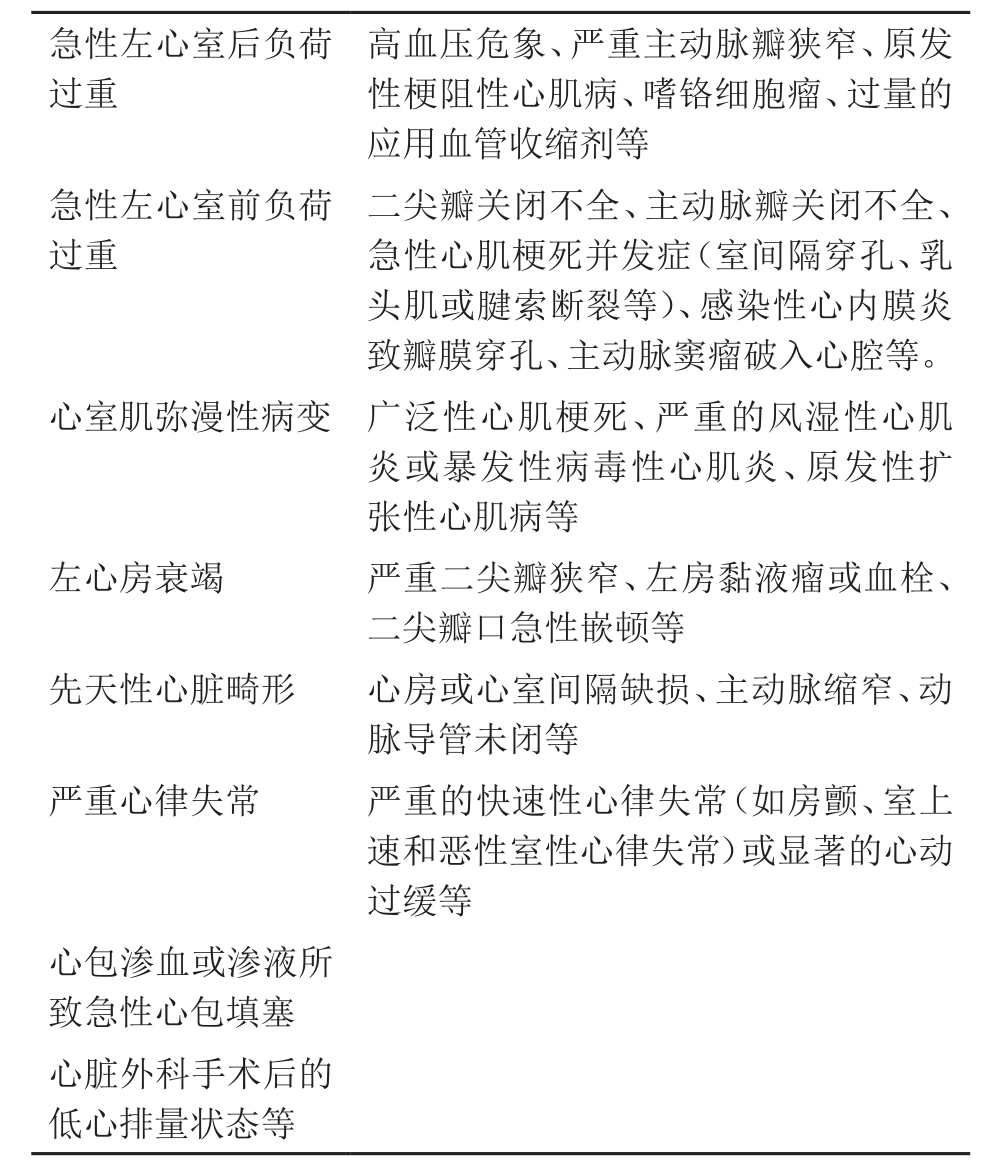
\includegraphics[width=3.28125in,height=3.875in]{./images/Image00093.jpg}
\end{table}

\subsection{病理生理}

正常心脏有丰富的储备力,使之能充分适应机体代谢状态的各种需要。当心肌收缩力减低和(或)负荷过重、心肌顺应性降低时,心脏储备力明显下降,此时机体首先通过代偿机制,包括Frank-Starling机制(增加心脏前负荷,回心血量增多,心室舒张末容积增加,从而增加心排血量及提高心脏做功量)、心肌肥厚、神经体液系统的代偿(包括交感神经兴奋性增强和肾素-血管紧张素系统激活)等,从而增加心肌收缩力和心率来维持心排血量。此外心房利钠肽(ANP)和脑利钠肽(BNP)、精氨酸加压素和内皮素等细胞因子也参与了心衰的发生与发展。近年对BNP的研究尤为活跃,BNP的作用主要表现为外周和中枢效应。外周效应包括:①促进尿钠排泄;②血管扩张;③抑制肾素-血管紧张素系统;④抗内皮细胞、平滑肌细胞、心肌细胞的有丝分裂从而抑制其增殖;中枢作用包括:①摄水抑制;②摄盐抑制;③降压效应;④抑制抗利尿激素(ADH)和促肾上腺皮质激素(ACTH)。此外随着充血性心衰的加重,血浆BNP的浓度也会升高,可以较正常升高200~300倍。

\begin{table}[htbp]
\centering
\caption{急性心力衰竭综合征根据临床表现的分类}
\label{tab26-2}
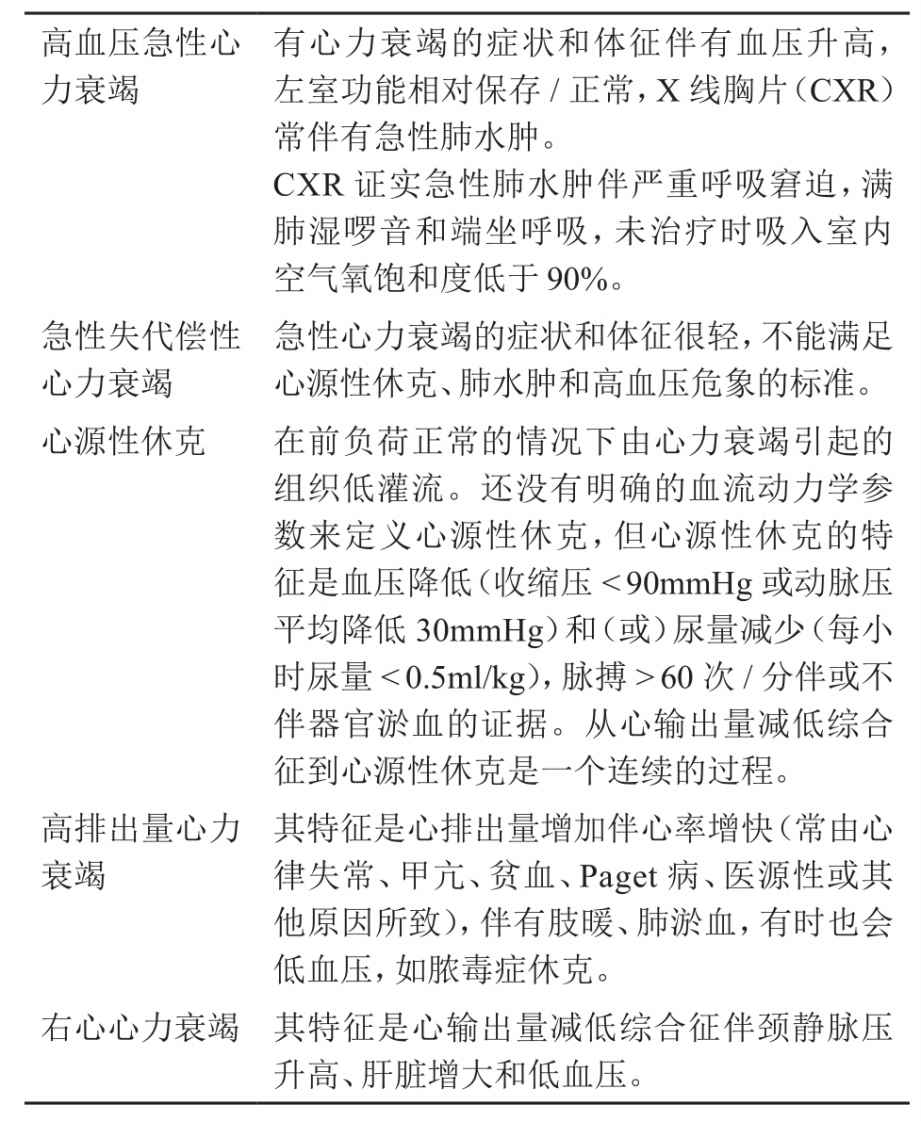
\includegraphics[width=3.25in,height=3.95833in]{./images/Image00094.jpg}
\end{table}

\begin{table}[htbp]
\centering
\caption{急性心力衰竭的初始临床表现分类}
\label{tab26-3}
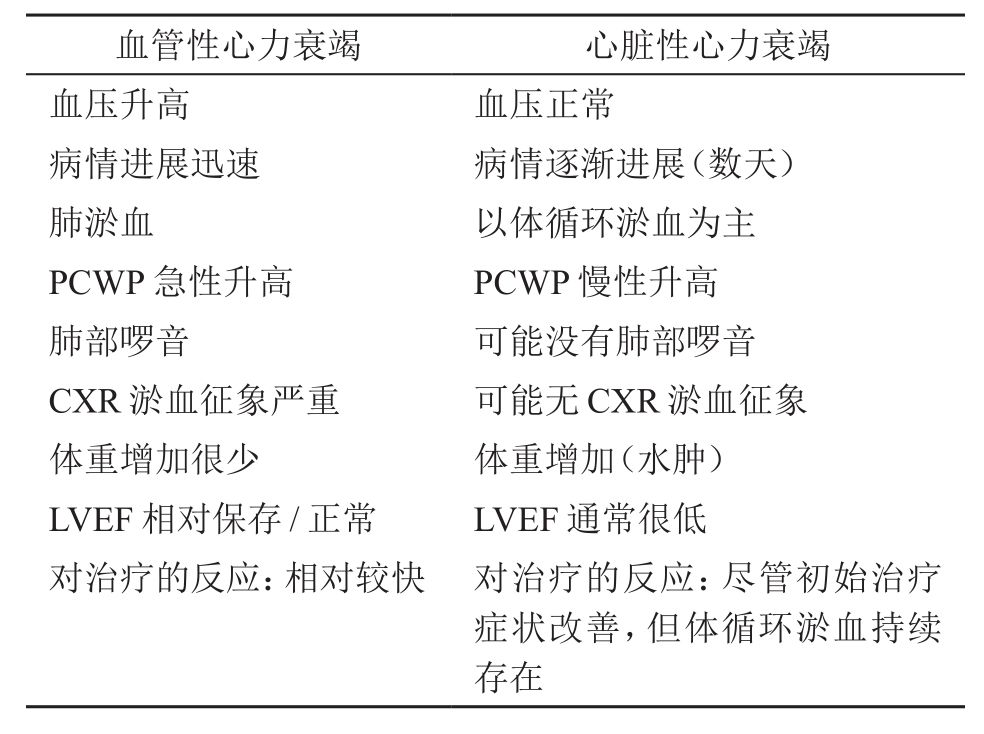
\includegraphics[width=3.27083in,height=2.4375in]{./images/Image00095.jpg}
\end{table}

虽然在心衰发生时心脏有以上这些代偿机制,但是这些代偿机制很有限,甚至可能会有害,当出现心脏失代偿时即发生心力衰竭。正常人肺毛细血管静水压一般不超过12mmHg,血浆胶体渗透压为25~30mmHg。由于两者压差的存在,有利于肺毛细血管对水分的重吸收,肺毛细血管的水分不能进入肺泡和肺间质。当急性左心衰竭发生时,左室舒张末压(LVEDP)和左房平均压升高,当肺静脉压大于18mmHg时,产生肺淤血。当肺毛细血管压超过血浆胶体渗透压时,血液中的水分即可从肺毛细血管渗透到肺间质;开始时通过淋巴流的增加引流肺间质内的液体。但是随着肺毛细血管压的继续升高,肺间质的淋巴循环不能引流过多的液体时,液体积聚于肺间质,在终末支气管和肺毛细血管的周围形成间质性肺水肿(interstitial
pulmonary
edema);当间质内液体继续聚集,肺毛细血管压继续增加大于25mmHg以上时,肺泡壁基底膜和毛细血管内皮间的连接被破坏,血浆和血液中的有形成分进入肺泡,因而发生肺水肿。原有慢性心功能不全的患者,如二尖瓣狭窄,其肺毛细血管壁和肺泡基底膜增厚,肺毛细血管静水压需大于35~40mmHg才发生肺水肿。此类患者肺毛细血管静水压突然升高可因一时性体力劳动、情绪激动或异位性心动过速(如房颤)引起肺循环血流量突然增多而诱发肺水肿。在肺泡内液体与气体形成泡沫后,表面张力增大,妨碍通气和肺毛细血管从肺泡内摄取氧,故可引起缺氧;同时肺水肿可减低肺的顺应性,引起换气不足和肺内动静脉分流,导致动脉血氧饱和度减低,组织乳酸产生过多而发生代谢性酸中毒,使心衰进一步恶化,甚至引起休克、严重心律失常而致死。

急性失代偿性心力衰竭(ADHF)是指由于心脏、外周血管床及其神经激素系统之间的相互作用失去平衡,导致体循环不能满足身体组织需要的一种血流动力学状态。目前推荐以B型钠尿肽的浓度来诊断急性失代偿性心力衰竭,BNP水平明显升高则诊断为失代偿。ADHF可以发生在心力衰竭的任何阶段,但常见于结构性心脏病和有心力衰竭病史或症状的患者。这一概念指出心力衰竭急性加重的病理生理机制,更符合到急诊的心力衰竭患者,能更好指导医生的诊断和治疗。

急性左心衰竭时,心血管系统的血流动力学改变包括:①左室顺应性降低、dp/dt降低,LVEDP升高(单纯二尖瓣狭窄例外);②左房压(LAP)和容量增加;③肺毛细血管压或肺静脉压增高;④肺淤血,严重时急性肺水肿;⑤外周血管阻力(SVR)增加;⑥肺血管阻力(PVR)增加;⑦心率加速;⑧心脏每搏量(SV)、心排血量(CO)、心脏指数(CI)皆降低;⑨动脉压先升高后下降;⑩心肌耗氧量增加。

\subsection{诊断}

\subsubsection{病史}

病史可提供与急性左心衰竭病因或诱因有关的信息。患者常先有较轻的慢性心力衰竭的症状如劳力性呼吸困难或轻度阵发性夜间呼吸困难,或体循环淤血的征象。原无症状者“突然”发生急性心力衰竭常提示冠心病急性心肌梗死或腱索断裂;肺血管阻力正常的二尖瓣狭窄患者可以突然发病,常是由新发生的快速房颤所促发。

\subsubsection{临床表现特点}

急性肺水肿为急性左心衰竭的主要表现。从病理生理角度可将肺水肿分为细胞水肿、间质水肿、肺泡水肿、休克和终末期五期,其临床表现随病情的发展也逐渐加重。

\subparagraph{细胞内水肿期}

常有烦躁、失眠、不安、血压升高等。

\subparagraph{间质性肺水肿期}

为不同程度的呼吸困难及原有呼吸困难的加重。患者阵发性夜间呼吸困难,呼吸频率浅快,面色苍白,脉速,颈静脉充盈,中心静脉压升高,但肺部仅有哮鸣音而无湿啰音。

\subparagraph{肺泡内水肿期}

以呼吸困难、咳嗽、咳痰为基本症状。呼吸浅快,频率达30~40次/分或以上,临床表现为极度焦虑、口唇发绀、皮肤湿冷、大汗淋漓、端坐呼吸、咳大量白色或粉红色泡沫样痰,可从口腔或鼻腔中喷出。湿啰音始于肺底部,迅速布满全肺,具有“突然发生、广泛分布、大中小湿啰音与哮鸣音并存、变化速率快”的特点。心音快而弱,心尖部闻及舒张期奔马律,但常被肺内啰音掩盖而不易听到。

\subparagraph{心源性休克期}

患者意识模糊,可发生阿-斯综合征或心源性休克。

\subparagraph{终末期}

患者呈昏迷状态,因心肺功能不全、窒息而死亡。

\subsubsection{辅助检查}

\subparagraph{B型钠尿肽}

床旁快速尿钠肽检查对急性心力衰竭的诊断既简单又客观方便,而成为了急性失代偿心力衰竭的诊断标志物。BNP小于100pg/ml的患者,其心力衰竭可能性很小,呼吸困难应考虑一些非心源性的病因所致;BNP大于400pg/ml的患者,呼吸困难由心力衰竭引起的可能性会非常大。

\subparagraph{胸部 X线检查}

对急性左心衰竭的诊断颇有价值。间质性肺水肿的X线特征为肺尖血管影增重,整个肺血管影增重、模糊,肺间隙或小叶间隙存在Kerley
B或A线。肺泡性肺水肿时,两肺门可有大片云雾状蝶翼状阴影,或肺野有粗大结节型或粟粒结节型改变,也可以伴有少量胸腔积液。

\subparagraph{心电图检查}

有原基础心脏病表现,以及有助于了解有无心律失常、急性心肌缺血等表现。

\subparagraph{超声心动图}

左心室舒张末径增大,心室壁运动幅度极度减弱,左室射血分数明显减低及基础心脏病表现等。

\subparagraph{血流动力学监测}

肺毛细血管楔压(PCWP)增高,心脏指数(CI)下降。当PCWP >
18mmHg,CI正常,提示肺淤血;PCWP为25~35mmHg,CI为2.2~2.5L/(min•m\textsuperscript{2}
),提示肺水肿;PCWP > 18mmHg,CI < 2.0L/(min•m\textsuperscript{2}
),提示心源性休克,预后不良。

\subsubsection{急诊呼吸困难的识别}

在急诊30\%~70\%的呼吸困难都是由心力衰竭所致,怎样快速有效地识别这些呼吸困难的病因就成了大家所关注的问题。多项研究都调查了病史和体格检查对心力衰竭诊断的准确性和可靠性。在病史中,“既往有过心力衰竭”最为有用,在体格检查中,听诊闻及第三心音可能对心力衰竭诊断似然比最高,但却无阴性预测作用(LR−,0.88),现将病史和体格检查对急诊呼吸困难的诊断准确性列于表\ref{tab26-4},以助于急诊快速的识别和评估呼吸困难的患者。

\subsection{治疗}

急性左心衰竭肺水肿的抢救原则是迅速改善氧合作用(纠正缺氧),降低左房压和(或)左室充盈压,增加左室心搏量,减少循环血量,减少肺泡内液体渗出,保证气体交换,以及纠正诱因或治疗病因,缓解患者的焦虑情绪等,这些治疗措施必须同时施行。

\subsubsection{体位}

允许患者采取最舒适的体位,通常为端坐位,两腿下垂,保持此种体位10~20分钟后,可使肺血容量降低约25\%,但是单纯坐位而下肢不下垂则收益不大。

\subsubsection{氧疗}

急性左心衰竭肺水肿均存在严重缺氧,缺氧又促使肺水肿恶化,故积极纠正缺氧、阻断恶性循环是治疗的首要环节。

\subparagraph{氧疗的目标}

\begin{table}[htbp]
\centering
\caption{病史和体格检查对急诊呼吸困难的诊断准确性}
\label{tab26-4}
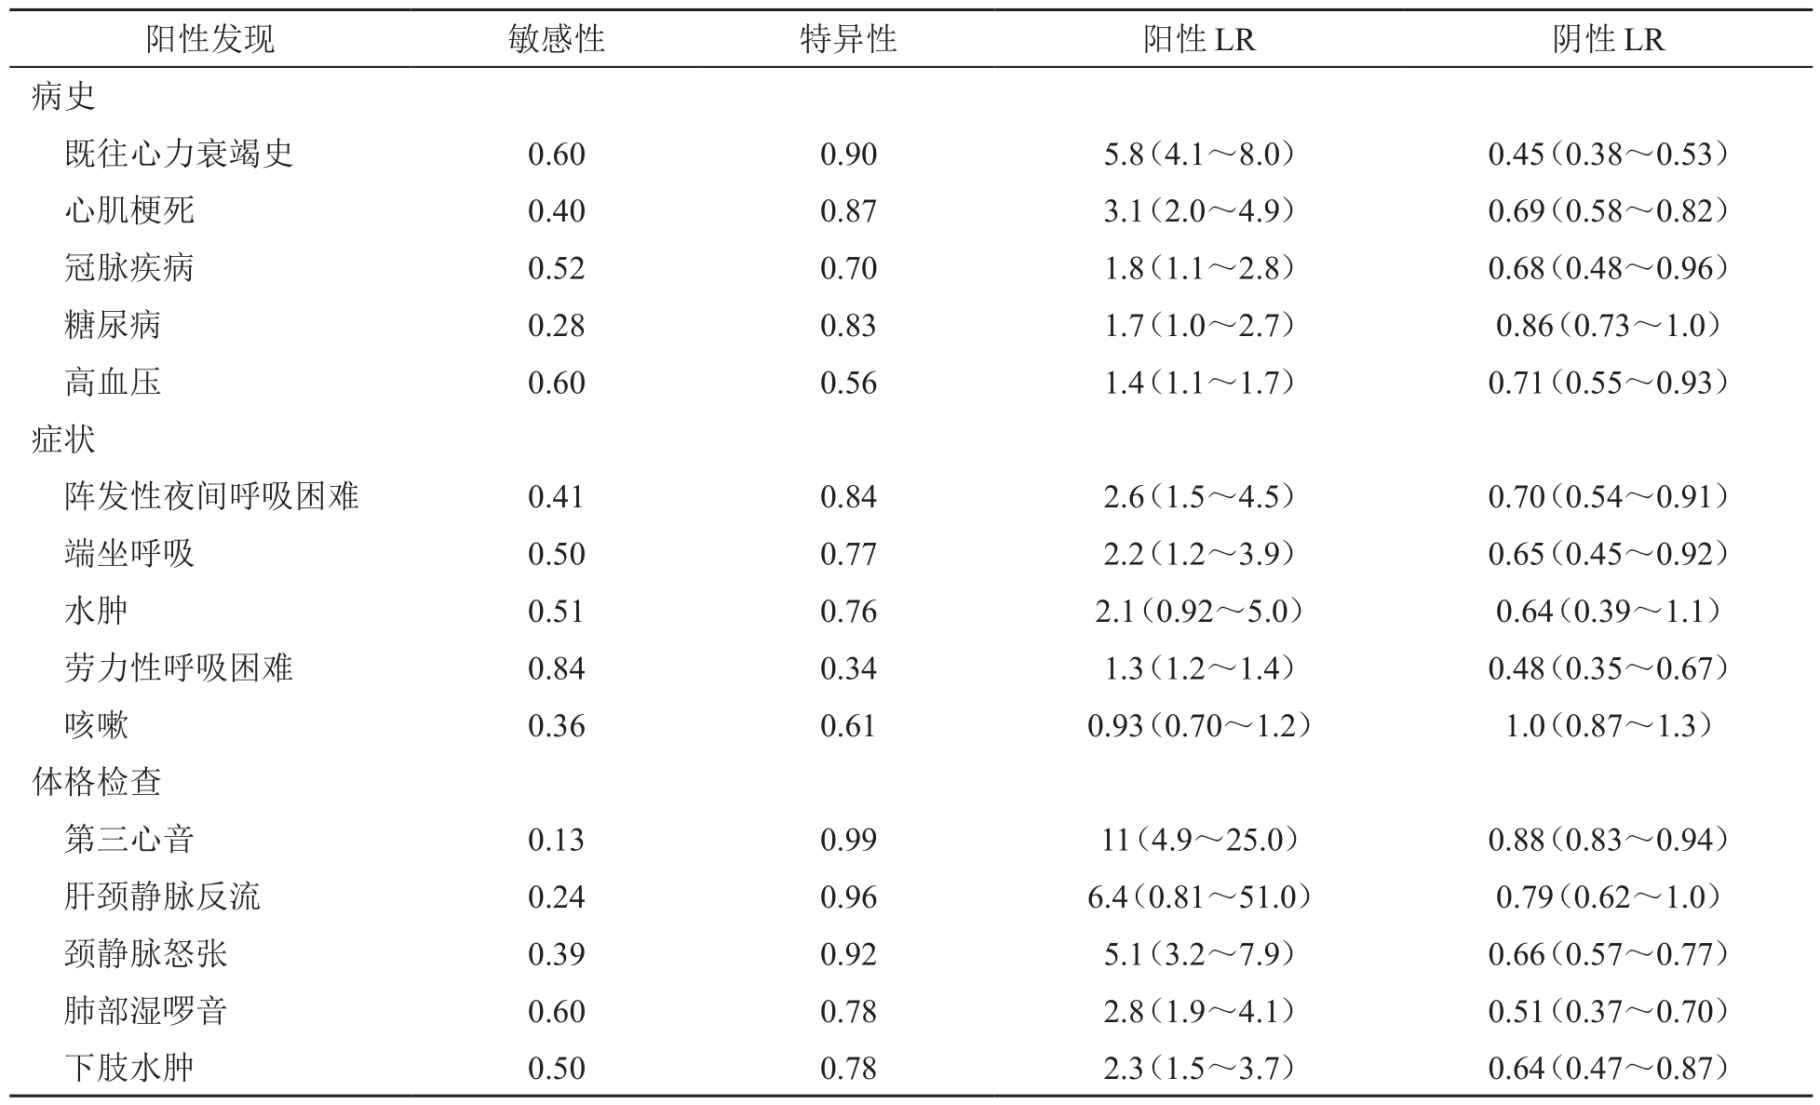
\includegraphics[width=6.51042in,height=3.94792in]{./images/Image00096.jpg}
\end{table}

单纯缺氧者使PaO\textsubscript{2}
提高至正常范围95~100mmHg;伴有CO\textsubscript{2}
潴留者,使PaO\textsubscript{2} 上升到60mmHg,以不超过70~80mmHg为宜。

\subparagraph{给氧方法}

①鼻导管吸氧:是常用的给氧方法,适用于轻中度缺氧者,氧流量为4~6L/min,常加用除泡剂。②面罩吸氧:可以提高吸入氧气的浓度,神志清醒者多不能耐受,适用于昏睡的患者。经上述方法给氧后PaO\textsubscript{2}
仍< 60mmHg时,应考虑使用机械通气治疗。

\subparagraph{消除泡沫}

严重肺水肿患者的肺泡、支气管内含有大量液体,当液体表面张力达到一定程度时,受气流冲击可形成大量泡沫,泡沫妨碍通气和气体交换,乃加重缺氧。因此,可于吸氧的湿化器内加入50\%的酒精以降低泡沫张力,使之破裂变为液体而易咳出,减轻呼吸道阻力,改善通气和换气;酒精尚有缓解支气管痉挛,扩张末梢血管和镇静作用。

\subsubsection{药物治疗}

\subparagraph{吗啡}

除给氧外,治疗急性左心衰肺水肿的最有效药物是咖啡。其主要作用机制是抑制中枢交感神经,反射性地降低周围血管阻力,增加射血分数,扩张静脉而减少回心血量,起“药物静脉内放血”的作用;其他作用有减轻焦虑、烦躁,抑制反射性呼吸中枢兴奋、避免呼吸过频,直接松弛支气管平滑肌改善通气。急性左心衰竭患者往往存在外周血管收缩情况,吗啡从皮下或肌肉注射后,吸收情况无法预测。现多主张静脉给予:3~5mg/次缓慢静脉注射,必要时每15分钟重复1次,供2~3次;病情不甚危急时,也可以10mg皮下或肌肉注射,每3~4小时可重复给药。但勿皮下或肌肉注射后,短期内又静脉给药,因静注后可能与延迟吸收的第一剂药同时发挥作用而致呼吸抑制,应随时备用吗啡拮抗剂(纳洛酮)。吗啡的主要副作用是低血压与呼吸抑制。伴有神志不清、慢性阻塞性肺病、呼吸衰竭、肝功能衰竭、颅内出血、低血压休克者禁用,年老体弱者慎用。心动过缓者可用吗啡加阿托品0.5mg合用皮下注射,以增快心率、扩张支气管及减少恶心、呕吐等症状。无吗啡时,可用哌替啶(度冷丁)50~100mg肌肉注射。

\subparagraph{快速利尿}

选用高效利尿剂(袢利尿剂)。呋塞米(速尿)不仅可以利尿,而且在发挥利尿作用之前即可通过扩张周围静脉增加静脉床容量,迅速降低肺毛细血管压和左室充盈压并改善症状。静注后5分钟开始利尿,30~60分钟达到高峰,作用持续约2小时。一般首剂量为20~40mg。对正在使用呋塞米或有大量水钠潴留或高血压或肾功能不全的患者,首剂量可增加2~3倍。应注意防止过度利尿可能发生的低血容量、休克与电解质紊乱如低钾血症。也可以用布美他尼(丁尿胺)1~2mg或依他尼酸25~100mg静注。伴有低血容量或低血压休克或PCWP
<
15~18mmHg者禁用。高渗性利尿剂如甘露醇可增加血容量,急性左心衰时不宜使用。

\subparagraph{氨茶碱}

本品具有:①扩张支气管改善通气,特别适用于伴有支气管痉挛的患者;②轻度扩张静脉,降低心脏前负荷,增强心肌收缩力;③增加肾血流与利尿作用。用法:首剂4~6mg/kg(成人一般用0.25g)加入25\%葡萄糖液40ml内,10~20分钟内缓慢静注;必要时4~6小时可以重复1次,但每日总量不宜超过1~1.5g。因会增加心肌耗氧量,急性心肌梗死和心肌缺血者不宜使用。老年人与肝肾功能不全者用量酌减。氨茶碱常见的副作用有头痛、面部潮红、心悸、心前区疼痛,严重者可因血管扩张致低血压与休克,甚至室性心律失常而猝死。

\subparagraph{血管扩张剂}

常用的有:

\hypertarget{text00070.htmlux5cux23CHP3-2-4-3-4-1}{}
(1) 硝酸甘油:

是治疗急性左心衰常用的血管扩张剂。其作用主要是扩张静脉容量血管、降低心脏前负荷,较大剂量时可同时降低后负荷;尚可增强肾脏对利尿剂的反应。特别适用于严重呼吸困难,PCWP显著升高而心排出量与血压正常或接近正常者(SBP≥100mmHg)。用法有:①舌下含化:首次用0.3mg舌下含化,5分钟后测量血压1次,再给0.6mg,5分钟后再测血压,以后每10分钟给0.6mg,直到症状改善或收缩压降至90~100mmHg。②静脉给药:一般采用微量泵输注,从10µg/min开始,以后每5分钟递增5~10µg/min,直至急性心力衰竭的症状缓解或收缩压降至90~100mmHg,或达到最大剂量100µg/min为止。病情稳定后逐步减量至停用,突然终止用药可能会出现症状反跳。

\hypertarget{text00070.htmlux5cux23CHP3-2-4-3-4-2}{}
(2) 硝普钠:

能均衡的扩张动脉和静脉,同时降低心脏前、后负荷,最适用于高血压、急性二尖瓣反流或急性主动脉瓣反流所致的急性左心衰竭。给药方法为静脉给药,常使用微量泵输注,输注速度从10µg/min开始,以后每5分钟递增5~10µg/min,直至症状缓解、血压由原水平下降30mmHg或血压降至90~100mmHg时为止,硝普钠常用的维持剂量3µg/(kg•min),极量为10µg/(kg•min)。有效剂量维持至病情稳定,以后逐渐减量、停药。突然停药可引起反跳。长期用药可引起氰化物和硫氰酸盐中毒,因而近年来已渐被硝酸甘油取代。

\hypertarget{text00070.htmlux5cux23CHP3-2-4-3-4-3}{}
(3) 酚妥拉明:

为α受体阻断剂,主要降低后负荷。静滴5分钟内显效,一般从0.1mg/min开始,每5分钟逐渐增加剂量,最大速度不超过2mg/min。其主要的副作用是低血压和心动过速,故近年已较少使用。

\hypertarget{text00070.htmlux5cux23CHP3-2-4-3-4-4}{}
(4) 硝酸异山梨酯:

主要扩张静脉容量血管,降低心脏前负荷,同时增加心肌血供。舌下含化每次10~20mg,4~6小时1次,直至症状缓解。

\hypertarget{text00070.htmlux5cux23CHP3-2-4-3-4-5}{}
(5) 乌拉地尔:

为α\textsubscript{1}
受体阻滞剂,通常静脉注射25mg,如血压无明显降低可重复注射,然后予50~100mg
于100ml液体中静脉滴注维持,速度为0.4~2mg/min,根据血压调整速度。

\subparagraph{正性肌力药物}

常用的有:

\hypertarget{text00070.htmlux5cux23CHP3-2-4-3-5-1}{}
(1) 洋地黄类制剂:

近年来由于快速强力利尿剂与血管扩张剂的广泛应用,洋地黄在抢救急性心力衰竭中的地位已有所下降。主要适应证是由快速型室上性心律失常所致的心衰,如快速房颤致急性肺水肿的二尖瓣狭窄的患者。近两周内未用过洋地黄的患者,可选用毛花苷丙(西地兰)0.4~0.8mg加入25\%~50\%葡萄糖液20~40ml中缓慢静注;必要时2~4小时后再给0.2~0.4mg,直至心室率控制在80次/分左右或总量达到1.2~1.6mg。若近期用过洋地黄,但并非洋地黄中毒所致心力衰竭,仍可应用洋地黄,但应酌情减量。在用洋地黄之前,应作心电图确定心律,了解是否有急性心肌梗死、心肌炎或低血钾等。此外风湿性心脏病单纯性二尖瓣狭窄合并急性肺水肿时,如为窦性心律不宜使用洋地黄制剂,因洋地黄能增加心肌收缩力,使右室排血量增加,加重肺水肿;但若二尖瓣狭窄合并二尖瓣关闭不全的肺水肿患者,可用洋地黄制剂。

\hypertarget{text00070.htmlux5cux23CHP3-2-4-3-5-2}{}
(2) 儿茶酚胺类:

常用者为多巴胺和多巴酚丁胺,两者常以2.5~10µg/(kg•min)静脉给予,与血管扩张剂联合使用效果更佳。有关其用法与注意事项详见第157章“拟肾上腺素药”。

\hypertarget{text00070.htmlux5cux23CHP3-2-4-3-5-3}{}
(3) 磷酸二酯酶抑制剂:

这些药物选择性抑制心肌和平滑肌的磷酸二酯酶同工酶Ⅲ,减少cAMP的降解而提高细胞内cAMP的含量,发挥强心与直接扩血管作用。常用的药物有二氢吡啶类的氨力农、米利农,咪唑类的依诺昔酮等,但这类药物不可长期应用,仅适合于治疗急性心力衰竭。米利农甚至可加速心衰恶化,增加死亡率。

\subparagraph{地塞米松}

具有解除支气管痉挛,降低肺毛细血管通透性、改善肾血流、促进利尿等作用。可酌情短期使用。常用10~20mg加入液体中静滴。

\subsubsection{人工合成BNP的治疗作用}

奈西立肽是FDA批准的一种重组BNP,用于治疗急性失代偿性充血性心力衰竭,具有降低肺毛细血管楔压,减轻血管阻力,降低心房压和肺动脉压,增加心脏指数和每搏输出量,从而产生有益的血流动力学效应。使用剂量为0.015µg/(kg•min)。

\subsubsection{减少静脉回流}

除接受静脉输液的肢体外,用软质橡皮管止血带或充气式袖带结扎其余三支的近端,加压的压力比舒张压约高10mmHg左右为宜。每15~20分钟轮流放松一肢。可使近700ml的血液扣留在肢端。目前此法已少用,但在病情危急而其他治疗措施不能马上实施时可一试。有严重周围动脉闭塞性疾病的患者禁用。

\subsubsection{静脉穿刺放血法}

已经很少使用,经积极治疗20~30分钟后症状仍无缓解且加重者,可考虑放血300~500ml,尤其是大量输液和输血所致的肺水肿。低血压和贫血时禁用。

\subsubsection{透析治疗}

主要适用于慢性肾功能不全容量负荷过多的患者。

\subsubsection{机械通气治疗}

机械通气可以迅速改善低氧血症,同时机械通气的压力可以改善气体交换,增加通气量,又可以降低左心室的后负荷改善冠脉循环和心肌缺血。包括有创机械通气和经面(鼻)罩机械通气治疗。

\subparagraph{经面}

(鼻)罩机械通气
适用于患者神志清楚,自主呼吸能力强,通气时间短,容易配合面(鼻)罩机械通气。主要适用于轻、中度患者,同时心电活动稳定。首选鼻罩,其次为选用面罩。多数患者选用BiPAP呼吸机,尽量选择流量触发,首选PSV
+ PEEP模式,气道峰压尽量不超过30cmH\textsubscript{2} O。

\subparagraph{有创机械通气治疗的指征}

包括:①心电活动不稳定,如急性心肌梗死和严重心律失常。②严重低氧血症,面罩吸氧时PaO\textsubscript{2}
仍小于60mmHg。③出现高碳酸血症。④有严重的基础肺疾病,或同时或先后发生心肺功能不全。⑤严重并发症或应用镇静-肌松剂抑制呼吸道分泌物的排出。治疗中应选用经口气管插管或气管切开插管。初始宜用间歇正压呼吸给氧,它能使更多的肺泡开放,加大肺泡平均容量,以利气体交换,一般将吸气相正压控制在30cmH\textsubscript{2}
O以下。若仍无效,可改用呼气末正压呼吸(PEEP)给氧,PEEP改善换气功能的作用和左心功能的作用随其大小的增加而增强。适当增加的PEEP可减少回心血量,减轻心脏前负荷,可增加心输出量。PEEP设置的原则一般从零开始,短期内增加到5cmH\textsubscript{2}
O左右,在使用PEEP期间要严格监测血压,若血压和心率稳定,间隔20~30分钟增加一次,每次增加2cmH\textsubscript{2}
O,一般达到10cmH\textsubscript{2} O,多数无需超过15cmH\textsubscript{2}
O。

\subsubsection{急性心力衰竭的急诊治疗流程}

急诊对急性心力衰竭处置的最主要问题是早期识别和评估,及早稳定患者和快速处理,我们列出了急诊心力衰竭的治疗流程,以供大家参考(图\ref{fig26-1})。

\subsubsection{病因和诱因治疗}

诱因治疗包括控制感染、纠正贫血与心律失常等,病因治疗如极度严重的二尖瓣狭窄或主动脉瓣狭窄,或AMI并发严重二尖瓣反流的患者可能需要外科治疗才能缓解肺水肿,可行急诊手术治疗。

\begin{figure}[!htbp]
 \centering
 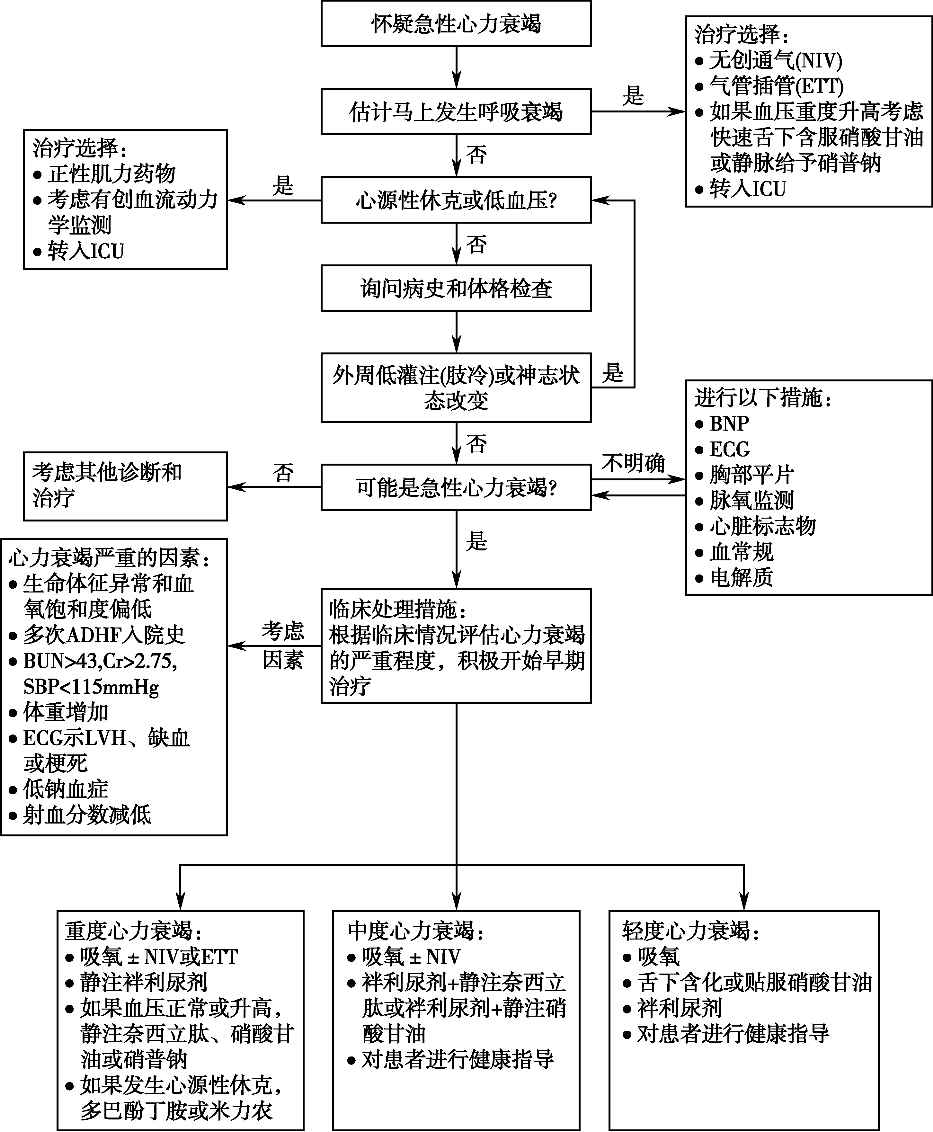
\includegraphics[width=4.83333in,height=5.86458in]{./images/Image00097.jpg}
 \captionsetup{justification=centering}
 \caption{急性心力衰竭的急诊治疗流程}
 \label{fig26-1}
  \end{figure} 

\protect\hypertarget{text00071.html}{}{}

\hypertarget{text00071.htmlux5cux23CHP3-2-5}{}
附:急性心力衰竭诊断和治疗指南

(中华医学会心血管病学分会.中华心血管病杂志,2010,38(3):195-208)

\subsection{前言}

急性心力衰竭(心衰)临床上以急性左心衰竭最为常见,急性右心衰竭则较少见。急性左心衰竭指急性发作或加重的左心功能异常所致的心肌收缩力明显降低、心脏负荷加重,造成急性心排血量骤降、肺循环压力突然升高、周围循环阻力增加,引起肺循环充血而出现急性肺淤血、肺水肿并可伴组织器官灌注不足和心源性休克的临床综合征。急性右心衰竭是指某些原因使右心室心肌收缩力急剧下降或右心室的前后负荷突然加重,从而引起右心排血量急剧减低的临床综合征。急性心衰可以突然起病或在原有慢性心衰基础上急性加重;大多数表现为收缩性心衰,也可以表现为舒张性心衰;发病前患者多数合并有器质性心血管疾病。对于在慢性心衰基础上发生的急性心衰,经治疗后病情稳定,不应再称为急性心衰。

急性心衰常危及生命,必须紧急施救和治疗。近10余年,尽管对于慢性心衰的基础和临床研究已取得长足进步,但急性心衰的临床工作仍存在以下问题:①临床研究,尤其大样本前瞻性随机对照试验很少,临床证据匮乏,使得目前各国指南中关于治疗的推荐大多基于经验或专家意见,缺少充分的证据支持;②我国自己的研究严重滞后,缺少临床资料,甚至基本的流行病学材料也不够齐全;急性心衰的处理各地缺少规范,急性心衰的病死率虽有下降但仍是心源性死亡的重要原因,成为我国心血管病急症治疗的一个薄弱环节。鉴于上述理由,中华医学会心血管病学分会决定编撰我国的“急性心力衰竭诊断和治疗指南”,以提高对这一心脏病急重症临床处理的水平。

中华医学会心血管病学分会心衰专业组组建了这一工作的撰写组和专家组,并确定了对指南编写的基本原则:①要充分汲取这一领域的新进展、新技术、新方法,借鉴国外主要心血管病学术组织近几年制定和颁布的各种指南;②要根据我国的国情和临床处理的传统习惯以及已证实行之有效的方法与经验,包括我国近几年编写的心衰及相关疾病的指南与专家共识,使其符合我国国情;③为基层单位和各级医院临床医师提供能够接受和乐意使用的指导性文件。

本指南按国际通用的方式,标示了药物和各种治疗方法应用的推荐类别和证据水平分级。推荐类别:Ⅰ类为已证实和(或)一致认为有益和有效;Ⅱ类为疗效的证据尚不一致或有争议,其中相关证据倾向于有效的为Ⅱa类,尚不充分的为Ⅱb类;Ⅲ类为已证实或一致认为无用和无效,甚至可能有害。证据水平分级:证据来自多项随机对照临床试验或多项荟萃分析为A级;证据来自单项随机对照临床试验或非随机研究为B级;证据来自小型研究或专家共识为C级。

\subsection{急性心衰的流行病学}

美国过去10年中,因急性心衰而急诊就医者达1千万例次。急性心衰患者中约15\%~20\%为首诊心衰,大部分则为原有的心衰加重。所有引起慢性心衰的疾病都可导致急性心衰。晚近,随慢性心衰患者数量逐渐增加,慢性心功能失代偿和急性心衰发作,业已成为心衰患者住院的主因,每年心衰的总发病率为0.23\%~0.27\%。急性心衰预后很差,住院病死率为3\%,60天病死率为9.6\%,3年和5年病死率分别高达30\%和60\%。急性心肌梗死所致的急性心衰则病死率更高。急性肺水肿患者的院内病死率为12\%,1年病死率达30\%。

我国对42家医院1980年、1990年、2000年3个时段住院病历所作回顾性分析表明,因心衰住院约占住院心血管病患者的16.3\%~17.9\%,其中男性占56.7\%,平均年龄为63~67岁,60岁以上者超过60\%;平均住院时间分别为35.1天、31.6天和21.8天。心衰病种主要为冠心病、风湿性心瓣膜病和高血压病。在这20年时间中,冠心病和高血压病分别从36.8\%和8.0\%增至45.6\%和12.9\%,而风湿性心脏病则从34.4\%降至18.6\%;入院时的心功能都以Ⅲ级居多(42.5\%~43.7\%)。此种住院患者基本为慢性心衰的急性加重。

\subsection{急性心衰的病因和病理生理学机制}

\subsubsection{急性左心衰竭的常见病因}

1.慢性心衰急性加重。

2.急性心肌坏死和(或)损伤
①急性冠状动脉综合征如急性心肌梗死或不稳定性心绞痛、急性心肌梗死伴机械性并发症、右心室梗死;②急性重症心肌炎;③围生期心肌病;④药物所致的心肌损伤与坏死,如抗肿瘤药物和毒物等。

3.急性血流动力学障碍
①急性瓣膜大量反流和(或)原有瓣膜反流加重,如感染性心内膜炎所致的二尖瓣和(或)主动脉瓣穿孔、二尖瓣腱索和(或)乳头肌断裂、瓣膜撕裂(如外伤性主动脉瓣撕裂)以及人工瓣膜的急性损害等;②高血压危象;③重度主动脉瓣或二尖瓣狭窄;④主动脉夹层;⑤心包压塞;⑥急性舒张性左心衰竭,多见于老年控制不良的高血压患者。

\subsubsection{急性左心衰竭的病理生理机制}

\subparagraph{急性心肌损伤和坏死}

缺血性心脏病合并急性心衰主要有下列3种情况:①急性心肌梗死:主要见于大面积的心肌梗死;有时急性心肌梗死也可首先表现为急性左心衰竭症状,尤其老年患者和糖尿病患者;②急性心肌缺血:缺血面积大、缺血严重也可诱发急性心衰,此种状况可见于梗死范围不大的老年患者,虽然梗死面积较小,但缺血面积大;③原有慢性心功能不全,如陈旧性心肌梗死或无梗死史的慢性缺血性心脏病患者,在缺血发作或其他诱因下可出现急性心衰。此外,一些以急性左心衰竭为主要表现的患者可能没有明显的胸痛症状,但当存在相应危险因素的情况下可能是缺血性心脏病所致。

心肌缺血及其所产生的心肌损伤使部分心肌处在心肌顿抑和心肌冬眠状态,并导致心功能不全。当冠状动脉血流及氧合恢复,冬眠心肌功能迅速改善,而顿抑心肌心功能不全仍继续维持一段时间,但对正性肌力药物有反应。严重和长时间的心肌缺血必将造成心肌不可逆的损害。

急性心肌梗死或急性重症心肌炎等可造成心肌坏死,使心脏的收缩单位减少。高血压急症或严重心律失常等均可使心脏负荷增加。这些改变可产生血流动力学紊乱,还可激活肾素-血管紧张素-醛固酮系统(RAAS)和交感神经系统,促进心衰患者病情加剧和恶化。上述病理生理过程可因基础病变重笃而不断进展,或在多种诱因的激发下迅速发生而产生急性心衰。

\subparagraph{血流动力学障碍}

急性心衰主要的血流动力学紊乱有:①心排血量(CO)下降,血压绝对或相对下降以及外周组织器官灌注不足,导致出现脏器功能障碍和末梢循环障碍,发生心源性休克。②左心室舒张末压和肺毛细血管楔压(PCWP)升高,可发生低氧血症、代谢性酸中毒和急性肺水肿。③右心室充盈压升高,使体循环静脉压升高、体循环和主要脏器淤血、水钠滞留和水肿等。

\subparagraph{神经内分泌激活}

交感神经系统和RAAS的过度兴奋是机体在急性心衰时的一种保护性代偿机制,当长期的过度兴奋就会产生不良影响,使多种内源性神经内分泌与细胞因子激活,加重心肌损伤、心功能下降和血流动力学紊乱,这又反过来刺激交感神经系统和RAAS的兴奋,形成恶性循环。

\subparagraph{心肾综合征}

心衰和肾功能衰竭常并存,并互为因果。临床上将此种状态称之为心肾综合征。心肾综合征可分为5种类型:1型的特征是迅速恶化的心功能导致急性肾功能损伤;2型的特征为慢性心衰引起进展性慢性肾病;3型是原发、急速的肾功能恶化导致急性心功能不全;4型系由慢性肾病导致心功能下降和(或)心血管不良事件危险增加;5型特征是由于急性或慢性全身性疾病导致心肾功能同时出现衰竭。显然,3型和4型心肾综合征均可引起心衰,其中3型可造成急性心衰。5型心肾综合征也可诱发心衰甚至急性心衰。

\subparagraph{慢性心衰的急性失代偿}

稳定的慢性心衰可以在短时间内急剧恶化,心功能失代偿,表现为急性心衰。其促发因素中较多见为药物治疗缺乏依从性、严重心肌缺血、重症感染、严重的影响血流动力学的各种心律失常、肺栓塞以及肾功能损伤等。

\subsubsection{急性右心衰竭的病因和病理生理机制}

急性右心衰竭多见于右心室梗死、急性大块肺栓塞和右侧心瓣膜病。

右心室梗死很少单独出现,常合并于左心室下壁梗死。患者往往有不同程度的右心室功能障碍,其中约10\%~15\%可出现明显的血流动力学障碍。此类患者血管闭塞部位多在右冠状动脉开口或近段右心室侧支发出之前。右心室梗死所致的右心室舒缩活动障碍使右心室充盈压和右心房压升高;右心室排血量减少导致左心室舒张末容量下降、PCWP降低。

急性大块肺栓塞使肺血流受阻,出现持续性严重肺动脉高压,使右心室后负荷增加和扩张,导致右心衰竭;右心排血量降低导致体循环和心功能改变,出现血压下降、心动过速、冠状动脉灌注不足;对呼吸系统的影响主要是气体交换障碍;各种血管活性药物的释出,使广泛的肺小动脉收缩,增加了缺氧程度,又反射性促进肺动脉压升高,形成恶性循环。

右侧心瓣膜病所致急性右心衰竭不常见,且多为慢性右心衰竭,只有急性加重时才表现为急性右心衰竭。

\subsection{急性心衰的临床分类与诊断}

\subsubsection{临床分类}

国际上尚无统一的急性心衰临床分类。根据急性心衰的病因、诱因、血流动力学与临床特征作出的分类便于理解,也有利于诊断和治疗。

1.急性左心衰竭
①慢性心衰急性失代偿;②急性冠状动脉综合征;③高血压急症;④急性心瓣膜功能障碍;⑤急性重症心肌炎和围生期心肌病;⑥严重心律失常。

2.急性右心衰竭。

3.非心源性急性心衰
①高心排血量综合征;②严重肾脏疾病(心肾综合征);③严重肺动脉高压;④大块肺栓塞等。

\subsubsection{急性左心衰竭的临床表现}

\subparagraph{基础心血管疾病的病史和表现}

大多数患者有各种心脏病的病史,存在引起急性心衰的各种病因。老年人中的主要病因为冠心病、高血压和老年性退行性心瓣膜病,而在年轻人中多由风湿性心瓣膜病、扩张型心肌病、急性重症心肌炎等所致。

\subparagraph{诱发因素}

常见的诱因有:①慢性心衰药物治疗缺乏依从性;②心脏容量超负荷;③严重感染,尤其肺炎和败血症;④严重颅脑损害或剧烈的精神心理紧张与波动;⑤大手术后;⑥肾功能减退;⑦急性心律失常如室性心动过速(室速)、心室颤动(室颤)、心房颤动(房颤)或心房扑动伴快速心室率、室上性心动过速以及严重的心动过缓等;⑧支气管哮喘发作;⑨肺栓塞:⑩高心排血量综合征如甲状腺功能亢进危象、严重贫血等;{}
应用负性肌力药物如维拉帕米、地尔硫{} 、β受体阻滞剂等;{}
应用非甾体类抗炎药;{} 心肌缺血(通畅无症状);{}
老年急性舒张功能减退;{} 吸毒;{} 酗酒;{}
嗜铬细胞瘤。这些诱因使心功能原来尚可代偿的患者骤发心衰,或者使已有心衰的患者病情加重。

\subparagraph{早期表现}

原来心功能正常的患者出现原因不明的疲乏或运动耐力明显减低以及心率增加15~20次/分,可能是左心功能降低的最早期征兆。继续发展可出现劳力性呼吸困难、夜间阵发性呼吸困难、睡觉需用枕头抬高头部等;检查可发现左心室增大、闻及舒张早期或中期奔马律、P\textsubscript{2}
亢进、两肺尤其肺底部有细湿啰音,还可有干湿啰音和哮鸣音,提示已有左心功能障碍。

\subparagraph{急性肺水肿}

起病急骤,病情可迅速发展至危重状态。突发的严重呼吸困难、端坐呼吸、喘息不止、烦躁不安并有恐惧感,呼吸频率可达30~50次/分;频繁咳嗽并咯出大量粉红色泡沫样血痰;听诊心率快,心尖部常可闻及奔马律;两肺满布湿啰音和哮鸣音。

\subparagraph{心源性休克}

主要表现为:

(1)
持续低血压,收缩压降至90mmHg以下,或原有高血压的患者收缩压降幅≥60mmHg,且持续30分钟以上。

(2)
组织低灌注状态,可有:①皮肤湿冷、苍白和发绀,出现紫色条纹;②心动过速>
110次/分;③尿量显著减少(<
20ml/h),甚至无尿;④意识障碍,常有烦躁不安、激动焦虑、恐惧和濒死感;收缩压低于70mmHg,可出现抑制症状如神志恍惚、表情淡漠、反应迟钝,逐渐发展至意识模糊甚至昏迷。

(3)
血流动力学障碍:PCWP≥18mmHg,心脏排血指数(CI)≤36.7ml(/s•m\textsuperscript{2}
){[}≤2.2L(/min•m\textsuperscript{2} ){]};

(4) 低氧血症和代谢性酸中毒。

\subsubsection{急性左心衰竭的实验室辅助检查}

\subparagraph{心电图}

能提供许多重要信息,包括心率、心脏节律、传导,以及某些病因依据如心肌缺血性改变、ST段抬高或非ST段抬高心肌梗死以及陈旧性心肌梗死的病理性Q波等。还可检测出心肌肥厚、心房或心室扩大、束支传导阻滞、心律失常的类型及其严重程度如各种房性或室性心律失常(房颤、房扑伴快速性心室率、室速)、QT间期延长等。

\subparagraph{胸部 X线检查}

可显示肺淤血的程度和肺水肿,如出现肺门血管影模糊、蝶形肺门,甚至弥漫性肺内大片阴影等。还可根据心影增大及其形态改变,评估基础的或伴发的心脏和(或)肺部疾病以及气胸等。

\subparagraph{超声心动图}

可用以了解心脏的结构和功能、心瓣膜状况、是否存在心包病变、急性心肌梗死的机械并发症以及室壁运动失调;可测定左室射血分数(LVEF),检测急性心衰时的心脏收缩/舒张功能相关的数据。超声多普勒成像可间接测量肺动脉压、左右心室充盈压等。此法为无创性,应用方便,有助于快速诊断和评价急性心衰,还可用来监测患者病情的动态变化,对于急性心衰是不可或缺的监测方法。一般采用经胸超声心动图,如患者疑为感染性心内膜炎,尤为人工瓣膜心内膜炎,在心衰病情稳定后还可采用经食管超声心动图,能够更清晰显示赘生物和瓣膜周围的脓肿等。

\subparagraph{动脉血气分析}

急性左心衰竭常伴低氧血症,肺淤血明显者可影响肺泡氧气交换。应监测动脉氧分压(PaO\textsubscript{2}
)、二氧化碳分压(PaCO\textsubscript{2}
)和氧饱和度,以评价氧含量(氧合)和肺通气功能。还应检测酸碱平衡状况,本症患者常有酸中毒,与组织灌注不足、二氧化碳潴留有关,且可能与预后相关,及时处理纠正很重要。无创测定血氧饱和度可用作长时间、持续和动态监测,由于使用简便,一定程度上可以代替动脉血气分析而得到广泛应用,但不能提供PaCO\textsubscript{2}
和酸碱平衡的信息。

\subparagraph{常规实验室检查}

包括血常规和血生化检查,如电解质(钠、钾、氯等)、肝功能、血糖、白蛋白及高敏C反应蛋白(hs-CRP)。研究表明,hs-CRP对评价急性心衰患者的严重程度和预后有一定的价值。

\subparagraph{心衰标志物}

B型利钠肽(BNP)及其N末端B型利钠肽原(NT-proBNP)的浓度增高已成为公认诊断心衰的客观指标,也是心衰临床诊断上近几年的一个重要进展。其临床意义如下:①心衰的诊断和鉴别诊断:如BNP
< 100ng/L或NT-proBNP <
400ng/L,心衰可能性很小,其阴性预测值为90\%;如BNP > 400ng/L或NT-proBNP
>
1500ng/L,心衰可能性很大,其阳性预测值为90\%。急诊就医的明显气急患者,如BNP/NT-proBNP水平正常或偏低,几乎可以除外急性心衰的可能性。②心衰的危险分层:有心衰临床表现、BNP/NT-proBNP水平又显著增高者属高危人群。③评估心衰的预后:临床过程中这一标志物持续走高,提示预后不良。

\subparagraph{心肌坏死标志物}

旨在评价是否存在心肌损伤或坏死及其严重程度。①心肌肌钙蛋白T或I(CTnT或CTnI):其检测心肌受损的特异性和敏感性均较高。急性心肌梗死时可升高3~5倍以上,不稳定心绞痛和急性心肌炎也会显著升高;慢性心衰可出现低水平升高;重症有症状心衰存在心肌细胞坏死、肌原纤维不断崩解,血清中cTn水平可持续升高。②肌酸磷酸激酶同工酶(CK-MB):一般在发病后3~8小时升高,9~30小时达高峰,48~72小时恢复正常;其动态升高可列为急性心肌梗死的确诊指标之一,高峰出现时间与预后有关,出现早者预后较好。③肌红蛋白:其分子质量小,心肌损伤后即释出,故在急性心肌梗死后0.5~2小时便明显升高,5~12小时达高峰,18~30小时恢复,作为早期诊断的指标优于CK-MB,但特异性较差。伴急性或慢性肾功能损伤者肌红蛋白可持续升高,此时血肌酐水平也会明显增高。

\subsubsection{急性左心衰竭严重程度分级}

主要有Killip法(表\ref{tab100-1})、Forrester法(表\ref{tab200-1})\footnote{PCWP:肺毛细血管楔压。CI:心脏排血指数,其法定单位与旧制{[}L/(min•m\textsuperscript{2}
){]}的换算因素为16.67}和临床程度分级(表\ref{tab300-1})三种。Killip法主要用于急性心肌梗死患者,根据临床和血流动力学状态来分级。Forrester法可用于急性心肌梗死或其他原因所致的急性心衰,其分级的依据为血流动力学指标如PCWP、CI以及外周组织低灌注状态,故适用于心脏监护室、重症监护室和有血流动力学监测条件的病房、手术室内。临床程度分级根据Forrester法修改而来,其各个级别可以与Forrester法一一对应,由此可以推测患者的血流动力学状态;由于分级的标准主要根据末梢循环的望诊观察和肺部听诊,无须特殊的检测条件,适合用于一般的门诊和住院患者。这三种分级法均以Ⅰ级病情最轻,逐渐加重,Ⅳ级为最重。以Forrester法和临床程度分级为例,由Ⅰ~Ⅳ级病死率分别为2.2\%、10.1\%、22.4\%和55.5\%。

\begin{table}[htbp]
\centering
\caption{急性心肌梗死的Killip法分级}
\label{tab100-1}
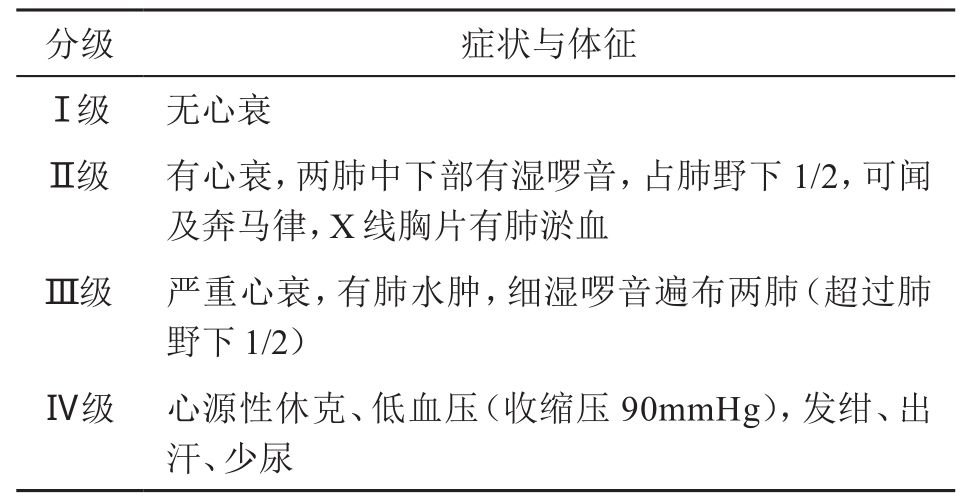
\includegraphics[width=3.21875in,height=1.66667in]{./images/Image00106.jpg}
\end{table}

\begin{table}[htbp]
\centering
\caption{急性左心衰的Forrester法分级}
\label{tab200-1}
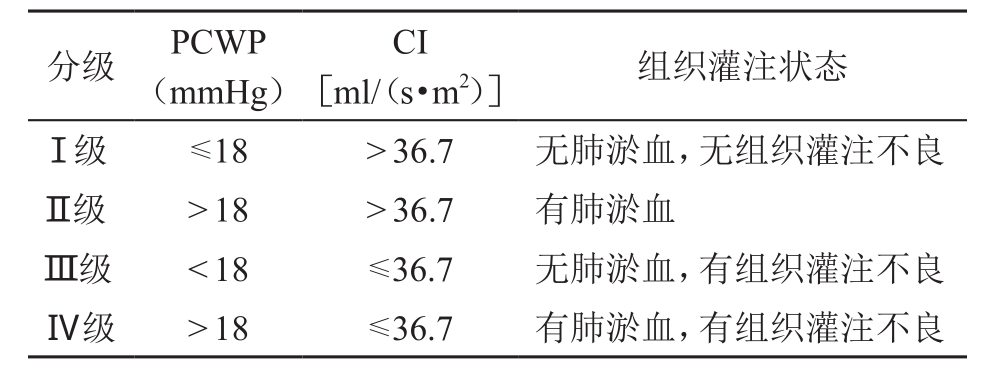
\includegraphics[width=3.27083in,height=1.22917in]{./images/Image00107.jpg}
\end{table}

\begin{table}[htbp]
\centering
\caption{急性左心衰的临床程度分级}
\label{tab300-1}
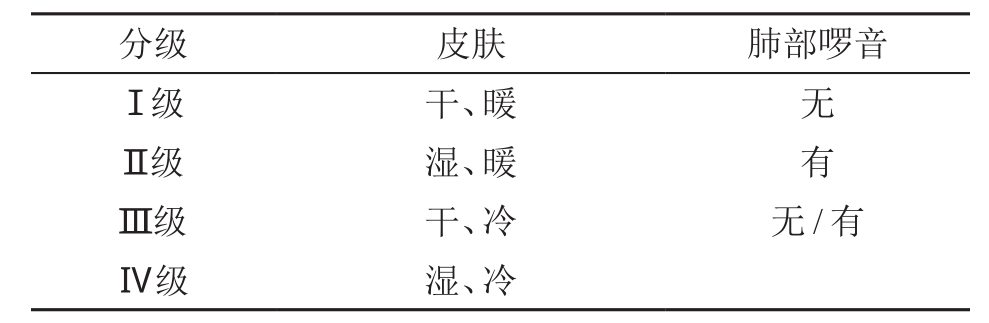
\includegraphics[width=3.28125in,height=1.0625in]{./images/Image00108.jpg}
\end{table}

\subsubsection{急性左心衰竭的监测方法}

\hypertarget{text00071.htmlux5cux23CHP3-2-5-4-5-1}{}
(一) 无创性监测(Ⅰ类、B级)

每个急性心衰患者均需应用床边监护仪持续测量体温、心率、呼吸频率、血压、心电图和血氧饱和度等。

\hypertarget{text00071.htmlux5cux23CHP3-2-5-4-5-2}{}
(二) 血流动力学监测

\subparagraph{适应证}

适用于血流动力学状态不稳定、病情严重且效果不理想的患者,如伴肺水肿(或)心源性休克的患者。

\subparagraph{方法}

①床边漂浮导管(Ⅰ类、B级):可用来测定主要的血流动力学指标如右心房压力(反映中心静脉压)、肺动脉压力(PAP)、PCWP,应用热稀释法可测定CO。可以持续监测上述各种指标的动态变化,酌情选择适当的药物,评估治疗的效果;②外周动脉插管(Ⅱa类,B级):可持续监测动脉血压,还可抽取动脉血样标本检查;③肺动脉插管(Ⅱa类,B级):不常规应用。对于病情复杂、合并心脏或肺部疾病者、其他检查难以确定时,可用来鉴别心源性或非心源性(例如肺源性)病因;对于病情极其严重,例如心源性休克的患者,可提供更多的血流动力学信息。

\subparagraph{注意 :}

①在二尖瓣狭窄、主动脉瓣反流、肺动脉闭塞病变以及左心室顺应性不良等情况下,PCWP往往不能准确反映左心室舒张末压。对于伴严重三尖瓣反流的患者,热稀释法测定CO也不可靠。②插入导管的各种并发症如感染、血栓形成或栓塞以及血管损伤等随导管留置时间延长而发生率明显增高。

\subsubsection{急性左心衰竭的诊断步骤}

可疑的急性左心衰竭患者应根据临床表现和辅助性检查作出诊断评估(附图1)。

\subsubsection{急性左心衰竭的鉴别诊断}

急性左心衰竭应与可引起明显呼吸困难的疾病如支气管哮喘发作和哮喘持续状态、急性大块肺栓塞、肺炎、严重的慢性阻塞性肺病(COPD)尤其伴感染等相鉴别,还应与其他原因所致的非心源性肺水肿(如急性呼吸窘迫综合征)以及非心源性休克等疾病相鉴别。

\subsubsection{急性右心衰竭的临床表现、诊断和鉴别诊断}

急性右心衰竭的诊断需根据病因。

\subparagraph{右心室梗死伴急性右心衰竭}

如心肌梗死时出现V\textsubscript{1} 、V\textsubscript{2}
导联ST段压低,应考虑右心室梗死,当然也有可能为后壁梗死,而非室间隔和心内膜下心肌缺血。下壁ST段抬高心肌梗死伴血流动力学障碍者应观察心电图V\textsubscript{4}
R导联,并作经胸壁超声心动图检查,后者发现右心室扩大伴活动减弱可以确诊右心室梗死。右心室梗死伴急性右心衰竭典型者可出现低血压、颈静脉显著充盈和肺部呼吸音清晰的三联症。

\subparagraph{急性大块肺栓塞伴急性右心衰竭}

典型表现为突发呼吸困难、剧烈胸痛、有濒死感,还有咳嗽、咯血痰、明显发绀、皮肤湿冷、休克和晕厥,伴颈静脉怒张、肝肿大、肺梗死区呼吸音减弱、肺动脉瓣区杂音。如有导致本病的基础病因及诱因,出现不明原因的发作性呼吸困难、发绀、休克,无心肺疾病史而突发的明显右心负荷过重和心衰,都应考虑肺栓塞。

\subparagraph{右侧心瓣膜病伴急性右心衰竭}

主要为右心衰竭的临床表现,有颈静脉充盈、下肢水肿、肝脏淤血等。

急性右心衰竭临床上应注意与急性心肌梗死、肺不张、急性呼吸窘迫综合征、主动脉夹层、心包压塞、心包缩窄等疾病相鉴别。

\subsubsection{急性心衰诊断和评估要点}

1.应根据基础心血管疾病
、诱因、临床表现(病史、症状和体征)以及各种检查(心电图、胸部X线检查、超声心动图和BNP/NT-proBNP)作出急性心衰的诊断,并做临床评估包括病情的分级、严重程度和预后。


\includegraphics[width=4.35417in,height=1.85417in]{./images/Image00109.jpg}

附图1 急性左心衰竭的诊断流程

2.常见的临床表现是急性左心衰竭所致的呼吸困难
,系由肺淤血所致,严重患者可出现急性肺水肿和心源性休克。

3.BNP/NT-proBNP作为心衰的生物学标志物,对急性左心衰竭诊断和鉴别诊断有肯定的价值,对患者的危险分层和预后评估有一定的临床价值。

4.急性左心衰竭病情严重程度分级有不同的方法
。Killip法适用于基础病因为急性心肌梗死的患者;Forrester法多用于心脏监护室、重症监护室及有血流动力学监测条件的场合;临床程度分级则可用于一般的门诊和住院患者。

5.急性右心衰竭主要常见病因为右心室梗死和急性大块肺栓塞
。根据病史、临床表现如突发的呼吸困难、低血压、颈静脉怒张等,结合心电图和超声心动图检查,可以作出诊断。

\subsection{急性心衰的治疗}

\subsubsection{治疗目标和处理流程}

\hypertarget{text00071.htmlux5cux23CHP3-2-5-5-1-1}{}
(一) 临床评估

对患者均应根据上述各种检查方法以及病情变化作出临床评估
,包括:①基础心血管疾病;②急性心衰发作的诱因;③病情的严重程度和分级,并估计预后;④治疗的效果。此种评估应多次和动态进行,以调整治疗方案。

\hypertarget{text00071.htmlux5cux23CHP3-2-5-5-1-2}{}
(二) 治疗目标

1.控制基础病因和矫治引起心衰的诱因
应用静脉和(或)口服降压药物以控制高血压;选择有效抗生素控制感染;积极治疗各种影响血流动力学的快速性或缓慢性心律失常;应用硝酸酯类药物改善心肌缺血。糖尿病伴血糖升高者应有效控制血糖水平,又要防止出现低血糖。对血红蛋白低于60g/L的严重贫血者,可输注浓缩红细胞悬液或全血。

2.缓解各种严重症状
①低氧血症和呼吸困难:采用不同方式吸氧,包括鼻导管吸氧、面罩吸氧以及无创或气管插管的呼吸机辅助通气治疗;②胸痛和焦虑:应用吗啡;③呼吸道痉挛:应用支气管解痉药物;④淤血症状:利尿剂有助于减轻肺淤血和肺水肿,亦可缓解呼吸困难。

3.稳定血流动力学状态 ,维持收缩压≥90mmHg
纠正和防止低血压可应用各种正性肌力药物。血压过高者的降压治疗可选择血管扩张药物。

4.纠正水、电解质紊乱和维持酸碱平衡
静脉应用袢利尿剂应注意补钾和保钾治疗;血容量不足、外周循环障碍、少尿或伴肾功能减退患者要防止高钾血症。低钠血症者应适当进食咸菜等补充钠盐,严重低钠血症(<
110mmol/L)者应根据计算所得的缺钠量,静脉给予高张钠盐如3\%~6\%氯化钠溶液,先补充缺钠量的1/3~1/2,而后酌情继续补充。出现酸碱平衡失调时,应及时予以纠正。

5.保护重要脏器如肺、肾、肝和大脑,防止功能损害。

6.降低死亡危险,改善近期和远期预后。

\subsubsection{急性左心衰竭的处理流程}

急性左心衰竭确诊后即按附图2的流程处理。初始治疗后症状未获明显改善或病情严重者应作进一步治疗。血管活性药物可按附表4所列方法选择应用,其应用方法参见下文“四、急性左心衰竭的药物治疗”。

附表4 急性左心衰竭的血管活性药物的选择应用

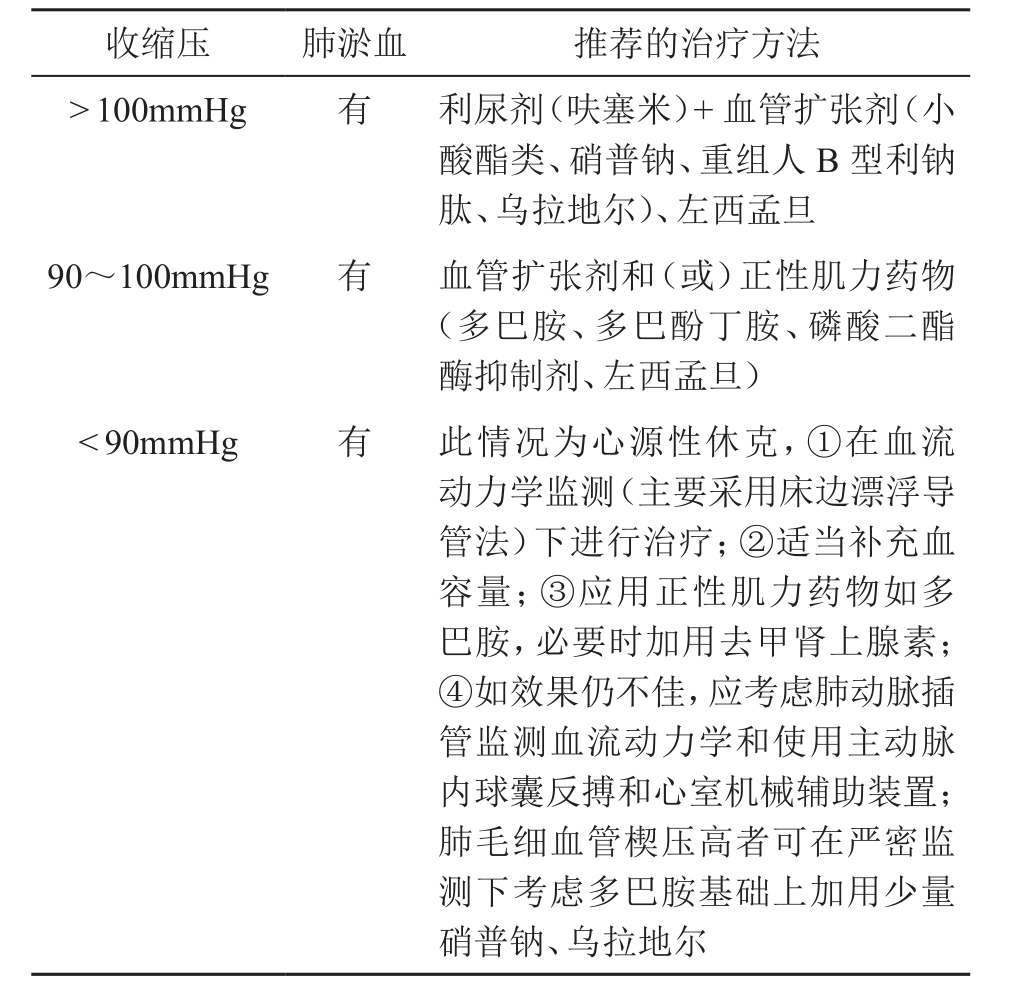
\includegraphics[width=3.35417in,height=3.29167in]{./images/Image00110.jpg}

\subsubsection{急性左心衰竭的一般处理}

\subparagraph{体位}

静息时明显呼吸困难者应半卧位或端坐位,双腿下垂以减少回心血量,降低心脏前负荷。

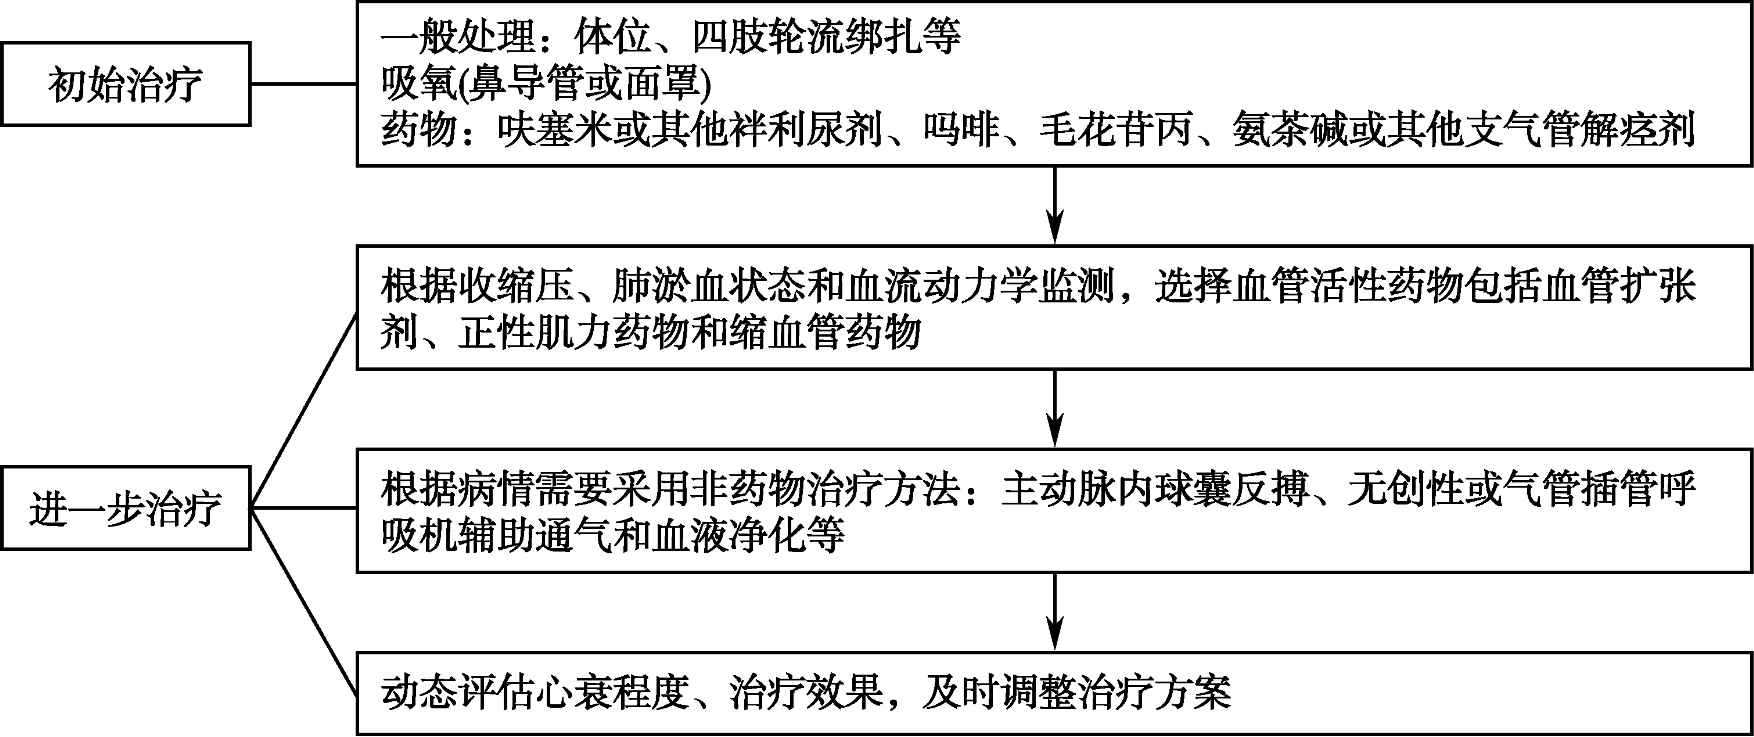
\includegraphics[width=5.03125in,height=2.10417in]{./images/Image00111.jpg}

附图2 急性左心衰竭的处理流程

\subparagraph{四肢交换加压}

四肢轮流绑扎止血带或血压计袖带,通常同一时间只绑扎三肢,每隔15~20分钟轮流放松一肢。血压计袖带的充气压力应较舒张压低10mmHg,使动脉血流仍可顺利通过,而静脉血回流受阻。此法可降低前负荷,减轻肺淤血和肺水肿。

\subparagraph{吸氧}

适用于低氧血症和呼吸困难明显(尤其指端血氧饱和度<
90\%)的患者。应尽早采用,使患者SaO\textsubscript{2}
≥95\%(伴COPD者SaO\textsubscript{2} >
90\%)。可采用不同的方式:①鼻导管吸氧:低氧流量(1~2L/min)开始,如仅为低氧血症,动脉血气分析未见CO\textsubscript{2}
潴留,可采用高流量给氧6~8L/min。酒精吸氧可使肺泡内的泡沫表面张力减低而破裂,改善肺泡的通气。方法是在氧气通过的湿化瓶中加50\%~70\%酒精或有机硅消泡剂,用于肺水肿患者。②面罩吸氧:适用于伴呼吸性碱中毒患者。必要时还可采用无创性或气管插管呼吸机辅助通气治疗。

\subparagraph{做好救治的准备工作}

至少开放2根静脉通道,并保持通畅。必要时可采用深静脉穿刺置管,以随时满足用药的需要。血管活性药物一般应用微量泵泵入,以维持稳定的速度和正确的剂量。固定和维护好漂浮导管、深静脉置管、心电监护的电极和导联线、鼻导管或面罩、导尿管以及指端无创血氧仪测定电极等。保持室内适宜的温度、湿度,灯光柔和,环境幽静。

\subparagraph{饮食}

进易消化食物,避免一次大量进食,不要饱餐。在总量控制下,可少量多餐(每天6~8次)。应用袢利尿剂情况下不要过分限制钠盐摄入量,以避免低钠血症,导致低血压。利尿剂应用时间较长的患者要补充多种维生素和微量元素。

\subparagraph{出入量管理}

肺淤血、体循环淤血及水肿明显者应严格限制饮水量和静脉输液速度,对无明显低血容量因素(大出血、严重脱水、大汗淋漓等)者的每天摄入液体量一般宜在1500ml以内,不要超过2000ml。保持每天水出入量负平衡约500ml/d,以减少水钠潴留和缓解症状。3~5天后,如淤血、水肿明显消退,应减少水负平衡,逐渐过渡到出入水量大体平衡。在水负平衡下应注意防止发生低血容量、低血钾和低血钠等。

\subsubsection{急性左心衰竭的药物治疗}

\hypertarget{text00071.htmlux5cux23CHP3-2-5-5-4-1}{}
(一) 镇静剂

主要应用吗啡(Ⅱa类,C级):用法为2.5~5.0mg静脉缓慢注射,亦可皮下或肌肉注射。伴CO\textsubscript{2}
潴留者则不宜应用,可产生呼吸抑制而加重CO\textsubscript{2}
潴留;也不宜应用大剂量,可促使内源性组胺释放,使外周血管扩张导致血压下降。应密切观察疗效和呼吸抑制的不良反应。伴明显和持续低血压、休克、意识障碍、COPD等患者禁忌使用。老年患者慎用或减量。亦可应用哌替啶50~100mg肌肉注射。

\hypertarget{text00071.htmlux5cux23CHP3-2-5-5-4-2}{}
(二) 支气管解痉剂(Ⅱa类,C级)

一般应用氨茶碱0.125~0.25g以葡萄糖水稀释后静脉推注(10分钟),4~6小时后可重复一次;或以0.25~0.5mg/(kg•h)静脉滴注。亦可应用二羟丙茶碱0.25~0.5g静脉滴注,速度为25~50mg/h。此类药物不宜用于冠心病如急性心肌梗死或不稳定性心绞痛所致的急性心衰患者(Ⅱb类,C级),不可用于伴心动过速或心律失常的患者。

\hypertarget{text00071.htmlux5cux23CHP3-2-5-5-4-3}{}
(三) 利尿剂(Ⅰ类,B级)

\subparagraph{应用指征和作用机制}

适用于急性心衰伴肺循环和(或)体循环明显淤血以及容量负荷过重的患者。作用于肾小管亨利袢的利尿剂如呋塞米、托塞米、布美他尼静脉应用可以在短时间里迅速降低容量负荷,应列为首选。噻嗪类利尿剂、保钾利尿剂(阿米洛利、螺内酯)等仅作为袢利尿剂的辅助或替代药物,或在需要时作为联合用药。临床上利尿剂应用十分普遍,但并无大样本随机对照试验进行评估。

\subparagraph{药物种类和用法}

应采用静脉利尿制剂,首选呋塞米,先静脉注射20~40mg,继以静脉滴注5~40mg/h,其总剂量在起初6小时不超过80mg,起初24小时不超过200mg。亦可应用托塞米10~20mg或依那尼酸25~50mg静脉注射。袢利尿剂效果不佳、加大剂量仍未见良好反应以及容量负荷过重的急性心衰患者,应加用噻嗪类和(或)醛固酮受体拮抗剂:氢氯噻嗪25~50mg、每日2次,或螺内酯20~40mg/d。临床研究表明,利尿剂低剂量联合应用,其疗效优于单一利尿剂的大剂量,且不良反应也更少。

\subparagraph{注意事项}

①伴低血压(收缩压<
90mmHg)、严重低钾血症或酸中毒患者不宜应用,且对利尿剂反应甚差;②大剂量和较长时间的应用可发生低血容量和低钾血症、低钠血症,且增加其他药物如血管紧张素转化酶抑制剂(ACEI)、血管紧张素Ⅱ受体拮抗剂(ARB)或血管扩张剂引起低血压的可能性;③应用过程中应检测尿量,并根据尿量和症状的改善状况调整剂量。

\hypertarget{text00071.htmlux5cux23CHP3-2-5-5-4-4}{}
(四) 血管扩张药物

\subparagraph{应用指征}

此类药可应用于急性心衰早期阶段。收缩压水平是评估此类药是否适宜的重要指标。收缩压>
110mmHg的急性心衰患者通常可以安全使用;收缩压在90~110mmHg之间的患者应谨慎使用;而收缩压<
90mmHg的患者则禁忌使用。

\subparagraph{主要作用机制}

可降低左、右心室充盈压和全身血管阻力,也使收缩压降低,从而减轻心脏负荷,缓解呼吸困难。如舒张压在60mmHg以上,通常冠状动脉血流可维持正常。对于急性心衰,包括合并急性冠状动脉综合征的患者,此类药在缓解肺淤血和肺水肿的同时不会影响心排血量,也不会增加心肌耗氧量。

\subparagraph{药物种类和用法}

主要有硝酸酯类、硝普钠、重组人BNP(rhBNP)、乌拉地尔、酚妥拉明,但钙拮抗剂不推荐用于急性心衰的治疗。

\hypertarget{text00071.htmlux5cux23CHP3-2-5-5-4-4-3-1}{}
(1) 硝酸酯类药物(Ⅰ类、B剂):

急性心衰时此类药在不减少每搏心输出量和不增加心肌氧耗情况下能减轻肺淤血,特别适用于急性冠状动脉综合征伴心衰的患者。临床研究已证实,硝酸酯类静脉制剂与呋塞米合用治疗急性心衰有效;还证实应用血流动力学可耐受的最大剂量并联合小剂量呋塞米的疗效优于单纯大剂量的利尿剂。

静脉应用硝酸酯类药物应十分小心滴定剂量,经常测量血压,防止血压过度下降。硝酸甘油静脉滴注起始剂量5~10μg/min,每5~10分钟递增5~10μg/min,最大剂量100~200μg/min;亦可每10~15分钟喷雾一次(400μg),或舌下含服0.3~0.6mg/次。硝酸异山梨酯静脉滴注剂量5~10mg/h,亦可舌下含服2.5mg/次。

\hypertarget{text00071.htmlux5cux23CHP3-2-5-5-4-4-3-2}{}
(2) 硝普钠(Ⅰ类、C级):

适用于严重心衰、原有后负荷增加以及伴心源性休克患者。临床应用宜从小剂量10μg/min开始,可酌情逐渐增加剂量至50~250μg/min,静脉滴注,疗程不要超过72小时。由于其强效降压作用,应用过程中要密切监测血压,根据血压调整合适的维持剂量。停药应逐渐减量,并加用口服血管扩张剂,以避免反跳现象。

\hypertarget{text00071.htmlux5cux23CHP3-2-5-5-4-4-3-3}{}
(3) rhBNP(Ⅱa类,B级):

该药近几年刚应用于临床,属内源性激素物质,与人体内产生的BNP完全相同。国内制剂商品名为新活素,国外同类药名为奈西立肽(nesiritide)。其主要药理作用是扩张静脉和动脉(包括冠状动脉),从而降低前、后负荷,在无直接正性肌力作用情况下增加CO,故将其归类为血管扩张剂。实际该药并非单纯的血管扩张剂,而是一种兼具多重作用的治疗药物;可以促进钠的排泄,有一定的利尿作用;还可抑制RAAS和较高神经系统,阻滞急性心衰演变中的恶性循环。该药临床试验的结果尚不一致。晚近的两项研究(VMAC和PROACTION)表明,该药的应用可以带来临床和血流动力学的改善,推荐应用于急性失代偿心衰。国内一项Ⅱ期临床研究提示,rhBNP较硝酸甘油静脉制剂能够显著降低PCWP,缓解患者的呼吸困难。应用方法:先给予负荷剂量1.500μg/kg,静脉缓慢推注,继以0.0075~0.0150μg/(kg•min)静脉滴注;也可不用负荷剂量而直接静脉滴注。疗程一般3天,不超过7天。

\hypertarget{text00071.htmlux5cux23CHP3-2-5-5-4-4-3-4}{}
(4) 乌拉地尔(Ⅱa类,C级):

该药具有外周和中枢双重扩血管作用,可有效降低血管阻力,降低后负荷,增加心输出量,但不影响心率,从而减少心肌耗氧量。适用于高血压性心脏病、缺血性心肌病(包括急性心肌梗死)和扩张型心肌病引起的急性左心衰;可用于CO降低、PCWP
>
18mmHg的患者。通常静脉滴注100~400μg/min,可逐渐增加剂量,并根据血压和临床状况予以调整。伴严重高血压者可缓慢静脉注射12.5~25.0mg。

\hypertarget{text00071.htmlux5cux23CHP3-2-5-5-4-4-3-5}{}
(5) ACEI:

该药在急性心衰中的应用仍有诸多争议。急性心衰的急性期、病情尚未稳定的患者不宜应用(Ⅱb类,C级)。急性心肌梗死后的急性心衰可以试用(Ⅱa类,C级),但须避免静脉应用,口服起始剂量宜小。在急性期病情稳定48小时后逐渐加量(Ⅰ类,A级),疗程至少6周,不能耐受ACEI者可以应用ARB。

\subparagraph{注意事项}

下列情况下禁用血管扩张药物:①收缩压<
90mmHg,或持续低血压并伴症状尤其有肾功能不全的患者,以避免重要脏器灌注减少;②严重阻塞性心瓣膜疾病患者,例如主动脉瓣狭窄,有可能出现显著的低血压;二尖瓣狭窄患者也不宜应用,有可能造成CO明显降低;③梗阻性肥厚型心肌病。

\hypertarget{text00071.htmlux5cux23CHP3-2-5-5-4-5}{}
(五) 正性肌力药物

1.应用指征和作用机制
此类药物适用于低心排血量综合征,如伴症状性低血压或CO降低伴有循环淤血的患者,可缓解组织低灌注所致的症状,保证重要脏器的血流供应。血压较低和对血管扩张药物及利尿剂不耐受或反应不佳的患者尤其有效。

2.药物种类和用法如下。

(1) 洋地黄类(Ⅱa类,C级)
此类药物能轻度增加CO和降低左心室充盈压;对急性左心衰竭患者的治疗有一定帮助。一般应用毛花苷丙0.2~0.4mg缓慢静脉注射,2~4小时后可以再用0.2mg,伴快速心室率的房颤患者可酌情适当增加剂量。

(2)
多巴胺(Ⅱa类,C级):250~500μg/min静脉滴注。此药应用个体差异较大,一般从小剂量开始,逐渐增加剂量,短期应用。

(3)
多巴酚丁胺(Ⅱa类,C级):该药短期应用可以缓解症状,但并无临床证据表明对降低病死率有益。用法:100~250μg/min静脉滴注。使用时注意监测血压,常见不良反应有心律失常、心动过速,偶尔可因加重心肌缺血而出现胸痛。正在应用β受体阻滞剂的患者不推荐应用多巴酚丁胺和多巴胺。

(4)
磷酸二酯酶抑制剂(Ⅱb类,C级):米力农,首剂25~50μg/kg静脉注射(大于10分钟),继以0.25~0.50μg
/
(kg•min)静脉滴注。氨力农首剂0.5~0.75mg/kg静脉注射(大于10分钟),继以5~10μg/(kg•min)静脉滴注。常见不良反应有低血压和心律失常。

(5)
左西孟旦(Ⅱa类,B级):这是一种钙增敏剂,通过结合于心肌细胞上的肌钙蛋白C促进心肌收缩,还通过介导ATP敏感的钾通道而发挥血管舒张作用和轻度抑制磷酸二酯酶的效应。其正性肌力作用独立于β肾上腺素能刺激,可用于正接受β受体阻滞剂治疗的患者。临床研究表明,急性心衰患者应用本药静脉滴注可明显增加CO和每搏量,降低PCWP、全身血管阻力和肺血管阻力;冠心病患者不会增加病死率。用法:首剂12~24μg/kg静脉注射(大于10分钟),继以0.1μg/(kg•min)静脉滴注,可酌情减半或加倍。对于收缩压<
100mmHg的患者,不需要负荷剂量,可直接用维持剂量,以防止发生低血压。

3.注意事项
急性心衰患者应用此类药需全面权衡:①是否用药不能仅依赖1、2次血压测量的数值,必须综合评价临床状况,如是否伴组织低灌注的表现;②血压降低伴低CO或低灌注时应尽早使用,而当器官灌注恢复和(或)循环淤血减轻时则应尽快停用;③药物的剂量和静脉滴注速度应根据患者的临床反应作调整,强调个体化的治疗;④此类药可即刻改善急性心衰患者的血流动力学和临床状态,但也有可能促进和诱发一些不良的病理生理反应,甚至导致心肌损伤和靶器官损害,必须警惕;⑤血压正常又无器官和组织灌注不足的急性心衰患者不宜使用。

\subsubsection{急性右心衰竭的治疗}

\hypertarget{text00071.htmlux5cux23CHP3-2-5-5-5-1}{}
(一) 右心室梗死伴急性右心衰竭

1.扩容治疗
如存在心源性休克,在监测中心静脉压的基础上首要治疗是大量补液,可应用706代血浆、低分子右旋糖酐或生理盐水20ml/min静脉滴注,直至PCWP上升至15~18mmHg,血压回升和低灌注症状改善。24小时的输液量大约在3500~5000ml。对于充分扩容而血压仍低者,可给予多巴酚丁胺或多巴胺。如在补液过程中出现左心衰竭,应立即停止补液。此时若动脉血压不低,可小心给予血管扩张药。

2.禁用利尿剂
、吗啡和硝酸甘油等血管扩张剂,以避免进一步降低右心室充盈压。

3.如右心室梗死同时合并广泛左心室梗死
,则不宜盲目扩容,防止造成急性肺水肿。如存在严重左心室功能障碍和PCWP升高,不宜使用硝普钠,应考虑主动脉内球囊反搏(IABP)治疗。

\hypertarget{text00071.htmlux5cux23CHP3-2-5-5-5-2}{}
(二) 急性大块肺栓塞所致急性右心衰竭

\subparagraph{止痛}

吗啡或哌替啶。

\subparagraph{吸氧}

鼻导管或面罩给氧6~8L/min。

\subparagraph{溶栓治疗}

常用尿激酶或人重组组织型纤溶酶原激活剂(rt-PA)。停药后应继续肝素治疗。用药期间监测凝血酶原时间,使之延长至正常对照的1.5~2.0倍。持续滴注5~7天,停药后改用华法林口服数月。

\subparagraph{经内科治疗无效的危重患者}

(如休克),若经肺动脉造影证实为肺总动脉或其较大分支内栓塞,可作介入治疗,必要时可在体外循环下紧急早期切开肺动脉摘除栓子。

\hypertarget{text00071.htmlux5cux23CHP3-2-5-5-5-3}{}
(三) 右侧心瓣膜病所致急性右心衰竭

右心衰竭的治疗主要应用利尿剂
,以减轻水肿;但要防止过度利尿造成心排血量减少。此外,对基础心脏病如肺动脉高压、肺动脉狭窄以及合并肺动脉瓣或三尖瓣关闭不全、感染性心内膜炎等,按相应的指南予以治疗。肺源性心脏病合并的心衰属右心衰竭,其急性加重可视为一种特殊类型的急性右心衰竭,亦应按该病的相应指南治疗。

\subsubsection{非药物治疗}

\hypertarget{text00071.htmlux5cux23CHP3-2-5-5-6-1}{}
(一) 主动脉内球囊反搏(IABP)

临床研究表明,这是一种有效改善心肌灌注同时又降低心肌耗氧量和增加CO的治疗手段。

\subparagraph{IABP的适应证(Ⅰ类、B级)}

①急性心肌梗死或严重心肌缺血并发心源性休克,且不能由药物治疗纠正;②伴血流动力学障碍的严重冠心病(如急性心肌梗死伴机械并发症);③心肌缺血伴顽固性肺水肿。

\subparagraph{IABP的禁忌证}

①存在严重的外周血管疾病;②主动脉瘤;③主动脉瓣关闭不全;④活动性出血或其他抗凝禁忌证;⑤严重血小板缺乏。

\subparagraph{IABP的撤除}

急性心衰患者的血流动力学稳定后可撤除IABP,撤除的参考指征为:①CI >
2.5L/(min•m\textsuperscript{2} );②尿量>
1ml/(kg•h);③血管活性药物用量逐渐减少,而同时血压恢复较好;④呼吸稳定,动脉血气分析各项指标正常;⑤降低反搏频率时血流动力学参数仍然稳定。

\hypertarget{text00071.htmlux5cux23CHP3-2-5-5-6-2}{}
(二) 机械通气

急性心衰患者行机械通气的指征
:①出现心跳呼吸骤停而进行心肺复苏时;②合并Ⅰ型或Ⅱ型呼吸衰竭。机械通气的方式有下列两种。

\subparagraph{无创呼吸机辅助通气}

这是一种无需气管插管、经口/鼻面罩给患者供氧、由患者自主呼吸触发的机械通气治疗。分为持续气道正压通气(CPAP)和双相间歇气道正压通气(BiPAP)两种模式。①作用机制:通过气道正压通气可改善患者的通气状况,减轻肺水肿,纠正缺氧和CO\textsubscript{2}
潴留,从而缓解Ⅰ型或Ⅱ型呼吸衰竭。②适用对象:Ⅰ型或Ⅱ型呼吸衰竭患者经常规吸氧和药物治疗仍不能纠正时应及早应用。主要用于呼吸频率≤25次/分、能配合呼吸机通气的早期呼吸衰竭患者。在下列情况下应用受限:不能耐受和合作的患者、有严重认知障碍和焦虑的患者、呼吸急促(频率>
25次/分)、呼吸微弱和呼吸道分泌物多的患者。

\subparagraph{气管插管和人工机械通气}

应用指征为心肺复苏时、严重呼吸衰竭经常规治疗不能改善者,尤其是出现明显呼吸性和代谢性酸中毒并影响到意识状态的患者。

\hypertarget{text00071.htmlux5cux23CHP3-2-5-5-6-3}{}
(三) 血液净化治疗(Ⅱa类,B级)

\subparagraph{机制}

此法不仅可维持水、电解质和酸碱平衡,稳定内环境,还可清除尿毒症毒素(肌酐、尿素、尿酸等)、细胞因子、炎症介质以及心脏抑制因子等。治疗中的物质交换可通过血液滤过(超滤)、血液透析、连续血液净化和血液灌流等来完成。

\subparagraph{适应证}

本法对急性心衰有益,但并非常规应用的手段。出现下列情况之一可以考虑采用:①高容量负荷如肺水肿或严重的外周组织水肿,且对袢利尿剂和噻嗪类利尿剂抵抗;②低钠血症(血钠<
110mmol/L)且有相应的临床症状如神志障碍、肌张力减退、腱反射减弱或消失、呕吐以及肺水肿等,在上述两种情况应用单纯血液滤过即可;③肾功能进行性减退,血肌酐>
500μmol/L或符合急性血液透析指征的其他情况。

\subparagraph{不良反应和处理}

建立体外循环的血液净化均存在与体外循环相关的不良反应如生物不相容、出血、凝血、血管通路相关并发症、感染、机器相关并发症等。应避免出现新的内环境紊乱,连续血液净化治疗时应注意热量及蛋白的丢失。

\hypertarget{text00071.htmlux5cux23CHP3-2-5-5-6-4}{}
(四) 心室机械辅助装置(Ⅱa类,B级)

急性心衰经常规药物治疗无明显改善时,有条件的可应用此种技术。此类装置有:体外模式人工肺氧合器(ECMO)、心室辅助泵(如可置入式电动左心辅助泵、全人工心脏)。根据急性心衰的不同类型,可选择应用心室辅助装置,在积极纠治基础心脏病的前提下,短期辅助心脏功能,可作为心脏移植或心肺移植的过渡。ECMO可以部分或全部代替心肺功能。临床研究表明,短期循环呼吸支持(如应用ECMO)可以明显改善预后。

\hypertarget{text00071.htmlux5cux23CHP3-2-5-5-6-5}{}
(五) 外科手术

\subparagraph{冠心病}

\hypertarget{text00071.htmlux5cux23CHP3-2-5-5-6-5-1-1}{}
(1) 不稳定性心绞痛或心肌梗死并发心源性休克:

经冠状动脉造影证实为严重左主干或多支血管病变,并在确认冠状动脉支架术和溶栓治疗无效的前提下,可进行冠状动脉旁路移植术,能够明显改善心衰。经积极的抗急性心衰药物治疗,并在机械通气、IABP等辅助下,甚至在体外循环支持下应立即急诊手术。

\hypertarget{text00071.htmlux5cux23CHP3-2-5-5-6-5-1-2}{}
(2) 心肌梗死后机械并发症:

①心室游离壁破裂:心肌梗死后游离壁破裂的发生率约为0.8\%~6.2\%,可导致心脏压塞和电机械分离,猝死在数分钟内即出现;亚急性破裂并发心源性休克则为手术提供了机会,确诊后经心包穿刺减压、补液和应用药物维持下,宜立即手术。②室间隔穿孔:心肌梗死后本病发生率为1\%~2\%,多在1~5天内。最常见前壁心肌梗死,多见于老年、女性,院内病死率可达81\%(SHOCK研究)。直接的诊断依据主要依靠超声心动图、心导管及左心室造影检查,可证实穿孔部位、分流量以及是否合并二尖瓣关闭不全。在药物和非药物积极治疗下行冠状动脉造影。确诊后若经药物治疗可使病情稳定,尽量争取4周后手术治疗;若药物治疗(包括IABP)不能使病情稳定,应早期手术修补,同期进行冠状动脉旁路移植术。对不合并休克的患者,血管扩张剂如硝酸甘油或硝普钠可使病情有所改善;对合并心源性休克的患者,IABP对造影和手术准备可提供最有效的血流动力学支持。急诊手术对大的室间隔穿孔合并心源性休克的患者是使之存活的唯一方法,但手术病死率很高。对血流动力学稳定的患者(除非症状不显著的小缺损)也多主张早期手术治疗,因破裂缺损可能扩大。但最佳手术时机目前并未达成共识。在急性期,因坏死心肌松脆,手术有技术困难。近年来,经皮室间隔缺损封堵术用于部分经选择的患者,但尚有待进一步积累经验,以确定其应用价值。③重度二尖瓣关闭不全:本病在急性心肌梗死伴心源性休克患者中约占10\%,多出现在2~7天。完全性乳头肌断裂者多在24小时内死亡,而乳头肌功能不全者较为多见,且预后较好。超声心动图可确诊并测反流量和左心室功能。应在IABP支持下行冠状动脉造影。出现肺水肿者应立即作瓣膜修补术或瓣膜置换术,并同期行冠状动脉旁路移植术。

\subparagraph{心瓣膜疾病}

除缺血性乳头肌功能不全外,因黏液性腱索断裂、心内膜炎、创伤等所致的急性二尖瓣关闭不全以及因感染性心内膜炎、主动脉夹层、胸部闭合伤等所致的急性主动脉瓣关闭不全均应尽早手术干预。此外,主动脉瓣或二尖瓣的严重狭窄以及联合心瓣膜病的心功能失代偿期也需要尽早手术。人工瓣膜血栓形成或瓣膜失功能所致的急性心衰病死率极高,超声心动图(必要时应用经食管超声心动图)可明确诊断,均应手术,尤其左心系统的血栓应立即手术。

\subparagraph{急性主动脉夹层}

本病(尤其Ⅰ型)因高血压危象和主动脉瓣反流可出现急性心衰。超声心动图一旦明确主动脉瓣反流,应立即手术。

\subparagraph{其他疾病}

主动脉窦瘤破裂、心脏内肿瘤(如左心房黏液瘤)以及心脏内巨大血栓形成(在左心房或肺动脉)等均会造成瓣膜反流或流出道梗阻,可引起急性心衰,需要立即手术。心脏外科手术中,心肌保护不良、心脏阻断时间延长或反复多次阻断、心脏畸形纠正不彻底、心脏移植供心缺血时间过长以及术后心包压塞等均可造成严重低心排综合征,需要给予积极的药物和非药物(包括IABP和ECMO)治疗,甚至再次手术。各种心导管检查和介入治疗并发症亦可导致急性心衰,其所致的急性心肌梗死、冠状动脉损伤、二尖瓣球囊扩张术后重度反流、封堵器脱落梗阻、心脏破损出血以及心包压塞均需要紧急手术。

\subsubsection{急性心衰处理要点}

1.确诊后即应采用规范的处理流程 。先进行初始治疗,继以进一步治疗。

2.初始治疗包括经鼻导管或面罩吸氧
,静脉给予吗啡、袢利尿剂(如呋塞米)、毛花苷丙、氨茶碱(或二羟丙茶碱)等。

3.初始治疗仍不能缓解病情的严重患者应做进一步治疗
,可根据收缩压和肺淤血状况选择应用血管活性药物包括正性肌力药、血管扩张药和缩血管药。

4.病情严重或有血压持续降低(<
90mmHg)甚至心源性休克者,应在血流动力学监测下进行治疗,并酌情采用各种非药物治疗方法包括IABP、机械通气支持、血液净化、心室机械辅助装置以及外科手术。

5.BNP/NT-proBNP的动态测定有助于指导急性心衰的治疗,其水平在治疗后仍高居不下者,提示预后差,需进一步加强治疗;治疗后其水平降低且降幅>
30\%,提示治疗有效,预后较好。

6.要及时矫正基础心血管疾病,控制和消除各种诱因。

\subsection{急性心衰的基础疾病处理}

\subsubsection{缺血性心脏病所致的急性心衰}

1.缺血性心脏病是 40岁以上人群心衰的最常见病因
。通过询问病史和心血管危险因素、心电图和心肌损伤标志物等检查,特别是心电图和心肌血清标志物的动态变化多数可以明确缺血性心脏病的诊断。超声心动图检查有助于了解和评价心脏的结构变化和功能。

2.针对缺血性心脏病的病因治疗
①抗血小板治疗:对于合并急性心肌梗死和不稳定心绞痛的患者,要给予阿司匹林和氯吡格雷等强化抗血小板治疗;而对于无急性心肌梗死和不稳定性心绞痛的患者,口服阿司匹林即可。②抗凝治疗:对于急性心肌梗死和不稳定性心绞痛等患者可根据相应指南给予低分子肝素或普通肝素等抗凝治疗。③改善心肌供血和减少心肌耗氧的治疗,应给予口服和静脉硝酸酯类药物。④他汀类药物治疗。⑤对于因心肌缺血发作而诱发和加重的急性心衰(主要表现有胸痛、胸闷等症状,心电图有动态的缺血性ST-T改变),如果患者血压偏高、心率增快,可在积极控制心衰的基础治疗上慎重应用口服甚至静脉注射β受体阻滞剂,有利于减慢心率和降低血压,从而减少心肌耗氧量,改善心肌缺血和心功能。⑥对于ST段抬高急性心肌梗死,若在溶栓和急诊介入治疗时间窗内就诊并有溶栓和介入治疗指征,在评价病情和治疗风险后,如在技术上能够迅速完成同时患者家属充分理解,则可予急诊介入治疗或静脉溶栓治疗。但此时介入治疗风险较大,必要时在应用IABP支持下行介入治疗更安全。及早开通梗死相关冠状动脉可挽救濒死心肌、缩小梗死面积,有利于急性心衰的控制。对于已经出现急性肺水肿和明确的Ⅰ或Ⅱ型呼吸衰竭者则首先纠正肺水肿和呼吸衰竭。⑦合并低血压和休克者,如有条件可积极给予IABP或ECMO等机械辅助支持治疗,有助于提高抢救成功率。⑧除急诊介入治疗外,冠状动脉造影和血运重建治疗应在急性心衰得到有效缓解后进行。

\subsubsection{高血压所致的急性心衰}

其临床特点是高血压(> 180/120mmHg),心衰发展迅速,CI通常正常,PCWP >
18mmHg,X线胸片正常或呈间质性肺水肿。此种状态属高血压急症,应把握适当的降压速度。慢性高血压患者因血压自动调节功能受损,快速降压可导致心、脑、肾等重要脏器供血不足;急进型恶性高血压患者因其小动脉狭窄,已存在局部供血不足,快速降压会加重脏器缺血。如急性心衰病情较轻,可在24~48小时内逐渐降压;病情重、伴肺水肿患者应在1小时内将平均动脉压较治疗前降低≤25\%,2~6小时降至160/100~110mmHg,24~48小时内使血压逐渐降至正常。优先考虑静脉给予硝酸甘油,亦可应用硝普钠。呋塞米等袢利尿剂静脉给予能起辅助降压之效。乌拉地尔适用于基础心率很快、应用硝酸甘油或硝普钠后心率迅速增加而不能耐受的患者。

\subsubsection{心瓣膜病所致的急性心衰}

任何内科治疗和药物均不可能消除或缓解心瓣膜病变及其造成的器质性损害。此种损害可促发心肌重构,最终导致心衰。在疾病逐渐进展过程中,一些因素尤其伴快速心室率的房颤、感染、体力负荷加重等均可诱发心衰的失代偿或发生急性心衰。因此,对于此类患者早期采用介入或外科手术矫治是预防心衰的唯一途径,部分无症状的心瓣膜病患者亦应积极考虑采用,以从根本上改善其预后。

伴发急性心衰的患者,原则上应积极采取本指南所列的各种治疗举措,力求稳定病情,缓解症状,以便尽快进行心瓣膜的矫治术。已经发生心衰的患者,均必须进行心瓣膜矫治术,不应迟疑。反复的心衰发作不仅加重病情,也会增加手术的风险,并影响术后心功能的改善程度。

风湿性二尖瓣狭窄所致的急性肺水肿常由快速心室率的房颤诱发,在农村地区仍较常见。有效地控制房颤的心室率对成功治疗急性心衰极其重要。可应用毛花苷丙0.4~0.6mg缓慢静脉注射,必要时1~2小时后重复一次,剂量减半。效果不理想者,可加用静脉β受体阻滞剂,宜从小剂量开始(普通剂量之半),酌情增加剂量,直至心室率得到有效控制。此外,还可静脉使用胺碘酮。药物无效者可考虑电复律。一旦急性心衰得到控制,病情缓解,应尽早考虑介入术或外科手术,以解除瓣膜狭窄。

\subsubsection{非心脏手术围术期发生的急性心衰}

这是一种较为常见的急性心衰类型,也是引起围术期患者死亡的原因之一。

\subparagraph{评估患者的风险 ,作出危险分层}

根据可能发生急性心衰的风险,术前可作出危险分层。①高危:不稳定性心绞痛、急性心肌梗死(7天以内)、新近发生心肌梗死(7天~1个月)、失代偿性心衰、严重或高危心律失常、严重心瓣膜病以及高血压Ⅲ级(>
180/110mmHg)。②中危:缺血性心脏病史、心衰或心衰失代偿史、脑血管病(短暂性脑缺血发作、脑卒中)、糖尿病以及肾功能不全。③低危:年龄>
70岁、心电图异常(左心室肥厚、完全性左束支传导阻滞、非特异性ST-T改变)、非窦性心律以及未控制的高血压。高危者应推迟或取消手术。中、低危者术前应做充分的预防治疗。多个低危因素并存,手术风险也会增加。

\subparagraph{评估手术类型的风险}

不同类型的手术对心脏的危险不同。对于风险较高的手术,术前要做充分的预防治疗。①心脏危险>
5\%的手术:主动脉和其他主要血管的手术、外周血管手术;②心脏危险1\%~5\%的手术:腹腔内手术、胸腔内手术、头颈部手术、颈动脉内膜切除术、整形手术、前列腺手术;③心脏危险<
1\%的手术:内镜手术、皮肤浅层手术、白内障手术、乳腺手术、门诊手术。

\subparagraph{积极的预防方法}

①控制基础疾病,如治疗高血压、改善心肌缺血、控制血糖、保护肾功能以及治疗已有的慢性心衰等;②药物应用:围术期β受体阻滞剂的应用可减少心肌缺血和心肌梗死危险,并降低冠心病病死率;③ACEI、ARB、他汀类和阿司匹林也有报告可减少围术期的心肌缺血、心肌梗死和心衰的发生率,但ACEI有诱发低血压倾向,应注意监测和纠正。

\subparagraph{围术期的治疗}

急性心衰的处理与前述相同。有报告左西孟旦可成功用于此类心衰,包括围生期心肌病、术中和术后的急性心衰与心源性休克。rhBNP也有应用的报告,其疗效与硝酸甘油相仿。

\subparagraph{特殊装置的应用}

有发生心源性休克和低血压倾向的心衰患者,术前可安置IABP或双腔起搏器;术中发生的急性心衰如IABP不能奏效,需要安装人工心脏泵,但这些装置的益处尚未在临床试验中得到充分证实。

\subsubsection{急性重症心肌炎所致的急性心衰}

本病又称为暴发性心肌炎,多由病毒所致,因广泛性心肌损害引起泵衰竭,可出现急性肺水肿、心源性休克和恶性心律失常,死因多为泵衰竭和严重心律失常。早期作出明确诊断很重要。心肌损伤标志物和心衰生物学标志物的升高有助于确诊。临床处理要点如下。

\subparagraph{积极治疗急性心衰}

血氧饱和度过低患者予以氧气疗法和人工辅助呼吸。伴严重肺水肿和心源性休克者应在血流动力学监测下应用血管活性药物。

\subparagraph{药物应用}

糖皮质激素适用于有严重心律失常{[}主要为高度或三度房室传导阻滞(AVB){]}、心源性休克、心脏扩大伴心衰的患者,可短期应用。α干扰素和黄芪注射液用作抗病毒治疗。维生素C静脉滴注以保护心肌免受自由基和脂质过氧化损伤。由于细菌感染是病毒性心肌炎的条件因子,治疗初期可使用青霉素静脉滴注。但药物治疗的疗效因缺少临床证据而难以评估。

\subparagraph{非药物治疗}

严重的缓慢性心律失常伴血流动力学改变者应安置临时起搏器;伴严重泵衰竭患者可采用心室辅助装置;血液净化疗法有助于清除血液中大量的炎症因子、细胞毒性产物以及急性肝肾功能损害后产生的代谢产物,避免心肌继续损伤。

\subsection{急性心衰并发症的处理}

\subsubsection{肾功能衰竭}

急性心衰合并肾衰必须予以高度重视:①即便轻~中度血清肌酐(Scr)水平增高和(或)肾小球率过滤估测值(eGFR)降低,患者的病死率会明显增加。临床研究表明,此类患者的肾功能状况是预后的独立预测因子。②其他并发症如电解质紊乱、代谢性酸中毒以及贫血等也相应增加。③肾衰的存在会影响抗心衰药物的反应和患者的耐受性。处理要点如下。

1.早期识别急性心衰患者合并的肾衰可检测肾功能损伤标志物
①Scr:最为常用,男性≥115~133μmol/L(≥1.3~1.5mg/dl)、女性≥107~124μmol/L(≥1.2~1.4mg/dl)即为轻度升高,中、重度肾衰患者>
190~226μmol/L(>
2.5~3.0mg/dl)。②肌酐清除率:较Scr更为敏感。在肾功能减退早期(代偿期),肌酐清除率下降而Scr正常;当eGFR降至正常的50\%以上时,Scr才开始迅速增高。因此,Scr明显高于正常时往往肾功能已严重损害。③eGFR:目前国内外均建议采用这一指标来评价肾功能,可根据Scr计算出eGFR;适合中国人群的改良计算公式为:eGFR{[}ml(/min/1.73m\textsuperscript{2}
){]}= 175 × Scr(mg/dl)− 1.154 ×年龄− 0.203(× 0.79女性)。

2.及时处理相关的其他疾病,如低钾或高钾血症、低镁或高镁血症、低钠血症以及代谢性酸中毒,均可能诱发心律失常,应尽快纠正。

3.中~重度肾衰对利尿剂反应降低,可出现难治性水肿;在应用多种及大剂量利尿剂并加多巴胺以增加肾血流仍无效时,宜作血液滤过。

4.严重的肾衰应作血液透析,尤其对伴低钠血症、酸中毒和难治性水肿者。

5.注意药物不良反应
常用的抗心衰药物此时易出现副作用。ACEI会加重肾衰和高钾血症,应用后较基线水平Scr增加25\%~30\%以上和(或)其水平>
266μmol/L(>
3.5mg/dl)应减量或停用。ARB和螺内酯也可引起高钾血症,地高辛因排除减少可以蓄积中毒。

\subsubsection{肺部疾病}

合并存在的各种肺部疾病均可加重急性心衰或使之难治,可根据临床经验选择有效抗生素。如为COPD伴呼吸功能不全,在急性加重期首选无创机械通气,安全有效;用于急性心源性肺水肿也很有效。

\subsubsection{心律失常}

急性心衰中常见的心律失常有新发房颤伴快速心室率或慢性房颤的急性心率加快,或单纯窦性心动过速;室性心律失常常见有频发室性期前收缩、持续和非持续性室速;非阵发性心动过速和房性心动过速伴AVB也可见到。

无论原发心律失常诱发急性心衰,还是急性心衰引起快速性心律失常,其后果都是加重血流动力学障碍和心律失常进一步恶化,成为急性心衰的重要死亡原因之一,因此急性心衰中快速心律失常应及时纠正。

急性心衰中窦性心动过速、非阵发性交界性心动过速、房性心动过速伴AVB,其处理以减慢心室率为主,重在基础疾病和心衰的治疗。心衰中新发房颤,心室率多加快,加重血流动力学障碍,出现低血压、肺水肿、心肌缺血,应立即电复律(Ⅰ类、C级);如病情尚可或无电复律条件或电复律后房颤复发,则选用胺碘酮静脉复律或维持窦性心律(Ⅱa类、C级);此时应用伊布利特复律不可取,普罗帕酮也不能用于心衰伴房颤的复律(Ⅲ类、A级)。急性心衰中慢性房颤治疗以控制室率为主,首选地高辛或毛花苷丙静脉注射(Ⅰ类、B级);如洋地黄控制心率不满意,也可静脉缓慢注射(10~20分钟)胺碘酮150~300mg(Ⅰ类、B级),其目的是减慢心率,而不是复律,此种小剂量胺碘酮对慢性房颤基本不能复律。急性心衰中房颤一般不选用β受体阻滞剂减慢心率。

急性心衰或慢性心衰急性发作患者频发或联发室性期前收缩很常见,应着重抗心衰治疗,如有低钾血症,应补钾、补镁,一般不选用抗心律失常药物。急性心衰并发持续性室速,无论单形或多形性,血流动力学大多不稳定,并易恶化成室颤,因此首选电复律纠正,但电复律后室速易复发,可加用胺碘酮静脉注射负荷量150mg(10分钟)后静脉注射1mg/min
× 6h,继以0.5mg/min ×
18h(Ⅰ类、C级)。室颤者电除颤后需应用胺碘酮预防复发。

用于心衰的抗心律失常药物有胺碘酮和利多卡因。利多卡因在心衰中可以应用(Ⅱb类、C级),但静脉剂量不宜过大,75~150mg(3~5分钟)静脉注射,继以静脉滴注2~4mg/min,维持时间不宜过长,一般为24~30小时。心衰中的室速不能应用普罗帕酮(Ⅲ类、A级)。

无论是房颤或室速,恢复和维持窦性心律是急性心衰治疗的基本措施。无论心律失常诱发急性心衰或急性心衰引起心律失常都以恢复窦性心律为治疗目标;如患者已为慢性房颤,应以洋地黄类药物或胺碘酮控制心室率为主。急性心衰中快速有效地重建窦性心律的方法首推电复律,药物治疗在于维持窦性心律、减少复发或减慢心室率。

伴缓慢性心律失常的患者,如血流动力学状态不受影响则无需特殊处理。造成血流动力学障碍加重或恶化的严重缓慢心律失常,如三度AVB、二度2型AVB以及心室率<
50次/分的窦性心动过缓且药物治疗无效时,建议置入临时心脏起搏器。

\subsection{急性心衰稳定后的后续处理}

急性心衰患者在纠正了异常的血流动力学状态和病情稳定后,即应转入进一步的后续治疗,主要根据预后评估、有无基础心血管疾病和有无心衰这三方面的情况确定治疗策略,并做好随访和患者教育工作。

\subsubsection{根据预后评估的处理}

晚近的临床研究分析提示,根据BNP/NT-proBNP水平的变化较按临床症状评估来指导治疗更有价值。与基线相比,治疗后BNP/NT-proBNP下降达到或超过30\%,表明治疗奏效;如未下降或下降未达标甚至继续走高,则表明治疗效果不佳,应继续增强治疗的力度,方能改善患者的预后。所有的急性心衰患者应动态测定这一指标。病情已经稳定的患者,如BNP/NT-proBNP仍然明显增高,应继续加强治疗,包括纠正诱发因素、矫治基本病因和积极应用抗心衰药物等,并要继续随访和密切关注病情走向。不过,应指出的是临床评估不应单纯依靠BNP/NT-proBNP,其易受年龄、性别、体重及肾功能的影响,故根据病情作出综合性评估最为重要。

\subsubsection{根据基础心血管疾病的处理}

\subparagraph{无基础疾病的急性心衰}

此类患者在消除诱因后,并不需要继续心衰的相关治疗,今后应避免诱发急性心衰,如出现各种诱因要积极控制。

\subparagraph{伴基础疾病的急性心衰}

应针对原发疾病进行积极有效的治疗、康复和预防。可根据本指南“急性心衰的基础疾病处理”和“急性心衰并发症的处理”中的要求积极矫治基础心血管疾病。

\subparagraph{原有慢性心衰类型}

①收缩性心衰:处理方案与慢性心衰相同,可根据我国的心衰指南选择适当药物,原则上应积极采用可改善预后的四类药物(ACEI或ARB、β受体阻滞剂和醛固酮受体拮抗剂)。伴液体潴留的患者需要终身应用利尿剂,以维持“干重”状态,有利于其他药物的应用和减少不良反应。ACEI或ARB加β受体阻滞剂的联合应用可发挥协同作用,称为“黄金搭档”,应尽早采用。对于仍有症状的患者,第四种药物可选用地高辛,以缓解症状、控制心室率、缩短住院天数及增加运动耐量,适用于心功能NYHAⅡ级患者;也可选择醛固酮受体拮抗剂如螺内酯,较适合于心功能NYHAⅢ级或Ⅳ级患者。可以根据动态BNP/NT-proBNP测定水平,评估药物的疗效和调整治疗方案;对于有适应证的患者,可考虑同时应用非药物治疗方法如心脏再同步化治疗或埋藏式自动复律除颤器或两者合用。②舒张性心衰:约半数慢性心衰患者的LVEF正常,这些患者多为女性、老年人,有高血压和(或)房颤史。目前尚无临床证据表明,常用的各种抗心衰药物能够改善此类患者的预后。近80\%的患者有高血压史或引起心衰原因为高血压,故积极控制高血压极其重要,否则心衰的进展较快,也会诱发急性心衰。原则上,各种降压药均可应用,宜优先选择阻滞RAAS的药物(主要为ACEI
或ARB)和阻断交感神经系统的药物(β受体阻滞剂)。此类患者都有不同程度的液体潴留,应长期应用利尿剂。此外,由于心肌缺血可以损害舒张功能,冠心病患者应积极血运重建治疗,以防止心衰的发展和恶化。

\subsubsection{对患者的随访和教育}

近几年的临床研究表明,心衰的综合性防治方案包括将专科医生、基层医生(城市社区和农村基层医疗机构)、患者及其家人的努力结合在一起,可以显著提高防治的效果和改善患者的预后。因此,建议做好下列工作。

\subparagraph{一般性随访}

每1~2个月一次,内容包括:①了解患者基本状况;②药物应用的情况(顺从性和不良反应);③体检:肺部啰音、水肿程度、心率和节律等。

\subparagraph{重点随访}

每3~6个月一次,除一般性随访中的内容外,应做心电图、生化检查、BNP/NT-proBNP检测,必要时做胸部X线和超声心动图检查。

\subparagraph{教育患者}

(1)
让患者了解心衰的基本症状和体征,知道有可能反映心衰加重的一些临床表现如疲乏加重、运动耐受性降低、静息心率增加≥15~20次/分、活动后气急加重、水肿(尤其下肢)再现或加重、体重增加等。

(2)
掌握自我调整基本治疗药物的方法:①出现心衰加重征兆,尤其水肿再现或加重、尿量减少或体重明显增加2~3kg,利尿剂应增加剂量;②清晨起床前静息心率应在55~60次/分,如≥65次/分可适当增加β受体阻滞剂的剂量;③血压较前明显降低或≤120/70mmHg,则各种药物(ACEI/ARB、β受体阻滞剂、利尿剂等)均不宜再加量。

(3)
知晓应避免的情况:①过度劳累和体力活动、情绪激动和精神紧张等应激状态;②感冒、呼吸道感染及其他各种感染;③不顺从医嘱,擅自停药、减量;④饮食不当,如食物偏咸等;⑤未经专科医生同意,擅自加用其他药物,如非甾体类抗炎药、激素、抗心律失常药物等。

(4) 知道需去就诊的情况:心衰症状加重、持续性血压降低或增高(>
130/80mmHg)、心率加快或过缓(≤55次/分)、心脏节律显著改变:从规则转为不规则或从不规则转为规则、出现频繁期前收缩且有症状等。

\protect\hypertarget{text00072.html}{}{}

\chapter{慢性心力衰竭}

心力衰竭(heart
failure,心衰)是由于各种器质性或功能性心脏疾病导致的以心室收缩或舒张功能受损为特征的一组临床综合征。心衰是各种原因心脏疾病发展的终末阶段。2008年欧洲心脏病学会制订的指南中心衰的定义更侧重于心衰的临床表现及诊断,包含以下特点:①典型症状:休息或运动时呼吸困难、乏力、踝部水肿;②典型体征:心动过速、呼吸急促、肺部啰音、胸腔积液、颈静脉压力增高、外周水肿、肝脏肿大;③心脏结构或功能异常的客观证据:心腔扩大、第三心音、心脏杂音、超声心动图异常、脑钠素水平升高。

心衰的发生率随年龄增加而增高,据国外资料统计,在美国约有500万心衰患者,且每年新增心衰患者55万人。每年的心衰门诊有1200~1500万例次,每年心衰住院有650万例。人群中心衰的患病率约为1.5\%~2.0\%,65岁以上可达6\%~10\%,70岁以上老年人心衰发病率可高达8\%~10\%。在过去的40年中,心衰导致的死亡增加了6倍。欧洲心脏病学会统计了51个国家,共9亿多人,至少有1500万人口患有心衰。心衰的发病率在75岁之前是2\%~3\%,但到75岁时急剧上升,70~80岁之间的发病率是10\%~20\%。我国对35~74岁城乡居民共15
518人随机抽样调查的结果显示心衰患病率为0.9\%。

近年来,心衰的发病机制、治疗策略等方面有较大进展,国际上也不断有新临床指南更新发布,临床医生对心衰的认识越来越深入,在心衰治疗上也趋向规范。本章主要介绍慢性心力衰竭的新进展以及临床实践。

\section{慢性心力衰竭的病因及发病机制}

\subsection{病因与诱因}

心衰可由心肌功能异常、瓣膜异常、心包疾病或心律失常等原因引起,如冠心病、高血压病、心肌病、心脏瓣膜病变、心包疾病等。随着医疗技术的发展,心衰的病因组成也有了明显的变化。在我国上海地区进行了1980年、1990年、2000年三个年度心衰住院患者的横断面调查,共2178例心衰患者,风湿性瓣膜病引起的心衰所占的比例由1980年的46.8\%逐渐下降至2000年的8.9\%。而冠心病引起的心衰所占比例从1980年的31.1\%上升至2000年的55.7\%,成为各类心衰病因之首。这与生活水平,医疗条件,社会因素等改变密切相关。而且,各年段心衰死亡率均高于同期心血管病住院的死亡率,3个年段分别为15.4\%、8.2\%、12.3\%比5.6\%、6.2\%、2.6\%。常见死亡原因为泵衰竭、心律失常、猝死,分别占59\%、13\%、13\%。

在西方发达国家中,单发的冠状动脉疾病和伴随着高血压的冠状动脉疾病被认为是心衰的首要原因。但对于那种存在多种潜在原因(如冠状动脉疾病、高血压、糖尿病、房颤)的心衰患者,其首发病因难以判断。

心衰常在心脏原发疾病基础上,由一些增加心脏负荷的因素诱发或加重,如过度运动、急性缺血、贫血、肾脏功能衰竭或甲状腺功能异常和使用抑制心脏的药物等,因此在治疗心衰特别是难治性心衰时,寻找并处理诱因十分重要。心衰的常见诱发因素有:①感染:以呼吸道感染最为常见,尤以老年、长期卧床患者更为多见;感染性心内膜炎是慢性心瓣膜病和某些先天性心脏病如室间隔缺损、动脉导管未闭等心功能恶化的重要原因。②出血和贫血:大量出血可使血容量减少,回心血量和心排血量降低,冠脉灌流量减少和反射性心率加快,使心肌耗氧量增加。慢性贫血使循环血量代偿性增加和心脏负荷加大,导致心肌缺氧,严重时可致贫血性心脏病。③心律失常:尤其是快速性心律失常即可诱发和加重心衰。快速型心律失常时,心肌耗氧量增加,心排血量下降,冠脉有效灌注不足。严重的缓慢性心律失常也可导致心衰。④水、电解质紊乱和酸碱平衡失调:输入液体过多过快可使血容量剧增,心脏负荷加大而诱发心衰,尤其对于老年患者及心功能储备差者。钠盐摄入过多、酸中毒、低血钾等也可诱发心衰。⑤药物影响:一些药物通过直接影响心肌收缩力、增加心脏前、后负荷等途径引起心衰或使原有的心衰加重,其中包括心血管治疗药物和非心血管治疗药物,如洋地黄、β受体阻滞剂、某些抗心律失常药、抗肿瘤药(阿霉素、环磷酰胺、柔红霉素等)以及有保钠潴水作用的药物等。同时,常规药物不规律服用或停用也是诱发心衰的原因之一。⑥体力活动过度和情绪激动以及气候变化:体力活动过度和情绪激动可引起交感神经兴奋、儿茶酚胺分泌增加以及RAAS激活,使心率加快,心脏负荷增大和心肌耗氧量增加。妊娠和分娩是育龄妇女(尤其是原有瓣膜性心脏病患者)发生心衰的最常见原因。此外,天气炎热、骤寒、潮湿也可诱发心衰。

\subsection{发病机制}

\subsubsection{病理生理机制}

各种原因均可导致心脏收缩功能和(或)舒张功能下降,而出现心衰,据此分为收缩性和舒张性心衰,其发病机制也有所不同。

\subparagraph{心肌收缩功能异常}

各种原因导致的心肌收缩力减退是收缩性心衰的主要原因。

\hypertarget{text00072.htmlux5cux23CHP3-3-1-2-1-1-1}{}
(1) 收缩相关蛋白质的破坏:

各种损伤因素作用于心脏,导致心肌细胞的坏死或凋亡,与心肌收缩有关的蛋白质(收缩蛋白,调节蛋白)也被破坏,心肌收缩力下降或丧失,其下降的程度与心肌细胞丧失的数量成正相关。通常当心肌坏死面积达25\%时便可发生心衰。引起心肌细胞坏死的损伤因素有严重的缺血缺氧、细菌、病毒感染、中毒(锑、阿霉素)等。而氧化应激、细胞因子的过度激活(TNF-α、IL-1、IL-6、干扰素等)、钙稳态失衡、线粒体功能异常等则是导致心肌细胞的凋亡的因素。

\hypertarget{text00072.htmlux5cux23CHP3-3-1-2-1-1-2}{}
(2) 心肌能量代谢紊乱:

心肌的收缩依赖于ATP的供应,而ATP的缺乏或利用障碍亦可影响心肌的收缩性。ATP缺乏可致肌球蛋白头部的ATP酶水解ATP将化学能转变为供肌丝滑行的机械能减少,Ca\textsuperscript{2+}
转运和分布异常,收缩相关蛋白质的合成和更新减少,从而直接影响心肌的收缩性。能量利用障碍也是影响心肌收缩力的一个重要因素。长期心脏负荷过重而引起的心肌过度肥大,导致心肌细胞肌球蛋白头部ATP酶活性下降,ATP不能被正常水解,心肌收缩力也随之下降。

\hypertarget{text00072.htmlux5cux23CHP3-3-1-2-1-1-3}{}
(3) 心肌兴奋-收缩耦联障碍:

在心肌兴奋-收缩耦联中,Ca\textsuperscript{2+}
起着非常重要的作用,任何影响Ca\textsuperscript{2+}
的储存、转运、分布及其与肌钙蛋白结合、解离的因素都会影响兴奋-收缩耦联,如肌浆网Ca\textsuperscript{2+}
处理功能障碍、胞外Ca\textsuperscript{2+}
内流障碍、肌钙蛋白与Ca\textsuperscript{2+}
结合障碍等,均可引起心肌收缩功能减低。

\hypertarget{text00072.htmlux5cux23CHP3-3-1-2-1-1-4}{}
(4) 心肌肥大的不平衡生长:

心肌肥大的不平衡生长是指过度肥大的心肌使心肌重量的增加与心功能的增强不成比例。心肌肥大是维持心功能的重要代偿方式,可使心脏在很长一段时间内维持机体对心排血量的需要,而不出现心衰的症状。当病因持续存在时,过度肥大的心肌(成人心脏重量≥500g,或左室重量≥200g)可因心肌重量的增加与心功能的增强不成比例而发生心衰。其发生机制可能与以下因素有关:①心肌重量的增加超过心脏交感神经元的增长,使单位重量心肌的交感神经分布密度下降;肥大心肌去甲肾上腺素合成减少,消耗增多。②心肌线粒体数量不能随心肌肥大成比例增加,以及肥大心肌线粒体氧化磷酸化水平下降,导致能量生成不足。③因毛细血管数量增加不足或心肌微循环灌流不良,肥大心肌常处于供血供氧不足的状态。④肥大心肌肌浆网Ca\textsuperscript{2+}
利用障碍及肌球蛋白ATP酶活性下降,使心肌能量利用障碍,兴奋-收缩耦联受阻。

\hypertarget{text00072.htmlux5cux23CHP3-3-1-2-1-1-5}{}
(5) 心肌顿抑或冬眠:

心肌顿抑常见于冠状动脉缺血血供恢复后,表现为心肌功能延迟恢复,也可导致心脏功能不全,是一种可逆性损害。在心肌血流灌注减少时静息状态下心肌功能的持续低下,但心肌细胞仍存活,这部分心肌细胞称为“冬眠”心肌。血供恢复后,此部分心肌功能可能有所改善,对心衰症状的缓解和预后可能产生潜在的有益效应。

\subparagraph{心室舒张功能障碍}

舒张性心衰时,心脏舒张功能受到损害,包括心肌主动性舒张减退和被动性心肌活动僵硬所致的左室灌注容量受损。血流动力学表现为左室舒张末压力-容量关系曲线向上向左移动,以及舒张期机械运动障碍所致左室僵硬度增加。舒张性心衰在老年人、女性以及高血压、糖尿病、左室肥厚的患者中较常见,通常与收缩性心衰并存。其确切机制目前尚不明确,可能与下列因素有关:①Ca\textsuperscript{2+}
离子复位延缓:各种损伤因素致心肌能量供应不足,肌膜上的Ca\textsuperscript{2+}
泵不能将胞浆中的Ca\textsuperscript{2+}
转运出细胞外,肌浆网也不能将胞浆中的Ca\textsuperscript{2+}
重新充分摄取,而且Na\textsuperscript{+} /Ca\textsuperscript{2+}
交换障碍,Ca\textsuperscript{2+}
外排减少,导致心室舒张期细胞内的Ca\textsuperscript{2+}
超载,肌钙蛋白与Ca\textsuperscript{2+}
处于结合状态,致使心肌处于不同程度的收缩状态,出现心肌舒张功能障碍。②肌球-肌动蛋白复合体解离障碍:肌球-肌动蛋白复合体解离也是心肌舒张过程中的重要一环,其发生在Ca\textsuperscript{2+}
与肌钙蛋白解离之后。当能量供应不足时,肌球-肌动蛋白复合体解离困难,造成心肌舒张功能障碍。③心室舒张势能减少:心室舒张势能来自心室的收缩,心室收缩末期由于几何构型的变化,可使心室产生一种复位的舒张势能。心室收缩愈好,几何构型变化越大,这种舒张势能也越大。所有可能降低心肌收缩性的因素均可通过减少舒张势能影响心肌舒张。④心室顺应性降低:心肌肥大引起的室壁肥厚、心肌炎、水肿、纤维化及间质增生等都可引起心肌僵硬度增加,心室的顺应性下降。由于顺应性下降,导致心室舒张期充盈受限,心输出量减少。

\subparagraph{心脏各部分舒缩活动的不协调}

心功能的稳定依赖于左-右心之间,房-室之间及心室本身各区域的舒缩活动的高度协调状态。如心脏舒缩活动的协调性被破坏,心泵功能出现紊乱将导致心输出量下降,这也是心衰的发病机制之一。最常见的原因是各种类型的心律失常。心肌炎、甲状腺功能亢进、严重贫血、高血压性心脏病、肺心病,特别是冠心病、心肌梗死等疾病时,其病变区和非病变区的心肌在兴奋性、自律性、传导性、收缩性方面存在巨大差异,易诱发心律失常,使心脏各部舒缩活动的协调性遭到破坏。

\subsubsection{机体代偿机制}

心衰的代偿机制十分复杂,多种因素参与其中,包括心脏本身、心脏以外的血容量改变以及神经体液等。

\subparagraph{心脏代偿反应}

\hypertarget{text00072.htmlux5cux23CHP3-3-1-2-2-1-1}{}
(1) 心率加快:

心衰时,当心输出量减少引起动脉血压下降时,颈动脉窦、主动脉弓压力感受器传入冲动减少,压力感受性反射活动减弱,迷走神经紧张性减弱;同时,心肌收缩力减弱,心室舒张末期容积增大,心房淤血,刺激容量感受器,反射性引起交感神经兴奋,心率加快。心率加快在一定范围内可提高心排血量,尤其当心肌收缩力减弱或肺静脉回心血量减少等难以提高心搏出量的情况下,起到一定的代偿作用。但当心率增加到一定限度时(成人>
180次/分),心肌耗氧量明显增加;舒张期压力-时间指数(DPTI)减少,冠状动脉灌注减少;心室充盈不足直接使心搏量减少,心衰症状加重。

\hypertarget{text00072.htmlux5cux23CHP3-3-1-2-2-1-2}{}
(2) 心脏扩大:

根据Frank-Starling机制,心肌收缩力在一定范围内与肌小节初长度成正比,在一定范围内,心室舒张末期容积越大,心肌收缩力越强,心输出量也越大。这种代偿是有一定限度的,心室过度扩张可引起严重的二尖瓣、主动脉瓣反流,心输出量反而下降;心衰时常伴有心肌肾上腺素储备减少和β肾上腺素能受体下调,对肾上腺素能神经刺激的反应性减弱,心肌收缩力相应减弱。

\hypertarget{text00072.htmlux5cux23CHP3-3-1-2-2-1-3}{}
(3) 心肌重塑与心肌肥厚:

心室重构是导致心衰不断进展的病理生理基础。心肌细胞肥大、凋亡,胚胎基因和蛋白的再表达以及基质中成纤维细胞增生,导致室壁肥厚,心室收缩末期容积增大,心室腔扩大,心室形态呈球形改变。原发性心肌损害和心脏负荷过重可引起室壁应力增加,可能是心室重构的始动机制。长期压力负荷增大,可引起心肌纤维变粗,心室壁厚度增加,心腔无明显扩大,室腔直径与室壁厚度的比值小于正常,称为心肌的向心性肥大;如果长期前负荷增加,则可引起心肌离心性肥大,此时心肌纤维长度增加,心腔明显扩大,室腔直径与室壁厚度的比值等于或大于正常。心室容量的增加和心室几何形状的改变,可增加心室壁的张力,从而加重瓣膜反流的程度,反过来又加速心肌重塑的过程。

\subparagraph{心脏外代偿反应}

\hypertarget{text00072.htmlux5cux23CHP3-3-1-2-2-2-1}{}
(1) 血容量增加:

心衰时机体分别通过心脏及肾脏代偿机制,使心输出量及循环血容量增加,起一定的代偿作用,相应地也加重了心脏的前、后负荷,心肌耗氧量增加,从而促进心衰的发展。引起血容量增加的机制主要有以下两个方面:①肾小球滤过率降低:心衰时心输出量减少,动脉血压下降,肾血液灌注减少;交感神经兴奋和肾血流减少可刺激肾近球细胞释放肾素,激活肾素-血管紧张素-醛固酮系统(RAAS),血液中血管紧张素Ⅱ(AngⅡ)含量增加,引起肾动脉强烈收缩,使肾小球滤过率降低;肾缺血导致具有肾血管扩张作用的前列腺素合成和释放减少,肾血流更加减少,水钠排出随之减少,血容量增加。②增加肾小管对水钠的重吸收:心衰时,肾血流重新分布,大量的血流从皮质肾单位转入髓质肾单位;交感神经兴奋性增加,使肾出球小动脉收缩更明显,肾小球滤过率相对增大,血液中非胶体成分滤出相对增多,流经肾小管周围毛细血管的血液胶体渗透压升高,静水压降低,水钠重吸收增加;RAAS的激活使醛固酮合成增加,促进远曲小管和集合管对水钠的重吸收,同时抑制水钠重吸收的激素(如心钠素等)合成减少,导致水钠重吸收增加。

\hypertarget{text00072.htmlux5cux23CHP3-3-1-2-2-2-2}{}
(2) 血流的重分布:

心衰时由于交感-肾上腺髓质系统的兴奋,使血流重新分布,皮肤、骨骼肌和肾脏等非生命器官的血流减少,以保证心、脑等重要器官的血液供应,起到一定的代偿作用。但是,长期的周围器官血液供应不足,可导致器官功能损害,如骨骼肌无氧代谢增加,乳酸性酸中毒,对体力活动的耐受力降低,易引起疲乏、肌肉酸痛等症状;肾脏功能受损则出现水钠潴留、氮质血症等。此外,外周血管收缩使外周阻力增加,心脏后负荷增加,可加速心衰的进展。

\hypertarget{text00072.htmlux5cux23CHP3-3-1-2-2-2-3}{}
(3) 红细胞增多:

心衰时血流速度缓慢,血液循环时间延长,机体发生低动力性缺氧,刺激肾脏合成红细胞生成素增加,使红细胞生成增多。红细胞增多,一方面可携带更多的氧,有助于改善组织缺氧;另一方面使血液黏稠度增加,增加心脏负荷,加重心衰的发展。

\hypertarget{text00072.htmlux5cux23CHP3-3-1-2-2-2-4}{}
(4) 组织细胞利用氧的能力增强:

心衰时,循环系统对周围组织的供氧减少,为克服缺氧带来的不利影响,组织细胞通过对自身功能和代谢的调整来应对缺氧状态,如线粒体数量的增加,表面积的增大,呼吸链有关的细胞色素氧化酶活性增强;肌肉中肌红蛋白含量增多,有氧氧化的酶活性降低而无氧代谢加强。

\subparagraph{神经内分泌系统的代偿反应}

心衰时由于血流动力学改变(心排血量不足、心房压力升高等),机体全面启动神经-体液机制进行代偿,以期改善心脏的动力学状态。许多细胞因子(如血浆肾素、血管加压素、儿茶酚胺、多巴胺、神经肽Y及内皮素等)均参与心衰的代偿,这些代偿机制反过来又可加速心衰的发生发展。因此,慢性心衰与神经内分泌的激活密切相关。

\hypertarget{text00072.htmlux5cux23CHP3-3-1-2-2-3-1}{}
(1) 交感神经系统激活:

作为心衰的早期代偿机制,交感神经兴奋导致血管收缩,并通过产生正性变力和变时作用以维持一定的心输出量。这种代偿是有一定的代价的,长期的交感神经激活状态则是一种不适反应,会产生不利的失代偿作用,导致心脏功能的进一步恶化。心衰时激活交感-肾上腺髓质系统,血液中肾上腺素(NE)水平升高,作用于心肌β\textsubscript{1}
、β\textsubscript{2}
受体,增强心肌收缩力并提高心率,使心脏舒张期缩短,心肌耗氧量增加。高水平的NE通过作用于冠状动脉α\textsubscript{1}
受体,引起冠状动脉痉挛,其代谢产生的氧自由基可引起小冠状动脉痉挛,进一步加重心肌缺血损伤。NE对心肌细胞还有直接毒性,其机制可能是造成细胞内钙超载和(或)直接引起心肌细胞凋亡。同时,β受体的数量下降或密度减少,对肾上腺素能刺激的敏感性减弱,即β受体的下调,其下调程度与心衰的程度有相关性,轻度心衰时β\textsubscript{1}
受体开始下调,严重心衰时下调至不能对肾上腺素能刺激起反应。此时β受体(包括β\textsubscript{1}
、β\textsubscript{2}
受体)与G蛋白脱耦联,β受体蛋白激酶上调,Gi蛋白活动性增强,腺苷酸环化酶活性降低等因素的存在也降低了心肌的收缩性。

\hypertarget{text00072.htmlux5cux23CHP3-3-1-2-2-3-2}{}
(2) 肾素-血管紧张素-醛固酮系统(RAAS)激活:

AngⅡ是肾脏及循环中的强血管收缩剂,它能刺激交感神经末梢释放去甲肾上腺素(NA),抑制迷走神经张力,促使醛固酮释放。醛固酮可导致钠水潴留和钾排泌增加,其类固醇结构还能通过胶原产生而刺激纤维化。另外,AngⅡ还参与了慢性心衰内皮功能不良的发生。动物实验已证实,AngⅡ对心肌的直接效应最终导致心肌肥厚、重构和纤维化,进而导致功能的丧失。

心衰时,肾血流量的减少,灌注压降低,肾入球小动脉牵张性刺激减弱;交感神经兴奋和血中儿茶酚胺增加,直接作用于肾小球旁器细胞的β\textsubscript{1}
受体;治疗过程中限制钠盐的摄入和利尿,远曲肾小管致密斑细胞的Na\textsuperscript{+}
负荷减少,均可刺激肾小球旁器细胞分泌肾素。肾素进入血液循环,全面激活RAAS,血浆及心脏局部的AngⅡ合成和分泌增加。血浆中的AngⅡ可增加肾上腺素能系统NE的释放,提高交感神经系统的活性,增强心肌收缩力,收缩周围血管,使血管阻力增加,以维持正常的血压,保证心、脑等重要器官的血液供应。AngⅡ作用于肾上腺皮质球状带使醛固酮分泌增加,肾小管对水钠重吸收增加,循环血容量增加,在一定范围内起代偿作用。如果这些代偿反应长期持续存在,RAAS过度激活,外周阻力血管持续收缩,水钠潴留加重。血浆容量增大,使心脏前后负荷增加,反过来又促进心衰的发展。同样地,大型临床试验也证实,应用血管紧张素转换酶抑制剂及受体阻滞剂,醛固酮受体受体阻滞剂抑制RAAS激活,可以明显延缓心衰进程,降低心衰的发病率和病死率。

\hypertarget{text00072.htmlux5cux23CHP3-3-1-2-2-3-3}{}
(3) 心房利钠肽(atrial natriuretic peptide,ANP)和脑利钠肽(brain
natriuretic peptide,BNP):

ANP主要由心房分泌,但在心衰较严重时心室亦可分泌,BNP主要由心室分泌。心脏容积扩大和压力负荷加大刺激分泌ANP与BNP。ANP与BNP的生理特性包括适宜的血管舒张、抑制交感活性和RAAS活性、利钠、减少水钠潴留等作用,对血管紧张素Ⅱ所致的血管张力、醛固酮分泌、肾小管重吸收钠效应起到生理性拮抗剂的作用,有利于改善心衰的病理变化。已经证实,在重症心衰患者中BNP的黏接段发生改变,这种肽类有一定的舒张功能,可以增强肾脏利尿效果。随着疾病进展,内源性的钠尿肽可能会减少,部分原因是其中的活性成分减少,从而表现出钠尿肽相对缺乏的症状。近来的研究表明,心衰代偿期和失代偿期心肌ANPmRNA的表达均增高,而BNPmRNA仅在心衰失代偿期表达增高,ANP和BNP的分泌量随着心衰的恶化而增加,其中BNP主要在失代偿期分泌增加。因此,ANP和BNP可作为判断心衰严重程度的指标,尤其BNP可作为心衰由代偿期向失代偿期过渡的指标。血浆BNP浓度可反映左室舒张末压,其水平与心衰的严重性呈线性关系。目前,BNP与NT-proBNP已作为心衰的标记物用于临床。

\hypertarget{text00072.htmlux5cux23CHP3-3-1-2-2-3-4}{}
(4) 内皮素与内皮源性舒张因子:

内皮素(endothelin,ET)与内皮源性舒张因子(endothelin-directed relaxing
factor,EDRF)都是由内皮细胞合成和分泌的重要血管活性物质,后者以一氧化氮(NO)为代表。ET是血管内皮细胞分泌的一种强烈的血管收缩肽,它收缩肾血管,加重钠潴留。ET除了具有收缩血管,促进血小板的黏附和聚集的作用外,还是强大的促细胞分裂剂,它可通过fos基因等介导,强烈促进血管平滑肌、成纤维细胞及心肌间质细胞的增殖,引起心肌细胞的肥大,最终导致心脏重塑。ET具有预后评估价值,其浓度与心衰症状和血流动力学严重程度呈正相关。NO则有强烈的舒张血管,抑制血小板黏附、聚集及释放反应的作用。正常情况下,两者处于动态平衡状态。心衰时平衡遭到破坏,NO分泌减少而ET分泌增多,其增加程度与心衰的严重程度呈正相关。

\hypertarget{text00072.htmlux5cux23CHP3-3-1-2-2-3-5}{}
(5) 血管加压素(AVP):

AVP是由下丘脑神经细胞合成的,经由神经细胞轴突转运至位于神经垂体的轴突末端。血管加压素的生理反应是收缩血管和减少自由水清除。其合成主要受血浆渗透压、血中AngⅡ的水平及心肺压力感受器负荷的调控,其中血浆渗透压稍有变化即可使AVP大量释放。心衰患者血中AVP水平升高,发挥缩血管、抗利尿、增加血容量的作用,在一定程度上具有代偿作用;但同时又增加了心脏的前后负荷,并且AVP又可激活ATⅡ和NE及心肌细胞中的脂质过氧化产生氧自由基等作用,加重心脏负荷和对心肌的损伤,从而促使心功能的恶化和心衰的发展。严重慢性心衰患者血管加压素水平升高,导致血管收缩和水潴留。充血性心衰时血管加压素系统对渗透压和容量变化的敏感性下降,渗透压的变化不能解释血管加压素水平的升高。在接受利尿治疗时高血管加压素水平尤为常见,患者可能因此导致低钠血症。

\hypertarget{text00072.htmlux5cux23CHP3-3-1-2-2-3-6}{}
(6) 缓激肽:

心衰时缓激肽(bradykinin,BK)生成增多与RAS激活、心排血量和肾血流量减少有关,BK作用于血管内皮细胞上的受体后,内皮细胞产生释放NO,在心衰时参与血管舒缩的调节,抑制心肌肥厚及心衰的进展。

\hypertarget{text00072.htmlux5cux23CHP3-3-1-2-2-3-7}{}
(7) 细胞因子:

近年来的研究表明,心衰的病理生理过程除了受神经内分泌系统的影响外,另一类生物活性分子------细胞因子对充血性心衰的发生、发展亦具有重要作用。目前文献综述中涉及充血性心衰的细胞因子有肿瘤坏死因子(TNF)、白介素-1(IL-1)家族和白介素-6(IL-6)家族、干扰素γ等。这些分子被统称为“致炎性细胞因子”。心脏所有有核细胞,包括心肌细胞,都能表达这些炎性介质,这就提示它们不仅仅引起心脏的炎性反应。心衰的细胞因子假说认为,心衰的进展至少一定程度上由内源性细胞因子的过度表达对心脏及外周循环的毒性效应所致。

近年研究发现,TNF-α只在衰竭的心肌细胞产生,心衰患者血中TNF-α显著升高,且其血中的含量与心衰严重程度高度相关。NYHA心功能分级越差,TNF水平渐进性升高。另外,SOLVD和VEST研究对细胞因子水平的分析表明,TNF水平的升高与死亡率升高相关。TNF水平可能成为与神经激素类似的预测心功能分级和临床转归的指标。

\hypertarget{text00072.htmlux5cux23CHP3-3-1-2-2-3-8}{}
(8) 新标记物:

尽管临床一直在探寻心衰新的标记物,很多可以获得的循环代谢、营养标记物和心衰的长期症状预后相关,包括低血清雌激素和睾酮水平,高血清钴胺素水平,维生素D缺乏,低高密度脂蛋白水平和低辅酶Q水平等等。此外,蛋白尿的存在也被认为是预后差的强有力标志,蛋白尿反映了潜在的血管病理状况。在GHARM的一个亚组研究中,检测了2310名心衰患者的尿蛋白-肌酐的基线水平和随访水平。研究者发现不考虑损伤或残余左心室功能,30\%的患者有微量白蛋白尿,11\%的患者有大量白蛋白尿。蛋白尿出现是严重心脏事件的独立预测指标。

在弗明翰心脏研究的一个早期群体中,高血清瘦素水平和进展为心衰的风险增加相关,而抵抗素水平预测了心衰的发展。代谢症状也被认为是心衰的一个危险因素。髓过氧化物酶,白介素-6,尿酸在大量流行病学数据库中渐渐作为心衰进展的预测分子出现。这些发现在一定程度上使得一些概念有效化,即不考虑冠脉事件情况,氧化应激和炎症增强会促进心衰的进展。

\protect\hypertarget{text00073.html}{}{}

\section{慢性心力衰竭的诊断}

\subsection{心衰的分类}

\subparagraph{急性心衰和慢性心衰}

急性心衰发病急骤,因急性的严重心肌损害或负荷突然加重,心脏在短时间内发生心输出量急剧减少而致心衰。临床上以急性左心衰竭最为常见,表现为急性肺水肿,可伴有心源性休克。常见原因为急性心肌梗死、严重的心脏瓣膜病变等。慢性心衰临床多见,其发病过程缓慢,表现为肺循环和(或)体循环淤血和水肿,一般均有代偿性心脏肥厚或扩大及其他代偿机制参与。常见原因为冠心病、高血压病、心脏瓣膜病等。慢性心衰患者如心脏负荷突然加重,也可发生急性心衰。

\subparagraph{新发心衰、短暂性心衰和慢性心衰}

新发心衰是指首次出现并且有明显病因的心衰。短暂性心衰指心衰症状持续了一定时间,经积极治疗得以恢复,如即将痊愈的心肌炎患者,以及心肌梗死合并心衰的患者,在冠心病监护病房经利尿剂、血管扩张剂治疗,症状得以改善,而不需接受长期治疗,或由局部心肌缺血引起的短暂性心衰,经血流再通恢复心肌的收缩功能。慢性心衰(失代偿)的恶化是住院心衰中最普遍的形式,占住院心衰病例的80\%。

\subparagraph{左心衰竭、右心衰竭和全心衰竭}

左心衰竭临床上较为常见,指左心室代偿功能不全而发生的心衰,以心排血量降低及肺循环淤血为主要表现。多见于冠心病、高血压病、心肌梗死、主动脉瓣或二尖瓣病变的患者。单纯右心衰竭临床上较少见,主要是右心室搏出功能障碍所致,以体循环淤血为主要表现。多见于肺源性心脏病、右室梗死、三尖瓣或肺动脉瓣的疾病及某些先天性心脏病,也可继发于左心衰竭以及肺栓塞。全心衰竭指左、右心功能均受损,可同时发生或相继出现。长期的左心衰竭可使右心负荷长期加重而导致右心衰竭;心肌炎、心肌病患者左、右心功能可同时受累引起全心衰竭。无论开始时为左心衰竭或是右心衰竭,晚期通常均表现为全心衰竭。

\subparagraph{收缩性心衰和舒张性心衰}

收缩性心衰是指心脏收缩功能异常,心排血量下降而引起的心衰,是临床最常见的形式。其临床特点是心脏扩大(常伴有左心室肥厚)、收缩末期容积增大和左室射血分数降低,主要表现为呼吸困难、乏力、运动耐量下降以及低灌注状态等。舒张性心衰指舒张期心室主动松弛能力受损,心室的僵硬度增加,心室在舒张期的充盈受损、心搏量降低、左室舒张期末压升高而发生心衰。其临床特点是射血分数正常或稍减低、心腔大小正常或偏小和左心室舒张期充盈减少。舒张性心衰现已成为独立的临床疾病,往往发生于收缩性心衰之前,约占整个心衰患者总数的1/3。

\subsection{心衰的分期和分级}

\subparagraph{心衰的分期}

美国AHA/ACC在2001年发布的成人慢性心衰指南上提出了心衰的分期的概念,强调了疾病的发生和发展过程,并将其分为四期,在2005年及2009年指南的更新版中仍然强调了这一概念。具体分期如下:

A期:心衰高危期,有冠心病、高血压、糖尿病等发生心衰危险因素,尚无心衰症状及左心功能受损、心肌肥厚及各房室腔几何结构的改变。

B期:已有器质性心脏病变,如左室肥厚,左室功能受损的证据(如LVEF降低),但无心衰症状。

C期:器质性心脏病,既往或目前有心衰症状。

D期:症状反复发作,需要特殊干预治疗的难治性心衰。

依照这种新的分期方法,患者只可能由某一个分期向前进展到下一个分期或是保持在某一个分期,除非是经过治疗延缓或阻止了疾病的进程。分期是不可能逆转的。此分期使我们认识到在心衰发生前即有一定的危险因素及结构改变发生,在左室功能异常及症状出现之前早期认识并处理危险因素可降低心力衰竭的发病率及病死率。

\subparagraph{NYHA分级}

按诱发心衰症状的活动程度将心功能的受损状况分为四级。这一分级方案于1928年由美国纽约心脏病学会(NYHA)提出。实际上NYHA分级是对C期和D期患者症状严重程度的分级。

Ⅰ级:患者患有心脏病,但日常活动量不受限制,一般活动不引起疲乏、心悸、呼吸困难或心绞痛。

Ⅱ级:心脏病患者的体力活动受到轻度的限制,休息时无自觉症状,但平时一般活动下可出现疲乏、心悸、呼吸困难或心绞痛。

Ⅲ级:心脏病患者体力活动明显受限,小于平时一般活动即引起上述的症状。

Ⅳ级:心脏病患者不能从事任何体力活动。休息状态下也出现心衰的症状,体力活动后加重。

\subparagraph{6分钟步行运动试验}

6分钟步行试验是一种安全、简便、易行的方法,不但能评定运动耐力,而且可预测患者预后和判断疗效,已逐渐在临床应用。其操作方法是测量平地步行6分钟的最远距离。SOLVD(studies
of ventricular
dysfunction)试验亚组分析,6分钟步行距离短与距离长的患者比较,在8个月的随诊期间,死亡率分别为10.23\%和2.99\%;心衰的住院率,分别为22.16\%和1.99\%,提示6分钟步行距离短的患者预后差。根据US
Carvedilol研究设定的标准:6分钟步行距离<
150m为重度心衰;150~450m为中重度心衰;>
450m为轻度心衰。6分钟行走距离对预测慢性心衰患者的病死率和再入院率具有独立的价值。如6分钟步行距离<
300m,提示预后不良,随行走距离缩短,临床预后更差。

\subsection{临床表现特点}

\subsubsection{症状}

\subparagraph{呼吸困难}

\hypertarget{text00073.htmlux5cux23CHP3-3-2-3-1-1-1}{}
(1) 劳力性呼吸困难:

是左心衰竭最早出现的症状,也是心衰最常见的症状。患者在安静状态下可无明显不适,体力活动时出现呼吸困难。引起呼吸困难的劳力强度是判断心功能状态的重要依据。随左心衰竭的加重,引起呼吸困难的劳力强度进行性下降。其发生机制为:体力活动时,回心血量增多,肺淤血加重,肺顺应性下降,气道阻力增加,患者感到呼吸费力;体力活动时还可导致心率加快,心室舒张期变短,左心室充盈受限,加重肺淤血,同时,冠脉血流不足,心肌缺血、缺氧;此外在体力活动时,机体对氧的需求量增加,但衰竭的左心不能提供与之相适应的心输出量,导致机体缺氧,呼吸中枢受到刺激,出现呼吸困难。

\hypertarget{text00073.htmlux5cux23CHP3-3-2-3-1-1-2}{}
(2) 端坐呼吸:

随着心衰的发展,肺淤血达到一定的程度,患者需高枕卧位甚至完全不能平卧,常需持续坐位。因平卧时下肢静脉血液回流增多,进一步加重肺淤血和肺水肿;而取坐位后,血液在重力作用下,部分转移到腹腔和下肢,肺淤血减轻;且坐位后膈肌下降,胸腔容量增加,肺活量增加,呼吸困难减轻。端坐呼吸是心衰更为严重的表现,但其特异性不高,也可见于肺活量降低及严重腹水患者。

\hypertarget{text00073.htmlux5cux23CHP3-3-2-3-1-1-3}{}
(3) 阵发性夜间呼吸困难:

是左心功能不全的特征性表现,患者入睡后因呼吸困难而突然惊醒、坐起、咳嗽、喘息,严重者可有哮鸣音,症状随坐起及将两腿下垂后逐渐缓解。其发生机制可能包括:平卧睡眠后血液重新分配使肺血量增加;睡眠时迷走神经张力增加,支气管收缩,通气阻力增加,肺通气量减少;睡眠时神经反射的敏感性降低,待肺淤血严重时才能刺激呼吸中枢,突然出现呼吸困难。

\subparagraph{乏力}

心衰患者常常出现乏力,其发生原因可能与低心排血量有关,低心排血量可导致心脏对运动肌供血不足。而心衰时,外周血管反应减低,骨骼肌代谢异常,骨骼肌和呼吸肌功能失调,也可引起乏力。另外,合并贫血的心衰患者也可出现疲劳、乏力。

\subparagraph{夜尿和少尿}

心衰早期可发生夜尿症,因夜间卧床休息时相对于白天活动时心输出量增加、肾血管收缩减弱、尿形成增加。少尿是晚期心衰征象,系由心输出量明显下降所致。

\subparagraph{神经精神症状}

在严重心衰患者,特别是伴有脑动脉硬化的老年患者可出现意识模糊、精神错乱、记忆力损害、头痛、焦虑、失眠和噩梦,甚至谵妄、幻觉。

\subparagraph{以右心衰竭为主的症状}

主要为体循环淤血所致,如胃肠道及肝淤血引起腹胀、食欲不振、恶心、呕吐等。单纯右心衰竭时往往呼吸困难症状较轻,在当二尖瓣狭窄或左心衰竭患者发生右心衰竭时,肺淤血减轻,呼吸困难较左心衰竭时减轻。在右心衰竭终末期,心排血量显著减少时会出现重度呼吸困难。

\subsubsection{体征}

\subparagraph{一般状况}

慢性心衰患者常有不同程度的营养不良,严重者可呈恶病质。严重心衰患者还可出现黄疸、发绀、面颊潮红,脉压减小和肤色灰暗甚至血压降低,脉搏细速。可有多汗、窦性心动过速,周围血管收缩导致的苍白、发冷、指端发绀等。

\subparagraph{左心衰竭的体征}

以肺部啰音为主要表现,通常两肺底均可闻及细小湿啰音。啰音通常在两肺底都可听到,但如果是单侧的则常见于右侧。

\subparagraph{右心衰竭的体征}

以体循环淤血体征为主。①颈静脉征:颈静脉充盈、怒张、肝颈静脉反流征阳性是右心衰竭最主要的体征。②淤血性肝肿大:肝肿大常伴压痛,肝脏增大常早于明显水肿,且在右心衰的其他症状消失后仍可存在。长期慢性右心衰竭患者可出现心源性肝硬化,晚期可出现黄疸和大量腹水。长期严重肝肿大患者可出现充血性脾肿大。③水肿:心源性水肿常出现于身体的低垂部位,多先见于下肢,卧床患者常出现在腰、背及骶部等部位,呈凹陷性水肿。下肢水肿多于傍晚出现或加重,晨起时减轻或消失,常有夜间尿量的增加。心衰晚期,水肿加重可累及全身,如上肢、胸壁和腹壁等。少数患者可有胸水和腹水。胸水可同时见于左、右两侧胸腔,但以右侧较多,其原因与右膈下肝淤血有关。由于壁层胸膜静脉回流至腔静脉,脏层胸膜静脉回流至肺静脉,因而胸水多见于全心衰竭者。腹水大多发生于晚期,因肝静脉和引流腹膜的静脉压升高所致,通常由心源性肝硬化所致。

\subparagraph{心脏体征}

主要为基础心脏病疾病体征。①心脏扩大:绝大多数慢性心衰患者都可发生。由于右心衰竭常继发于左心衰竭,因而左、右心均可扩大。②奔马律:舒张早期奔马律、又称第三心音奔马律,具有重要的临床意义,反映左心室功能低下,舒张期容量负荷过重,心肌功能严重障碍。奔马律是心肌严重受损的重要体征之一。经治疗后,随心功能的好转,奔马律可消失。临床上奔马律的消失,可作为病情好转的标志之一。③交替脉:心室收缩有规律的强-弱交替,其弱强间距相等,或弱强间距稍短于强弱间距,应与二联律鉴别。严重的交替脉既可通过外周脉搏触诊,也可用血压计查到。④P\textsubscript{2}
亢进和收缩期杂音:肺动脉压升高,P\textsubscript{2}
亢进,常强于A\textsubscript{2}
,而且传导广泛。左心功能改善后P\textsubscript{2}
变弱。心室扩大导致二尖瓣或三尖瓣相对关闭不全时可闻及收缩期杂音,心功能代偿后杂音常减弱或消失。

\subsubsection{实验室检查和辅助检查}

\subparagraph{BNP}

BNP升高反映室壁张力的升高。BNP可以作为心衰诊断、进展、判断临床事件发生风险的证据。对于门诊、急诊怀疑心衰的患者,首先应该进行BNP检测。BNP可用于鉴别心源性和肺源性呼吸困难,BNP正常的呼吸困难,基本可除外心衰。血浆BNP水平<
100pg/ml时不支持心衰诊断,大多数心源性呼吸困难患者BNP在400pg/ml以上。对于已确诊的心衰患者,BNP还可以协助判断预后。BNP水平受年龄、肾功能衰竭、肺栓塞、严重感染等因素的影响。

\subparagraph{胸部}

X线检查
X线检查可确定心影大小、观察肺淤血及肺部病变情况,并可大致判断心衰的程度。轻度心衰表现为两肺上野肺阴影增多和支气管壁影模糊、增厚;中度心衰表现为心胸比例增大和出现克氏(Kerley)B线;重度心衰为肺门淤血和胸腔积液(一般右侧先出现)。

\subparagraph{心电图检查}

对所有怀疑心衰的患者均需行心电图检查,心衰患者往往存在心电图的改变。如心电图有心律失常、心梗、宽QRS波群等表现,提示心衰高风险。心电图有左室或右室肥厚表现时,提示左室或右室负荷过重,提示可能存在左心或右心衰竭。PtfV\textsubscript{1}
≥−0.04mm•s,提示左房负荷过重,反映左心功能不全。随着心衰的好转,PtfV\textsubscript{1}
可趋向正常,PtfV\textsubscript{1}
的变化可作为粗略判断心衰治疗疗效的参考指标。

\subparagraph{超声心动图}

超声心动图在心衰的诊断和评价中占有重要地位。所有临床怀疑心衰患者应常规进行超声心动图检查,获取关于左心室大小和整体功能的定量数据,评价局部室壁运动和瓣膜功能,并描述心室功能。超声心动图可以评价收缩功能,采用改良Simpson法测量左室容量及左室射血分数(LVEF值),正常LVEF值>
50\%,LVEF <
40\%为收缩期心衰的诊断标准。超声心动图可有效判断舒张功能不全,以心动周期中舒张早期心室充盈速度最大值为E峰,舒张晚期心室充盈最大值为A峰,E/A为两者之比值。正常人E/A值不应小于1.2,中青年应更大。舒张功能不全时,E峰下降,A峰增高,E/A比值降低。

\subparagraph{放射性核素显像}

可测定静息状态下的左、右室功能,也可测定运动与药物负荷下的心室功能情况,并可获得整体与局部、收缩与舒张功能的指标。其缺点是不能直接观察心腔大小、瓣膜异常或心脏肥厚。

\subparagraph{其他检查}

冠状动脉造影适用于缺血性心脏病的诊断,心内膜活检有助于心肌疾病的病因诊断,但不作为常规检查项目。

\subsection{诊断和鉴别诊断}

\subsubsection{诊断}

心衰目前尚无统一的临床诊断标准,临床上一般依据病史、病因、临床表现和实验室检查综合作出诊断。心衰的症状是重要的诊断依据。在评价心功能和诊断心衰的同时应就其有无明显心衰、类型、级别、严重程度、风险及预后、相关并发症等作出评价以指导临床治疗。

\subparagraph{诊断评估}

\hypertarget{text00073.htmlux5cux23CHP3-3-2-4-1-1-1}{}
(1) 病史:

对有心衰表现的患者应进行详尽的病史询问及全面的体格检查,以明确可能导致或加速心衰进展的心源性和非心源性疾病或行为,获得患者目前和过去的酒精、非法药品及化疗药物使用情况的详细资料,并对患者在日常生活中进行运动能力的评估。

\hypertarget{text00073.htmlux5cux23CHP3-3-2-4-1-1-2}{}
(2) 体格检查:

包括患者的容量状况评估、体位性血压变化、体重和身高的测量及体重指数的计算。

\hypertarget{text00073.htmlux5cux23CHP3-3-2-4-1-1-3}{}
(3) 辅助检查:

实验室检测项目应包括全血细胞计数、尿液分析、血清电解质(包括钙和镁)、血尿素氮、血清肌酐、空腹血糖(糖化血红蛋白)、血脂水平、肝功能及甲状腺功能检查。对所有患者应进行心电图、胸片以及超声心动图检查,评估患者的LVEF、左室大小、室壁厚度和瓣膜功能。可通过放射性核素心室造影检查评估LVEF和心室容积。对有心衰表现且存在心绞痛或心肌显著缺血的患者应进行冠脉造影。对于有冠心病但无心绞痛的心衰患者,宜行无创性影像学检查以明确心肌缺血和心肌活力的状况。对于心衰临床诊断尚不确定的急诊患者,可测定脑利钠肽(BNP或NT-proBNP)水平,有助于危险分层。

\subparagraph{心功能的评估}

明确心衰所致的心功能受损程度有多种方法。最常用的是NYHA心功能分级,但此分级系统在很大程度上受到观察者经验的影响,且对运动能力的重要变化不敏感。正规的运动耐量试验可以克服这些局限。6分钟步行距离测试具有预后意义,并有助于评估病重患者的心功能损伤程度;但步行距离的系列变化与临床状况的改变并不一致。

\subparagraph{容量负荷的评估}

在心衰患者初次就诊及随访中,确定血液的流动性及容量是非常重要的。这种评估方法在确定利尿剂的用量、监测药物敏感性及治疗效果等方面有重要作用。体检是确定心衰患者液体潴留有无及程度的主要方法。每一次就诊时,都应记录患者的体重,站位与坐位时的血压,确定颈静脉充盈的程度,对腹部加压的反应,器官充血的有无及程度(肺部啰音及肝肿大),腿部、腹部、阴囊水肿及腹水情况。

\subparagraph{心衰的危险分层}

在临床实践中不能孤立看待某一危险因素,应该全面综合的分析评估。①美国ADHERE注册研究通过对65
180例急性失代偿性心衰住院患者的研究,确定了3项最强的独立预测因素,即入院时BUN≥
15.35mmol/L,SBP <
115mmHg和血Cr≥243.1mmol/L,据此将患者分为5组,其中3项均阴性为低危组,住院病死率约2.3\%,1项阳性为中危和中低危组,住院病死率约5.7\%,2项阳性为中高危组,住院病死率约13.2\%,3项阳性为高危组,住院病死率约20\%。②临床参数:高龄、多病共存、高NYHA分级、低体重指数。实验参数:高肾功能不全指标、贫血、低血钠、高肌钙蛋白、高BNP/NT-proBNP、12导联心电图QRS波增宽。③超声心动图参数:低LVEF\%、心室扩大、左室肥厚。④心肺运动实验参数:最大耗氧量---PVO\textsubscript{2}
减低、体重校正PVO\textsubscript{2} 减低、实测/预计PVO\textsubscript{2}
百分比减低、VE/VCO\textsubscript{2}
增高。这些参数的变化提示存在高危风险。

\subsubsection{鉴别诊断}

1.慢性左心衰竭所致的呼吸困难需与其他疾病所致的呼吸困难鉴别
。①神经症:多见于女性,自觉胸闷,气短,深呼吸后症状可暂时减轻,呼吸频率不增加。无心脏疾病史及体征。②老年、衰弱、肥胖及严重贫血等:可产生劳力性呼吸困难,但无左心衰竭的其他征象。注意老年患者可同时并存心肺功能不全,慢性肺心病伴发冠心病并非少见。③慢性肺源性心脏病:存在肺功能不全,可有呼吸困难,多有明确的慢性支气管,肺及胸廓疾病史,查体可见肺气肿征,心脏增大以右心室为主,发绀比呼吸困难重,进行血气分析及肺功能测定有助于鉴别。④大量腹水,胃肠道疾病引起的严重腹胀、巨大卵巢囊肿等也可产生端坐呼吸,但无心脏基础疾病,有其他相关疾病的表现。

2.右心衰竭的鉴别诊断
需与一些有颈静脉怒张,静脉压升高、肝肿大,水肿,腹水及胸水等表现的疾病相鉴别。①心包积液或缩窄性心包炎:有静脉压增高、颈静脉充盈或怒张、肝肿大、水肿和腹水等表现,与右心衰竭相似。查体心脏搏动弱,心音遥远。心包积液者,心浊音界向两侧明显扩大,心尖搏动在心浊音界之内侧,X线检查显示心影随体位改变而改变,如站立时心影呈烧瓶状,卧位时心底部增宽,并有奇脉,静脉压显著升高。肺野清晰,无淤血现象。心电图示低电压改变。②肾源性水肿:发生迅速,从眼睑、颜面开始而遍及全身,有的开始即可有全身水肿。水肿性质软而易移动,伴有其他肾脏疾病的征象,如高血压病、蛋白尿、血尿、管型尿等改变,可与心源性水肿鉴别。③肝硬化:可有腹水、水肿,但无心脏病史及体征,肝颈静脉回流征阴性。可见腹壁静脉曲张及蜘蛛痣,腹水量较多,常有明显脾肿大,肝功能多有明显改变。在右心衰竭晚期,也可发生心源性肝硬化。④腔静脉综合征:当上、下腔静脉受肿瘤、肿大淋巴结压迫或血栓阻塞时,血液回流受阻,可出现颈静脉怒张、上肢或下肢水肿、肝肿大等表现,与心衰相似,但无肺淤血的症状与体征,心脏查体无明显异常,X线检查有助于鉴别。

\protect\hypertarget{text00074.html}{}{}

\section{慢性心力衰竭的治疗}

随着近年来大量的临床研究及指南的发表,慢性心衰的治疗已逐步从短期血流动力学/药理学措施转为长期的、修复性的策略,目的是改变衰竭心脏的生物学性质。心衰的治疗目标不仅仅是改善症状、提高生活质量,更重要的是针对心肌重构的机制,防止和延缓心肌重构的发展,从而降低心衰的死亡率和住院率。神经内分泌因素在慢性心衰的发生和发展过程中的作用越来越受到重视,而神经内分泌抑制剂如血管紧张素转换酶抑制剂(ACEI)和β受体阻滞剂等成为慢性心衰的基本治疗措施。

根据心力衰竭发生、发展的过程,从对心力衰竭的高发危险人群,直至难治性终末期心力衰竭,分成A、B、C、D四个阶段,提供了从“防”到“治”的全面概念:①阶段A:治疗应针对危险因素的控制。强调心力衰竭是可以预防的。例如:降低血压至目标水平,可使心力衰竭的发生率降低50\%。有多重危险因素者,可考虑应用ACEI。②阶段B:心肌重构已经开始。且心肌重构是一自身不断进行的过程;即使没有新的心肌损害,仍可不断发展,心脏逐步扩大;从无症状到有症状。治疗应着重于延缓和逆转心肌重构,早期应用ACEI、β-受体阻滞剂。考虑瓣膜置换或修补术;冠脉血运重建术等。③阶段C:联合应用利尿剂、ACEI、β-受体阻滞剂已是经典的常规治疗,为改善症状,可加用地高辛。④阶段D:控制液体潴留是治疗成功的关键。心脏移植、心室辅助装置均可考虑。需要时临时、短期静脉滴注正性肌力药以缓解症状。此类患者对神经内分泌抑制剂的耐受性很差。如有慢性低血压,ACEI和β-受体阻滞剂均不能应用。

\subsection{一般治疗}

\subparagraph{病因与诱发因素治疗}

及时纠正和去除诱因,如感染、肺梗死、快速心律失常、贫血、肾功能损害等。严密监测电解质水平,特别是血清钾的变化,防止高血钾与低血钾。对于心脏病患者,特别是老年人群,输液要减慢输液速度并减少液体量。避免使用Ⅰ类抗心律失常药物、钙通道阻滞剂及非甾体类抗炎药物,以减少心血管事件的风险。使用流感和肺炎球菌疫苗可以降低呼吸系统感染的风险。冠心病优先选择经皮冠状动脉介入治疗或旁路手术改善心肌缺血;心脏瓣膜病行瓣膜置换手术,先天性心血管畸形行矫正手术。

\subparagraph{饮食和营养}

限制水和钠盐的摄入,轻度心衰患者钠盐摄入应控制在2~3g/d,中~重度心衰患者应<
2g/d。在严重低钠血症(血钠< 130mmol/L)者,液体入量应<
2L/d,并适量补钠。应低脂饮食,对营养不良患者应加强营养支持。

\subparagraph{休息和适度运动}

失代偿期需卧床休息,多做被动运动以预防深部静脉血栓形成。临床情况改善后根据心功能状态进行活动,对于LVEF降低的非卧床心衰患者,运动是一种有益的辅助疗法,可改善患者的临床状况。

\subparagraph{心衰门诊}

规范化的治疗可明显降低心衰患者的住院率、病残率和死亡率。近年来很多医院都设立了心衰门诊,一方面规范了临床医生的治疗,另一方面便于患者的管理,通过长期规范的治疗而改善心衰的预后并降低治疗心衰的总费用。同时有利于对心衰患者长期随访,增强治疗信心,加强健康宣教,做好日常保健,坚持药物治疗。另外,还可通过对心衰患者的登记和长期随访,为心衰治疗的临床研究提供条件。

\subsection{药物治疗}

\subsubsection{利尿剂}

利尿剂是缓解心衰时液体超负荷而致肺水肿或外周水肿的关键性基础药物,其特点是缓解症状最快,控制液体潴留最有效,与其他治疗心衰药物联合应用具有显著的协同作用。合理使用利尿剂是慢性心衰治疗的基石。有液体潴留的证据或原先有过液体潴留的心衰患者,均应给予利尿剂,且应在出现水钠潴留的早期应用。常用的利尿剂有袢利尿剂和噻嗪类。治疗目标是尿量增加,体重减轻0.5~1.0kg/d。一旦病情控制(肺部啰音消失,水肿消退,体重稳定),即以最小有效剂量长期维持。

袢利尿剂是多数有心衰症状患者的首选药物,也适用于有明显液体潴留或伴有肾功能受损的患者,常用药物有呋塞米和托拉塞米。通常从小剂量开始,呋塞米20mg/d,或托拉塞米10mg/d,根据体重及尿量情况逐渐增加剂量。

噻嗪类适用于有轻度液体潴留、伴有高血压而肾功能正常的心衰患者。常用药物为氢氯噻嗪,一般起始剂量为25mg/d,增至100mg/d已达最大效应。

保钾利尿剂利尿作用弱,常与排钾利尿剂合用,可选用螺内酯(20mg,每天3次)或氨苯蝶啶(50~100mg,每天2次)口服。阿米洛利利尿作用较强而保钾作用较弱,可单独用于轻度心衰的患者,5~10mg每日2次。

长期接受利尿剂治疗的重度慢性心衰患者可出现利尿剂作用减弱或消失,称为利尿剂抵抗。其发生机制认为与容量减少后肾血流减少及肾功能减低使药物转运受到损害、小肠的低灌注及肠管水肿致药物吸收延迟有关。出现利尿剂抵抗可采用以下处理措施:适当补充血容量;去除诱因(如纠正低蛋白血症及低钠血症);静脉给予利尿剂,必要时可持续静脉泵入,根据机体耐受情况及尿量调整用药剂量,呋塞米最大剂量<
1g/24h;两种或两种以上利尿剂联合应用;与多巴胺、多巴酚丁胺或血管扩张剂联合应用等。

常见的不良反应有电解质紊乱(低钾血症、低镁血症、低钠血症等);内源性神经内分泌系统的激活,特别是RAAS系统的激活;低血压;肾功能不全等。

\subsubsection{血管紧张素转换酶抑制剂(ACEI)}

自20世纪80年代以来,ACEI的使用日益普遍,各种病因所致的心衰患者,心功能不论轻、中、重度,也不论年龄、性别,均因ACEI而获益。如今,ACEI已成为心衰治疗的基石和首选药物。

\subparagraph{作用机制}

近年来研究证实,神经内分泌的激活在心衰的发生发展过程中起着重要的作用,主要被激活的神经激素为肾素-血管紧张素系统(RAS)和肾上腺素能通路(SNS)。而ACEI治疗心力衰竭,在扩张血管、降低心脏负荷的同时还能调节神经内分泌的异常ACEI不仅能改善心力衰竭的血流动力学变化和抑制神经内分泌活性,而且能改善内皮细胞功能和促进血浆纤溶活性,有可能在相当程度上逆转心力衰竭的病理过程。ACEI阻止AngⅠ转变为AngⅡ,使AngⅡ生成减少,从而抑制了AngⅡ的不良作用。另一方面,ACE与缓激肽酶(kininase)Ⅱ相同,因而ACEI使缓激肽的降解减少从而加强缓激肽的作用;从而促进前列环素-一氧化氮的合成。多数学者认为ACEI对心衰的有利作用其缓激肽作用的加强可能与AngⅡ作用的抑制同样重要。ACEI对局部RAS的直接作用及缓激肽的心肌作用抑制了心肌间质胶原的生成及心室重构。

\subparagraph{临床评价}

①适应证:ACEI用于所有左心收缩功能减退(LVEF <
40\%~45\%)患者,除非有禁忌证或不能耐受。ACEI显著改善中、重度心衰和左心收缩功能不全患者的存活率、心衰症状和降低住院率。有体液潴留者合用利尿剂,根据病情加用地高辛和β受体阻滞剂。无症状的左心收缩功能不全患者,可从长期的ACEI治疗中获益。心衰症状的改善往往出现于ACEI治疗后数周至数个月,而且即使症状改善并不显著,ACEI仍可减少疾病进展的危险性。②禁忌证:临床上无尿性肾衰竭、妊娠哺乳期妇女及对ACEI过敏者(血管神经性水肿)禁用本类药物;双侧肾动脉狭窄、高血钾(>
5.5mmol/L)及低血压(SBP < 90mmHg)者不宜应用本类药物。约<
1\%患者应用ACEI发生血管神经性水肿,由于可能是致命性的,因此临床一旦可疑血管神经性水肿,应终生避免应用所有的ACEI。

\subparagraph{用法用量}

应以小剂量起始治疗,逐渐递增剂量,一般每隔3~7天,剂量倍增1次,应该依据每个患者的临床状况,但不仅仅根据症状的改善调整剂量。如果出现暂时性不耐受现象,一般不影响剂量递增,一般会很快自行消失或在调整基础治疗方法后消失。剂量调整到目标剂量或最大耐受剂量时长期维持。常用药物有:卡托普利(起始剂量6.25mg,每天3次;目标剂量50mg,每天3次)、贝那普利(起始剂量2.5mg/d;目标剂量5~10mg,每天1~2次)、培哚普利(起始剂量2mg,每天1次;目标剂量4~8mg,每天1次)、福辛普利(起始剂量10mg,每天1次;目标剂量40mg,每天1次)、雷米普利(起始剂量2.5mg,每天1次;目标剂量5mg每天2次,或10mg,每天1次)、赖诺普利(起始剂量2.5~5mg/d;目标剂量30~35mg/d)和依那普利(起始剂量2.5mg,每天2次;目标剂量10~20mg,每天2次)等。在大型随机临床对照试验中,ACEI显示的临床疗效是在目标剂量下获得的。在剂量调整过程中应密切监测患者的各项指标,建议常规监测肾功能:①调整用药量前后1~2周,达到靶剂量后3个月及6个月时;②当治疗改变可能影响到肾功能时;③对于过去或现在存在肾功能不全或电解质紊乱的患者,更应密切监测肾功能;收缩压低或血肌酐高于250μmol/L的患者更应监护。需注意,治疗前应了解患者的下列情况:血压、肾功能、血清钠及钾水平、是否正在服用利尿剂、有无血容量不足等,对有低血压史、低钠血症、糖尿病、氮质血症以及服用保钾利尿剂者递增速度宜减慢。

\subparagraph{不良反应}

ACEI与AngⅡ抑制有关的副作用,包括低血压、肾功能恶化、钾潴留;与激肽积聚有关的副作用有咳嗽和血管神经性水肿。

\hypertarget{text00074.htmlux5cux23CHP3-3-3-2-2-4-1}{}
(1) 肾功能影响:

中度肾功能不全(血肌酐>
250μmol/L)不是ACEI的禁忌证。重度心衰患者应用ACEI血肌酐水平可比基线水平升高10\%~15\%,可继续应用,绝大多数可以自行恢复到治疗前的水平。必须指出,血肌酐水平升高的心衰患者死亡率增加,而这类患者应用ACEI后获益更大。重度心衰、应用大剂量利尿剂、高龄、糖尿病、肾功能不全或低钠血症者应用ACEI发生肾功能不全的危险性增加。用药后一周应检测肾功能,如血清肌酐增高40μmol/L,应考虑减少ACEI剂量,并减少利尿剂用量,通常可使肾功能改善。如果血浆肌酐持续增高应停止ACEI的应用。

\hypertarget{text00074.htmlux5cux23CHP3-3-3-2-2-4-2}{}
(2) 血钾水平:

合并糖尿病、肾功能不全及同时口服钾盐或保钾利尿剂的心衰患者应用ACEI易引起高血钾,严重时可引起心脏传导障碍,危及生命。用药前如血钾≥5.5mmol/L,则不宜使用。应用后一周应复查血钾,如≥5.5mmol/L应停用。治疗中如血钾不低于4.0mmol/L,无需补钾,明显低血钾可联合应用保钾利尿剂。

\hypertarget{text00074.htmlux5cux23CHP3-3-3-2-2-4-3}{}
(3) 咳嗽:

发生率较高,达5\%~15\%;亚洲人的发生率可能更高,为治疗中停药的主要问题,如怀疑咳嗽由ACEI所致,且患者不能耐受,可试用小剂量。大多数患者能耐受轻咳。在停用ACEI之前应考虑引起咳嗽的其他原因,如恶化的心衰等。如咳嗽严重可用ARBs替代。

\hypertarget{text00074.htmlux5cux23CHP3-3-3-2-2-4-4}{}
(4) 低血压:

常见于用药后数天内或加量时,通常无症状。低钠血症可加重低血压反应,应引起注意。出现低血压时,首先停用其他扩血管剂,如患者无明显体液潴留,可将利尿剂减量或增加食盐摄入。培哚普利引起低血压较其他ACEI少见,且程度较轻。

\subsubsection{血管紧张素Ⅱ受体拮抗剂(ARBs)}

\subparagraph{作用机制}

ARBs阻断AngⅡ受体的AT\textsubscript{1} 亚型,减少AT\textsubscript{1}
受体介导AngⅡ引起的各种有害作用;可通过改善异常的血流动力学,减轻心脏前后负荷;抑制心肌间质的DNA和胶原合成及沉积,使心肌胶原含量下降,逆转心肌细胞肥大,减轻心肌间质纤维化,从而减轻心肌肥厚和重构。升高的AngⅡ作用于AT\textsubscript{2}
可抑制心肌细胞凋亡的作用。研究发现,坎地沙坦可以下调Ⅰ型和Ⅲ型胶原蛋白mRNA的表达,防止狗充血性心衰进程中的心肌纤维化。在大鼠自身免疫性心肌炎后出现的心肌病模型中,缬沙坦可有效地改善血流动力学和病理的改变,这种作用伴有心房利钠肽mRNA的下降。高血压患者接受12个月的氯沙坦治疗,发现氯沙坦可有效调节Ⅰ型胶原代谢,预示它有抑制心肌纤维化和缓解心肌僵硬程度的能力。ARBs长期治疗对血流动力学、神经激素及临床状况的影响与干扰肾素血管紧张素系统后的预期效果一致。有研究显示,对于心梗后早期的左室功能不全患者,ARBs的治疗获益不亚于ACEI。

\subparagraph{临床评价}

美国心衰指南中建议轻、中度心衰和LVEF降低者可以应用ARBs替代ACEI作为一线治疗。当心衰患者因ACEI引起的干咳不能耐受者可改用ARBs。CHARM替代研究表明,坎地沙坦可改善不能耐受ACEI的正常患者的预后。对LVEF≤40\%的患者在应用ACEI
或β受体拮抗剂后仍有症状者,推荐加用ARBs,除非有禁忌证或不能耐受。ARBs可以改善心功能和患者的主观感觉,降低心衰入院率。ACEI和ARBs合用主要适用于心衰、伴肾功能衰竭、糖尿病或代谢综合征患者,不适用于高血压。其合用对心衰患者能否获益,其临床证据并不一致(VALIANT、Val-HeFT、CHARM研究),而晚近的ONTARGET试验表明两药合用对于高危的心血管患者并未获益,反而增加了不良反应(低血压、血肌酐升高、肾功能障碍)的发生率,临床上应慎用。

\subparagraph{用法用量}

临床上常用的药物有坎地沙坦(起始剂量4~8mg/d;目标剂量32mg/d)、氯沙坦(起始剂量25~50mg/d;目标剂量50~100mg/d)、缬沙坦(起始剂量20~40mg,目标剂量160mg,均为每天2次)、替米沙坦(起始剂量40mg/d;目标剂量80mg/d)、厄贝沙坦(起始剂量150mg/d;目标剂量300mg/d)、奥美沙坦(起始剂量10~20mg/d;目标剂量20~40mg/d)等。各指南对于ARBs用于心衰治疗方面尚无用法用量上的明确规定与建议,但也宜参照ACEI的应用方法从小剂量开始,通常采用剂量加倍的方法调整剂量。ARBs起始治疗的注意事项与ACEI相似。治疗开始后1~2周应重新检查血压(包括体位性血压变化)、肾功能和血钾,并在调整剂量后密切随访。对收缩压<
80mmHg、低血钠、糖尿病及肾功能不全者进行严密监测。对于病情稳定者,宜在ACEI或ARBs达到目标剂量前加用β-受体阻滞剂。

\subparagraph{不良反应}

ARBs不良反应较少,偶见皮疹、瘙痒、轻度头晕、肌痛。与ACEI类似,ARBs也可引起低血压、肾功能恶化和高血钾。ELITE试验比较了氯沙坦与卡托普利对老年心衰患者的安全性耐受性,随访1年后,显示在肾功能不全发病率方面没有差异。因此,如同ACEI一样,使用ARBs时应监测肾功能。但ARBs的咳嗽、血管性水肿较ACEI显著减少,更易为患者耐受。

\subsubsection{β受体阻滞剂}

β受体阻滞剂是一种具有很强的负性肌力作用的药物,以往一直禁用于心衰。临床试验亦表明,该药治疗初期对心功能有明显抑制作用,LVEF降低;但在小剂量使用时,此作用不明显,且长期治疗(>
3个月)均能改善心功能,使LVEF增加;治疗4~12个月,能降低心室肌重量和容量,改善心室形状,提示心肌重构延缓或逆转。目前β受体阻滞剂已成为慢性心衰的常规治疗的一部分,发挥着不可替代的作用。

\subparagraph{作用机制}

根据其对受体阻断的选择性分为非选择性β受体阻滞剂(普奈洛尔和塞吗洛尔)、选择性β\textsubscript{1}
受体阻滞剂(美托洛尔、比索洛尔、阿替洛尔)和兼有α\textsubscript{1}
受体阻滞作用的制剂(拉贝洛尔、卡维地洛),其中后两者临床上最为常用。选择性β受体阻滞剂效果优于非选择性的β受体阻滞剂。其治疗慢性心衰的理论基础是心衰时肾上腺素能受体通路的持续、过度激活。心衰时心脏去甲肾上腺素的浓度足以产生心肌细胞的损伤,且慢性肾上腺素能系统的激活介导心肌重构,而心肌重构是心衰发生发展的主要病理生理机制。β受体阻滞剂可以有效拮抗交感神经系统、RAAS及过度激活的神经体液因子,在心血管疾病的恶性循环链中起到重要的阻断作用。这种急性药理作用和长期治疗作用截然不同的效应被认为是β阻滞剂具有改善内源性心肌功能的“生物学效应”。迄今已有20个以上安慰剂对照随机试验,逾2万例慢性心衰患者应用β受体阻滞剂。入选者均有收缩功能障碍(LVEF
<
35\%~45\%),NYHA心功能分级主要为Ⅱ、Ⅲ级,也包括病情稳定的Ⅳ级和MI后心衰患者。这些试验结果一致显示,在应用ACEI和利尿剂的基础上,加用β阻滞剂长期治疗能改善心衰患者临床状况和左心室功能,降低住院率,使死亡危险性进一步下降36\%,提示同时抑制两种神经内分泌系统可产生相加的有益效应。

\subparagraph{临床评价}

2007年中国慢性心衰指南和2009年β受体阻滞剂在心血管疾病应用专家共识中指出,对于慢性收缩性心衰,NYHA心功能分级为Ⅱ、Ⅲ级的病情稳定的患者以及处于阶段B、无症状性心衰或NYHA心功能Ⅰ级的患者,除有禁忌证或不能耐受外,均需终身使用β受体阻滞剂。NYHA心功能Ⅳ级的心衰患者,需待病情稳定(4天内未静脉用药,已无液体潴留且体重恒定)后,在专科医师指导下应用。使用时须注意不能擅自停药或加量。应在ACEI和利尿剂治疗基础上加用β受体阻滞剂,起始治疗前后患者保持干体重,如有液体潴留,需先用利尿剂使患者转为干体重后再用。

\subparagraph{用法用量}

在治疗时强调以小剂量起始治疗,以缓慢的速度递增,2~4周剂量加倍,尽量达到最大耐受剂量。治疗应个体化,针对不同的患者采用不同剂量及给药方案;以清晨静息心率55~60次/分,不低于55次/分为标准判断是否达到目标剂量或最大耐受量;在起始治疗前和整个治疗期间须无明显液体潴留,有明显液体潴留者,应先利尿,达到干体重状态或能平卧后再开始应用。起始治疗时有时可引起液体潴留,需每日测体重,一旦出现体重增加,即应加大利尿剂用量,直至恢复治疗前体重,再继续加量,并达到目标剂量。治疗期间心衰有轻或中度加重,首先应调整利尿剂和ACEI用量;如需停用,应逐渐减量,避免突然停药以免病情反跳。常用的有美托洛尔(起始剂量6.25mg,每日2次;目标剂量150mg/d)、比索洛尔(起始剂量1.25mg/d;目标剂量10mg/d)、卡维地洛(起始剂量3.125mg,每日2次;目标剂量50mg/d)等。临床疗效常在用药后2~3个月才出现。因此,应用本类药物的主要目的并不在于短时间内缓解症状,而是长期应用达到延缓病变进展减少复发和降低猝死率的目的。

\subparagraph{禁忌证及不良反应}

支气管哮喘、严重的支气管疾患、症状性低血压、心动过缓(心率<
60次/分)、Ⅱ度及以上房室阻滞(除非已植入起搏器)者禁用β受体阻滞剂。常见不良反应有体液潴留、心衰恶化、心动过缓、传导阻滞、低血压、乏力等。乏力一般无需治疗,可自行消失。严重的心动过缓或传导阻滞应减量或停药,必要时需安置起搏器。

\subsubsection{洋地黄类药物}

洋地黄作为传统的正性肌力药,应用于心衰治疗200余年,对其使用价值临床研究提供了有利的证据,为正确评价及应用洋地黄奠定了基础。美国FDA正式批准了地高辛这一争议了200多年的老药用于心衰的治疗,从而确认了地高辛在心衰治疗中的地位。

\subparagraph{作用机制}

洋地黄可降低交感神经(SN)系统和RAS系统的活性;增加迷走神经张力;扩张动脉血管,从而出现肾素活性、血管紧张素Ⅱ和醛固酮水平降低;多种血管活性物质如精氨酸血管加压素(AVP)等活性降低;血浆去甲肾上腺素浓度下降;ANP分泌增加及其受体的敏感性增加;心肺压力感受器的敏感性得到改善。洋地黄主要通过降低神经内分泌系统的活性起到治疗作用,而非仅仅是发挥正性肌力作用。其正性肌力作用虽弱,但不产生耐受性,是正性肌力药中唯一能保持LVEF持续增加的药物。DIG研究证实虽然地高辛对死亡率的影响为中性,但它是正性肌力药中唯一的长期治疗不增加死亡率的药物。

\subparagraph{临床评价}

洋地黄适用于已应用ACEI(或ARB)、β受体阻滞剂和利尿剂治疗,而仍持续有症状的慢性收缩性心衰及心衰合并快心室率心房颤动者。常用药物为地高辛。洋地黄和β受体阻滞剂联合应用的效果优于单独使用两者其中之一。已有证据表明,较低剂量的地高辛既有改善心衰患者的左心功能,又能纠正神经内分泌异常。用药前应了解洋地黄近期用药史、用药剂量,特别应重视电解质、肾功能结果,同时注意心电图、肝功能及相关药物的血药浓度监测。应用血管扩张剂也可影响其浓度,如硝普钠可降低地高辛浓度,卡托普利可使地高辛浓度升高。老年患者常伴有血浆肌酐清除率下降,易发洋地黄中毒,注意减量,肾功能不全患者可根据血浆肌酐清除率调整其用量。下列情况应测定血浆地高辛水平:①老年人;②患者依从性较差;③过量服用;④与影响地高辛浓度的药物,如奎宁丁、维拉帕米、胺碘酮、克拉霉素、红霉素等合用时。目前由于联合应用利尿剂、神经激素拮抗剂、血管扩张剂以及早期心衰的预防和治疗,地高辛治疗无须负荷剂量。

\subparagraph{用法用量}

①地高辛:应用最为广泛。目前尚不能确定大剂量地高辛对心衰的治疗是否比小剂量更有效,但小剂量地高辛更加安全。目前多采用维持量疗法,常用剂量0.125~0.25mg/d;对于70岁以上或肾功能受损者,宜用0.125mg/d或隔日1次。地高辛口服后经小肠吸收,2~3小时血清浓度达高峰,4~8小时获最大效应,半衰期为36小时,连续口服相同剂量经5个半衰期(约7天后)血清浓度可达稳态。②毛花苷丙:为静脉注射用制剂,注射后10分钟起效,1~2小时达高峰,每次0.2~0.4mg稀释后静注,24小时总量0.8~1.2mg,适用于急性心力衰竭或慢性心衰加重时。③毒毛花苷K:静注后5分钟起作用,0.5~1小时达高峰,每次静脉注射0.25mg,24小时总量0.5~0.75mg,用于急性心力衰竭时。

\subparagraph{洋地黄中毒的识别与处理}

洋地黄过量中毒最重要的反应是各类心律失常,最常见者为室性期前收缩,多表现为二联律,非阵发性交界区心动过速,房性期前收缩,心房颤动及房室传导阻滞。快速房性心律失常又伴有传导阻滞是洋地黄中毒的特征性表现。洋地黄类药物的胃肠道反应如恶心、呕吐,以及中枢神经的症状,如视力模糊、黄视、倦怠等在应用地高辛时已十分少见。测定血清地高辛浓度有助于洋地黄中毒的诊断。血清地高辛浓度>
2ng/ml为过量,在低血钾、低血镁、甲状腺功能低下时,无中毒者和中毒者血清地高辛浓度间有明显重叠现象;或用小剂量毛花苷丙负荷试验,毛花苷丙0.2mg静注后如心率增快,心律失常加重或出现新的心律失常,提示洋地黄过量。洋地黄中毒一旦诊断确立应立即停用洋地黄和排钾利尿剂,单发性室性期前收缩及一度房室传导阻滞等停药后多自行消失;对快速性心律失常,如血钾低则可用静脉补钾,如血钾不低可用利多卡因或苯妥英钠。电复律一般禁用,因易致室颤。有传导阻滞及缓慢性心律失常者可用阿托品0.5~1.0mg注射,一般不需安置临时心脏起搏器。

\subparagraph{禁忌证}

洋地黄中毒;心动过缓、Ⅱ~Ⅲ度房室传导阻滞、病窦综合征、颈动脉窦综合征、WPW综合征、肥厚梗阻型心肌病、电解质紊乱,低钾血症和高钙血症,特别是低血钾。肾功能衰竭晚期;急性心肌梗死,特别是有进行性心肌缺血者,应慎用或不用地高辛。

\subsubsection{醛固酮受体拮抗剂}

醛固酮受体拮抗剂一直被作为保钾利尿剂应用,由于其利尿作用差,临床很少应用于治疗充血性心衰。近年来国内外大量研究显示螺内酯可有效降低心衰患者死亡率,目前多个心衰治疗指南已将醛固酮受体拮抗剂列为心衰治疗的常规药物之一,明确指出重度心衰(NYHA
Ⅲ~Ⅳ级)的患者在应用ACEI和利尿剂的基础上推荐使用,以改善生存率和发病率。

\subparagraph{作用机制}

心肌组织中有大量醛固酮受体,醛固酮可促进血管和心肌的纤维化、造成钾和镁的丢失,同时使交感神经兴奋、副交感神经抑制以及引起肾组织压力感受器的功能异常。RALES试验表明,小剂量的螺内酯(12.5~50mg)和袢利尿剂与靶剂量的ACEI联合应用可显著提高重度心衰患者(NYHA
Ⅲ~Ⅴ级)的生存率。这一剂量的螺内酯没有明显的利尿作用,其作用在于与ACEI联合更有效地拮抗肾素-血管紧张素-醛固酮系统(RAAS)。当前的研究提示,不宜将螺内酯归属于利尿剂,应像ACEI一样,单独列出一类醛固酮受体拮抗剂。醛固酮受体拮抗剂可有效抑制循环醛固酮水平,从而改善心功能,降低心衰的死亡率和住院率。

\subparagraph{临床评价}

螺内酯应用于重度心衰(NYHA Ⅲ~Ⅳ级)及急性心肌梗死后并发心衰,且LVEF <
40\%者。与地高辛、ACEI、β受体阻滞剂合用受益更大。心衰患者醛固酮水平较高时使用螺内酯可明显获益。在日常治疗中,由于费用和实际操作问题,难以普及测定醛固酮水平,研究显示,通过检测尿Na\textsuperscript{+}
和尿K\textsuperscript{+}
浓度比值可反映血清醛固酮水平,尿Na\textsuperscript{+}
和尿K\textsuperscript{+} 比值小于1.0可作为使用螺内酯治疗心衰的指标。

\subparagraph{用法用量}

常用药物为螺内酯,起始剂量10mg/d,最大剂量20mg/d。国外常用依普利酮,推荐起始剂量为25mg/d,逐渐加量至50mg/d。1周后测定血钾和肌酐水平。用药前必须了解肾功能及血清钾,血浆肌酐>
221μmol/L (2.5mg/dl)、血钾>
5.0mmol/L时不宜使用螺内酯。开始治疗后3天和1周时,前3个月每月监测1次,以后每3个月1次。血钾>
5.5mmol/L时,应停用或减量。血浆肌酐> 141μmol/L(1.6mg/dl)或血钾浓度>
4.2mmol/L或使用大剂量ACEI、利尿剂,特别是肾功能不全心衰同时使用ACEI制剂,高血钾发生率明显增高。

应用过程中应注意以下几点:无低钾血症者一般应停止使用补钾制剂及摄入高钾食物;与袢利尿剂合用可降低高钾血症的发生率;与ACEI合用可增加高钾血症的危险;螺内酯可出现男性乳房增生症,为可逆性,停药后消失。

\subparagraph{不良反应}

①如引起痛经(RALES试验中见于10\%的患者)应停用螺内酯。新的选择性醛固酮受体拮抗剂依普利酮对雄激素和黄体酮受体的拮抗作用轻,可减少痛经的发生,但仍需进一步评价。②在RALES的研究报告中,男性乳房发育和乳腺疼痛(发生率:螺内酯10\%,安慰剂组1\%)是唯一具有显著性的不良反应。③肾功能不全:Dehydration曾经报道螺内酯与ACEI合用可以加重肾功能不全,特别是每日使用螺内酯50mg,如果停用螺内酯和(或)调整两种药物的剂量,可以使肾功能恢复到治疗前的状态。

\subsubsection{非洋地黄类正性肌力药物}

\subparagraph{儿茶酚胺类}

常用多巴胺{[}2~5μg/(kg•min){]}和多巴酚丁胺{[}2.5~10μg/(kg•min){]}。该两种制剂均只能短期静脉应用,在慢性心衰加重时,起到帮助患者渡过难关的作用。

\subparagraph{磷酸二酯酶抑制剂}

仅限于重症心衰完善心衰的各项治疗措施后症状仍不能控制时短期(3~5天)应用。目前临床应用的制剂为米力农,静脉用药5~15分钟生效,半衰期2~3小时。先以50μg/kg溶入生理盐水中,静脉推注10分钟,继以0.375~0.75μg/(kg•min)持续静滴。

\subsubsection{血管扩张剂}

由于ACEI治疗心衰除了其扩血管效应外,尚有更为重要的治疗作用,已取代了血管扩张剂在心衰治疗中的地位。常用的血管扩张药物是肼屈嗪和硝酸异山梨酯(hydralazine
and isosorbide
dinitrate,H-ISDN)。在LVEF≤40\%且症状明显的患者中,H-ISDN联合用可作为患者不能耐受ACEI和ARB类药物的替代药物治疗。在联合ACEI、β受体阻滞剂和ARB或醛固酮受体拮抗剂仍不能控制心衰症状的患者可考虑加用H-ISDN,可能降低死亡风险。

\subparagraph{适应证}

作为不能耐受ACEI/ARB的替代药物。当患者不能耐受ARB或醛固酮拮抗剂时,可与ACEI联合用药。

\subparagraph{用法用量}

起始剂量:肼屈嗪37.5mg,ISDN
20mg,每日3次,2~4周后可以考虑调整用量。如出现症状性低血压,需适量减量。如能耐受,目标剂量为肼屈嗪75mg,ISDN
40mg,每日3次或能耐受的最大剂量。

\subparagraph{不良反应}

症状性低血压(如头晕)较为常见,往往随时间延长可逐渐改善,也可减量其他降压药物(ACEI、ARB、β受体阻滞剂、醛固酮受体拮抗剂除外);无症状性的低血压往往不需要干预;关节、肌肉痛,关节变形,心包炎或胸膜炎,皮疹或发热,如为药物引起的狼疮样综合征,应立即停药。

心衰患者并发高血压或心绞痛而需要用钙拮抗剂(CCB)时,可选择氨氯地平或非洛地平。对于那些依赖升高的左室充盈压来维持心排血量的阻塞性心瓣膜病,如二尖瓣狭窄、主动脉瓣狭窄及左心室流出道梗阻的患者不宜应用强效血管扩张剂。

\subsection{非药物治疗}

\subsubsection{心脏再同步化治疗(CRT)}

2005年
ACC/AHA及ESC的指南正式将双室起搏(BIVP)治疗心衰列入Ⅰa类适应证。指征为心衰患者在接受了最佳药物治疗(OPT)而症状仍未改善的情况下考虑采用CRT。OPT应包括血管转换酶抑制剂(或血管紧张素受体阻滞剂)和β受体阻滞剂及利尿剂、洋地黄制剂,除非患者不能耐受。这类患者应符合以下条件:NYHA分级Ⅲ~Ⅳ级,伴心室内阻滞,QRS宽度≥120毫秒,LVEDd≥55mm,LVEF≤0.35。

\subsubsection{植入型自动复律除颤器(ICD)}

2002年底,NASPE正式将“心肌梗死后的左心收缩功能不全(LVEF <
30\%)”作为ICD的IIa类适应证列入最新的“植入性器械治疗指南”中。对于症状不重的患者是否植入ICD,不同指南推荐级别存在差异。ACC/AHA和CCS指南都认为缺血病因的心衰与非缺血性心衰应区别对待,对于非缺血性心衰患者应用ICD给予了较低的证据级别B(对缺血性心衰患者应用是证据级别A)。ACC/AHA指南仅对LVEF30\%的患者才推荐使用ICD,对LVEF在30\%~35\%范围内的患者给予Ⅱa类推荐。其他指南认为LVEF
在30\%~35\%范围内的患者也有指征使用ICD。

\subsubsection{CRT与ICD的联合应用(CRT-D)}

将CRT与ICD融为一体,兼有治疗心衰和预防心脏猝死的作用。现有的临床试验无一例外地证实CRT-D的治疗能全面改善患者的症状和实验室指标,提高生活质量,降低住院率、心衰病死率及总病死率,患者可以从中获得血流动力学改善和预后改善的最大效应。这项产品也正式获得FDA的批准用于心衰患者。

\subsubsection{植入式左室辅助装置(LVADs)的应用}

心衰指南中指出以下患者建议接受LVADs治疗:等待心脏移植的难治性心衰患者,应考虑接受机械辅助装置治疗以作为术前治疗的过渡;不能接受心脏移植治疗的严重难治性心衰患者,尤其对已接受正规治疗但仍无法脱离静脉正性肌力药物的患者,应考虑采用植入式辅助装置作为永久性的机械辅助治疗措施。

\subsubsection{心脏移植}

心脏移植可作为终末期心衰的一种治疗方式。与传统治疗方法相比,心脏移植可显著增加生存率,改善运动耐量和生活质量。对于心衰症状严重,预后不良及无其他替代治疗方法的患者,可考虑行心脏移植。

心脏移植的主要问题是移植排斥,这是术后1年死亡的主要原因。远期预后受限于长期免疫抑制治疗导致的相关并发症,如感染、高血压、肾衰、恶性肿瘤与冠状动脉疾病等。心脏移植应考虑应用于终末期心衰,严重症状,无严重并发症且无其他可选治疗方案的患者。

心脏移植的禁忌证包括:酒精和(或)毒品依赖者,不能控制的严重精神性疾病,癌症治疗缓解后在5年随访期内者,多器官受累的系统性疾病,感染活动期,严重肾衰(肌酐清除率<
50ml/min),不可逆的高肺血管阻力(6~8Wood或平均肺血管压差大于15mmHg),近期的血栓栓塞性并发症,未愈合的消化道溃疡,肝功能严重受损,或其他预后不良的疾病。

\subsubsection{干细胞治疗}

目前人们在干细胞领域{[}包括能够分化为多种类型的心脏干细胞(如心肌细胞){]}的研究中发现,一小部分干细胞表达以Kit和Sca1为表面标记的细胞,这些细胞无论是在试管内还是在体内均可分化为心肌细胞。另一部分干细胞表达转录因子Isl1,其在胚胎心脏形成时,使细胞分化为血管内皮细胞,心脏内皮细胞,平滑肌、心脏传导系统,以及右心室、心房等。现在,心肌干细胞可以由人体的心肌或组织中提取分离出来。这种所谓的多能干细胞可以被用作组建胚胎干细胞,以及用作自提再生疗法。这种细胞需要3~4种转录调控因子,理论上,它能够生成所有哺乳动物的细胞类型。干细胞的分离、转移、增殖以及其稳定性、安全性尚未完全明确,仍处于临床实验研究阶段。

\subsection{特殊类型的慢性心衰的临床特点及治疗原则}

\subsubsection{舒张性心衰}

\subparagraph{发病机制}

主要是左心室舒张期主动松弛能力受损和心肌顺应性降低,导致左心室在舒张期的充盈受损,每搏输出量减少,左室舒张末期压增高进而造成左心房、肺静脉压力升高,引起肺淤血。多见于老年女性合并高血压、糖尿病、左室肥厚者,并常有冠脉疾病或心房颤动,可与收缩功能障碍同时出现或单独存在。单纯性舒张性心衰约占心衰患者的20\%~60\%,其预后较好。

\subparagraph{临床表现特点}

单纯或早期舒张性心衰的特异性表现较少,查体可见双肺呼吸音可减弱,可闻及肺部水泡音;心浊音界常无扩大,可闻及舒张期奔马律。原发心脏病体征并存时,可发现原发心脏病的体征。

\subparagraph{诊断}

符合下列条件者可作出诊断:有典型心衰的症状和体征;LVEF正常(>
45\%),左心腔大小正常;超声心动图有左室舒张功能异常的证据;超声心动图检查无瓣膜疾病,并可排除心包疾病、肥厚型心肌病、限制性(浸润性)心肌病等。

\subparagraph{治疗原则}

舒张性心衰除了不能应用正性肌力药外,其余措施与收缩性心衰大体一致。①寻找和治疗基本病因积极控制血压,达标血压为收缩压<
130mmHg,舒张压<
80mmHg。积极控制心房颤动的心率,有条件者应积极予以转复并维持窦性心律。②利尿剂:应用利尿剂适当减少血容量可减低左心室舒张末压,有利于左心室充盈,使左心室容量压力曲线下移;并可减少左心室僵硬度,有利于左心室松弛。但不宜过度利尿,以免左心室充盈量和心输出量明显下降。③逆转左室肥厚,改善舒张功能:可用ACEI、ARBs、β受体阻滞剂等。维拉帕米有益于肥厚型心肌病。④与收缩性心衰同时发生时,以治疗收缩性心衰为主。

\subsubsection{难治性心衰}

\subparagraph{定义}

难治性心衰(refractory heart
failure,RHF)是指经各种治疗,心衰不见好转,甚至还有进展者,但并非指心脏情况已至终末期不可逆转者。应积极寻找潜在的病因并设法纠正,如风湿活动、感染性心内膜炎、贫血、甲亢、电解质紊乱、洋地黄类过量、反复发生的小面积的肺栓塞等。同时调整心衰用药。难治性心衰预后差,年死亡率达25\%以上。

\subparagraph{临床特征}

常同时兼有左心衰竭和右心衰竭;持续的快速心室率,稍增加洋地黄剂量,则易出现洋地黄中毒;顽固性水肿常伴有继发性醛固酮增多,低血钾,稀释性低钠血症、低血镁;倦怠、肢端厥冷、发绀、低血压、脉压小以及少尿,心排血量明显降低;心室充盈压明显增高,心脏指数<
2L/(min•m\textsuperscript{2} ),周围血管阻力明显增高。

\subparagraph{病因分析}

不同的心脏疾病并发难治性心衰常有不同的病因:冠心病者首先考虑心肌梗死面积较大、再次心肌梗死、并发室壁瘤和心律失常;高血压病常因严重或恶性高血压难以控制导致难治性心衰;肺源性心脏病合并心衰变为难治性心衰常为肺部感染未能解除以及呼吸衰竭未予纠正所致;心肌炎和心肌病者,特别是扩张性心肌病,伴发难治性心衰多为心肌弥漫性严重损害所致;风湿性心脏病的难治性心衰在除外有隐匿性风湿活动后首先对病变瓣膜手术作出评价并及时进行干预;此外合并肺栓塞(尤其是合并房颤时)、肺部炎症及细菌性心内膜炎也是不可忽略的因素。对每一例难治性心衰患者都应详细观察和分析,找出影响疗效的原因,有针对性采取适当的治疗措施,心衰的症状才有可能改善。

\subparagraph{治疗原则}

难治性心衰治疗应个体化,根据原发病的不同选择适当的治疗措施。

\hypertarget{text00074.htmlux5cux23CHP3-3-3-4-2-4-1}{}
(1) 冠心病、高血压病所致难治性心衰:

血管扩张剂为首选,根据血压调整血管扩张剂的用量,以降低收缩压,减少左、右心室充盈压力和全身血管阻力,改善呼吸困难症状。常用的血管扩张剂有硝普钠、硝酸酯类和乌拉地尔。静脉注射硝酸盐和硝普钠适用于收缩压>
110mmHg的难治性心衰患者,谨慎应用于收缩压在90~110mmHg者。合并高血压者首选硝普钠,不伴有血压增高者推荐硝酸酯类,对于心率明显增快的患者可使用乌拉地尔。应当密切监测血压,根据血压变化调整用药剂量,建议持续静脉泵入。联合小剂量利尿剂可达到更有效的缓解心衰的作用。静脉给予呋塞米等袢利尿剂,注意补钾或者服用相同剂量的螺内酯,根据水钠潴留状态及临床症状缓解情况调整用药剂量。临床症状改善,水钠潴留消退,逐渐停用静脉血管扩张药及利尿剂,改为口服,同时加用ACEI。心功能改善至Ⅲ级以内时,开始应用小剂量β受体阻滞剂。利尿剂调整剂量至改善症状的最小剂量。

\hypertarget{text00074.htmlux5cux23CHP3-3-3-4-2-4-2}{}
(2) 风湿性心脏病所致难治性心衰:

对所有有症状的瓣膜性心脏病心衰(NYHAⅡ级及以上),以及重度主动脉瓣病变伴有晕厥、心绞痛者,均必须进行介入治疗或手术置换瓣膜;严重主动脉瓣或二尖瓣狭窄或反流的患者,即使心功能已经严重受损也应当考虑瓣膜置换手术。无法手术的患者往往为晚期临终前状态,治疗十分困难。①一般治疗:祛除风湿活动病因;纠正失调的电解质水平,如果存在严重的低钠血症,血清钠在125mmol/L以下应谨慎补充1.5\%~3\%的氯化钠溶液;严格限制输液量,每日输液量不应超过250ml,输液的目的仅限于静脉使用利尿剂、纠正电解质紊乱等治疗;纠正顽固的低蛋白血症,间断补充白蛋白,提高胶体渗透压,提高循环血容量。②积极应用利尿剂:首选呋塞米,可予呋塞米40mg静脉推注后,5~10mg/h持续静脉泵入,用药剂量根据尿量调整,最大剂量不超过1.0g/d。同时给予氨茶碱持续泵入(0.5g/d)具有良好的协同作用。治疗过程中根据尿量,血清钾水平及血肌酐情况决定口服螺内酯的剂量。严密监测患者的出入量,电解质情况以及每天的体重变化。注意防治电解质紊乱及循环血容量不足所致的肾前性肾功能不全。③应注意以下问题:慎用磷酸二酯酶抑制剂、硝酸酯类;硝普钠、乌拉地尔禁用于严重瓣膜狭窄的患者;血管扩张剂主要用于主动脉瓣关闭不全的患者,减轻后负荷增加心排血量而减少反流;ACEI有扩血管作用,慎用于瓣膜狭窄者,以免前负荷过度降低致心排血量减少,引起低血压、晕厥;β受体阻滞剂禁用于主动脉狭窄患者,仅适用于房颤并有快速室率或有窦性心动过速时;二尖瓣狭窄伴房颤者发生卒中的危险性高,应当使用抗凝药物。

\hypertarget{text00074.htmlux5cux23CHP3-3-3-4-2-4-3}{}
(3) 肺源性心脏病所致难治性心衰:

肺源性心脏病合并心衰的主要诱因是呼吸道感染和缺氧。因此控制感染,改善通气情况,纠正缺氧和CO\textsubscript{2}
潴留是治疗的重点,如能及时纠正以上诱因,可以防止发展成难治性心衰。①一般治疗:通畅呼吸道,氧疗,合并呼吸衰竭时给予机械通气,改善呼吸功能。尽早给予足够的抗生素治疗,采取降阶梯治疗原则,有效控制感染,多数患者症状能够随之缓解。纠正电解质紊乱,防治低钠、低钾、低氯血症。②利尿剂:应用利尿剂以减轻水肿、减少血容量和减轻右心负荷。宜选择作用缓和的利尿剂,小剂量间断使用。一般轻度水肿可不用利尿剂;中度水肿可用氢氯噻嗪12.5~25mg,螺内酯10~20mg,每日1~2次。重度水肿口服治疗无效者,可应用呋塞米20~40mg肌肉或静脉注射,每日1~2次。注意监测电解质,必要时补钾,以防低钾低氯性碱中毒发生。水肿大部分消退后应及时停用利尿剂。利尿剂不宜长期大剂量应用,以免因利尿过度导致电解质紊乱、血液浓缩和痰液黏稠不易咳出等。③正性肌力药物:应选用作用短、排泄快的制剂,剂量宜小,一般为洋地黄常规剂量的1/2~2/3。常用的制剂有毛花苷丙0.2mg,或毒毛旋花子苷K
0.125mg,加于葡萄糖液20ml中缓慢静脉推注。用药期间应注意纠正缺氧,必要时补钾,以防洋地黄中毒。近年来,非洋地黄类正性肌力药物用于治疗肺源性心脏病引起的心衰取得了一定疗效。氨力农、米力农通过选择性抑制cAMP的磷酸二酯酶同工酶Ⅲ,使心肌细胞内cAMP含量增加,cAMP可使Ca\textsuperscript{2+}
从肌浆网及钙池中动员出来,细胞内Ca\textsuperscript{2+}
浓度升高,从而增加心肌收缩力。多巴胺和多巴酚丁胺通过兴奋β\textsubscript{1}
和(或)β\textsubscript{2}
受体,使心肌收缩力增强、心排血量增加,并解除支气管痉挛,改善肺通气功能。应注意非洋地黄类的正性肌力药物可增加心率,增加心肌耗氧及诱发心律失常。④血管扩张剂:血管扩张剂可减轻心脏前后负荷,降低左室舒张末压,使肺淤血减轻,缓解肺动脉高压,降低心肌耗氧,增加心肌收缩力,对肺心病难治性心衰有一定疗效。在治疗过程中应当选择有效的肺动脉及肺小血管扩张剂,以减轻肺动脉高压。静脉应用乌拉地尔、硝普钠、米力农及ACEI、均可起到较好的降低肺动脉高压的作用。应尽量选用对心率和周围血压影响较小或无影响的制剂,治疗过程中应监测血压、心功能及动脉血气。最好在血流动力学监测下应用,维持肺毛细血管楔嵌压>
15~18mmHg,肢体动脉压>
90~100mmHg。伴有肺性脑病者不宜用扩血管药物治疗。有出血倾向或器官有活动性出血者忌用。

\hypertarget{text00074.htmlux5cux23CHP3-3-3-4-2-4-4}{}
(4) 扩张型心肌病所致难治性心衰:

扩张性心肌病晚期预后差,药物治疗效果不佳,需要进行心脏移植。治疗原则首先要明确患者是否合并难治性心衰,其次根据临床表现及辅助检查,评价其严重程度确定治疗方案。①以左心衰竭为主,超声心动图以左室收缩功能减弱为特征,伴随血压升高者治疗同缺血性心脏病心衰,预后相对较好。合理选用血管扩张剂仍能起到较好的治疗效果;而长期应用ACEI或ARB、β受体阻滞剂及醛固酮拮抗剂,可延缓心肌重构,缓解病情进展。②以全心衰竭为主,特别是存在着高度水肿及血压降低者,超声心动图显示全心明显扩大,室壁搏动明显减弱,LVEF
<
25\%者预后差,治疗上应限制入液量并加强利尿剂的应用。应用非洋地黄类正性肌力药物,如多巴酚丁胺{[}2~5μg/(kg•min){]}或米力农{[}0.75mg/kg稀释后静注,继以0.5μg/(kg•min)静滴4小时{]},适用于短期治疗(一般不超过5天)。对于以上治疗效果较差并存在着严重水肿的患者可应用血液滤过或血液透析的方法以缓解水肿,纠正电解质紊乱,减轻心脏前负荷。③采取双腔起搏器植入使左右心室同步收缩,对缓解难治性心衰有一定的治疗效果。适用于心功能NYHAⅢ~Ⅳ级,左心室明显扩大(左心室舒张末期内径≥65mm),左心室收缩功能明显下降(LVEF≤35\%),完全性左束支传导阻滞(QRS波≥120毫秒),超声心动图二尖瓣血流频谱提示EA峰融合的患者。重度主动脉反流,全身感染性疾病,感染性心内膜炎和脓毒症,严重的肝肾功能障碍,严重水电解质和酸碱平衡紊乱者禁用起搏器植入治疗。对于伴有血流动力学障碍的患者,应用双心室起搏,对于多数患者可以改善血流动力学,其确切疗效特别是远期疗效仍需进行大量的临床试验证实。

\subsection{心脏康复}

心脏康复(cardiac
rehabilitation)起源于20世纪50年代对急性心肌梗死患者长期卧床可导致机体的全身功能废退,认识到运动康复可能纠正机体的废退状态,达到更早且安全的回归社会的医学目的。目前,心脏康复已列入多个心衰指南推荐。与单独常规护理相比,通过活动训练改善身体状况可以减少死亡率和住院率,改善活动的耐受性和健康相关的生活质量。其中有氧运动康复是心脏康复的核心。所有心衰患者应该常规每天中度的活动。

\protect\hypertarget{text00075.html}{}{}

\hypertarget{text00075.htmlux5cux23CHP3-3-4}{}
参 考 文 献

1. Hunt SA,Abraham WT,Chin MH,etc. ACC/AHA 2005 Guideline Update for
the Diagnosis and Management of Chronic Heart Failure in the Adult:a
report of the American College of Cardiology/American Heart Association
Task Force on Practice Guidelines(Writing Committee to Update the 2001
Guidelines for the Evaluation and Management of Heart
Failure):developed in collaboration with the American College of Chest
Physicians and the International Society for Heart and Lung
Transplantation:endorsed by the Heart Rhythm Society.
Circulation,2005,112:e154-e235.

2.
中华医学会心血管病学分会,中华心血管病杂志编辑委员会.慢性收缩性心力衰竭诊疗指南.中华心血管病杂志,2007,35(12):1076-1095.

3. Dickstein K,Cohen-Solal A,Filippatos G,et al. ESC Guidelines for
the diagnosis and treatment of acute and chronic heart failure 2008:The
Task Force for the Diagnosis and Treatment of Acute and Chronic Heart
Failure 2008 of the European Society of Cardiology. Eur Heart
J,2008,29(19):2388-2442.

4. Jessup M,Abraham WT,Casey DE,et al. 2009 focused update:ACCF/AHA
Guidelines for the Diagnosis and Management of Heart Failure in
Adults:a report of the American College of Cardiology
Foundation/American Heart Association Task Force on Practice Guidelines.
Circulation,2009,119(14):1977-2016.

\protect\hypertarget{text00076.html}{}{}

\chapter{呼 吸 衰 竭}

呼吸衰竭(respiratory
failure,RF)是由于外呼吸功能严重障碍,机体不能维持足够的气体交换出现缺氧和(或)二氧化碳潴留,导致一系列生理功能和代谢紊乱的临床综合征。其诊断依赖于动脉血气分析:在海平面、静息状态、呼吸空气条件下,动脉血氧分压(PaO\textsubscript{2}
)低于60mmHg或伴有动脉血二氧化碳分压(PaCO\textsubscript{2}
)高于50mmHg,排除心内解剖分流和原发于心排出量降低等致的低氧因素。

呼吸为气体交换过程,完整的呼吸功能包括外呼吸、内呼吸和气体运输。外呼吸由肺通气(肺泡气与外界气体交换)和肺换气(肺泡气与血液之间气体交换)组成,主要功能是保证氧合和二氧化碳排出。任何引起肺通气和(或)肺换气功能障碍的因素,均可导致呼吸衰竭。呼吸衰竭系临床常见危重症,必须作出早期诊断,并采取及时有效的抢救措施,为原发病的治疗争取时间和创造条件,才能降低病死率。

\subsection{病因与发病机制}

\subsubsection{病因与分类}

外呼吸功能的完成依赖于调节灵敏的呼吸中枢和神经传导系统、完整而扩张良好的胸廓、健全的呼吸肌、畅通的气道、正常的肺组织及与之相匹配的肺循环。按照病变的部位,呼吸衰竭临床常见的病因包括以下六类,见表\ref{tab28-1}。

\begin{table}[htbp]
\centering
\caption{呼吸衰竭的病因}
\label{tab28-1}
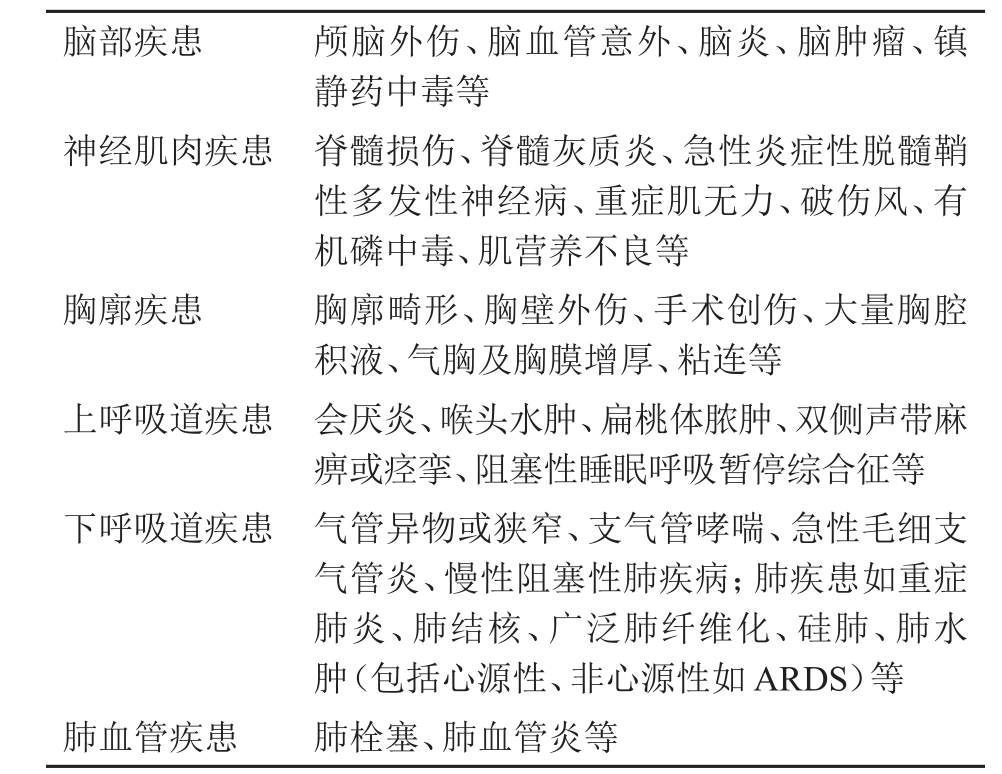
\includegraphics[width=3.33333in,height=2.57292in]{./images/Image00112.jpg}
\end{table}

\hypertarget{text00076.htmlux5cux23CHP3-4-1-1-1}{}
(一) 急性呼吸衰竭与慢性呼吸衰竭

根据起病缓急 ,呼吸衰竭可分为急性和慢性两类,两者之间无明确的时间界限。

\subparagraph{急性呼吸衰竭}

患者既往无呼吸道基础病,因突发因素如溺水、喉头水肿等,在数分钟、数小时甚至数日内发生,病情发展迅速,需及时抢救。

\subparagraph{慢性呼吸衰竭}

多继发于慢性阻塞性肺疾病(COPD)、重症肺结核、间质性肺疾病,起病缓慢,机体产生相应的代偿性改变如血HCO\textsubscript{3}
\textsuperscript{−}
增高。部分患者因合并呼吸道感染、气胸、肺栓塞等情况,病情在短时间内加重,出现PaO\textsubscript{2}
进一步下降和(或)PaCO\textsubscript{2}
显著升高,属于慢性呼吸衰竭急性发作。

\hypertarget{text00076.htmlux5cux23CHP3-4-1-1-2}{}
(二) Ⅰ型呼吸衰竭与Ⅱ型呼吸衰竭

若PaO\textsubscript{2} 低于60mmHg,PaCO\textsubscript{2}
正常或低于正常即为Ⅰ型呼吸衰竭;若PaO\textsubscript{2}
低于60mmHg伴有PaCO\textsubscript{2} 大于50mmHg即为Ⅱ型呼吸衰竭。

\hypertarget{text00076.htmlux5cux23CHP3-4-1-1-3}{}
(三) 泵衰竭与肺衰竭

\subparagraph{泵衰竭}

呼吸中枢、周围神经、呼吸肌和胸廓等驱动或制约呼吸运动的组织器官统称呼吸泵。因呼吸驱动力不足或呼吸运动受限制而引起的呼吸衰竭为泵衰竭,主要表现为通气量不足,出现缺氧伴CO\textsubscript{2}
潴留。

\subparagraph{肺衰竭}

因气道、肺脏、肺血管疾患引起的属肺衰竭。因上呼吸道阻塞引起的呼吸衰竭与泵衰竭相似,主要表现为通气量不足。因肺组织病变引起的呼吸衰竭除通气量下降外,主要为氧合功能障碍,通气/血流比值失调是其主要原因。低氧血症是肺衰竭的共同表现,只有当通气量明显下降时才伴有CO\textsubscript{2}
潴留。

\subsubsection{疾病相关性呼吸衰竭的特点}

临床对于呼吸系统疾病引起的呼吸衰竭较为熟悉,以下主要介绍其他病因所致的呼吸衰竭特点。

\hypertarget{text00076.htmlux5cux23CHP3-4-1-2-1}{}
(一) 脑血管疾病引起的呼吸衰竭

脑疝形成所致呼吸衰竭是脑血管疾病死亡的主要原因之一
。一般认为,病变损害的中枢神经系统部位不同,对呼吸功能的影响也各异。间脑和中脑以上病变可影响呼吸频率,常出现潮式呼吸,即Cheyne-Stokes呼吸;下丘脑视前核病变可诱发急性肺水肿;脑桥受损时,延髓呼吸中枢的调节作用减弱,呼吸变浅而慢;脑桥和中脑的下端损害时,出现过度通气,呈喘息样呼吸;延髓受损主要影响呼吸节律,出现间停呼吸,即Biots呼吸,甚至呼吸暂停。

脑血管疾病导致呼吸衰竭的发生机制与呼吸中枢受到直接损害、颅内压增高、神经源性肺水肿、继发肺部感染等因素有关。

\hypertarget{text00076.htmlux5cux23CHP3-4-1-2-2}{}
(二) 外周神经、肌肉疾患引起的呼吸衰竭

周围神经系统(脑神经核、脊髓、神经根、神经干和神经末梢)病变所致的呼吸衰竭以急性炎症性脱髓鞘性多发性神经病为代表;神经肌肉接头部位病变所致的以重症肌无力危象和有机磷中毒为代表;肌肉本身所致的呼吸衰竭,急性起病者以周期性瘫痪为代表,慢性起病者以多发性肌炎为代表。

急性炎症性脱髓鞘性多发性神经病表现为四肢对称性迟缓性瘫痪,重症患者可出现呼吸衰竭。发生机制主要为呼吸肌麻痹和脑神经受累。以膈肌麻痹为主者表现为腹式呼吸减弱或消失,可出现腹式矛盾呼吸;以肋间肌麻痹为主者可表现为胸式矛盾呼吸。脑神经受累者可出现吞咽困难、呛咳、咳痰无力,分泌物在气道蓄积,诱发呼吸衰竭。

\hypertarget{text00076.htmlux5cux23CHP3-4-1-2-3}{}
(三) 外科手术引起的呼吸衰竭

外科患者约 25\%的术后死因与肺部并发症相关
。因此,麻醉和外科手术对患者呼吸功能的影响不容忽视。

\subparagraph{麻醉对呼吸功能的影响}

全身麻醉对呼吸中枢、呼吸肌和肺脏均有影响。吸入常规剂量的麻醉剂在抑制呼吸的同时,也抑制甚至阻断机体对低氧血症和高碳酸血症的反应。全身麻醉可引起膈肌和肋间肌张力立即丧失,出现膈肌上抬、胸腔容积缩小,导致功能残气容积减少,并可引起肺不张。肺不张不仅降低肺泡通气,更使肺内分流增加。对于有肺脏基础疾病如COPD、间质性肺炎患者,麻醉剂的上述效应可能诱发术后低氧血症、甚至呼吸衰竭。

\subparagraph{手术对呼吸功能的影响}

胸部和上腹部手术对呼吸功能的影响最大,可表现为肺活量和功能残气容积显著减少。肺切除术对呼吸功能的影响不言而喻。开胸手术对胸壁造成的创伤,使胸壁顺应性明显下降。心脏手术如冠状动脉旁路移植术可造成肺组织挫伤、左侧膈神经损伤和肺不张等,严重影响肺的氧合功能。体外循环因缺血再灌注等因素可导致肺泡毛细血管膜损伤,出现急性肺损伤。上腹部手术因引起膈肌功能不全而显著影响呼吸功能,如上腹部手术后24小时内,潮气量可降低50\%,而下腹部手术后仅下降约25\%。

\subparagraph{外科手术后发生呼吸衰竭的常见原因}

①肺不张:是胸部和上腹部手术后的常见并发症。除手术因素外,麻醉剂的滞留效应、术后疼痛、体质虚弱等使患者不能有效咳嗽,造成呼吸道分泌物阻塞气道,出现肺不张。②肺炎:属院内感染。胸部和上腹部手术是医院获得性肺炎的独立危险因素。术前存在基础疾病如COPD、低白蛋白血症、长期吸烟、高龄、昏迷、术后留置鼻胃管、接受机械通气治疗等均为医院获得性肺炎的危险因素。③误吸:系指口咽部和胃内容物吸入喉及下呼吸道的过程。误吸占麻醉相关的死因约10\%~30\%。麻醉所致的意识障碍、气管插管对咽喉部的刺激、药物及腹部手术对胃肠动力学影响,容易引起患者恶心、呕吐,加之声门闭合功能不全,导致胃内容物误吸,形成化学性肺炎,严重者出现ARDS。肺损伤的程度与吸入发生的频率、吸入物的pH和容量以及机体对吸入物的反应等有关。pH
< 2.5和胃酸吸入量>
0.3ml/kg被认为是导致肺脏发生炎症的阈值。误吸胃酸早期以化学性炎症为主,随后多继发细菌性感染。对于存在吞咽困难的老年患者,常误吸含有定殖细菌的口咽部分泌物,此时肺部早期也会出现细菌性炎症。

\hypertarget{text00076.htmlux5cux23CHP3-4-1-2-4}{}
(四) 药源性呼吸衰竭

药物可通过以下 4个方面影响呼吸功能
:①中枢性肺泡低通气:除麻醉药外,几乎所有的镇静剂能抑制呼吸中枢。临床常用的硝西泮和氟西泮容易引起呼吸抑制,COPD伴轻度高碳酸血症的患者因精神兴奋而失眠,服用常规剂量的该类药物后常表现缺氧和高碳酸血症的进一步加重,出现昏迷甚至死亡。应用重复剂量或大剂量的苯唑西泮对呼吸的抑制作用长于镇静作用,部分患者在没有意识障碍的情况下出现中枢性呼吸衰竭。过量的抗精神病药和H\textsubscript{1}
受体拮抗剂也可引起中枢性肺泡低通气。此外,西咪替丁、可乐定和利多卡因等也可引起呼吸暂停。②神经肌肉阻滞:氨基糖苷类、多黏菌素、新霉素、钙通道阻滞剂等通过影响运动神经冲动传导抑制呼吸肌功能,重症肌无力患者对上述药物特别敏感。③药物引起肌肉病变:长期大剂量使用糖皮质激素、氟烷、乙醚等药物可引起肌肉病变,表现为急性疼痛性肌病、慢性无痛性肌病,甚至肌强直,呼吸肌运动受限,严重者发生呼吸衰竭。④药物性肺水肿:海洛因、水杨酸盐、苯妥英钠、双氢克尿塞、右旋糖酐、美沙酮、氨甲蝶呤、麻醉药过量等可引起肺微血管通透性增加导致非心源性肺水肿。

\subsubsection{呼吸衰竭发病机制}

缺氧和CO\textsubscript{2} 潴留是呼吸衰竭的基本病理生理变化。

\hypertarget{text00076.htmlux5cux23CHP3-4-1-3-1}{}
(一) 缺氧的发生机制

\subparagraph{通气障碍}

健康成人呼吸空气时总肺泡通气量达到4L/min才能保证有效的气体交换,维持正常的肺泡O\textsubscript{2}
分压和CO\textsubscript{2}
分压。肺泡通气量严重不足既导致缺氧,又造成CO\textsubscript{2}
潴留。呼吸运动有赖于呼吸中枢驱动、神经传导、吸气肌收缩、横膈下降、胸廓和肺泡的扩张。上述任何一个环节的障碍如呼吸中枢抑制、呼吸肌疲劳、胸廓和肺顺应性降低等均可导致肺扩张受限,出现限制性肺泡通气不足。阻塞性肺泡通气不足主要因气道阻力增加而引起,COPD、支气管哮喘等是其常见原因。

\subparagraph{换气障碍}

①通气/血流比值失调:肺有效气体交换不仅要求有足够的通气量与血流量,而且要求两者的比例适当。健康成人呼吸空气时的肺血流量约为5L/min,故全肺通气/血流比值大约为0.8。比值小于0.8见于部分肺泡通气不足,如肺水肿、肺炎、肺不张等;比值大于0.8见于部分肺泡血流不足,如肺栓塞、肺毛细血管床广泛破坏、部分肺血管收缩等。②弥散障碍:见于呼吸膜增厚(如肺水肿)和面积减少(如肺不张、肺实变),或肺毛细血管血量不足(肺气肿)及血液氧合速率减慢(贫血)等。因O\textsubscript{2}
的弥散能力仅为CO\textsubscript{2}
的1/20,故存在弥散障碍时,通常以缺氧为主。单纯换气障碍所致的血气变化特点:PaO\textsubscript{2}
下降,PaCO\textsubscript{2}
正常或降低;肺泡-动脉血氧分压差P(A-a)O\textsubscript{2} 增大。

\subparagraph{肺内动-静脉解剖分流增加}

肺动脉内的静脉血未经氧合直接流入肺静脉,导致PaO\textsubscript{2}
下降,常见于肺动-静脉瘘。

\subparagraph{氧耗量增加}

发热、呼吸困难、应激等均可增加氧耗量,是加重缺氧的常见原因。

\hypertarget{text00076.htmlux5cux23CHP3-4-1-3-2}{}
(二) CO\textsubscript{2} 潴留的发生机制

PaCO\textsubscript{2} 水平取决于CO\textsubscript{2}
的生成量与排出量。CO\textsubscript{2}
生成量增加见于发热、甲状腺功能亢进症等,极少引起PaCO\textsubscript{2}
升高。CO\textsubscript{2}
潴留主要因肺泡通气不足引起。因此,PaCO\textsubscript{2}
是反映肺泡通气量的最佳指标,其升高表明肺泡通气不足。

\subsubsection{呼吸衰竭对机体的影响}

呼吸衰竭时发生的缺氧和CO\textsubscript{2}
潴留,可影响全身各系统的代谢和功能。它们对机体的危害程度既与PaO\textsubscript{2}
和PaCO\textsubscript{2} 的绝对值有关,更与PaO\textsubscript{2}
下降或PaCO\textsubscript{2} 上升的速度和持续时间有关。

\hypertarget{text00076.htmlux5cux23CHP3-4-1-4-1}{}
(一) 中枢神经系统变化

中枢神经系统对缺氧十分敏感
。缺氧程度不同,其影响也各异。PaO\textsubscript{2}
降至60mmHg时,可出现注意力不集中、智力和视力轻度减退;PaO\textsubscript{2}
低于50mmHg时,患者烦躁不安、定向与记忆障碍、谵妄;PaO\textsubscript{2}
低于30mmHg时,患者意识丧失,陷入昏迷;PaO\textsubscript{2}
低于20mmHg时,几分钟内神经细胞可发生不可逆性损害。缺氧发生的缓急及个体差异性也影响上述变化的出现。

CO\textsubscript{2} 参与脑血流调节。当PaCO\textsubscript{2}
在100mmHg内,PaCO\textsubscript{2}
每增加10mmHg,脑血流量增加50\%。PaCO\textsubscript{2}
大于80mmHg时,患者头痛、烦躁不安、扑翼样震颤;PaCO\textsubscript{2}
大于90mmHg时,可出现昏迷,即所谓“CO\textsubscript{2}
麻醉”。PaCO\textsubscript{2}
增高引起的昏迷与其发生速度有关。慢性呼吸衰竭患者耐受性较高,PaCO\textsubscript{2}
达到100mmHg,仍可保持神志清醒。

呼吸衰竭引起的神经精神状态综合征称为肺性脑病(pulmonary
encephalopathy),早期表现为头痛、头昏、失眠、兴奋、烦躁不安和睡眠倒错,晚期还可出现昏迷、谵妄、精神错乱、抽搐和呼吸抑制。肺性脑病的发病机制为缺氧、CO\textsubscript{2}
潴留和酸中毒三个因素共同作用损伤脑血管和脑细胞。正常脑脊液的缓冲作用较血液弱,其pH也较低。血液中HCO\textsubscript{3}
\textsuperscript{−} 和H\textsuperscript{+}
不易通过血脑屏障进入脑脊液,因此,脑脊液的酸碱调节需时较长。CO\textsubscript{2}
潴留时,脑脊液pH降低明显。当脑脊液pH低于7.25时,脑电波变慢,pH低于6.8时,脑电活动完全停止。缺氧和CO\textsubscript{2}
潴留均会使脑血管扩张。缺氧损伤血管内皮细胞,使其通透性增高,导致脑间质水肿。缺氧导致细胞ATP生成减少造成细胞膜Na\textsuperscript{+}
-K\textsuperscript{+}
泵功能障碍,引起细胞内高钠和水增多,形成脑细胞水肿。此外,脑细胞内的酸中毒可引起抑制性神经递质γ-氨基丁酸生成增多,加重中枢神经系统的功能和代谢障碍。

\hypertarget{text00076.htmlux5cux23CHP3-4-1-4-2}{}
(二) 循环系统变化

缺氧和 CO\textsubscript{2}
潴留均可兴奋心血管运动中枢,使心肌收缩力增强、心率增快、心排出量增加。它们对机体不同部位血管的作用各异,脑血管和冠状动脉扩张,肺、肾及其他腹腔脏器血管收缩。缺氧可致皮肤血管轻度收缩,而CO\textsubscript{2}
潴留则使之扩张。长期缺氧和CO\textsubscript{2}
潴留可引起肺小动脉收缩、形成慢性肺动脉高压,导致右心室肥大。

\hypertarget{text00076.htmlux5cux23CHP3-4-1-4-3}{}
(三) 呼吸系统变化

PaO\textsubscript{2}
降低刺激外周化学感受器,反射性增强呼吸运动,此反应在PaO\textsubscript{2}
降至60mmHg时才明显,为一种保护性反射调节。当PaO\textsubscript{2}
降至30mmHg时,严重缺氧直接抑制呼吸中枢。PaCO\textsubscript{2}
升高主要刺激中枢化学感受器,引起呼吸加深加快;长时间严重CO\textsubscript{2}
潴留会造成中枢化学感受器对CO\textsubscript{2}
的刺激效应发生适应;当PaCO\textsubscript{2}
升至80mmHg时,反而抑制呼吸中枢,此时,呼吸运动主要靠缺氧对外周化学感受器的刺激而得以维持。

\hypertarget{text00076.htmlux5cux23CHP3-4-1-4-4}{}
(四) 其他系统变化

缺氧可引起肝细胞水肿、变性、甚至坏死,使丙氨酸氨基转移酶上升;严重缺氧因使胃壁血管收缩而降低胃肠黏膜的屏障作用、CO\textsubscript{2}
潴留则可引起胃酸分泌增多,其共同作用的结果是导致消化不良、食欲不振,甚至胃肠黏膜糜烂、溃疡及出血;缺氧和CO\textsubscript{2}
潴留均可引起肾血管收缩,致肾血流量减少,轻者尿中出现蛋白、红细胞、白细胞,严重者发生急性肾功能衰竭。慢性缺氧产生继发性红细胞增多,血液黏稠度增加等。当缺氧得到纠正时,受损的肝、肾功能可逐渐恢复正常。

\subsection{诊断}

\subsubsection{临床表现特点}

呼吸衰竭的临床表现因原发病的不同而有很大差异,但均以缺氧和(或)CO\textsubscript{2}
潴留对机体的影响为基本表现,出现一些典型的症状和体征。

\subparagraph{呼吸困难}

是呼吸衰竭最早出现的重要症状。患者主观感为气急,客观表现为呼吸用力,伴有呼吸频率、深度与节律的改变。出现点头或提肩呼吸,有时还可见鼻翼扇动、端坐呼吸。上呼吸道疾患常表现为吸气性呼吸困难,可有三凹征。呼气性呼吸困难多见于下呼吸道不完全阻塞如支气管哮喘等。胸廓疾患、重症肺炎等表现为混合性呼吸困难。呼吸肌疲劳时会出现呼吸浅快、腹式反常呼吸,如吸气时,腹壁内陷。呼吸衰竭并不一定有呼吸困难,如镇静药中毒患者可表现呼吸匀缓、表情淡漠或昏睡。

\subparagraph{发绀}

是缺氧的典型体征,舌色发绀较口唇、甲床更明显。因发绀是由血液中还原血红蛋白的绝对值增多引起,故重度贫血患者即使有缺氧也并不一定有发绀。

\subparagraph{神经精神症状}

急性呼吸衰竭的神经精神症状较慢性明显。急性严重缺氧可出现谵妄、抽搐、昏迷。慢性者则可有注意力不集中、智力或定向功能障碍。CO\textsubscript{2}
潴留出现头痛、肌肉不自主抽动或扑翼样震颤,以及中枢抑制之前的兴奋症状如失眠、睡眠倒错、烦躁等,后者常是呼吸衰竭的早期表现。

\subparagraph{循环系统症状}

缺氧和CO\textsubscript{2}
潴留均可导致心率增快、血压升高。严重缺氧可出现各种类型的心律失常,甚至心脏停搏。CO\textsubscript{2}
潴留可引起多汗、球结膜充血和水肿、颈静脉充盈等。长期缺氧则引起肺动脉高压、右心室肥大,出现相应体征。

\subparagraph{其他脏器的功能障碍}

严重缺氧和CO\textsubscript{2}
潴留可导致肝肾功能障碍,出现黄疸、肝功能异常、上消化道出血;血尿素氮、肌酐增高,尿中出现蛋白、管型等。

\subparagraph{酸碱失衡和水、电解质紊乱}

因缺氧而过度通气可发生呼吸性碱中毒。CO\textsubscript{2}
潴留则表现为呼吸性酸中毒。长时间严重缺氧则出现代谢性酸中毒及电解质紊乱。

\subsubsection{血气分析与诊断注意事项}

呼吸衰竭的诊断主要依靠动脉血气分析。目前仍采用PaO\textsubscript{2} <
60mmHg和(或)PaCO\textsubscript{2} >
50mmHg作为诊断指标。临床应用时,应注意以下几点:

1.一般情况下 ,只要呼吸平稳,PaCO\textsubscript{2}
比较稳定,而PaO\textsubscript{2}
则随年龄、海拔、氧疗和体位等变化而有较大差异。阻塞性睡眠呼吸暂停综合征患者PaO\textsubscript{2}
和PaCO\textsubscript{2}
存在昼夜节律性变化,白天基本正常,夜间出现明显低氧血症和高碳酸血症,达到呼吸衰竭诊断标准。

2.对于无血气分析的基层医疗单位 ,可根据SaO\textsubscript{2}
与PaO\textsubscript{2} 的对应关系,大致推算出PaO\textsubscript{2}
。SaO\textsubscript{2} 为90\%时,PaO\textsubscript{2}
对应于60mmHg;SaO\textsubscript{2}
在85\%~90\%之间,PaO\textsubscript{2}
为50~60mmHg;SaO\textsubscript{2} 在75\%~85\%时,PaO\textsubscript{2}
为40~50mmHg。

3.低氧血症是氧合功能障碍的共同表现,只有当肺泡通气量明显下降时才伴有CO\textsubscript{2}
潴留。故PaO\textsubscript{2} 降低患者的PaCO\textsubscript{2}
可降低、正常或升高;但PaCO\textsubscript{2}
升高者常有PaO\textsubscript{2}
降低;仅在氧疗过程中出现PaCO\textsubscript{2} 升高伴PaO\textsubscript{2}
正常。而且,COPD以外的疾患如出现CO\textsubscript{2}
潴留,多提示病情危重。

4.慢性高碳酸血症因肾脏的代偿
,pH常趋于正常。通常可根据pH判定PaCO\textsubscript{2}
是否为急性增加,急性呼吸衰竭时,PaCO\textsubscript{2}
每升高10mmHg,pH下降0.08;慢性呼吸衰竭时,PaCO\textsubscript{2}
每升高10mmHg,pH下降0.03。如无代谢性酸中毒,任何水平的高碳酸血症伴有pH
< 7.30,均应考虑急性呼吸衰竭。

5.ARDS虽属急性呼吸衰竭,但因其发病机制、病理及临床表现具有特殊性,故有其相应的诊断标准,详见本书第29章“急性肺损伤与急性呼吸窘迫综合征”。

\subsection{治疗}

\subsubsection{急性呼吸衰竭的治疗}

治疗原则首先是保持呼吸道通畅、吸氧并维持适宜的肺泡通气,其次为明确病因、治疗原发病及对症支持治疗。

\hypertarget{text00076.htmlux5cux23CHP3-4-3-1-1}{}
(一) 保持呼吸道通畅

通畅的呼吸道是实施各种呼吸急救措施的必要条件
。呼吸骤停患者常因体位不当、舌后坠、口咽部肌肉松弛、呼吸道分泌物等导致上呼吸道阻塞。呼吸急救的要点是使患者取仰卧位,头后仰、下颌向前,迅速清除呼吸道分泌物或异物。口对口呼吸是一种简便而有效的临时急救措施。若患者牙关紧闭,则可改为口对鼻呼吸。当上气道阻塞不能解除时,可行紧急环甲膜切开术开放气道。

若经上述处理,仍难以维持呼吸道通畅,或因病情需要长时间维持肺泡通气者,则需及时建立人工气道。一般有简便人工气道、气管插管、气管切开三种方法。简便人工气道主要有口咽通气道、鼻咽通气道和喉罩。气管插管和气管切开是重建呼吸道最为可靠的方法。紧急情况下多选择经口插管,其操作速度快于经鼻插管。经鼻插管容易被清醒患者耐受,但鼻窦炎发生率较高。

目前使用的气管插管或气管切开管的气囊多为低压高容型,对气管黏膜的损伤较小,不再提倡定期气囊放气。一般认为,气囊的压力维持在25cmH\textsubscript{2}
O以下较为安全。建立人工气道后,应注意在无菌条件下行气道内分泌物的吸引和气道的湿化。

\hypertarget{text00076.htmlux5cux23CHP3-4-3-1-2}{}
(二) 氧疗

通过增加吸入氧浓度纠正患者缺氧状态的方法即为氧疗。对于急性呼吸衰竭患者,氧疗是改善缺氧的重要手段。氧疗后尽可能使动脉血氧饱和度>
90\%。

\subparagraph{鼻导管或鼻塞给氧}

为常用吸氧工具,简单、方便,不影响患者咳痰、进食。缺点为氧浓度不稳定,随患者呼吸深度和频率的变化而异,并且刺激局部黏膜。鼻导管经鼻孔缓慢插入,直达软腭水平(离鼻孔8~10cm)。鼻塞一端与输氧管连接,另端塞入鼻前庭约1cm即可,该法较鼻导管舒服。吸入氧浓度(FiO\textsubscript{2}
)的计算可参照经验公式:FiO\textsubscript{2} (\%)= 21 + 4
×氧流量(L/min)。

\subparagraph{面罩给氧}

适用于PaO\textsubscript{2}
明显降低,对氧流量需求较大的患者。包括简单面罩、带储气囊无重复呼吸面罩等,优点为吸入氧浓度相对稳定,对鼻黏膜刺激小,但有时影响患者的进食和咳痰。

\subparagraph{高压氧治疗}

系指在超过1个大气压(atm)的高压情况下给氧,利用氧分压与血液氧溶解度呈正比的关系以增加血氧含量,最终达到缓解组织缺氧的目的。通常需将患者送入高压氧舱内,在1.2~3.0atm下吸氧。高压氧治疗主要适用于外呼吸功能正常,而氧在血液的运输发生障碍所导致的Ⅰ型呼吸衰竭,如一氧化碳或氰化物中毒、减压病等。

需指出:①氧疗仅仅是对症治疗,缺氧的最终改善取决于原发病处理;②氧疗对不同原因所致缺氧的效果有所差异,单纯因通气不足引起者对氧疗较敏感;其次为轻、中度通气血流/比值失调和弥散障碍所致缺氧;效果最差的为重度肺换气功能障碍如肺内分流所致缺氧;③通常PaO\textsubscript{2}
升至50~60mmHg,SaO\textsubscript{2}
在85\%~90\%以上时能够基本满足机体的氧代谢需要;④氧疗的最终目的是通过提高PaO\textsubscript{2}
改善组织缺氧,若循环功能不全,即使PaO\textsubscript{2}
正常,因氧运输障碍也可能出现组织缺氧。此外,氧的运输主要以氧与血红蛋白结合的方式进行,严重贫血患者也出现氧运输障碍,故一般要求血红蛋白的水平不低于100~120g/L。

氧疗过程中,还应避免下列并发症的发生:①氧中毒:长时间高浓度吸氧可致呼吸系统、中枢神经系统和视网膜的毒性作用。氧中毒也是ARDS的诱因之一。紧急情况下,FiO\textsubscript{2}
越高,纠正缺氧的效果越好,一旦病情缓解,即应及时控制FiO\textsubscript{2}
。在常压下,FiO\textsubscript{2}
为25\%~40\%较为安全。由于氧解离曲线的S形特点,PaO\textsubscript{2} >
80mmHg后不会再显著增加血氧含量,故应选择能保持合适PaO\textsubscript{2}
的最低FiO\textsubscript{2} 。②CO\textsubscript{2}
潴留:氧疗后CO\textsubscript{2}
潴留加重,常见于COPD并发Ⅱ型呼吸衰竭。部分原因为原先存在的缺氧性通气驱动受到抑制。③吸收性肺不张:呼吸空气时,肺内含有大量不被吸收的氮气。高浓度氧疗时,肺泡气中氮逐渐为氧所取代,氧易被血液吸收而发生肺泡萎陷。存在气道阻塞时,易发生吸收性肺不张。

\hypertarget{text00076.htmlux5cux23CHP3-4-3-1-3}{}
(三) 机械通气

机械通气不仅用于治疗不同病因所致的呼吸衰竭
,而且也用于预防呼吸衰竭的发生或加重。对心胸大手术后和严重胸部创伤患者,利用呼吸机帮助患者渡过呼吸负荷加重阶段。关于机械通气模式的选择、参数的调整可参照本书第136章“人工呼吸机的临床应用”。

对于大多数接受气管插管、机械通气的患者,均主张给予低水平的PEEP(3~5cmH\textsubscript{2}
O),以补偿因仰卧体位和经喉插管引起的容量下降。对于氧合不满意的患者,可提高PEEP水平。调节PEEP的水平应在最合适的吸入氧浓度(小于0.6)条件下达到较好地动脉血氧合,通常不超过15cmH\textsubscript{2}
O。有条件者根据P-V曲线选择,PEEP应高于低拐点2cmH\textsubscript{2} O。

\hypertarget{text00076.htmlux5cux23CHP3-4-3-1-4}{}
(四) 体外膜肺氧合

体外膜肺氧合(extracorporeal membrane
oxygenation,ECMO)为体外心肺功能辅助装置,利用体外循环代替自然循环,通过引流患者的静脉血,经人工肺氧合并排出二氧化碳,再用泵将血液经静脉或动脉输回患者体内。主要有静脉-动脉(V-A法)和静脉-静脉(V-V法)ECMO两种方式,它可以使肺得到休息,为患者提供有效呼吸支持,使患者渡过呼吸机支持无效的危重时期,为原发病的治疗争取时间。目前主要用于重度急性呼吸衰竭经机械通气治疗效果不佳的患者如新生儿呼吸窘迫综合征、ARDS、先天性膈疝等。现有的资料表明,ECMO治疗新生儿及儿童呼吸衰竭的存活率高于成人。

推荐EMCO的纳入标准为:①在吸入纯氧条件下,PaO\textsubscript{2}
/FiO\textsubscript{2} < 100,或肺泡动脉氧压差>
600mmHg,或失代偿高碳酸血症pH < 7.20;②年龄< 65岁;③接受机械通气时间<
7天;④无抗凝禁忌证;⑤非濒死患者。

ECMO并发症主要有出血、血栓、感染、肢体缺血性损伤、肾功能不全等,其中出血是严重的并发症,需定期检测凝血酶原时间,依此调节肝素用量;机械方面并发症有回路血栓堵塞或脱落、氧合器功能不良、机械故障、置管和拔管相关并发症等。

\hypertarget{text00076.htmlux5cux23CHP3-4-3-1-5}{}
(五) 一般支持治疗

1.控制感染
呼吸道感染既可诱发或加重呼吸衰竭,同时也是呼吸衰竭和机械通气的常见并发症。应在气道分泌物引流通畅的条件下,选用适宜的抗菌药控制感染。

2.纠正酸碱失衡
急性呼吸衰竭较慢性呼吸衰竭更易合并代谢性酸中毒,应积极纠正。

3.注意心血管、脑、肾功能的维持以及水、电解质平衡。

\hypertarget{text00076.htmlux5cux23CHP3-4-3-1-6}{}
(六) 病因治疗

是呼吸衰竭治疗的根本。急性呼吸衰竭多有突发的病因,通常根据病史、体检、胸片及动脉血气作出判断。针对不同病因,采取相应的措施是治疗急性呼吸衰竭的根本所在。上述各种治疗的目的也在于为原发病的治疗争取时间和创造条件。

\subsubsection{慢性呼吸衰竭的治疗}

治疗原则是改善和纠正缺氧、CO\textsubscript{2}
潴留以及代谢功能紊乱,提高生活质量;预防或减轻并发症的发生及程度;积极治疗基础疾病中的可逆性病变成分。

\hypertarget{text00076.htmlux5cux23CHP3-4-3-2-1}{}
(一) 保持呼吸道通畅

原则与急性呼吸衰竭基本一致。

\subparagraph{支气管扩张剂}

对于COPD或存在有气道高反应性的患者,应使用支气管扩张剂。常用茶碱、β\textsubscript{2}
受体激动剂和抗胆碱能药,对于后两类药首选吸入制剂。使用茶碱和β\textsubscript{2}
受体激动剂过程中,需注意心脏的不良反应。目前已将吸入抗胆碱能药作为COPD患者的一线治疗药物,常用溴化异丙托品和噻托溴铵。前药为短效制剂,吸入后5~10分钟起效,持续4~6小时;后者为长效剂,每天一次吸入治疗,可保持24小时疗效。

\subparagraph{祛痰剂}

呼吸道分泌物过多或不易排出常加重通气障碍,使病情进一步恶化。可用溴己新或氨溴索祛痰,后者的作用较前者强,它不仅降低痰液黏度,而且增强黏膜纤毛运动,促进痰液排出。另可选用中药鲜竹沥液等。

\subparagraph{湿化及雾化治疗}

湿化吸入气体和雾化给药均可达到净化、湿化气道及局部治疗(解痉、消炎、祛痰等)作用。理想的雾化要求:等渗液体、雾滴直径为1~3μm、雾化气体的水分应达到100mg/L、深而慢的口呼吸,并在吸气后适当屏气。湿化和雾化治疗的局部用药有β\textsubscript{2}
受体激动剂、抗胆碱能药物、抗生素、激素等。治疗中应避免交叉感染、气道痉挛及干稠分泌物湿化后的膨胀作用。

\subparagraph{胸部理疗}

凡气道分泌物增多、黏稠或分泌物的自然清除机制受损时,可考虑胸部理疗,如体位引流、拍击、振荡和深呼吸等。

\hypertarget{text00076.htmlux5cux23CHP3-4-3-2-2}{}
(二) 氧疗

长期家庭氧疗对
COPD并发慢性呼吸衰竭患者具有重要作用,已证明它可降低患者肺动脉高压、明显改善生活质量、提高存活率。要求吸氧持续时间不应少于15h/d。

严重缺氧患者可在短时间内吸入高浓度氧,随后应及时将吸氧浓度调节至纠正缺氧的最低水平。对于Ⅱ型呼吸衰竭患者强调控制性氧疗,因为吸氧可能会加重CO\textsubscript{2}
潴留和呼吸性酸中毒。

\hypertarget{text00076.htmlux5cux23CHP3-4-3-2-3}{}
(三) 机械通气治疗

\subparagraph{无创通气}

循证医学支持COPD急性加重期、心源性肺水肿、免疫功能低下并呼吸衰竭及辅助拔管的COPD患者行无创通气。无创性通气可减轻呼吸肌疲劳,也适用于家庭治疗。无创通气对饮食、谈话影响小,减少了气管插管或气管切开的并发症如呼吸机相关肺炎的发生率,可缩短住院时间。

接受无创通气的患者需具备下列条件:①意识清醒,具备咳痰和自主呼吸能力;②血流动力学稳定;③无面部和上呼吸道外伤;④无严重心律失常、无未经引流的气胸或纵隔气肿和严重腹胀、无误吸、无气道分泌物过多且排痰不利等情况;⑤有良好的配合能力等。

临床常用双水平气道正压通气(BiPAP)辅助通气。BiPAP可以对吸气相和呼气相气道压分别进行调节,在吸气时提供较高的压力(10~25cmH\textsubscript{2}
O),在呼气时提供较低的压力(3~5cmH\textsubscript{2}
O)。BiPAP的主要缺点是不能保证有效通气量。无创通气失败的常见原因有:患者不合作或不能耐受面罩或有恐怖感;鼻(面)罩不合适,漏气大;气道内存在大量分泌物或不能有效咳嗽。

应用无创通气过程中需要及时、准确地判断疗效,以确定是继续应用还是转换为有创通气。一般认为,应用无创通气1~2小时后,如果病情恶化或患者不耐受,应及时转为有创通气。

\subparagraph{有创通气}

目前尚无明确、统一的标准来决定呼吸衰竭患者是否接受有创通气治疗。对不同原因所致的呼吸衰竭,上机的标准应有所差异。机械通气仅仅是一种支持呼吸功能的手段,对原发病并无治疗作用,其价值在于为诊治原发病及呼吸功能的恢复争取时间。上机之前应充分估计原发病是否可逆、有无撤机的可能,并综合考虑医疗、社会、经济等诸多因素。

临床可根据患者的一般情况(意识、呼吸频率及节律、自主排痰能力)及动脉血气指标的动态变化判定。当出现意识障碍、呼吸频率过快或过慢(如>
35~40次/分或< 8
次/分);呼吸节律不规则;无力咳痰;或自主呼吸微弱或消失;吸氧条件下PaO\textsubscript{2}
< 50mmHg;PaCO\textsubscript{2}
进行性升高,pH动态下降。提示需及时使用有创通气。对COPD急性加重所致的慢性呼吸衰竭,选择上机的PaO\textsubscript{2}
值一般较急性呼吸衰竭低。

根据患者的呼吸情况,选择控制性或辅助性通气模式。前者适用于自主呼吸不规则、减弱或消失,后者适用于自主呼吸存在并与呼吸机协调良好的患者。目前尚无充分的依据证明哪种模式最好,总的原则是当病情趋于稳定时尽早由控制模式改为辅助模式。有气道阻塞或存在肺部疾患时,宜选用同步性能好的呼吸机,以减少人机对抗并确保肺泡通气量的稳定。脑部及神经肌肉疾患所致的呼吸衰竭,因肺功能正常,各种类型的呼吸机均可选用。

为克服传统机械通气的局限性,目前提倡一些新的机械通气策略,循证医学将小潮气量(6ml/kg理想体重)通气作为肺保护策略的A级推荐意见,因其能有效避免机械通气相关的肺损伤。同时注意平台压应小于35cmH\textsubscript{2}
O。肺开放策略是指采用肺复张手法,即一次或多次给予高于常规平均气道压的压力并维持一定的时间(一般不超过2分钟)。肺复张手法一方面能使更多的萎陷肺泡开放,另一方面还可以防止小潮气量通气所带来的继发性肺不张,从而能达到减少肺损伤和改善肺顺应性及氧合目的。

\subparagraph{有创 -无创序贯通气的应用}

患者接受有创通气后,当呼吸衰竭得到一定程度缓解但尚未达到传统的拔管-撤机标准之前,代之以无创通气,从而减少有创通气的时间,称之为有创-无创序贯通气策略。多项研究证实该法可显著提高撤机成功率,缩短机械通气和住ICU的时间,降低院内感染率,增加患者存活率。

有创-无创序贯通气能否成功的关键是把握有创通气转为无创通气的切换点,王辰等提出对于COPD急性加重期患者以肺部感染控制窗作为切换点,能较准确地判断早期拔管时机。通过使用有效抗菌药和及时引流人工气道内痰液后,支气管-肺部感染往往在5~7天内得到控制,表现为痰量减少、黏度变稀、痰色转白、体温下降、血白细胞计数降低、X线胸片上支气管-肺部感染影消退,此阶段称为肺部感染控制窗。肺部感染控制窗后若不及时拔管,则可能随插管时间延长并发呼吸机相关肺炎。出现肺部感染控制窗时患者痰液引流问题已不突出,而呼吸肌疲劳仍较明显,需要较高水平的通气支持,此时撤离有创通气,继之无创通气,能进一步缓解呼吸机疲劳,改善通气功能,明显减少再插管或气管切开。

\subparagraph{疾病特异性的机械通气治疗}

\hypertarget{text00076.htmlux5cux23CHP3-4-3-2-3-4-1}{}
(1) COPD:

COPD患者因病情反复发作,需多次接受机械通气治疗,原则上选择气管插管,尽量避免气管切开。一般可采用辅助通气模式,以PSV较常用,压力支持从低压(10cmH\textsubscript{2}
O)开始,逐渐增加压力,最高压力以≤30cmH\textsubscript{2}
O为妥。由于PSV的主要缺点是没有通气量的保证,临床可采用SIMV +
PSV,必要时设置MMV功能以保障通气安全。

COPD急性发作期患者几乎均存在内源性呼气末正压(PEEPi),故可在呼气末加用一定的正压(通常为3~5cmH\textsubscript{2}
O),以减少呼吸肌克服PEEPi作功,促进人机协调。患者多有慢性呼吸性酸中毒,因肾脏的代偿,体内{}
增加,若CO\textsubscript{2}
排出过快,容易从酸中毒转变为碱中毒。故原则上使PaCO\textsubscript{2}
逐渐下降,在1~2天达到或稍低于患者急性发作前的水平即可。

\hypertarget{text00076.htmlux5cux23CHP3-4-3-2-3-4-2}{}
(2) 神经肌肉性疾病:

主要为泵衰竭,由呼吸肌无力所致,患者的中枢呼吸驱动及肺换气功能基本正常。因呼吸肌无力使肺不能充分膨胀,易发生肺不张,可采用较大的潮气量(12ml/kg),必要时加用呼气末正压(5~10cmH\textsubscript{2}
O)或叹息(sigh)功能,以防止肺不张。该类患者肺功能基本正常,只要保证足够的通气量,吸入较低浓度的氧(FiO\textsubscript{2}
为0.25~0.35),即可维持动脉血气于正常水平。对病情进展缓慢、延髓呼吸中枢功能正常、气道分泌物不多的患者可选择无创通气。一般根据患者自主呼吸力量的强弱,选择控制或辅助性通气模式。估计短期内有可能脱离机械通气者,可选用气管插管建立人工气道,若机械通气超过2周以上者,则应行气管切开。

\hypertarget{text00076.htmlux5cux23CHP3-4-3-2-3-4-3}{}
(3) 脑部病变:

常见由脑血管意外、颅脑外伤、脑炎等所致的中枢性呼吸衰竭。原则与神经肌肉性疾病的机械通气治疗类似。当伴有颅内高压时,可采用控制性过度通气,使PaCO\textsubscript{2}
保持在25~30mmHg范围内,脑血管处于轻度收缩状态,以利于降低颅内压。颅内高压改善后,应逐渐减低通气量,使PaCO\textsubscript{2}
恢复正常。部分患者的咳嗽反射减弱甚至消失,容易并发下呼吸道感染,应注意人工气道的护理。

\hypertarget{text00076.htmlux5cux23CHP3-4-3-2-3-4-4}{}
(4) 外科手术后:

外科术后呼吸功能减退的发生率较高,常见于胸腹部手术后。因术后肺不张、间质性肺水肿、误吸、肺部感染等引起。心胸外科手术、原有肺部基础疾患接受上腹部手术后,呼吸衰竭发生率较高,对此类患者可积极行机械通气治疗,帮助患者顺利渡过术后数日内呼吸功能明显下降这一关键阶段。因胸腹部手术切口对呼吸运动有一定影响,可设置相对较小潮气量及较快通气频率。可选用PSV或CPAP等通气模式。

\hypertarget{text00076.htmlux5cux23CHP3-4-3-2-4}{}
(四) 抗感染治疗

因住院时间久
、免疫功能低下或缺陷、接受机械通气治疗等因素,患者易发生医院获得性下呼吸道感染。因此,选择有效的抗菌药物、采用适当的剂量和疗程控制感染十分重要。临床可通过呼吸系统症状和体征的变化、体温、外周血象、C反应蛋白及降钙素原等指标综合判断下呼吸道感染的控制状况。部分患者因年老体弱、机体反应性差,当出现呼吸道感染时仅有咳嗽和咳痰或气道分泌物增加(机械通气时),或呼吸频率增快、PaO\textsubscript{2}
降低。而较少有发热及外周血白细胞的升高,胸部Ⅹ线检查可能缺乏明显改变。此时,观察咳嗽和咳痰或气道分泌物的变化常成为判断抗感染治疗是否有效的重要指标。

\hypertarget{text00076.htmlux5cux23CHP3-4-3-2-5}{}
(五) 纠正酸碱失衡

\subparagraph{呼吸性酸中毒}

在慢性呼吸衰竭中最常见。主要因通气不足、CO\textsubscript{2}
潴留产生高碳酸血症所致。原则上对此类患者不常规补充碱剂。仅当pH <
7.20时,每次补充5\%碳酸氢钠40~50ml,然后复查血气,只要将pH升至7.20以上即可。临床应注意如通气功能得不到改善,则输入的碳酸氢钠有可能使PaCO\textsubscript{2}
上升更高。保持呼吸道通畅、增加肺泡通气量是纠正此型失衡的关键。

\subparagraph{呼吸性酸中毒合并代谢性碱中毒}

常见于呼吸性酸中毒的治疗过程中,多为医源性因素所致。补充碱剂过量;应用利尿剂、糖皮质激素等药物致排钾增多,出现低血钾;呕吐或利尿剂使用引起低血氯;应用机械通气致CO\textsubscript{2}
排出过快等。碱中毒使组织缺氧加重、抑制呼吸中枢而对机体危害较大。处理原则为纠正呼吸性酸中毒的同时,只要每日尿量在500ml以上,常规补充氯化钾3~5g。若pH过高,可静脉滴注盐酸精氨酸10~20g。

\subparagraph{呼吸性酸中毒合并代谢性酸中毒}

与严重缺氧、休克、感染、肾功能障碍等有关,常提示病情危重、预后差。处理包括增加肺泡通气量、纠正CO\textsubscript{2}
潴留;治疗引起代谢性酸中毒的病因;适当使用碱剂,补碱的原则同单纯型呼吸性酸中毒,以后根据血气再酌情处理。

\subparagraph{呼吸性碱中毒}

多见于Ⅰ型呼吸衰竭患者因缺氧引起CO\textsubscript{2}
排出过多所致。一般不需特殊处理,以治疗原发病为主。

\hypertarget{text00076.htmlux5cux23CHP3-4-3-2-6}{}
(六) 呼吸兴奋剂

因呼吸中枢抑制而引起肺泡通气不足如镇静药中毒等
,适宜应用呼吸兴奋剂。COPD引起的慢性呼吸衰竭,应用呼吸兴奋剂的疗效取决于气道阻力、胸肺顺应性、中枢反应性低下的程度等因素。当气道阻力增加、胸肺顺应性降低时,呼吸兴奋剂增加通气量的益处可能被氧耗量的增加所抵消,甚至得不偿失。若无明显效果则应停用,不可无限制地增加剂量,剂量过大可引起惊厥、氧耗量增加、加重呼吸肌疲劳。脊髓及神经肌肉疾患、肺水肿、ARDS、肺间质纤维化等以换气障碍为特征的呼吸衰竭,应用呼吸兴奋剂弊大于利,应列为禁忌。

尼可刹米(可拉明)仍是国内常用的呼吸兴奋剂,可先给予0.375~0.75g静脉注射,再以1.875~3.75g加入500ml液体中,按1~2ml/min静脉滴注。多沙普仑既可刺激颈动脉体化学感受器,又能直接作用于呼吸中枢。一般每次用量为0.5~2mg/kg静脉滴注,起始速度为1.5mg/min,每日总量不超过2.4g。该药对脑神经元的兴奋作用较弱,因而安全范围大,不易致惊厥,对于镇静催眠药过量引起的呼吸抑制和COPD并发急性呼吸衰竭有显著的呼吸兴奋效果。纳洛酮有兴奋呼吸中枢作用,每次0.4~0.8mg肌肉/静脉注射,或1.2~2.8mg静脉滴注。

\hypertarget{text00076.htmlux5cux23CHP3-4-3-2-7}{}
(七) 糖皮质激素

糖皮质激素可抑制炎性介质的合成与释放
,发挥抗炎作用,同时也有降低微血管通透性,减轻肺水肿和脑水肿等作用。对于COPD急性发作期,糖皮质激素的疗效肯定。临床可选用甲泼尼龙40mg,疗程约1周,症状好转后减药或停药。

\hypertarget{text00076.htmlux5cux23CHP3-4-3-2-8}{}
(八) 胃黏膜保护剂

呼吸衰竭易诱发上消化道出血
,机械通气期间的应激反应、禁食、胆汁反流、腹内压升高等也是消化道出血的诱发因素,故需要注意防治,可选用制酸剂和胃黏膜保护剂。

\hypertarget{text00076.htmlux5cux23CHP3-4-3-2-9}{}
(九) 合理应用脱水剂和镇静剂

\subparagraph{脱水剂}

脑部疾患所致的中枢性呼吸衰竭常与脑水肿有关,对此类患者应尽早使用脱水剂,一般常用20\%甘露醇,按1.0g/(kg•次)作快速静脉滴注,每8小时一次。

严重缺氧和CO\textsubscript{2}
潴留可导致脑血管扩张、脑细胞水肿,出现神经精神症状和颅内高压的表现,原则上以改善呼吸功能,纠正缺氧和CO\textsubscript{2}
潴留为主,仅当脑水肿症状明显或有脑疝时可短期使用20\%甘露醇,按0.5~1.0g/(kg•次)作快速静脉滴注,每日1~2次。

\subparagraph{镇静剂}

因抑制呼吸中枢、加重缺氧和CO\textsubscript{2}
潴留,抑制咳嗽反射使痰液引流不畅,原则上应避免使用。对脑水肿患者出现明显烦躁、抽搐时,可酌情使用地西泮(安定)5mg或氟哌啶醇2mg肌肉注射,但仍需密切观察呼吸情况,并作好机械通气的准备。对于接受机械通气的患者,特别是接受控制通气模式为主的,可使用镇静剂避免人机对抗。

\hypertarget{text00076.htmlux5cux23CHP3-4-3-2-10}{}
(十) 营养支持

呼吸衰竭患者因能量代谢增高
、蛋白质分解加速、摄入不足,可出现营养不良。结果降低机体防御功能,感染不易控制,呼吸肌易疲劳等,不仅延长住院时间,而且引起死亡率增加。因而目前将营养支持作为治疗呼吸衰竭的重要手段。

营养支持的基础是合理的热量供给。早期可给予热量20~25kcal/(kg•d),病程较长者可适当增加至30~35kcal/
(kg•d)。通常每日补充的热量中碳水化合物占40\%~60\%,其余为脂肪、氨基酸或蛋白质。慢性呼吸衰竭患者体内氧化葡萄糖的能力受抑制,而且过多的碳水化合物摄入会导致二氧化碳的产生过多,增加呼吸商,造成撤机困难。因此,长期机械通气患者的碳水化合物比例不宜过高。

临床常用10\%~20\%脂肪乳剂,通常与葡萄糖联合使用。脂肪乳剂尽量含中、长链混合脂肪乳,后者提供必需脂肪酸,对维持细胞膜的正常组分及功能具有重要作用。有报道应用营养制剂作为COPD患者的膳食(成分比例分别为蛋白质16.7\%、脂肪55.1\%、碳水化合物28.2\%),可显著改善患者的肺功能。对COPD并发慢性呼吸衰竭患者,如已给予充分营养支持,机体仍存在蛋白质营养不良或因呼吸肌力不足而导致撤机困难,可考虑使用人重组生长激素。

根据营养素补充途径,将营养支持分为肠外与肠内两种营养支持方法。前者适用于病情危重不能进食或胃肠功能欠佳者。一旦病情许可,应及时给予肠内营养,可经口或鼻饲给予,也可采用经皮内镜下胃造口或空肠造口术实施肠内营养。经胃喂养时特别需注意防止吸入性肺炎的发生,如反复出现胃潴留、呕吐和误吸者,宜选择经空肠喂养。与肠外营养比较,经胃肠营养对保持胃肠黏膜的屏障功能及防止肠道菌群失调具有十分重要的作用,可降低感染性并发症的发生率并缩短住院时间。

\protect\hypertarget{text00077.html}{}{}

\hypertarget{text00077.htmlux5cux23CHP3-4-4}{}
参 考 文 献

1. 毛宝龄 ,钱桂生.呼吸衰竭.上海:上海科学技术出版社,

2005

2. 王保国 ,周建新.实用呼吸机治疗学.第2版.北京:人民卫生出版社,2005

3. Ram FS,Picot J,Wedzicha JA. Non-invasive positive pressure
ventilation for treatment of respiratory failure due to exacerbations of
chronic obstructive pulmonary disease. Cochrane Database Syst
Rev,2004,(1):CD004104

4.
中华医学会重症医学分会.机械通气临床应用指南.中国危重病急救医学,2007,19(2):65

5.
中华医学会呼吸病学分会慢性阻塞性肺疾病学组.慢性阻塞性肺疾病诊治指南(2007年修订版).2007,30(1):8

\protect\hypertarget{text00078.html}{}{}

\chapter{急性肺损伤与急性呼吸窘迫综合征}

急性肺损伤(acute lung injury,ALI)/急性呼吸窘迫综合征(acute
respiratory distress
syndrome,ARDS)是指由心源性以外的各种肺内外致病因素导致的急性、进行性缺氧性呼吸衰竭。ALI和ARDS具有性质相同的病理生理学改变,严重的ALI被定义为ARDS,ALI这一概念的提出有利于ARDS患者得到早期诊断和治疗。ALI/ARDS的病理基础是由多种炎症细胞(巨噬细胞、中性粒细胞和淋巴细胞等)及炎症介质(氧自由基、肿瘤坏死因子、白细胞介素等)介导的肺脏局部炎症反应和炎症反应失控所致的弥漫性肺泡上皮细胞和肺毛细血管内皮细胞损伤。其主要病理特征为肺微血管通透性增高,导致肺泡渗出液中富含蛋白质的肺水肿及透明膜形成,可伴有肺间质纤维化。病理生理改变以肺顺应性降低,肺内分流增加及通气/血流比例失衡为主。临床表现为呼吸频数和呼吸窘迫、顽固性低氧血症,胸部X线显示双肺弥漫性浸润影,后期常并发多器官功能衰竭(MOF)。

1967年 Ashbaugh等首次提出“成人呼吸窘迫综合征”(adult respiratory
distress
syndrome)这一概念,其后一段时间该命名被普遍使用。鉴于有些儿童同样可患此综合征,因此,在1992年欧美联席会议上一致同意将“成人”(adult)改为“急性”(acute),用急性呼吸窘迫综合征(ARDS)和急性肺损伤(ALI)两词较为合适。ALI和ARDS具有性质相同的病理生理改变,实为同一疾病过程的两个阶段,强调了ARDS的发生发展是一个动态过程。ALI代表早期和病情相对较轻的阶段,而ARDS代表后期病情较严重的阶段,即ARDS患者均有ALI,而ALI患者并不都发生ARDS。此外,ALI/ARDS往往是多器官功能障碍综合征(multiple
organ dysfunction
syndrome,MODS)中最先出现的器官功能障碍,在MODS的整个发病过程中居重要甚至是决定性的地位,是MODS的重要组成部分。

\subsection{病因与发病机制}

\subsubsection{病因与诱因}

多种危险因素可诱发ALI/ARDS,可包括:

\subparagraph{直接损伤}

①吸入:胃内容物(尤其是pH <
2.5)、有毒气体、高浓度氧、烟、氮氧化合物、光气、氨、有机氟、镉等;②弥漫性肺部感染:病毒性肺炎、细菌性肺炎、真菌性肺炎、卡氏肺孢子虫肺炎、粟粒性肺结核等;③肺挫伤。

\subparagraph{间接损伤}

\hypertarget{text00078.htmlux5cux23CHP3-5-1-1-2-1}{}
(1) 全身炎症反应综合征(systemic inflammatory response
syndrome,SIRS):

SIRS系严重感染、多发性创伤、出血性休克、胰腺炎等引起的全身炎症过程。据美国胸科医师学会(ACCP)和危重病医学会(SCCM)建议,SIRS应具有以下两条或两条以上的表现:①体温>
38℃或< 36℃;②心率> 90次/分;③呼吸急促>
20次/分,或通气过度,PaCO\textsubscript{2}
≤4.27kPa(32mmHg);④白细胞计数> 12 × 10\textsuperscript{9} /L或< 4 ×
10\textsuperscript{9} /L,或未成熟中性杆状核粒细胞>
10\%。因感染而引起的SIRS,即是脓毒症(sepsis)。

\hypertarget{text00078.htmlux5cux23CHP3-5-1-1-2-2}{}
(2) 代谢紊乱:

肝功能衰竭、尿毒症、糖尿病酮症酸中毒等。

\hypertarget{text00078.htmlux5cux23CHP3-5-1-1-2-3}{}
(3) 药物过量:

海洛因、美沙酮、丙氧芬(镇痛剂)、乙氯戊烯炔醇(安眠剂)、噻嗪类、秋水仙碱、水杨酸盐、巴比妥类等。

\hypertarget{text00078.htmlux5cux23CHP3-5-1-1-2-4}{}
(4) 大量输血(液)或体外循环:

如24小时输血3000ml,急性肺损伤(ALI)的发生率可高达34\%。过去曾认为血小板-纤维素微聚物所致肺微栓塞,是引起ALI的原因之一。由输血引起肺栓塞的栓子大小,与周围静脉相似,因此,栓子的来源可能不是单一的。

\hypertarget{text00078.htmlux5cux23CHP3-5-1-1-2-5}{}
(5) 休克:

感染性或出血性休克等。

临床上以严重感染、创伤及休克最常见。病因不同,ARDS患病率也明显不同。严重感染时ALI/ARDS患病率可高达25\%~50\%,大量输血可达40\%,多发性创伤达到11\%~25\%,而严重误吸时,ARDS患病率也可达9\%~26\%。同时存在两个或三个危险因素时,ALI/ARDS患病率进一步升高。另外,危险因素持续作用时间越长,ALI/
ARDS的患病率越高,危险因素持续24小时、48小时及72小时时,ARDS患病率分别为76\%、85\%和93\%。

\subsubsection{病理变化}

ALI/ARDS的病理改变主要表现为:①肺间质和肺泡水肿,水肿液中蛋白含量高。②肺小血管内微血栓形成,局部出血性坏死。③呼吸性细支气管和肺泡内透明膜形成。④肺泡萎陷。⑤晚期肺纤维化。近年国内外研究表明,这些病理的改变在肺内并非呈均匀弥漫性分布的,而分为正常区域、肺泡萎陷但尚可逆的区域及改变且难以恢复的区域三部分。ARDS是“小肺”而非“硬肺”,正常的“小肺”部分可正常通气、换气,这部分相对正常的换气单位的量越大则气体交换面积越大,且可通过提高吸氧浓度改善动脉血氧分压和饱和度。萎陷的区域是造成肺内分流的部分,萎陷伴周围血流障碍(血管痉挛、血细胞黏附、血栓形成)的实变部分既无通气也无血流,反而使肺内分流减少。此外,渗出性改变呈弥漫性分布而在低垂部分因重力关系而病变较重。以上病理改变导致肺内残气量减少,肺内分流量增加,通气与血流比值V/Q失调,肺顺应性降低,氧合障碍,从而导致严重的低氧血症,酸中毒等酸碱失衡,多脏器功能损害。

\subsubsection{病理生理}

\subparagraph{渗透性肺水肿(permeability pulmonary edema)的形成}

正常肺毛细血管内的静水压为10mmHg,高于间质间隙的静水压−3~−5mmHg,因而导致液体自毛细血管内向间质间隙移动。肺毛细血管膜对蛋白质的通透性较低,大部分蛋白质不能通过肺毛细血管膜进入间质间隙,致使毛细血管内的胶体渗透压25mmHg高于间质液的胶体渗透压19mmHg,因此,部分体液不断地又从间质间隙移向毛细血管内。同时这些体液也不断地由淋巴管引流回到循环中去。故正常不会发生肺水肿。

在病理情况下所产生的肺水肿,一般可分静水性肺水肿(hydrostatic pulmonary
edema)和渗透性肺水肿两类。前者主要见于左心衰竭;后者则主要发生于ARDS,因肺泡毛细血管膜通透性增加、间质渗透压升高及胶体渗透压下降、毛细血管流体压升高和间质流体静压降低。无论何种肺水肿发生时,肺内淋巴管的清除能力,可增加代偿至正常的4~5倍,只有当间质液的增加数量超过淋巴引流量时,即向肺泡壁附近弥漫,才形成肺间质水肿(interstitial
edema),当液体通过肺泡上皮屏障进入肺泡内时,便形成肺泡水肿(alveolar
edema)。

\subparagraph{微肺不张和肺内分流量增加}

主要因肺表面活性物质(pulmonary
surfactant,PS)缺乏或活性降低,使肺泡表面张力增加,导致肺顺应性降低,功能残气量减少,肺泡即易塌陷,发生弥漫性微肺不张(microatelectasis);因间质内流体静压降低,加重间质水肿。由于广泛的微肺不张,形成右至左的肺内分流。肺内分流量的明显增加,为ARDS的一项重要的病理生理特征,也是吸氧疗法难以纠正的重要原因之一;如吸入高浓度氧,则进一步加重肺不张。

\subparagraph{肺血管阻力增高}

系因缺氧、多形核白细胞(polymorphonuclear
leucocytes,PMN)和血小板在肺毛细血管内聚集、纤维蛋白栓子阻塞以及血管收缩活性物质释放等因素所致,病情越重,肺血管阻力升高的幅度大而持久,甚至发生右心功能不全。当右心室灌注压下降时,因心肌氧的需求量增加,也可发生心肌缺血。如患者使用PEEP时,亦可影响血压下降和心输出量减少,因此,调理组织最大的氧合作用,是处理ARDS患者的重要环节。

\subsubsection{发病机制}

ARDS为许多原发疾病所引起,发病机制错综复杂,迄今尚未完全阐明。目前认为严重创伤和脓毒症等引发的过度炎症反应(exaggerated
inflammatory
response),分始动(initial)、放大(amplification)和损伤(injury)三个阶段,一经启动,便失去控制,引发SIRS,失控的SIRS进一步发展为MODS。ARDS是MODS的一个重要组成部分,肺脏又是这一病理演变进程中易受损伤的首位靶器官,故ARDS患者很少直接死于呼吸衰竭,多死于MODS。由于病情已发展到严重阶段,采用常规的治疗手段很难奏效,故应尽早做到早期诊治。根据笔者和国内外学者的研究认为重要的发病环节有以下几个方面。

\subparagraph{细菌内毒素(lipopolysaccharide,LPS)}

LPS是许多炎症因子的有效激活物,也是引起严重脓毒症的主要介导物,能介导多种细胞(单核/巨噬细胞、库普弗细胞等)炎症介质的释放,参与机体免疫炎症反应,是造成脓毒症一系列病理生理变化的基础,严重时可致脓毒性休克,甚至MODS。内毒素来自严重的革兰阴性杆菌感染和肠屏障功能损害时的肠道菌群和内毒素移位(内源性内毒素血症)。LPS对机体的损伤作用主要是在其受体以及调节蛋白的作用下,通过信号转导系统引起效应细胞的NF-κB活化,进而影响多种细胞因子的基因的表达,通过多种途径导致ALI。由于肺解剖结构的特异性及对LPS的高度亲和力,肺内的各种炎性细胞被激活释放炎性介质,并聚集大量的PMN,造成肺血管内皮细胞、肺上皮细胞的损伤及功能改变,并放大炎性反应,造成机体ALI。

\subparagraph{中性粒细胞活化}

中性粒细胞受内毒素和炎症细胞因子作用后被激活,一方面产生多种黏附分子,使中性粒细胞黏附在血管内皮上导致内皮损伤和游离至血管外造成炎症;另一方面释出弹性蛋白酶、胶原酶、组织蛋白酶和丝氨酸蛋白酶等,这些均是损伤肺泡细胞外基质的主要酶类,可破坏细胞外基质,如弹性蛋白、Ⅲ型及Ⅳ型胶原、纤维连接蛋白(fibronectin,Fn)等,其降解产物对炎症细胞和成纤维细胞也具有趋化作用,导致炎症反应时间延长和肺损伤进一步加剧。肺的毛细血管网可视为一个大滤器,在脓毒症和SIRS时可扣押大量中性粒细胞,是造成ALI和ARDS的重要机制。

\subparagraph{氧自由基(OFR)}

众所周知,缺氧及缺血再灌流时可造成Ca\textsuperscript{2+}
内流、激活磷脂酶A2引起一系列酶变化和氧化磷酸化过程紊乱产生氧自由基。此外中性粒细胞活化及中毒等都可以产生大量的氧自由基,造成细胞坏死和细胞凋亡。

\subparagraph{一氧化氮(NO)}

血管内皮细胞中存在着结构型NO合酶(cNOS),它以精氨酸为底物合成NO,以旁分泌形式作用在血管内皮下的平滑肌细胞上,使平滑肌舒张,ARDS时肺血管内皮细胞受损,cNOS途径合成的NO减少,而内皮素(ET-1)增高,肺血管痉挛造成肺动脉高压和通气/灌流比例失衡,此外,其他细胞和炎症细胞在内毒素和促炎症因子作用下可发生诱导型NO合酶(iNOS)的表达,后者可产生大量NO和超氧化物阴离子,它们结合成ONOO\textsuperscript{−}
,再进一步演化成羟自由基造成组织细胞的坏死。

\subsection{诊断}

\subsubsection{临床表现特点}

一般认为,ALI/ARDS具有以下临床特征:①急性起病,在直接或间接肺损伤后12~48小时内出现呼吸窘迫,但无大量泡沫痰、无端坐呼吸;②常规吸氧后低氧血症难以纠正;③肺部体征无特异性,急性期双肺可闻及湿啰音,或呼吸音减低;④早期病变以间质性为主,胸部X线片常无明显改变。病情进展后,胸部X线片由双肺纹理加重、磨玻璃样改变、散在斑片状阴影至大片状高密度影,而无双肺门向外扩散的蝶翼状阴影特征;⑤无心功能不全证据。

\subsubsection{辅助检查}

\hypertarget{text00078.htmlux5cux23CHP3-5-2-2-1}{}
(一) 实验室检查

\subparagraph{PaO\textsubscript{2}}

多呈下降趋势,一般< 50mmHg,即使FiO\textsubscript{2}
>0.5,PaO\textsubscript{2}
仍低于50mmHg时,可作为判断ARDS的一项重要依据。

\subparagraph{PaO\textsubscript{2} /FiO\textsubscript{2} 值}

当已测知FiO\textsubscript{2} 后,便可得出PaO\textsubscript{2} /
FiO\textsubscript{2} ,正常比值400~500mmHg,如PaO\textsubscript{2}
/FiO\textsubscript{2} < 300mmHg时,有助于ARDS的早期诊断。

\subparagraph{肺泡气-动脉血氧分压差P(A-a)O(\textsubscript{2}}
或A-aDO\textsubscript{2} )

当FiO\textsubscript{2} =
0.21(吸入空气)时,由正常10~20mmHg可升至50mmHg以上;当FiO\textsubscript{2}
= 1(吸纯氧)时,由正常25~75mmHg可超过100mmHg。

\subparagraph{PaCO\textsubscript{2}}

ARDS发病早期因过度通气,PaCO\textsubscript{2}
常低于30mmHg或更低。晚期因组织严重缺氧,使代谢性酸中毒加重,PCO\textsubscript{2}
升高,表明病情加重,预后不良。

\subparagraph{肺顺应性}

因肺水肿使正常由500~1250ml/kPa降至90~130ml/kPa。

\subparagraph{肺内分流量占心排出量(Qs/Qt)\%}

由正常< 0.5\%可增至10\%以上。

\hypertarget{text00078.htmlux5cux23CHP3-5-2-2-2}{}
(二) 胸部 X线征象

1987年 R.
Greene从病理放射学表现分为3期:1期:毛细血管充血、内皮细胞肿胀和微肺不张;2期:液体漏出、纤维蛋白沉积和透明膜形成;3期:肺泡细胞增殖、胶原沉积和微血管破坏。各期特征见表\ref{tab29-1}。

\hypertarget{text00078.htmlux5cux23CHP3-5-2-2-3}{}
(三) 肺部 CT检查

ARDS肺部的CT表现分为5种基本改变:①毛玻璃样改变:云雾状高密度区,其间血管和支气管壁清晰;②实变:以肺实质密度显著增加为特征,肺血管纹理显示不清,尚有支气管气相;③网状改变:水肿或纤维化引起的小叶间隔增厚;④线状影:病损区增厚的小叶间隔或线条索状影;⑤肺纹扭曲:表现为肺纹扭曲或支气管扩张,即所谓“牵引性支气管扩张”。

CT的空间及密度的分辨率均高于X线平片,对肺组织损伤及残留灶方面,明显优于X线平片。由于ARDS患者病情危重,多不能离开监护病室而无法进行CT扫描,故目前还不能作为ARDS患者的常规检查手段。此外,由于磁共振成像(MRI)检查的时间较长,主要反映组织氢质子的特性,对肺部含水量的分布较为敏感,但它不能区别心源性与非心源性肺水肿。故限制了其在ARDS的临床检查上的广泛应用。

\hypertarget{text00078.htmlux5cux23CHP3-5-2-2-4}{}
(四) 生物标志物

在
ALI早期即会出现生物标志物的变化,近年来关于ALI生物标志物的研究主要有:前B细胞克隆增强因子(pre-
B cell colony- enhancing
factor,PBEF)、高迁移率蛋白-1、N末端脑钠肽前N体(NT-proBNP),表面活性蛋白(surfactant
protein,SP)、血管性假血友病因子(Von Willebrand
factor,vWF),可溶性内皮选择蛋白(Soluble endothelial
selectin)、血管生成素2(Ang-2),克拉拉细胞蛋白(Clara cell secretory
protein,CC16)等。目前对急性肺损伤的早期诊断仍有一定的困难,而上述的生物标志物为早期诊断提供了一些新的方向,但现在相关的研究还相对较少,且尚无一个明确的诊断参考值,而且有时某种标志物浓度可能会受到其他因素的干扰而影响其对疾病的判断,因此可考虑选择几种标志物的联合检测来提高诊断率。

\subsubsection{诊断标准}

目前ALI/ARDS诊断仍广泛沿用1994年欧美联席会议提出的诊断标准:①急性起病;②氧合指数(PaO\textsubscript{2}
/FiO\textsubscript{2}
)≤200mmHg{[}不管呼气末正压(PEEP)水平{]};③正位X线胸片显示双肺均有斑片状阴影;④肺动脉嵌顿压≤18mmHg,或无左心房压力增高的临床证据。如PaO\textsubscript{2}
/FiO\textsubscript{2} ≤300mmHg且满足上述其他标准,则诊断为ALI。

1999年 9月中华医学会呼吸病学分会在昆明召开了全国呼吸衰竭会议
,参照欧美联席会议的意见,提出了国内ALI/ARDS的诊断标准(草案):

1.有发病的高危因素
①直接肺损伤因素:严重肺感染、胃内容物吸入、肺挫伤、吸入有毒气体、淹溺、氧中毒等;②间接肺损伤因素:脓毒症、严重的非胸部创伤、重症胰腺炎、大量输血、体外循环、弥散性血管内凝血(DIC)等。

2.急性起病,呼吸频数和(或)呼吸窘迫。

3.低氧血症 ALI时PaO\textsubscript{2} /FiO\textsubscript{2}
≤300mmHg;ARDS时

PaO\textsubscript{2} /FiO\textsubscript{2} ≤200mmHg。

4.胸部 X线检查 两肺浸润阴影。

5.肺毛细血管楔压(PCWP)≤18mmHg或临床上除外心源性肺水肿。

凡符合以上5项可诊断为ALI或ARDS。

\subsubsection{诊断注意事项}

ARDS的发病前几天多有严重创伤、烧伤、感染、溺水、大手术等病史,临床表现主要为突然出现呼吸窘迫且频繁,呈进行性加快,呼吸困难极为明显,可咯血水样痰。实验室检查特点:PaO\textsubscript{2}
明显低于正常,即使吸入高浓度氧,PaO\textsubscript{2}
仍低于50mmHg。应与下列等疾病鉴别之。

\begin{table}[htbp]
\centering
\caption{ARDS分期特征}
\label{tab29-1}
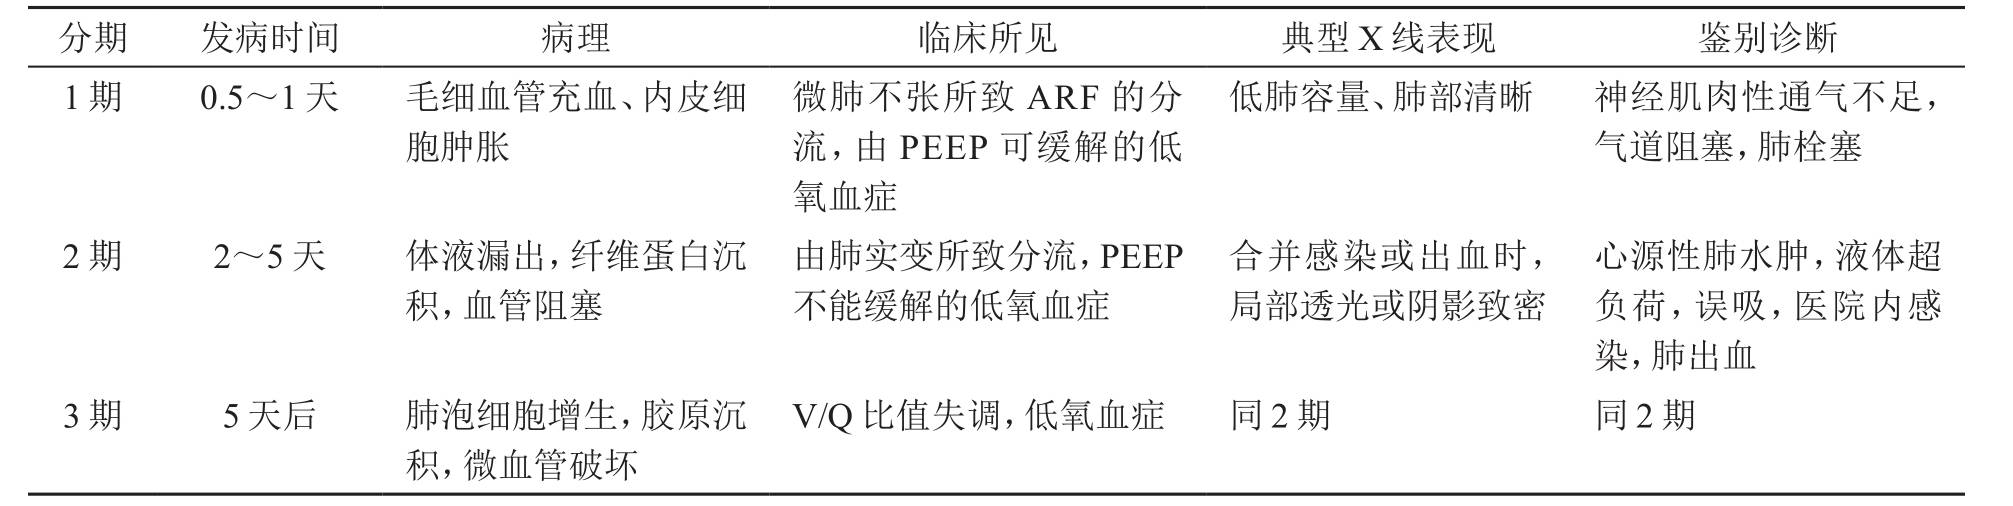
\includegraphics[width=6.69792in,height=1.67708in]{./images/Image00114.jpg}
\end{table}

\subparagraph{心源性肺水肿}

ARDS与心源性肺水肿的鉴别见下表\ref{tab29-2}。

\begin{table}[htbp]
\centering
\caption{ARDS与心源性肺水肿鉴别要点}
\label{tab29-2}
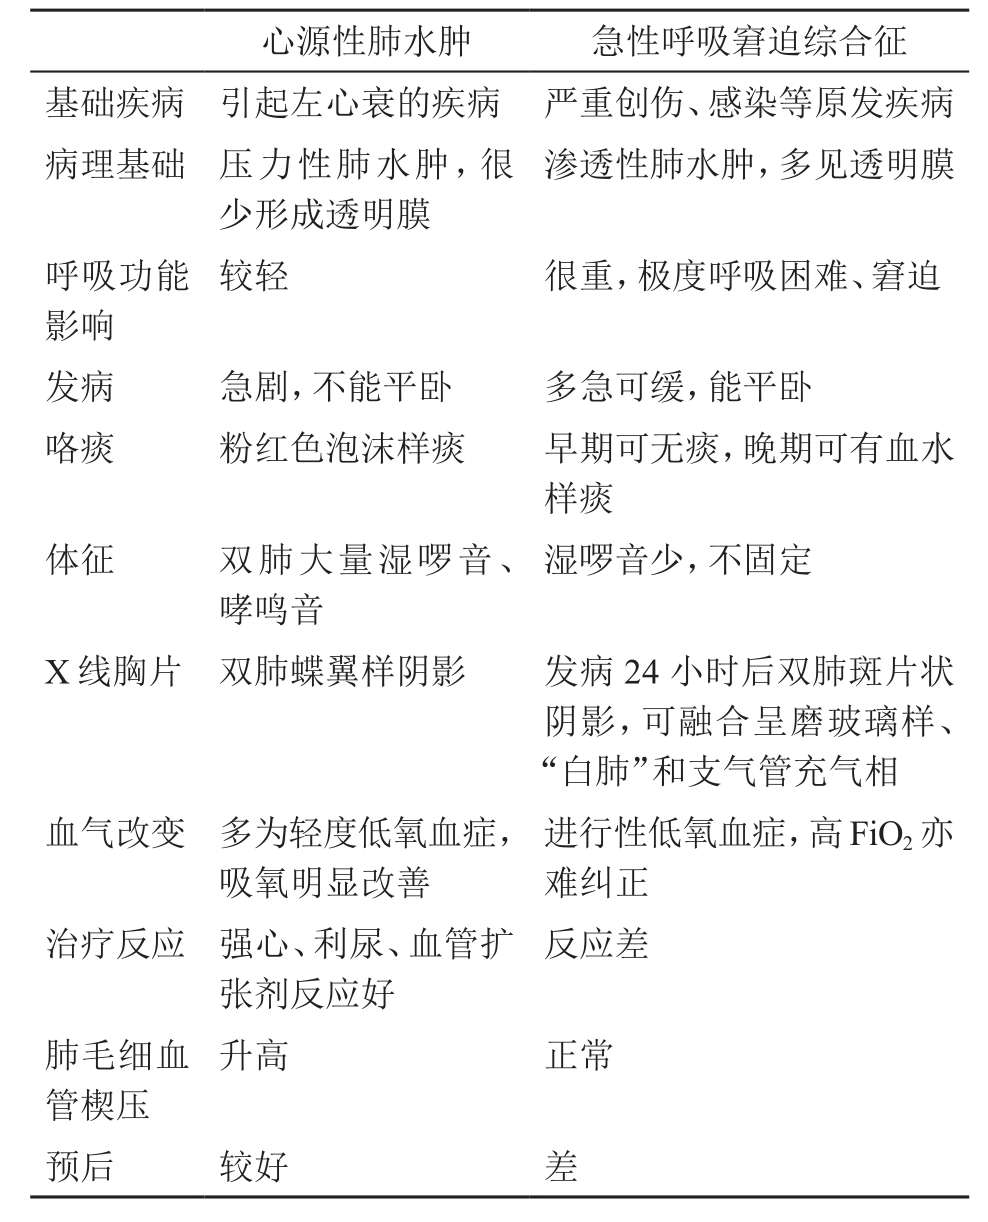
\includegraphics[width=3.28125in,height=4.0625in]{./images/Image00115.jpg}
\end{table}

\subparagraph{非心源性肺水肿}

有明确的大量输液、抽胸腔积液或气体过多、过快病史,肺水肿的症状。X线表现肺血管纹理增多变粗,蝴蝶状阴影典型表现多见于心脏病或尿毒症所致的肺水肿,治疗后消失也较快;低氧血症一般不重,吸氧后较易纠正。

\subparagraph{急性肺栓塞}

多骤然发病,呼吸急促,烦躁不安、咯血,发绀、较剧烈的胸痛。血气分析PaO\textsubscript{2}
和PaCO\textsubscript{2}
均降低,与ARDS颇为相似。实验室检查:肌酸磷酸激酶(CPK)、血清谷草转氨酶(SGOT)和乳酸脱氢酶(LDH)升高,X线胸片可见典型的楔形或圆形阴影、肺容量减少征象,如横膈抬高、肋间隙变小等,多伴有胸膜反应;可见肺动脉膨出。典型的心电图示Ⅰ导联S波加深,R波变小,ST段呈现J点降低,T波多直立。Ⅲ导联Q波变大、T波倒置(即SⅠQTⅢ改变)。选择性肺动脉造影和胸片并结合肺核素扫描,呈现被阻塞的肺动脉血管供血区放射性分布稀少或缺损,有助本病的确诊。

\subparagraph{特发性肺间质纤维化}

常为慢性过程,可呈亚急性或急性发展,表现为Ⅰ型呼衰,临床与ARDS表现相似,有主张应属ARDS者,但本病X线胸片呈网状、结节状或蜂窝状改变,病理基础与ARDS不同,总病程发展较ARDS缓慢,肺功能为限制性通气功能障碍为特征等可作鉴别。

\subparagraph{自发性气胸}

突发胸痛、呼吸困难、发绀,可通过病史、X线胸片、对氧疗的反应等予以鉴别。

\subsection{治疗}

ARDS起病急骤,发展迅速,损害广泛,预后差,病死率高。要求早期诊断、积极治疗,同时针对原发病处理以阻止病程的进展恶化,配合其他对症、支持治疗,才可以降低死亡率。目前的救治方法包括以下几个方面:

\subsubsection{原发病治疗}

1.严重创伤者及时处理外伤及止痛
、止血等;淹溺者迅速清除呼吸道积液及污物;大手术后患者注意引流管通畅等。

2.严重的感染既是
ARDS的高危致病因素,也是非感染病因导致ARDS后的最常见并发症和死亡原因。控制感染及预防院内感染是很重要的措施,明确感染部位,通过痰、血、尿等的细菌培养,检出致病菌,给予敏感抗生素治疗。未明确病原菌的情况下,可据病情经验选用抗生素,抗生素使用主张足量、联合、静脉给药,特殊情况可配合局部用药。

\subsubsection{机械通气}

机械通气是ALI/ARDS的关键性治疗措施,最近研究结果表明在ALI期即实施合理、有效的机械通气较易纠正低氧血症且对改善ARDS预后有显著的积极意义。

\subparagraph{通气方式的选择}

如病情处于ALI早期,无呼吸道阻塞,预计病情能够短期缓解的早期ALI/ARDS患者,可选无创密闭面罩方式施行正压通气,即无创机械通气(NIV)。NIV的好处是避免了与气管插管或气管切开相关的并发症,改善患者的舒适感,保留上气道的防御功能,保留了患者说话和吞咽功能,而且提供了建立和卸去机械通气的最大灵活性。采用无创通气的患者需神志清楚,能主动配合,气道分泌物不多,血流动力学稳定等。无创通气期间,除监测患者的气体交换反应外,还应监测以下的临床参数:主观反应(呼吸困难、舒适感和神志状态),客观反应(呼吸频率、心率和辅助呼吸肌的应用)、可能出现的并发症(腹部膨胀、面部皮肤压迫坏死、分泌物潴留)和腹肌的收缩(随过高吹起而活动)。2006年ALI/ARDS诊断治疗指南指出:ALI/ARDS患者在以下情况时不适宜应用NIV:①神志不清;②血流动力学不稳定;③气道分泌物明显增加而且气道自洁能力不足;④因脸部畸形、创伤或手术等不能佩戴鼻面罩;⑤上消化道出血、剧烈呕吐、肠梗阻和近期食管及上腹部手术;⑥危及生命的低氧血症。如NIV治疗1~2小时后,低氧血症和全身情况得到改善,可继续应用NIV。若低氧血症不能改善或全身情况恶化,提示NIV治疗失败,应及时改为有创通气。合并免疫功能低下的ALI/ARDS患者早期首先试用无创机械通气,可明显降低气管插管率、ICU病死率和住院病死率。

\subparagraph{通气模式的选择}

如采用无创面罩方式,常选压力支持通气(PSV)+持续气道正压(CPAP)、双时相气道正压(BIPAP)、双水平气道正压(BIPAP),同步间歇指令通气(SIMV)+
PSV
+呼气末正压(PEEP),如采用气管插管或气管切开套管方式通气,常选用连续强制通气(CMV)+
PEEP 或SIMV + PEEP +
PSV,压力调节容积控制通气(PRVCV),容积支持通气(VSV)以及液体通气(LV)等。当上述模式难于有效改善氧合或为达到更好人-机协调,还可采用以下模式:如高频正压通气、高频喷射通气、高频振荡通气。

\subparagraph{机械通气的辅助方法}

当采取上述方法难于有效改善氧合或为达到更好的人-机协调,可采用以下方式:①体外或肺外的气体交换:体外膜肺氧合、体外CO\textsubscript{2}
去除和腔静脉氧合。目的是让已受疾病损伤的肺充分休息,不再增加通气机所致损伤,并提供肺组织修复愈合的机会,但这些技术总的说来创伤较大,价钱昂贵,操作技术的专门性要求较高。由于体外膜肺氧合技术创伤大,对血流动力学影响严重,且减少肺血流影响肺组织愈合,故目前应用较多的是体外CO\textsubscript{2}
去除和腔静脉氧合;②俯卧位通气:俯卧位通气通过降低胸腔内压力梯度、促进分泌物引流和促进肺内液体移动,明显改善氧合。一项随机研究采用每天7小时俯卧位通气,连续7天,结果表明俯卧位通气明显改善ARDS患者氧合,但对病死率无明显影响。然而,若依据PaO\textsubscript{2}
/FiO\textsubscript{2} 对患者进行分层分析结果显示,PaO\textsubscript{2} /
FiO\textsubscript{2} <
88mmHg的患者俯卧位通气后病死率明显降低。可见,对于常规机械通气治疗无效的重度ARDS患者,可考虑采用俯卧位通气。但严重的低血压、室性心律失常、颜面部创伤及未处理的不稳定性骨折是俯卧位通气的相对禁忌证。此外还应注意在翻身过程中静脉内输液管和气管内插管的位置和通畅性。③液体通气:是指先将液体------全氟溴辛烷经气管内注入肺,然后进行正压通气。部分液体通气是在常规机械通气的基础上经气管插管向肺内注入相当于功能残气量的全氟碳化合物(如:全氟溴辛烷),可显著增加通气时O\textsubscript{2}
的摄取和CO\textsubscript{2} 排出,提高PaO\textsubscript{2}
,降低PaCO\textsubscript{2}
,增加肺顺应性,降低肺泡表面张力,促进肺重力依赖区塌陷肺泡复张。近期对90例ALI/ARDS患者的RCT研究显示,与常规机械通气相比,部分液体通气既不缩短机械通气时间,也不降低病死率,进一步分析显示,对于年龄<
55岁的患者,部分液体通气有缩短机械通气时间的趋势。因此部分液体通气可作为严重ARDS患者常规机械通气无效时的一种选择。

\subparagraph{机械通气策略在以下几方面较前有了新的转变}

①为减小肺泡跨壁压,避免肺泡过度扩张,改变以往的容积目标型(volume
targeted)为压力目标型(pressure
targeted)。临床上以气道平台压(Pplat)为指标,Pplat能够客观反映肺泡内压,其过度升高可导致呼吸机相关肺损伤。因此控制Pplat
< 30~35cmH\textsubscript{2}
O,可以减少气压伤的发生。2006年急性肺损伤/急性呼吸窘迫综合征诊断治疗指南推荐:在实施肺保护性通气策略时,限制气道平台压比限制潮气量更为重要。②避免肺泡过度扩张,降低潮气量,采用许可性高碳酸血症(permissive
hypercapnia,PHC)策略,PHC定义为:为避免气压-容量伤故意限制气道压或潮气量,允许PaCO\textsubscript{2}
逐渐增高> 50mmHg(容许二氧化碳逐步潴留,PaCO\textsubscript{2}
上升速度5~10mmHg/h,血pH亦适度降低)。近年RCT研究表明,ARDS通气时实施低通气和PHC肺保护策略明显降低患者死亡率。③通过改变呼吸时比的方法减低气道峰压(pip),提高气道平均压(paw)形成适当水平的内源性PEEP(PEEPi)改善氧合利于萎陷肺泡复张,减少肺泡表面活性物质丢失。④尽量减少机械通气的强制性,加强自主呼吸作用,促进人-机协调。⑤应用肺力学参数准确调整PEEP水平,寻找“最佳PEEP”,使之既可以防止呼气末肺泡萎陷(即所谓“肺开放”策略),又同时避免过度增加肺泡压。而Amoto及Villar的研究显示,在小潮气量通气的同时,以静态P-V曲线低位转折点压力+
2cmH\textsubscript{2}
O作为PEEP,结果与常规通气相比ARDS患者的病死率明显降低。因此在有条件情况下,应根据静态P-V曲线低位转折点压力+
2cmH\textsubscript{2}
O来确定最佳PEEP。⑥鉴于ARDS的肺损伤状态会随病程变化,强调动态呼吸监测,据以及时调整通气参数。

\subparagraph{主要通气参数调节范围为}

①吸入氧浓度(FiO\textsubscript{2} ):争取使长期FiO\textsubscript{2} <
0.6。②PEEP一般保持在5~15cmH\textsubscript{2}
O。目前多主张PEEP从低水平(3~5cmH\textsubscript{2}
O)开始渐增,至最佳PEEP水平(控制在10cmH\textsubscript{2}
O,一般不超过15cmH\textsubscript{2} O):SaO\textsubscript{2}
≥90\%,FiO\textsubscript{2} ≤0.6。如PEEP已> 15cmH\textsubscript{2}
O,而SaO\textsubscript{2} 仍< 90\%,则只可增加FiO\textsubscript{2}
,使SaO\textsubscript{2}
达90\%以上并稳定后,逐渐降低FiO\textsubscript{2}
,然后再降低PEEP,使之< 15cmH\textsubscript{2}
O,以巩固疗效。③潮气量(VT)选择:弃用传统的大潮气量(10~15ml/kg),目前推荐小潮气量通气(5~6ml/kg),在定容模式下应参考气道平台压(Pplat),使Pplat
< 30~35cmH\textsubscript{2}
O;VT的大小还需根据PEEP水平调整,PEEP水平高VT宜小,在小VT通气条件下,可适当增加呼吸频率来代保证分钟通气量,但呼吸频率增加不宜大于30次/分,否则亦易致肺损伤,此时可接受低通气状态,采取PHC策略,但PaCO\textsubscript{2}
不宜高于80~100mmHg,文献报道PaCO\textsubscript{2}
大多为50~100mmHg,最好在70mmHg以内,但pH不宜低于7.20,若PH <
7.20或者7.10时,大多数学者主张可适当补充碱,但顾虑补充碳酸氢盐后CO\textsubscript{2}
产生增加,有学者主张补三羟甲基氨基甲烷(THAM),也有学者不主张补碱。采取PHC时应注意排除颅内高压、严重心功能不全等禁忌证。

\subparagraph{呼吸机撤机方法}

病情得到控制后,FiO\textsubscript{2} < 0.5而PaO\textsubscript{2} >
60mmHg时开始减PEEP或CPAP,每次减2~3cmH\textsubscript{2}
O,间隔6~8小时病情稳定,减至2~0cmH\textsubscript{2}
O时(约需24~36小时),渐下调FiO\textsubscript{2}
至0.3,如PaO\textsubscript{2} >
60mmHg观察维持6~8小时病情稳定。可撤离呼吸机,撤机后留管观察2~4小时病情稳定可考虑拔管。

\subparagraph{机械通气过程注意事项}

机械通气中应加强气道管理,对于无脊髓损伤等体位改变禁忌证的机械通气的ARDS患者,体位应采用30°~45°半卧位,可显著降低机械通气患者呼吸机相关肺炎(VAP)的发生。机械通气时应用镇静剂可以缓解患者焦虑、躁动、疼痛,减少过度的氧耗,减少机械通气时间、ICU住院时间和总住院时间。但应先制定镇静方案,包括镇静目标和评估镇静效果的标准,根据镇静目标水平来调整镇静剂的剂量。但对机械通气的ARDS患者,不推荐常规使用肌松剂。危重患者应用肌松药后,可能延长机械通气时间、导致肺泡塌陷和增加VAP发生率,并可能延长住院时间。如确有必要使用肌松药物,应监测肌松水平以指导用药剂量,以预防膈肌功能不全和VAP的发生。应严密观察并避免并发症的发生,如肺气压容积伤(包括肺间质气肿、纵隔气肿、气胸、皮下气肿等)、低血压以及低心排量导致的心、脑、肝、肾等脏器灌注不足,呼吸性碱中毒,氧中毒,呼吸机相关肺炎等。

\subsubsection{改善血流动力学}

因ARDS患者的肺楔压较低,为了防止心输出量的降低,必要时需补充全血和电解质平衡液,使充盈压保持在15~18mmHg。如心脏指数(CI)下降,心脏收缩力降低时,可使用多巴胺、多巴酚丁胺等以增强其收缩力。合理地使用PEEP能产生最大的肺顺应性,对氧输送量和血流量的影响最小,Qs/Qt
< 15\%,FiO\textsubscript{2} >
0.5,而心输出量则无明显下降。ARDS患者因耗氧量增加,须增加组织的氧供(DO\textsubscript{2}
)和CI,并超过正常范围≥4.5L/(min•m\textsuperscript{2}
),DO\textsubscript{2} 须≥600ml/(min•m\textsuperscript{2}
)。故血流动力学监护时,可检测心输出量、肺动脉楔压和血气分析等。

适量补充以白蛋白为主高渗胶体液,可提高血浆胶体渗透压,有利于肺间质、肺泡水肿液的吸收,减轻肺水肿。ARDS时体液宜处于负平衡,可通过监测尿量、中心静脉压、肺小动脉楔压等,指导补液量,肺小动脉楔压(PAWP)维持在14~16mmHg。每日入液量一般应限制在2500ml以内,必要时可配合呋塞米静脉滴入利尿,利于肺水肿的吸收,并改善氧合。

\subsubsection{纠正酸碱和电解质紊乱}

与呼吸衰竭时的一般原则相同。重在预防。

\subsubsection{营养支持}

ARDS患者处于高代谢状态,急性期过后,恢复期的持续时间也往往较长,因而营养不良可使机体和免疫防御功能下降,易致感染和影响肺组织修复,故应及时补充热量和高蛋白、高脂肪营养物质。应尽早给予强有力的营养支持,鼻饲或静脉补给,保持总热量摄取83.7~167.4kJ(20~40kcal/kg),蛋白1.5~2g/kg,脂肪占总热量的20\%~30\%。

\subsubsection{药物治疗}

\hypertarget{text00078.htmlux5cux23CHP3-5-3-6-1}{}
(一) 肾上腺糖皮质激素

糖皮质激素主要作用有
:①可抑制花生四烯酸(AA)代谢,产生PLA\textsubscript{2}
抑制因子,从而抑制细胞膜上的磷脂代谢,减少AA的合成及TXA\textsubscript{2}
的产生;②抑制PMN、血小板聚集及微血栓形成;③具有广泛的抗炎、减轻毛细血管通透性等作用;④减少溶酶体酶及阻止单核巨噬细胞(MΦ)产生和释放TNF-α、IL-1等炎症介质的释放;⑤增加肺表面活性物质的合成,减轻微肺不张等作用。长期以来,大量的研究试图应用糖皮质激素控制炎症反应,预防和治疗ARDS。早期多项随机对照研究(RCT)观察了大剂量糖皮质激素ARDS的预防和早期治疗作用,结果糖皮质激素既不能预防ARDS的发生,对早期ARDS也没有治疗作用,反而可因继发感染、诱发上消化道出血、电解质紊乱而增加死亡率。但对于过敏原因(其血和肺泡灌洗液内有大量嗜酸性粒细胞,可能有嗜酸性粒细胞参与,或具有嗜酸性粒细胞肺炎的某些特征)、刺激性气体吸入(有些患者是在吸入可卡因后发生的综合征)、外伤骨折所致的脂肪栓塞、卡氏肺孢子虫肺炎等引起的ARDS,早期应用糖皮质激素治疗有效。此外感染性休克并发ARDS的患者,如合并肾上腺皮质功能不全,可考虑应用替代剂量的糖皮质激素。

持续的过度炎症反应和肺纤维化是导致ARDS晚期病情恶化和治疗困难的重要原因。糖皮质激素能抑制ARDS晚期持续存在的炎症反应,并能防止过度的胶原沉积,从而有可能对晚期ARDS有保护作用。小样本RCT试验显示,对于治疗1周后未好转的ARDS患者,糖皮质激素治疗组的病死率明显低于对照组,感染发生率与对照组无差异,高血糖发生率低于对照组。然而,最近ARDSnet的研究观察了糖皮质激素对晚期ARDS(患病7~24天)的治疗效应,结果显示糖皮质激素治疗{[}甲泼尼龙2mg/(kg•d),分4次静脉点滴,14天后减量{]}并不降低60天病死率,但可明显改善低氧血症和肺顺应性,缩短患者的休克持续时间和机械通气时间。进一步亚组分析显示,ARDS发病>
14天应用糖皮质激素会明显增加病死率。可见,对于晚期ARDS患者不宜常规应用糖皮质激素治疗。

\hypertarget{text00078.htmlux5cux23CHP3-5-3-6-2}{}
(二) 肺表面活性物质

ARDS患者存在肺泡表面活性物质减少或功能丧失,易引起肺泡塌陷。肺泡表面活性物质主要功能是减少肺泡和小气道内气-液界面的表面张力,据此改善肺顺应性、保持肺泡的稳定性、降低低肺容量位时的肺萎陷趋势,它可减少液体自毛细血管向肺泡的渗出及使呼吸机做功减少,还可减轻肺炎症反应,阻止氧自由基对细胞膜的氧化损伤,此外还有抗菌及免疫调节功能。并且大量的实验和临床证据表明在ALI时有表面活性物质的异常,主要不是数量的减少,而是功能的异常,提示补充肺泡表面活性物质替代疗法可以成为ARDS的治疗手段。目前国内外有自然提取和人工制剂的表面活性物质,可以通过气管内导管内以药液注入的方式或以气溶胶雾化吸入的方式给予。在治疗新生儿呼吸窘迫综合征(IRDS)有较好效果。最近一项针对心脏手术后发生ARDS补充肺泡表面活性物质的临床研究显示,与既往病例比较,治疗组氧合明显改善,而且病死率下降。目前肺泡表面活性物质的应用仍存在许多尚未解决的问题,如最佳用药剂量、具体给药时间、给药间隔和药物来源等。因此,尽管早期补充肺表面活性物质,有助于改善氧合,还不能将其作为ARDS的常规治疗手段。有必要进一步研究,明确其对ARDS预后的影响。

\hypertarget{text00078.htmlux5cux23CHP3-5-3-6-3}{}
(三) 吸入 NO

NO即血管内皮细胞衍生舒张因子,它能激活鸟苷酸环化酶(cGMP),使cAMP增加,从而有选择地舒张肺血管。NO分布于肺内通气良好的区域,可扩张该区域的肺血管,显著降低肺动脉压,减少肺内分流,改善通气/血流比值,并且可减少肺水肿形成,提高氧合指数,降低肺动脉压;NO与血红蛋白有高度的亲和力,可迅速与之结合而失活,故平均体动脉压和心排出量不变。有学者报道,将吸入NO与静脉应用阿米脱林甲酰酸(almitrine
bismyslate)联合应用,对改善气体交换和降低平均肺动脉压升高有协同作用。后者能使通气不良的肺区血管收缩,血流向通气较好的肺区;并能刺激周围化学感受器,增强呼吸驱动,增加通气;其可能产生的肺动脉压升高可被NO所抵消。Rossaint等使用低浓度(2~18ppm)NO吸入30分钟,每日一次治疗重症ARDS,疗程3~53天,7例全部被救活。也有临床研究显示,NO吸入可使约60\%的ARDS患者氧合改善,同时肺动脉压、肺内分流明显下降,对平均动脉压和心输出量无明显影响。但是氧合改善效果也仅限于开始NO吸入治疗的24~48小时内。并且NO开始作用及停止作用都非常迅速,突然停用NO时可出现反跳性血管收缩。高浓度的NO和它的微量氧化物(NO\textsubscript{2}
\textsuperscript{−} 和NO\textsubscript{3} \textsuperscript{−}
)对组织有极强的破坏作用,必须避免之,故吸入NO时,应使用标准空气(FiO\textsubscript{2}
=
21\%),通气流速5~20L/min,呼气与吸气比1∶3。然而两个RCT研究证实NO吸入并不能改善ARDS的病死率。因此吸入NO不宜作为ARDS的常规治疗手段,仅在一般治疗无效的严重低氧血症时可考虑应用。

\hypertarget{text00078.htmlux5cux23CHP3-5-3-6-4}{}
(四) 前列腺素 E1

前列腺素E1(PGE1)不仅是血管活性药物,还具有免疫调节作用,可抑制巨噬细胞和中性粒细胞的活性,发挥抗炎作用。但是PGE1没有组织特异性,静脉注射PGE1会引起全身血管舒张,导致低血压。静脉注射PGE1用于治疗ALI/ARDS,目前已经完成了多个RCT研究,但无论是持续静脉注射PGE1,还是间断静脉注射脂质体PGE1,与安慰剂组相比,PGE1组在28天病死率、机械通气时间和氧合等方面并无益处。有研究报道吸入型PGE1可以改善氧合,但这需要进一步RCT研究证实。因此,只有在ALI/ARDS患者低氧血症难以纠正时,可以考虑吸入PGE1治疗。

\hypertarget{text00078.htmlux5cux23CHP3-5-3-6-5}{}
(五) 山莨菪碱

山莨菪碱具有:①类阿托品结构,可阻滞胆碱能M受体,解除小血管痉挛,改善微循环V/Q比值,提高PaO\textsubscript{2}
,改善组织的DO\textsubscript{2}
;②抑制PMN和血小板聚集,减轻肺微血栓形成;③稳定溶酶体膜,减轻溶酶体酶对肺组织的损伤。应早期小剂量(10mg,每6小时缓慢静滴一次),病情改善后停用。

\hypertarget{text00078.htmlux5cux23CHP3-5-3-6-6}{}
(六) 己酮可可碱(pentoxifylline,PTX)

PTX是甲基黄嘌呤衍生物,为磷酸二乙酯酶的抑制剂,对ALI亦有较好的保护作用。通过降低PMN的黏附,能显著减轻肺内PMN聚集,减少肺血管渗出,有效地防止肺水肿形成。并可抑制IL-1及TNF激活PMN;还可改善肺灌注及氧运输,因此能减轻ALI和MODS。实验证明致伤前应用有明显预防低氧血症发生的作用,提示必须在ARDS发病的早期使用PTX才能收效。口服:100~200mg,一日3次,静滴:每日100~400mg,溶于250~500ml
5\%葡萄糖液中,90~180分钟静滴完毕。

\hypertarget{text00078.htmlux5cux23CHP3-5-3-6-7}{}
(七) 鱼油

鱼油富含
ω-3脂肪酸,如二十二碳六烯酸(DHA)、二十五烯酸(EPA)等,也具有免疫调节作用,可抑制二十烷花生酸样促炎因子释放,并促进PGE1生成。研究显示,通过肠道给ARDS患者补充EPA、γ-亚油酸和抗氧化剂,可使患者肺泡灌洗液内中性粒细胞减少,IL-8释放受到抑制,病死率降低。对机械通气的ALI患者的研究也显示,肠内补充EPA和γ-亚油酸可以显著改善氧合和肺顺应性,明显缩短机械通气时间,但对生存率没有影响。新进的一项针对严重感染和感染性休克的临床研究显示,通过肠内营养补充EPA、γ-亚油酸和抗氧化剂,明显改善氧合,并可缩短机械通气时间与ICU住院时间,减少新发的器官功能衰竭,降低了28天病死率。此外,肠外补充EPA和γ-亚油酸也可缩短严重感染患者ICU住院时间,并有降低病死率的趋势。因此,对于ALI/ARDS患者,特别是严重感染导致的ARDS,可补充EPA和γ-亚油酸,以改善氧合,缩短机械通气时间。

\hypertarget{text00078.htmlux5cux23CHP3-5-3-6-8}{}
(八) 氧自由基清除剂、抗氧化剂以及免疫治疗

根据ARDS发病机制,针对发病主要环节,研究相应的药物给予干预,减轻肺和其他脏器损害,是目前研究热点之一。

过氧化物歧化酶(SOD)、过氧化氢酶(CAT),可防止O\textsubscript{2}
和H\textsubscript{2} O\textsubscript{2}
氧化作用所引起的急性肺损伤;Becker报道低于生理浓度的血尿酸即可抑制O\textsubscript{2}
\textsuperscript{−}
、•OH的产生,还可清除次氯酸(HClO),因此,尿酸可能是目前发现最强有力的内源性氧自由基清除剂。维生素E具一定抗氧化剂效能,但会增加医院内感染的危险。

抗氧化剂N-乙酰半胱氨酸(NAC)和丙半胱氨酸(procysteine)通过提供合成谷胱甘肽(GSH)的前体物质半胱氨酸,提高细胞内GSH水平,依靠GSH氧化还原反应来清除体内氧自由基,从而减轻肺损伤。静脉注射NAC
对ALI患者可以显著改善全身氧合和缩短机械通气时间。

脂氧化酶和环氧化酶途径抑制剂,如布洛芬等可使血栓素A2和前列腺素减少,抑制补体与PMNs结合,防止PMNs在肺内聚集。

免疫治疗是通过中和致病因子,对抗炎性介质和抑制效应细胞来治疗ARDS,也是目前研究的热点,但这些免疫疗法大多尚处在实验阶段。目前研究较多的有抗内毒素抗体、IL-1受体拮抗剂(IL-1ra)、TNF-α拮抗剂(抗TNF-α抗体,抗TNF-α受体抗体,重组可溶性TNF-α受体)、自由基清除剂、花生四烯酸的抑制剂等。有些在动物实验中取得较好的效果,并开始进入临床研究阶段。

\subsection{预后}

ARDS的预后除与抢救措施是否得当有关外,常与患者原发病、并发症以及对治疗的反应有关。如严重感染所致的败血症得不到控制,则预后极差。骨髓移植并发ARDS死亡率几乎100\%。若并发多脏器功能衰竭预后极差,且与受累器官的数目和速度有关,如3个脏器功能衰竭持续1周以上,病死率可高达98\%。经积极治疗后,若持续肺血管阻力增加,提示预后不良。脂肪栓塞引起的ARDS,经积极处理,机械通气治疗可获得90\%存活。刺激性气体所致的急性肺水肿和ARDS,一般脱离现场,治疗及时,亦能取得较好的疗效。另外ARDS患者若经PEEP
0.98kPa(10cmH\textsubscript{2} O)治疗后,PaO\textsubscript{2}
有明显上升,预后较好。ARDS能迅速得到缓解的患者,大部分能恢复正常。

\subsection{预防}

对高危的患者应严密观察,加强监护,一旦发现呼吸频速,PaO\textsubscript{2}
降低等肺损伤表现,在治疗原发病时,应早期给予呼吸支持和其他有效的预防及干预措施,防止ARDS进一步发展和重要脏器损伤。

\protect\hypertarget{text00079.html}{}{}

\hypertarget{text00079.htmlux5cux23CHP3-5-6}{}
参 考 文 献

1. 中华医学会重症医学分会
.急性肺损伤/急性呼吸窘迫综合征诊断治疗指南.中华急诊医学杂志,2007,4

2. Eirini Kitsiouli,George Nakos,Marilena E. Lekka,et al.
Phospholipase A\textsubscript{2} subclasses in acute respiratory
distress syndrome. Biochimica et Biophysica Acta(BBA)-Molecular Basis
of Disease,2009,1792(10):941-953

3. François Lamontagne,Maureen O. Meade. Inhaled Vasodilators in ARDS
in ARDS:Do They Make a Difference? Evidence-Based Practice of Critical
Care,2010,131-134

4. Jiming Cai,Zhaokang Su,Yanping Zhou,et al. Beneficial effect of
exogenous surfactant in infants suffering acute respiratory distress
syndrome after cardiac surgery. European Journal of Cardio-Thoracic
Surgery,In Press,Corrected Proof,Available online 2 March 2011

5. Renee D. Stapleton,Julie M. Martin,Konstantin Mayer. Fish Oil in
Critical Illness:Mechanisms and Clinical Applications. Critical Care
Clinics,2010,26(3):501-514

\protect\hypertarget{text00080.html}{}{}

\hypertarget{text00080.htmlux5cux23CHP3-5-7}{}
附:2011欧洲重症医学会ARDS诊断标准

2011年
10月在德国柏林举行的欧洲重症医学会(ESICM)年会上,提出了新的ARDS诊断标准(ARDS柏林诊断标准),该标准主要从起病时间、低氧血症程度、肺水肿来源、X线胸片及其他生理学紊乱五个方面进行描述,见附表1。

ARDS柏林诊断标准有助于临床医师早期诊断、早期干预、早期判断疾病的严重程度,较为准确地估计预后。Gattinoni等对ARDS柏林诊断标准的准确性进行了验证,发现轻度ARDS患者的病死率为10\%,中度32\%,重度62\%。

附表1 2011欧洲重症医学会ARDS诊断标准

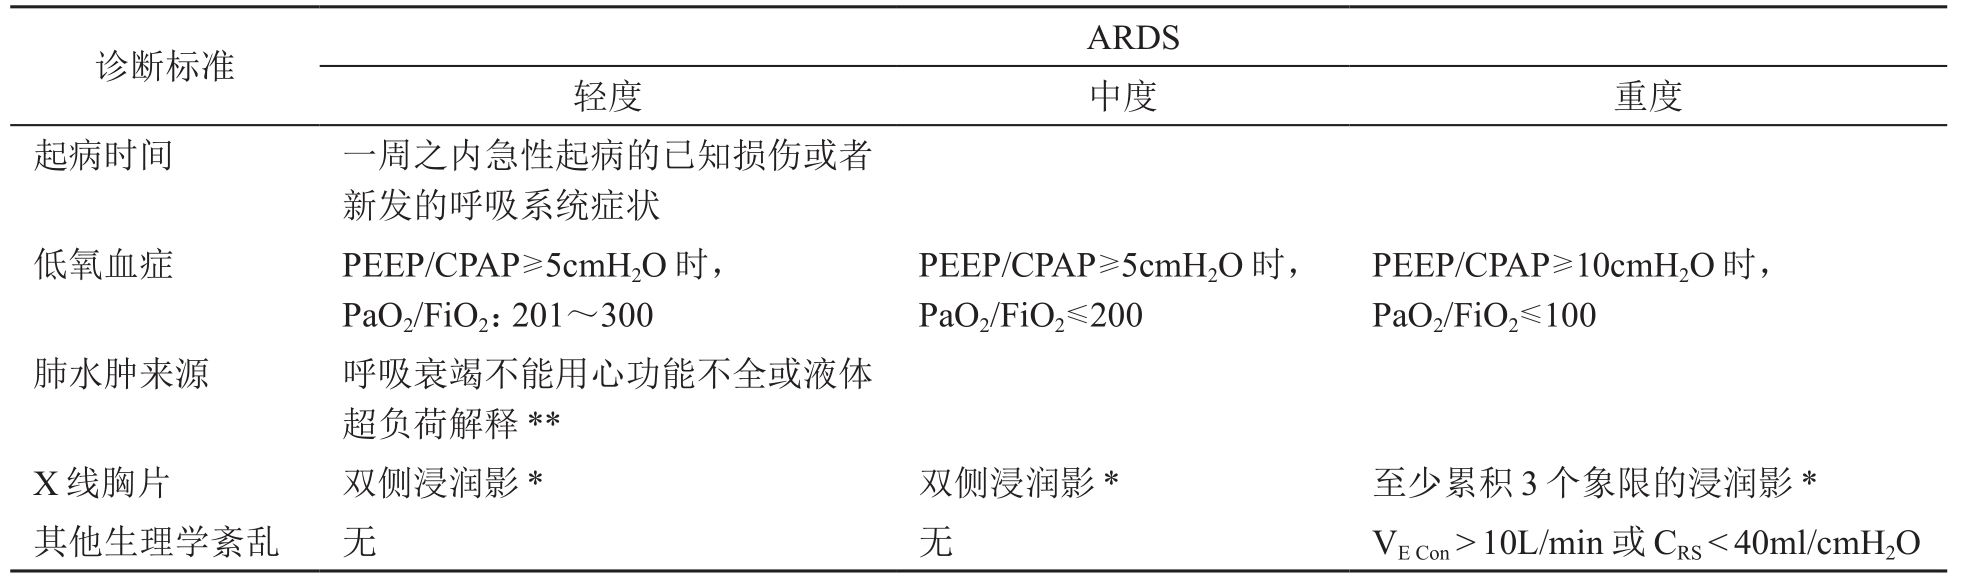
\includegraphics[width=6.57292in,height=1.94792in]{./images/Image00116.jpg}

*通过专业影像学培训,不能被胸腔积液、结节、肿块、肺叶塌陷所完全解释。

**如果没有危险因素,需要客观指标的评估。

V\textsubscript{E} \textsubscript{Con} = V\textsubscript{E} ×
PaCO\textsubscript{2} /40。

V\textsubscript{E} :呼出潮气量;C\textsubscript{RS} :呼吸系统顺应性

\protect\hypertarget{text00081.html}{}{}

\chapter{肝功能衰竭}

\section{概  述}

肝功能衰竭(liver
failure,简称肝衰竭)是指由多种因素引起的严重肝脏损害,导致肝脏本身合成、解毒、排泄和生物转化等功能发生严重障碍或失代偿,临床上出现以凝血机制障碍、黄疸、肝性脑病、腹水等表现的一组综合征。

1970年,美国Trey等首先提出暴发性肝衰竭(fulminant hepatic
failure,FHF)的概念,其临床特点为既往患者没有肝病史,现发生严重肝损害,并在出现首发症状8周内发生肝性脑病,而这些病变具有潜在可逆性。1986年,英国Gimson等提出了以急性肝衰竭(acute
hepatic failure,AHF)取代FHF的命名,并提出了迟发性肝衰竭(late onset
hepatic
failure,LOHF)的概念,其指急性肝脏病变起病8~24周内发生的肝性脑病。1993年,O'Grady等根据出现黄疸至脑病发生的间隔时间提出了一个新的分类法,即超急性、急性和亚急性肝衰竭3型:①超急性肝衰竭(hyperacute
liver
failure,HALF)指临床出现黄疸7天内发生肝性脑病者;②急性肝衰竭(acute
liver
failure,ALF)指临床出现黄疸8天~4周内发生肝性脑病者;③亚急性肝衰竭(subacute
liver
failure,SALF)指临床出现黄疸4周以上,12周以内发生肝性脑病者。1996年,在印度召开的国际肝病协会专题委员会(IASLS)上制定了统一的命名方案,将急性肝病引起的肝功能衰竭分为“急性肝衰竭(acute
hepatic failure,AHF)”及“亚急性肝衰竭(subacute liver
failure,SALF)”:AHF是起病4周内出现的肝功能衰竭,以肝性脑病为主要特征,其中起病10天内发生肝性脑病者称为超急性肝衰竭(hyperacute
hepatic
failure,HAHF),起病10天~4周发生肝性脑病者称为暴发性肝衰竭(FHF)。SAHF是起病4~24周出现的肝功能衰竭,以腹水和(或)肝性脑病为主要特征。这一分型将凝血酶原时间等纳入肝衰竭的诊断标准,肝性脑病不再作为唯一的诊断指标,但仍将具有慢性肝病史和组织学有慢性肝损害的患者排除在诊断之外。

2005年
,美国肝病学会(AASLD)在其颁布的急性肝衰竭处理指南中,将急性肝衰竭(ALF)定义为:原来没有肝硬化的患者,在发病26周内出现凝血异常(INR≥1.5)和不同程度的意识改变(肝性脑病)。肝豆状核变性、围产期获得HBV或自身免疫性肝炎患者可能已存在肝硬化,如发病<
26周,仍可纳入ALF范畴(曾经用于描述ALF的其他名词有:暴发性肝衰竭、暴发型肝炎、暴发性肝坏死等)。并指出,过去用于区分病程长短的名词(如超急性、急性和亚急性)已主张不用,因为这种方法并不能比病因具有更好的预后判断价值。然而,它仍然忽略了在慢性肝炎基础上发生肝功能衰竭的这一类群体。

中华医学会感染病学分会和中华医学会肝病学分会,于2006年制定并发布了我国第一部《肝衰竭诊疗指南》。在该指南中,根据病理组织学特征和病情发展速度,将肝衰竭可分为四类:

\subparagraph{急性肝衰竭(acute liver failure,ALF)}

急性起病,2周内出现Ⅱ度及以上肝性脑病并有以下表现者:①极度乏力,并有明显厌食、腹胀、恶心、呕吐等严重消化道症状。②短期内黄疸进行性加深。③出血倾向明显,凝血酶原活动度(PTA)≤40\%,且排除其他原因。④肝脏进行性缩小。

\subparagraph{亚急性肝衰竭(subacute liver failure,SALF)}

起病较急,15天~26周出现以下表现者:①极度乏力,有明显的消化道症状。②黄疸迅速加深,血清总胆红素大于正常值上限10倍或每日上升≥17.1μmol/L。③凝血酶原时间明显延长,凝血酶原活动度(PTA)≤40\%并排除其他原因者。

\subparagraph{慢加急性(亚急性)肝衰竭(acute-on chronic liver failure,ACLF)}

是在慢性肝病基础上出现的急性肝功能失代偿。

\subparagraph{慢性肝衰竭(chronic liver failure,CLF)}

是在肝硬化基础上,肝功能进行性减退导致的以腹水或门静脉高压、凝血功能障碍和肝性脑病等为主要表现的慢性肝功能失代偿。诊断要点为:①有腹水或其他门静脉高压表现。②血清总胆红素升高,白蛋白明显降低。③有凝血功能障碍,PTA≤40\%。

关于肝衰竭临床分期,《肝衰竭诊疗指南》根据临床表现的严重程度,SALF和ACLF可分为早期、中期和晚期:

1.早期
①极度乏力,并有明显厌食、呕吐和腹胀等严重消化道症状。②黄疸进行性加深,血清总胆红素≥171μmol/L或每日上升≥17.1μmol/L。③有出血倾向,30\%
<凝血酶原活动度(PTA)≤40\%。④未出现肝性脑病或明显腹水。

2.中期
在肝衰竭早期表现基础上,病情进一步发展,出现以下两条之一者:①出现Ⅱ度以下肝性脑病和(或)明显腹水。②出血倾向明显(出血点或瘀斑),且20\%
< PTA≤30\%。

3.晚期
在肝衰竭中期表现基础上,病情进一步加重,出现以下三条之一者:①有难治性并发症,例如肝肾综合征、上消化道大出血、严重感染和难以纠正的电解质紊乱等。②出现Ⅲ度以上肝性脑病。③有严重出血倾向(注射部位瘀斑等),PTA≤20\%。

2008年3月在韩国首尔召开第18届亚太肝脏研究学会(APASL)年会上,公布了慢加急性肝衰竭(acute
on chronic liver failure,ACLF)共识讨论草案,其主要内容如下:

1.ACLF概念
在慢性肝病(先前诊断或未诊断)基础上,因急性诱因作用,临床表现为黄疸和凝血障碍,4周内并发腹水和(或)肝性脑病。ACLF的临床亚型包括:①l
型ACLF:是指在发展为肝衰竭之前,虽有慢性肝病但肝功能代偿良好;②2型ACLF:是指在发展为肝衰竭之前,已经存在失代偿性肝硬化。

2.ACLF急性诱因的定义

(1)
感染性因素:①嗜肝或非嗜肝病毒;②乙型肝炎(显性或隐性)或丙型肝炎再活动;③其他影响肝脏的感染因素。

(2)
非感染性因素:①乙醇:4周内有饮酒史;②肝毒性药物,中草药;③自身免疫性肝炎或Wilson病发作;④静脉曲张出血(未达成共识);⑤外科手术。

(3) 未知的肝毒性因素。

3.ACLF慢性肝病的定义
慢性肝病包括:①所有病因引起的代偿性肝硬化;②慢性肝炎;③非酒精性肝病;④胆汁淤积性肝病和代谢性肝病。慢性肝病不包括脂肪变性。

4.ACLF定义 ①黄疸:血清总胆红素≥85μmol/L
(5mg/dl)和凝血障碍{[}国际标准化率(INR)≥1.5或凝血酶原活动度<
40\%{]}。②腹水和脑病:由体格检查确定。

5.慢加急性肝衰竭的临床表现
①肝功能异常:黄疸、低蛋白血症、腹水;②循环障碍:在ACLF中,肝硬化循环改变进一步加重。其中包括平均动脉压、全身血管阻力、肾血流量。一些分子吸附再循环系统(molecular
adsorbent recirculating
system,MARS)相关的研究证明可以引起通过有效地改善ACLF的血流动力学,提高患者生存率。③多器官衰竭:门体分流型肝性脑病;肝肾综合征(hepatorenal
syndrome,HRS)。④高病死率。

6.ACLF的鉴别诊断
①与急性肝衰竭相鉴别:急性肝衰竭是指预先不存在肝硬化的患者出现凝血异常(通常INR≥1.5)、不同程度的意识改变(脑病),疾病持续时间小于26周。Wilson病患者、垂直传播的获得性HBV感染者或自身免疫性肝炎患者尽管存在肝硬化的可能,但如果被诊断的时间小于26周,也可包括在ALF之内。②与失代偿性肝硬化相鉴别:慢加急性肝衰竭必须与慢性失代偿性肝病(即失代偿性肝硬化)进行区别。虽然两者均属于在慢性肝病基础上发生的肝衰竭,但两者的病程特点有明显区别。慢性失代偿性肝病表现为肝脏功能的进行性缓慢下降,直至不可逆性的肝衰竭。而慢加急性肝衰竭是指慢性肝病(通常是指肝硬化)患者在肝脏功能变化处于相对稳定的状态下,因各种急性损伤,如HBV突破、特异性免疫应答被激活、合并其他肝炎病毒感染、药物性肝损害、酒精性肝损害或身体其他部位的感染和炎症等,导致肝脏功能迅速恶化直至肝衰竭。

关于肝衰竭的病因,国内最常见的病因是肝炎病毒(主要是乙型肝炎病毒,尚有甲型、丙型、丁型、戊型肝炎病毒),其次是药物及肝毒性物质如抗结核药物(异烟肼、利福平等)、对乙酰氨基酚、抗代谢药物、毒蕈等。在欧美国家,药物是引起急性、亚急性肝衰竭的主要原因,以对乙酰氨基酚最常见;酒精性肝损害常导致慢性肝衰竭。儿童肝衰竭还可见于遗传代谢性疾病。

组织病理学检查在肝衰竭的诊断、分类及预后判定上具有重要价值,但由于肝衰竭患者的凝血功能严重降低,实施肝穿刺具有一定的风险,在临床工作中应特别注意。肝衰竭时(慢性肝衰竭除外),肝脏组织学可观察到广泛的肝细胞坏死,坏死的部位和范围因病因和病程不同而不同。按照坏死的范围及程度,可分为大块坏死(坏死范围超过肝实质的2/3),亚大块坏死(约占肝实质的1/2~2/3),融合性坏死(相邻成片的肝细胞坏死)及桥接坏死(较广泛的融合性坏死并破坏肝实质结构)。在不同病程肝衰竭肝组织中,可观察到一次性或多次性的新旧不一肝细胞坏死的病变情况。目前,肝衰竭的病因、分类和分期与肝组织学改变的关联性尚未取得共识。鉴于在我国以乙型肝炎病毒(HBV)感染所致的肝衰竭最为多见,因此以HBV感染所致的肝衰竭为例,各类肝衰竭的典型病理表现为:①急性肝衰竭:肝细胞呈一次性坏死,坏死面积≥肝实质的2/3;或亚大块坏死,或桥接坏死,伴存活肝细胞严重变性,肝窦网状支架不塌陷或非完全性塌陷。②亚急性肝衰竭:肝组织呈新旧不等的亚大块坏死或桥接坏死;较陈旧的坏死区网状纤维塌陷,或有胶原纤维沉积;残留肝细胞有程度不等的再生,并可见细、小胆管增生和胆汁淤积。③慢加急性(亚急性)肝衰竭:在慢性肝病病理损害的基础上,发生新的程度不等的肝细胞坏死性病变。④慢性肝衰竭:主要为弥漫性肝脏纤维化以及异常结节形成,可伴有分布不均的肝细胞坏死。

\hypertarget{text00081.htmlux5cux23CHP3-6-1-5}{}
参 考 文 献

1.
中华医学会感染病学分会肝衰竭与人工肝学组,中华医学会肝病学分会重型肝病与人工肝学组.肝衰竭诊疗指南.中华肝脏病杂志,2006,14:643

2. 丁义涛 .肝功能衰竭现代治疗学.南京:江苏科学技术出版社,2008

3. 王宇明
,张南.从慢加急性肝衰竭共识讨论到肝衰竭定义和分型诊断.中华肝脏病杂志,2008,16:404

4. 王英杰 .肝衰竭:定义、诊断与治疗.中华肝脏病杂志,

2008,16:725

5. Grady JGO. Acute liver failure. Postgrad Med,2005,81:148

\protect\hypertarget{text00082.html}{}{}

\section{急性肝功能衰竭}

急性肝功能衰竭(acute liver
failure,ALF,简称急性肝衰竭)是指原来不存在肝硬化的患者在一种或多种较强的致病因素作用下,引起的急性、大量肝细胞坏死,或肝细胞内细胞器严重功能障碍,在疾病发生的26周内出现肝功能迅速恶化,并导致精神异常及凝血障碍的一种临床综合征,具有较高的死亡率。急性肝衰竭的诊断标准中必备条件为:①凝血障碍,国际标准化比率(INR)≥1.5或凝血酶原活动度<
40\%;②精神异常即肝性脑病;③无肝硬化;④起病26周内。如果不能及时进行肝脏移植其病死率高达80\%~90\%。对于以下病例:如为Wilson病、母婴传播乙型肝炎或自身免疫性肝炎,尽管有肝硬化可能,只要本次起病<
26周,仍可诊断ALF。此外,对于发病前原有肝病处于相对静止阶段的慢性乙型肝炎的再活化或乙型肝炎基础上重叠丁型肝炎病毒感染(HDV)所致急性肝功能衰竭亦可纳入急性肝衰竭的诊断。

\subsection{病因与发病机制}

\subsubsection{病因}

可以导致急性肝衰竭原因较多。在这些原因中,既可以是一种因素致病,也可以是多种原因共同作用导致急性肝衰竭,在我国病毒性肝炎以及药物因素为最常见引起急性肝衰竭的致病因素。有15\%的急性肝衰竭的原因不清楚。

\subparagraph{病毒感染}

在我国的急性肝衰竭中,嗜肝病毒性感染所造成的肝炎占85\%~95\%,占急性病毒性肝炎的1\%~2\%。其中HBV、HCV、及HDV引起的急性肝衰竭相对较多,HAV及HEV引起者相对较少。急性乙型肝炎是病毒性急性肝衰竭最主要的原因,而HBV与HDV协同感染患者发生急性肝衰竭的危险性比单纯HBV感染者要高得多;同样地,HCV与HBV一样都是急性肝衰竭的常见病因,两者的协同感染引起急性肝衰竭的危险性较任何单一感染为高。HAV引起的急性肝衰竭仅约为0.1\%~0.01\%。在墨西哥、中美洲、印度中东区域内生活或旅行的妊娠妇女感染HEV后发生急性肝衰竭的几率可以高达20\%,但这一情况并不仅限于该地区,感染常发生在孕晚期,往往合并该病毒感染的孕妇病死率可达50\%以上。非嗜肝病毒感染引起的肝炎,以巨细胞病毒(CMV)性肝炎、EB病毒性肝炎及单纯疱疹病毒(HSV)性肝炎较常见,同样腺病毒、流行性出血热病毒、副黏液病毒也可以导致急性肝衰竭。常见的病毒感染病情危重程度常与年龄呈正相关性,但以青中年发病较多见。

\subparagraph{药物、毒物及化学物质}

在国外药物所导致的急性肝衰竭所占比例较大,在美国及欧洲发达国家是引起急性肝衰竭的主要病因,主要按照是否是对乙酰氨基酚所致分为:对乙酰胺基酚介导和非对乙酰氨基酚介导的肝衰竭,其中对乙酰氨基酚(扑热息痛)较多见,在美国的统计数据发病约达39\%。该药常见的治疗剂量为4g/d,如用药剂量超出治疗剂量极易发生急性肝衰竭,但对于酗酒患者应加以警惕,如对乙酰氨基酚摄入剂量<
4g/d时仍有个体出现肝脏功能衰竭。除此之外还有以下几类药物及毒素可以导致急性肝衰竭。①处方用药(往往和特异性体质所致的过敏反应机制有关),如:抗生素中的杀菌剂、抑菌剂(氨苄青霉素-克拉维甲酸、环丙沙星、强力霉素、红霉素、雷米封、呋喃妥因、四环素)、抗病毒药物、抗抑郁药(阿米替林、去甲替林)、降糖药(曲格列酮)、抗癫痫药物(苯妥英钠、丙戊酸盐)、麻醉剂(氟烷)、降血脂药(他汀类)、免疫抑制剂(环磷酰胺、甲氨蝶呤)、非甾体抗炎药及其他药物(双硫仑、氟他氨、金、丙硫氧嘧啶)。②违禁药品,如:致幻剂MDMA、可卡因。③中草药或其提取物,如:人参、薄荷油、石茧属植物。④一些与剂量相关的毒素,如:鹅膏属毒蘑菇、蜡样芽胞杆菌、蓝细菌毒素、有机溶剂(四氯化碳)、黄磷,这些毒素对致急性肝衰竭具有剂量依赖的特点。据美国1987~2006年的统计结果需要急诊肝移植的患者中常见的致病药物为呋喃妥因、苯妥英、丙硫氧嘧啶,由于存在药物使用后的个体差异,因此这类患者的发病存在致病药品广泛的特点,目前的研究结果显示药物介导的肝衰竭可能与患病个体存在易感基因有关,如阿莫西林介导的急性肝衰竭可能与谷胱甘肽S转移酶、特殊HLA基因型、超氧化物歧化酶基因多态性等有关。

\subparagraph{代谢异常}

急性妊娠脂肪肝所致的ALF仅次于药物性,本病多发生于妊娠后28周,个别报道可见到21周。Reye综合征为遗传性代谢疾病,有多种代谢紊乱,其中以脂肪代谢紊乱为主。肝豆状核变性(Wilson病)多呈慢性活动性肝病过程,但少数青少年患者可以急性肝衰竭为首发症状。其他可引起急性肝衰竭的代谢性疾病还有:α抗胰蛋白酶缺乏症、果糖耐受不良症、半乳糖血症、卵磷脂-胆固醇酰基转移酶缺乏症、酪氨酸血症等。

\subparagraph{缺血性肝衰竭}

多数情况下,肝缺血性损害仅见血清转氨酶升高及(或)轻度黄疸,仅在极少见的情况下,因极度缺血而又得不到及时纠正,才发展至急性肝衰竭,且常是多脏器功能衰竭(MOF)原因之一。除以上情况外,一些违禁药品如:MDMA、可卡因等可以导致肝脏缺血而引起急性肝衰竭。

\subparagraph{酒精中毒}

长期饮酒可以导致酒精性肝炎,在酒精性肝炎的患者中,轻的可以没有临床症状,严重的病例可以出现急性的肝脏功能衰竭而致患者死亡。

\subparagraph{严重感染、创伤}

对于一些严重感染性疾病和严重创伤的病例,当炎症反应明显不能被局限、组织坏死范围广泛时,感染和创伤所释放的毒素和炎症将向全身扩散,会出现全身脏器功能发生变化,最终发展为多脏器功能衰竭。肝脏往往是发生序贯脏器功能衰竭的上游脏器,在一部分严重感染和严重创伤的病例会出现急性肝衰竭为先导的多脏器功能衰竭(MOF)。

\subparagraph{自身免疫性疾病(自身免疫性肝炎)}

自身免疫性肝炎多数情况下是一种肝炎的慢性临床过程,25\%的患者临床表现为急性肝炎,且女性多于男性,病情严重者临床表现为凝血功能障碍、进行性加重的黄疸、腹水以及肝性脑病最终发展成为急性肝衰竭。

\subparagraph{血管因素}

血管因素所致的ALF临床并不少见,主要有以下几种情况:局限性缺血性肝炎、肝静脉血栓形成(Budd-
Chiari
syndrome)、肝静脉闭塞性疾病、门静脉血栓形成、肝动脉血栓形成(移植后)。

\subparagraph{恶性肿瘤浸润}

原发性肝肿瘤、广泛肝转移癌或腺癌浸润(乳腺癌、肺癌、恶性黑色素瘤、淋巴瘤及白血病)等,可以在原发病基础上发生急性肝衰竭。

\subparagraph{其他}

除上述原因外,还有以下原因可以引起急性肝衰竭:成人Still病、热休克、器官移植后的移植物抗宿主疾病(GVHD)、原发性移植肝无功能等。

\subsubsection{发病机制}

急性肝衰竭的发生和发展过程中,诱发病因不同,发生急性肝衰竭后临床病理生理过程也有所不同。按照肝脏功能损伤的机制可分为原发性肝损伤和继发性肝损伤。原发性肝损伤引起的肝衰竭依据病因不同起始损伤机制不同,主要通过直接或间接作用造成肝细胞大量坏死而最终发展至肝脏功能衰竭,原发性肝损伤所致的急性肝衰竭后期主要机制是前期损伤的基础上出现异常放大的、非特异的“瀑布样炎症介质反应”和不能被清除和代谢的毒素直接作用加速急性肝衰竭。继发性肝衰竭的发生机制相类似,主要是致病因素作用于机体后所产生的损害因素超出肝脏本身的处理能力,出现以下系列反应:单核-巨噬细胞系统受损,继之机体出现内毒素血症并激活细胞因子的释放机制而释放炎性细胞因子(TNF-α、IL-1、IL-2、IL-6、IL-8);同时体内的自由基介质(氧自由基、氮氧自由基)、脂质代谢产物(白三烯、血栓素、血小板激活因子、PGI\textsubscript{2}
)还有其他介质(如溶酶体酶、缓激肽、组胺、补体激活产物)在肝脏内明显增加,甚至扩散至全身而出现急性肝功能衰竭或MODS。

在病毒所致的急性肝衰竭中,病毒诱发急性肝衰竭的机制主要是病毒直接造成肝细胞表面结构改变或细胞破坏,在此基础之上诱发过度的免疫反应来清除病毒感染的肝细胞,使大量的肝细胞破坏溶解,当肝脏损伤达到一定程度并伴随着肝内库普弗细胞功能的衰竭时肝脏的解毒和机体清除介质、毒素能力将丧失,会加速肝细胞破坏和溶解的速度,在临床将表现为典型的急性肝脏功能衰竭。

药物、毒物及化学物质所诱导的急性肝衰竭机制较为复杂,原因有两个方面:其一是药物、毒物及化学物质的理化性质各异,造成急性肝脏损伤的机制不同;另一方面往往存在患者机体本身对所接触的药物、化学物质敏感性有所不同。后者发生急性肝衰竭主要机制是接触这些物质后出现超敏反应而造成急性肝衰竭。

在一些长期饮酒的患者中,如果因意外或故意超剂量服用了含对乙酰氨基酚类药品,将使这类患者发生严重的急性肝损伤乃至急性肝衰竭的危险性大大增加。除与药物自身毒性相关外,其主要机制是因为长期持续饮酒的患者肝内谷胱甘肽缺乏,超剂量服用含对乙酰氨基酚类药品将使肝内谷胱甘肽储备耗竭,谷胱甘肽含有一个活泼的巯基-SH,易被氧化脱氧,这一特异结构使其成为体内主要的自由基清除剂,在一部分敏感的患者中,当肝内谷胱甘肽被耗竭后可以使乙酰氨基酚相对安全的剂量(每天最大剂量4g)产生致死性的肝脏毒性作用,从而导致肝衰竭。

对于一些严重感染性疾病和严重创伤的病例,当炎症反应明显不能被局限、组织坏死范围广泛时,感染和创伤所释放的毒素和炎症将向全身扩散。在这过程中,除了致病病原体和严重创伤的本身对肝脏及全身的毒性作用外,还将通过炎症反应产生大量炎症介质(补体系统激活C3a、C3b、C5a、炎性细胞激活、TNF-α、IL-1、IL-6、IL-8、PA等),形成广泛、非特异、自身放大的病理过程,造成局部及全身炎性反应,当这些具有活性的炎性介质和炎症本身释放的自由基产生的量超出机体清除能力时,会出现全身脏器功能发生变化,会导致多脏器功能衰竭。肝脏作为单核-吞噬细胞系统的主要脏器之一,往往是发生序贯脏器功能衰竭的上游脏器,它的损伤和功能衰竭会促进和加重其他脏器功能的障碍和衰竭,所以在一部分严重感染和严重创伤的病例会出现急性肝衰竭为先导的多器官功能障碍综合征(MODS)。

自身免疫损伤的机制同造血干细胞功能相关,具有一定的遗传素质的人群中当一定外界因素作用于机体后,造血干细胞在其生长和发育过程中出现异常,其免疫活性成分(细胞免疫和体液免疫)将对自身的组织和系统出现识别错误,将其作为攻击目标造成损伤。自身免疫性肝炎基础上所发生的急性肝衰竭的主要致病机制是自身的免疫系统将肝脏作为攻击的靶器官,从而造成肝损伤,当病变过程发展较快、肝脏损害足够强烈时,临床上就表现为急性肝衰竭。一部分患者仅仅损伤肝脏,还有相当多的患者同时有其他肝外脏器及系统受累,在急性自身免疫性肝炎患者中的一部分可以由于治疗不当或合并其他因素出现肝损害的急性进展,从而发展成急性肝衰竭。

移植物抗宿主病(graft versus host
disease,GVHD)。是由于移植物的抗宿主反应而引起的一种免疫性疾病。所发生的急性肝衰竭虽然是免疫相关性肝损伤,但和自身免疫性肝损伤机制不同,效应细胞是移植物内的淋巴细胞进入宿主体内增殖并识别宿主肝脏组织细胞,进行免疫杀伤而最终造成急性肝衰竭。

\subsubsection{病理}

由于病因不同肝功能衰竭所致的病理改变有所不同,大体标本所见常常为肝脏缩小,重量只占正常肝脏重量的1/3~2/3,质地软,包膜皱缩。镜下有以下两种类型:Ⅰ型以大块肝细胞坏死,结构破坏消失为主要特征,肝脏细胞极度肿胀、肝细胞器如线粒体严重受损,残留肝细胞肿胀变性。坏死可在肝小叶中心区或呈弥漫性,也可呈相邻肝小叶的融合性坏死,广泛的坏死可引起小叶网状支架破坏,结构支架塌陷、小胆管增生、坏死区及汇管区炎细胞浸润。如果残存的肝细胞>
45\%存活的几率高;Ⅱ型以肝细胞微泡脂肪浸润(microvesicular fatty
infiltration)、肝细胞肿胀为主要特征,肝细胞坏死不明显,主要为肝细胞的细胞器衰竭,特殊染色可识别出脂肪浸润,无核移位,与细胞器功能衰竭所致的代谢障碍有关。无小叶肝细胞斑片状及大块坏死及汇管区炎细胞浸润。临床上血清转氨酶仅呈轻度增加,黄疸亦较Ⅰ型为轻。代谢性疾病所致的急性肝功能衰竭和急性妊娠期脂肪肝多见于此类型。上述病理改变系发生于原来健康的肝脏,如果致病因子不再持续作用,肝脏有可能通过再生得以复原。这就要求临床上尽早采取有效措施,以延长患者生命,为肝再生提供时间和条件。

\subsection{诊断}

\subsubsection{临床表现特点}

由于肝脏功能的复杂性,当出现急性肝衰竭时临床表现往往是以急性肝脏为主的消化系统功能衰竭的多脏器、系统功能不全综合征。肝脏及消化道功能障碍及衰竭的临床表现相对突出,除此之外可以见到消化系统以外的其他系统的功能障碍和衰竭的临床表现。

\hypertarget{text00082.htmlux5cux23CHP3-6-2-2-1-1}{}
(一) ALF一般状态及消化系统表现

\subparagraph{一般状态}

发生ALF的患者一般状态极差,全身体质极度虚弱、全身情况呈进行性加重、高度乏力、发热,同时由于炎症因子等作用出现全身炎症反应综合征,并处于高分解代谢状态。

\subparagraph{消化道症状}

恶心、呕吐、腹胀、顽固性呃逆、肠麻痹。急性期的患者较多合并消化道出血;黄疸,浓茶色尿,黄疸进行性加重,肝脏改变、肝功能异常,肝脏进行性缩小、ALT明显增高、胆-酶分离。黄疸出现后,消化道症状不仅不缓解,而且日趋增重。由于急性的肝脏肿大时肝被膜受牵拉,部分病例可见到剧烈腹痛,需同外科急腹症相鉴别。ALF的病程中可以有大量的腹水症和全身水肿,低蛋白血症是其主要原因,如有短时间快速进展的腹水症伴有腹痛的患者应警惕肝静脉血栓形成(Budd-Chiari
syndrome)。

\subparagraph{肝性脑病}

见于急性肝衰竭的所有病例。患者可有神志淡漠、性格改变、定向力异常,表现较重的有精神紊乱和昏迷,扑翼样震颤阳性,伴有黄疸进行性加重等。肝性脑病的具体分级详见本书第38章“肝性脑病”部分。随着肝性脑病的进行性加重及毒素等对脑星形细胞的作用,可出现脑水肿并可能进展为颅高压,临床上可表现为Cushing综合征、去大脑状态、强直、眼肌麻痹、瞳孔对光反射减退等。如急性肝衰同时合并重度肝性脑病、脑水肿、颅高压后死亡率亦会增高。

\subparagraph{黄疸}

黄疸在短期内迅速加深是其特征。每日上升的幅度,常超过34~51µmol/L(2~3mg/dl)。正常肝脏对胆红素的廓清有很大的储备能力,即使在急性溶血很明显时,其血清胆红素一般也不超过85µmol/L(5mg/dl),但在ALF患者,由于肝细胞的广泛坏死,廓清正常胆红素代谢的储备能力急剧下降,故短期内黄疸急剧上升。偶见ALF无明显黄疸时(主要见于Ⅱ型ALF),当出现意识障碍时常被误诊为精神病。

\subparagraph{无菌性胆囊炎}

超声检查可见胆囊增大,胆汁淤积,胆囊壁水肿明显。

\subparagraph{急性胰腺炎}

急性胰腺炎既可以是ALF的诱发因素,同时ALF也可以导致急性胰腺炎的发生,其中以对乙酰氨基酚介导的肝衰竭合并胰腺炎最为常见。其中有10\%
的ALF可以见到重症胰腺炎。并发急性胰腺炎后患者的死亡率也将大大增加。

\subparagraph{肝臭与肝脏进行性缩小}

肝臭的产生是由于含硫氨基酸经肠道细菌分解后生成的硫醇不能经肝脏分解而形成的特有气味,对临床诊断有提示作用。此外,肝脏的大小对ALF预后有重要意义,进行性缩小提示预后差,即使存活下来患者也可能直接进入肝硬化。

\subparagraph{代谢功能紊乱 :}

由于肝脏功能衰竭,肝脏解毒、清除能力明显下降,出现乳酸堆积、乳酸酸中毒,同时常常合并血氨明显升高。

\hypertarget{text00082.htmlux5cux23CHP3-6-2-2-1-2}{}
(二) 其他系统并发症

当
ALF发生其他脏器和系统并发症时,彼此间相互影响,一方面ALF加重其他系统的功能障碍和衰竭,另一方面其他系统的功能障碍和衰竭可以加速ALF的发展进程,致死率也明显增加。较常见的有:

\subparagraph{神经系统临床表现}

肝性脑病见于ALF的所有病例,ALF发生肝性脑病的时间各有不同,短的几天之内患者就可以进入肝昏迷状态。绝大多数的ALF患者可以见到脑水肿,因ALF死亡的尸检病例约51\%~81\%有脑水肿,常伴随肝性脑病发生。其中约25\%~30\%患者发生小脑扁桃体疝、颞叶钩回疝。由于脑水肿与肝性脑病的临床表现有许多重叠之处,肝性脑病可掩盖脑水肿的若干临床表现,如不提高ALF并发脑水肿的认识,极易漏诊。若患者已出现瞳孔、呼吸改变,抽搐或癫痫发作,已提示脑疝形成,多为晚期表现,诊断并不困难。对于ALF恢复的后期,如果肝脏功能及其他脏器情况均已经好转,患者仍有难以解释的意识障碍应警惕Wernicke脑病的发生。

\subparagraph{血液系统临床表现}

出血和出血倾向是ALF常见的突出表现之一,ALF患者早期即有出血倾向,表现为牙龈或口腔黏膜出血,鼻出血,球结膜出血,皮肤出血点或瘀斑。最早出现的往往是注射部位渗血。出血倾向常先于意识障碍的出现。大出血常发生于消化道,多见于疾病的中晚期,还有一些患者可以见到蛛网膜下腔及脑部等重要脏器出血。晚期ALF的大出血,除肝脏合成凝血因子减少外,还与其他凝血障碍有关:①DIC;②原发性纤维蛋白溶解:肝脏合成抗纤维蛋白溶酶功能减退,也不能清除纤维蛋白溶酶激活物,导致原发性纤溶;③血小板数量减少及质量下降;④毛细血管脆性增加;⑤胆汁淤积致胆盐排泄障碍使维生素K\textsubscript{1}
吸收障碍,继发维生素K依赖凝血因子合成障碍等因素。

\subparagraph{呼吸系统临床表现}

ALF时呼吸系统的变化也不少见,从低氧血症到呼吸窘迫综合征(ARDS)均可见到,约30\%的ALF发生ARDS。ALF时,舒张血管物质不能被肝脏摄取、灭能、大量入血循环,除引起外周血管阻力降低及低血压外,还引起肺内动静脉分流,致低氧血症,当肝脏功能衰竭时作为上游器官的单核-吞噬细胞系统被封闭,会使大量门静脉来源的内毒素及炎性介质通过肝脏而不被降解和灭活,直接进入肺循环,不仅造成分流加重,还会直接或间接损伤肺泡及间质导致ARDS。

\subparagraph{循环系统临床表现}

ALF的循环系统表现可有心律失常、心功能不全,心律失常主要有:心动过缓、室性异位搏动和房室传导阻滞。较常见的循环功能障碍是低循环阻力性低血压,临床病理生理状态是由此引起的器官组织灌注不良,甚至可以启动或促进加重急性肝功能衰竭的进程,80\%~90\%的ALF可出现低血压。收缩压≤80~90mmHg,常是预后不良的标志。低血压发生的机制较复杂,部分病例是由于毛细血管通透性改变的液体外渗及出血引起的血容量不足,或由于心功能不全,但其主要原因是外周血管阻力降低,其与下列因素有关:①血浆中假性神经递质取代真递质去氧肾上腺素;②循环内舒血管物质增多如一氧化氮、同位素毒素、胰高糖素、组胺、VIP等大量涌入血循环,这些舒血管物质使外周血管阻力降低;③细胞因子及内毒素血症:主要是细菌内毒素、肿瘤坏死因子(TNF-α)、白细胞介素1(IL-1)、白细胞介素6(IL-6)等,但这些因子在循环功能障碍中具体作用尚不完全清楚。

\subparagraph{泌尿系统临床表现}

泌尿系统并发症主要有肾功能不全、泌尿系统感染、出血等。肾功能不全的发生几率约70\%。少数病例归因于肾前性氮质血症,如消化道大出血、失水等。部分病例为急性肾小管坏死,大部分病例为功能性肾衰竭(肝肾综合征),内毒素血症和介质病是其主要形成机制。ALF一旦发生肾功能不全,会加重体内环境紊乱,也提示预后极差。ALF时因尿素氮合成降低,BUN不十分高,仅血清肌酐才能反映肾衰竭的严重程度。

\subparagraph{内分泌临床表现}

由于肝脏是糖、蛋白、脂肪等代谢的主要脏器,也是机体灭活各种激素的主要脏器,ALF发生时会出现较严重的内分泌紊乱:胃肠道激素、胰岛素、胰高血糖素、甲状腺素、肾素血管紧张素-醛固酮系统和抗利尿激素(ADH)等均有相应改变。其中主要的是低血糖症,40\%的ALF患者可出现空腹低血糖(2.22mmol/L)并陷入昏迷,有时与肝性脑病甚难鉴别,但补葡萄糖液后迅速好转,有学者称之为“假性肝昏迷”。ALF低血糖机制可能由于:①大量肝细胞坏死,致肝内糖原储备耗竭;②肝脏合成糖原分解酶如葡萄糖-6-磷酸酶的作用锐减,残存的肝糖原也不能分解为葡萄糖;③肝脏将非糖物质转化成为糖原(糖原异生作用)的功能衰竭;④高胰岛素血症等。

\subparagraph{水、电解质及酸碱平衡失调}

常见的有:

\hypertarget{text00082.htmlux5cux23CHP3-6-2-2-1-2-7-1}{}
(1) 低钠血症:

多表现为稀释性低血钠,病情愈重,稀释性低血钠愈明显。血清钠<
120mmol/L时,提示病情已属终末期。

\hypertarget{text00082.htmlux5cux23CHP3-6-2-2-1-2-7-2}{}
(2) 低钾血症:

常可使肝性脑病加剧,诱发心律失常。

\hypertarget{text00082.htmlux5cux23CHP3-6-2-2-1-2-7-3}{}
(3) 低血钙与低血镁:

也较常见,与摄取减少、腹泻、药物促进排除等因素有关。

\hypertarget{text00082.htmlux5cux23CHP3-6-2-2-1-2-7-4}{}
(4) 酸碱紊乱:

早期因过度换气致呼吸性碱中毒;低钾低氯致代谢性碱中毒;组织缺血缺氧,或肾功能不全致代谢性酸中毒;最后由于内毒素、脑水肿或并发呼吸道感染等原因引起呼吸中枢抑制,出现高碳酸血症时,则引起呼吸性酸中毒。

\subparagraph{并发感染}

ALF患者无论是否应用皮质激素,并发感染的发生率达50\%左右。常见感染部位为呼吸道感染、胆道感染、胃肠道感染、泌尿系统感染、自发性腹膜炎、败血症等。因为患者的极度虚弱,抵抗力低下易发生真菌和病毒等机会感染。ALF易并发感染的原因有:①肝脏清除抗原及毒性物质功能减弱。②ALF时,血浆中有抑制PMN单磷酸己糖旁路代谢活性的因子,还含有一种能减低PMN趋化性以及抗中性粒细胞正常趋化性的物质,再加上中性粒细胞Na\textsuperscript{+}
-K\textsuperscript{+}
-ATP酶活性减低,这些因素均使中性粒细胞丧失其防御感染的功能。③血浆补体及调理素降低。

\subsubsection{辅助检查}

ALF辅助检查对病因的诊断、病情评估、疗效评价和预后判断有重要意义。

\subparagraph{常规检查}

\hypertarget{text00082.htmlux5cux23CHP3-6-2-2-2-1-1}{}
(1) 血常规:

可见到血小板减少,其机制是DIC发生后造成的血小板消耗,合并细菌或病毒感染时可见到白细胞有增高和降低。

\hypertarget{text00082.htmlux5cux23CHP3-6-2-2-2-1-2}{}
(2) 尿常规:

可见到蛋白尿,肾实质损伤时有红、白细胞,尿胆原减少或消失,尿胆红素增加。

\hypertarget{text00082.htmlux5cux23CHP3-6-2-2-2-1-3}{}
(3) 便常规:

合并消化道出血时有便隐血阳性,急性期时大便可以呈白陶土便,为胆汁郁积所致。

\subparagraph{凝血检查}

ALF发生时会出现严重的凝血功能异常,是较为敏感的反映肝脏合成功能的指标。主要有凝血酶原时间测定;血小板计数与功能试验;各凝血因子和纤维蛋白原降解产物(FDP)测定等等。发病的数天后就可以见到凝血酶原时间延长及凝血酶原活动度下降,国际标准化比率(INR)≥1.5或凝血酶原活动度低于40\%考虑肝衰竭诊断成立。

\subparagraph{生化检查}

生化检查通过以下几个方面反映肝脏衰竭的情况:

\hypertarget{text00082.htmlux5cux23CHP3-6-2-2-2-3-1}{}
(1) 反映肝细胞损伤酶学指标:

血清酶检测包括丙氨酸氨基转移酶(俗称谷丙转氨酶,ALT)、门冬氨酸氨基转移酶(俗称谷草转氨酶,AST),ALT和AST能敏感地反映肝细胞损伤与否及损伤程度。其中,AST/ALT可以有助于预后判定,比值越高死亡率也随之增高,比值大于1时预后不佳。ALF后期酶学反而下降,与持续增高的胆红素相比呈“胆酶分离”现象,提示大量肝细胞死亡,预后极差。

\hypertarget{text00082.htmlux5cux23CHP3-6-2-2-2-3-2}{}
(2) 反映胆道功能状态的酶学指标:

主要有碱性磷酸酶(ALP)、γ-谷氨酰转肽酶(γ-GT或GGT)、总胆汁酸、5'{-}核苷酸(5'{-}NT)等。

\hypertarget{text00082.htmlux5cux23CHP3-6-2-2-2-3-3}{}
(3) 反映肝脏分泌和排泄功能的指标:

包括总胆红素(TBil)、直接胆红素(DBil)、总胆汁酸(TBA)等的测定。胆红素水平上升迅速和升高明显,急性期胆红素持续增高每日升高可达34.2~51.3μmol/L(2~3mg/dl),早期以直接胆红素为主,随后直接胆红素及间接胆红素双向增高。

\hypertarget{text00082.htmlux5cux23CHP3-6-2-2-2-3-4}{}
(4) 反映肝脏合成贮备功能的指标:

主要有前白蛋白(PA)、白蛋白(Alb)、胆碱酯酶(CHE)和凝血酶原时间(PT),也是通过检测肝脏合成功能来反映其贮备能力的常规试验,病情进展越快,持续时间越长,这些指标变化越明显。胆碱酯酶活性持续降低且无回升迹象,多提示预后不良。

\hypertarget{text00082.htmlux5cux23CHP3-6-2-2-2-3-5}{}
(5) 反映肝脏库普弗细胞功能的指标:

血清蛋白电泳中γ球蛋白增高提示库普弗细胞功能减退,不能清除血循环中内源性或肠源性抗原物质。

\hypertarget{text00082.htmlux5cux23CHP3-6-2-2-2-3-6}{}
(6) 反映肝细胞再生的指标:

主要是观察甲胎蛋白(AFP)水平变化,恢复期AFP水平升高提示肝细胞有再生,提示预后好。

\subparagraph{有关病因学检查}

对ALF的病因学检查很重要,和其治疗及预后密切相关。主要有:各种病毒学指标监测、药物的鉴定及血药浓度检测、血铜、毒物检测、自身免疫标志物、内毒素及补体等测定。其中一些影像学检查对病因的判定意义较大。

\subparagraph{其他生化检查}

血氨在ALF的患者增高较明显,其中以动脉血的血氨能更好地反映血氨的水平;血糖常常很低,反应糖原合成功能和糖原异生损害,严重时直接威胁患者生命;如果动脉血乳酸水平在ALF
4小时内超过3.5mmol/L或12小时超过3.0mmol/L提示为对乙酰氨基酚中毒所致急性肝衰竭,除此之外,还反映组织灌流减少和肝脏对乳酸清除能力减弱。血清肌酐水平可以反映肾脏功能变化情况,结合临床表现可以早期诊断肝肾综合征;血淀粉酶及脂肪酶的监测可以了解有无合并胰腺损伤;血清总胆固醇:常有胆固醇水平的降低,当小于1.56mmol/L时预后差。血氨和血支链氨基酸/芳香族氨基酸比例失调:血氨升高和血支链氨基酸/芳香族氨基酸比例由3~5下降至<
1;血气分析能发现酸碱失衡。

\subparagraph{影像学检查}

可以帮助诊断病因、了解肝脏储备功能、观察并发症及疗效评估等。常用的主要有:肝脏多普勒彩色超声、X线检查、CT及MRI。

\subparagraph{特殊检查}

一部分患者需要做以下特殊检查来判断和评估病情:肝脏活检、颅内压监测、脑电图。有条件均有必要开展上述检查。所有的患者应做心电图检查,进行心脏功能的动态监测,及时发现心律失常及低钾等心电图改变;血培养阳性时提示合并细菌感染或真菌感染。

\subsubsection{诊断注意事项及鉴别诊断}

ALF诊断过程中有以下三方面必须要关注:病史、神经系统症状及凝血异常出现的时间、辅助检查中重点关注出凝血情况。对于既往无肝病史(有肝病史者肝功能一直处于稳定状态)病史询问中有可引起肝损害的诱因,当患者肝功能严重受损,伴有高胆红素血症,PT明显延长,凝血酶原活动度小于40\%,如能排除慢性肝病,起病时间在26周以内出现肝性脑病即可诊断为急性肝衰竭。由于该病起病急,病程凶险,治疗强度要求高,且预后差,因此应注意和其他黄染及肝损伤疾病相鉴别。曾经用于描述ALF的其他名词有:暴发性肝衰竭、暴发性肝炎、暴发性肝坏死等。急性肝衰竭(ALF)的诊断名称已经包括所有的持续少于26周的肝衰竭。而过去超急性(<
7天)、急性(7~21天)和亚急性(> 21天但<
26周)等用于区分病程长短的诊断名词对疾病的发展和预后也无明显帮助,目前国际上建议以通用名称急性肝衰竭(acute
liver failure,ALF)可以很好描述这一疾病。

该病的鉴别诊断应基于病史、症状、体征及辅助检查几个方面来鉴别。需要鉴别的疾病主要是由黄疸、肝损害及精神症状的疾病,如急性黄疸型肝炎、慢性重症肝病、急性化脓性胆管炎、急性溶血性黄疸等。

\subsection{治疗}

急性肝功能衰竭的治疗应在生命支持治疗基础上进行对因治疗、处理及预防以消化道功能衰竭为主的多脏器功能障碍、终止肝损伤、促进肝细胞再生恢复生命功能为主要的治疗原则。

\subsubsection{一般治疗及护理}

\subparagraph{一般处理及护理}

一旦诊断急性肝脏功能衰竭应立即进行监护,在监护病房内实行专医专护、预防交叉感染、口腔护理、定时翻身;给予禁高蛋白饮食;保持大便通畅,此外,当诊断明确后应及早转诊至有监护及抢救条件的医院,并为肝脏移植做准备。

\subparagraph{生理需要支持治疗}

热量420~840kJ/d,静脉输入高糖(适量RI)防止低血糖发生;保证水、电解质平衡、量出而入;补充足够的维生素、微量元素;低蛋白血症时及时补充白蛋白。

\subparagraph{维持酸碱、水盐电解质平衡}

由于急性肝脏功能衰竭可产生较为复杂的酸碱、水电解质失衡,及时发现并治疗酸碱、水电解质失衡是治疗急性肝功能衰竭的重要环节。

\subsubsection{病因治疗}

由于ALF的病因对病情的发生、发展及预后有重要意义。不同病因在临床治疗也有着较大的差异。在明确病因的情况下,正确地对因治疗是取得理想临床效果的关键。常见的造成ALF病因治疗有以下治疗措施:

\subparagraph{乙酰氨基酚所致}

ALF的治疗
确诊或疑诊乙酰氨基酚过量导致的ALF患者,在摄入后1小时内的,如果量较大应立即洗胃以减少药物吸收。摄入药物在4小时以内的患者,应立即给予口服活性炭之后给予N-乙酰半胱氨酸(NAC)。用法:治疗开始时,140mg/kg口服,以后每4小时70mg/kg口服。若不能口服可静脉滴注,初始剂量为150mg/kg于15~60分钟内输入,以后持续泵入,4小时内给予12.5mg/(kg•h),此后为6.25mg/(kg•h)。血清药物浓度和转氨酶增高意味着即将或已经发生了肝损伤。对是否摄入了乙酰氨基酚的详细情况表述不清的ALF患者也尽早应用NAC。

\subparagraph{毒菌(蕈)中毒所致ALF的治疗}

明确或怀疑为菌(蕈)中毒的ALF患者,应考虑给予青霉素G(按每日30万~100万U/kg剂量)和水飞蓟宾(按每日30~40mg/kg剂量,维持3~4天)进行治疗。对明确菌(蕈)中毒导致的ALF患者,应该立即做肝移植准备,肝移植常为挽救此类患者生命的唯一选择。

\subparagraph{药物诱导性肝中毒所致 ALF的治疗}

对药物中毒的病例首先设法获得药物(含处方药物、非处方药物、中草药)的详细资料,如开始服用时间、服用剂量和最后服用的时间和数量及近1年来的食物等,尽量了解清楚摄入药物的成分。对于可疑药物性肝中毒导致ALF,立即停用所有的可疑药物并进行必要的药物治疗并寻找相应解毒剂。大多数药物中毒可以补充谷胱甘肽制剂,对乙酰氨基酚中毒应用葡醛内酯(肝泰乐)、还原型谷胱甘肽(泰特)、乙酰半胱氨酸等;酒精中毒补充足量的B族维生素;异烟肼中毒采用维生素B\textsubscript{6}
对抗。毒素中毒应用活性炭、血滤清除毒素。

\subparagraph{病毒所致肝衰竭}

在我国,乙型肝炎病毒(HBV)引起肝功能衰竭最为常见,占70\%~90\%。对HBsAg阳性(HBV
DNA复制≥1 × 10\textsuperscript{4}
)的肝衰竭患者,在知情同意的基础上应尽早给予核苷类似物如拉米夫定(lamivudine,LVD,100~150mg/d)或恩替卡韦(entecavir,ETV),并在化疗完成后继续维持6个月,以防止再活化和突发。肝衰竭抗病毒治疗需注意:①应在常规综合治疗的基础上使用抗病毒治疗;②应早期、及时应用有效的抗病毒药物,迅速有效地抑制HBV和改善肝功能和肝组织病变,才能减轻及阻断疾病的进展;③应选用强效、速效的抗HBV药物,首选LVD或ETV治疗。对慢性失代偿期乙肝肝硬化和慢性乙肝肝功能衰竭患者须长期治疗,不宜轻易停药;④对耐药的监测和防治:治疗过程中应定时监测耐药,发现耐药时,应及时加用或改用抗耐药的药物,如LVD耐药时可加用阿德福韦(adefovir,ADV)或改用ETV治疗。

明确或怀疑为疱疹病毒或水痘-带状疱疹病毒感染所致ALF,应该使用阿昔洛韦进行治疗。一般用30mg/(kg•d)静滴。

由于病毒感染所致急性肝脏损伤的患者发生机制和免疫紊乱有关,治疗过程中在不同阶段可以应用肾上腺皮质激素、胸腺素、干扰素。

\subparagraph{Wilson病所致ALF的治疗}

肝移植是这类患者的主要治疗措施,应明确诊断后在进行必要支持和对症处理的同时尽早作移植的准备。

\subparagraph{自身免疫性肝炎所致}

ALF的治疗
对疑诊自身免疫性肝炎所致ALF的患者,应进行肝活检以明确诊断。并给予激素治疗(泼尼松40~60mg/d)。激素治疗的同时,也应做肝移植的准备。

\subparagraph{妊娠急性脂肪肝}

/HELLP综合征所致ALF的治疗
对妊娠急性脂肪肝或HELLP综合征(溶血、肝酶增高、血小板降低),针对病因治疗的方案是创造手术条件,尽早终止妊娠。

\subparagraph{急性局部缺血性损伤所致}

ALF的治疗
对具有局部缺血性损伤证据的ALF患者,应加强支持治疗的同时尽早解决肝脏的缺血病因。

\subparagraph{Budd-Chiari综合征}

排除潜在的恶性肿瘤的患者,肝静脉血栓形成伴发肝衰竭应选择进行肝脏移植。

\subsubsection{保护肝脏功能、促进肝细胞再生治疗}

肝衰竭主要以肝细胞广泛坏死为其基本病理改变,预后主要取决于存活有功能的肝细胞数量和残留肝细胞的再生能力。因此,阻止肝细胞坏死,促进肝细胞再生是决定治疗成功与否的关键。常用药物有:

\subparagraph{促肝细胞生长因子(HGF)}

HGF具有促进肝细胞的再生、阻断自由基的脂质过氧化、抑制肿瘤坏死因子活性、阻止肝细胞坏死、增强库普弗细胞的吞噬功能、保护肝细胞等作用,宜尽早应用。用法:HGF
80~100mg/d加入10\%葡萄糖液250ml中静滴,疗程视病情而定。

\subparagraph{前列腺素 E(\textsubscript{1} PGE\textsubscript{1} )}

PGE\textsubscript{1}
可改善肝脏血流,保护肝细胞、促进肝细胞再生、防止肝细胞坏死,稳定肝细胞膜,减少毒性物质积蓄,给肝细胞创造一个良好的再生环境。用法:PGE\textsubscript{1}
200μg/d加入10\%葡萄糖液250ml中静滴,10~15天为一疗程。

\subparagraph{高血糖素 -胰岛素疗法(G-I疗法)}

以5\%葡萄糖液中加正规胰岛素10U和高血糖素1mg,静滴,持续2小时,每日1次。G-I疗法的机制,一般认为高血糖素作用于受体而激活腺苷酸环化酶,使细胞内cAMP浓度增加,后者又激活组蛋白激酶使染色体中组蛋白去阻遏,促使mRNA转录,增加酶和蛋白质的合成,促进肝细胞再生。胰岛素虽可使cAMP减低,但可促进蛋白质合成中的转录进程,并可促使线粒体生成ATP。两者合用对肝细胞再生有协同作用。近年来有学者观察到G-I疗法的治疗作用与改善氨基酸失衡有关。

\subparagraph{甘草酸制剂}

这类药物主要成分为甘草酸(甘草甜素),并含有一部分的半胱氨酸和甘氨酸。具有类肾上腺皮质激素作用,无明显的激素副作用;能利胆、解毒、抑制体内自由基的产生和过氧化脂质的形成,具有降黄疸和氨基转移酶的作用。

\subparagraph{门冬氨酸钾镁}

该制剂含天门冬氨酸、钾离子、镁离子等。天门冬氨酸在人体内是草酰乙酸的前体,在三羧酸及鸟氨酸循环中起着重要作用,使氨(NH\textsubscript{3}
)与二氧化碳生成尿素有去氨作用。钾离子是细胞生命所必需,是高能磷酸化合物合成分解的催化剂。镁离子是生成糖原及高能磷酸键不可缺少的物质,是糖代谢中多种酶的激活剂,也能使血管扩张,有利于肾血流量,利尿,降低颅内压,增加脑组织的血液循环,改善代谢,还可增强门冬氨酸钾盐的治疗效应。常用量为20~40ml/d,加入10\%葡萄糖溶液200~400ml中静滴。

\subparagraph{中药制剂}

常用的有苦黄、茵栀黄、丹参注射液。苦黄注射液具有利湿退黄、清热解毒的作用。用法:苦黄注射液30~60ml加入5\%~10\%的葡萄糖液250~500ml中静脉滴注。茵栀黄注射液具有清热、解毒、利湿、退黄作用。茵栀黄注射液10~20ml溶于10\%葡萄糖液250~500ml中静脉点滴,每日1次。丹参通过改善肝内微循环提高库普弗细胞功能、降低肝门静脉压力、调节免疫功能、促进肝细胞再生、抗肝纤维化等起到护肝的作用,但有出血的情况应避免应用。用法:复方丹参液10~20ml,加入5\%~10\%葡萄糖液中静脉点滴。但以上药物治疗ALF主要作为辅助用药。

\subparagraph{去氨治疗及维持支链氨基酸/芳香族氨基酸比值}

可应用谷氨酸钠23g/d,精氨酸20g/d,但应注意电解质及酸碱平衡;维持支链氨基酸/芳香族氨基酸比值应用富含支链氨基酸的肝用氨基酸,以静脉滴注为主,也可以口服。

\subsubsection{系统功能支持治疗}

\subparagraph{肝脏功能支持}

ALF时暂时性肝支持疗法(temporary hepatic
support)或称人工肝支持系统(artificial liver support
system,ALSS)是借助体外机械、化学或生物性装置,暂时或部分替代肝脏功能,从而协助治疗肝脏功能不全或相关疾病。由于肝脏损伤后具有较强的再生功能,通过暂时的功能替代可以使患者争取到足够长的生存期,然后通过肝再生而恢复肝脏功能。传统上按照人工肝组成及性质分为非生物型人工肝、生物型人工肝及组合型生物人工肝,是通过血液透析、血滤、血滤透析、血浆置换、复合性非生物人工肝支持系统(如系统化的人工肝支持ALSS)、离体肝灌流和血浆分离等连续性血液净化技术,对体内的毒素、炎性介质、代谢产物等进行清除以达到解毒的目的,以人工培养的肝细胞为基础构件组成体外生物反应系统。它不仅具有肝脏的特异性解毒功能,还可以参与能量代谢,具有生物合成转化功能,分泌促肝细胞生长活性物质等。尽管人工肝技术发展较快,但要设计出可以真正替代功能复杂接近人体肝脏功能的人工肝脏还有一段很长的路要走。

\subparagraph{胃肠功能支持}

在一定程度上是各种综合护肝治疗的基础。保护好胃肠功能,可以减轻和防止肠源性细菌、内毒素及肝脏损害物质经门静脉途径进一步造成肝脏功能损害,同时也可以达到预防和治疗肝性脑病的目的。临床主要措施有:给予禁高蛋白饮食;保持大便通畅,酸化肠道(全肠道)、清除肠道毒素及杂质(投给乳果糖、微生态制剂),乳果糖以保证每日大便1~3次即可,细菌制剂可以加量投给,如排便不通畅时可以应用大黄粉或浸液,当排便次数过多时,给予蒙脱石散(思密达)加强肠道黏膜保护,防治细菌及毒素移位。

\subparagraph{维持酸碱、水盐电解质平衡}

由于急性肝脏功能衰竭可产生较为复杂的酸碱、水电解质失衡,及时发现并治疗酸碱、水电解质失衡是治疗急性肝功能衰竭的重要环节。

\subparagraph{出凝血功能支持}

纠正出凝血机制异常预防及治疗出血应贯穿于整个抢救治疗的始终,和其他的脏器功能支持治疗同样重要。由于肝脏功能衰竭时凝血因子及纤维蛋白原产生障碍,应及时输注新鲜血及血浆,补充凝血酶原复合物(PPSB)及纤维蛋白原(血纤维蛋白原低于1g/L时应用);给予各种止血剂,如维生素K、肾上腺色腙(安络血)、酚磺乙胺(止血定)、注射用血凝酶等,始终使出凝血系统处于一个相对的稳态;一旦发生消化道出血应立即给予制酸剂、去甲肾上腺素冰盐水、云南白药、凝血酶、胃黏膜保护剂,及时控制出血。

\subparagraph{神经系统功能支持}

目前对于肝性脑病、脑水肿、颅高压的发病机制尚不是十分明确,可能是肝衰竭后毒素清除功能下降,大量毒素蓄积,影响神经递质的合成及释放、影响脑细胞线粒体功能、出现神经元氧化性应激、导致星形细胞渗透压屏障障碍而终于出现星形细胞水肿,就目前研究结果而言,明确与肝性脑病发病呈正相关的毒素为血氨,且血氨值越高脑病程度越重。因此治疗重点是预防和治疗肝性脑病、纠正脑水肿、防止Wernicke脑病的发生。针对肝性脑病治疗的关键是通过综合治疗手段去除可以引起肝性脑病加重的各种因素,同时应加强维护胃肠功能,减少肠源性毒素产生并促进其排除,除此之外针对肝衰竭所致脑功能异常还可以给予以下治疗措施:

(1)
去氨治疗:常用药物有鸟氨酸-门冬氨酸二肽治疗,每日常规剂量是20g静脉滴注治疗,但该药物的治疗对亚急性及慢性肝衰竭患者疗效确切,对于急性肝衰竭患者尚缺乏循证医学证据;鸟氨酸-α-酮戊二酸,但疗效不及前者;谷氨酸钠或钾,给予这两种药物治疗时应注意电解质及水潴留的情况;临床上较为常用的还有精氨酸20g/d静脉滴注治疗肝性脑病。如患者神志情况允许,可给予口服乳果糖治疗,如脑病情况较重可考虑鼻饲给药,同时应加强灌肠清理肠道治疗,并可考虑给予利福昔明以减少肠道产氨。如上述治疗疗效欠佳时可考虑应用肾脏替代治疗及亚低温治疗。

(2)
纠正芳香族及支链氨基酸的不平衡:临床给予富含支链氨基酸口服和静脉滴注,该治疗除了纠正氨基酸代谢失平衡外,还可以纠正胰岛素和胰高血糖素紊乱所致的高血糖,同时也有促进正氮平衡去氨的作用。

(3)
促醒治疗:苏醒剂可以用醒脑静20~40ml静脉滴注;GABA/BZ复合受体拮抗剂有荷包牡丹碱(bicuculline)、氟马西尼(flumazenil)0.5mg加生理盐水10ml静脉推注后,用1mg加入到生理盐水中30分钟内静脉滴注或泵入。

(4)
对于脑水肿首先应注意防止低钠血症,目前多中心研究结果表明,对肝性脑病患者应用高渗盐水能够延迟脑水肿发病,为急诊进行肝移植治疗提供先决条件。对有明确证据的脑水肿患者应考虑进行颅内压监测,并维持患者ICP值<
20mmHg,如患者ICP >
20mmHg且肾脏功能正常可给予甘露醇脱水治疗,但该药物治疗的疗效并不十分确切,约有50\%左右的患者脱水效果并不理想,因此在用药过程中应严密监测患者的治疗反应,此外对于血浆渗透压>
320mmol/L及ICP >
60mmHg的患者甘露醇的治疗效果均不理想,应慎重给药。如患者肾脏功能异常时可考虑甘露醇及肾脏替代治疗同时进行,以期获得良好的疗效。近期对于等待进行肝移植的患者进行32~33℃的低温治疗的临床研究显示能够有效的控制脑水肿,但随之而来的问题包括凝血功能异常加重、增加感染风险、影响肝脏再生功能等等,因此到目前为止尚未将低温治疗纳入治疗指南。此外适当给予山梨醇、纠正低氧血症、肾上腺皮质激素等治疗均可在一定程度上控制脑水肿。

(5)
Wernicke脑病治疗重点在预防:治疗过程中应注意补充大量富含B族的维生素。

(6) 低血糖性意识障碍:约40\%的ALF患者血糖<
2.22mmol/L(40mg/dl),在儿童病例更易发生。ALF的患者意识状态突然发生改变时应立即作血糖检测以除外低血糖可能。低血糖可导致肝性脑病,也可使脑功能发生可逆性或不可逆性损伤,治疗措施是立即给予葡萄糖。

\subparagraph{维持肾功能}

ALF发生的过程中,主要以MODS为主要临床特征,最常伴随出现的是肾脏功能不全。主要治疗措施有调整液体量、避免损伤肾脏药物、预防和治疗内毒素血症等。对于严重的病例适时采用连续性肾脏替代(CRRT)治疗,CRRT治疗不但可以清除体内多余的水分,维持机体的水盐代谢平衡,还可以对炎症介质有清除作用,一般采用高分子合成膜用高流量行CRRT,可以清除IL-1、血小板活化因子及部分补体。在进行CRRT治疗时由于患者凝血功能存在或存在潜在异常风险,因此推荐枸橼酸抗凝而不是常规的肝素抗凝策略。由于CRRT后组织间的水肿减轻,组织细胞的氧输送改善,组织缺氧所致的炎症介质释放也将明显改善。适时应用CRRT可以提高ALF患者的抢救成功率及生存率。

\subparagraph{循环功能支持}

ALF的循环功能障碍时,一旦出现循环功能障碍,应在有血流动力检测情况下,首先应给予积极的容量复苏,使CVP达8~12mmHg;监测ScvO\textsubscript{2}
或SvO\textsubscript{2}
,若未达到0.70,则应根据血红蛋白浓度,输注浓缩红细胞使血细胞比容达到0.30以上;若ScvO\textsubscript{2}
或SvO\textsubscript{2}
仍未达到0.70,应给予多巴酚丁胺{[}最大剂量至20μg/(kg•min){]}以达到恢复循环功能的目的。其他常用的血管活性药物还有多巴胺、去甲肾上腺素、米力农等。

\subparagraph{呼吸功能支持}

呼吸功能障碍或衰竭在ALF并不少见,除针对原发病治疗减轻肺损伤外,临床主要对呼吸功能衰竭的患者给予机械通气支持治疗。

\subparagraph{抗炎治疗}

目前对于是否进行预防性的抗感染治疗尚存在争议,对于怀疑感染的病例应积极寻找病灶、确定病原菌。对于发生的感染,抗生素选择时应考虑其敏感性、肝毒及肾毒性等。

\subparagraph{激素治疗}

由于相当一部分ALF患者的发病机制是由于机体过度的炎症介质反应所致,这类患者应用肾上腺皮质激素可以抑制过度的炎症反应,防止炎症介质加重肝脏及全身脏器系统的损伤及功能障碍。但由于激素带来益处的同时还伴随着一定的副作用,如增加感染概率、感染扩散等。临床应用时机和剂量应根据具体患者的情况而定,没有固定的指南可以遵循。

\subsubsection{肝移植治疗}

肝移植技术是目前唯一明确有确切疗效的急性肝衰竭的治疗策略,随着治疗水平及技术的进展,手术后存活率明显升高,甚至有报道称术后1年生存率可达80\%以上。人工肝技术结合肝移植技术联合治疗模式使ALF的治疗水平有了新的提高。对于急诊医师在处理急性肝衰竭的患者时将面临两个难以抉择的困境,其一为是否对患者进行急诊肝移植治疗,因为这个决定可能错误的使本不需要肝移植就能够自行恢复的肝衰竭患者接受不必要的手术治疗,并且此后终生进行免疫抑制治疗,增加了感染的发病率及死亡率;其二为何时为肝衰竭患者进行急诊肝移植治疗,虽然尽早对需要手术的患者进行移植能够改善死亡率,但是过早的手术使得手术前的准备配型工作不能充分进行,使手术后并发症发病率明显升高,严重影响手术后死亡率。目前被广泛接受及使用的指征是King's
College标准:对乙酰氨基酚相关的肝衰竭患者需满足以下标准:pH <
7.3(充分液体复苏治疗),Ⅲ期以上的肝性脑病,Scr > 300μmol/L,INR >
6.5;非对乙酰氨基酚相关的肝衰竭患者标准如下:任意级别肝性脑病+ INR >
6.5或下述3种情况(INR > 3.5、胆红素> 300μmol/L、年龄< 10岁或年龄>
40岁、不利的病因如药物相关肝损伤或血清阴性疾病)。虽然该指征被欧洲等国广泛采用,但统计学数字表明,该标准的敏感性较低,也就是说部分急性肝衰竭患者虽已达到手术标准但不能通过该标准被及时检出。因此目前又提出了许多补充完善的标准。

在绝大多数肝移植中心,除上述指征以外,若病员全身情况变差,尤其神经系统状态恶化及凝血酶原时间变长,就考虑肝移植的选项了。

急性肝功能衰竭时肝移植的反指征:①年龄大于70岁;②不可控制的感染(感染性休克,广泛肺炎);③严重的多器官功能衰竭;④脑死亡。

肝移植配合人工肝技术使急性肝功能衰竭患者的抢救成功率可达70\%以上,1年及5年受体生存率可达73\%与60\%,乙肝复发率可低于5\%。

\subsection{预后}

患者预后的好坏很大程度上取决于患者的致病病因,以及是否能及时采取有效的治疗措施,如人工肝及原位肝移植。有以下情况患者预后不佳:①年龄<
10岁或>
40岁;②病因学:病毒性肝炎非A~E、药物性(对乙酰氨基酚除外)、毒素诱发肝衰竭;③Ⅳ期肝性脑病;④出现黄疸后1周之内进展到Ⅲ或Ⅳ期肝性脑病;⑤PT
> 3.5秒;Cr > 300.56μmol/L(3.4mg/dl);胆红素> 290.7μmol/L
(17mg/dl);凝血因子V < 20\%;AFP < 15ng/ml。

\hypertarget{text00082.htmlux5cux23CHP3-6-2-5}{}
参 考 文 献

1. Polson J,Lee WM. American Association for the Study of Liver
Diseases. AASLD position paper:the management of acute liver failure.
Hepatology,2005,41:1179-1197

2. Murray KF,Carithers RL Jr. American Association for the Study of
Liver Diseases. AASLD practice guidelines:Evaluation of the patient for
liver transplantation. Hepatology,2005,41:1407-1432

3. Grady JGO. Acute liver failure. Postgrad Med,2005,81:148

\protect\hypertarget{text00083.html}{}{}

\chapter{急性肾损伤与急性肾衰竭}

急性肾衰竭(acute renal
failure,ARF)是由各种原因引起的肾功能在短时间内(数小时或数周)突然下降而出现的氮质废物潴留和尿量减少综合征。ARF可发生在原来无肾脏病的患者,也可发生在慢性肾脏病(chronic
kidney
disease,CKD)患者。ARF主要表现为氮质废物血肌酐(Scr)和血尿素氮(BUN)升高,水电解质和酸碱平衡紊乱,及全身各系统并发症。临床常见少尿(尿量<
400ml/d),偶见无尿(尿量< 50ml/d),亦可见非少尿(尿量>
400ml/d,甚至可超过1000ml/d)者。依据尿量多少分别称之为少尿型(oliguria-type)和非少尿型(non-oliguria
type)ARF。少数ARF患者可无症状,仅在常规生化检查中才发现BUN和Scr升高,非少尿型病例早期易漏诊。

尽管ARF的概念得到广泛认可,但一直缺乏公认的诊断标准。相关研究表明,住院患者轻微的血肌酐改变与不良预后相关,因此,必须对肾功能的改变尽早作出诊断。近年提出急性肾损伤(acute
kidney
injury,AKI)的概念,AKI指发生急性肾功能异常,它包括了从肾功能轻度改变到最终衰竭的整个过程,因此,它能更贴切地反映疾病的基本性质,对早期诊断与治疗具有更积极的意义。衰竭(failure)一词,容易理解为功能完全丧失,不如损伤(injury)更能体现从早期到晚期的病理生理变化。鉴于此,国际上建议使用AKI替代ARF。但目前临床上还缺乏既敏感又特异的诊断AKI的指标,对AKI的诊断仍然主要根据血肌酐和尿量,但血肌酐反映肾功能的敏感性很差,且当肾功能发生轻微变化时,血肌酐需数天才能达到稳定状态。在单独应用尿量进行诊断时,应除外尿路梗阻和其他可导致尿量减少的可逆因素。

广义而言,ARF可分为肾前性、肾实质性和肾后性三大类,此有助于临床诊断思维。

\subparagraph{肾前性氮质血症(prerenal azotemia)}

又称肾前性ARF(prerenal
ARF),是ARF的常见原因,是机体对肾脏低灌注的适应性反应,主要由各种原因引起的有效循环血容量不足导致肾血流量急剧降低而导致肾功能损害,肾脏本身无器质性病变。若及时地纠正有效血容量的不足使肾血流灌注改善,则可使肾功能得以改善;严重、持续的肾脏低灌注可引起缺血性急性肾小管坏死(acute
tubular
necrosis,ATN)。因此,肾前性氮质血症和缺血性ATN可以视为肾脏缺血性损伤的不同阶段。肾前性氮质血症和缺血性ATN的临床和生化特征在一些患者可以共存或介于两者之间,即所谓的中间综合征。肾前性氮质血症的常见病因有:①血容量不足:外伤、手术大失血,大面积烧伤、大量呕吐、腹泻或胃肠减压致失水,感染性休克体液大量进入第三间隙,血管扩张剂、利尿剂等使用不当,均可引起血容量不足,导致动脉血压降低,肾缺血和灌注不足。②心排血量减少:由于心源性休克、心肌梗死、严重心律失常、充血性心力衰竭、心包填塞及大块肺栓塞等,导致循环血容量的相对不足,肾灌注减少。③肾血管阻塞:血栓或动脉粥样硬化斑块阻塞引起肾缺血或灌注不足。④肾血管动力学的自身调节紊乱:过量缩血管药物、前列腺素抑制剂、ACEI、环孢素A等的作用所致。上述因素会引起有效循环血量减少和肾血管强烈收缩,导致肾血液灌注量和肾小球滤过率(GFR)显著降低,出现尿量减少和氮质血症等,但肾小管功能尚属正常,肾脏并未发生器质性病变,故肾前性氮质血症的处理应着眼于迅速改善循环衰竭而不是肾脏。

临床上对每一例ARF患者都应判断其有无肾前性因素,因为肾前性因素可发展为缺血性ATN,亦可加重任何类型实质性ARF。在已有实质性ARF基础上,若有轻微血容量不足或心排血量降低,可使Scr成倍升高,故判断肾前性因素及其程度对实质性ARF的合理治疗及预后评估十分重要。

\subparagraph{肾后性 ARF(postrenal ARF)}

是指各种原因引起的急性尿路梗阻所致的肾功能损害,若及时解除梗阻,则肾功能便有可能很快恢复。双肾功能原先基本正常者,除非发生尿道、膀胱颈或双侧输尿管梗阻,一般不会发生ARF。孤立肾或原有慢性肾衰竭者,若发生单侧输尿管梗阻,即可引起ARF。膀胱颈阻塞是肾后性ARF的最常见原因,主要见于前列腺疾病(肥大、新生物或感染)、神经源性膀胱或应用抗胆碱药物,偶由血块、结石、尿道炎症伴痉挛等所致。输尿管梗阻可由腔内梗阻(如结石、血块、坏死脱落的肾乳头等)、输尿管浸润(如肿瘤)或输尿管外压迫(如后腹膜纤维化、新生物、脓肿或手术误结扎)所致。由于肾后性梗阻的病因多可由手术纠治,因此在诊断ARF时必须先行泌尿系统超声波检查以排除肾后性因素。

\subparagraph{肾实质性衰竭(nephrogenic ARF)}

是指各种肾实质疾病发生不同病理改变所致的ARF,它是ARF中常见类型。从临床和病理角度,可将肾实质性ARF的病因分为肾大血管疾病、肾微血管和肾小球疾病、ATN以及急性肾小管间质病变四大类。其中以ATN最常见(缺血性ATN和中毒性ATN占ARF病因的90\%),也最具特征性,是本章讨论的重点,即狭义的ARF。

\subsection{病因与发病机制}

\subsubsection{病因}

狭义的ARF即是指ATN,ATN是各种原因引起的肾小管上皮细胞坏死,而不伴有肾小球器质性损害。其特征是肾小球滤过率(GRF)降低和肾小管结构与功能损害。其病因颇多,可概括为两大类:肾血流灌注不足(肾缺血)和肾毒性物质(肾中毒),两者常共同致病。分述如下:

\hypertarget{text00083.htmlux5cux23CHP3-7-4-1-1}{}
(一) 肾血流灌注不足(肾缺血)

肾血流灌注不足是引起ATN的最常见原因。各种肾前性因素持续发展均可导致ATN。如严重创伤(战伤、意外创伤、挤压伤和严重骨折等)、烧伤、外科大手术后、产科并发症、各种严重的感染(如严重的急性消化道感染、休克型肺炎、重症急性胰腺炎、败血症和严重的钩端螺旋体病、流行性出血热等)、各种原因所致的严重细胞外液不足、血循环功能不全、血管内溶血、肌红蛋白尿等,均可造成肾血流量减少,尤其是肾皮质的血流量减少,导致GRF明显下降。

\hypertarget{text00083.htmlux5cux23CHP3-7-4-1-2}{}
(二) 肾毒性物质(肾中毒)

肾脏具有排泄代谢废物、高血流量和浓缩尿液的特性,因而常与大量和高浓度的血内物质接触。因此,肾小管细胞成了各种药物、有机溶剂、重金属及其他外源性与内源性毒物的靶器官。这些肾毒性物质通过引起肾内血管收缩、直接损伤肾小管和(或)堵塞肾小管等机制,单独地或综合地引发ATN。但肾毒性物质引起的ATN通常为可预防和可逆转的,因此,面对每位ARF患者,一开始就应寻找有无肾毒性物质接触史。肾毒性物质可分为外源性毒物和内源性毒物两大类:

\subparagraph{外源性肾毒性物质}

包括以下物质:

\hypertarget{text00083.htmlux5cux23CHP3-7-4-1-2-1-1}{}
(1) 药物肾损害:

引起ATN的常见药物为氨基糖苷类抗生素、第一代头孢菌素、磺胺类药物、两性霉素B、环孢素和顺铂等。①氨基糖苷类抗生素是药物所致ATN的主要病因,常见的有卡那霉素、庆大霉素、阿米卡星(丁胺卡那霉素)、妥布霉素、新霉素和链霉素,仅用1个疗程就有10\%~30\%发生ARF。氨基糖苷类抗生素从肾小球滤过后,被近端小管上皮细胞以胞饮形式摄入细胞内并在细胞内积聚。大剂量应用、长时间应用或反复应用、原患有肾脏疾患、老年人、血容量不足、同时存在肾脏缺血或合用其他肾脏毒性药物是发生氨基糖苷类抗生素肾毒性的危险因素。②两性霉素B累积用量超过1g者,几乎毫无例外都发生ARF,即使低于此剂量时也常发生ARF。该制剂直接诱导肾血管收缩,对肾小管的许多部位都有直接的毒性作用。③环孢素和他克莫司均可引起肾脏内血管收缩和肾脏低灌注而导致ARF。④应用顺铂和异环磷酰胺者ATN的发生率可高达70\%,顺铂在近端小管细胞内积聚并引起线粒体损伤,抑制ATP酶和溶质转运,增加自由基生成而损伤细胞膜。甲氨蝶呤主要以原形从尿液排出,大剂量应用时可能由于药物沉积于肾小管内而引起ARF。

\hypertarget{text00083.htmlux5cux23CHP3-7-4-1-2-1-2}{}
(2) 造影剂:

目前各种X线造影剂引起的ATN已普遍引起人们的注意,如主动脉造影、静脉肾盂造影、胆管造影和口服胆囊造影等均可发生。通常发生在口服或静注后数小时至1~2天。离子型高渗造影剂可通过刺激内皮细胞释放内皮素和(或)减少一氧化氮(NO)释放等机制,引起肾内血管收缩和肾缺血,并有直接的小管毒性作用。原先有肾功能损害、有血管并发症的糖尿病患者、血容量不足、高尿酸血症、多发性骨髓瘤以及老年患者,应用离子型高渗造影剂更易发生或加重AKI。非离子造影剂与常规的高渗性离子造影剂在肾脏毒性方面并无显著差异。

\hypertarget{text00083.htmlux5cux23CHP3-7-4-1-2-1-3}{}
(3) 毒物肾损害:

①重金属类:可引起ATN的主要有汞、镉、砷、铋、铬、锂、铅、金、银、锑和铜等,常因误服而引起。②工业毒物:如氰化物、四氯化碳、甲醇、甲苯、三氯甲烷(氯仿)等。③杀菌消毒剂:如甲酚、间苯二酚、甲醛等。④杀虫剂及除草剂:如有机磷、百草枯等。

\hypertarget{text00083.htmlux5cux23CHP3-7-4-1-2-1-4}{}
(4) 生物毒素:

如蛇毒、蜂毒、青鱼胆、斑蝥、毒蜘蛛、毒蕈等中毒。

\subparagraph{内源性肾毒性物质}

包括肌红蛋白、血红蛋白、尿酸和钙等。

\hypertarget{text00083.htmlux5cux23CHP3-7-4-1-2-2-1}{}
(1) 肌红蛋白尿:

各种原因引起的横纹肌溶解,如严重创伤、挤压伤、烧伤、电击伤等所致的肌肉损伤,均可致ATN。此外,剧烈运动、肌肉的血灌注不足(如动脉血供不足、药物过量和酗酒所致的昏迷)、肌炎、癫痫持续状态、低钾低磷血症、蛇咬伤等亦可引起所谓“非创伤性横纹肌溶解症”而致ATN。肌红蛋白尿引起ATN的机制尚未明了,可能与肌肉损伤时,释放出肌红蛋白导致肾血管收缩有关;而且,肌红蛋白及其代谢产物对肾小管有直接毒性作用,并影响肾小管的转运;肌红蛋白尚可形成管型,导致肾小管阻塞。

\hypertarget{text00083.htmlux5cux23CHP3-7-4-1-2-2-2}{}
(2) 血管内溶血:

如血型不合输血,自身免疫性溶血性贫血危象,药物如伯氨奎宁、奎宁及磺胺药,感染如黑尿热,毒素如蛇毒、蜂毒,物理化学因素如烧伤等诱发的急性溶血,产生大量的血红蛋白及红细胞破坏产物,后者使肾血管收缩,血红蛋白在肾小管腔中形成管型,阻塞管腔,引起ATN。

\hypertarget{text00083.htmlux5cux23CHP3-7-4-1-2-2-3}{}
(3) 急性尿酸性肾病:

常见于新近治疗的淋巴细胞增殖性疾病,细胞毒药物导致大量细胞溶解,血尿酸水平突然显著升高,尿酸在集合管内沉积导致内源性阻塞性肾病。

\hypertarget{text00083.htmlux5cux23CHP3-7-4-1-2-2-4}{}
(4) 其他:

由恶性肿瘤或原发性甲状旁腺功能亢进等所致的高钙血症患者亦可引起ATN;高草酸血症和磺胺药亦可在肾内结晶引起ARF;肿瘤的产物如多发性骨髓瘤、肿瘤溶解综合征等亦可导致ATN。

\subsubsection{发病机制}

ATN的发病机制涉及肾血流动力学改变、肾毒素或肾缺血-再灌注所致肾小管上皮细胞损伤及上皮细胞脱落、管型形成和肾小管腔阻塞等。主要的机制有:

\hypertarget{text00083.htmlux5cux23CHP3-7-4-2-1}{}
(一) 肾血流动力学改变

目前认为不同病因所致
ATN的起始期的共同特点是肾血流灌注量减少,肾内血流分布异常(肾皮质血流量减少、肾髓质充血),GRF急剧下降。其可能的机制是:①交感神经过度兴奋:肾交感神经纤维广泛分布于肾血管及肾小球旁器,肾上腺素能活性增高引起肾血管收缩,导致肾血流量与GFR降低。②肾内肾素-血管紧张素系统兴奋:可导致入球小动脉(特别是肾皮质外、中层的肾小球入球小动脉)收缩和痉挛,使肾小球毛细血管内血流减少,有效滤过压降低及肾小球内皮细胞肿胀,滤过膜通透性减低,以致GRF明显下降。③肾缺血即可通过血管作用使入球小动脉细胞内Ca\textsuperscript{2+}
离子增加,从而对血管收缩刺激和肾自主神经刺激敏感性增加,导致肾自主调节功能损害、血管舒缩功能紊乱和内皮损伤,也可产生炎症反应。血管内皮损伤和炎症反应均可引起血管收缩因子(如内皮素、血栓素A\textsubscript{2}
、肾内肾素-血管紧张素系统等)产生过多,而血管舒张因子,主要为一氧化氮(NO)、前列腺素(主要为PGI\textsubscript{2}
、PGE\textsubscript{2}
)合成减少。这些变化可进一步引起肾血流动力学异常,包括肾血浆流量下降,肾内血流重新分布等,引起GRF明显下降。此种血管收缩因子/血管舒张因子失衡可能是ATN的主要机制。④球-管反馈机制:致病因素也可直接作用于肾小管(加上肾缺血),引起肾小管(包括近端小管及髓袢升支厚壁段)损伤及功能障碍,重吸收钠及氯离子减少,从而使远端小管腔内钠及氯离子增多,刺激致密斑细胞使球旁细胞释放肾素,激活肾素-血管紧张素系统,引起入球小动脉更进一步收缩,加重GRF降低。

\hypertarget{text00083.htmlux5cux23CHP3-7-4-2-2}{}
(二) 肾小管损伤

ATN的病变特点是肾小管损伤和肾间质水肿。肾小管损伤导致了肾小管上皮细胞坏死,基膜断裂,使肾小管内液反流扩散到肾间质,引起肾间质水肿,肾小静脉压力升高,压迫肾单位,加重肾缺血,使GRF减低,此即反漏学说。肾小管损伤后肾小管上皮细胞变性、坏死并脱落入肾小管腔内,与刷毛缘的纤毛形成了囊泡状物,蛋白质形成了管型,堵塞了肾小管腔,使肾小管腔内压增加,致GRF减少,造成少尿,此即肾小管阻塞学说。

\hypertarget{text00083.htmlux5cux23CHP3-7-4-2-3}{}
(三) 炎症因子的参与

缺血性
ATN也被称之为一种炎症性疾病,肾缺血可通过炎症反应直接使血管内皮细胞受损,也可通过小管细胞产生炎症介质(IL-6、IL-18、TNFα、TGFβ、MCP-1、RAN-TES)等使内皮细胞受损,并通过细胞间黏附分子-1
(intercellular adhesion
molecule-1,ICAM-1)增加和P选择素增加,使白细胞黏附及移行增加,炎症反应导致肾组织的进一步损伤,GFR下降。

关于ATN的临床过程,传统上分为少尿期、多尿期和恢复期。其弊病是:首先,由于人们对ARF警惕性与早期识别能力的提高,肾毒性因素所致的ATN比例增加,近50\%的ATN患者临床上并无少尿,患者有氮质代谢产物在体内潴留引起的各种症状,而尿量仍维持在500~1500ml左右;其次,在发生真正的ATN之前,存在一“可逆”性的肾衰竭阶段,而该阶段与ATN是一连续的过程,这两个阶段在临床上并无一道鸿沟。故传统分期未能从本质上阐述ATN的特点,目前主张将ATN的临床过程分为起始期、维持期(持续期)和恢复期。起始期患者受到缺血和中毒损伤,肾实质损害正在发展,尚未形成,该阶段持续数小时至数天,ATN尚可预防;随后到达维持期,此期肾实质损伤已形成,一般为1~3周,亦可长达1~11个月。常出现少尿、高血钾、酸中毒等尿毒症的症状和各器官的并发症。严重少尿和维持期长者恢复慢,发生永久性肾损害的机会大。恢复期是患者通过肾组织的修复和再生达到肾功能恢复的阶段。

\subsection{诊断}

\subsubsection{病因的存在}

应积极寻找并确立引起ATN的病因及(或)原发病。

\subsubsection{临床表现特点}

ATN的临床表现包括原发疾病、ARF引起代谢紊乱和并发症三方面。病因不同,起始表现也不同。一般起病多较急骤,全身症状明显。

\hypertarget{text00083.htmlux5cux23CHP3-7-5-2-1}{}
(一) 起始期

此期患者常遭受一些已知
ATN的病因,例如低血压、缺血、脓毒症和肾毒素等,但尚未发生明显的肾实质损伤,故临床表现以原发病的表现为主。但随着肾小管上皮细胞发生明显损伤,GFR突然下降,临床上开始出现容量过多、电解质和酸碱平衡紊乱及尿毒症的症状和体征,提示已进入维持期。

\hypertarget{text00083.htmlux5cux23CHP3-7-5-2-2}{}
(二) 维持期

在少尿型 ARF,此期又称少尿期。当尿量< 400ml/d 或17ml/h,为少尿,<
100ml/d者为无尿,但完全无尿者罕见。持续无尿者预后较差,并应除外肾外梗阻、双侧肾皮质坏死、肾血管闭塞和严重急性增生性肾小球肾炎。少尿与多尿交替提示尿路梗阻。由于致病原因和病情轻重不一,少尿持续时间不一致,一般持续1~3周(短者2天,个别长者可达3个月以上),少尿期越长并发症越多,预后越差。肾毒性物质所致者较短,挤压伤或严重创伤所致者较长。若少尿持续6周以上应重新考虑ATN的诊断,有可能存在肾皮质坏死、原有肾疾患或肾乳头坏死等。对少尿期延长者应注意体液潴留、充血性心力衰竭、高钾血症、高血压以及各种并发症的发生。

\subparagraph{全身表现}

①消化系统症状:是ARF最早期表现。常见症状为纳差、恶心、呕吐、腹胀、腹泻等,严重者可有消化道出血。消化系统症状尚与原发疾病和水电解质紊乱或酸中毒等有关。持续、严重的消化道症状常引起严重的电解质紊乱。②呼吸系统症状:除感染的并发症外,可有咳嗽、憋气、胸痛、呼吸困难等。③循环系统症状:出现高血压、心力衰竭肺水肿表现,可有各种心律失常。④神经系统症状:轻型患者可无神经系统症状。若出现意识障碍、躁动、谵妄、抽搐、昏迷等尿毒症脑病症状,提示病情重笃,应尽早透析。⑤血液系统症状:可有出血倾向及轻度贫血。⑥并发感染:感染是ARF最常见的并发症,其原因可能与机体抵抗力降低,细胞免疫功能受损及单核-巨噬细胞系统功能低下,正常解剖屏障的破坏和不恰当地使用抗生素有关。常见部位是呼吸道、泌尿道或伤口的感染,常导致脓毒症而死亡。自早期开展预防性透析以来,患者死于急性肺水肿和高钾血症者已明显减少,而感染已成为ARF的主要死亡原因。

\subparagraph{水平衡失调}

①水肿:主要是排尿减少而摄入水量过多所致,产生稀释性低钠血症和高血容量,重者致水中毒,可因心力衰竭、肺水肿、脑水肿等而死亡。②高血压和心力衰竭是少尿期较常见的并发症,血压可达140~200mmHg/90~110mmHg。病程中组织分解代谢增加,内生水代谢生成增多亦为引起水平衡失调的原因之一。

\subparagraph{电解质紊乱}

常见的有:

\hypertarget{text00083.htmlux5cux23CHP3-7-5-2-2-3-1}{}
(1) 高钾血症:

是ARF最严重的并发症,是起病第一周最常见的死亡原因。ATN少尿期因尿液排钾减少,若体内同时存在高分解代谢状态,如挤压伤引起的肌肉损伤坏死、血肿、感染及热量供应不足所致体内蛋白分解等都使细胞内钾大量释放,加之酸中毒使细胞内钾转移至细胞外(血pH每下降0.1,血钾增加0.6mmol/L),可在数小时内出现高钾血症。富含钾的食物、药物(如青霉素钾盐,每100
万U含钾1.7mmol)的摄入和输入库存血(库存10天血液每升含钾可达22mmol)等,也会增加钾的入量。一般血钾每日升高约0.3~0.5mmol/L,但高分解代谢者,其血钾升高更为快速和严重。当血钾>
6mmol/L时,可阻止神经肌肉的去极化过程而导致冲动传导障碍。临床主要表现为:①心脏症状:心率缓慢,心律失常(包括传导阻滞),严重者可导致心搏骤停;②肌肉神经症状:四肢乏力,感觉异常,肌腱反射消失,弛缓性瘫痪等。高钾血症的心电图(ECG)改变可先于临床表现出现,故ECG监护高钾血症对心肌的影响甚为重要。当同时存在低钠血症、低钙血症或酸中毒时,高钾血症ECG表现更为显著。

\hypertarget{text00083.htmlux5cux23CHP3-7-5-2-2-3-2}{}
(2) 高镁血症:

主要因镁的排泄障碍所致。ATN时血钾与血镁浓度常平行上升,在肌肉损伤时高镁血症较为突出。镁离子对中枢神经系统有抑制作用,严重高镁血症可引起呼吸抑制和心肌抑制。其表现与高钾血症相似。与高钾血症一样,高镁血症的ECG改变亦可为P-R间期延长和(或)QRS增宽,当高钾血症纠正后,ECG仍出现P-R间期延长和(或)QRS增宽时应怀疑高镁血症的可能。

\hypertarget{text00083.htmlux5cux23CHP3-7-5-2-2-3-3}{}
(3) 低钠血症:

可分为两型:①稀释性低钠血症:体内钠总量正常,是体内水过多或钠分布异常(如代谢性酸中毒,钠从细胞外移入细胞内)所致。其特点为体重增加、皮肤不皱缩、血压正常、血液稀释,重者可发生惊厥和昏迷。②缺钠性低钠血症:体内总钠量减少,常因呕吐、腹泻等丢失钠。其特点是恶心、呕吐、厌食、体重减轻、血压下降、脱水貌、痛性肌痉挛与血液浓缩等。

\hypertarget{text00083.htmlux5cux23CHP3-7-5-2-2-3-4}{}
(4) 低氯血症:

多与低钠血症同时存在。常因呕吐、腹泻或大剂量应用袢利尿剂引起,长期限盐亦是原因之一。可出现腹胀、呼吸表浅和抽搐等表现。

\hypertarget{text00083.htmlux5cux23CHP3-7-5-2-2-3-5}{}
(5) 高磷血症与低钙血症:

由于肾排磷功能受损,常有高磷血症,尤其是广泛组织创伤、横纹肌溶解等高分解代谢患者,血磷可高达1.9~2.6mmol/L(6~8mg/dl)。由于高磷血症,肾生成1-25-(OH)\textsubscript{2}
D\textsubscript{3} 及骨骼对PTH的钙动员作用减弱,因而,低钙血症也较常见。

\subparagraph{代谢性酸中毒}

主要原因是酸性代谢产物排不出去及肾小管产氨、排泄H\textsuperscript{+}
功能丧失。一般少尿期第3~4天便可出现代谢性酸中毒。患者发生疲倦,嗜睡,深而快的呼吸,食欲不振,恶心、呕吐、腹痛,甚至昏迷。

\subparagraph{进行性氮质血症}

由于GFR降低引起少尿或无尿,Scr和BUN升高,其升高速度与体内蛋白分解状态有关。在无并发症且治疗正确的病例,Scr每日上升44.2~88.4μmol/L
(0.5~1.0mg/dl),BUN每日升高3.6~7.1mmol/L(10~20mg/dl),因此患者少尿3~5天便可出现尿毒症。而在高分解代谢的患者,如严重感染、脓毒症和严重创伤或烧伤时,其血肌酐和尿素氮的升高更快,分别可高达每日176.8μmol/L(2mg/dl)和10.7mmol/L(30mg/dl),病情更为严重。热量供给不足、肌肉坏死、血肿、出血、感染高热、应用肾上腺皮质激素等也是促进蛋白质高分解的因素。高分解型ATN常出现严重的代谢性酸中毒,血HCO\textsubscript{3}
\textsuperscript{−} 迅速下降(每日> 2mmol/L),血钾迅速升高(每日>
1mmol/L)。因此,高分解型ATN的主要死因是高钾血症和严重的代谢性酸中毒,合并严重感染的患者常伴有MODS。在横纹肌溶解所致的ARF患者,其血肌酐每日升高的速度更快,且与血尿素氮的升高不成比例,因为横纹肌溶解所释放的大量肌酸经非酶水解成为肌酐。尿毒症可引起各个器官系统的症状,但最常见或较早出现的是食欲减退、恶心、呕吐、嗜睡或烦躁不安、抽搐、昏迷等,并可有皮肤瘙痒、呼吸带尿臭味、贫血与出血倾向等。

\hypertarget{text00083.htmlux5cux23CHP3-7-5-2-3}{}
(三) 恢复期

肾小管细胞再生
、修复,肾小管完整性恢复,GFR逐渐恢复正常或接近正常范围。一旦临床上出现尿量增加,少尿或无尿患者尿量>
500ml/d,即进入临床上的恢复期。部分患者有“多尿期”,尤其是少尿型患者,在尿量达到500ml/d后,尿量增加的速度更快,经5~7天左右达到多尿高峰,甚至每日尿量可达3000~5000ml。通常持续1~3周,继而再恢复正常。多尿的原因:①持续期积蓄的尿素等引起渗透性利尿;②肾小管重吸收功能不全;③持续期积蓄的水肿液;④不适当的补液。恢复期的显著特点是随尿量增加(非少尿型者可无明显尿量改变),患者血肌酐及尿素排出增加,内生肌酐清除率逐渐恢复至正常水平。与GFR相比,肾小管上皮细胞功能的恢复相对延迟。GFR功能多在3~6个月内恢复正常,部分患者肾小管功能不全可持续1年以上。极少数患者遗留不同程度的肾功能损害,呈慢性肾衰的临床过程。

应注意的是,恢复期开始的3~5天,尿量虽逐渐增加,但由于GRF仍较低,且由于氮质分解代谢增加,患者尿毒症及酸中毒症状仍继续存在;当GRF增加时,这些指标(如肌酐、BUN)可迅速下降,但不是很快地恢复到正常水平。当BUN降至正常时,也仅意味着30\%的肾功能得以恢复。随着尿量的增加,患者的水肿消退,血压、BUN、肌酐及血钾逐渐趋于正常,尿毒症及酸中毒症状随之消除。多尿4~5天后,由于大量水分、钾、钠的丢失,患者可发生脱水、低血钾、低血钠。患者出现四肢麻木、恶心、肌无力,甚至瘫痪;腹胀、肠鸣音及肌腱反射减弱;心电图出现典型的低血钾表现。应注意加强监测。

近年来,随着对ARF的认识普遍提高、肾毒性药物(如氨基糖苷类抗生素、造影剂)广泛运用及早期合理治疗,通过对有原发病的患者严密观察,发现了不少非少尿型ARF(指患者在进行性氮质血症期内每日尿量持续在400ml以上,甚至1000~2000ml),约占ARF的30\%~60\%。虽可由各种病因引起,但较常由肾中毒引起。尿量不减少的原因有三种解释:①各肾单位受损程度不一,小部分肾单位的肾血流量和GFR功能存在,而相应肾小管重吸收功能显著障碍;②所有肾单位的受损程度虽相同,但肾小管重吸收功能障碍在比例上远较肾小球滤过功能降低程度为重;③肾髓质深部形成高渗状态的能力降低,致使髓袢滤液中水分重吸收减少。一般认为,非少尿型临床表现轻,并发症的发生率低,住院日数短,需透析治疗者少,但高钾血症发生率与少尿型引起者相近,非少尿型的病死率仍可高达25\%,死亡者主要是年老体弱、原有肾功能不全者。故在治疗上仍不能忽视任何环节。由于尿量不少,临床上易被忽视,从而引起误诊而延误治疗。当患者GRF增加,血肌酐和BUN不再继续上升时,即表示本病已开始恢复。

\subsubsection{辅助检查}

\subparagraph{血液检查}

可有轻度贫血、Scr和BUN升高,血钾常大于5.5mmol/L。血pH常低于7.35。碳酸氢根离子浓度多低于20mmol/L。血钠正常或偏低,血钙降低,血磷升高。

\subparagraph{尿液检查}

在ARF的持续期,尿的变化有:①尿色深而混浊,尿蛋白+~++,可有数量不等的红细胞、白细胞、上皮细胞和颗粒管型,偶可见到粗大的上皮细胞管型,称肾衰管型。严重挤压伤或大量肌肉损伤者可有肌红蛋白尿及肌红蛋白管型。②尿比重低且较固定,多在1.015以下。这是肾小管重吸收功能受损害,不能浓缩尿液所致。③尿钠增高。正常尿钠<
30mmol/L(多数在10~20mmol/L),ATN时尿钠>
30mmol/L(多数为40~60mmol/L或更高)。④尿中尿素氮和肌酐浓度降低(正常尿尿素氮>
15g/L,ATN时常< 10g/L;正常尿尿肌酐> 1g/L);尿尿素氮/血尿素氮比值<
10~15;尿肌酐/血肌酐比值常降至10左右(其他原因少尿比值均>
20)。⑤尿渗透压降低常< 300mmol/L,尿渗透压/血渗透压<
1.1。⑥肾衰指数(RFI)=尿钠÷(尿肌酐÷血肌酐)> 2(其他原因的少尿,RFI <
1)。⑦滤过钠排泄分数(FE\textsubscript{Na}
)表示肾脏清除钠的能力,以GFR百分比表示,即:

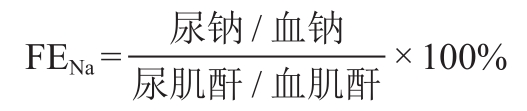
\includegraphics[width=1.75in,height=0.36458in]{./images/Image00117.jpg}

其值> 1\%者为ATN、非少尿型ATN及尿路梗阻;<
1\%者为肾前性氮质血症。应注意尿液指标检查须在输液、使用利尿剂、高渗药物前进行,否则会影响结果。

\subparagraph{影像学检查}

有助于急慢性肾衰竭的鉴别和了解ARF的病因,以B超为首选。尿路超声显像对排除尿路梗阻很有帮助。必要时CT等检查显示是否存在着与压力相关的扩张,如有足够的理由怀疑由梗阻所致,可做逆行性或下行性肾盂造影。CT血管造影、MRI或放射性核素检查对检查血管有无阻塞有帮助,但要明确诊断仍需行肾血管造影。

\subparagraph{肾活检}

在排除了肾前性及肾后性原因后,没有明确致病原因(肾缺血或肾毒素)的肾性ARF都有肾活检指征。

\subsubsection{诊断标准问题}

ARF一般是基于Scr的绝对或相对值的变化诊断。根据原发病因,肾功能急速进行性减退(表现为进行性Scr和BUN升高),结合相应临床表现和辅助检查,对ATN一般不难作出诊断。尿量多寡不能列为ARF的必备诊断条件。但一直缺乏公认的诊断标准。

2002年
,急性透析质量倡议小组(ADQI)第二次会议制定了ARF的RIFLE分级诊断标准,该标准依据Scr、GFR和尿量的变化将急性肾衰竭分为3个等级:危险(risk)、损伤(injury)和衰竭(failure),以及2个预后级别:肾功能丧失(loss)和终末期肾病(end
stage renal disease,ESRD),见表\ref{tab31-1}。

\begin{table}[htbp]
\centering
\caption{急性肾损伤/急性肾衰竭的RIFLE分级诊断标准}
\label{tab31-1}
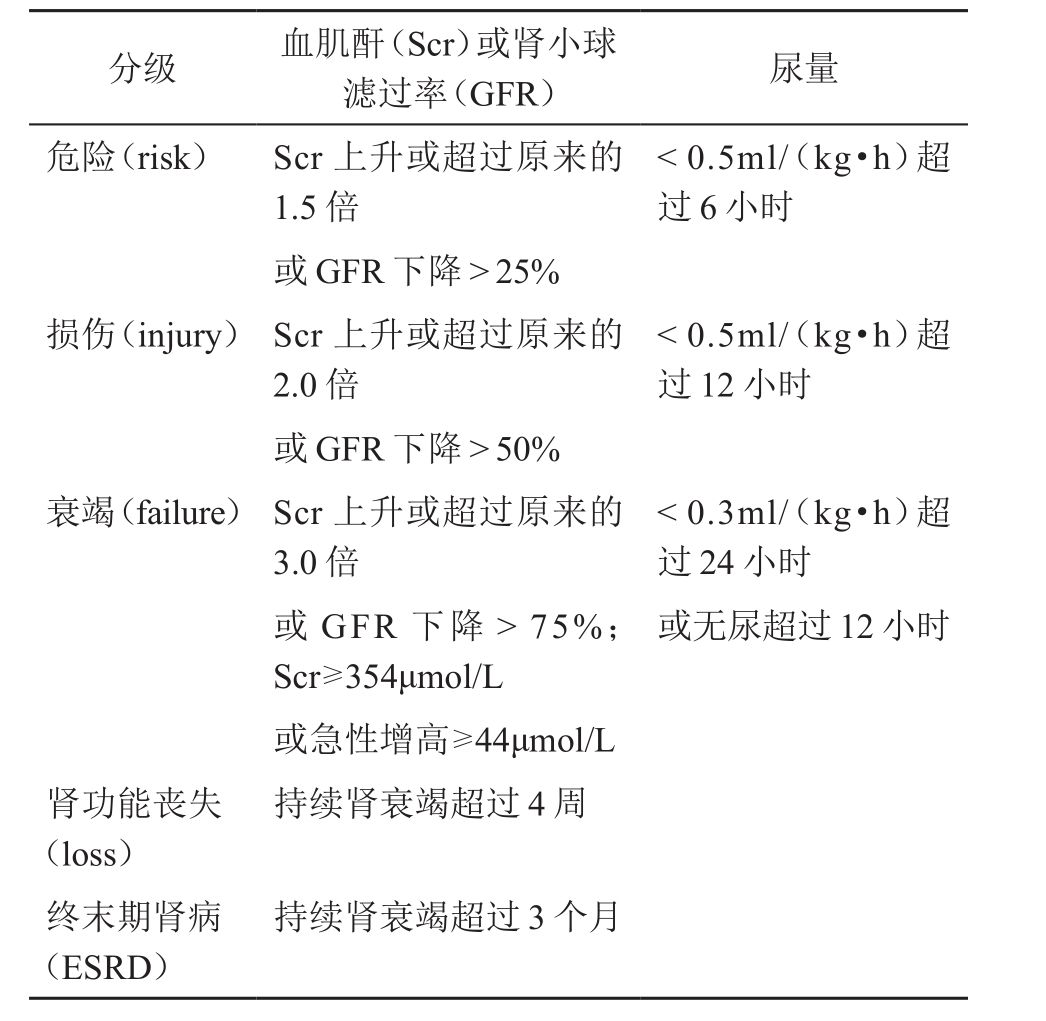
\includegraphics[width=3.47917in,height=3.39583in]{./images/Image00118.jpg}
\end{table}

2004年
,来自美国肾脏病协会(ASN)、国际肾脏病协会(ISN)、ADQI和欧洲重症医学会(ESICM)的肾脏病与急诊医学专家成立了AKIN,并在2005年9月在阿姆斯特丹举行了第一次会议,提出采用AKI替代ARF,并在RIFLE基础上对AKI的诊断及分级标准进行了修订。诊断标准为:肾功能在48小时内迅速减退,Scr升高绝对值≥26.4μmol/L,或较基础值升高≥50\%(增至1.5倍);或尿量<
0.5ml(/kg•h)超过6小时。并将AKI分为3期,分别与RIFLE标准的危险、损伤和衰竭等级相对应,见表\ref{tab31-2}。

\begin{table}[htbp]
\centering
\caption{AKIN关于急性肾损伤的分级诊断标准(基于RIFLE)}
\label{tab31-2}
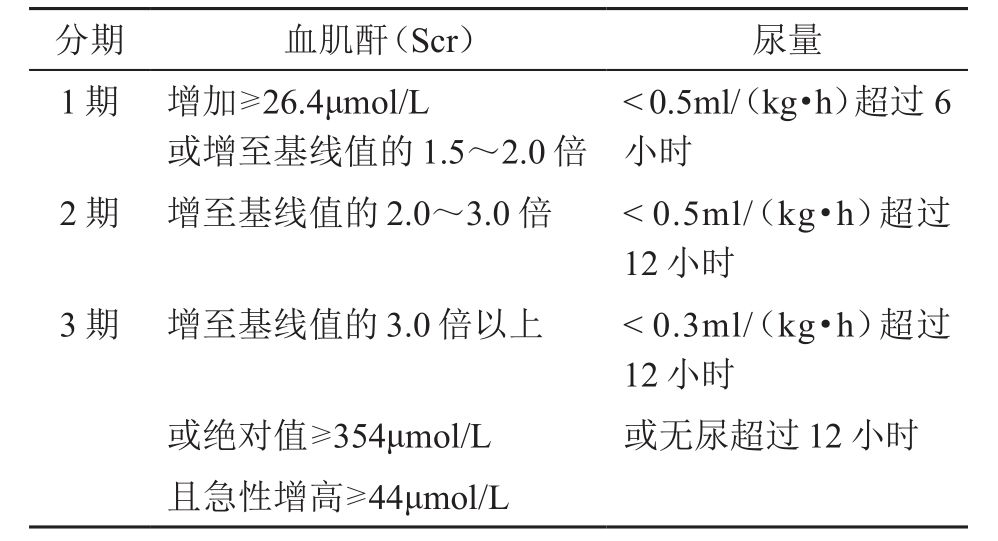
\includegraphics[width=3.32292in,height=1.79167in]{./images/Image00119.jpg}
\end{table}

该标准规定AKI的诊断时间窗为48小时,强调了Scr的动态变化,为临床早期干预提供了可行性。此外,Scr只要轻微升高就可诊断,提高了诊断的敏感性。与RIFLE标准相比,去掉了肾功能丧失和终末期肾病两个级别,因为这两个级别与AKI的严重性无关,属预后判断;去掉了GFR的标准,因为在急性状态下评价GFR困难且不可靠。但该标准是否适用于不同病因和不同临床情况下的AKI,尚需临床验证。

\subsubsection{诊断注意事项}

ARF是常见的内科急症,需按正确的诊断思路迅速做出诊断,以利治疗。首先要确定是不是ARF,其次是需鉴别是哪种ARF(肾前性、肾后性或肾性?),最后要明确导致ARF的具体病因是什么。

\hypertarget{text00083.htmlux5cux23CHP3-7-5-5-1}{}
(一) 是不是急性肾衰竭

临床上部分患者病史不清,无法判断既往有无肾脏病,就诊时已有肾衰竭,此时是ARF或慢性肾衰竭(CRF),需依下述方法来鉴别:

\subparagraph{临床资料}

①有无夜尿多病史:夜尿多是指夜间尿量超过全日尿量1/2,提示远端肾小管浓缩功能障碍,有此病史者多为CRF;②是否早期出现少尿:CRF病例到终末期(肌酐清除率<
10ml/min)才呈现少尿,因此,若肾衰竭早期即出现少尿多提示为ARF;③是否出现贫血:CRF几乎均有贫血,肾小球性及肾血管性ARF也多出现贫血,而肾小管性ARF则多无贫血或仅轻度贫血。

\subparagraph{影像学检查}

包括B超、X线平片、CT、MRI或血管造影等,而以B超为首选。ARF时肾脏常明显充血、水肿,故双肾体积常增大;而CRF时肾小球硬化、小管萎缩及间质纤维化,故双肾体积常缩小。因此,双肾体积增大者多为ARF(肾淀粉样变性或糖尿病肾病所致CRF早期,有时双肾体积亦大,应予鉴别),而双肾体积缩小者均为CRF。

\subparagraph{实验室检查}

用于鉴别ARF与CRF的实验室检查主要是指甲(头发)肌酐检查,仅在肾脏影像学检查对鉴别ARF与CRF无帮助时(即肾脏大小正常时)才应用。指甲(头发)肌酐正常而血清SCr明显增高者,提示ARF;指甲(头发)肌酐及SCr均增高者,提示CRF。

上述检查仍不能准确鉴别ARF与CRF时,可考虑进行肾活检病理检查。

\hypertarget{text00083.htmlux5cux23CHP3-7-5-5-2}{}
(二) 是哪种急性肾衰竭

ARF确诊后,则应鉴别是哪种ARF,肾前性、肾后性或肾性?因该三种ARF的治疗与预后均不相同。

\subparagraph{肾前性 ARF}

常继发于各种严重疾病引起的周围循环衰竭(休克),引起肾血流灌注不足,导致GRF减少,因而发生氮质血症。肾脏本身无器质性病变,故本病实质上是处于一种应激状态的反应,即肾尽最大的能力以保存体内钠,而维持循环血容量。但如肾血流灌注不足的情况很严重或时间较长,则可能发展至ATN,即从功能性ARF发展成器质性ARF。确定其是否已发展至ATN十分重要,因与患者的生命攸关,且在治疗上截然不同。前者要迅速补充血容量而需大量补液,以改善肾的血流灌注以避免其进一步恶化发生ATN;后者大量补液会导致患者死于急性心力衰竭。两者的鉴别方法有:

\hypertarget{text00083.htmlux5cux23CHP3-7-5-5-2-1-1}{}
(1) 补液试验:

发病前有血容量不足、体液丢失等病史,体检发现皮肤和黏膜干燥、低血压、颈静脉充盈不明显者,应首先考虑肾前性ARF。可试用输液(5\%葡萄糖液200~250ml)和注射袢利尿剂(呋塞米40~100mg),以观察输液后循环系统负荷情况。若补足血容量后血压恢复正常,尿量增加,则支持肾前性ARF的诊断。低血压时间长,尤其是老年人伴心功能欠佳时,补液后无尿量增多者应怀疑肾前性氮质血症已过渡为ATN。

\hypertarget{text00083.htmlux5cux23CHP3-7-5-5-2-1-2}{}
(2) 尿液诊断指标:

见表\ref{tab31-3}。

\begin{table}[htbp]
\centering
\caption{鉴别肾前性 ARF与ATN的尿液诊断指标}
\label{tab31-3}
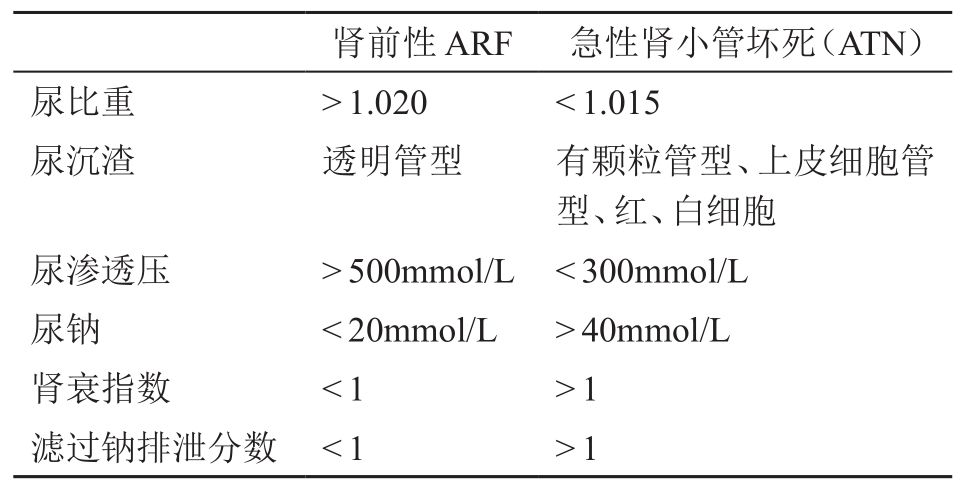
\includegraphics[width=3.26042in,height=1.63542in]{./images/Image00120.jpg}
\end{table}

\subparagraph{肾后性 ARF}

肾后性ARF是由尿路梗阻引起的肾衰竭。尿路梗阻后梗阻上方压力增高,导致肾小囊压增高,滤过压减少,从而GFR显著下降,体内代谢产物潴留。及时发现和解除梗阻可使肾功能迅速得到改善,长期梗阻则可造成不可逆性肾损害。肾后性ARF的临床特点:①有导致尿路梗阻的因素存在。尿路梗阻多由尿路器质性疾病引起(如尿路内、外肿瘤,尿路结石,血块或坏死肾组织梗阻,前列腺肥大等),也可由尿路功能性疾病导致(如神经源性膀胱)。②临床上常突然出现无尿,部分患者早期可先无尿与多尿交替,然后完全无尿,SCr及BUN迅速上升。③影像学检查常见双侧肾盂积水、双输尿管上段扩张等。若为下尿路梗阻,还可见膀胱尿潴留。尿路梗阻多数是膀胱出口梗阻,膀胱出口梗阻可用单次膀胱导尿排除之,而不需肾影像学检查;若导尿通畅,则需作肾影像学检查以明确诊断。膀胱以上的梗阻引起的ARF常为双侧性,偶亦可为单侧性梗阻,对侧肾原已有严重疾病,基本上没有肾功能,一般可用B超显像排除之。若尿路梗阻发生非常迅速(如双肾出血血块梗阻输尿管,或双肾结石碎石后碎块堵塞输尿管等),因肾小囊内压迅速增高,滤过压迅速减小,患者立即无尿,此时见不到肾盂积水及输尿管上段扩张。梗阻偶亦可发生于肾实质内,常由于某些难于溶解的物质沉积于肾小管腔内而引起肾内梗阻,如尿酸结晶(多见于肿瘤化疗后)、草酸盐结晶(某些麻醉药物引起)、钙盐结晶(甲状旁腺功能亢进、恶性肿瘤)等。

\subparagraph{肾性 ARF}

在肾前性及肾后性ARF均被排除后,肾性ARF即成立。此时需进一步鉴别是哪种肾性ARF。肾性ARF按主要病变部位可分为:肾小管性ARF(如ATN)、肾间质性ARF(如急性间质性肾炎)、肾小球性ARF(如急进性肾炎或重症急性肾炎)、肾血管性ARF(包括肾脏小血管炎,如显微镜下多血管炎及韦格纳肉芽肿病,及肾脏微血管病如溶血性尿毒症综合征等)、急性肾皮质坏死和急性肾乳头坏死引起的ARF,以前四种多见(最后两种少见)。在临床表现上,肾小管性及肾间质性ARF有很多相似处,而肾小球性与肾血管性ARF也十分相似,可将其分为两组作鉴别。两组ARF的鉴别要点:①基础肾脏病病因:ATN及急性间质性肾炎(AIN)常有明确病因,ATN常在肾缺血(如腹水、失血、休克等)或肾中毒(药物、生物毒素、重金属等中毒)后发生,AIN也常由药物过敏或感染引起,寻获这些病因,再结合临床表现,能帮助诊断;而肾小球性或肾血管性ARF多难找到明确病因。②肾衰竭发生速度:ATN
及AIN在致病因素作用后,常迅速(数小时至数日)发生肾衰竭;而肾小球性和肾血管性ARF肾衰竭发生相对较慢,常需数周时间。③肾小管功能损害:AIN常出现明显肾小管功能损害,其中肾性糖尿对提示诊断很有意义,而其他各种肾性ARF常无肾性糖尿出现。④尿蛋白排泄量:除了非类固醇抗炎药导致的AIN外(该类药物在导致AIN的同时,也能诱发肾小球微小病变病,故可出现大量蛋白尿,常>
3.5g/d),其他AIN及ATN患者尿蛋白排泄量均不多,仅轻~中度蛋白尿,罕见出现大量蛋白尿;而肾小球性和肾血管性ARF患者,尿蛋白量常较多,其中不少患者可呈现大量蛋白尿及肾病综合征。⑤急性肾炎综合征表现:ATN
和AIN患者并不呈现急性肾炎综合征,而肾小球性和肾血管性ARF患者几乎均有典型急性肾炎综合征表现。⑥确切地鉴别诊断需依赖肾穿刺病理检查。

\hypertarget{text00083.htmlux5cux23CHP3-7-5-5-3}{}
(三) 导致 ARF的病因或基础疾病是什么

在明确ARF的性质(肾前性、肾后性或肾性)后,还应力求明确其致病病因或基础疾病,这有利于制定治疗措施及判断疾病预后。如肾前性和肾后性ARF,若能明确病因并尽早去除,ARF常可自行恢复。常见的肾性ARF基础疾病的特点如下:

\subparagraph{肾小球疾病}

无论是原发性肾小球疾病(如急性肾小球肾炎、急进性肾炎、慢性肾炎急性发作),还是继发性肾小球疾病(如狼疮性肾炎、全身性坏死性血管炎、过敏性紫癜等),均可发生ARF。这些患者常在少尿的同时具有全身水肿、高血压,尿蛋白常在++~+++以上,尿检红细胞甚多,或出现红细胞管型,无严重创伤、低血压休克或中毒病史。

\subparagraph{急性间质性肾炎}

其引起的ARF,常与ATN不易鉴别,易误诊。可由药物过敏(如青霉素类、磺胺类、止痛药类等)、感染(如脓毒症、流行性出血热等)、白血病浸润肾间质及特发性等原因引起,但最常见的是药物过敏。患者可有发热、皮疹、全身淋巴结肿大、血嗜酸性粒细胞增多、血IgE增高等全身过敏表现。尿蛋白+~++,尿沉渣可仅有少量白细胞,瑞氏染色可见嗜酸性粒细胞。本病的尿指标与ATN相似,不能靠此鉴别。由于激素治疗有效,若怀疑本病,可考虑肾活检以明确诊断。

\subparagraph{急性肾血管病变}

双侧急性肾静脉血栓形成和双侧肾动脉血栓形成或栓塞均可引起ARF综合征。急性肾静脉血栓形成常发生于成人肾病综合征、肾细胞癌、肾区外伤或严重失水的肾病患儿,每同时有下腔静脉血栓形成,故常伴有下腔静脉阻塞综合征、严重腰痛和血尿。静脉肾盂造影、CT扫描和MRI有助于诊断,肾静脉造影可确诊。肾动脉栓塞可由细菌性心内膜炎等心瓣膜疾病引起,主动脉手术或造影亦可引起动脉粥样硬化斑块脱落栓塞肾动脉,肾区钝伤后也可发生。患者可完全无尿,有腰痛和腰部压痛,同时有肺、脑等脏器栓塞,常有发热和白细胞增高,可有蛋白尿和血尿,肾动脉造影可确诊。

若确实排除了上述各种可能性,表现为ARF的患者才能诊断为ATN。对诊断为ATN,但又有怀疑的患者应考虑做肾活检以明确诊断。弄清楚引起ARF的基础疾病对于患者的治疗措施选择至关重要,如确是ATN,就宜尽早透析以防止尿毒症的并发症(如感染、消化道出血等),等待肾功能自然恢复;若为药物过敏所致的急性间质性肾炎,则应永远避免使用此类致敏药物;如为狼疮性肾炎,则宜应用大剂量激素和细胞毒性药物治疗等。

\subsection{治疗}

\subsubsection{消除病因,治疗原发病}

早期干预治疗ARF首要原则是纠正和治疗致ATN的可逆病因和原发病。对于各种引起ATN的原发病(如严重外伤、严重感染等),应进行积极妥善的治疗,尤其是要处理好血容量不足、休克和清除坏死组织等。同时应停用影响肾灌注或肾毒性的药物。

\subsubsection{起始期的处理}

若能在起始期内给予恰当的处理,则ATN可逆转,或使病情减轻(如使少尿型转为非少尿型),从而改善预后。肾前性氮质血症向ATN的发展过程中,临床上可由下述指标推测其是否仍在起始期:①尿渗透压/血渗透压之比为1.1~1.4;②尿钠在20~40mmol/L之间;③蛋白尿较轻,只有少量管型。为简便起见,少尿型ARF在少尿出现后24小时内可认为是ATN的起始期。如果尿渗透压/血渗透压<
1.1,则认为ATN诊断确立,应按维持期治疗,而不宜按起始期治疗。

\subparagraph{及时纠正血容量}

补足血容量,改善微循环。①快速补液试验后1~2小时内有尿量排出,而比重在1.025以上或尿渗透压在500mmol/L以上,应继续补液,直至尿量达到40ml/h以上,尿比重降至1.015~1.020之间。②经补液后测定CVP,如仍在6cmH\textsubscript{2}
O以下,提示血容量不足,应继续补液。CVP增高至8~10cmH\textsubscript{2}
O后,减慢补液速度,如CVP不再下降,说明补液已足,应停止补液,以免导致心力衰竭及肺水肿。

\subparagraph{药物治疗}

①血管活性药:既往常用多巴胺20~40mg加入5\%葡萄糖液500ml中以15~20滴/分钟速度静滴。认为小剂量多巴胺{[}0.5~2.0μg/(kg•d){]}可扩张肾血管,增加肾血流量而增加尿量,但循证医学未能证明其在预防或治疗ARF上有效。加之小剂量多巴胺也会增加包括心律失常、心肌缺血、肠缺血(伴革兰阴性菌菌血症发生增加)等危险,故临床上已不推荐使用。②呋塞米:呋塞米可扩张血管、降低肾小血管阻力,增加肾血流量和GFR,并调节肾内血流分布,减轻肾小管和间质水肿,早期应用有预防ARF的作用。应用袢利尿剂可能会增加尿量,从而有助于清除体内过多的液体。在判断无血容量不足的因素后,用呋塞米40~100mg静注或快速静滴,若1~2小时后尿量无明显增加,可再用呋塞米80~200mg;若1~2小时后仍不增加尿量,则说明已进入ATN的维持期,不应再用。再用呋塞米可引起蓄积中毒而致耳聋和引起间质性肾炎而加重肾损害。但循证医学证实它对已发生的、需要透析的ARF患者生存率和肾功能恢复无效。

\subparagraph{其他药物}

如心房利钠肽(ANP)、一氧化氮(NO)、胰岛素样生长因子-Ⅰ(IGF-Ⅰ)、表皮生长因子(EGF)等均未证实对ARF治疗有帮助。

\subsubsection{维持期的处理}

主要是调整体液平衡,防治尿毒症综合征(如高钾血症、代谢性酸中毒等),治疗感染等。

\subparagraph{控制入液量 、维持体液平衡}

每日入液量=前一日液体出量(包括尿量、大便量、呕吐物、伤口渗出液等)+
500ml{[}500ml约等于从皮肤、呼吸排出的不显性失液量(800ml)减去代谢内生水量(约300ml)的大约数{]}。若有发热,体温每升高1℃,应增加入液量80~100ml/d。判断入液量是否恰当的参考指标为:①体重每日下降0.2~0.5kg。若体重不减轻或增加,表示入液量过多,有水、钠潴留;若每天体重下降超过1kg,则表示入液量不足或处于高分解代谢状态。②血钠保持在130~145mmol/L。若血钠<
130mmol/L而又无特殊失钠原因,则为稀释性低钠血症,表示入液量过多;若血钠>
145mmol/L,表示补液量不足。③没有水过多的表现如水肿、心力衰竭、血压升高等。④CVP不高。轻度的水过多,仅需要严格限制水的摄入。如有明显的水过多,上述措施无效,应立即进行透析治疗。

\subparagraph{饮食和营养}

ARF患者每日所需能量应为146.5kJ
(35kcal)/kg,主要由碳水化合物和脂肪供应。每日摄入蛋白质量宜在0.8g/kg以下,应选用优质动物蛋白如鸡蛋、牛奶、鱼肉或瘦肉等,因其含有较丰富的必需氨基酸(EAA)。若静脉补充EAA,可适当减少蛋白质的摄入。在EAA及足量热量供应的情况下,机体能利用体内潴留的尿素氮合成非EAA,后者再与治疗时输入的EAA一起合成体内蛋白质,从而改善患者的营养状态,减轻氮质血症,改善尿毒症症状,减少并发症和降低病死率。因此,多数学者推荐使用静脉导管滴注高营养注射液(肾衰注射液)------主要由8种必需的L-氨基酸、多种维生素及高浓度葡萄糖组成。目前,对于合并肺炎、脓毒症和消化道出血等及高代谢型的患者,均推荐使用高营养注射液,但应监测血钠、钾、CO\textsubscript{2}
CP和血糖的水平。能进食者应尽可能从胃肠道营养,给予清淡流质或半流质,以不出现腹胀和腹泻为原则。食物中的成分应尽可能地减少钠、钾含量,每日摄入两者均不宜超过20mmol。饮食中应含有较丰富的维生素,尤其是水溶性维生素如复合维生素B和C。若患者行透析治疗,则透析后每日的热量、蛋白质和食物的其他成分可不严格限制,如蛋白质可给予1g/(kg•d)。

\subparagraph{纠正代谢性酸中毒}

当CO\textsubscript{2} CP < 15mmol/L或pH
<7.2,可适当补充碱性药物。在紧急情况下,可先输入5\%碳酸氢钠液按3~5ml/kg计算(约150~250ml),以后酌情补之。对严重酸中毒者,应立即开始透析。补碱过快或过量会造成:①血钙离子化程度降低,引起手足抽搐甚至心跳突然停止;过量补碱也可引起低血钾诱发心律失常;②血pH升高,血红蛋白氧亲和力增加,组织缺氧加重;③CO\textsubscript{2}
易透入细胞内造成矛盾性酸中毒而使心肌细胞和脑细胞功能损害;④过多补碱增加血容量导致心力衰竭的发生。

\subparagraph{纠正电解质失衡}

有如下几种类型:

\hypertarget{text00083.htmlux5cux23CHP3-7-6-3-4-1}{}
(1) 高钾血症:

是ARF的重要死因之一,一般应将血钾控制在6mmol/L以下。预防措施有:①积极控制感染和酸中毒,彻底清创,防止消化道出血;②供给足够的热量;③限制钾入量(食物、药物),不输库存血;④防治血管内溶血。若血钾>
6.5mmol/L时,应紧急处理:①10\%葡萄糖酸钙液10~20ml静注(高钾心脏毒性时首选),可快速对抗高钾血症的心肌毒性作用,但维持疗效时间短。对用过洋地黄制剂的患者不宜用钙剂。②5\%碳酸氢钠液100ml静注(5分钟内),或5\%碳酸氢钠液300ml或11.2\%乳酸钠液60~100ml静滴,以提高血pH,使钾离子向细胞内移动,从而降低血钾,其作用可维持数小时,对心力衰竭者慎用。③50\%葡萄糖液50ml静注,同时皮下注射普通胰岛素8~10U;或25\%葡萄糖液300ml
+普通胰岛素15U静滴,能在促进糖原生成的过程中将钾离子转入细胞内。注射后30分钟左右即可降低血钾1~2mmol/L,维持数小时。④聚磺苯乙烯(降钾树脂):每次口服10~30g,每日1~4次,连用2~3天。可增加肠道钾排出,降低血钾。上述措施仅为临时性的应急措施,疗效仅维持2~6小时,必要时可重复应用。最有效、最彻底的措施是尽早作血液净化疗法(透析疗法),以去除体内过多的钾。

\hypertarget{text00083.htmlux5cux23CHP3-7-6-3-4-2}{}
(2) 低钙与高磷血症:

低钙血症若无症状,可不处理;伴有抽搐者,可用10\%葡萄糖酸钙液10~20ml静注。高磷应以预防为主,如供给足够热量,减少蛋白分解,避免高磷饮食,口服磷络合剂如氢氧化铝凝胶(30ml,每日3次口服)等。

\subparagraph{防治并发症}

①急性左心衰竭与肺水肿:最好治疗措施是尽早进行透析治疗,危急时用毛花苷丙(西地兰)0.4mg静注或酚妥拉明5mg静注,继以酚妥拉明10~30mg加入5\%葡萄糖液中静滴。②感染:ATN并发感染时,常不发热,白细胞也可不升高,但末梢血白细胞可出现中毒颗粒。当临床上遇到不能解释的心动过速、低血压和呼吸困难时要警惕发生感染的可能,尤应注意肺部、褥疮、静脉导管和停留尿管等部位的感染。一旦发生感染,尽可能选用对肾脏无毒性或毒性较小的抗生素治疗,其剂量应根据肾功能损害的程度而定,但应足量。③消化道出血、高血压、抽搐等处理参见有关章节。

\subparagraph{透析疗法}

明显的尿毒症综合征,包括心包炎和严重脑病、高钾血症、严重代谢性酸中毒、容量负荷过重对利尿药治疗无效者都是透析治疗指征。一般非高分解代谢的较轻的ARF患者,可试行内科保守治疗。对重症患者主张早期预防性透析治疗,即在ARF出现并发症之前即开始透析,其优点是:①对容量负荷过重者可清除体内过多的水分,以避免发生急性肺水肿或脑水肿;②清除尿毒症毒素,使毒素所致的各种病理生理变化、组织细胞损伤减轻,有利于肾损伤细胞的修复和再生;③纠正高钾血症和代谢性酸中毒,以稳定机体内环境;④有助于液体、热量、蛋白质及其他营养物质的摄入;⑤在并发症出现之前作早期预防性透析,可以使治疗简单化。因此,早期预防性透析治疗,不但可以减少心力衰竭、高钾血症、加杂感染和消化道出血等并发症的发生,而且可以缩短患者的恢复期,还能简化治疗,改善患者的一般状态,无需严格地限制饮食,是降低病死率、提高存活率的关键措施,也是本病的最佳治疗措施。紧急透析指征:①急性肺水肿,或充血性心力衰竭;②严重高钾血症,血钾>
6.5mmol/L,或心电图出现明显异位心律,伴QRS波增宽。一般透析指征:①少尿或无尿2天以上;②已出现尿毒症症状,如恶心、呕吐、神经精神症状等;③高分解代谢状态;④出现体液潴留现象;⑤血pH在7.25以下,实际重碳酸氢盐在15mmol/L以下或CO\textsubscript{2}
CP在13mmol/L以下;⑥BUN≥17.8mmol/L,除外肾外因素引起,或Scr≥442μmol/L;⑦对非少尿患者出现体液过多、球结膜水肿、心脏奔马律或CVP高于正常;⑧血钾>
6.5mmol/L,或心电图疑有高钾图形者。

\subsubsection{恢复期的处理}

最初3~5天,血肌酐、BUN可继续升高,仍按维持期治疗处理。以后须注意失水及低钾血症等的发生。液体的补入量一般为尿量的1/3~2/3即可,其中半量补充生理盐水,半量用5\%~10\%葡萄糖液。尿量超过1500~2000ml/d时应补充钾盐。应加强营养,给予高糖、高维生素、高热量饮食,并给予优质蛋白,必需氨基酸制剂等,一切营养尽可能从口摄入。同时应防治感染。

进入恢复期2~4周后,应适当锻炼,增强体质,促进机体早日恢复,定期随访肾功能,避免使用损害肾脏的药物及一切对肾脏有损害的因素(如手术、创伤)。并可试用丸药调治,如脾气虚者用香砂六君丸;肾阳虚者用金匮肾气丸;肾阴虚者用六味地黄丸,促进身体更快地恢复。一般需3~6个月即可恢复到原来的健康水平。但少数患者,由于肾脏形成不可逆损害,转为慢性肾功能衰竭。

随着透析疗法的不断改进和早期预防性透析的广泛开展,直接死于ARF本身的病例显著减少,而主要死于原发病和并发症,尤其是MODS。目前ARF的平均病死率约50\%左右。其中手术或创伤后所致的ARF,病死率约为50\%~70\%;内科疾患所致者约为30\%;产科疾患所致者最低,约为15\%。ARF的主要死亡原因有:感染(脓毒症、支气管和肺部感染)、心脏因素(心力衰竭、心律失常)、呼吸道合并症(呼吸衰竭、肺栓塞)、电解质紊乱(高钾血症)和严重的出血等。

\protect\hypertarget{text00084.html}{}{}

\hypertarget{text00084.htmlux5cux23CHP3-7-7}{}
参 考 文 献

1. 陆再英 ,钟南山.内科学.第7版.北京:人民卫生出版社,2008:543

2. 陈灏珠 ,林果为.实用内科学.第13版.北京:人民卫生出版社,2009:2173

3. 王海燕.肾衰竭.上海:上海科学技术出版社,2003:13

4. Waikar SS,Liu KD,Chertow GM. Diagnosis,Epidemiology and Outcomes
of Acute Kidney Injury. Clin J Am Soc Nephrol,2008,3:844-861

5. Bagshaw SM,George C,Bellomo R,et al. A comparison of the RIFLE and
AKIN criteria for acute kidney injury in critically ill patients.
Nephrol Dial Transplant,2008,23(5):1569-1574

6. 张文武 .急诊内科学.第2版.北京:人民卫生出版社,

2007:362

\protect\hypertarget{text00085.html}{}{}

\chapter{慢性肾衰竭}

慢性肾衰竭(chronic renal failure,CRF)指的是慢性肾脏疾病(chronic
kidney
disease,CKD)进行性进展引起肾脏结构和功能不可逆的损失,从而导致的代谢产物和毒素潴留、水电酸碱平衡紊乱以及内分泌功能紊乱为表现的临床综合征。CKD是指肾脏损伤(表现为肾脏病理学异常或血、尿液成分、影像学检查异常提示存在肾脏损伤)≥3个月,伴或不伴肾小球滤过率(GFR)的下降;或不论是否存在肾脏损伤,GRF
< 60ml/(min•1.73m\textsuperscript{2} )持续时间≥3个月。

根据1992年中华肾脏病学会全国肾小球疾病座谈会的意见,国内将CRF分为以下四个阶段:

\subparagraph{肾功能代偿期}

GFR为50~80ml/(min•1.73m\textsuperscript{2}
),血清肌酐(Scr)为133~177μmol/L(1.5~2.0mg/dl),一般无临床症状,又称肾储备功能减退期。

\subparagraph{肾功能失代偿期}

GFR为20~49ml/(min•1.73m\textsuperscript{2}
),血清肌酐为186~442μmol/L(2.1~5.0mg/dl),除轻度贫血、消化道症状、夜尿增多外无明显不适,但在劳累、感染、血压波动或进食蛋白质过多时临床症状加重,又称氮质血症期。

\subparagraph{肾功能衰竭期}

GFR为10~19ml/(min•1.73m\textsuperscript{2}
),血清肌酐为451~707μmol/L(5.1~8.0mg/dl)。大多有较明显的消化道症状及贫血症状,有轻度代谢性酸中毒及钙磷代谢异常,水电解质紊乱尚不明显。此期又称尿毒症前期。

\subparagraph{尿毒症期}

GFR < 10ml/(min•1.73m\textsuperscript{2} ),血清肌酐>
707μmol/L(8.0mg/dl)。常出现各种尿毒症症状,如明显贫血、严重恶心、呕吐以及各种神经系统并发症,甚至昏迷,明显水盐代谢和酸碱平衡紊乱。此期又称终末期肾脏病(end
stage renal disease,ESRD)。

美国肾脏病基金会K/DOQI专家组对CKD分期的建议见表\ref{tab32-1}。CKD根据GFR分为五期,其后四期与国内CRF的分期相似,CKD的分期目的在于指导一体化治疗模式的进行,即针对CKD的不同阶段而采取不同的治疗策略:①CKD1期:GFR≥90ml/(min•1.73m\textsuperscript{2}
),应侧重病因、并发症的诊断、治疗,努力延缓疾病进展,减少心血管疾病危险因素;②CKD2期:GFR为60~89ml/(min•1.73m\textsuperscript{2}
),此时应估计疾病是否会进展以及进展的速度;③CKD3期:GFR为30~59ml/(min•1.73m\textsuperscript{2}
),此期应着重对并发症进行评估和治疗;④CKD4期:GFR为15~29ml/(min•1.73m\textsuperscript{2}
),开始为肾替代治疗做准备;⑤CKD5期:GFR <
15ml/(min•1.73m\textsuperscript{2} )或透析,此时应进行肾替代治疗。

\begin{table}[htbp]
\centering
\caption{美国肾脏病基金会 K/DOQI专家组对CKD分期的建议}
\label{tab32-1}
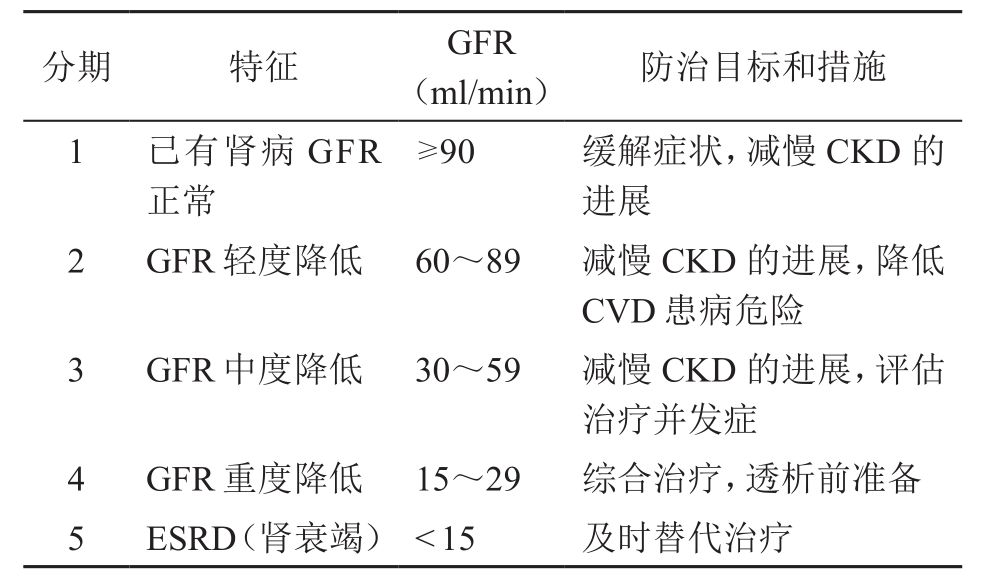
\includegraphics[width=3.33333in,height=1.92708in]{./images/Image00121.jpg}
\end{table}

CRF有时可发生急性加重或伴发ARF。如CRF本身已相对较重,或其病程加重过程未能反映ARF演变特点,则称之为“CRF急性加重(acute
progression of
CRF)”。如果CRF较轻,而ARF相对突出,且其病程发展符合ARF的演变过程,则可称为“CRF合并ARF(acute
on chronic renal failure)”其处理原则基本上与ARF相同。

\subsection{病因与发病机制}

\subsubsection{病因与危险因素}

CRF的病因可涉及肾小球病变、肾小管间质病变(慢性肾盂肾炎、慢性尿酸性肾病、梗阻性肾病、药物性肾病等)及血管病变等方面。在发达国家,糖尿病肾病、高血压肾小动脉硬化症已成为CRF的主要病因;包括中国在内的发展中国家,这两种疾病在CRF各种病因中仍位居原发性肾小球肾炎之后。根据近两年的统计资料,我国ESRD的病因中,糖尿病肾病的比例已经超过肾小球肾炎,成为导致ESRD的第一位病因。

CRF病程中急性加重的危险因素主要有:①累及肾脏的疾病(如原发性肾小球肾炎、高血压、糖尿病、缺血性肾病等)复发或加重;②血容量不足(如低血压、脱水、大出血、休克或过度利尿等);③肾脏局部血供急剧减少(如肾动脉狭窄患者应用ACEI、ARB等药物);④严重高血压未控制;⑤肾毒性药物(如氨基糖苷类药物、含碘造影剂、某些静脉用中成药物、大剂量非甾体类消炎药物);⑥泌尿道梗阻;⑦严重感染;⑧高钙血症、高尿酸血症、严重肝功能不全等。其中因血容量不足或肾脏局部血供急剧减少导致残余肾单位低灌注、低滤过状态,是导致肾功能急剧恶化的主要原因之一。在临床中,经常是多种危险因素共同存在导致的慢性肾衰竭急性加重,应仔细分析鉴别,如在积极利尿的同时使用ACEI类药物及非甾体类消炎药物,即使药物剂量不大,也可诱发肾功能衰竭的急性加重。

\subsubsection{发病机制}

慢性肾功能衰竭的发病机制曾提出尿毒症毒素学说、健存肾单位学说、肾小球高滤过学说、矫枉失衡学说、肾小管高代谢学说、脂质代谢紊乱学说等等,但没有一种能够完全解释发病的全部过程。近年来随着分子生物学的研究进展,新的学说不断涌现,如某些细胞因子、生长因子和血管活性物质对CRF的影响,加深了对慢性肾衰竭发病机制的认识。

\hypertarget{text00085.htmlux5cux23CHP3-8-5-2-1}{}
(一) 健存肾单位学说

各种原因引起的肾实质疾病
,导致大部分肾单位破坏,残余的小部分肾单位轻度受损,功能仍属正常,这些残余的“健存”肾单位为了代偿,必须加倍工作以维持机体正常的需要。从而导致“健存”肾单位发生代偿性肥大,肾小球滤过功能和肾小管处理滤液的功能增强,最终导致肾小球硬化而丧失功能,出现肾衰竭的临床表现。

\hypertarget{text00085.htmlux5cux23CHP3-8-5-2-2}{}
(二) 矫枉失衡学说

矫枉失衡学说是对健存肾单位学说的进一步发展。肾功能不全时机体内环境存在一系列不平衡的病态现象,为了矫正它,机体要作相应调整,特别是引起某些物质增加(矫枉,也称平衡适应),这些代偿改变却又导致新的不平衡,即失衡,并由此产生一系列临床症状。周而复始,造成了进行性损害。典型的例子是磷的代谢改变(如图\ref{fig32-1})。肾小球滤过率下降后,尿磷排出减少,血磷升高,血钙下降,机体为矫正这种不平衡,增加甲状旁腺激素(PTH)的分泌,促使肾排磷增多和血钙增高,使血磷血钙水平恢复正常;但随着GFR进一步下降,为维持血钙磷水平,势必不断增加PTH水平,导致继发性甲状旁腺功能亢进,引起肾性骨病、周围神经病变、皮肤瘙痒和转移性钙化等一系列失衡症状。

\hypertarget{text00085.htmlux5cux23CHP3-8-5-2-3}{}
(三) 肾小球损伤的“三高”学说

肾单位微穿刺研究表明,慢性肾衰竭时,“健存”肾单位的入球小动脉阻力下降,而出球小动脉阻力增加,导致肾小球内高压力、高灌注和高滤过。肾小球高压使小动脉壁增厚和毛细血管壁张力增高,引起缺血和内皮细胞损害,系膜细胞和基质增生,促使残余肾小球代偿性肥大,肾小球硬化,使肾功能进一步恶化。实验表明,慢性肾衰竭时,残余肾单位肾小球的高灌注、高滤过、高压力会导致肾小球毛细血管张力增加,牵拉系膜细胞,促使系膜细胞过表达胶原Ⅰ、Ⅱ、Ⅳ、Ⅴ、纤维连接蛋白和层粘连蛋白,导致系膜基质明显扩张,肾小球上皮细胞足突融合以及从肾小球基底膜上脱落,最终引起进行性肾小球硬化。晚近认为肾小球“三高”机制是促使肾小球进行性损害的关键环节之一。

\hypertarget{text00085.htmlux5cux23CHP3-8-5-2-4}{}
(四) 肾间质-小管损伤学说

肾组织学研究表明,慢性肾脏疾病患者的肾功能损害程度与慢性肾小管-间质的病理变化关系密切。残存肾单位的肾小管,尤其是近端肾小管,在慢性肾衰竭时发生代谢亢进,细胞内钙离子超载,诱导自由基的过度表达,诱发氧化应激反应,进而导致肾小管和间质细胞的炎症与纤维化,加速健存肾单位的丢失。

慢性肾病常常合并不同程度的小管间质炎症反应,而间质中浸润的淋巴-单核细胞可以释放多种不同的细胞因子和生长因子,刺激成纤维细胞的增生,加快了纤维化的进程。肾小管-间质的纤维化均伴有肾小管的萎缩,因此,肾小管-间质的纤维化是慢性肾功能衰竭的主要机制之一。

\hypertarget{text00085.htmlux5cux23CHP3-8-5-2-5}{}
(五) 脂质代谢紊乱学说

继发性高脂血症是慢性肾病的常见并发症之一
。甘油三酯和低密度脂蛋白增多,特别是富含ApoB的脂蛋白增多,而高密度脂蛋白和不饱和脂肪酸降低。肾小球上皮细胞、内皮细胞和系膜细胞表面都有脂蛋白受体,脂质可通过受体结合在肾小球内并沉积,使系膜细胞增殖基质增多;由于内皮细胞损伤,毛细血管壁巨噬细胞浸润并形成泡沫样细胞(其胞浆内含大量胆固醇和磷脂);导致肾小球硬化,加速肾功能的损害。

\begin{figure}[!htbp]
 \centering
 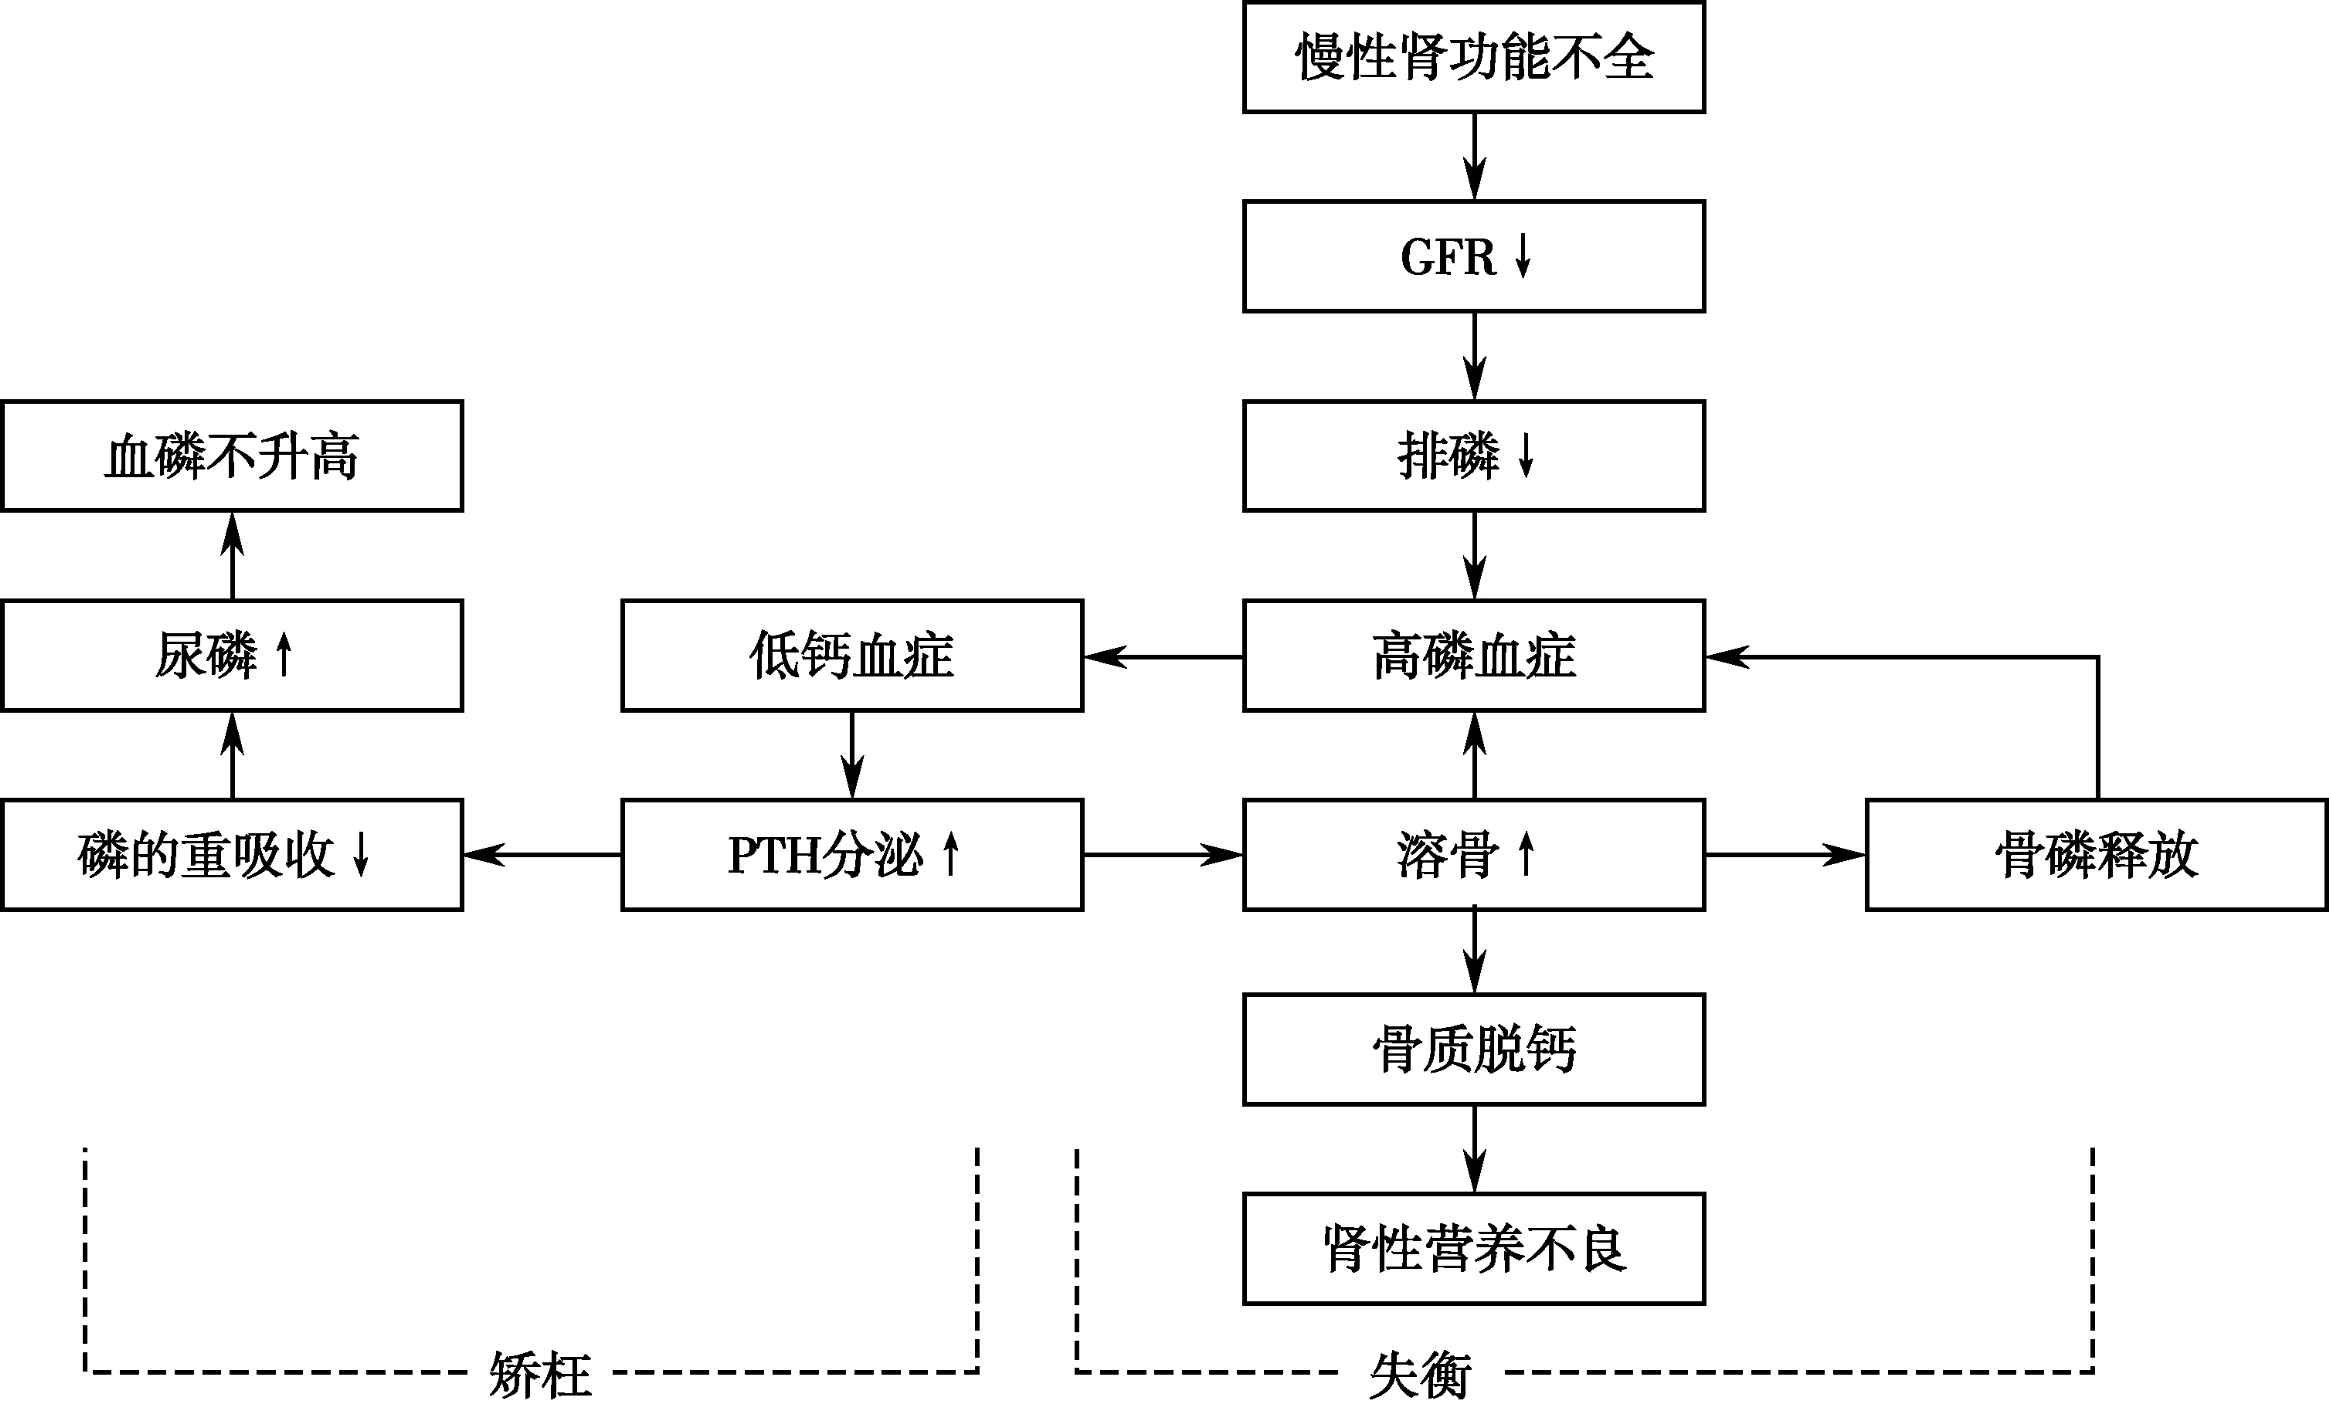
\includegraphics[width=5.02083in,height=3.03125in]{./images/Image00122.jpg}
 \captionsetup{justification=centering}
 \caption{矫枉失衡学说示意图}
 \label{fig32-1}
  \end{figure} 

\hypertarget{text00085.htmlux5cux23CHP3-8-5-2-6}{}
(六) 钙磷沉积和继发性甲旁亢

在 CRF时,1,25(OH)\textsubscript{2} D\textsubscript{3}
的缺乏、低钙血症、高磷血症等因素,致继发性甲旁亢的发生和发展,是引起肾单位损害加重的另一因素。过多的甲状旁腺激素(PTH)可引起软组织转移性钙化,致肾小管上皮细胞内钙沉着增多,引起肾小管-间质钙化的发生和发展,致肾单位损害不断进展。

\hypertarget{text00085.htmlux5cux23CHP3-8-5-2-7}{}
(七) 细胞因子和生长因子的重要作用

近年发现,在CRF病程进展过程中,有不少细胞因子或生长因子参与了其病理生理过程。按其作用可分为四类:①前炎症因子:补体激活物(C3a、C5a),白介素(IL-1、IL-2、IL-6)、TNFα;②血管活性物质:血栓素、前列腺素、血管紧张素;③生长因子和基质诱生因子:转化生长因子(TGFβ)、成纤维细胞生长因子(FGF)、胰岛素样生长因子(IGF-1)、血小板源生长因子(PDGF)等;④细胞外基质与蛋白酶:Ⅳ胶原、核心蛋白聚糖。这些因子或者与肾小球系膜增殖、肾小管肥大有关,或者与间质的细胞浸润有关,或者与微血管内凝血有关,进一步促进肾脏病的进展。

\hypertarget{text00085.htmlux5cux23CHP3-8-5-2-8}{}
(八) 蛋白尿学说

近年来,人们观察到尿蛋白在肾小管和间质损害中的作用,临床与实验均证实蛋白尿不仅是肾实质受损的重要临床表现,而且还是直接肾脏损伤的独立因素。对于慢性肾病患者而言,无论是否存在高血压,ACEI均可明显降低尿蛋白,延缓肾功能下降的趋势。在出现大量尿蛋白的患者,肾小球内常有大量脂蛋白积聚,脂质的过氧化可以引起肾功能的损伤;当尿蛋白超过近端小管的吸收能力时,肾小管上皮细胞胞饮原尿中过多的蛋白质,则可诱发细胞内溶酶体的破裂,溶酶体蛋白酶的释放反过来导致近端肾小管上皮的损伤,加重肾脏的损害。

\hypertarget{text00085.htmlux5cux23CHP3-8-5-2-9}{}
(九) 肾内缺氧学说

肾内血流动力学的紊乱引起肾小球缺氧。系统性高血压和肾小球内的高压均可引起肾小球及其周围血管内皮损伤,增生性肾脏病还会引起肾小球的毛细血管丛堵塞,引起和(或)加重肾内缺氧,而缺氧又可导致各种炎症介质和生长因子的产生增加,加重肾脏病的进展。

\hypertarget{text00085.htmlux5cux23CHP3-8-5-2-10}{}
(十) 尿毒症毒素学说

目前,已经发现尿毒症患者体内至少存在200种以上的尿毒症毒素,其中部分尿毒症毒素对肾组织具有损害作用(如甲基胍、PTH等)。例如,将CRF动物体内甲基胍浓度降低以后,其血肌酐水平上升速度减慢,肌酐清除率下降减慢,提示甲基胍可能具有促进肾功能恶化的作用。可见这些毒素与尿毒症代谢紊乱或临床表现密切相关。

\subsection{诊断}

\subsubsection{临床表现特点}

\subparagraph{水、电解质代谢紊乱和酸碱平衡失调}

以代谢性酸中毒和水钠平衡紊乱最常见。

\hypertarget{text00085.htmlux5cux23CHP3-8-6-1-1-1}{}
(1) 代谢性酸中毒:

在部分轻、中度CRF(GFR > 25ml/ min,或Scr <
350μmol/L)的患者中,由于肾小管泌氢功能受损或近端肾小管重吸收碳酸氢盐的能力下降,因而发生阴离子间隙正常的高氯血症性酸中毒,即肾小管性酸中毒;当GFR
< 25ml/min(或Scr >
350μmol/L)时,机体的代谢产物,如磷酸、硫酸等酸性物质因肾脏的排泄功能障碍而潴留于体内,可发生阴离子间隙升高的高氯血症性酸中毒,即所谓的“尿毒症性酸中毒”。

\hypertarget{text00085.htmlux5cux23CHP3-8-6-1-1-2}{}
(2) 水钠代谢紊乱:

主要表现为水钠潴留,有时也可表现为低血容量和低钠血症。

CRF时,肾脏调节钠平衡的能力虽有所下降,但患者血钠水平仍能在较长时间内保持在正常范围。这主要是由于进行性肾衰患者GFR和肾小管重吸收功能均有下降,两者在慢性肾衰的早期建立了一种暂时的平衡。即由于肾小球滤过面积的减少,滤过钠总量亦因之而减少,但肾小管重吸收钠也相应减少,故每日尿钠排泄量仍可不变。但这种平衡有一定限度,随着CRF的进展,有效肾单位的丧失,肾贮钠能力可受到损害。

由于有效肾单位的丧失,肾脏贮钠的能力受损。如果钠的摄入不足就会导致体内钠的缺乏。临床上常见的低钠原因有:①肾小管重吸收钠减少;②渗透性利尿,使钠丢失增加;③长期恶心、呕吐、腹泻等的丢失;④限制钠盐摄入;⑤使用强利尿剂等均可造成低钠血症。低钠血症时患者不能及时减少尿钠,致使细胞外液量的减少,有效循环血容量不足,肾血流量降低,进一步促使肾小球滤过率的下降,肾功能恶化,从而使早期CRF患者出现明显的尿毒症症状,并伴低血容量的表现:头晕、乏力、直立性低血压、肌痉挛、抽搐,严重时可有低血压、休克、昏迷。

慢性肾衰时高钠血症亦较常见。常因肾脏失去体内钠盐的调节能力,此时CRF患者如摄入过多的钠,极易导致钠潴留,严重时可因水肿和高血压而诱发心力衰竭。

\hypertarget{text00085.htmlux5cux23CHP3-8-6-1-1-3}{}
(3) 钾代谢紊乱:

高钾血症和低钾血症均可见,以高钾血症更多见。

CRF早期,血钾常能维持在正常水平,一般不出现高钾血症。这主要是由于:①局部肾素血管紧张素系统活化,刺激醛固酮的分泌,肾远端小管在醛固酮作用下,增加了钾的排泄;②地高辛样物质可以抑制钠泵的活动,促进钾的排泄;③残余肾单位中,滤过液钠浓度偏高,有利于集合管中钾的排泄;④代谢性酸中毒;⑤肾小管重吸收碳酸氢盐能力不足,到达集合管的碳酸氢盐促进了钾分泌;⑥局部多巴胺样作用加强。

随着肾衰的进展,当GFR降至20ml/min或更低时,肾调节钾代谢的能力明显降低。此时即使钾的摄入正常,患者仍然容易出现高钾血症。主要由于:①少尿;②损伤的肾单位细胞内钾外溢;③肾脏失去排酸能力,出现代谢性酸中毒,细胞外氢离子进入细胞内,与钾交换,导致血钾升高;④分解代谢增加(感染、手术等)、输库存血、摄入富含钾的食物和使用影响血钾的药物等。

大部分高钾血症患者无自觉症状,直至发生心律失常或心跳骤停时,通过心电图和(或)测血清钾时才发现。临床上常出现心肌抑制表现,如心音低钝,心率缓慢,心律失常甚至心跳骤停;也常见骨骼肌症状,如肢体麻木、乏力、无力及麻痹、瘫痪,症状常由下肢向上发展;可出现昏厥和神志障碍;有时可以出现呼吸肌抑制,导致呼吸停止。

低钾血症的发生包括两个方面,一方面由于体内水的潴留出现稀释性低钾,此时有低钾表现,而机体总钾含量并不少,主要是体内钾的重新分布所致;另一方面由于摄入过少,加上呕吐、腹泻、利尿的丢失,造成了体内总体钾的缺乏,出现真正的低血钾。低血钾的临床表现是消化道麻痹症状,如腹胀、肠鸣音减弱;心脏表现为心律失常,如期前收缩、阵发性心动过速等;骨骼肌症状,如肌无力和肌麻痹等,以四肢肌肉的表现最突出。

\hypertarget{text00085.htmlux5cux23CHP3-8-6-1-1-4}{}
(4) 钙磷代谢紊乱:

主要表现为低钙血症和高磷血症,少部分慢性肾衰竭患者由于甲状旁腺增生,持续释放甲状旁腺激素,出现高钙血症,偶尔产生骨痛和转移性钙化,当转移性钙化累及心脏传导系统时可导致猝死。

\hypertarget{text00085.htmlux5cux23CHP3-8-6-1-1-5}{}
(5) 镁代谢紊乱:

慢性肾衰竭时常有高镁血症,其程度常与GFR下降程度平行。

\subparagraph{蛋白质}

、糖类、脂肪和维生素代谢紊乱
①蛋白质代谢紊乱:一般表现为蛋白质代谢产物蓄积,产生氮质血症;也可出现血清白蛋白降低、血浆与组织必需氨基酸水平下降等;②糖代谢紊乱:主要表现为糖耐量降低和低血糖症,以前者多见;③脂肪代谢紊乱:高脂血症相当常见;④维生素代谢紊乱:经常出现,如血清维生素A水平增高、维生素B\textsubscript{6}
及叶酸缺乏等。

\subparagraph{心血管系统表现}

心血管病变是CKD患者的主要并发症之一,也是CKD患者最常见的死因。慢性肾衰竭患者心血管系统异常主要表现为动脉粥样硬化、高血压、心力衰竭、尿毒症性心肌病、尿毒症性心包炎、左心室肥厚、冠状动脉疾病等。有研究显示,尿毒症(CKD5期)患者心血管不良事件及动脉粥样硬化性心血管病发生率比普通人群高15~20倍。而心力衰竭更是尿毒症患者最常见的死亡原因。

\subparagraph{消化系统表现}

消化道症状虽然不具备特异性,但这些症状是慢性肾衰竭患者最早和最突出的表现,常可成为慢性肾衰竭的诊断线索。在众多的消化道症状中,食欲减退是最早出现的临床表现,随着病情的加重,进而出现恶心、呕吐、腹泻、口腔有尿味等表现。消化道出血也是常见表现。

\subparagraph{呼吸系统表现}

慢性肾衰竭患者可以出现肺活量减低、限制性通气功能障碍和(或)弥散功能障碍。在终末期(CKD5期),还可以出现尿毒症肺水肿、尿毒症性胸膜炎及肺钙化表现。

\subparagraph{血液系统表现}

慢性肾衰竭患者血液系统异常主要表现为肾性贫血和出血倾向。贫血多表现为低增殖性的,正细胞正色素性贫血,外周血网织红细胞计数减少。轻度出血倾向表现为皮下瘀斑、紫癜、鼻出血、牙龈出血或结膜出血,严重时可出现出血性心包炎、消化道及颅内出血,危及患者生命。

\subparagraph{神经肌肉系统表现}

①尿毒症脑病:临床上常为非特异性表现,早期表现为淡漠、乏力、记忆力减退、失眠、易激惹等。随着病情的加重,可出现定向力及计算力障碍、情绪低落、精神错乱。晚期可出现扑翼样震颤、多灶性肌痉挛、手足抽搐、癫痫或昏迷;②尿毒症性周围神经病变:早期主要侵犯感觉神经,表现为下肢远端感觉异常,如肢体麻木,有时有蚁走感、烧灼感等,后期侵犯运动神经,出现下肢不自主运动(常表现为下肢的抽动或摆动)时,也称为“不安腿”或“灼足”综合征,多发生在晚上,活动后可缓解;晚期有膝反射和跟腱反射的丧失。脑神经损伤也可见,如瞳孔不对称、面瘫、展神经麻痹、听力障碍等;③尿毒症肌病:尿毒症肌肉系统的病变常表现为易疲劳、肌无力和肌萎缩,严重者出现工作和活动能力受限,体检时可发现肌力减退,尤其是下肢近端肌力较上肢肌力减弱出现得更早,程度也更严重。

\subsubsection{实验室检查}

在急诊工作中,判断患者是否患有慢性肾衰竭,肾衰竭的程度如何,不仅要根据病史、症状和体征,而且要及时了解反映肾功能的各项实验室检查或影像学检查。慢性肾衰竭是一种多系统器官损害的综合征,因此对各系统的检查都应及早进行。

\subparagraph{肾功能检查}

目前常用的肾功能指标是血清肌酐(Scr)和内生肌酐清除率(Ccr),并且以血尿素氮(BUN)水平作为肾功能的参考指标。目前认为,男性Scr
< 106.1μmol/L (1.2mg/dl),女性Scr <
88μmol/L(1.0mg/dl)为正常;如果Scr > 133μmol/L(1.5mg/dl)或Ccr <
80ml/min认为肾功能减退;如果BUN >
7.14mmol/L(20mg/dl)时,应考虑肾功能受损的可能性,但应除外高蛋白饮食、脱水、低血容量、感染、肠道内出血以及服用某些药物的影响,如呋塞米、四环素等。近些年应用核医学测定肾小球滤过率反映肾小球滤过功能,其准确性比肌酐清除率要高。

肾图检查一般可以初步了解慢性肾功能损害的情况,并对急慢性肾衰的鉴别诊断有意义。如果肾图血管段、分泌段和排泄段均很差,则提示慢性肾衰竭可能性大。

\subparagraph{电解质测定和血气分析}

慢性肾功能衰竭患者常出现代谢性酸中毒、电解质紊乱,因此慢性肾衰竭患者需要急诊做电解质检查,应及时做血气分析或测定二氧化碳结合力检查以明确有无代谢性酸中毒、电解质紊乱。

\subparagraph{肾小管功能检查}

慢性肾衰竭患者尿浓缩功能降低表现为尿渗透压、尿比重降低。如果患者肾小球滤过率轻度下降,但出现明显的代谢性酸中毒,如此时患者没有腹泻、脱水等情况,则此种酸中毒多为肾小管酸中毒。进一步检查需要做血气分析、尿气分析、尿渗透压、尿氨基酸、尿酸化实验室检查。

\subparagraph{尿液分析}

对于慢性肾衰竭患者来说,尿液分析对慢性肾衰竭的病因诊断有重要意义。因此对尿液中的蛋白、红细胞、白细胞、管型、葡萄糖等项目的检查应重视。对于晚期慢性肾功能衰竭患者,尿液分析的诊断意义相当有限。因此对尿液分析结果无明显异常的慢性肾功能衰竭患者切不可简单认为肾脏正常。

\subparagraph{营养状态}

营养状态是决定慢性肾功能衰竭患者并发症发生率和存活率的重要因素之一。血清白蛋白、前白蛋白、转铁蛋白、PCR是检测和评价慢性肾功能衰竭患者营养状态的常用指标。

\subparagraph{贫血和出血倾向的检查}

慢性肾功能衰竭患者肾性贫血发生率高,并且铁的缺乏也相当常见。因此,需要定期检测血清铁浓度、总铁结合率、转铁蛋白等的水平,以了解贫血、缺铁及缺铁的程度。但血清铁<
90μg/dl,铁蛋白< 100μg/dl时,一般需要补充铁剂。当血红蛋白<
60g/L时可以考虑输血治疗。

\subparagraph{关于肾性骨病的检查}

与肾性骨病相关的检查,包括血生化、尿生化、骨密度、骨活检。其中骨活检准确率高,是诊断肾性骨病的金标准。血生化包括碱性磷酸酶、甲状旁腺激素(PTH)、骨钙素(BGP)等。

\subparagraph{影像学检查}

应用B超、X线、CT、核医学等方法可以了解肾脏和泌尿系统的形态、大小、功能等情况,有助于慢性肾功能衰竭的诊断和鉴别诊断。如上述检查发现双肾缩小,则支持慢性肾功能衰竭的诊断;胸部影像检查有助于发现患者心脏扩大、心包积液、肺水肿、肺部感染等情况。核医学有助于骨病和肾脏形态及功能的明确。

\subparagraph{其他相关检查}

心电图、脑电图、肌电图、骨密度、感染患者病原体的检查。

\subparagraph{慢性肾功能衰竭时急诊应进行的检查项目}

①病史采集;②密切观察尿毒症症状;③生命体征监测,记录24小时出入量;④尿量、比重、尿常规;⑤肾功能(血肌酐、尿素氮);⑥血、尿渗透压;⑦电解质;⑧血气分析;⑨贫血与出凝血时间;⑩心电图和胸部X片等。

\subsubsection{诊断注意事项}

\subparagraph{慢性肾衰竭诊断的主要内容}

对慢性肾衰竭患者进行诊断时,其主要内容包括:①慢性肾衰竭的确立与分期;②病因诊断(如慢性肾小球肾炎、糖尿病肾病、高血压性肾脏损害);③并发症的诊断(如肾性贫血、肾性骨病、感染、出血);④是否存在加重肾功能恶化的急性可逆因素。

\hypertarget{text00085.htmlux5cux23CHP3-8-6-3-1-1}{}
(1) 原发病诊断:

早期慢性肾衰的原发病可通过肾活检等检查得到诊断,到晚期则比较困难。但如能确诊梗阻性肾病、慢性肾盂肾炎、肾结核、糖尿病肾病、痛风性肾病、系统性红斑狼疮等仍有治疗价值。对病因尚不明者先积极治疗尿毒症,待病情改善后再进一步检查。

\hypertarget{text00085.htmlux5cux23CHP3-8-6-3-1-2}{}
(2) 尽量检出加重慢性肾衰的可逆因素:

①有效血容量不足:常见于钠水丢失、出血等,可使GFR下降,加重肾衰。②感染:常见者有呼吸道、泌尿系和皮肤感染,包括一些隐匿性感染。③尿路梗阻:最常见者为尿路结石,包括完全性或不完全性梗阻。④肾毒性药物:最常见者为氨基苷类抗生素和造影剂的使用。⑤严重心血管病变:包括严重高血压、充血性心力衰竭、严重心律失常和心包填塞等。⑥急性应激状态:如严重创伤、大手术后。⑦高钙血症、高磷血症或转移性钙化。⑧高蛋白饮食等。

\subparagraph{急诊针对慢性肾衰竭患者的诊治思路}

急诊工作中,临床医师应在认真分析患者病史、症状、体征和实验室检查结果的基础上,按以下步骤进行诊治:①尽快明确是否存在严重高血压、心衰、严重酸中毒、严重高钾血症、严重出血等可能危及患者生命的急性并发症,并给予相应的对症处理;②在病情允许的情况下,根据是否存在长期肾功能不全的病史、B超是否存在肾脏萎缩、是否存在贫血等指标判断是否为慢性肾衰竭;③明确是否为慢性肾衰竭急性加重或合并有急性肾衰竭,找出导致肾功能急性加重的诱因并积极予以纠正;④尽可能明确慢性肾衰竭的病因诊断。

\subparagraph{慢性肾衰竭的鉴别诊断}

①肾前性氮质血症:肾前性氮质血症在病程的早期常表现出血清尿素氮和肌酐的不平行上升,同时伴有尿比重的升高。在有效循环血量补足48~72小时后肾前性氮质血症患者的血清肌酐、尿素氮水平会恢复正常,而慢性肾衰竭患者的肾功能则很难恢复。②急性肾衰竭:根据肾衰竭病史的长短、影像学检查结构(如B超、CT等)、贫血情况、指甲肌酐水平、甲状旁腺激素水平等指标可以做出正确的判断。

对于急诊医师而言,在诊断处理慢性肾衰竭患者的过程中,重点要注意以下几个方面的临床评估:①患者的容量状态,是否存在容量依赖性心衰;②患者的血压状况,是否存在严重高血压导致的心衰(非容量依赖性心衰)及其导致的其他心脑损伤;③重度贫血;④重度酸中毒;⑤严重的高钾血症或低钾血症。因为这些慢性肾衰竭的临床并发症,有可能危及患者的生命安全,对于急诊医师更应予以特别的关注。

\subsection{治疗}

对于慢性肾衰竭患者,不仅病情较严重的需要制定治疗计划,而且早中期症状较轻的也应该采取积极措施,控制各种临床症状,提高生活质量;又要延缓慢性肾衰竭的发展,防治肾功能损害进行性加重。早中期慢性肾衰竭主要应用非透析疗法,晚期尿毒症阶段需要依靠代替疗法,如透析和肾移植。

\subsubsection{慢性肾衰竭的防治对策和基本措施(非替代治疗)}

首先要提高对慢性肾衰竭的警觉,努力做到早期诊断。同时,对已有的肾脏疾患或可能引起肾损害的疾病(如糖尿病、高血压等)进行及时有效的治疗,防止慢性肾衰竭的发生,这就是所谓的初级预防。对于轻、中度慢性肾衰竭及时进行治疗,延缓、停止或逆转慢性肾衰竭的进展,防止尿毒症的发生。其基本对策是:①坚持病因治疗;②避免或消除慢性肾衰竭急性加重的危险因素;③阻断或抑制肾单位渐进性发展的各种途径,保护残余肾单位。在减慢肾功能衰竭的进展的同时,积极防治慢性肾衰竭的各种并发症也是治疗的重要组成部分。慢性肾衰竭非替代治疗的具体措施与目标如下,其中1~6条以减慢肾功能不全的进展为主要治疗目的,7~13条主要目的是防治慢性肾衰竭的常见并发症。

\subparagraph{控制高血压}

高血压既是慢性肾衰竭的并发症,同时也是慢性肾衰竭加重的促进因素,同时还会导致出现各种危及患者生命的心脑血管并发症,所以控制血压在慢性肾衰竭患者中尤为重要。透析前慢性肾衰竭患者血压应当控制在120~130/75~80mmHg以下,但维持透析的患者一般不超过140/90mmHg即可。常用药物有ACEI、ARB、钙离子拮抗剂、β受体阻滞剂、利尿剂,必要时还可以使用α受体阻滞剂。

\subparagraph{发挥 ACEI和ARB的独特作用}

ACEI和ARB除了具有良好的降压作用外,还有独立于降压作用之外的减低肾小球高滤过、减轻蛋白尿的作用,同时也有抗氧化、减轻肾小球基底膜损害等作用。但应注意,它们有使血钾升高及一过性血肌酐升高的作用。常用的ACEI有依那普利(10~20mg,每日2次)、贝那普利(10~20mg,每日1次)、福辛普利(10~20mg,每日1次)、卡托普利(12.5~25mg,每日2~3次)等。ARB类常用氯沙坦(50~100mg,每日1次)、缬沙坦(80~160mg,每日1次)、厄贝沙坦(150~300mg,每日1次)、替米沙坦(80~160mg,每日1次)等。

\subparagraph{控制血糖}

糖尿病患者空腹血糖应控制在5.0~7.2mmol/L(睡前6.1~8.3mmol/L),糖化血红蛋白应小于7\%。在GFR
>
60ml/min时,可还可以选用格列喹酮(糖适平,30~180mg/d)、格列苯脲(优降糖,2.5~15mg/d)、格列美脲(亚莫利,1~6mg/d)和格列齐特(达美康,40~240mg/d)。GFR
< 30ml/min时,应改用胰岛素治疗。

\subparagraph{控制蛋白尿}

将患者蛋白尿控制在小于0.5g/24小时,或明显减少微量白蛋白尿,均可改善慢性肾衰竭患者的长期预后。

\subparagraph{饮食治疗}

单独采用低蛋白、低磷饮食,或同时加用必需氨基酸及其α酮酸(EAA/αKA),可能减轻残余肾小球硬化和肾间质纤维化的作用。慢性肾衰竭患者蛋白摄入量一般为0.6~0.8g/(kg•d),磷摄入量一般应<
600~800mg/d。患者饮食中动物蛋白与植物蛋白比例一般为各占一半左右,对蛋白质摄入量限制较严的患者{[}所谓极低蛋白饮食,蛋白摄入量为0.4~0.6g/(kg•d){]},动物蛋白比例可占50\%~60\%,以增加必需氨基酸的摄入。有条件时,在低蛋白饮食的基础上,加用适量必需氨基酸及其α酮酸{[}0.1~0.2g/(kg•d){]},能更有效地减慢肾功能不全的进展,此时患者饮食中动物蛋白与植物蛋白的比例可以不加限制。此外,在限制蛋白摄入的同时,需要摄入足够的热量,一般为125.6~146.5kJ(30~35kcal)/(kg•d)。

\subparagraph{高脂血症的治疗}

透析前慢性肾衰竭患者与一般高脂血症患者的治疗原则相同,但对于维持透析的患者,高脂血症的标准应放宽,将血胆固醇控制在6.5~7.8mmol/L,甘油三酯1.7~2.3mmol/L为宜。常用他汀类降脂药,如辛伐他汀(5~40mg/d)、洛伐他汀(10~80mg/d)、普伐他汀(10~40mg/d)等。

\subparagraph{纠正贫血}

当肾性贫血导致Hb < 100~110g/L或Hct <
0.3~0.33时,即可开始使用重组人红细胞生成素(rHuEPO)治疗。开始用量为80~120IU/(kg•周),分2~3次皮下注射或静脉注射。直至Hb上升到110(女性)~120(男性)g/L时为达标。如Hb
>
130g/L,应谨慎观察并适当减量。应每个月检测血红蛋白水平,以此调整EPO剂量。个别透析患者用量可增加到200IU/(kg•周)。在使用EPO治疗的同时,应重视造血原料(铁、叶酸等)的补充,口服铁剂主要有琥珀酸亚铁(速力菲,0.1~0.2g/次,每天3次)、硫酸亚铁(0.3g/次,每天3次)等;静脉补铁以氢氧化铁蔗糖复合物(蔗糖铁)在安全性及有效性上都表现很好。慢性肾衰竭患者如Hb
< 60g/L,且有明显贫血症状时,可以少量输注红细胞悬液。

\subparagraph{口服吸附疗法和导泻疗法}

口服氧化淀粉或活性炭制剂、口服大黄制剂或甘露醇(导泻疗法)等,都是通过胃肠道增加尿毒症毒素的排出。此种疗法主要用于透析前慢性肾衰竭患者的治疗,对减轻氮质血症有一定辅助作用。

\subparagraph{防止感染}

感染是慢性肾衰竭患者常见的并发症,出现时可以导致慢性肾衰竭及其并发症的急性加重,应给予积极治疗,但在治疗中应注意尽可能选用肾毒性最小的抗生素。

\subparagraph{纠正代谢性酸中毒}

轻度酸中毒,可口服碳酸氢钠片1.5~3.0g/d;中重度酸中毒者剂量可达3.0~15g/d,必要时静脉输入。严重时(如HCO\textsubscript{3}
\textsuperscript{−} <
10mmol/L时,尤其是伴有昏迷、高钾血症或深大呼吸时)应静脉滴注碳酸氢钠迅速予以纠正。纠正酸中毒前,如患者已存在低钙血症或低钾血症,或在纠正酸中毒后出现低钙或低钾,应给予10\%葡萄糖酸钙10~20ml静脉注射或补充适量氯化钾。为防止碳酸氢钠输入过多过快,使心衰加重,可根据患者情况同时应用呋塞米20~200mg/d,以增加尿量,防止水钠潴留。

\subparagraph{水钠紊乱的防治}

①脱水和低血压状态的防治:对存在呕吐、腹泻、发热、过度利尿等因素引起的脱水应及时补足液量。对容量不足、降压过度等因素引起的低血压状态应及时纠正。每日摄入液体量应补足前一日尿量,并增加400~500ml/天的液体摄入量。当患者有轻度失水时,可通过口服补液而纠正;重度脱水时,可给予静脉补液,补液量按公式计算:所需补液量(ml)={[}患者血钠(mmol/L)−
142{]}×体重(kg)×
4。补液应分次进行,一般第一个8小时内先补充1/2的补液量,然后再根据患者情况,给予相应的补充。②水钠潴留的防治:非透析的慢性肾衰竭患者在不存在严重水肿、高血压的情况下,不需严格限钠。如为防止水钠潴留,每日氯化钠的摄入量应小于8g/d。如有严重水肿、高血压者,氯化钠的摄入量一般为5~7g/d。严重病例如果尿量减少,应严格限制入液量;水肿严重时,可试用呋塞米20~100mg/次,静脉注射,每天2~3次。如有严重肺水肿、心衰、稀释性低钠血症导致的神经精神症状时,应及时予以透析治疗。

\subparagraph{高钾血症的防治 :}

参见本书第31章“急性肾损伤与急性肾衰竭”的治疗部分。

\subparagraph{低钙血症、高磷血症及肾性骨病的治疗}

当GFR
<30ml/min后,则易出现低钙高磷血症,应适当限制磷的摄入(应小于800~1000mg/d),并同时应用口服磷结合剂,以碳酸钙(0.5~2g/次,每天3次,餐中服用)、枸橼酸钙、醋酸钙较好。当血钙高于2.6mmol/L(12mg/dl)同时伴有明显高磷血症(血磷>
2.26mmol/L)或血清钙磷乘积> 65
(mg/dl)时,应停止使用含钙的磷结合剂,以防止转移性钙化的加重。此时可短期服用氢氧化铝凝胶,10~30ml/次,每天3次,待血清钙磷乘积<
65时,再转为服用含钙的磷结合剂。对于明显低钙的患者,可口服骨化三醇或α骨化醇,0.25μg/天,连服2~4周。对于CKD3~5期的患者应定期检测其血钙、血磷和PTH水平,一般CKD3期患者的PTH应小于66pg/ml,CKD4期的患者PTH应维持在66~110pg/ml,CKD5期患者的PTH水平应在150~300pg/ml,同时血钙磷乘积应小于55(mg/dl),对于PTH大于要求范围的患者应使用骨化三醇或α骨化醇,而对于PTH不足要求范围的患者应避免使用此类药物,以防止出现低转化型骨病。

\subsubsection{慢性肾衰竭的替代治疗}

\subparagraph{透析治疗}

当慢性肾衰竭患者GFR < 10ml/min (Scr >
707mmol/L),并存在明显尿毒症临床表现,经非替代治疗不能缓解时,应开始透析治疗。对糖尿病肾病导致的慢性肾衰竭患者,可适当提前(GFR在10~15ml/min时)安排透析。血液透析和腹膜透析的疗效相近,但各有其优缺点,在临床上可以互为补充。透析治疗的相对禁忌证有:①老年高危患者或不能配合的婴幼儿;②由心肌病变引起的肺水肿或心衰;③胃肠道等严重活动性出血;④罹患晚期肿瘤等系统性疾病导致的全身衰竭;⑤严重感染伴有休克;⑥非容量依赖性高血压,收缩压大于200mmHg。透析治疗的绝对禁忌证包括:①颅内出血和颅内压增高;②升压药不能够纠正的严重的休克;③严重心肌病变并伴有难治性心力衰竭;④严重精神病,不能配合透析者。

\subparagraph{同种异体肾移植}

是目前治疗晚期肾衰竭最有效的替代方法。

\protect\hypertarget{text00086.html}{}{}

\hypertarget{text00086.htmlux5cux23CHP3-8-8}{}
参 考 文 献

1. 张文武.急诊内科手册.北京:人民卫生出版社,2009

2. 王质刚.血液净化学.第2版.北京:人民卫生出版社,2003

3. 陆再英,钟南山.内科学.第7版.北京:人民卫生出版社,2008

\protect\hypertarget{text00087.html}{}{}

\chapter{弥散性血管内凝血}

弥散性血管内凝血(disseminated intravascular
coagulation,简称DIC)是在许多疾病基础上,凝血及纤溶系统被激活,导致全身微血栓形成,凝血因子大量消耗并继发性纤维蛋白溶解亢进,引起全身出血及微循环衰竭的临床综合征。它既可以是微血管系统损伤的结果,也可以是微血管系统损伤的原因。临床主要表现为出血、栓塞、微循环障碍及溶血等。如果病情严重可导致器官衰竭。

1950年Seegers首先描述了类似疾病,1955年,Ratnoff等详细报道了此类疾病在妊娠期的表现,之后报道愈来愈多。人们相继称之为消耗性凝血病(consumptive
coagulopathy)、去纤维蛋白综合征(defibrination
syndrome)、去纤维蛋白原综合征(defibrinogenation
syndrome)等。到20世纪60年代中期,人们逐渐认识到该病的主要异常并不是凝血成分的异常变化。目前人们已普遍将该病称为DIC。

根据起病急缓和严重程度,DIC在临床上可分为急性型(又称暴发型)和慢性型。急性型进展快、病情急,如不及时诊断、恰当处理,极易危及生命。慢性型较急性型缓和,一般无危及生命的出血,但个别病例会转化为急性型。

\subsection{病因与发病机制}

\subsubsection{病因}

引起DIC病因很多,主要有以下几类:

\subparagraph{感染性疾病}

感染是引发DIC最常见的原因之一,约占DIC发病数31\%~43\%。最早报道引起DIC的细菌是革兰阴性菌(G\textsuperscript{−}
菌),它的内毒素可以直接激活凝血因子Ⅻ,诱导血小板释放,损伤血管内皮细胞,促使粒细胞释放促凝血物质,从而引发DIC。革兰阳性菌(G\textsuperscript{+}
菌)有与G\textsuperscript{−}
菌内毒素相似的菌衣黏多糖,故也可通过上述机制引发DIC。目前发现几乎各种病原微生物均可引发DIC。其始动因素是病原微生物激活细胞因子,如:肿瘤坏死因子(TNF)、白介素-6(IL-6)等,及各种炎症因子诱发全身炎症反应继而进入高凝状态。而且任何加重感染播散的因素,如:免疫抑制治疗、肝功能不全、脾切除术后等,均会加速DIC的发生。

\subparagraph{恶性肿瘤}

占DIC患者的24\%~34\%。常见于癌症、白血病、肿瘤化疗、肿瘤溶解综合征等。肿瘤细胞能够直接释放促凝物质,如组织因子(TF)、癌症促凝物(CP)、ⅩⅢ因子类似物等,肿瘤细胞产生的TNF-α,IL-1β也能间接诱导产生TF和纤溶酶原活化抑制因子1(PAI-1),减少凝血调节蛋白,抑制蛋白C系统功能;此外肿瘤化疗诱导细胞分泌IL-1,后者能增加内皮细胞表面黏附分子产生,增加血小板黏附,上述机制共同作用使肿瘤成为DIC发生的高风险状态。绝大多数实体瘤转移者有DIC的实验室表现,部分患者还可有明显的临床症状。白血病(特别是急性早幼粒细胞白血病、急性粒单核细胞白血病和急性单核细胞白血病)极易并发DIC,其机制主要是这些白血病细胞内含有许多生物活性物质,有些已经证明具有促凝活性,当其释放入血后会激发异常凝血和纤溶,导致DIC。恶性组织细胞增生症也有此种倾向。

\subparagraph{妇产科疾病}

占DIC的4\%~12\%。如羊水栓塞、胎盘剥离、胎儿滞留综合征、子痫等。羊水栓塞所致的DIC常伴有呼吸衰竭和休克,因此常常是致命的;胎盘剥离时,胎盘酶或TF进入血循环,激活凝血系统诱发DIC。死胎滞留宫腔超过5周继发DIC的概率可达50\%,且常为急性DIC。子痫诱发的DIC多数是慢性型的,个别(10\%~15\%)可进展为急性型。

\subparagraph{组织损伤}

常见的组织损伤包括烧伤、外伤(包括创伤、挤压伤)、溶血性输血反应、急性移植排斥反应等。其中严重的烧伤可通过几个途径继发DIC:烧伤部位微血管溶血,释放ADP和磷脂,坏死组织释放TF和(或)酶类,烧伤继发感染、酸碱平衡紊乱甚至休克。外伤(特别是严重挤压伤、头部外伤或手术)可使大量组织因子和磷脂进入血液循环,激活血浆凝血系统进而导致DIC;脑组织外伤释放脑磷脂引起的DIC常常是致命的。急性心肌梗死有时可并发DIC,其机制尚未明确,但可能与缺氧、休克、酸中毒损伤血管内皮细胞有关。动、静脉插管、心脏瓣膜置换术等也可能因血浆因子与异物表面接触而诱发慢性DIC。

\subparagraph{医源性疾病}

占DIC的4\%~8\%。主要与药物、手术及其他医疗操作、肿瘤手术、放疗、化疗及不正常的医疗过程有关。

\subparagraph{全身各系统疾病}

包括各种原因所致的休克、恶性高血压、严重缺氧与窒息、重症肝病与急性胰腺炎、急性呼吸窘迫综合征、溶血性贫血、糖尿病酮症酸中毒、系统性红斑狼疮、高脂蛋白血症、结节病、淀粉样变性等。

\subsubsection{发病机制}

DIC的发生是多种机制共同作用的结果,正常生理状态下,TF介导凝血酶生成,进而催化纤维蛋白原形成纤维蛋白,沉积在受损的血管内皮;抗凝及纤溶系统拮抗凝血作用,使人体处于一种凝与不栓的平衡状态。任何原因导致全身炎性反应综合征,刺激血管内皮细胞及单个核细胞释放前炎性因子,激活凝血,血管内纤维蛋白弥漫沉积;但抗凝及纤溶系统不能反应性上调,反而受炎症介质控制活性受抑,当这种不平衡超过了生理所能承受的最大范围,DIC便发生了。其中,各种原因所致的TF异常表达与释放,是DIC最重要的始动机制。

DIC在上述各环节中的异常包括:①凝血酶生成过多:有实验证实脓毒症并发DIC患者,凝血酶生成增多,TF/FⅦa在该过程中发挥作用。②抗凝途径受抑:抗凝血酶Ⅲ(AT-Ⅲ)是人体最重要的凝血酶抑制剂,DIC患者体内该酶含量明显减少。一方面由于凝血酶生成过多消耗而致;另一方面由活化的粒细胞释放弹性蛋白酶降解所致;此外,各种炎症因子抑制AT-Ⅲ生成。AT-Ⅲ目前被认为与DIC死亡率及器官损伤程度相关。除AT-Ⅲ以外,蛋白C系统也同样受抑。内皮细胞受前炎症因子(如TNF-α,IL-1β)刺激,分泌凝血调节蛋白减少,导致蛋白C减少,活性降低。③纤溶系统受损:炎症反应早期内皮细胞产生大量纤溶酶原激活物,迅速激活纤溶系统;然而,由于PAI-1的作用持续增加,纤溶系统不能正常工作,机体被迫进入高凝状态。有些学者还在部分DIC患者体内发现了PAI-1基因突变。上述变化共同为DIC发生提供了前提条件。

尽管DIC的病因千差万别,一旦其发生,基本的病理改变都是相似的。

首先,凝血系统激活导致全身循环血液中产生大量凝血酶。凝血酶作用于纤维蛋白原,形成纤维蛋白单体,纤维蛋白单体聚合成纤维蛋白并沉积于微血管,网罗血小板和红细胞后形成血栓,同时导致血小板减少、溶血和微循环障碍,进而引起组织缺血、缺氧和损伤。

与此同时,激活的Ⅻa因子可直接和(或)间接(例如,在脓毒症DIC患者细菌LPS活化PLA2或PLC,改变宿主细胞膜的流动性,使细胞膜渗漏,细胞死亡后,DNA或PLA2激活缓激肽系统,先使血管舒缓素原转化为血管舒缓素,血管舒缓素再作用于纤溶酶原)作用于纤溶酶原,使其变为纤溶酶。纤溶酶降解纤维蛋白(原)产生纤维蛋白原降解产物(FDP),即X、Y、D、E片段,同时还释放出B-β15-42及相关肽段。FDP与血浆中的纤维蛋白单体结合,形成可溶性FDP纤维蛋白单体复合物,该复合物在体外可被乙醇或鱼精蛋白分离,产生纤维蛋白单体与单体聚合,故影响纤维蛋白的形成而加重出血。D、E片段与血小板有高度亲和性,并明显降低血小板功能,这也加重出血。另外,纤溶酶是一个作用谱很广的蛋白降解酶,它还可以降解凝血因子Ⅴ、Ⅷ:C、Ⅸ及其他血浆蛋白(如生长因子、肾上腺皮质激素、胰岛素等),它降解纤维蛋白产生二聚体(D-Dimer),激活补体系统进而导致红细胞、血小板溶解,加重凝血、出血功能的异常,同时还引起血管渗透性增加,导致低血压和休克。激活的Ⅻ因子还激活激肽系统,使血管舒缓素原(PK)变为血管舒缓素(kallikrein)、高分子量激肽原(HMWK)变为激肽(kinin),这也增加血管通透性,引起低血压和休克。

总之,凝血酶的形成导致了广泛的微血管血栓,偶尔还可见大血管血栓,进而导致器官损伤,甚至危及生命;纤溶酶的形成导致了凝血因子降解、纤维蛋白形成障碍,血小板功能不良及减少,进而发生出血。故DIC的病理本质是一类广泛血栓形成与出血共存的疾病。以往有人将DIC分为“高凝期”、“低凝期”、“纤溶期”,实质上高凝、低凝、纤溶是交叠存在的,并无截然分开的“期”。另外,近年的研究还发现除了凝血酶和纤溶酶在DIC发病机制中起主要作用外,Ⅶ因子/组织因子通路、接触因子/内源性凝血途径、蛋白C和蛋白S、补体系统、白细胞、红细胞均对DIC的形成有调节作用。一些新的基因如转录因子C/EBPδ在DIC的发生、炎症反应及器官损伤中发挥作用。

\subsection{诊断}

\subsubsection{临床表现特点}

DIC的临床表现因病因不同在起病急缓、表现程度及类别上可能有所差别,但基本的临床表现有如下几类。

1.出血倾向
自发性、广泛性、多部位出血是DIC最突出的表现。发生率为84\%~95\%。包括:大面积皮下瘀斑、紫癜、不易止住的鼻出血/齿龈出血、伤口/手术部位/针刺部位渗血、深部组织血肿、消化道/泌尿道/生殖道/呼吸道/颅内出血。一般来讲,急性DIC除了有浅表出血外,多有深部组织出血,且出血程度重;慢性DIC主要表现为浅表部位出血,出血程度相对轻。临床上遇有不易用原发病解释的、突然发生的多部位出血,要考虑DIC的可能。

2.微血管栓塞
约见于40\%~70\%患者,其症状与栓塞部位、持续时间及纤溶的情况有关。发生于皮肤黏膜的浅层栓塞,表现为皮肤发绀,进而发生坏死、脱落,多见于眼睑、四肢、胸背及会阴部;黏膜损伤易发生于口腔、消化道、肛门等部位,呈灶性或斑块状坏死或溃疡形成。发生于肾、肝、肺、心脏和脑等的深部栓塞,可引起相应器官的功能障碍和有关的症状与体征:心脏栓塞可出现典型的心肌梗死表现;肺栓塞可出现咳嗽、胸痛,甚至呼吸、循环衰竭;肾脏血管栓塞多出现蛋白尿、少尿,严重时可有氮质血症等;肝血管栓塞可致肝大、腹水、下肢淤血、肝功能异常;中枢神经系统栓塞可出现定位体征,也可引起精神、神志改变,甚至昏迷。广泛的微血管栓塞也是引起MODS或多脏器功能衰竭(MOF)的重要因素。

3.低血压和休克
发生率为30\%~80\%。特点是:①起病突然,早期找不到明确病因;②常伴有全身多发性出血倾向,但休克程度与出血症状不相符;③早期出现重要脏器功能障碍;④休克多甚顽固,常规抗休克治疗效果不佳。临床上遇有难以用原发病解释的难治性休克患者,要警惕DIC的可能性。

4.微血管病性溶血
约见于25\%的患者。患者可出现不明原因的与出血程度不成比例的贫血症状,可并发寒战、高热、黄疸、血红蛋白尿等,外周血出现较多的红细胞碎片(>
2\%)和(或)畸形红细胞。

5.原发病的各类表现。

\subsubsection{实验室检查}

DIC的实验室检查大体上可分为三方面,即过筛试验、肯定试验和附加试验。

\subparagraph{过筛试验}

包括凝血酶原时间(PT)、激活的部分凝血活酶时间(APTT)、纤维蛋白原定量(Fg)和血小板计数(Ptc)。以往,PT被认为在90\%以上的DIC患者出现异常,目前认为PT不如APTT对DIC敏感。PT、APTT同时异常,最主要的原因还是DIC,因为肝病、维生素K缺乏及应用抗凝剂(如肝素)可通过其他临床手段除外。当APTT超过100秒,同时伴PT延长,且临床上未用肝素时,应高度怀疑DIC。纤维蛋白原定量用于检测DIC的敏感性仅22\%,特异性为87\%;急性DIC时,Fg可低于1.5g/L,也可正常;慢性DIC时,Fg通常不降低。影响Fg的因素很多,如正常个体间的生理变异、肝病、原发性低纤维蛋白原血症以及使用肝素等,这些均应除外后方可考虑Fg降低与DIC的关系。Ptc降低可见于90\%的DIC患者,也见于同样比例(甚至更高比例)的其他疾病患者,故Ptc不能作为DIC的特异实验指标,只有排除了非DIC疾病引起的Ptc降低,Ptc检测才对诊断DIC有意义。有人报告Ptc计数对DIC的敏感性为73\%,特异性为48\%。上述四项粗筛指标若同时阳性,则DIC存在的可能性已很大(仅个别蛇咬伤可出现四项指标同时阳性而无DIC)。但临床上最常见的是仅三项、两项或一项阳性、甚至全阴性。这时,若病情提示DIC,则应进一步做肯定试验。

\subparagraph{肯定试验}

该类试验包括三大类:纤维蛋白单体测定、纤维蛋白(原)降解产物和D-Dimer测定。纤维蛋白单体测定有3种方法:①副凝试验:常用的试剂有鱼精蛋白、乙醇或斯托霉素等;②电泳凝胶法:通过测定纤维蛋白单体的N末端对纤维蛋白单体定量;③凝血法:将人红细胞包裹纯化的人纤维单体,当该类单体与待检血浆中的纤维蛋白单体聚合时,红细胞发生凝集。这三种试验均通过直接测定纤维蛋白单体而间接反映凝血酶的形成。另外,还有一项间接测定纤维蛋白单体的方法,即用放免或酶联免疫法测定纤维蛋白原被凝血酶降解成纤维蛋白单体时释放出的纤维蛋白肽段A(FPA),该试验较灵敏,但在某些非DIC情况下可出现阳性,如肺栓塞、血栓性静脉炎、脓毒症、癌瘤转移、系统性红斑狼疮及单纯纤溶等。纤维蛋白(原)降解产物测定是指测定纤溶酶降解纤维蛋白或纤维蛋白原单体后的产物,主要是FDP。FDP测定有葡萄球菌凝集试验、红细胞血凝抑制试验和乳胶颗粒凝集试验。葡萄球菌凝集试验仅测定片段X和Y,因此,在某些严重DIC时,由于片段X、Y被进一步降解成片段D、E,该试验可出现假阴性。红细胞血凝抑制试验对所有FDP片段均敏感,但当被测血浆中有抗-D抗体时,试验可出现假阴性。结合了FDP抗体的乳胶颗粒凝集试验对所有FDP片段均有反应,且重复性好,仅当血清有风湿因子时,可出现假阳性。代替乳胶颗粒凝集试验的方法有应用FDP单克隆抗体的免疫化学法。用上述几种方法测FDP,95\%左右患者可有FDP增高(>
5μg/ml)。一般当FDP >
40μg/ml时,可考虑DIC存在。另外,通过放射免疫法测定纤溶酶纤维蛋白原产生的B-β1-42、B-β15-42及B-β1-118肽段,也可确定纤溶酶及其对纤维蛋白原降解作用的存在。D-Dimer是纤溶酶降解交联纤维蛋白的产物,目前测定D-Dimer的方法是乳胶颗粒凝集试验,该试验既反映纤溶酶的存在,也反映凝血酶的存在,故用于诊断DIC特异性高(97\%)。若将FDP检测与D-Dimer检测结合,则凭实验诊断DIC的特异性、灵敏性均高。近年新的检测项目如抗凝血酶、蛋白C和凝血酶抗凝血酶复合物(TAT)等检测对于早期DIC的诊断具有重要意义。

\subparagraph{附加试验}

广而言之,除上述过筛试验及定性试验外,凡有助于诊断DIC或认识DIC机制的实验室检测均称为附加试验。如外周血涂片观察红细胞碎片和血小板减少,局部组织病理活检微血管血栓、某些凝血因子的定量检测、血小板4因子测定、蛋白C系统测定、纤维连接蛋白测定、纤溶酶原测定、纤溶酶、纤溶酶抑制物及两者复合物测定、凝血酶原被因子Ⅹa降解成凝血酶与抗凝血酶复合物测定(TAT)、肝素辅因子Ⅱ测定、乳酸脱氢酶、血肌酐、血pH和动脉氧分压(PaO\textsubscript{2}
)测定等。

\subparagraph{新的实验室参数}

HMGB1蛋白是一种DNA结合蛋白,具有前炎症因子作用,当细胞坏死该物质释放时,能激活巨噬细胞及树突状细胞,该物质与其受体作用后能延长炎症反应时间,导致器官衰竭。检测DIC患者血浆HMGB1含量时发现无论感染、创伤、恶性肿瘤引发的DIC,其含量均较对照组有所增高,且有器官功能衰竭的患者HMGB1含量明显增高。因此HMGB1将被用于诊断DIC及作为器官衰竭的预测指标。近期还有实验室开展了中性粒细胞源性的弹性蛋白酶(GE-XDP)的检测项目,也用于诊断DIC及判断器官衰竭情况。

总之,DIC的实验室检查主要从四个方面反映DIC的病理变化,即凝血系统的激活(特别是凝血酶形成)、纤溶系统激活(特别是纤溶酶形成)、凝血酶和纤溶酶抑制物的消耗、终末器官损伤。DIC的实验室检查不仅用于DIC诊断,也用于监测其治疗反应。

DIC的诊断应结合病因、临床表现及实验室检查进行。虽然国内外不同作者报道了不同的诊断标准,特别是2001年国际血栓与止血学会提出了诊断DIC的积分法,但诊断要素依然是临床上表现的血栓和(或)出血,化验检查提示的凝血酶和纤溶酶形成(必备);然后根据异常指标多寡分出急、慢性。一般认为,急性型出血重,可有栓塞表现,过筛试验通常有三项以上异常,肯定实验中D-Dimer阳性,FDP明显增高(>
40μg/ml),纤维蛋白单体可阳性,附加试验中可见凝血因子Ⅴ、Ⅶ降低,凝血酶抑制物和纤溶酶抑制物降低,可有LDH、肌酐和血pH、PaO\textsubscript{2}
的异常;慢性型出血轻或无,可有栓塞表现,过筛试验通常正常或仅Ptc轻度减低,肯定试验皆阳性,但FDP
< 40μg/ml,附加试验一般无明显异常。

\subsubsection{临床分型}

DIC的临床表现很不一致,根据起病急缓与病情可分为以下三型:①急性型:在数小时至3天内发病,病情急剧凶险,进展迅速。出血症状较严重,常伴短暂或持久的血压下降。多见于严重感染、外科大手术后、严重创伤、羊水栓塞、胎盘早剥等。②亚急性型:在数天至数周内发生,病情发展稍缓,多以栓塞症状为主。多见于死胎滞留、急性白血病、恶性肿瘤转移等。③慢性型:于数月内逐渐发展为DIC,起病缓慢,病程较长,出血不严重,可仅见瘀点和瘀斑,高凝血期较长而明显。多见于系统性红斑狼疮、巨大血管瘤、慢性肝病以及肿瘤等慢性疾病。

\subsubsection{诊断标准}

1999年 10月在湖南长沙召开的第七届全国血栓与止血学术会议对
DIC的诊断标准(修订方案)如下:

\subparagraph{存在易致}

DIC的基础疾病 如感染、恶性肿瘤、病理产科、手术及创伤等。

\subparagraph{有下列两项以上临床表现}

①多发性出血倾向;②不易用原发病解释的微循环障碍或休克;③多发性微血管栓塞的症状、体征,如皮肤、黏膜栓塞坏死及早期出现的肺、肾、脑等脏器功能衰竭;④抗凝治疗有效。

\subparagraph{实验室检查符合下列条件}

\hypertarget{text00087.htmlux5cux23CHP3-9-2-4-3-1}{}
(1) 同时有下列三项以上实验异常:

①血小板计数< 100 × 10\textsuperscript{9}
/L或呈进行性下降(肝病、白血病患者血小板< 50 × 10\textsuperscript{9}
/L);②血浆纤维蛋白原含量< 1.5g/L(肝病< 1.0g/L,白血病<
1.8g/L),并呈进行性下降,或> 4.0g/L;③3P试验阳性,或血浆FDP >
20mg/L(肝病时>
60mg/L)或血浆D-二聚体水平增高(阳性);④PT延长或缩短3秒以上(肝病患者延长5秒以上),或APTT缩短或延长10秒以上。

\hypertarget{text00087.htmlux5cux23CHP3-9-2-4-3-2}{}
(2) 疑难或特殊病例应有下列1项以上异常:

①纤溶酶原含量及活性降低;②AT含量、活性及vWF水平降低(不适用于肝病);③血浆因子Ⅷ:C活性<
50\%(与严重肝病所致的出血鉴别时有价值);④血浆凝血酶-抗凝血酶复合物(TAT)或凝血酶原碎片1
+ 2(F\textsubscript{1+2}
)水平升高;⑤血浆纤溶酶-纤溶酶抑制物复合物(PIC)浓度升高;⑥血(尿)纤维蛋白肽A(FPA)水平升高。

基层医疗单位或紧急情况下,具备下列3项以上实验异常,可诊断DIC:①血小板计数<
50 × 10\textsuperscript{9} /L或进行性下降;②血浆纤维蛋白原含量<
1.5g/L或呈进行性下降;③3P试验阳性或血浆FDP >
20mg/L或D-二聚体增多;④PT延长或缩短3秒以上,或呈动态变化;⑤外周血破碎红细胞>
10\%;⑥不明原因的血沉降低(< 15mm/h)或血沉应增快之疾病其值正常。

\subsubsection{鉴别诊断}

DIC主要应与重症肝病、原发性纤维蛋白溶解亢进、血栓性血小板减少性紫癜(TTP)等鉴别。

\subsection{治疗}

\subsubsection{治疗原发病和消除诱因}

原发病的治疗是终止DIC病理过程的关键。如积极控制感染,抗生素应足量早期联合应用,选择敏感的杀菌药物;及时清除病理产科的子宫内容物等。积极消除诱因,如防治休克、纠正酸中毒、改善缺氧、保护和恢复单核-巨噬细胞系统功能等,可以预防或阻止DIC的发生、发展,为人体正常凝血-抗凝、凝血-纤溶平衡的恢复创造条件。

\subsubsection{抗凝治疗}

除了某些妇科疾病及肝衰竭引起的DIC或严重DIC合并脑出血者,多数DIC需要抗凝,即阻断血管内血栓形成的治疗。抗凝治疗是阻断DIC病理过程、减轻器官损伤,重建凝血-抗凝平衡的重要措施。一般认为,DIC的抗凝治疗应在处理基础疾病的前提下,与凝血因子补充同步进行。肝素是最主要的抗凝治疗药物,临床上使用的有标准肝素(亦称“普通肝素”)和低分子量肝素两种。

\subparagraph{适应证和禁忌证}

肝素治疗DIC的适应证是:①DIC早期,血液处于高凝血阶段,采血极易凝固;PT、APTT缩短;②血小板和凝血因子呈进行性下降,微血管栓塞表现(如器官功能衰竭)明显之患者;③消耗性低凝血期但病因短期内不能祛除者,在补充凝血因子情况下使用。下列情况应慎用或禁用肝素:①既往有严重遗传性或获得性出血病,如血友病等;②手术后24小时以内,或大面积创伤开放性创口未经良好止血;③严重肝病,多种凝血因子合成障碍,如纤维蛋白原<
0.5g/L;④近期有咯血的活动性肺结核,有呕血或便血的活动性溃疡病,或已疑有颅内出血者;⑤DIC后期,患者有多种凝血因子缺乏及明显纤溶亢进;⑥蛇(虫)咬伤所致的DIC患者,因蛇毒的促凝作用,一般不能被标准肝素所拮抗。

\subparagraph{剂量与用法}

下述几种具体用法可供参考:①首剂标准肝素50~100U/kg静脉滴注,以后每隔6~8小时半量重复,皮下或静脉注射,以APTT调整用量,连用3~5天,适用于急性DIC患者。②每日总量200U/kg,分3~4次给药(6~8小时一次),皮下注射,适用于慢性DIC患者。③每日以10~15U/(kg•h)持续静脉滴注,可逆转DIC的病理过程而无严重出血危险,无需血液学监测,适用于无血液学监测条件的急性DIC患者。④每日总量50U/kg,分3~4次给药,皮下注射,适用于DIC的预防。

\subparagraph{血液学监护}

①凝血时间(CT)(试管法):正常在8~12分钟,肝素的有效治疗应控制CT在正常高限的2倍左右,即25分钟,超过30分钟,肝素过量;低于15分钟,肝素用量不足。②APTT:因本方法操作简单,采血量少,敏感性高,重复性好,已成为肝素抗凝治疗的主要血液学监护指标。监测时以使其较正常对照值延长0.6~1.0倍为度。

\subparagraph{有效指征与停药指征}

肝素治疗有效指征:①出血停止或逐步减轻;②休克改善或纠正;③尿量明显增加;④PT比治疗前缩短5秒以上,纤维蛋白原及血小板计数不再进一步下降或有不同程度的回升;⑤其他凝血检查逐步改善。肝素治疗过程中的停药指征:①诱发DIC的原发病已控制或缓解;②临床上病情改善明显,如出血停止、休克纠正、发绀消失、有关脏器功能恢复正常;③PT缩短至接近正常,纤维蛋白原升至1.0~1.5g/L以上,血小板数逐渐回升或至少不再下降;④APTT超过肝素治疗前2倍以上;或PT超过30秒,凝血酶时间超过50秒,APTT延长接近100秒;⑤出现肝素过量的表现。

\subparagraph{肝素过量的表现与处理}

凡出现以下情况,提示可能有肝素过量:①在肝素治疗过程中,一般情况恶化,出血现象加重,或已停止、减轻的出血现象再度加重而能排除DIC加重所致的出血;②CT(试管法)超过治疗前2.5倍,或APTT延长超过治疗前1.5倍以上;③肝素治疗过程中的出血倾向可被鱼精蛋白纠正或减轻。肝素过量的处理主要是静脉注射或滴注鱼精蛋白,1mg鱼精蛋白可中和100U
(1mg)肝素。临床上用药剂量可等于或稍多于最后一次肝素的剂量。一般用量为25~50mg,一次不超过50mg,于5~10分钟内缓慢静脉注射。

\subparagraph{低分子量肝素(LMWH)}

LMWH为一组由标准肝素裂解或分离出的低分子碎片。与标准肝素相比,其抑制FⅩa作用更强,对AT的依赖性较低,用药后诱发血小板减少和功能障碍者相对少见,出血并发症较少,半衰期较长,生物利用度较高。近年来LMWH已广泛用于临床,并逐渐取代标准肝素。常用剂量为75~150IUAⅩa(抗活化因子Ⅹ国际单位)/(kg•d),一次或分2次皮下注射,连用3~5天。

\subparagraph{其他抗凝及抗血小板药物}

①复方丹参注射液:丹参具有一定的抗凝和抗血小板凝集作用。在DIC治疗中,具有疗效肯定、安全、无需严格血液学监护、无明显不良反应等优点。它既可与肝素合用以减少后者的剂量,又可在慢性DIC、疑似病例、缺乏确诊和血液学监测条件下作为主要抗凝药单独使用。用法:复方丹参注射液20~40ml加入5\%~10\%葡萄糖液100~200ml中静脉滴注,每日2~3次,连用3~5天。②右旋糖酐40(低分子右旋糖酐):500~1000ml/d,连用3~5天。有辅助治疗价值。因本品可引起过敏反应,使用时应谨慎。③噻氯匹啶:0.25g口服,每日2次,连用5~7天。④双嘧达莫(潘生丁):0.5g/d,加入200ml液体中静滴,每日1次,连用3~5天。⑤重组人活化蛋白C:用法是24μg/(kg•h),静脉输注96小时。严重血小板减少(<
30 × 10\textsuperscript{9} /L)患者慎用。

\subsubsection{补充血小板和凝血因子}

适用于有明显血小板或凝血因子减少证据和已进行病因及抗凝治疗,DIC未能得到良好控制者。

\subparagraph{新鲜全血}

可提供血小板和除组织因子、钙离子以外的全部凝血因子。每次800~1500ml(20~30ml/kg),每毫升血(其他血液制品亦然)加入5~10U标准肝素,并计入全天肝素治疗总量,称为“肝素化血液制品输注”。全血输注最近已少用。

\subparagraph{新鲜冷冻血浆}

每次10~15ml/kg,需肝素化。

\subparagraph{纤维蛋白原制剂}

适用于急性DIC有明显低纤维蛋白血症或出血极为严重者。首剂2~4g静脉滴注,24小时内给予8.0~12.0g,以使血浆纤维蛋白原含量达到1.0g/L以上为度。

\subparagraph{血小板悬液}

血小板计数< 20 × 10\textsuperscript{9}
/L,疑有颅内出血或临床广泛而严重脏器出血的DIC患者,需紧急输入血小板悬液。首次用量至少在4U以上,使血小板升至20
× 10\textsuperscript{9} /L以上。

\subparagraph{其他凝血因子制剂}

在DIC的中晚期治疗中,可酌情用下列凝血因子制剂:①凝血酶原复合物(PCC):剂量为20~40U/kg,加入5\%葡萄糖液50~100ml中,30分钟内静脉滴注完毕,每日1~2次;②因子Ⅷ:C浓缩剂:剂量为每次20~40U/kg,20分钟内静脉输注完毕,每日一次。

\subsubsection{抗纤溶治疗}

DIC时抗纤溶治疗,适用于DIC的基础病因及诱发因素已经去除或控制,并有明显纤溶亢进的临床及实验证据或DIC晚期,微血栓形成已基本停止,继发性纤溶亢进已成为迟发性出血主要原因的患者。一般宜和抗凝剂同时应用。常用的抗纤溶药物有:6-氨基己酸、氨甲苯酸和氨甲环酸等。

\subsubsection{溶栓治疗}

主要用于DIC后期、脏器功能衰竭明显及经上述治疗无效者。常用的溶栓药物有尿激酶(UK)、t-PA等。

\subsubsection{其他治疗}

\subparagraph{肾上腺皮质激素}

下列情况可考虑应用:①引起DIC之原发病的治疗需用皮质激素,如感染性休克、变态反应性疾病等;②并发肾上腺皮质功能不全者;③感染-中毒休克并DIC已经有效抗感染治疗者。一般用氢化可的松100~300mg/d或地塞米松10~20mg/d静脉滴注。应避免长期使用。

\subparagraph{山莨菪碱}

有助于解除微血管痉挛、改善微循环、纠正休克,可用于DIC早、中期。每次10~20mg静脉注射或静滴,每日2~3次,亦可用东莨菪碱。

\protect\hypertarget{text00088.html}{}{}

\hypertarget{text00088.htmlux5cux23CHP3-9-4}{}
参 考 文 献

1. Rodgers. Acquired coagulation diseases.// Greer JP,Foerster
J,Lukens JN,et al. Wintrobe's Clinical Hematology.
Philadelphia:Lippoincott Williams & Wilkins. 2004:1669-1712

2. Craig S. Kitchens. Thrombocytopenia and thrombosis in disseminated
intravascular coagulation(DIC).American Society of
Hematology,2009:240-246

3. Marcel Levi. Current understanding of disseminated intravascular
Coagulation. British Journal of Haematology,2004,124:567-576

4. Carrie ann Labelle,Craig S. Kitchens. Disseminated intravascular
coagulation:Treat the cause,not the lab values. Cleveland Clinic
Journal of Medicine,2005,72:377-397

\protect\hypertarget{text00089.html}{}{}

\chapter{骨 髓 衰 竭}

骨髓衰竭是指周围血中一系、二系或全血细胞减少伴骨髓中相应细胞系增生低下为特征的一组临床综合征。主要包括再生障碍性贫血、纯细胞再生障碍及慢性溶血性贫血伴发的再生障碍危象,有些学者将阵发性睡眠性血红蛋白尿症、低增生性骨髓增生异常综合征及浸润性骨髓病亦归入骨髓衰竭范畴。根据上述各种疾病的病因及病理生理机制可进一步分类,见表\ref{tab34-1}。

\begin{table}[htbp]
\centering
\caption{骨髓衰竭病因学分类}
\label{tab34-1}
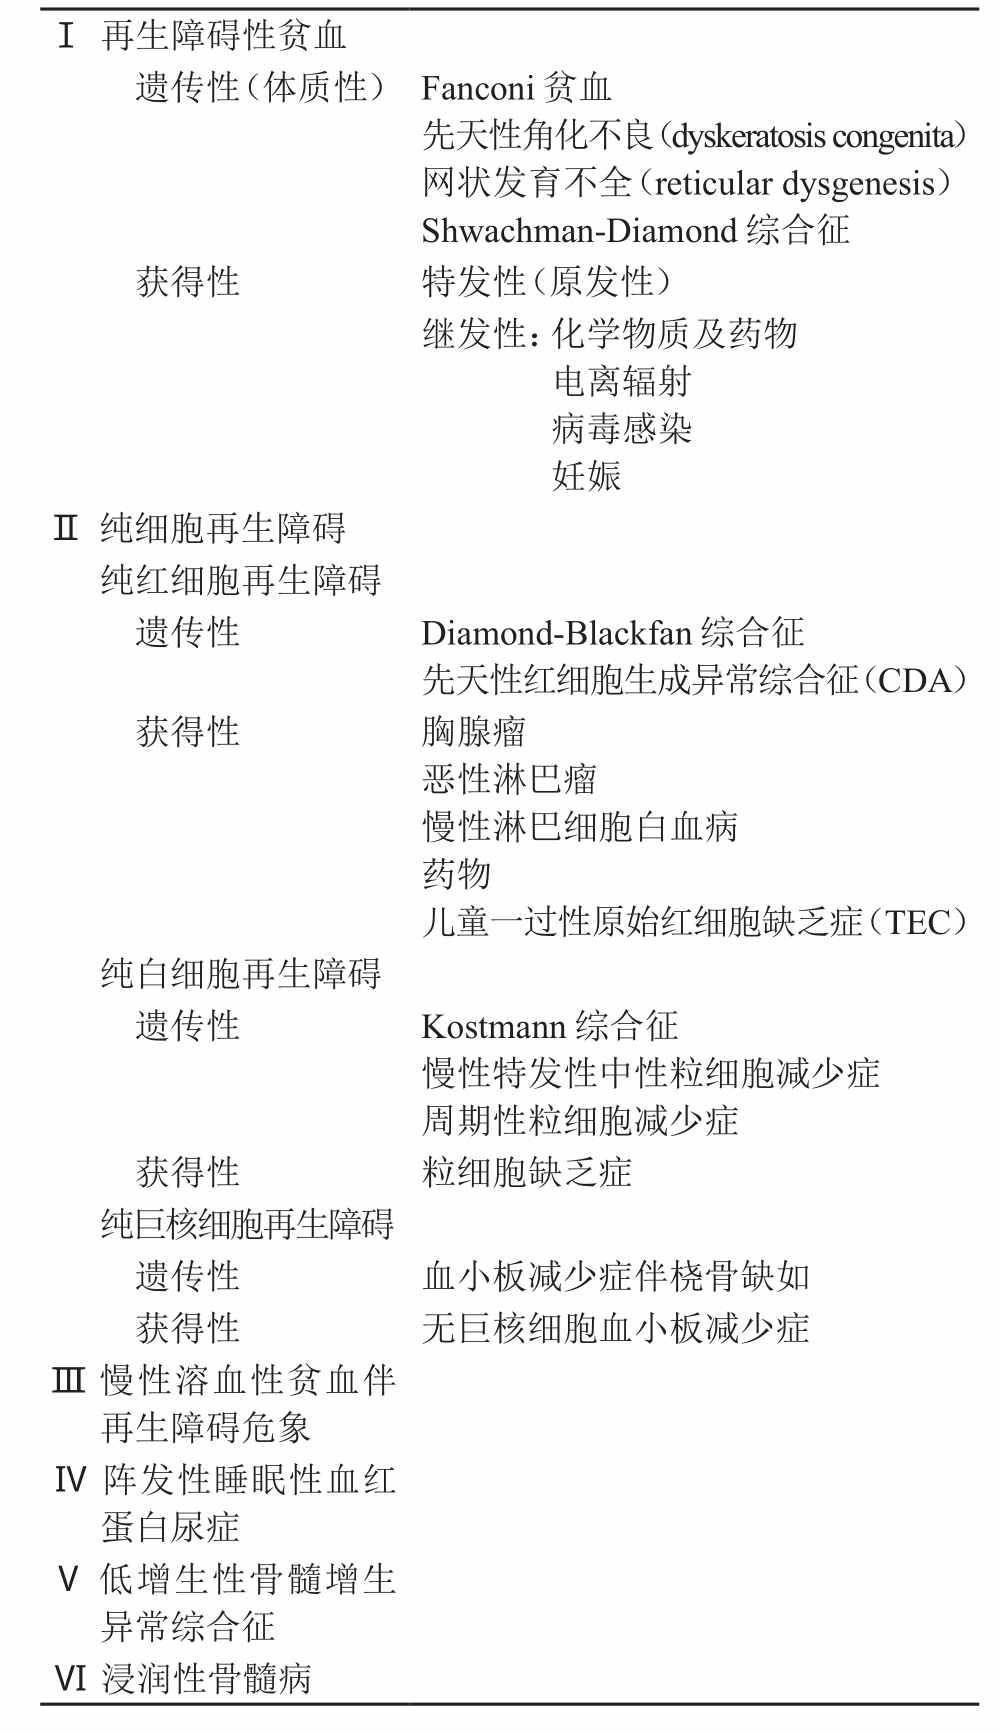
\includegraphics[width=3.33333in,height=5.77083in]{./images/Image00123.jpg}
\end{table}

本章将从临床急诊内科角度,重点阐述各种原因所致的严重型再生障碍性贫血及再生障碍危象。

\section{严重型再生障碍性贫血}

再生障碍性贫血(aplastic
anemia,AA)是指骨髓造血组织显著减少(非骨髓异常浸润和网硬蛋白增加导致)而引起造血功能衰竭的一类贫血,其临床上的严重类型即为严重型再生障碍性贫血(SAA),本病以显著全血细胞减少伴骨髓增生低下为特征。

\subsection{病因与发病机制}

临床上约50\%~75\%的AA病例原因不明为特发性,而继发性病例主要与药物及化学物质、电离辐射、病毒感染及其他因素(如妊娠等)相关。现在已知许多药物可引起AA,氯(合)霉素为药物诱发AA最常见病因,氯(合)霉素骨髓毒性作用与其亚硝基衍生物------亚硝基-氯霉素有关。多种化学物质(如苯、甲苯、杀虫剂及重金属类等)具有骨髓毒性作用。苯的骨髓毒性作用为其代谢产物环氧化苯所致。各种形式的电离辐射均可引发造血干细胞DNA双链断裂而致AA,其效应具有剂量及时间的双重依赖性,大剂量电离辐射还可损害造血微环境中的血管及支持细胞。此外,多种病毒(如肝炎病毒、EB病毒、B\textsubscript{19}
微小病毒、巨细胞病毒及登革热病毒等)感染与AA发生有关,其中病毒性肝炎相关性再障(HAAA)最为多见。AA为病毒性肝炎罕见且严重的并发症之一,常发生于肝炎恢复期或治愈后。肝炎病毒遗传物质可整合到宿主(人类)DNA中,对宿主细胞增殖及分化产生负调控效应,全部或大部分造血干细胞可被破坏,从而导致骨髓造血功能衰竭。AA偶可发生于妊娠时期,称为“妊娠并发的再障”。

目前多数学者认为AA为一组异质性疾病,可能发病机制包括:①原发性或继发性造血干细胞量和(或)质的缺陷;②异常免疫反应损伤造血干细胞;③造血微环境支持功能缺陷;④遗传倾向。目前研究证实所有AA患者存在不同程度造血干细胞量的减少和(或)质的缺陷,如AA患者外周血及骨髓中集落形成细胞显著减少,其造血干细胞在长期骨髓培养体系的正常基质上不能增殖或增殖能力显著降低,且体外对多种造血细胞生长因子刺激的反应性降低等。AA与T淋巴细胞及其分泌的某些造血负调控因子所致的造血干细胞增殖及分化损伤有密切关系,上述损害效应由其骨髓中活化的T淋巴细胞(包括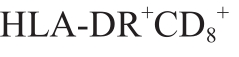
\includegraphics[width=0.78125in,height=0.17708in]{./images/Image00124.jpg}
细胞,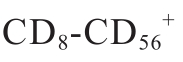
\includegraphics[width=0.59375in,height=0.19792in]{./images/Image00125.jpg}
细胞及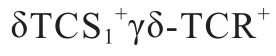
\includegraphics[width=0.90625in,height=0.17708in]{./images/Image00126.jpg}
细胞等)分泌的多种造血负调控因子,如干扰素(IFN)-γ,肿瘤坏死因子(TNF)-α,-β及巨噬细胞炎症蛋白(MIP)-α等介导。某些AA致病因素(如氯霉素)在损害造血干细胞或诱发异常免疫反应同时累及了造血微环境中基质细胞,但大多数AA患者基质层形成完整且迅速,其基质细胞功能缺陷并不多见。值得指出的是,AA虽非典型遗传性疾病,但本病常有HLA-DR\textsubscript{2}
型抗原连锁倾向,儿童病例HLA-DPW\textsubscript{3}
型抗原显著增高,并可见家族性AA,提示AA患者(至少部分AA患者)存在“脆弱”骨髓造血功能遗传倾向。

近两年,端粒及端粒酶在骨髓衰竭发病机制中的作用显得日益重要。研究发现,部分先天性骨髓衰竭疾病造血细胞端粒缩短,端粒酶复合物基因(TERT,TERC,DKC1,NOP10,NHP2,TINF2)突变;约10\%的特发性获得性SAA患者亦有TERT或TERC基因突变及端粒缩短,且与免疫抑制疗效及克隆性演化相关,SAA初次诊断时端粒长度及网织红细胞绝对值是判断患者免疫抑制疗效反应的重要预测指标。

\subsection{诊断}

\subsubsection{临床表现特点}

AA主要临床症状为乏力、出血和感染,为相应血细胞减少所致。SAA起病急骤或在慢性病程基础上病情进一步加重恶化。贫血在病之早期较轻,但呈进行性加剧,并有严重的难以控制的感染,以口腔、咽喉及肛周多见,肺部炎症亦不少见,重者可因脓毒症而死亡。出血症状多见且严重,且常为本病的首发症状,各部位均可出血,以皮肤瘀点、瘀斑、鼻出血及牙龈出血最为多见,其次为消化道、泌尿道及眼底出血,颅内出血亦不少见,可致死亡。体格检查主要表现为皮肤苍白,可见出血点及瘀斑,肝脾及淋巴结一般无肿大。

\subsubsection{实验室检查}

\subparagraph{血象}

表现为严重的全血细胞减少,血红蛋白水平进行性下降,网织红细胞比例<
0.01,其绝对值< 15 × 10\textsuperscript{9}
/L,白细胞总数明显减少,中性粒细胞绝对值< 0.5 × 10\textsuperscript{9}
/L,血小板计数< 20 × 10\textsuperscript{9} /L。

\subparagraph{骨髓象}

多部位骨髓增生减低或重度减低,三系造血细胞明显减少,淋巴细胞比例相对增高,非造血细胞(浆细胞、网状细胞、血窦内皮细胞及组织嗜碱细胞等)增多,巨核细胞明显减少或缺如,骨髓小粒细胞面积<
50\%,以非造血细胞为主,脂肪细胞增多。

\subsubsection{诊断注意事项}

凡有严重贫血,特别是伴有出血及感染症状的患者,血液表现为全血细胞减少,而脾脏无肿大,均应考虑为本病的可能。骨髓检查是诊断本病的主要依据,最好做骨髓活检。遇临床上可疑为本病患者应行多部位骨髓穿刺及活检。有条件单位可做核素\textsuperscript{99m}
Tc、\textsuperscript{113}
In全身骨髓扫描与γ闪烁照相,以了解全身骨髓造血分布情况。临床上本病应与有全血细胞减少的其他疾病,尤其是阵发性睡眠性血红蛋白尿症及骨髓增生异常综合征相鉴别。

\subparagraph{阵发性睡眠性血红蛋白尿症(PNH)}


PNH为一种伴有全血细胞减少的溶血性贫血,临床上易与SAA混淆。但PNH患者可有轻度溶血性黄疸,网织红细胞计数常轻度增高,骨髓中红系细胞增生多活跃,酸化血清溶血试验(Ham试验)常阳性,尿含铁血黄素常持续阳性,如有发作性血红蛋白尿则不难鉴别。但对于受累红细胞<
10\%的PNH,溶血检查常为阴性,不能检测出PNH克隆的存在。补体敏感试验(mCLST)的出现提高了检测PNH的灵敏度。但mCLST只局限于检测受累红细胞,对早期或红细胞未受累的PNH仍无法凭其确定诊断,故流式细胞术分析不同系列造血细胞膜表面GPI蛋白(CD\textsubscript{55}
、CD\textsubscript{59}
)表达已成为PNH诊断及鉴别诊断的金标准。通过GPI锚蛋白及其相应的基因PIG-A的检测,对PNH克隆形成有了较明确的认识。目前认为:PNH克隆是从粒细胞逐渐发展到红细胞,首先受累的是祖细胞;当外周血细胞尚无GPI锚蛋白分子缺陷时,骨髓细胞已可能有GPI锚蛋白分子缺陷,因此检测骨髓细胞比外周血细胞更有意义。同时也使某些临床表现类似再生障碍性贫血、对免疫抑制剂治疗疗效差、实为PNH的患者得到了明确的诊断。

\subparagraph{骨髓增生异常综合征(MDS)}

MDS周围血单核细胞往往增多,并可见幼稚细胞,骨髓增生多活跃,两系或三系细胞呈病态造血,骨髓小粒饱满,以造血细胞为主,通过有核红细胞糖原染色、小巨核酶标、CFU-L及染色体核型等实验室检查有助于与SAA的鉴别。

此外,亦应注意与急性造血功能停滞、骨髓纤维化、急性白血病及恶性组织细胞病等相鉴别。

\subsubsection{诊断标准}

\hypertarget{text00089.htmlux5cux23CHP3-10-1-2-4-1}{}
(一) AA诊断

目前仍沿用1987年第四届全国再生障碍性贫血学术会议修定的诊断标准,具体如下:①全血细胞减少,网织红细胞绝对值减少,淋巴细胞相对增多;②一般无脾肿大;③骨髓至少1个部位增生减低或重度减低(如增生活跃,须有巨核细胞明显减少及淋巴细胞相对增多),骨髓小粒非造血细胞增多(有条件者作骨髓活检等检查,显示造血组织减少,脂肪组织增加);④能除外引起全血细胞减少的其他疾病;⑤一般抗贫血药物治疗无效。

\hypertarget{text00089.htmlux5cux23CHP3-10-1-2-4-2}{}
(二) AA分型诊断

根据上述标准诊断为AA后,再进一步分析是急性AA还是慢性AA。

\subparagraph{急性 AA(亦称SAA-Ⅰ型)的诊断标准}

\hypertarget{text00089.htmlux5cux23CHP3-10-1-2-4-2-1-1}{}
(1) 临床表现:

发病急,贫血呈进行性加剧,常伴有严重感染,内脏出血。

\hypertarget{text00089.htmlux5cux23CHP3-10-1-2-4-2-1-2}{}
(2) 血象:

除血红蛋白下降较快外,须具备以下3项中之2项:①网织红细胞< 1\%,绝对值<
15 × 10\textsuperscript{9} /L;②中性粒细胞绝对值< 0.5 ×
10\textsuperscript{9} /L;③血小板< 20 × 10\textsuperscript{9} /L。

\hypertarget{text00089.htmlux5cux23CHP3-10-1-2-4-2-1-3}{}
(3) 骨髓象:

①多部位增生减低,三系造血细胞明显减少,非造血细胞增多;如增生活跃须有淋巴细胞增多;②骨髓小粒中非造血细胞及脂肪细胞增多。

\subparagraph{慢性 AA的诊断标准}

(1) 临床表现:发病较急性再障缓慢,贫血、感染、出血相对较轻。

(2)
血象:血红蛋白下降速度较慢,网织红细胞、中性粒细胞及血小板减低,但达不到急性再障的程度。

(3)
骨髓象:①三系或两系减少,至少一个部位增生不良,如增生活跃,则淋巴细胞相对增多,巨核细胞明显减少;②骨髓小粒中非造血细胞(如脂肪细胞等)增加。

(4) 病程中如病情恶化,临床、血象及骨髓象与急性AA相同,称SAA-Ⅱ型。

\subsection{治疗}

SAA属于难治性血液病,本病进展迅速,预后凶险,自然病程6个月左右,20世纪70年代以前由于无有效治疗方法,依靠常规药物治疗如雄性激素、莨菪类药物、马钱子碱及一叶萩碱等,3个月病死率高达90\%,死亡原因多为脑出血及严重感染,少数患者死于急性左心衰竭。近年来由于新的治疗方法不断涌现,如异基因骨髓移植、抗淋巴细胞球蛋白/抗胸腺细胞球蛋白、环孢素A、环磷酰胺、丙种免疫球蛋白、重组人造血细胞生长因子以及支持疗法的进一步加强,已使SAA的治疗效果及预后大为改观。

\subsubsection{支持治疗}

良好的支持治疗是保证患者可获得进一步治疗的基础。

\hypertarget{text00089.htmlux5cux23CHP3-10-1-3-1-1}{}
(一) 感染及出血的防治

良好的护理及积极对症处理对于预防和控制感染及出血极为重要
。不应忽视常规预防性措施,如口腔清洁护理、便后坐浴及空气消毒等,有条件可设置无菌隔离室或层流病房。早期发现局部及隐匿性感染灶,并积极处理。目前不主张采用预防性全身抗生素治疗,应尽量减少肌肉注射,如需要,也应谨慎给药。感染确定后应用特异性抗生素进行治疗,不明原因的发热,经适当的检查后可用广谱抗生素直至诊断明确为止。对于严重不易控制的感染,可加以输注入丙种球蛋白,粒细胞集落刺激因子(G-CSF)对控制感染亦有所帮助。出血倾向明显者应针对性给予止血剂及输注血小板。

\hypertarget{text00089.htmlux5cux23CHP3-10-1-3-1-2}{}
(二) 输血

由于输血可影响到将来的治疗和最终的生存,故输血应谨慎并恰当应用成分血液治疗。输注浓缩红细胞的主要目的是维持患者良好自觉状态,而不一定维持一定的血红蛋白水平。输血的危险性值得注意,如输血相关性肝炎及含铁血黄素沉着症,此外还可造成红细胞抗原和移植抗原的致敏。有严重出血时应给予浓缩血小板输注,感染的存在可降低血小板输注的疗效。如果患者发生血小板无效输注,则应输注HLA相合的血小板。如考虑骨髓移植,家族成员也应避免作为供血者,因为患者可能因此而对次要的移植抗原致敏。不应预防性给予白细胞输注,然而对于伴严重革兰阴性杆菌感染的粒细胞缺乏患者,白细胞输注可能有辅助治疗价值。

\subsubsection{骨髓移植(BMT)}

BMT是SAA的一种有效治疗方法,至今已有数千例SAA患者接受了此种治疗,其中60\%~80\%患者恢复正常造血并长期生存。

\hypertarget{text00089.htmlux5cux23CHP3-10-1-3-2-1}{}
(一) 目的

BMT的目的是使功能正常的造血干细胞植入患者体内,以取代原有缺陷的造血干细胞,重建患者的骨髓造血功能及免疫功能。

\hypertarget{text00089.htmlux5cux23CHP3-10-1-3-2-2}{}
(二) 患者及供体选择

\subparagraph{患者选择}

因为目前BMT失败可能性不小,且费用昂贵,因此必须严格掌握如下适应证:①SAA-Ⅰ型/Ⅱ型;②患者年龄小于35~40岁,最大年龄不应超过45岁;③有HLA相合的同胞兄弟姐妹做供体,无HLA相合的同胞供者严格掌握适应证后可选择无关供者骨髓移植做为二线解救治疗;④既往无或少许输注血液制品史的早期患者;⑤无明显感染迹象。

\subparagraph{供体选择}

①同卵孪生子(称为同基因骨髓移植,Syn-BMT);②HLA相合的同胞兄弟姐妹(即异基因骨髓移植,Allo-BMT);③替代供体:近年来由于家庭人口数的减少,大多数SAA患者找不到HLA匹配的同胞,这促使替代供体(HLA匹配的无关供体及HLA不匹配的亲属供体)BMT研究工作的进展,但目前用此类供体进行BMT的成功率较低,尚无理想的预处理方案及移植物抗宿主病(GVHD)预防方案。

作为供体应无输血史及妊娠史,无传染病,且经解释后对供髓有充分理解后同意自愿献髓。

\hypertarget{text00089.htmlux5cux23CHP3-10-1-3-2-3}{}
(三) 适应证

\subparagraph{HLA相合的同胞供者骨髓移植}

新诊断的SAA患者如符合下列条件应首选同种异基因骨髓移植:①SAA或极严重型AA(即VSAA,指中性粒细胞<
0.2 × 10\textsuperscript{9}
/L)患者;②年龄小于40岁;③有HLA相合的同胞供者;④儿童非重型再障但有明确治疗指征应首选HLA相合同胞供者骨髓移植。

\subparagraph{HLA相合的无关供者骨髓移植}

①在DNA水平达到HLAⅠ类和Ⅱ类抗原完全相合;②年龄小于50岁,50~60岁患者如果身体状态良好亦可考虑;③符合SAA
或VSAA标准;④至少一疗程ATG联合CsA治疗失败后的儿童或成人患者,成人一疗程ATG联合CsA失败后根据个体情况亦可考虑二次ATG治疗;⑤骨髓移植时无活动性感染或急性出血表现;⑥无HLA相合同胞供者的先天性再障患者。

\hypertarget{text00089.htmlux5cux23CHP3-10-1-3-2-4}{}
(四) BMT的时机

一旦确诊为SAA,或VSAA的年轻患者有HLA相合供体,首选Allo-BMT,且应尽早进行,以避免因输血使患者对献血员次要组织相容性抗原致敏,导致移植排斥发生率升高,降低移植成功率及长期存活率。患者在等待供者选择过程中可先用环孢素A加GM-CSF或G-CSF,一旦有合适供者,立即移植。

儿童或成人SAA经一疗程ATG联合CsA治疗后4~6个月评估失败患者,可以考虑全相合无关供者骨髓移植,成人患者根据个体情况亦可行二次ATG治疗。

\hypertarget{text00089.htmlux5cux23CHP3-10-1-3-2-5}{}
(五) 骨髓的采集及输注

骨髓的采集宜在输注当天进行,采髓总量以骨髓有核细胞计,一般不应少于3 ×
10\textsuperscript{8}
/kg患者体重。为使供者避免感染肝炎、艾滋病等病毒的危险,在采髓过程中不应输库存血,可在采髓前2周之内分次采供者自身血600~800ml保存,供采髓术中用。采集的骨髓经80~100目不锈钢网大容量骨髓过滤器过滤后就可直接从静脉输入受者体内,需注意勿将浮在骨髓液面上的脂肪一并输入。骨髓输注时间一般在预处理结束24~48小时开始,输注速度与输血相同,输注前给予适量皮质激素。

\hypertarget{text00089.htmlux5cux23CHP3-10-1-3-2-6}{}
(六) 预处理

CTX与抗胸腺细胞球蛋白(ATG)联合预处理方案目前已被公认为SAA
Allo-BMT的最佳预处理方案。具体方法如下:CTX
50mg/(kg•d),共4天,在第1,2,3剂CTX 后12小时给予ATG
30mg/kg,静脉输注10~12小时,在最后1剂CTX后36小时输髓。为减少ATG副作用,于ATG输注前应用甲泼尼龙2mg/kg。西雅图骨髓移植中心应用CTX/ATG方案对39例SAA患者进行了HLA匹配同胞供体Allo-BMT,结果仅2例(5\%)发生移植排斥(GR),且2例患者二次Allo-BMT均获成功,3年实际存活率高达92\%,显著高于前期年龄及GR危险因素相似的39例对照患者(72.0\%)(P
= 0.043)。

\hypertarget{text00089.htmlux5cux23CHP3-10-1-3-2-7}{}
(七) 移植后并发症处理及其预防

\subparagraph{移植排斥}

SAA患者Allo-BMT后移植排斥仍是移植失败的主要原因。移植排斥有两种形式,第一种形式为早期移植排斥,即BMT后始终未见有受者造血功能重建的证据,这种情况多发生在移植后头3~4周;第二种形式称晚期移植排斥,这类患者移植后造血功能曾有不同程度恢复,且出现了供受者混合型嵌合体,但随着移植后时间的推延,植入供者的造血干细胞又逐渐被排斥,或者在停用免疫抑制剂如环孢素A(cyclosporin
A,CsA)后发生,这种情况多发生在移植后几周至几月。移植排斥多见于单用CTX预处理方案的BMT,可能由先前输血使受体细胞对供体细胞上表达的次要组织相容性抗原致敏引起,因此,对BMT前有多次输血史的患者应当加强预处理。此类患者如果单用CTX预处理,排斥率高达30\%~45\%。目前大多数中心采用以下几种方案以降低有多次输血史的SAA患者排斥率:①CTX
+照射,如CTX +全身照射(TBI,300CGy)或CTX
+全淋巴系照射(TLI,750CGy)或CTX
+屏蔽双肺的胸腹联合照射(TAI,600CGy),排斥率可降低至3\%左右,采用照射虽然可以减少排斥反应,但GVHD及间质性肺炎发病率增加,故未能改善患者的生存率;②CTX
+供体白膜输注,此方案只能促进植入,但增加了严重急性尤其是慢性GVHD的发生率,从而降低了生存率,近年来大多数中心已不再采用此方案;③CTX
+ ATG,为一种很有前途的预处理方案,可将排斥率降低至3\%左右;④CTX +
CsA,以CsA代替MTX预防GVHD的同时,亦使排斥率降低至10\%左右,但在CsA停用时有些患者会发生晚期排斥,因此,CsA的合理应用是从移植的前一天开始2~5mg/(kg•d)静脉输注,连用10~12个月,必要时可进一步延长,根据CsA肾毒性,排斥反应控制情况及血药浓度调整CsA的用量。CTX
+ ATG及CTX +
CsA为目前较为理想的可明显降低移植排斥的预处理方案。近几年来,由于输注处理过的血液制品(去除白细胞的红细胞及血小板,血液制品输注前给予20~24Gy照射)增加,患者移植较早,BMT前输血减少,输注的骨髓有核细胞数增加以及CsA的广泛应用,移植排斥的危险已明显降低。

由于植入失败病死率极高,一经确诊应考虑进行第二次BMT,目前较理想的第二次BMT预处理方案为CTX
+ ATG。二次移植时间宜>
60天。若第二次移植时改用另一位HLA匹配同胞兄弟姐妹做供者,则移植成功率可进一步提高。

\subparagraph{移植物抗宿主病(GVHD)}


GVHD分为急性与慢性,是SAA患者BMT后一种常见并发症,也是移植相关性死亡中最常见的原因。

\hypertarget{text00089.htmlux5cux23CHP3-10-1-3-2-7-2-1}{}
(1) 急性GVHD:

急性GVHD一般发生在移植后14~45天,发生≥Ⅱ度急性GVHD患者只有40\%~45\%获长生存,而无或仅Ⅰ度急性GVHD患者长生存达85\%。与急性GVHD发生有关的危险因素主要有:①单用MTX比CsA
+
MTX预防发生率高;②GVHD随受者年龄增大而增高;③供髓者有妊娠史;④移植后加用供者白细胞层细胞(buffy
coat);⑤HLA不相符程度。基于目前对GVHD无特别有效的治疗方法,因此对SAA患者应加强GVHD的预防。以前最基础的GVHD预防方案为MTX,自20世纪70年代末期CsA应用以来,其对GVHD预防作用引起了人们重视,临床随机研究比较了MTX及CsA
+
MTX两方案预防GVHD,结果表明Ⅱ~Ⅳ度GVHD发病率前者(53\%)明显高于后者(18\%),而且后者中无Ⅳ度GVHD,2年实际生存率分别为60\%及82\%,此说明CsA与短期MTX联合应用能降低急性GVHD的发病率及严重性。迄今为止,CsA(用法同前)+短期MTX(MTX
+ 1天10mg/m\textsuperscript{2} ,静脉输注,+ 3天,+ 6天及+
12天为6mg/m\textsuperscript{2}
)为预防GVHD最佳方案。目前预防GVHD其他措施还有:①所有血液制品用20~24Gy放射线照射,以灭活具有免疫活性的T淋巴细胞;②将患者置于空气层流洁净室;③无菌饮食及口服肠道非吸收抗生素,因为细菌和人的上皮细胞具有某些相同表面抗原,在皮肤和肠道繁殖的细菌有刺激引起急性GVHD的作用;④用抗T淋巴细胞单克隆抗体去除供髓中的T淋巴细胞等(但会增加移植排斥)。一旦发生GVHD,适当增加CsA剂量,使CsA血药浓度维持在300~450ng/ml,并加用糖皮质激素。

\hypertarget{text00089.htmlux5cux23CHP3-10-1-3-2-7-2-2}{}
(2) 慢性GVHD:

慢性GVHD一般发生在移植后100天,是一明显影响生存率的并发症。鉴于慢性GVHD多发生于CsA减量时,对于年龄>
32岁,BMT中输注过供体白细胞,发生过急性GVHD,BMT前有感染,预处理方案中包含照射等有发生慢性GVHD高危因素的患者或许会受益于以后较长时间应用治疗水平的CsA,并辅以糖皮质激素,可使慢性GVHD延迟发生或完全避免。

\subparagraph{间质性肺炎(IPn)}

IPn是SAA患者BMT后常见并发症之一,其发病率及死亡率分别为17\%及11\%。BMT后用MTX而不用CsA预防GVHD,中、重度急性GVHD,预处理方案中包含TBI,受体年龄>
20岁等患者易发生IPn。近年来由于MTX及TBI的应用减少,IPn的发病率也相应明显下降。

其他并发症如出血性膀胱炎少见。BMT后长期生存者有发生继发性实体瘤的危险,尤其是预处理方案中用TBI者。

\hypertarget{text00089.htmlux5cux23CHP3-10-1-3-2-8}{}
(八) 疗效

自 1969年在西雅图成功地进行了首例
Allo-BMT治疗SAA患者以来,Allo-BMT治疗SAA的疗效不断提高并已获重大进展。来自西雅图骨髓移植中心资料显示,Allo-BMT后SAA患者生存率由1970~1976年间45\%增至1977~1988年间的60\%,并于1988~1993年间升达90\%以上。Allo-BMT治疗SAA疗效逐年提高得益于以下因素:不断改良的预处理方案明显降低了GR发生率;将长期单用甲氨蝶呤(MTX)改为短疗程MTX加长疗程环孢素A(CsA)不仅有效预防和减少了急、慢性GVHD发生率,亦能促进植活;输注处理过的血液制品(如少白细胞的红细胞及血小板)可避免或减少同种致敏;多种新型高效抗生素及抗病毒药物问世使得支持治疗进一步加强。大量结果显示Allo-BMT疗效与患者年龄有关,来自欧洲BMT协作组(EBMT)1990~1998年间资料表明,接受Allo-BMT
的16岁以下,17~40岁和大于40岁3个年龄组患者5年存活率分别为77\%、68\%和54\%,EBMT建议将SAA接受Allo-BMT的上限年龄定为45岁。其他影响疗效的不良因素包括:移植前输血多、诊断至移植时间长、供受者性别不合(尤指有妊娠史或输血史的女性供者给男性患者)、移植后输注供者的白细胞,GVHD预防方案不含CsA等。此外,不采用含照射预处理方案及避免应用硫唑嘌呤治疗慢性GVHD可减少或避免Allo-BMT相关的继发性恶性肿瘤发生的危险性。

\subsubsection{免疫抑制治疗}

大量临床研究相继报道抗淋巴细胞球蛋白(ALG)/抗胸腺细胞球蛋白(ATG)、环孢素A(CsA)等单用或与其他免疫抑制剂(如甲泼尼龙、皮质类固醇等)联合应用治疗SAA疗效确切,与雄性激素及重组人造血细胞生长因子联合应用有助于进一步提高疗效。

\hypertarget{text00089.htmlux5cux23CHP3-10-1-3-3-1}{}
(一) ALG/ATG

ALG/ATG是用人胸导管淋巴细胞或胸腺淋巴细胞免疫兔、马、猪等异种动物,再经人血小板和红细胞吸附去除杂抗体,然后层析提纯制取的一种抗血清,主要为IgG,它是一种对免疫活性细胞和造血细胞具有多种作用的多克隆生物活性免疫调节剂。

\subparagraph{适应证}

①年龄≤40岁的SAA或VSAA,但无合适的HLA相合同胞供者行异基因骨髓移植;②年龄>
40岁的SAA或VSAA患者;③非重型再障患者但严重依赖红细胞和(或)血小板输注;④非重型再障患者虽没有血制品输注依赖,但有严重中性粒细胞缺乏伴有潜在严重感染风险。

\subparagraph{治疗方法}

ALG或ATG主要用于治疗SAA。用法是静脉试验阴性后,按兔ALG(或ATG)3~5mg/(kg•d),猪ALG(或ATG)20~30mg/(kg•d),马ALG(或ATG)12~15mg/(kg•d),掺入1000ml生理盐水或5\%葡萄糖液中缓慢静脉滴注(维持12~16小时)。疗程一般为4~5天,亦有连用7天、10天或更久者。对于一个疗程后观察3个月或以上没有明显疗效;或曾经有效后复发的患者,可以考虑应用第二疗程ALG(或ATG),此时应更换ALG(或ATG)制剂的动物来源,以免发生严重过敏反应。此外,ALG/ATG治疗期间患者应住隔离病室,并口服肠道不吸收抗生素,以减少外源性和肠道感染的机会。出现感染指征时应及时给予抗生素治疗。为补偿ALG(或ATG)所引起的血小板消耗,防治危及生命的严重出血,可据病情(或每天)输注血小板。为预防过敏反应和血清病,还需常规给予肾上腺皮质激素{[}相当于泼尼松1mg/(kg•d){]}及抗组织胺类药物等。目前国内外常用的治疗方案有:①ALG/ATG单用;②ALG/ATG加雄性激素;③联合免疫抑制剂的治疗,即ALG/ATG联合CsA/(大剂量)6-甲泼尼龙(6-Mpred);④免疫抑制剂与重组人造血细胞生长因子(rhHGFs)联合应用。

\subparagraph{疗效}

早期多组前瞻性随机临床研究比较了ALG/
ATG与传统治疗(支持治疗及雄性激素)治疗SAA的疗效。ALG/ATG单用治疗SAA的有效率为28\%~67\%,2年生存率为62\%~76\%,与传统支持治疗及雄性激素相比,ALG/ATG可显著提高有效率,延长生存期。

雄性激素和ALG/ATG已被证实是治疗SAA的有效药物,两者合用可获得更好疗效。虽然有的学者认为雄性激素与ALG/ATG联合应用不会提高SAA患者对ALG/ATG的反应,但多数学者认为ALG/ATG与雄性激素联合应用能明显提高疗效。SAA患者ATG治疗后,其疗效有赖于雄性激素的维持治疗,多组学者用此法治疗SAA的疗效见表\ref{tab34-2}。

\subparagraph{ALG/ATG治疗反应的预测因素}

\begin{table}[htbp]
\centering
\caption{ALG/ATG加雄性激素前瞻性治疗SAA的疗效}
\label{tab34-2}
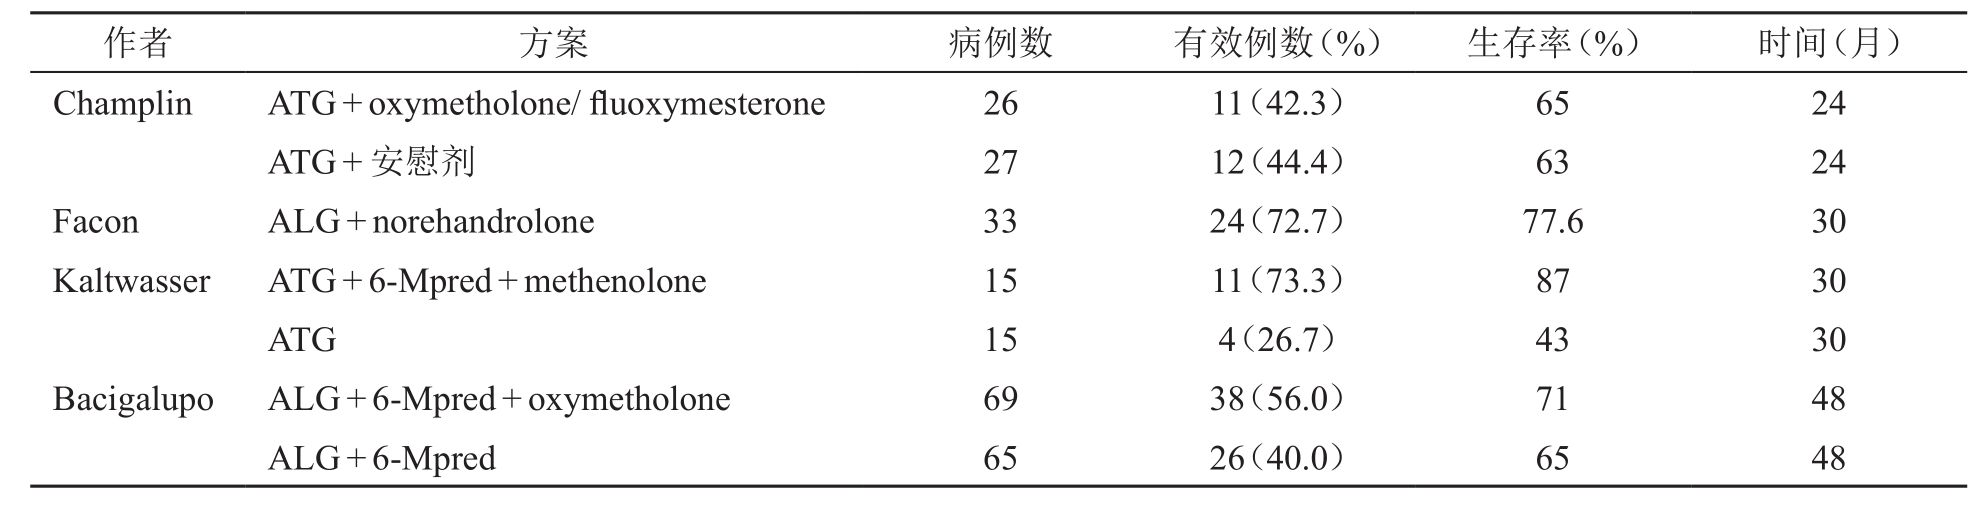
\includegraphics[width=6.60417in,height=1.67708in]{./images/Image00127.jpg}
\end{table}

众多回顾性分析结果表明,患者年龄、性别、病因及既往治疗与生存率无相关性。Marsh等研究表明:患者种族、输血史、骨髓细胞增生度、骨髓中淋巴细胞比例以及外周血淋巴细胞水平与生存率亦无相关性。但有研究显示,治疗前外周血细胞水平,红细胞平均体积(MCV)及病程与ALG/ATG疗效相关。网织红细胞(RC)绝对值>
10 × 10\textsuperscript{9} /L及中性粒细胞绝对值(ANC)> 0.2 ×
10\textsuperscript{9} /L者,生存率较高;血小板水平(BPC)< 10 ×
10\textsuperscript{9} /L者,生存率低;病程<
2个月者有效率及生存率均增高。相反来自美国多中心的研究发现,年轻患者、ANC
< 0.2 × 10\textsuperscript{9}
/L、女性及病因不明确者预后更好,生存率提高;而未发现RC、BPC、MCV及病程与疗效存在相关性。Nissen等发现,10岁以下女孩患者治疗后血液学恢复明显延迟。Halperin报道,儿童SAA患者ALG/ATG有效率仅为25\%。Bacigalupo等认为,就诊时ANC与生存率显著相关(P
< 0.000 01)。总之,目前尚未能找到预测ALG/
ATG疗效的理想临床参数及体外实验指标,但多数学者认为,年轻(<
20岁)的超重型AA(ANC < 0.2 × 10\textsuperscript{9}
/L)患者疗效极差;治疗前外周血细胞水平高者,ALG/ATG治疗后骨髓造血功能恢复的可能性更大。

\subparagraph{ALG/ATG近期副作用}

ALG/ATG治疗最初几天,大多数患者可出现发热、寒战、多形性皮疹、低血压/高血压;治疗过程中可引起血小板及中性粒细胞减少、出血加重、血小板输注需求量明显增加;较少见的副作用包括:毛细血管渗漏综合征、溶血、心律失常及癫痫发作;如果ALG/ATG经周围静脉输注,可发生静脉炎;治疗后7~10天约60\%患者可发生血清病,其常见症状有:反复发热、皮疹、胃肠道症状、肌痛、关节痛及蛋白尿等,严重时可危及生命,血清病发病率取决于ALG/ATG类型、剂量及疗程;肝肾毒性极少见。ALG/ATG治疗期间需严密监护,应用小剂量皮质类固醇可减轻或预防绝大多数急性副作用。

\subparagraph{ALG/ATG治疗患者晚期并发症}

通过对ALG/
ATG治疗的SAA患者长期随访,发现相当一部分可发生晚期并发症:晚期复发,演变为克隆性疾病如阵发性睡眠性血红蛋白尿症(PNH)、骨髓增生异常综合征(MDS)及急性髓细胞白血病(AML)。中国医学科学院血液病医院总结了16年间802例AA经免疫抑制治疗后克隆演变的情况,免疫抑制治疗后5年克隆演变发生率为3.7\%,其中演变为MDS/AML或PNH的发生率分别为1.7\%和2.1\%,VSAA患者发生克隆演变的相对危险度7倍于SAA和非重型再障患者,而后两者间无显著差异。EBMTSAA工作组对719例接受免疫抑制剂治疗SAA患者进行了回顾性分析,其中358例(49.8\%)有效,74例(10.3\%)复发,复发平均时间为778天,14年实际复发率高达35.2\%。笔者统计了3篇关于SAA患者ALG/ATG治疗后晚期克隆性疾病发病率的报道,随访病例共计451例,其中70例(15.5\%)发生了克隆性疾病:40例(8.9\%)转变为PNH,22例(4.9\%)演变为MDS,7例(1.6\%)进展为AML,1例(0.2\%)发展为淋巴瘤;De
Planque等随访发现克隆性疾病发生的中位时间为:PNH 3年,MDS
4.6年,AML时间则更长。Tichellli等估计,ALG/ATG治疗后8年晚期克隆性疾病发病率高达57\%,并认为上述并发症很可能是由于体内残留损害的骨髓造血干细胞进一步发展所致。

\subparagraph{ALG/ATG的疗效机制}

ALG/ATG具有T细胞及非T细胞的细胞毒性免疫抑制作用,能去除抑制性T细胞对骨髓造血抑制作用,ATG治疗前收集的外周血CD\textsubscript{8}
\textsuperscript{+} 细胞能够明显抑制SAA患者骨髓CD\textsubscript{34}
\textsuperscript{+}
细胞的BFU-E及CFU-GM生长,而ATG治疗后恢复期患者外周血CD\textsubscript{8}
\textsuperscript{+}
细胞的造血抑制活性消失。ATG治疗有效患者外周血IL-2受体\textsuperscript{+}
(IL-2R\textsuperscript{+}
)细胞数量显著减少,故推测IL-2R\textsuperscript{+}
细胞可能是ATG作用的靶细胞。ALG/ATG亦是一种免疫刺激剂,具有类似植物血凝素但较之更强的致丝裂原作用,能促进淋巴细胞增殖,从而增加HGFs,如IL-3,GM-CSF合成及释放。患者对ALG疗效反应与其刺激的外周血单个核细胞(PBMNC)合成GM-CSF量成正相关。此外,ALG/
ATG还可作用于造血干/祖细胞表面受体,如CD\textsubscript{45}
RO等,直接刺激造血干/祖细胞生长或使它对HGFs敏感性增高。ALG/ATG的疗效可能来源于上述选择性刺激/抑制综合效应,后者能产生其他免疫抑制疗法及rhHGFs所不能达到的治疗作用,此观点与临床上SAA患者经ALG/ATG治疗后获较缓慢而持久的造血功能恢复相吻合。

\subparagraph{ALG/ATG初始治疗无效或复发患者的处理原则}

包括:①二次ALG/ATG(更换制剂动物来源);②改用其他免疫抑制剂如CsA等;③rhHGFs;④Allo-BMT;⑤CsA加大剂量静脉丙种球蛋白;⑥雄性激素及加强支持治疗。既往由于顾虑可能发生严重血清病反应而避免二次应用ALG/ATG;现在广泛应用小剂量皮质激素可显著减少其发生率,并使二次甚或多次ALG/ATG治疗成为可能。初步结果表明:20\%~40\%患者经二次ALG/ATG治疗后可获缓解。来自瑞士单一研究中心对第一疗程ALG无效或复发的患者实施重复疗程ALG治疗的可行性及其疗效进行了评价。1976~1995年间139例初诊SAA患者序贯接受了ALG治疗,89例患者对第一疗程ALG有反应,其余50例未能脱离输血。89例有效患者中66例获持续缓解,另外23例复发。43例患者因第一疗程无效(25例)或复发(18例)而接受第二疗程(35例),第三疗程(6例)甚至第四疗程(2例)ALG治疗,共计53疗程。结果显示,第一疗程与重复疗程ALG治疗期间急性并发症的发生率分别为26\%及30\%(P
> 0.2),其血清病反应发生率亦无差异性,分别为63\%及57\%(P >
0.2),但后者血清病反应出现时间(中位时间6天)明显早于前者(中位时间13天)(P
=
0.008)。接受重复疗程ALG治疗的43例患者中27例(63\%)脱离输血,第一疗程无效及复发患者对重复疗程ALG治疗的反应率分别为64\%及61\%,本组患者10年生存率达52\%
±
8\%。接受单一疗程及重复疗程ALG治疗患者20年晚期克隆性疾病发病率分别为34\%
± 7\%及53\% ± 10\%(P =
0.15)。上述结果显示重复疗程ALG不仅疗效满意,且具良好安全性。

\hypertarget{text00089.htmlux5cux23CHP3-10-1-3-3-2}{}
(二) CsA

CsA是由真菌Tolypocladium
infatum生成的环形内十肽,作为一种特异性强力免疫抑制剂,CsA已广泛用于器官移植及多种自身免疫性疾病。近10年来,国内外学者应用CsA治疗AA亦获得满意疗效。

\subparagraph{治疗方法}

CsA单用时,多采用大剂量口服用药,其推荐剂量成人为12mg/(kg•d),儿童为15mg/(kg•d),用药60天后逐渐减量,小剂量长期服用对维持疗效,减少疾病复发非常有利。

\subparagraph{疗效}

早期文献报道CsA治疗SAA的疗效颇不一致,有效率为15\%~75\%不等。法国多中心治疗研究结果显示,CsA和ATG分别作为SAA的最初治疗,其3个月及12个月时有效率及生存率均无差异性。此外,CsA可使ALG/ATG难治的SAA产生50\%的反应率。需要指出的是,由于过敏、血小板严重减少或白细胞重度低下对ALG/
ATG难以耐受的SAA患者可考虑首先应用CsA治疗。

\subparagraph{CsA毒副作用}

CsA主要毒副作用为肾毒性。其他还有消化道反应、多毛症、手颤、高胆红素血症及末梢感觉异常等。为了尽量减少毒副作用,初始剂量宜小{[}如3~5mg/(kg•d){]}以后逐渐递增剂量,用药期间监测血药浓度及血浆肌酐水平,以血药浓度维持在200~400ng/ml为宜,若血浆肌酐上升超过基础水平的30\%,则应减量。

\subparagraph{CsA的远期并发症}

单用CsA治疗的SAA发生晚期克隆性疾病的危险性并不增加。最近Ohara等对167例儿童SAA进行了回顾性分析,结果显示发生晚期克隆性疾病(MDS/AML)的危险性与同时并用CsA与rhuG-CSF治疗高度相关:11/50例接受CsA并用rhuG-CSF治疗的患者发生MDS/AML,而单用CsA或rhuG-CSF治疗(共41例)及接受Allo-BMT治疗(48例)患者无1例发生MDS/AML。

\subparagraph{CsA疗效反应的预测因素}

CsA疗效反应有利因素包括初诊时骨髓单个核细胞干扰素(lFN)-γ
mRNA(+);HLAⅡ类单体型呈DRB1*1501-DQA1*0102-DQB1*0602;患者初诊时骨髓红∶粒系细胞比值(E/G比值)高者(>
0.6);血清IL-2与可溶性IL-2R水平增高。

\hypertarget{text00089.htmlux5cux23CHP3-10-1-3-3-3}{}
(三) 强化免疫抑制治疗

联合应用不同作用机制的免疫抑制剂可能产生协同效应,从而有助于提高疗效;此外,联合应用可降低各种免疫抑制剂的剂量,从而提高患者的耐受能力。最近临床研究表明,在SAA的治疗中,强化免疫抑制治疗(IIST)明显优于ALG/ATG治疗(表\ref{tab34-3})。

\hypertarget{text00089.htmlux5cux23CHP3-10-1-3-3-4}{}
(四) 免疫抑制剂与rhHGFs联合应用

SAA患者ALG/ATG治疗失败的主要原因为并发严重感染所致的早期死亡,ANC < 0.2
× 10\textsuperscript{9}
/L者尤为危险。合并应用rhHGFs可能促进中性粒细胞水平的迅速恢复,以达到降低感染相关性死亡之目的。

EBMT SAA工作组设计下述方案治疗100例SAA患者:

ALG 15mg/(kg•d),第1~5天;

6-Mpred 2mg/(kg•d),第1~5天;

CsA 5mg/(kg•d),第1~180天;

rhG-CSF 5μg/(kg•d),第1~90天。

治疗前中性粒细胞中位数为0.2 × 10\textsuperscript{9}
/L,应用上述治疗后最高白细胞数< 5 × 10\textsuperscript{9}
/L、(5~14)× 10\textsuperscript{9} /L及> 14 × 10\textsuperscript{9}
/L者的无效率分别为63\%、13\%及4\%,死亡率分别为42\%、8\%及0\%。77例(77\%)骨髓三系细胞恢复良好;中数随访期1424天(81~2889天),5年实际生存率87\%。上述结果表明,免疫抑制剂联合rhHGFs不仅降低了感染死亡率,且有助于造血功能恢复。

来自欧洲的一个前瞻性随机对照研究结果显示,ALG + CsA +
rhG-CSF治疗组中性粒细胞早期升高,其严重感染率相对较低,但较之ALG +
CsA治疗组,两者间2年有效率及存活率均无明显差异。鉴于此,有必要进行更大系列的前瞻性随机对照研究以明确rhHGFs在SAA治疗中的价值。

\subsubsection{其他疗法}

\subparagraph{大剂量环磷酰胺(HD-CTX)}

CTX为一种烷化剂,能降低外周血淋巴细胞数量,抑制机体的免疫反应。1996年Brodsky报告用大剂量CTX{[}45mg/(kg•d),共4
天{]}治疗10例SAA,长期随访的结果,除3例无效外,7例获长期持续性缓解,无复发和发展为克隆性疾病。随后,Tisdale等进行一个抽样试验,比较ATG和CTX初治SAA疗法的疗效。24例患者随机抽样分组,CTX
50mg/kg或ATG
40mg/kg,连用4天,两者均合用6个月的CsA治疗,结果两组有效率无明显差别,但接受CTX治疗的患者需要更强有力的支持治疗。近期应用HD-CTX{[}20mg/(kg•d)共4天{]}治疗5例SAA,3例于短期(3个月内)即获缓解,初步疗效令人满意。上述结果表明CTX是一个有治疗前景的药物,但运用这种毒性大的药物是否合理,尚需进行更大的抽样试验和长期随访来决定。HD-CTX治疗期间,应分别在应用CTX的0小时、3小时、6小时、9小时输注美司那进行解救,同时加强碱化利尿,液体输注量以3000ml/m\textsuperscript{2}
为宜,维持尿pH于7.0左右。

\subparagraph{大剂量甲泼尼龙(HDMP)}

Bacigalupo等(1980)首先报道HDMP治疗SAA,一般剂量为20mg/(kg•d),静脉输注,每隔3~4天半量递减,疗程为30~45天。其疗效不及ALG/ATG或CsA,不良反应较明显,可引起高血压、低血钾、激素性尿糖、库欣综合征、精神症状等,且易并发肺炎、败血症等严重感染。目前多与其他药物组成联合方案使用。

\subparagraph{大剂量免疫球蛋白(HDIg)}

1985年Atrah等用于SAA,剂量为0.4~1g/(kg•d),静脉输注,疗程为3~5天。较适用于合并感染、出血严重患者,副作用少见。

\subsubsection{SAA的治疗选择策略}

\begin{table}[htbp]
\centering
\caption{SAA的强化免疫抑制治疗}
\label{tab34-3}
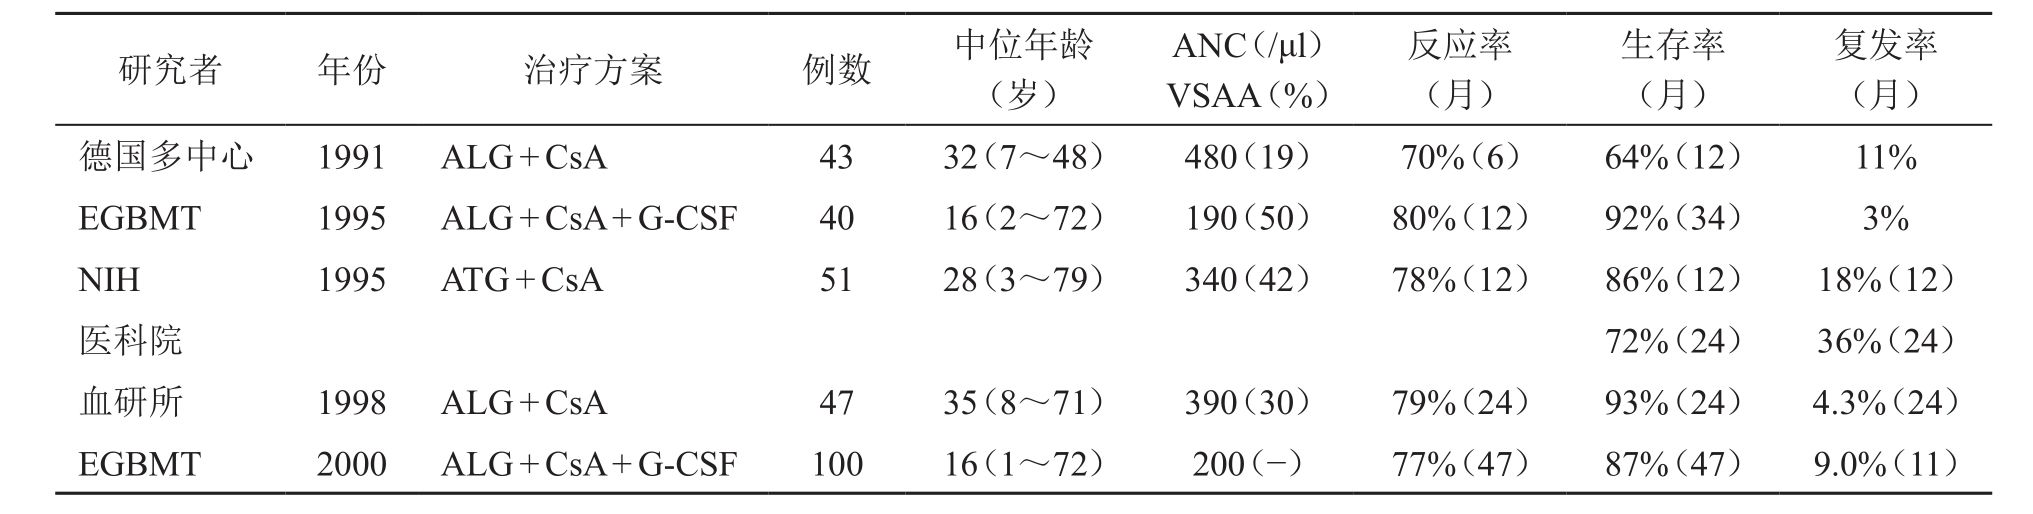
\includegraphics[width=6.77083in,height=1.70833in]{./images/Image00128.jpg}
\end{table}

近年来Allo-BMT及免疫抑制疗法已成为SAA两大标准疗法。Allo-BMT不仅疗效佳,且长期生存者可被认为已获“治愈”,但无效者极难恢复自身造血功能,治疗相关性死亡率仍较高;20世纪90年代以来随着免疫抑制疗法疗效进一步提高,目前免疫抑制疗法疗效与Allo-BMT具有可比性,且治疗相关性死亡率较低。大量结果显示,Allo-BMT疗效与患者年龄有关:<
20岁患者(尤其是VSAA患者)疗效最佳;>
40岁患者疗效最差,故对40岁以上及40岁以下无Allo-BMT条件患者可首选免疫抑制疗法。UCLA比较了同期同一年龄组(16~43岁)接受ATG(56例)及Allo-BMT(55例)治疗SAA患者的疗效,6年生存率分别为49\%
± 4\%及52\% ± 7\%,两者相比,无显著性差异(P =
0.8)。对于20~40岁患者,选择何种治疗方案更为适宜,存在两种截然相反观点:有些学者主张凡是年龄≤55岁,并有HLA匹配同胞体供患者均首选Allo-BMT;相当一部分学者认为免疫抑制疗法与Allo-BMT疗效具有可比性,首选免疫抑制疗法更为适宜。

\begin{figure}[!htbp]
 \centering
 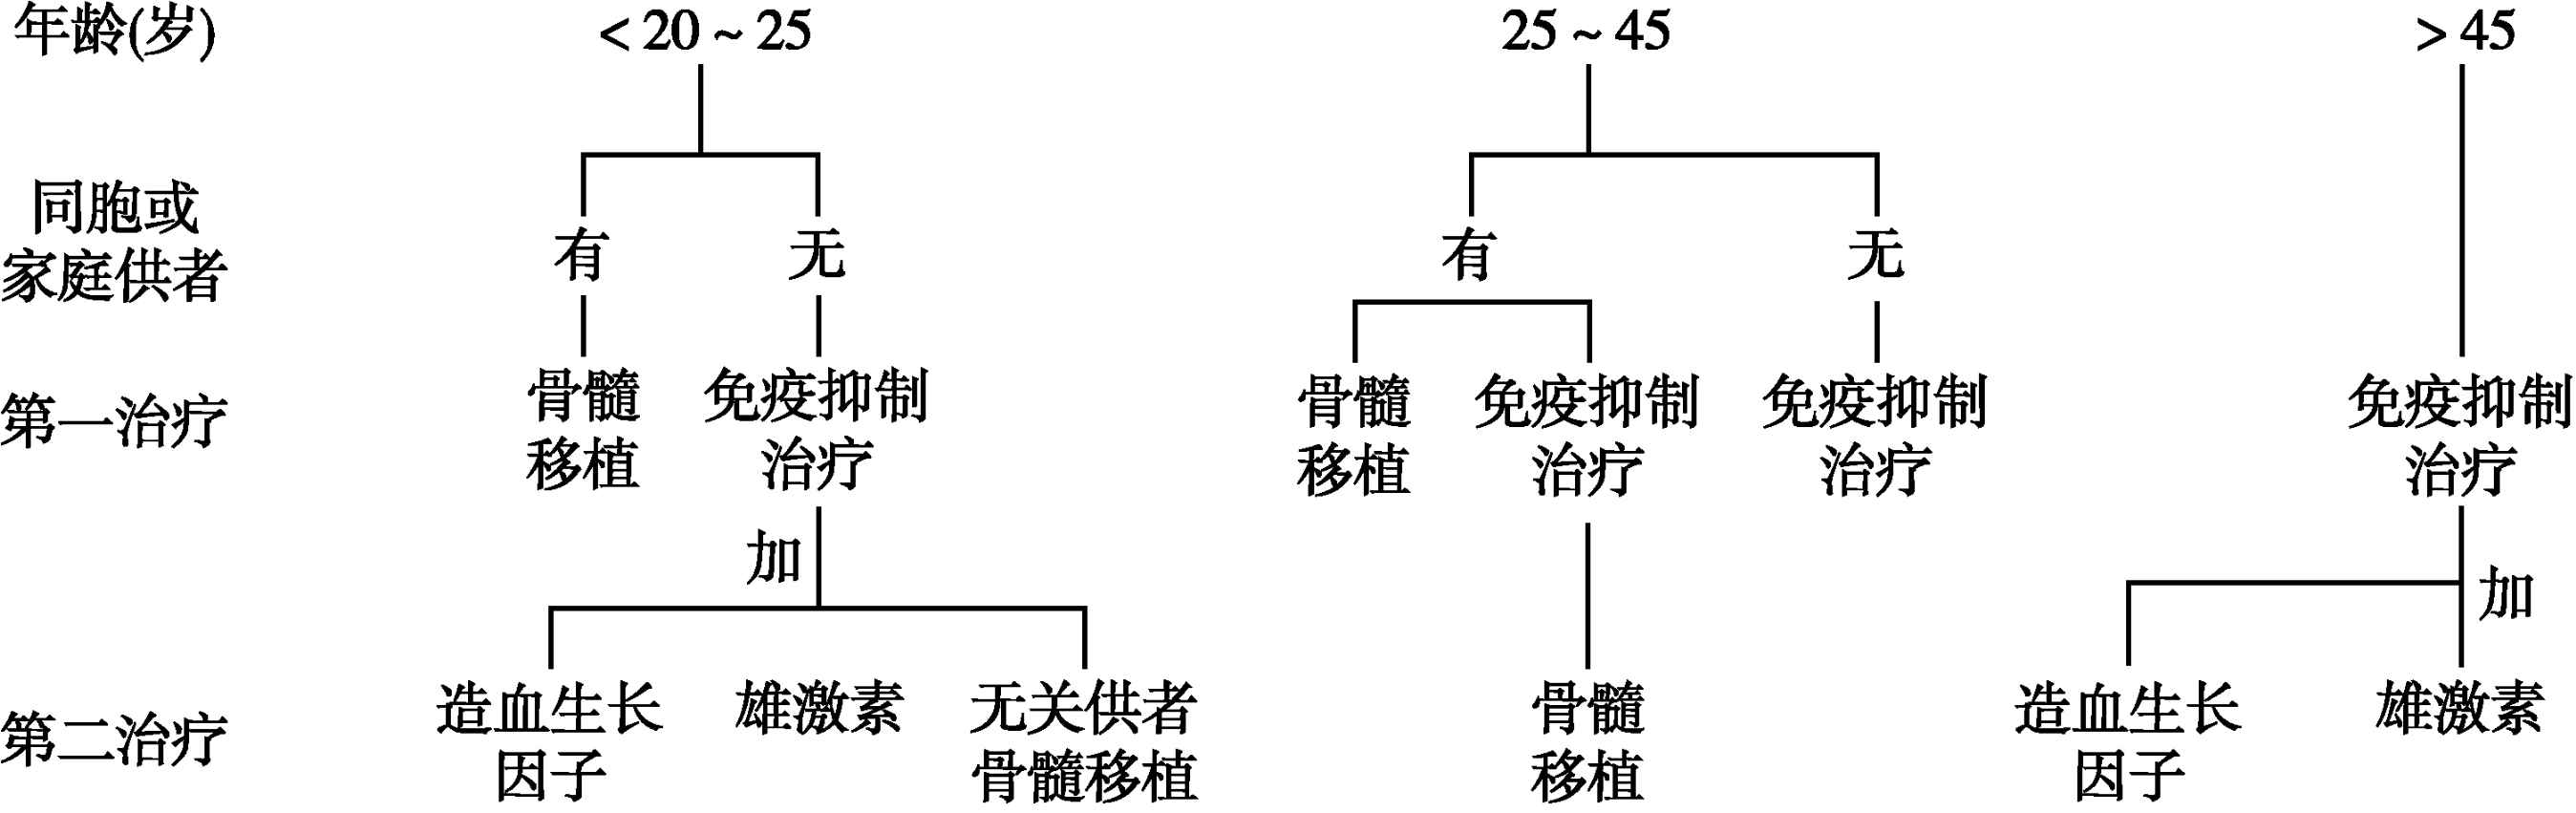
\includegraphics[width=5.01042in,height=1.58333in]{./images/Image00129.jpg}
 \captionsetup{justification=centering}
 \caption{SAA Allo-BMT或免疫抑制治疗的选择}
 \label{fig34-1}
  \end{figure} 

前已述及,既往一般认为对于年龄<
20岁的SAA患者,Allo-BMT疗效显著优于免疫抑制疗法,但最近Lawlor等对一组年龄小于17岁的27例儿童SAA进行了长期随访,Allo-BMT(9例)及免疫抑制疗法组(18例)长期实际生存率分别为75\%及92\%,作者认为免疫抑制疗法可以作为儿童SAA的首选治疗手段。总之,国内外学者对此还未达成共识。参考Young意见,SAA患者在选择治疗方案时一般遵循以下程序(图\ref{fig34-1})。

\protect\hypertarget{text00090.html}{}{}

\section{再生障碍危象}

再生障碍危象(aplastic
crisis)是指慢性溶血过程中,由于某些病因突然导致骨髓造血功能障碍,临床表现为贫血突然加重,并可有不同程度的白细胞及血小板减少。

现在已知,再生障碍危象可见于多种慢性遗传性溶血性疾患,如遗传性球形红细胞增多症(HS)、镰状细胞贫血、丙酮酸激酶缺乏症等。还可见于获得性溶血性疾患如自身免疫性溶血性贫血(AIHA)、PNH;也可见于非溶血性疾患,如缺铁性贫血(IDA)、淋巴瘤等,还可见于非血液系统疾病。

\subsection{病因与发病机制}

患者发生再生障碍危象前常先有短暂上呼吸道感染或胃肠炎。此外本病有时也可发生于非典型肺炎、腮腺炎和传染性单核细胞增多症患者,故认为感染,尤其是病毒感染可能是本病的主要原因。有些药物也能引起再生障碍危象,如氯霉素、苯妥英钠、磺胺类药物、秋水仙碱等,提示这些药物抑制了DNA合成从而引起再生障碍危象。

\subsection{诊断}

慢性溶血性贫血患者突然发生贫血及乏力加剧,则应考虑到再生障碍危象。有些患者先有上呼吸道感染或消化道感染的症状,感染症状一般较轻,但也有体温>
40℃以上者,有些患者可因血小板减少而发生出血倾向,有些患者无任何先兆,如非血液病患者发生再生障碍危象,其症状主要由原发病决定。

体格检查除发现皮肤苍白外,无显著的阳性体征。有些慢性溶血性贫血合并本病时,也可能看到黄疸减轻或消退。实验室检查发现贫血,红细胞形态的变化由原发疾病所决定,周围血网织红细胞缺如。血清胆红素正常或降低,可伴有不同程度白细胞及血小板减少。骨髓象可有两种表现:①红系统受抑制,有核红细胞甚少;②骨髓增生活跃,但红系细胞停滞于幼稚细胞阶段。骨髓中粒系也以成熟型为主,中幼粒细胞以上各阶段甚少见,严重感染时,胞浆中可出现空泡及中毒颗粒;巨核细胞数量减少,成熟巨核细胞增多,多无血小板形成,有退行性变化。

\subsection{治疗}

本病预后良好,多数患者可于1~2周内自行恢复。治疗目的在于帮助患者度过急性期。如贫血严重,以致发生症状时可适当输血;对继发性感染给以适宜抗生素治疗。如果病情严重,可给予刺激造血药物如造血细胞生长因子等,其他支持疗法包括给予多种维生素;注意补充叶酸;发热期间注意水电解质平衡。

\protect\hypertarget{text00091.html}{}{}

\hypertarget{text00091.htmlux5cux23CHP3-10-3}{}
参 考 文 献

1. Pulsipher MA,Young NS,Tolar J,et al. Optimization of therapy for
severe aplastic anemia based on clinical,biologic,and treatment
response parameters:conclusions of an international working group on
severe aplastic anemia convened by the blood and marrow transplant
clinical trials network,march 2010. Biol Blood Marrow
Transplant,2011,17(3):291-299

2. Li Y,Li X,Ge M,et al. Long-term follow-up of clonal evolutions in
802 aplastic anemia patients:a single-center experience. Ann
Hematol,2011,90(5):529-537

3. Marsh JCW,Ball SE,Cavenagh J,et al. Guidelines for the diagnosis
and management of acquired aplastic anaemia. Br J
Haematol,2009,147(1):43-70

4. Ades L,Mary JY,Robin M,et al. Long-term outcome after bone marrow
transplantation for severe aplastic anemia. Blood,2004,103:2490-2497

5. Brodsky RA,Jones RJ. Aplastic anaemia. Lancet,2005,365
(9471):1647-1656

\protect\hypertarget{text00092.html}{}{}

\chapter{多器官功能障碍综合征}

\section{概  论}

当机体受到严重感染、创伤、烧伤等严重打击后,2个或2个以上器官发生序贯性功能衰竭,称为多器官功能衰竭(multiple
organ failure,MOF)或多器官功能衰竭综合征(multiple organ failure
syndrome,MOFS)。

多器官功能障碍综合征(multiple organ dysfunction
syndrome,MODS)是1992年提出的概念,指各种疾病导致机体内环境稳态的失衡,包括早期多器官功能不全到多器官功能衰竭的全过程,是一个对MOF认识更早、范畴更广的概念。目前MOF病死率仍高达60\%~94\%,是严重感染、创伤和大手术后最常见的病死原因。

MOF是MODS的终末阶段。以MODS的概念代替MOF,反映了人们对多器官功能衰竭更为深入的认识和了解,将MODS定义为一个包括早期病理生理改变到终末期器官功能衰竭的连续的完整的病理生理过程,确立了动态和开放的MODS概念,为MODS的早期认识、早期诊断以及早期干预奠定了基础,具有重要的临床意义。

MODS概念的提出是对MOF认识进步的结果,但确定较为合理的MODS定义仍然困难。为了避免割裂MODS整个病理生理过程,美国胸科医师学会/美国危重病医学会提出了一个较为模糊的MODS定义,即各种疾病导致多个器官不能维持自身功能,从而影响全身内环境稳定性的状态。MODS表述的器官功能障碍可以是相对的,也可以是绝对的,而且器官功能障碍是动态的、连续的变化过程,对器官功能的动态观察必将有助于MODS的早期诊断和治疗。MODS是当前重症医学所面临的最大挑战。

\subsubsection{MOF前时代及历史回顾}

疾病的发生、发展和转归犹如一条长链,包含着许多环节,其中必然存在某些相对薄弱的环节,链条的强度由最薄弱的那个环节决定(a
chain is only as strong as its weakest
link),并不取决于最强的环节。最薄弱的环节将最先发生断裂,在疾病过程中,功能最为脆弱的器官将最早发生衰竭,这一现象在MOF提出之前尤为突出。

在MOF提出之前,临床医学、特别是外科学面临的难题主要是单一器官衰竭。某一器官衰竭可能危及患者生命,单器官衰竭是临床医师关注的焦点。近代战争对临床医学的影响不可低估。第二次世界大战期间及二战前,机体链条中最薄弱环节是循环,休克是当时最为突出的问题。随着对休克认识的进步,朝鲜战争期间,肾脏成为最薄弱的环节,急性肾衰竭是威胁患者生命的难题。而到20世纪60年代末的越南战争期间,机体最薄弱的环节转到肺,急性呼吸衰竭是危重患者死亡的主要原因。人类对疾病认识的进步,使机体最薄弱最容易断裂的环节不断发生改变。20世纪70年代前危重患者发生器官衰竭的最显著特点几乎均为单一器官衰竭,也就是说,由于缺乏有力的支持手段,一旦发生某一器官衰竭,患者往往死于该器官的衰竭。20世纪70年代以后,器官支持技术的进步,越来越多重症患者不再死于单一器官衰竭,而是死于多个器官衰竭。可以说,20世纪70年代以前实际上是“单器官衰竭时代”或“前MOF时代”。

\hypertarget{text00092.htmlux5cux23CHP3-11-1-1-1}{}
(一) 薄弱环节之一------休克

休克是二战及二战前危及危重患者生命的主要薄弱环节。在第一次世界大战期间,认识的贫乏,导致对创伤性休克的无知。血压的下降被认为是血管动力耗竭、肾上腺皮质功能衰竭和创伤毒素的结果,忽视了创伤后出血、脂肪栓塞和脑创伤等在休克中所起的关键作用。直到1930~1934年,Persons和Alfred
Balock等学者通过动物试验,证实并提出创伤性休克是血管内容量大量丢失的结果。尽管如此,第二次世界大战早期,多数学者依然认为创伤性休克是不可逆的,而且主要通过补充血浆恢复血容量、输注盐水纠正脱水和电解质的丢失。血液的丢失和输血未能得到应有的重视,大批创伤性休克士兵得不到积极有效的治疗。1943年美国哈佛大学外科学教授Churchill在纽约时报上撰文,指出严重创伤性休克患者存在大量血液丢失,单纯输注血浆和盐水是远不够的,必须输注全血。Churchill的呼吁引起强烈反响,美军在北非和意大利战场的前线战地医院,开始装备冰箱以贮存血液。早期积极输血、输液以恢复血容量、补充丢失的全血,大批创伤性休克患者奇迹般地获得存活,创伤性休克不可逆的观念被推翻。令人遗憾的是,部分创伤性休克患者在休克纠正后10天左右,出现无尿,进而死于急性肾衰竭。看来肾脏成为新的、容易发生断裂的机体链条的薄弱环节。

\hypertarget{text00092.htmlux5cux23CHP3-11-1-1-2}{}
(二) 薄弱环节之二------急性肾衰竭

对休克认识的偏差,导致肾脏成为机体链条的薄弱环节,临床医学的热点由休克转向急性肾衰竭。第二次世界大战后期及战后,人们对休克展开进一步研究,发现机体受到创伤打击后,醛固酮释放增加,导致钠潴留,而钾不受影响,仍然大量从肾脏排泄。醛固酮释放增加导致的水钠潴留本来是机体对有效循环血量减少而产生的代偿性反应。可惜认识的局限性,导致治疗的偏差,提出对创伤性休克患者应补充必要的全血、血浆,但限制盐水的输注,使机体处于液体偏少或“偏干”的状态,结果导致患者仍然处于低血容量状态。同时,由于把休克与血压低等同起来,认为只要血压正常休克即被纠正,形成以纠正血压为终点的休克治疗思想,使休克不能获得根本纠正,机体始终处于低血容量状态,急性肾衰竭的发生成为必然。

美军外科研究中心的报告显示,朝鲜战争期间,部分创伤性休克士兵经早期清创和血压纠正后,发生急性肾衰竭。200例严重创伤士兵中,就有1例发生急性肾衰竭,患病率是越南战争的20~30倍,而且一旦发生急性肾衰竭,病死率高达90\%。针对这一突出问题,美军外科研究中心提出了“创伤后急性肾脏功能衰竭”的观念,以期引起重视。Shires等学者很快认识到休克液体复苏不足和限制水钠摄入,导致细胞外液和血管内容量不足,是引起急性肾衰竭的主要原因。从而形成创伤性休克治疗的新思路,采取快速输血、输液等积极液体复苏手段,补足血管内容量和细胞外容量,在纠正循环衰竭的同时,早期恢复患者尿量,能够有效地防止急性肾衰竭。

\hypertarget{text00092.htmlux5cux23CHP3-11-1-1-3}{}
(三) 薄弱环节之三------急性呼吸衰竭

当创伤患者的循环和肾脏功能得到有效支持后,急性呼吸衰竭浮出水面,肺成为机体链条中最薄弱的环节。20世纪60年代末的越南战争期间,肺成为机体最突出的薄弱环节,急性呼吸衰竭是创伤危重患者死亡的主要原因,病死率高达92\%。针对急性呼吸衰竭在创伤中的重要地位,提出了“创伤后急性呼吸衰竭”的观念。早期大量、甚至过量的液体复苏对纠正休克和防止肾衰是有利的,急性肾衰竭的发生率降低到0.1\%~0.2\%,仅为朝鲜战争的1/5~1/2,但过高的液体负荷损伤肺脏,加上创伤对肺的直接打击,急性呼吸衰竭在所难免。呼吸支持技术和适当的容量管理成为急性呼吸衰竭治疗的关键。

\subsubsection{MOF概念的提出------MOF时代}

当全力支持机体链条中某一薄弱环节时,如造成链条薄弱的因素依然存在,则其他隐性、潜在的薄弱环节还可能发生断裂,而且形成序贯性的断裂。多个薄弱环节或多个断裂同时存在,将使处理变得复杂,而且难以修复。这正是MOF的形象比喻。

20世纪70年代以来
,我们进入“MOF时代”。器官支持技术的进步,使越来越多重症患者不再是发生单一器官衰竭,而是多个器官衰竭。20世纪70年代初,急性肾衰竭的发生率明显降低,但引起急性肾衰竭的原发病------感染或创伤,进一步导致休克或肝脏功能衰竭。通过血液透析替代肾脏功能,使多数患者并不死于急性肾衰竭,却死于休克和肝衰竭,病死率仍高达63\%~77\%。严重创伤或感染后,重症患者胃肠道蠕动消失,实际上也是一种类型的肠道功能衰竭,导致肠道毒素或细菌移位、出血或穿孔等严重后果。同样,创伤或感染后,患者出现肝肿大和黄疸,则提示发生急性肝功能衰竭。最近代谢衰竭和“自噬现象”也日益受到重视。机体任何器官和系统均可能发生衰竭(表\ref{tab35-1}),但是否同时发生或是序贯性的发生,则取决于机体的状态、损伤的严重程度和并发症的发展情况。

\begin{table}[htbp]
\centering
\caption{多器官功能衰竭可累及的器官或系统}
\label{tab35-1}
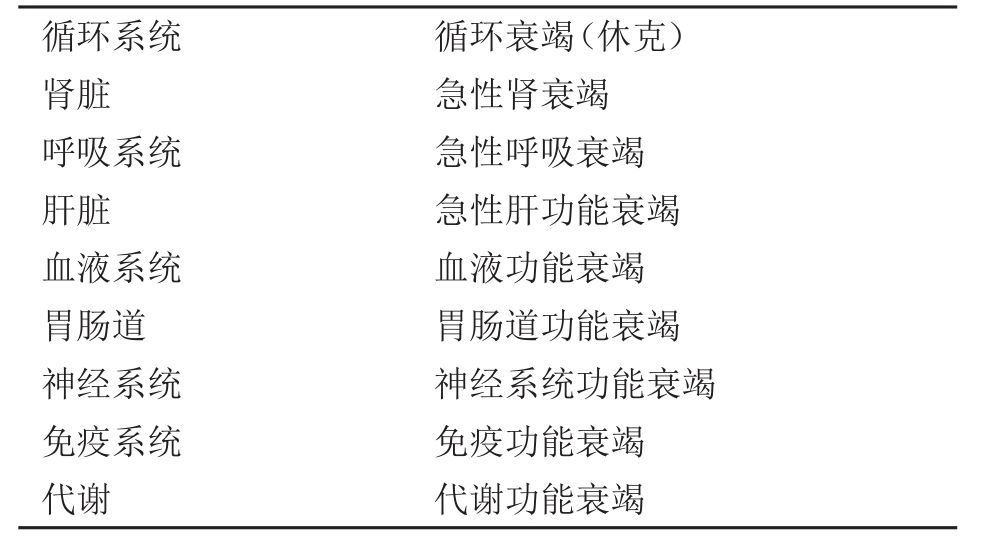
\includegraphics[width=3.3125in,height=1.83333in]{./images/Image00130.jpg}
\end{table}

1973年
Tilney首先提出了“序贯性器官功能衰竭”的概念。作者观察了18例腹主动脉瘤术后并发急性肾衰竭的患者,尽管给予积极治疗,均先后出现急性肺水肿(非心源性)、急性胰腺炎和急性肾衰竭等序贯性功能衰竭,病死率高达94\%。作者认为腹主动脉瘤手术创伤导致患者发生多个器官的序贯性衰竭,并指出相继衰竭的器官可以是远隔器官,而并不一定是最初受损的器官。“序贯性器官功能衰竭”的提出是MOF研究的一个里程碑,为临床医师重视MOF奠定了基础。

1975年
Baue进一步提出了序贯性器官功能衰竭综合征,首次将MOF概括为一综合征。3例患者的原发性疾病并不相同,但最终均发生MOF而死亡,尸检显示类似的结果。第1例为结肠切除患者,术后发生吻合口瘘和急性腹膜炎,在积极治疗6周后死亡。尸检显示肺充血水肿、局灶性肺纤维化和肺炎、急性肾小管坏死伴肾小球内血栓形成、急性非炎症性肝坏死、脾脏多发性梗死、肾上腺自溶。可以看出,尽管患者死于急性腹膜炎,但受累器官包括腹腔内的肝脏、腹膜后的肾脏和肾上腺及腹腔外的肺脏。第2例原发疾病为急性重症胰腺炎,尸检显示全身黄疸、胸腔积液、吸入性肺炎、急性肾小管坏死、肝脏弥漫性坏死、胃肠道溃疡。同样显示了原发病灶胰腺以外的多个器官发生衰竭。而第3例患者为二尖瓣和主动脉瓣置换术后伴持续低心排,积极治疗一个半月后死亡,尸检发现细菌性坏死性动脉炎、间质性肺水肿伴透明膜形成、急性肝脏小叶中央型坏死、急性肾衰竭和脾脏淤血。从3例患者的原发疾病和尸检情况可以看出,原发疾病尽管不同,但最终均发展为MOF,而且受累的衰竭器官可以是原发病灶邻近器官,也可以是远隔器官。由于不同原发疾病导致了类似的多个器官相继发生功能衰竭,Baue将其归纳为一个综合征“多系统进行性序贯性器官功能衰竭(multiple
progressive or sequential system
failure)”,并指出当单一器官功能衰竭被征服或功能被替代后,多器官的衰竭正在成为一种新的威胁,一个令人不安的新时代(MOF时代)已经来临。

1977年
Polk针对MOF多发生于原发部位远隔器官,提出“远隔器官功能衰竭”,但未被广泛采用。同年Eiseman将不同原发疾病导致的多个器官相继发生功能衰竭这一综合征命名为“multiple
organ
failure”(MOF),这一术语简单明了,迅速被推广采用,至今依然沿用。应该指出,多器官功能衰竭不是单纯的一种综合征,而是作为一个新的概念被提出来的。

\begin{table}[htbp]
\centering
\caption{多器官功能衰竭及多器官功能障碍综合征的名称}
\label{tab35-2}
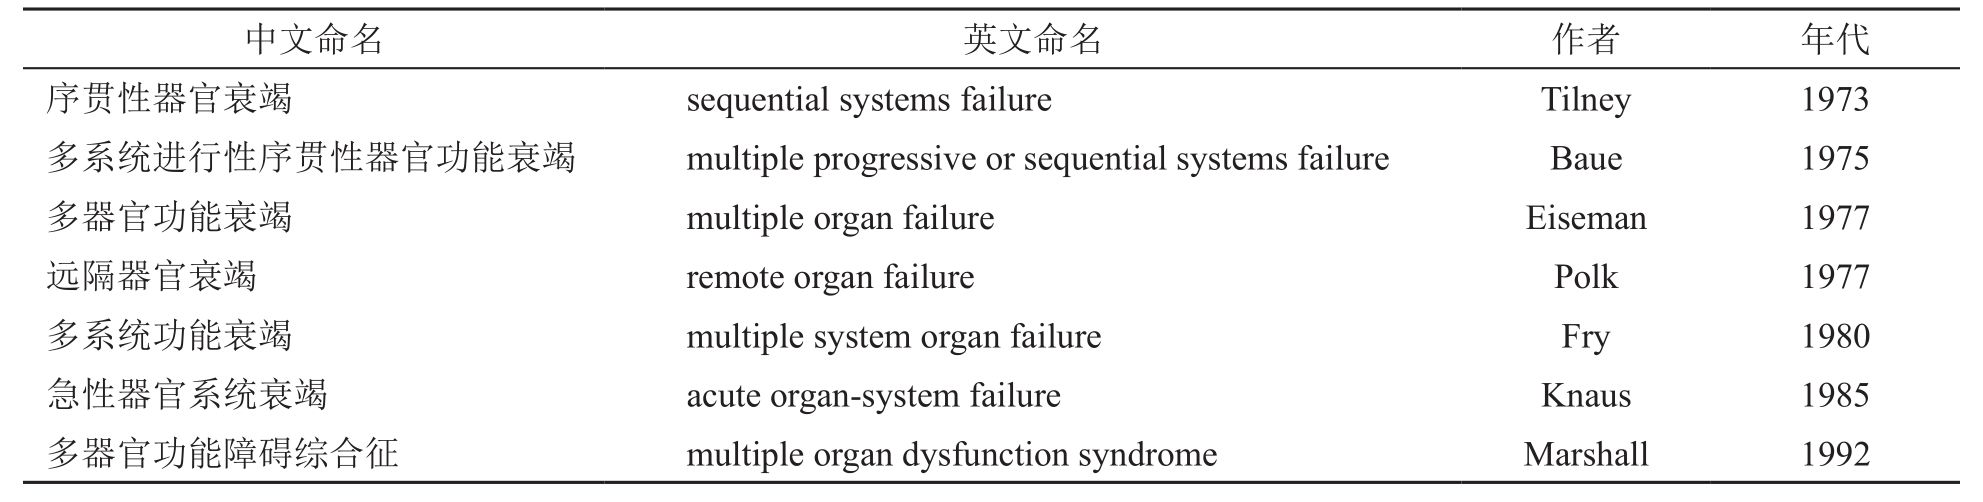
\includegraphics[width=6.60417in,height=1.66667in]{./images/Image00131.jpg}
\end{table}

MOF曾被冠以许多名称(表\ref{tab35-2}),但MOF这一术语被普遍接受和使用。直到1992年,美国胸科医师学会/重症医学会(ACCP/SCCM)提出以多器官功能障碍综合征(multiple
organ dysfunction
syndrome,MODS)代替MOF。MODS是各种疾病导致机体内环境稳态失衡的状态。目前认为MODS实际上就是全身性炎症反应失控引起的多器官功能障碍。因此,MODS也可理解为全身性炎症反应综合征+器官功能障碍,而传统的MOF就是MODS继续发展的最严重的终末期结果。

以MODS代替MOF反映了人们对该综合征更为深入的认识和了解,具有重要的临床意义。第一,MODS是一个包括早期内环境紊乱到MOF的连续的病理生理过程,而不是一个孤立事件,具有较宽的内涵。第二,MODS的提出也是对MOF痛苦反思的结果,当患者诊断MOF时,器官功能衰竭已到晚期,常常痛失治疗时机。对多器官功能衰竭的早期干预,前提是对MOF的早期认识。MODS的提出为早期认识、早期诊断以及早期干预奠定了基础。

\protect\hypertarget{text00093.html}{}{}

\section{炎症反应与多器官功能障碍综合征病理生理机制}

多器官功能障碍综合征(MODS)的发病机制非常复杂。以往认为MODS是感染、创伤、烧伤等严重机体损伤难以遏制的直接后果。近20年的研究涉及了MODS的病理生理学、病理学、免疫学、分子生物学以及分子流行病学,对MODS的认识逐步深刻。目前认为,MODS不仅与感染、创伤等直接损伤有关。在某种程度上,MODS与机体自身对感染、创伤的免疫炎症反应具有更为本质性的联系。也就是说MODS的最大的威胁来自失控的炎症反应。对机体炎症反应的深刻认识有利于早期认识MODS病理生理紊乱,并使早期积极干预成为可能。MODS发病机制提出了不少学说,但归纳起来主要包括炎症反应学说、自由基学说和肠道动力学说。

\subsubsection{MODS的传统认识}

传统观念认为多器官功能衰竭(MOF)/MODS是严重感染或创伤的直接后果,也就是说入侵的细菌/内毒素或组织损伤是导致MODS的根本原因。随着研究的深入,对MODS的认识也逐渐变化。1973年Tilney首先撰文描述了多器官功能序贯性衰竭,并指出相继衰竭的器官可以是远隔器官,而并不一定是最初受损的器官。1977年Polk认为远隔器官的功能衰竭是隐匿性腹腔感染的结果。1980
年Fry进一步提出革兰阴性杆菌是导致MOF的最常见原因。受上述理论的影响,对于MOF的诊疗,临床上积极使用抗生素,并致力于寻找隐匿的感染灶,甚至在缺乏充分证据的情况下,主张经验性治疗或早期剖腹探查,以期发现隐匿的或未控制的感染灶,达到控制感染、防治MOF的目的。遗憾的是,积极的治疗并未获得预期疗效。

创伤感染是否是导致MODS的根本原因,值得怀疑。1985年Norton观察了21例腹腔脓肿患者,经多次积极的腹腔引流和抗生素治疗,仍有16例死于MODS。他认为即使充分的脓肿引流和抗生素治疗,并不能使MODS逆转,也不能降低病死率。之后,又有研究发现死于MOF的菌血症患者中,在剖腹探查或尸检中,有30\%无感染灶发现。在此基础上,1985年Goris指出,MODS并非细菌/毒素或组织损伤直接作用的后果,可能是机体炎症反应紊乱的结果。这是MODS认识上的重大飞跃。根据一系列的实验和临床观察,形成MODS的理论假设,即机体在遭受细菌或毒素打击时,炎症细胞大量激活和炎症介质异常过量释放,并涌入循环产生持续性全身性炎症瀑布反应,这是导致MODS的根本原因。换句话说,感染或组织损伤导致机体炎症反应失控,造成广泛自身组织破坏,最终导致MODS,甚至死亡。

\subsubsection{MODS的发病机制}

正常情况下,感染和组织创伤时,局部炎症反应对细菌清除和损伤组织修复都是必要的,具有保护性作用。当炎症反应异常放大或失控时,炎症反应对机体的作用从保护性转变为损害性,导致自身组织细胞死亡和器官衰竭。无论是感染性疾病(如严重感染、重症肺炎、急性重症胰腺炎后期),还是非感染性疾病(如创伤、烧伤、休克、急性胰腺炎早期等)均可能导致MODS。可见,任何能够导致机体免疫炎症反应紊乱的疾病均可引起MODS。从本质上来看,MODS是机体炎症反应失控(uncontrolled
inflammation)的结果。感染创伤是机体炎症反应的促发因素,而机体炎症反应的失控,最终导致机体自身性破坏,是MODS的根本原因(图\ref{fig35-1})。炎症细胞激活和炎症介质异常释放、组织缺氧和自由基、肠道屏障功能破坏和细菌/毒素移位均是机体炎症反应失控的表现,构成了MODS的炎症反应失控的3个互相重叠的发病机制学说------炎症反应学说、自由基学说和肠道动力学说(图\ref{fig35-2})。

\begin{figure}[!htbp]
 \centering
 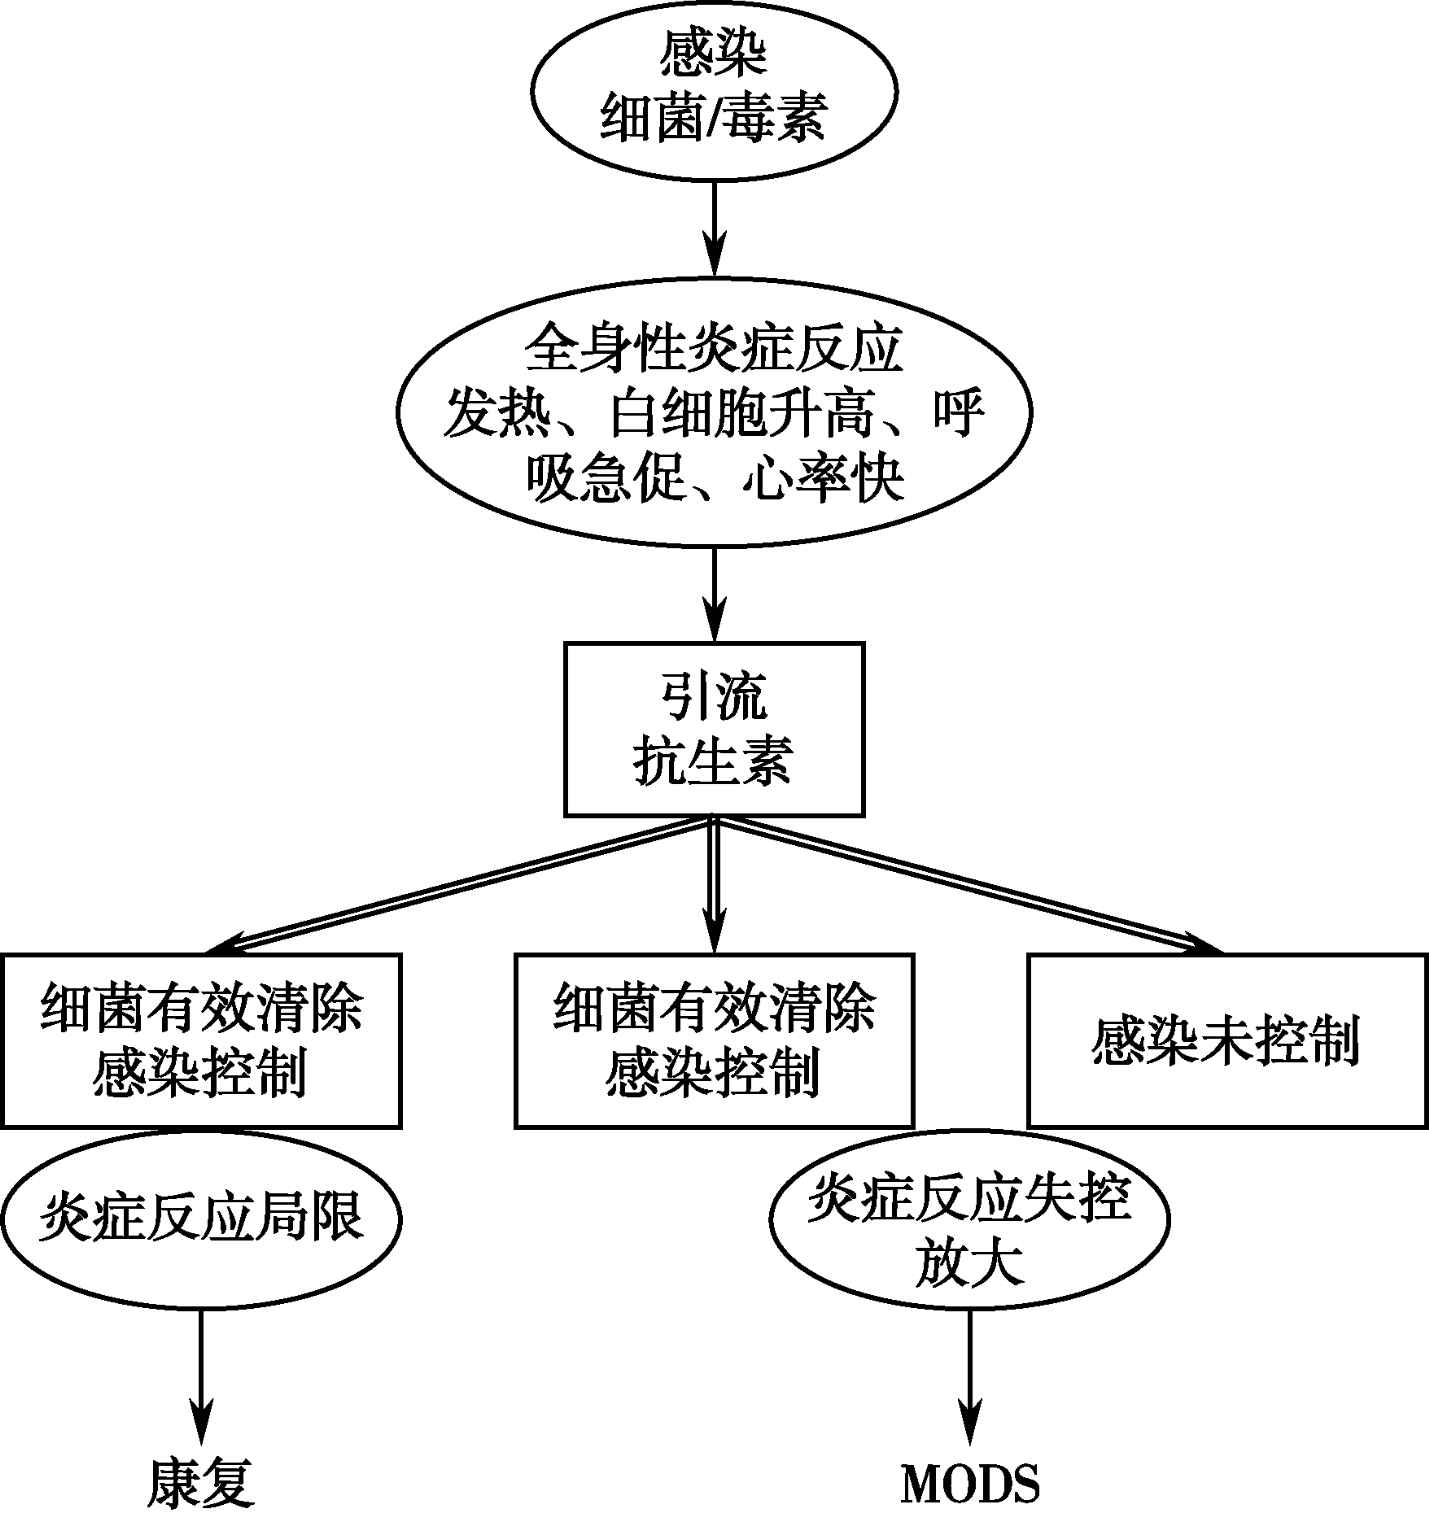
\includegraphics[width=2.91667in,height=3.10417in]{./images/Image00132.jpg}
 \captionsetup{justification=centering}
 \caption{多器官功能障碍综合征与炎症反应的关系}
 \label{fig35-1}
  \end{figure} 

\begin{figure}[!htbp]
 \centering
 
\includegraphics[width=2.85417in,height=1.32292in]{./images/Image00133.jpg}
 \captionsetup{justification=centering}
 \caption{多器官功能障碍综合征的发病机制}
 \label{fig35-2}
  \end{figure} 

\hypertarget{text00093.htmlux5cux23CHP3-11-2-2-1}{}
(一) 炎症反应学说

炎症反应学说是
MODS发病机制的基石,基本内容包括感染或创伤引起的毒素释放和组织损伤并不是导致器官功能衰竭的直接原因,细菌/毒素和组织损伤所诱发的全身性炎症反应是导致器官功能衰竭的根本原因。

当机体遭受感染或创伤打击后,细菌/毒素或组织损伤将刺激机体巨噬细胞等炎症细胞,释放炎症介质。肿瘤坏死因子是最早释放的炎症介质之一,可进一步刺激和激活巨噬细胞、粒细胞、淋巴细胞和内皮细胞,释放大量的炎症介质,形成炎症介质释放的瀑布样连锁反应,犹如多米诺骨牌逐级放大,形成失控的炎症反应。参与炎症反应的介质包括:①炎症性细胞因子:肿瘤坏死因子(TNF)α、白细胞介素(IL)-1β、IL-2、IL6、IL-8等;②自由基类介质:氧自由基、氮氧自由基等;③脂质代谢产物:白三烯、前列腺素、血小板活化因子等;④其他介质:溶酶体酶、缓激肽、组织胺、补体激活产物等。尽管一氧化氮和前列腺素被认为是炎症介质瀑布样反应的最后共同途径,导致血管麻痹和休克,但它们与其他炎症介质一起,均可引起组织细胞损害,最终导致MODS。

炎症反应学说在MODS发病机制中的根本性作用,得到大量实验和临床研究的证实:①内毒素血症导致的MODS模型动物及因感染、烧伤和创伤而发生MODS患者,血浆和局部组织(如肺泡灌洗液、脑脊液、腹水、胸水等)的炎症介质浓度明显升高,而且炎症介质的水平与疾病严重程度有一定关系;②给动物注射内毒素或炎症介质(如TNFα和IL-1β),不但可引起严重炎症反应,而且可进一步诱发MODS。给健康志愿者静脉注射小剂量内毒素和炎症介质也可导致明显的炎症反应;③注射单克隆抗体以阻断内毒素或炎症介质的效应,可防止感染动物发生MODS,降低病死率。

抑制或中和关键性炎症介质,阻断炎症反应的多米诺效应,寻找防止MODS的“魔弹”,一度成为MODS研究热点。动物实验显示早期给予单克隆抗体,阻断内毒素、TNFα、IL-1β、Il-6和干扰素(IFN)γ的作用,具有降低动物炎症反应和病死率的作用,结果令人鼓舞。然而,耗资巨大的小规模临床试验并未获得满意的临床结果,而且在某些感染的动物模型中,抑制或阻断一氧化氮反而加重肺损伤,产生有害的血流动力学影响。抗介质治疗战略的失败,使人们深刻反思MODS的炎症反应机制。①细胞因子等炎症介质的作用机制方面存在种族差异,动物试验的研究结果不能直接惠及人类。②免疫功能状态存在差异,接受静脉注射内毒素或细胞因子健康动物或志愿者的免疫功能状态,与创伤感染后动物或患者差异很大。给损伤后动物注射IFNγ,可降低致命性腹腔感染的病死率。同样剂量的IFNγ给未损伤的动物注射,之后再给动物注射内毒素,动物病死率明显增加,可见动物的免疫状态不同,对IFNγ的反应性也截然相反。③实验动物所接受的内毒素或细胞因子往往为一次性、攻击性的大剂量,而临床感染中,内毒素或细胞因子的释放往往为较小剂量、反复持久的。④细胞因子以旁分泌和自分泌为主,组织局部的细胞因子浓度往往很高,而循环中水平较低。但实验和临床抗介质治疗均以对抗血浆炎症介质为目标。⑤细胞因子等炎症介质实际上是一把“双刃剑”,在不同浓度、不同状态、不同组织部位,可能具有不同的作用,甚至作用是完全相反的。

尽管认识还不全面,但炎症反应失控依然是MODS发生、发展中的根本性作用,炎症反应学说依然是MODS发病机制的基石。

\hypertarget{text00093.htmlux5cux23CHP3-11-2-2-2}{}
(二) 自由基学说

缺血再灌注和自由基也是导致
MODS的重要机制之一。MODS的自由基学说主要包括3方面:①氧输送不足导致组织细胞直接的缺血缺氧性损害;②缺血再灌注促发自由基大量释放;③白细胞与内皮细胞的互相作用,导致组织和器官损伤,最终发生MODS。从根本上来看,自由基学说也是炎症反应学说的重要组成部分。

缺血缺氧引起组织器官损伤是MODS的重要原因。当氧输送低于临界水平时,必然引起全身组织器官的缺血缺氧,导致器官功能损害。以Shoemaker为代表的学者提出,通过提高心输出量、血红蛋白浓度或动脉血氧饱和度,使全身氧输送明显高于临界水平,即超常水平的氧输送(supernormal),可以达到改善组织器官缺氧的目的。尽管高氧输送是符合逻辑的,但全身氧输送的提高与某一器官血流和氧输送改变并不一致。当全身氧输送高于正常时,肠道、肝脏等内脏器官仍然可能处于缺血缺氧状态。研究证实,以提高氧输送为复苏目标,并不能改变MODS的预后。肠道是休克及MODS中最易发生缺血缺氧的器官,对肠道缺血的监测可能是有益的。肠道黏膜pH监测可判断肠道缺血程度,用以指导MODS患者的复苏治疗似乎更为合理,但以改善器官氧输送为目标的复苏治疗,是否能够最终改善MODS患者的预后,尚待进一步研究。

再灌注和自由基的释放也是导致MODS的重要机制。组织器官血流灌注的恢复或重建对于机体的生存是很有必要的,但却能诱导自由基的释放。黄嘌呤氧化酶和白细胞激活途径是自由基生成的主要来源。黄嘌呤脱氢酶转化为黄嘌呤氧化酶是自由基释放的前提,一般情况下,肠道再灌注10秒后,黄嘌呤脱氢酶即转化为黄嘌呤氧化酶;在心肌组织中,酶的转化发生于再灌注后8分钟左右;而在肝脏、脾脏、肾脏和肺等器官,酶的转化发生在再灌注后30分钟。再灌注后不同组织器官酶转化时间的差异,是不同组织器官缺血再灌注损伤程度不同的基础。再灌注和自由基造成的损害往往比缺血更为严重,因此,组织器官最严重的损伤不是发生在缺血期,而是发生在再灌注期。针对再灌注期自由基对组织细胞的严重损害,抑制自由基生成、阻断自由基作用或直接中和自由基,则成为合理的MODS防治战略。实验研究证实,应用自由基阻滞剂或清除剂可以保护器官功能,但对炎症反应和MODS的临床疗效不肯定。天然超氧化物歧化酶(SOD)在血浆中的半衰期很短,且难以通过细胞膜,单独应用不易发挥抗氧化作用。研制理想的抗氧化剂是阻断缺血再灌注损伤的希望。

由毒素和炎症介质诱导的失控炎症反应,在很大程度上作用于血管内皮细胞水平。正常情况下,内皮细胞表现为非炎症性表型,具有调节毛细血管血流、参与凝血和炎症反应的功能。当内毒素或炎症介质作用于内皮细胞时,内皮细胞可表达组织因子激活外源性凝血途径,表达表面受体(内皮细胞-粒细胞黏附分子ELAM、细胞间黏附分子ICAM-1等),促进白细胞与内皮细胞黏附和激活。此时毛细血管不再是炎症细胞的被动通道,而是炎症反应的积极参与者,促进炎症细胞向感染损伤部位趋化,激活炎症细胞,增强炎症细胞对细菌和异物的清除能力,有助于感染的控制和局限。但当局部炎症反应放大或失控时,毒素和炎症介质不仅刺激损伤部位的毛细血管内皮,而且可能弥漫性损伤全身毛细血管内皮细胞,结果造成微血栓形成及器官功能损害,导致MODS。可以说,感染创伤等各种因素诱导MODS的共同途径是内皮细胞的激活和白细胞与内皮细胞的黏附。以抑制白细胞与内皮细胞黏附为主要目标的内皮细胞保护性措施也是MODS的治疗策略之一,可减轻由休克或缺血再灌注介导的毛细血管内皮及组织器官损害,但也有可能抑制机体对致病菌的清除能力。内皮细胞保护策略有待进一步研究证实。

\hypertarget{text00093.htmlux5cux23CHP3-11-2-2-3}{}
(三) 肠道动力学说

肠道动力学说的概念最早是由
Meakins和Marshall提出的。1985年Goris对MODS患者的研究显示,死于MODS的患者中,30\%血培养阳性或有全身性感染的表现,但找不到感染灶。肠道是机体最大的细菌和毒素库,肠道有可能是MODS患者菌血症的来源。另外MODS患者菌血症的细菌往往与肠道菌群一致。因此,Meakins和Marshall提出肠道可能是MODS发生发展的动力器官(gut
motor)。

目前,肠道动力学说已被基本证实,临床和实验研究证据包括:①约1/3的菌血症患者死于MODS而未发现明确的感染灶;②肠道对缺血和再灌注损伤最为敏感,创伤或感染患者或动物模型中,细菌或毒素移位已被证实;③应用肠道营养,保持肠黏膜的完整性,可降低感染发生率。但对这一学说也有不同的看法:①休克或创伤后,肠黏膜通透性增加与感染并发症并无必然联系;②细菌可从肠系膜淋巴结中检出,但进入循环很少;③选择性肠道去污染(SDD)对降低肺部感染有益,但对MODS的发病和病死无明显影响。

根据目前的认识水平,肠道不仅仅是一个消化器官,由于肠黏膜内大量散在分布的淋巴细胞、肠系膜中广泛分布的淋巴结以及肝脏内大量的库普弗细胞,肠道实际上也是一个免疫器官。在感染、创伤或休克时,即使没有细菌的移位,肠道内毒素的移位也将激活肠道及其相关的免疫炎症细胞,导致大量炎症介质的释放,参与MODS的发病。因此,肠道是炎症细胞激活、炎症介质释放的重要场地之一,也是炎症反应失控的策源地之一。从这一点来看,肠道动力学说实际上是炎症反应学说的一部分。

\subsubsection{二次打击学说与MODS}

MODS往往是多元性和序贯性损伤的结果,而不是单一打击的结果。1985年Dietch提出MODS的二次打击学说,将创伤、感染、烧伤、休克等早期直接损伤作为第一次打击,第一次打击所造成的组织器官损伤是轻微的,虽不足以引起明显的临床症状,但最为重要的是,早期损伤激活了机体免疫系统,尽管炎症反应的程度较轻,但炎症细胞已经被动员起来,处于预激活状态。此后,如病情稳定,则炎症反应逐渐缓解,损伤组织得以修复。当病情进展恶化或继发感染、休克等情况,则构成第二次或第三次打击。第二次打击使已处于预激活状态的机体免疫系统暴发性激活,大量炎症细胞活化、炎症介质释放,结果炎症反应失控,导致组织器官的致命性损害。第二次打击强度本身可能不如第一次打击,但导致炎症反应的暴发性激活,往往是致命性的(图\ref{fig35-3})。

当第一打击强度足够大时,可直接强烈激活机体炎症反应,导致MODS,属于原发性MODS。但大多数患者MODS是多元性和序贯性损伤的结果,并不是单一打击的结果,这类MODS属于继发性MODS。常见的第二次打击包括继发性感染、休克、缺氧、缺血、创伤、手术等。对于多发性创伤的患者,如创伤严重,则直接可导致MODS。但多数患者经早期清创处理后基本稳定,而创伤早期发生的低血压导致各器官发生不同程度的缺血再灌注损伤及巨噬细胞、中性粒细胞激活,使患者出现发热、白细胞升高等炎症反应表现。创伤后3~7天,继发性感染或休克,使已处于预激活或激活状态的炎症细胞发生暴发性激活,结果使炎症反应失控,导致自身组织器官的损害,最终发展为MODS。

\begin{figure}[!htbp]
 \centering
 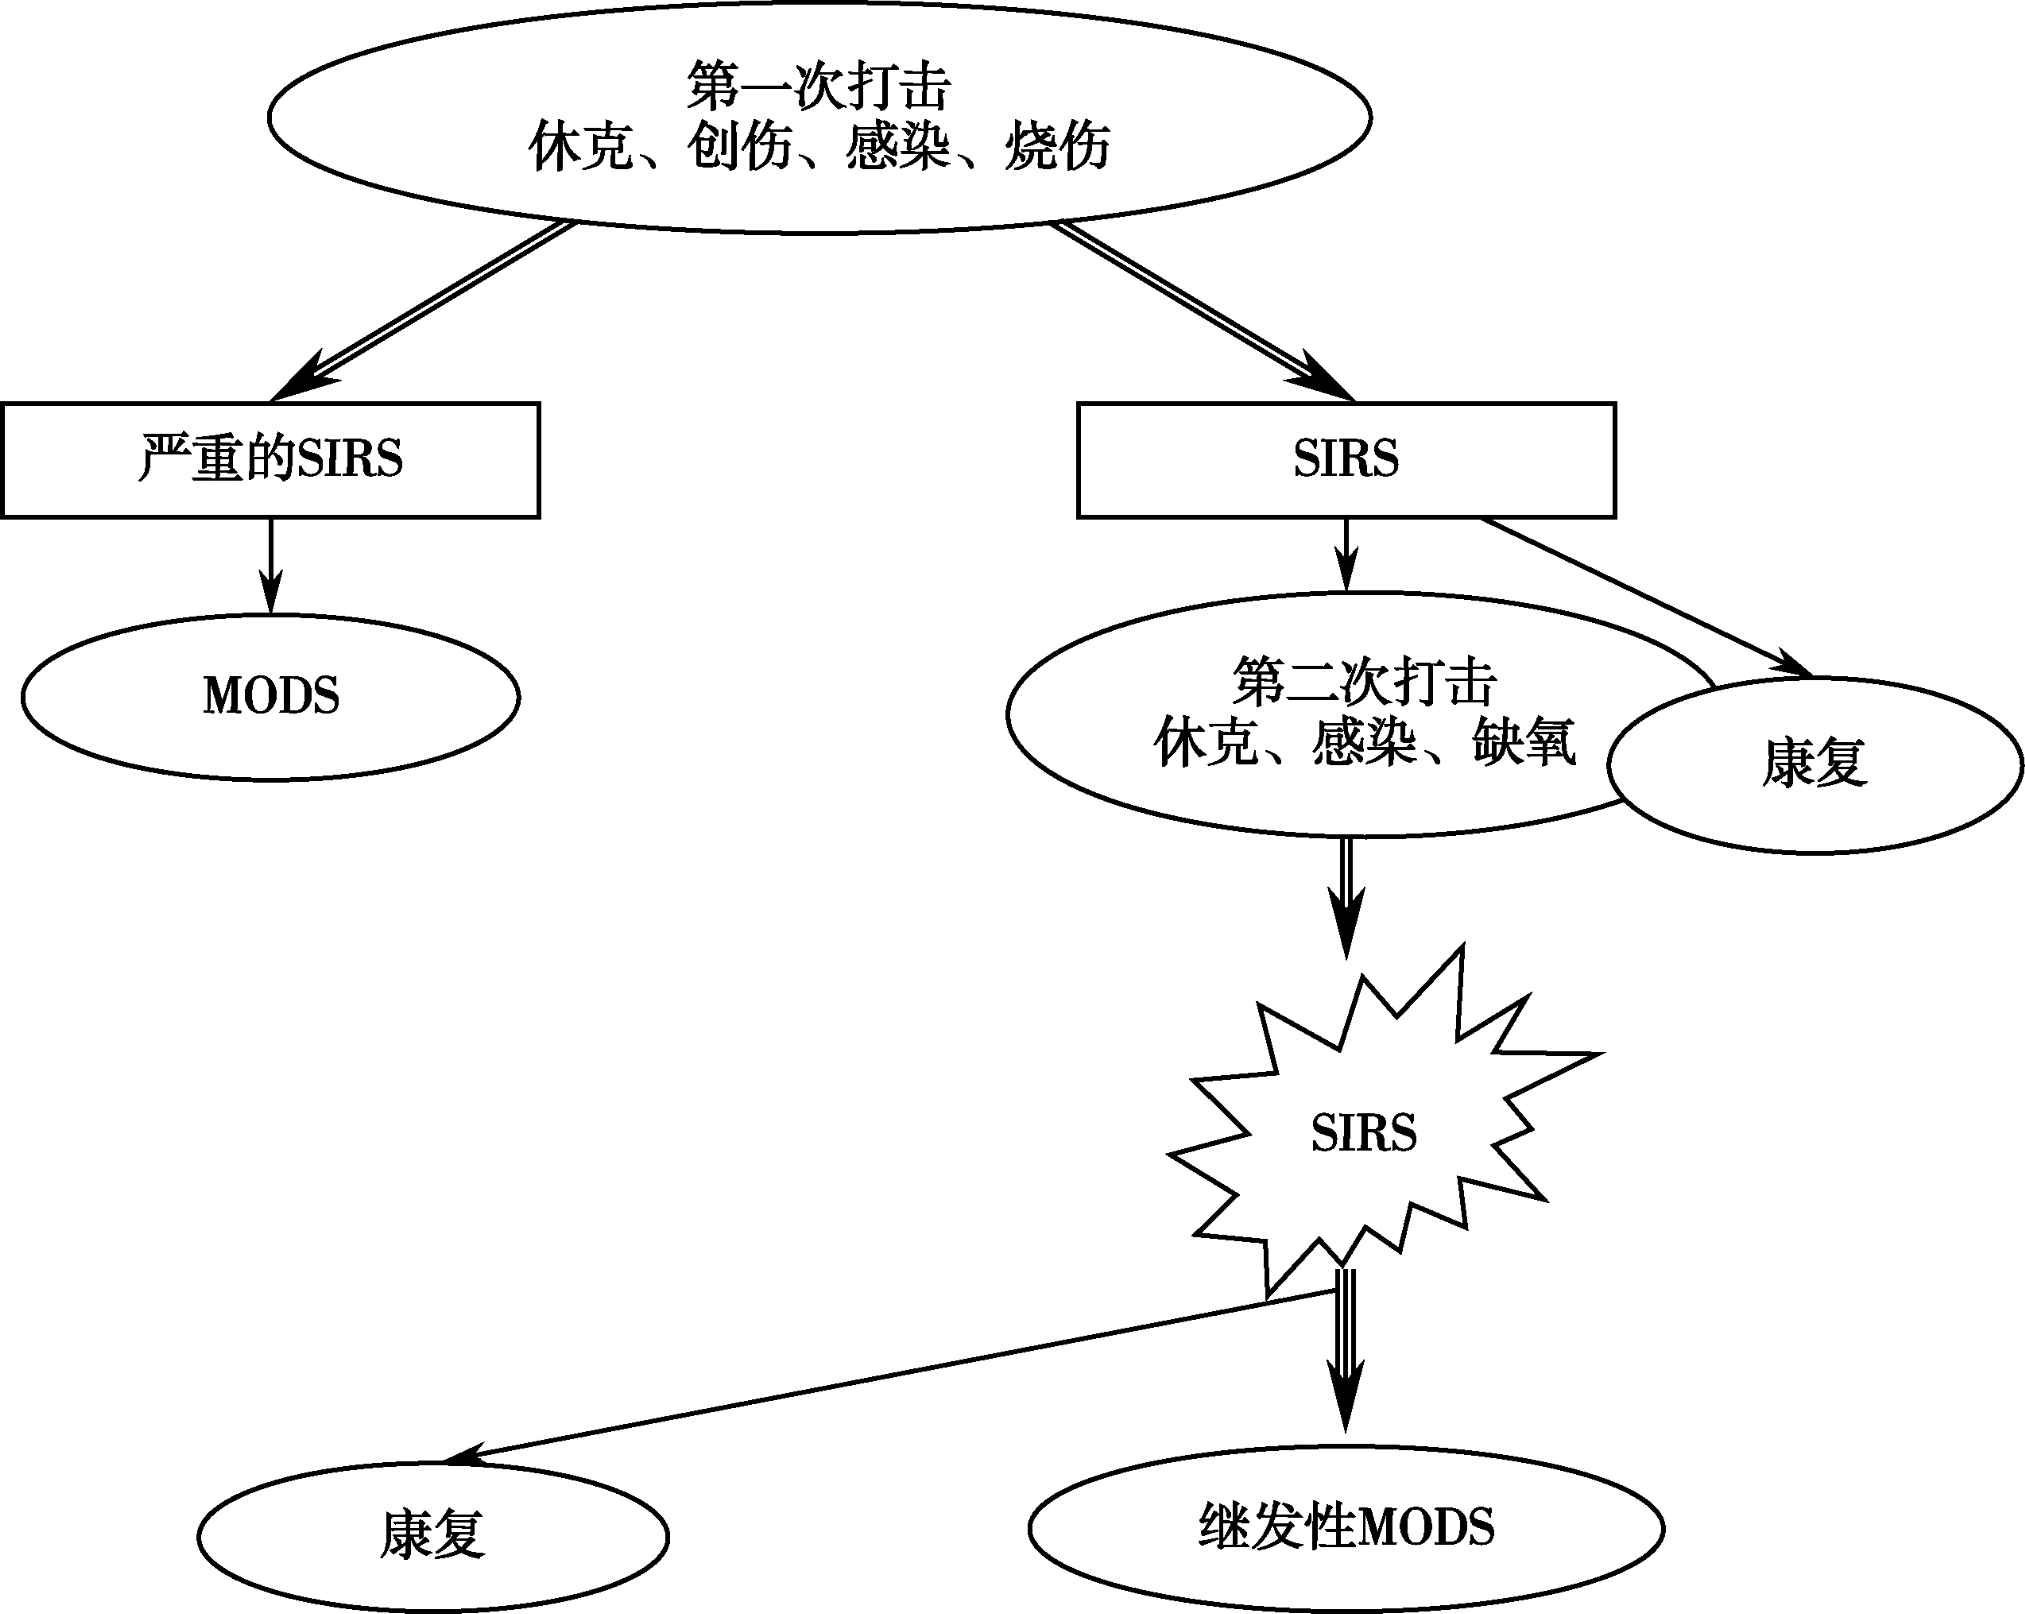
\includegraphics[width=4.23958in,height=3.38542in]{./images/Image00134.jpg}
 \captionsetup{justification=centering}
 \caption{多器官功能障碍综合征的二次打击学说}
 \label{fig35-3}
  \end{figure} 

危重患者的病情往往是复杂的,机体遭受打击次数可能是两次,也可能是多次。多次反复打击将使机体炎症反应放大和失控更易发生,使患者更易发生MODS。另外,不仅机体免疫系统参与多次打击导致MODS的病理生理过程,凝血、纤溶、补体、激肽等多个系统均参与或累及。

MODS二次打击学说的提出,进一步强调了感染、创伤的后期处理。后期处理不当,后果比早期损伤的结果更为严重,更具危害性。

\subsubsection{SIRS/CARS与MODS}

\hypertarget{text00093.htmlux5cux23CHP3-11-2-4-1}{}
(一) 炎症反应的意义

正常情况下
,炎症反应是防止组织损伤扩大,促进组织修复的以防御为主的局部组织反应,是机体修复和生存所必需的。感染和创伤触发机体炎症反应,如果炎症反应能够及时局限,清除细菌或异物,则对机体有益。如炎症反应不能局限,导致炎症反应失控,反而损伤自身组织,可能造成严重后果。

\hypertarget{text00093.htmlux5cux23CHP3-11-2-4-2}{}
(二) 全身性炎症反应综合征

1991年在芝加哥召开美国胸科医师学会和重症医学会(ACCP/SCCM)联席会议,将感染或创伤引起的持续全身炎症反应失控的临床表现命名为全身性炎症反应综合征(systemic
inflammatory response
syndrome,SIRS),并制定了相应的诊断标准(表\ref{tab35-3})。SIRS可由感染因素引起,若进行性加重可导致全身性感染(systemic
infection 或sepsis)、严重感染(severe
sepsis)、感染性休克、甚至MODS。SIRS也可由创伤、烧伤、急性重症胰腺炎等非感染因素引起,进行性加重亦可引起MODS。SIRS是感染或非感染因素导致机体过度炎症反应的共同特征,MODS是SIRS进行性加重的最终后果。因此,就本质而言,SIRS是导致MODS的共同途径。

\begin{table}[htbp]
\centering
\caption{全身性炎症反应综合征的诊断标准(符合下列两项或两项以上)}
\label{tab35-3}
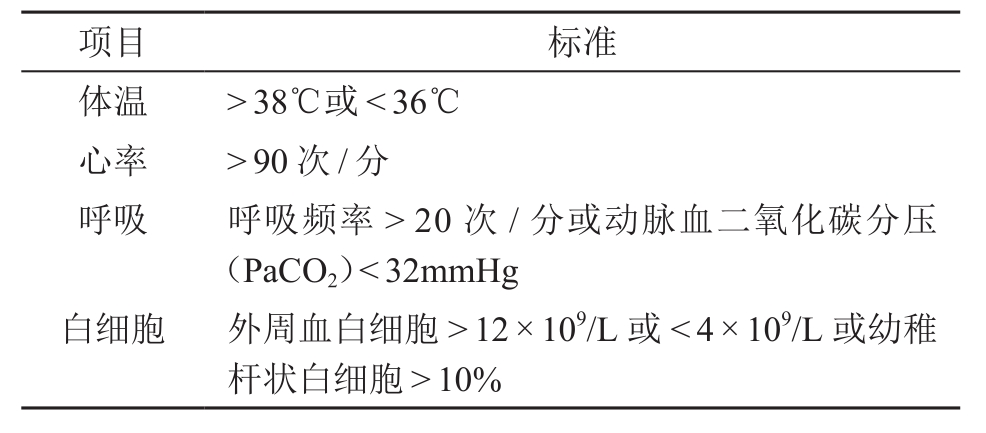
\includegraphics[width=3.28125in,height=1.4375in]{./images/Image00135.jpg}
\end{table}

SIRS的提出是对感染、创伤及MODS认识的重大突被和进展。导致MODS临床和基础研究的重点从感染、创伤本身转移到机体炎症反应这一本质上,同时也使MODS治疗手段从控制感染、创伤,延伸到调节机体炎症反应上。

对SIRS临床认识和理解的重要性远比SIRS的临床诊断重要。SIRS这一概念在临床应用中存在诸多问题:①诊断标准的敏感度过高:根据Rangel-Frausto的研究,3708例ICU及普通病房患者的SIRS发生率高达68\%。笔者的研究结果也显示ICU患者在转入时,有71.3\%符合SIRS诊断标准。这些研究提示SIRS发生率异常之高,使“SIRS”概念似乎与“危重病”的概念类似,即SIRS的诊断灵敏度高,而缺乏特异性。②难以反映疾病严重程度:临床研究中不能以SIRS判断疾病的严重程度,在1991年芝加哥会议上已认识到这一问题,因此,提出将SIRS与疾病严重程度评分相结合,对危重患者进行判断和治疗。当然,也有一些研究认为,SIRS符合四项指标的多少,与SIRS的严重程度及危重患者预后有关。③削弱或忽视寻找感染灶和控制感染:表现SIRS或“全身性感染”的患者,部分患者可能无感染灶,其“全身性感染”表现由创伤、急性重症胰腺炎或烧伤等非感染因素引起,但也有部分存在明确或可疑感染灶,例如,肺炎、腹腔感染等。因此,对于表现有SIRS的患者,不能仅仅满足于SIRS的诊断,要高度关注引起SIRS的原因,特别是是否有感染发生。

尽管SIRS概念的提出是MODS认识上的重大进步,但SIRS的诊断标准本身存在许多不足,特别是把它作为一个综合征或疾病时,不能停留在SIRS水平上,应积极寻找导致SIRS的致病因素。当然,我们并不能因为SIRS诊断标准存在问题而否认SIRS的重要意义。

\hypertarget{text00093.htmlux5cux23CHP3-11-2-4-3}{}
(三) 代偿性抗炎反应综合征

基于
SIRS是导致MODS的本质性原因这一认识,抑制SIRS有可能阻断炎症反应发展,最终可能降低MODS病死率。20世纪90年代初期,大量的动物实验研究显示,抑制炎症介质,明显降低感染或内毒素血症动物的病死率,为临床MODS的救治带来希望。令人失望的是,内毒素单抗、TNFα单抗等炎症介质拮抗剂在临床试验中相继失败,甚至个别研究报道增加病死率。由此迫使人们深入研究,并重新认识SIRS在MODS中的作用。首先引起注意的是机体受细菌毒素、损伤打击后,出现一过性细胞免疫功能降低,使机体对感染易感。其次,机体受细菌毒素、损伤刺激后,不仅释放炎症介质引起SIRS,同时大量释放内源性抗炎介质。后者可能是导致机体免疫功能损害的主要原因。第三,临床上盲目使用炎症介质拮抗剂,可能使免疫功能损伤加重,或许这就是炎症介质拮抗剂临床试验失败的主要原因。鉴于上述认识,1996年Bone针对感染或创伤时,导致机体免疫功能降低的内源性抗炎反应,提出了代偿性抗炎反应综合征(compensatory
antiinflammatory response
syndrome,CARS)的概念。CARS作为SIRS的对立面,两者常常是不平衡的。如保持平衡,则内环境稳定得以维持,不会引起器官功能损伤。一旦SIRS/CARS失衡,将引起内环境失去稳定性,导致组织器官损伤,发生MODS。

如果把SIRS和CARS看作机体炎症反应天平的两端,则CARS作为天平的另一端,对SIRS发生、发展所起的关键性作用是不言而喻的。CARS的发生主要与抗炎性介质合成、抗炎性内分泌激素及炎症细胞凋亡等因素有关。

\subparagraph{多种内源性抗炎介质参与 CARS}

单核巨噬细胞被过度激活后,不仅释放大量的促炎性介质,引起广泛的组织的自身性破坏,同时,也释放一种强烈的内源性免疫抑制剂------前列腺素(PG)E\textsubscript{2}
,引起细胞免疫功能瘫痪。临床研究证实,严重创伤或感染早期,单核细胞等可释放大量PGE\textsubscript{2}
,并持续升高长达21天。PGE\textsubscript{2}
通过抑制T辅助细胞(TH)向TH\textsubscript{1}
细胞分化,促使向TH\textsubscript{2}
细胞分化,从而抑制IL-2和IFNγ释放及IL-2受体表达,抑制细胞免疫功能;同时PGE\textsubscript{2}
诱导TH\textsubscript{2}
细胞及单核巨噬细胞释放IL-4、IL-10、IL-13等抗炎介质,强烈抑制TNFα、IL-1β等炎症介质释放。可见,PGE\textsubscript{2}
强烈抑制机体免疫功能,对抗SIRS。另外,IL-4和IL-10对炎症介质释放具有明显抑制作用,也是引起CARS的抗炎介质。临床研究发现IL-4和IL-10水平升高与创伤患者感染发生率呈正相关。另外,TNF可溶性受体、IL-1受体拮抗剂(IL-1ra)、超氧化物歧化酶、α1-抗胰蛋白酶等物质均属于内源性抗炎物质的范畴,参与CARS的发生。

\subparagraph{糖皮质激素和儿茶酚胺是参与 CARS的重要抗炎性内分泌激素}

糖皮质激素对免疫功能具有强烈非特异性抑制作用,明显抑制TNFα、IL-1β等炎症介质的释放,是导致CARS的重要原因。对于CARS占主导地位的MODS,糖皮质激素治疗不可能获得积极疗效。去甲肾上腺素和肾上腺素等内源性儿茶酚胺物质对内毒素诱导的炎症介质释放亦具有明显抑制作用。

\subparagraph{炎症细胞的凋亡是影响 CARS的重要因素}

粒细胞是重要的炎症细胞,其存活时间长短直接影响炎症反应的程度。正常情况下,粒细胞在循环中存活时间不超过24小时。内毒素及IL-1β、IL-8等与粒细胞结合,均使粒细胞凋亡延迟。当Fas和P55表达时,则粒细胞凋亡就会加速,使炎症趋于局限。可见,粒细胞凋亡加速也是CARS的重要机制,应引起重视。

CARS具有重要的临床意义。炎症无疑是消灭入侵病原体和异物的防御反应,但炎症反应过度又难免损害宿主自身。CARS的意义就在于限制炎症,保护宿主免受炎症的损害。机体受细菌/内毒素刺激后,引起炎症细胞活化和炎症介质的生成;与此同时,机体动员抗炎机制限制这种活化,这就是正常体内的炎症和抗炎症的平衡及其在机体自稳中的作用。当炎症刺激过强或持续刺激时,则导致炎症反应过度,超过CARS,SIRS/CARS平衡失调,则发生自身性破坏。反之,抗炎反应过强,又可导致CARS或免疫功能低下。

CARS以机体免疫功能低下为特征,但临床难以判断。为了使CARS应用于临床,1997年Bone提出CARS的诊断标准,即外周血单核细胞HLA-DR的表达量低于30\%,而且伴有炎症性细胞因子释放减少。同时,Bone指出,如果患者同时存在SIRS和CARS,则诊断为混合性炎症反应综合征(mixed
antagonistic response
syndrome,MARS)。CARS诊断标准有利于对炎症反应状态的判断,使SIRS/
CARS失衡理论应用于临床。

\hypertarget{text00093.htmlux5cux23CHP3-11-2-4-4}{}
(四) SIRS/CARS失衡与MODS

就其本质而言,MODS是SIRS/CARS免疫失衡的严重后果。SIRS/CARS失衡导致MODS的发展过程可分为3个阶段:①局限性炎症反应阶段:局部损伤或感染导致炎症介质在组织局部释放,诱导炎症细胞向局部聚集,促进病原微生物清除和组织修复,对机体发挥保护作用;②有限全身炎症反应阶段:少量炎症介质进入循环诱发SIRS,诱导巨噬细胞和血小板向局部聚集。同时,由于内源性抗炎介质释放增加导致CARS,使SIRS与CARS处于平衡状态,炎症反应仍属生理性,目的在于增强局部防御作用;③SIRS/CARS失衡阶段:表现为两个极端,一是大量炎症介质释放入循环,刺激炎症介质瀑布样释放,而内源性抗炎介质又不足以抵消其作用,导致SIRS。另一个极端是内源性抗炎介质释放过多而导致CARS。SIRS/CARS失衡的后果是炎症反应失控,使其由保护性作用转变为自身破坏性作用,不但损伤局部组织,同时打击远隔器官,导致MODS。

认识的进步,必然预示着在治疗上取得突破。恢复SIRS和CARS的动态平衡可能是MODS治疗的关键。

\protect\hypertarget{text00094.html}{}{}

\section{多器官功能障碍综合征的诊断与临床特征}

尽管多器官功能衰竭和多器官功能障碍综合征(MODS)已引起临床医师的广泛重视,但缺乏权威的定义和统一的诊断标准,使多器官功能衰竭和MODS临床研究结果差异很大,特别是患病率和病死率的结果差异巨大(表\ref{tab35-4})。参照国际公认标准,采用统一的定义和诊断标准,显然是很有必要的。

\begin{table}[htbp]
\centering
\caption{多器官功能障碍综合征患者的病死率}
\label{tab35-4}
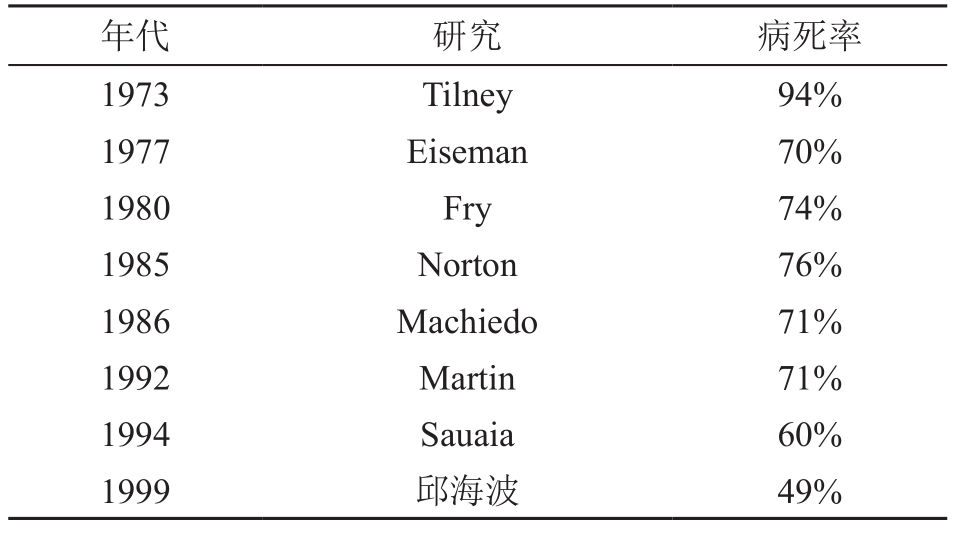
\includegraphics[width=3.20833in,height=1.78125in]{./images/Image00136.jpg}
\end{table}

\subsubsection{MODS的定义}

MODS是由严重感染、严重免疫炎症紊乱(如重症胰腺炎)、创伤、烧伤以及各种休克引起的,以严重生理紊乱为特征的临床综合征,其临床特征是多个器官序贯或同时发生功能障碍或功能衰竭。确切地说,MODS是在严重感染、创伤、烧伤、休克及重症胰腺炎等疾病过程中,发病24小时以上,出现2个或2个以上的器官或系统序贯性的功能障碍或功能衰竭。若在发病24小时内死亡者,则属于复苏失败,需排除。

在MODS的概念中,器官衰竭的类型、严重程度、累及范围及持续时间是特别需要关注的问题,这些问题也随着临床认识的深入而有所改变。早期的多器官功能衰竭定义,无论是Tilney提出的序贯性器官功能衰竭、Polk提出的远隔器官功能衰竭,还是Eiseman提出的多器官功能衰竭,集中体现多个特定器官的功能障碍,特别强调器官功能障碍的程度已达到衰竭。它们所反映的相同问题是将多器官功能衰竭看作是器官功能处于终末期的一个静态概念。与之相对应的多器官功能衰竭诊断标准,实际上也就成为筛选器官衰竭的标准。

任何疾病过程都是进行性的、渐进的病理生理过程,多器官功能衰竭也具有类似的特点。早期感染、创伤引起轻度的内环境紊乱,进行性发展出现器官功能的损害,当器官功能损害达到一定的严重程度时,则发生器官功能衰竭。对多器官功能衰竭的认识至少有两点值得反思:①多器官功能衰竭不是一个孤立的事件,具有较宽的内涵,实际上多器官功能衰竭也应当包括从早期内环境紊乱发生到多器官衰竭的连续的整个病理生理过程,但传统的多器官功能衰竭概念难以体现这一含义;②当患者诊断多器官功能衰竭时,器官功能衰竭已到晚期,常常痛失治疗时机,对多器官功能衰竭的早期干预,前提是对多器官功能衰竭的早期认识。对多器官功能衰竭的反思导致1991年美国胸科医师学会/重症医学会(ACCP/SCCM)提出MODS的概念,以代替多器官功能衰竭。这反映了人们对多器官功能衰竭更为深入的认识和了解,将MODS定义为一个包括早期病理生理改变到终末期器官功能衰竭的连续的完整的病理生理过程,确立了动态和开放的MODS概念,为MODS的早期认识、早期诊断以及早期干预奠定了基础,具有重要的临床意义。

MODS概念的提出是认识进步的结果,但确定较为合理的MODS定义仍然困难。为了避免割裂MODS整个病理生理过程,ACCP/SCCM提出了一个较为模糊的MODS定义,即各种疾病导致多个器官不能维持自身功能,从而影响全身内环境稳定性的状态。MODS表述的器官功能障碍可以是相对的,也可以是绝对的,而且器官功能障碍是动态的、连续的变化过程,对器官功能的动态观察必将有助于MODS的早期诊断和治疗。

针对机体炎症反应失控在MODS发病、发展中的根本性作用,MODS进一步被认为是炎症反应失控的表现和结果。1991年ACCP/SCCM联席会议同时提出了全身性炎症反应综合征(SIRS)的概念的诊断标准(参见表\ref{tab35-3}),MODS实际上就是全身性炎症反应引起的器官功能障碍。因此,MODS也可理解为SIRS
+器官功能障碍,而传统的多器官功能衰竭就是MODS继续发展的最严重的终末期结果。

尽管MODS的定义和诊断仍有许多模糊之处,但正是这种模糊的概念才能够较为全面地涵盖MODS的整个从轻到重的、进行性的、连续的、完整的病理生理过程。

\subsubsection{MODS的分类}

根据MODS器官功能障碍发生的主要原因以及SIRS在器官功能损伤中的地位,可将MODS分为原发性MODS和继发性MODS。

原发性MODS是指某种明确的损伤直接引起器官功能障碍,即器官功能障碍由损伤本身引起,在损伤早期出现。如严重创伤后,直接肺挫伤导致急性呼吸衰竭,横纹肌溶解导致肾脏功能衰竭,大量出血补液导致凝血功能异常。在原发性MODS的发病和演进过程中,SIRS在器官功能障碍发生中所占比重较低。

继发性MODS并非是损伤的直接后果,而与SIRS引起的自身性破坏关系密切。损伤引起SIRS,而异常的炎症反应继发性造成远距离器官发生功能障碍。所以,继发性MODS与原发损伤之间存在一定的间歇期,易合并感染。在继发性MODS中,SIRS是器官功能损害的基础,全身性感染和器官功能损害是SIRS的后继过程。SIRS-全身性感染-MODS就构成一个连续体,继发性MODS是该连续体造成的严重后果。

对于原发性MODS患者,当机体发生原发性器官功能损害后,如能够存活,则原发性损伤与原发性器官功能损害将刺激机体免疫炎症反应,导致全身性炎症反应,又可进一步加重器官功能障碍或引起新的严重器官功能损伤,实际上,MODS就从原发性转变为继发性。

\subsubsection{诊断标准}

\hypertarget{text00094.htmlux5cux23CHP3-11-3-3-1}{}
(一) 多器官功能衰竭和多器官功能障碍综合征的诊断标准

1980年Fry提出第一个多器官功能衰竭诊断标准。在此之前,循环、呼吸、肾脏和肝脏等器官已经具有单一器官衰竭的判断或诊断标准。应激性上消化道出血被认为是胃肠道功能衰竭。然而,血液、代谢和神经系统的衰竭或功能紊乱就缺乏明确的诊断方法。弥散性血管内凝血(DIC)显然是血液系统的功能紊乱,DIC诊断中除了出血等临床表现外,还需有血浆纤维蛋白降解产物水平升高。但血浆纤维蛋白降解产物浓度升高缺乏特异性,严重创伤或手术患者也可升高,使血液系统功能衰竭的诊断缺乏客观性。代谢紊乱是重症患者应激打击的结果,如果能够对代谢过程进行复杂的监测,则所有重症患者可能都存在所谓的“代谢障碍”,对代谢障碍的诊断缺乏可行性。神经系统功能障碍在重症患者中也很常见,但准确定量评价非常困难。另外,严重感染导致内脏器官严重损害时,往往血压和心输出量是正常或偏高的,直到出现休克或临终期,心血管系统才表现出功能衰竭。因此,Fry在提出多器官功能衰竭诊断标准时,仅包含了呼吸、肝脏、肾脏和胃肠道系统(表\ref{tab35-5})。

\begin{table}[htbp]
\centering
\caption{多器官功能衰竭诊断标准(Fry,1980年)}
\label{tab35-5}
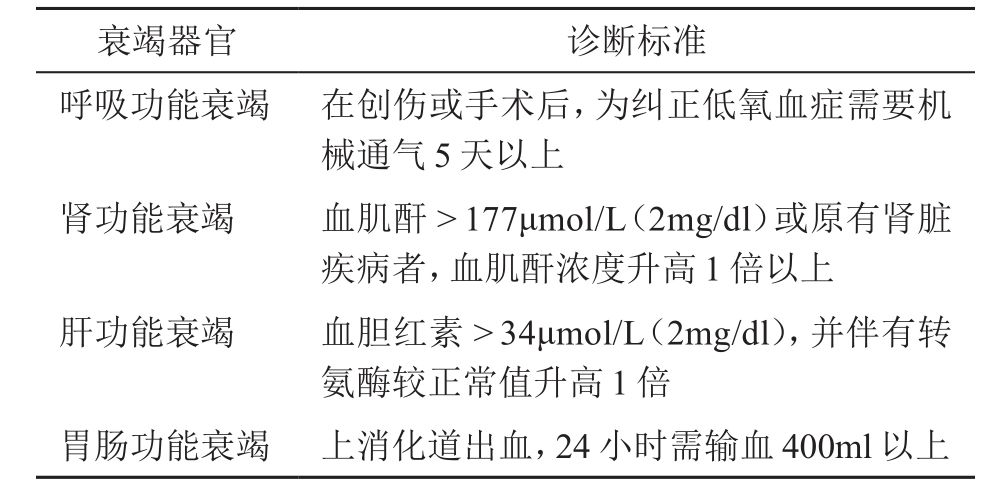
\includegraphics[width=3.3125in,height=1.625in]{./images/Image00137.jpg}
\end{table}

该诊断标准中,呼吸衰竭采用了Fulton的提法。即在创伤或手术后,为纠正低氧血症需要机械通气5天以上。许多患者在创伤、手术或复苏后,往往会出现低氧血症,需要机械通气给予支持。尽管第一天低氧血症最严重,但第二到第三天逐步进入恢复期,短期机械通气后即可脱机。因此,选择机械通气不短于5天作为呼吸衰竭的诊断标准,以排除早期的一过性低氧血症。

同时符合血胆红素>
34μmol/L(2mg/dl)和转氨酶较正常值升高1倍,作为肝脏功能衰竭的诊断标准,可排除假性的肝脏功能衰竭。即使肝脏未受损害,严重创伤患者非肝脏源性的转氨酶释放,也可导致转氨酶升高,而胆红素多不升高。同样,大量输血、腹膜后或盆腔血肿及胆道结石梗阻等常常引起单纯胆红素升高。胆红素和转氨酶同时升高诊断肝脏功能衰竭,可避免误诊。

尽管少尿或无尿是急性肾衰竭最突出表现,肾脏功能衰竭采用了血肌酐>
177μmol/L(2mg/dl)或原有肾脏疾病者,血肌酐浓度升高1倍以上为诊断标准,而未包含尿量的指标。一方面,部分急性肾衰竭患者为非少尿型,以少尿来诊断急性肾衰竭显然会漏诊;另一方面,当急性肾衰竭患者发生少尿时,血肌酐可能高达442~707μmol/L(5~8mg/dl),如以少尿为诊断标准,则会延误诊断,不利于急性肾衰竭早期治疗。

以上消化道出血为特征的胃肠道功能衰竭是重症患者的常见并发症。由于急诊床边消化内镜在ICU未普遍开展,只能以24小时需输血400ml以上作为上消化道出血的间接诊断。如能够实施床边紧急消化内镜检查,则有助于明确诊断。

尽管Fry的多器官功能衰竭诊断标准是目前被公认的、应用最普遍的诊断标准,仍然存在很多问题。①该标准未包括神经系统、循环系统、血液系统等常见的器官功能衰竭;②以终末期的功能衰竭为诊断标准,不利于早期诊断和治疗;③难以反映多器官功能衰竭动态连续变化的病理生理过程;④呼吸功能衰竭的诊断过于严格,容易漏诊。

针对Fry诊断标准存在的问题,邱海波等于1997年提出了修正的Fry-MODS诊断标准(表\ref{tab35-6})。该标准结合国际常用的诊断标准,几乎包括了所有可能累及的器官或系统。当然,该标准未能包括MODS的整个病理生理过程,但避免烦琐的程度评分,较为简捷,增加了临床实用性。

\begin{table}[htbp]
\centering
\caption{多器官功能障碍综合征诊断标准}
\label{tab35-6}
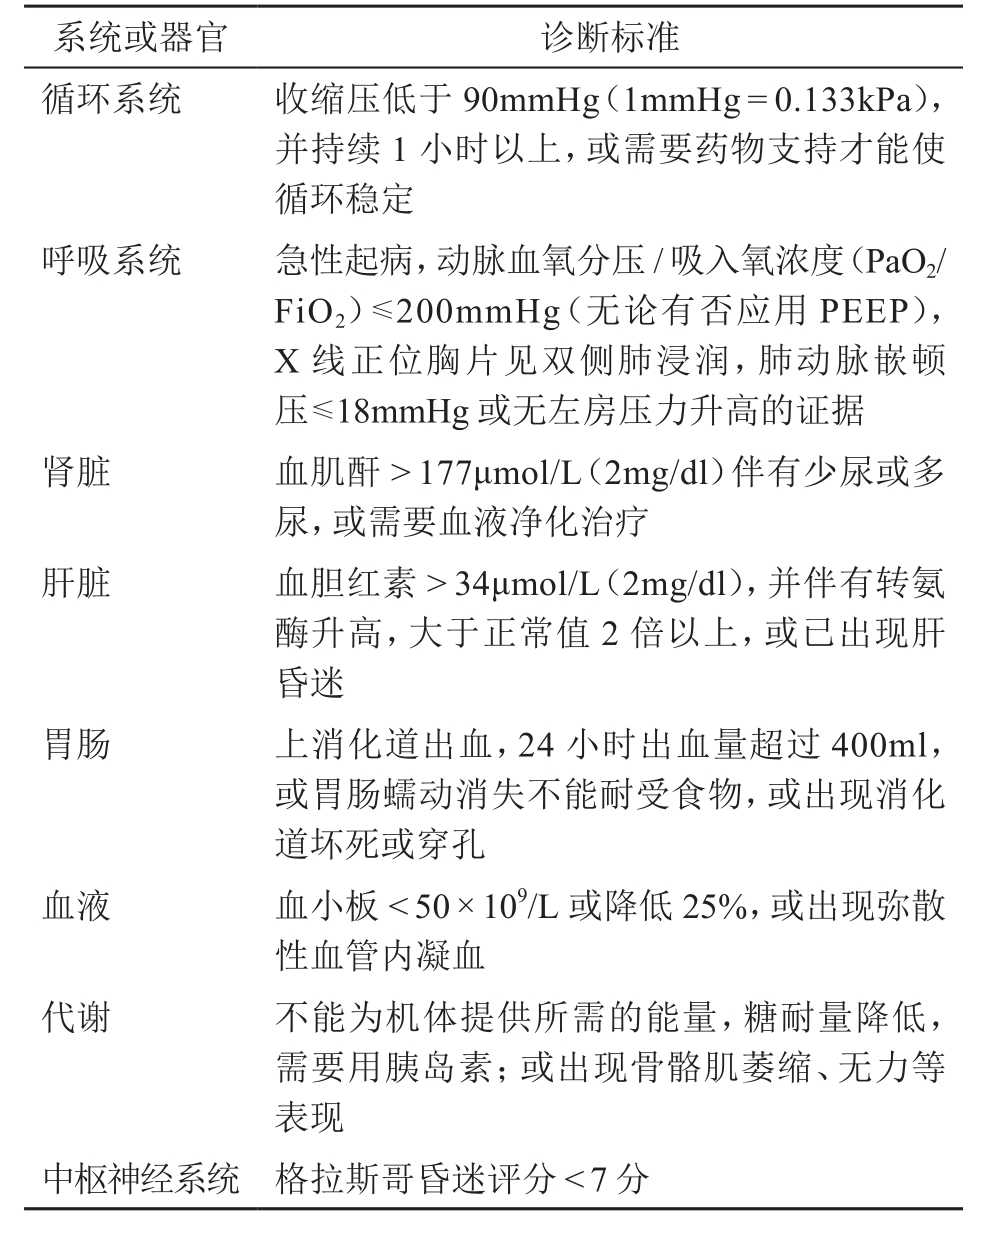
\includegraphics[width=3.3125in,height=4.10417in]{./images/Image00138.jpg}
\end{table}

\hypertarget{text00094.htmlux5cux23CHP3-11-3-3-2}{}
(二) 反映 MODS病理生理过程的疾病特异性诊断标准

对MODS病理生理过程认识的进步,也体现在MODS的诊断标准方面。计分法诊断标准是定量、动态评价MODS病理生理过程的较理想手段。但简捷准确是计分法标准是否实用的关键。1995年Marshall和Sibbald提出的计分法MODS诊断评估系统值得推广(表\ref{tab35-7})。通过每天作MODS评分,可对MODS的严重程度及动态变化进行客观的评估。

\begin{table}[htbp]
\centering
\caption{多器官功能障碍综合征计分法评估系统}
\label{tab35-7}
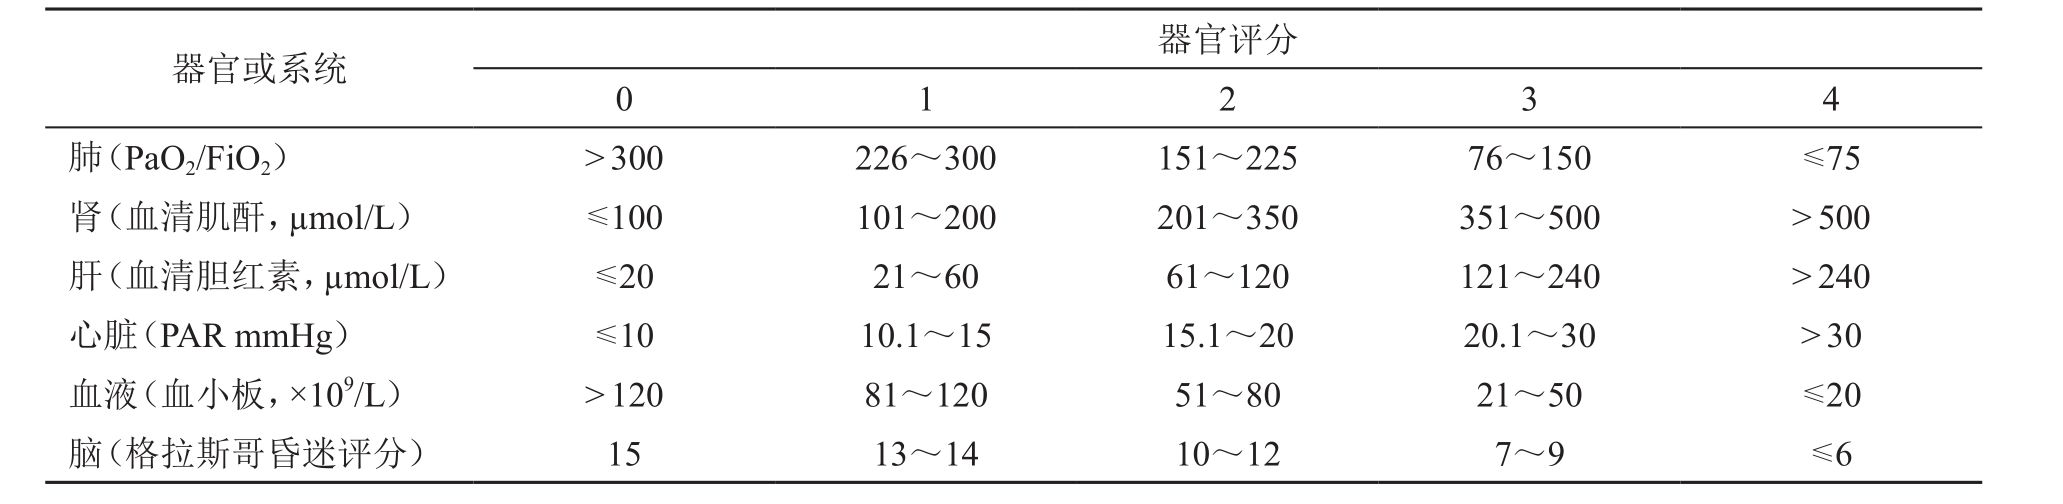
\includegraphics[width=6.86458in,height=1.66667in]{./images/Image00139.jpg}
\end{table}

PAR(pressure-adjusted heart
rate):压力校正心率=心率×右房压(或中心静脉压)/平均动脉压;如应用镇静剂或肌松剂,除非存在神经功能障碍的证据,否则应视作正常计分

Marshall提出的MODS计分法评估系统中,MODS分数与病死率呈显著正相关(表\ref{tab35-8}),对临床MODS的预后判断具有指导作用。

\begin{table}[htbp]
\centering
\caption{MODS评分与预计病死率}
\label{tab35-8}
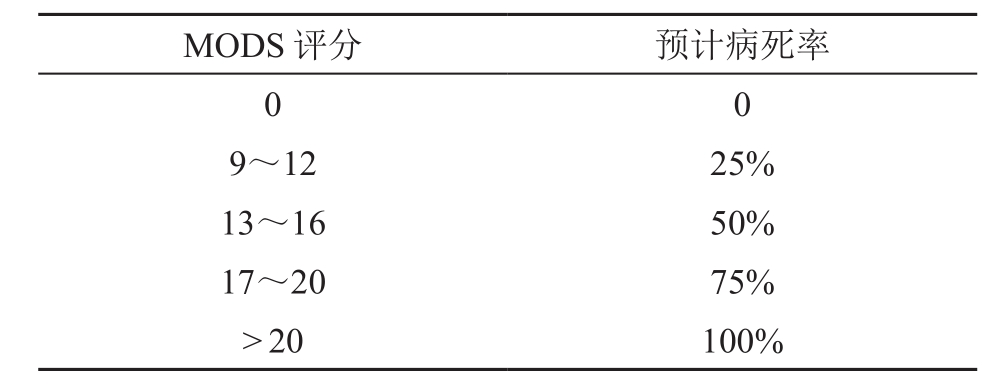
\includegraphics[width=3.29167in,height=1.29167in]{./images/Image00140.jpg}
\end{table}

不同疾病导致的MODS具有不同特点,建立疾病特异性的MODS评分和诊断系统,是MODS深入研究的结果。1996年Vincent等提出了全身性感染相关性器官功能衰竭评分(SOFA),它不但体现器官和系统功能衰竭的病理生理过程和程度评价,而且也是对疾病(感染)特异性的MODS进行评估(表\ref{tab35-9})。

\hypertarget{text00094.htmlux5cux23CHP3-11-3-3-3}{}
(三) MODS诊断标准的片面性

尽管MODS的诊断标准已经能够初步的反映器官功能障碍的病理生理过程,但仍然存在片面性。

1.任何一个
MODS诊断标准,均难以反映器官功能衰竭的病理生理内涵。机体免疫炎症反应紊乱在MODS发生发展中具有关键性作用,但必须通过实验室检查才能够了解免疫功能紊乱的程度,目前还缺乏临床判断指标。对于神经系统功能评估,即使患者格拉斯哥昏迷评分低于6分,我们也很难肯定患者存在严重的神经系统功能障碍。对胃肠道功能衰竭的诊断就更显得复杂和难以确定,当肠系膜动脉灌注明显减少导致肠道缺血时,肠黏膜屏障功能受损,肠道细菌和毒素就能够发生移位,可能引起休克和呼吸衰竭。此时,我们仅仅关注患者发生呼吸循环衰竭,而关键性的胃肠道功能衰竭却被忽视。看来,很难给胃肠道功能衰竭确定一个准确的诊断标准。肝脏功能障碍也面临类似的问题,无论是伴黄疸的肝胆功能障碍,还是全身性的内毒素血症,均可导致肝脏库普弗细胞激活,炎症反应的暴发,临床上可能首先出现循环衰竭,肝脏功能及肝脏免疫功能的改变因缺乏临床表现而被遗漏。

\begin{table}[htbp]
\centering
\caption{全身性感染相关性器官功能衰竭评分标准(SOFA)}
\label{tab35-9}
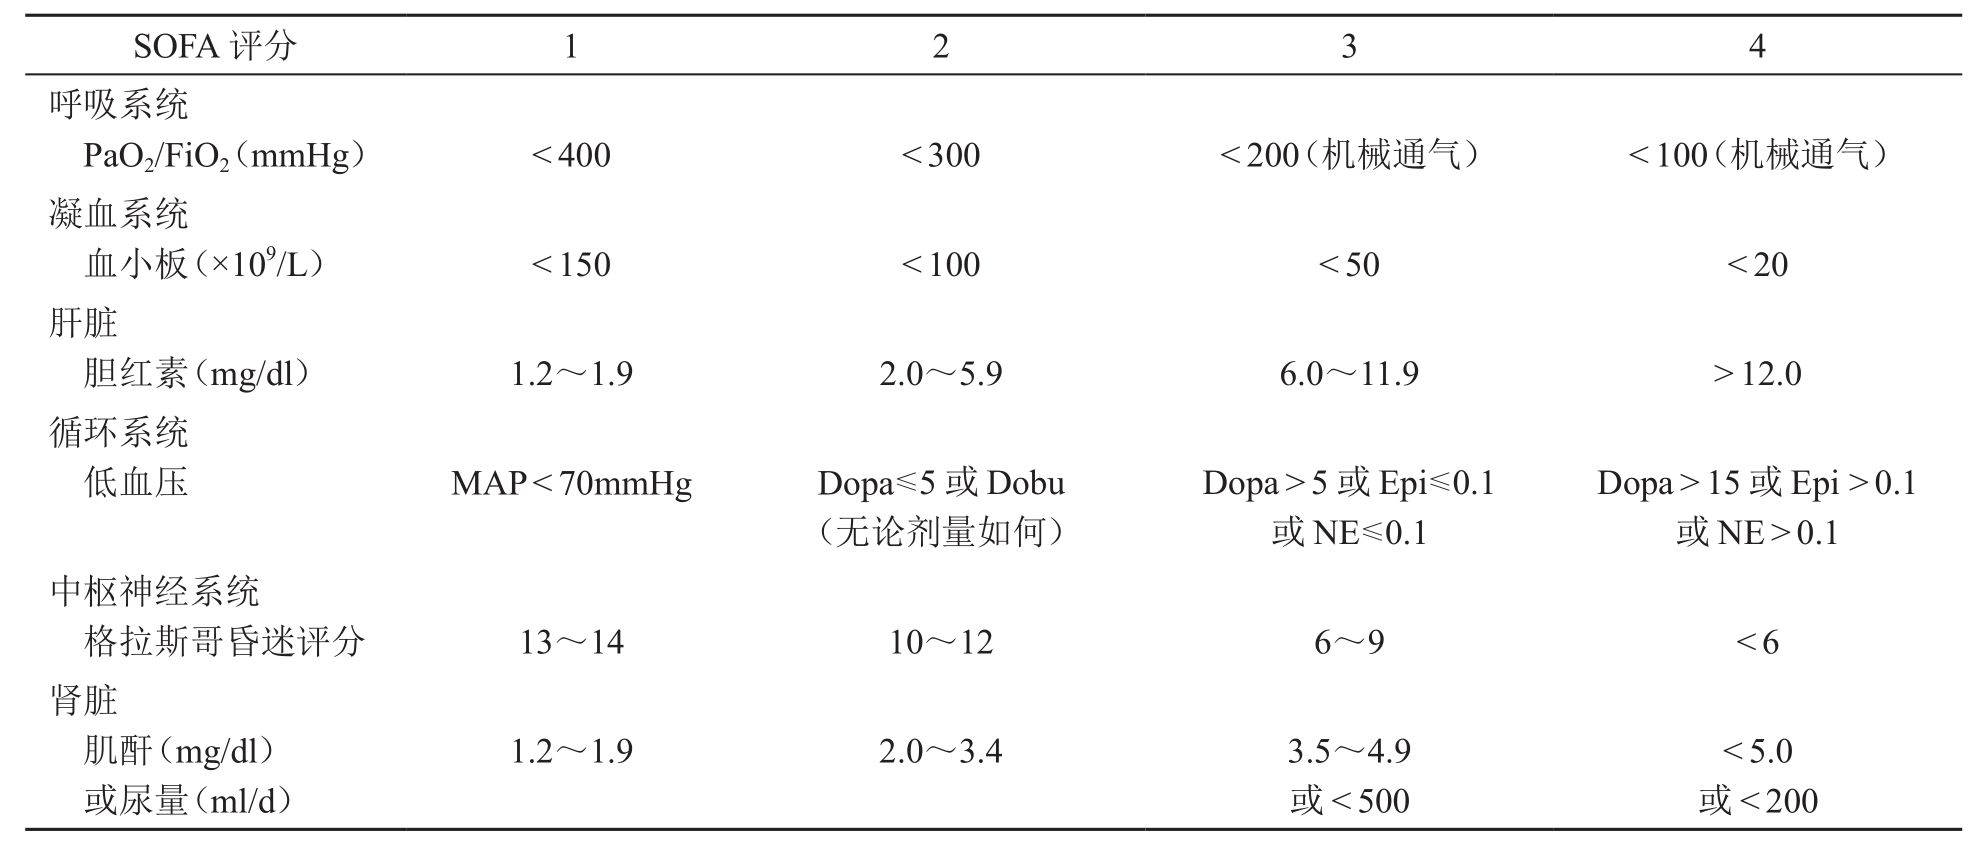
\includegraphics[width=6.60417in,height=2.80208in]{./images/Image00141.jpg}
\end{table}

MAP为平均动脉压,Dopa为多巴胺,Dobu为多巴酚丁胺,Epi为肾上腺素,NE为去甲肾上腺素

2.目前的
MODS诊断标准容易使临床医师产生误解,将MODS看作是功能障碍或功能衰竭器官的简单叠加,而忽视了MODS的病理机制以及器官之间互相作用的重要性。强调各个单一器官功能衰竭对重症患者的病情判断和治疗无疑是很重要的,但MODS并不是各个单一器官功能障碍的简单叠加,同样是两个器官衰竭,但器官不同,对MODS患者的影响也不同。Knaus的大规模调查显示循环衰竭合并血液系统衰竭时,MODS患者的病死率为20\%,而循环衰竭合并神经系统功能衰竭时,病死率可高达76\%。另外,器官简单叠加的MODS诊断标准也难以反映某一器官衰竭或损伤后,对机体炎症反应的刺激和放大效应,而正是放大失控的炎症反应导致器官功能损害的恶化或导致MODS。还需注意的是MODS的临床表现和实验室检查结果(如血清胆红素或血肌酐),尽管在一定程度上反映了相关器官和组织功能受损的程度,但这仅仅是MODS机体自身性破坏的部分表象而已,难以说明器官功能损害的本质性原因。因此,有必要强调MODS各器官之间的相互作用,从病理生理机制的角度制定合理的MODS诊断标准,将有助于深刻了解MODS病理生理学变化,更全面、更深入的认识MODS。

\subsubsection{MODS的临床特征}

尽管MODS的临床表现很复杂,但在很大程度上取决于器官受累的范围及损伤是由一次打击还是由多次打击所致。MODS临床表现的个体差异很大,一般情况下,MODS病程大约14~21天,并经历4个阶段,包括休克、复苏、高分解代谢状态和器官衰竭阶段。每个阶段都有其典型的临床特征(表\ref{tab35-10}),且发展速度极快,患者可能死于MODS的任一阶段。

尽管MODS涉及面广,临床表现复杂,但MODS具有以下显著特征:①发生功能障碍的器官往往是直接损伤器官的远隔器官。②从原发损伤到发生器官功能障碍在时间上有一定的间隔。③高排低阻的高动力状态是循环系统的特征。④高氧输送和氧利用障碍及内脏器官缺血缺氧,使氧供需矛盾尖锐。⑤持续高代谢状态和能源利用障碍。

\subsubsection{MODS的流行病学}

\hypertarget{text00094.htmlux5cux23CHP3-11-3-5-1}{}
(一) MODS的患病情况

\subparagraph{MODS患病率}

MODS是导致ICU重症患者死亡的首要原因。根据1988~1990年美国40家医院17
449例ICU患者的统计调查结果,MODS患病率为14\%。早期认识MODS患病危险因素,早期干预,仍然是重症医学的重要研究方向。

\begin{table}[htbp]
\centering
\caption{多器官功能障碍综合征的临床分期和特征}
\label{tab35-10}
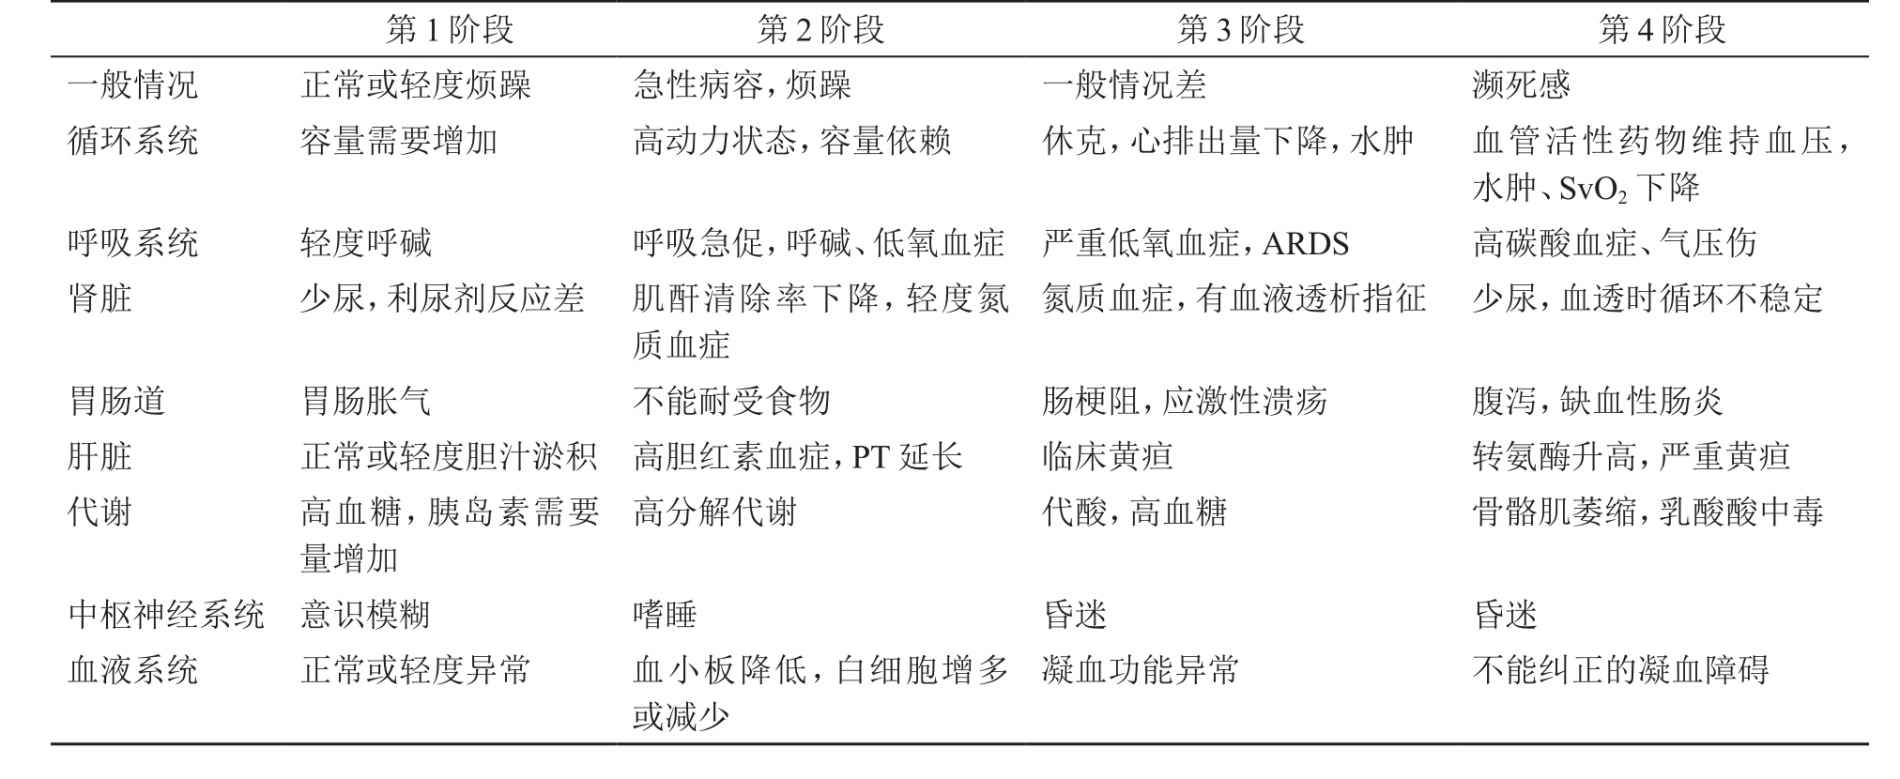
\includegraphics[width=6.73958in,height=2.76042in]{./images/Image00142.jpg}
\end{table}

\subparagraph{MODS衰竭器官及衰竭顺序}

MODS患者不同器官发生功能障碍的频率是不同的。北京协和医院的调查显示以呼吸和循环衰竭发生频率最高,分别为81.7\%和81.42\%,其次依次为中枢神经系统功能衰竭55.5\%、胃肠功能衰竭39.8\%、肾功能衰竭38.4\%、肝功能衰竭17.9\%和血液系统功能衰竭11.2\%。

MODS的各器官功能障碍的始发时间不同,一般无特定发病顺序。但在同类疾病引起的MODS中,器官功能障碍的顺序似乎有规律可循。有研究表明外科急诊手术后合并感染的患者,一旦发生MODS,器官功能障碍的顺序有一定的规律。以急诊手术当天为起点,术后2.6天发生全身性感染,呼吸功能衰竭是第一个发生功能障碍的器官,几乎与全身性感染的时间一致。之后,依次发生肝脏、胃肠道和肾脏功能衰竭(表\ref{tab35-11})。MODS器官发生功能障碍顺序有助于临床医师早期认识和预防可能发生的器官功能障碍。当然,由于患者个体差异很大,即使原发疾病相同,MODS发生功能障碍的器官顺序也可能有较大差异。

\begin{table}[htbp]
\centering
\caption{多器官功能障碍综合征患者器官功能衰竭的发生顺序}
\label{tab35-11}
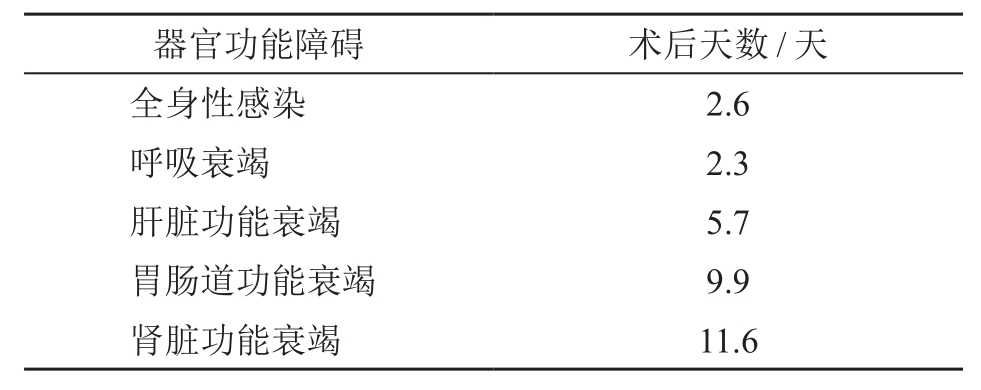
\includegraphics[width=3.26042in,height=1.29167in]{./images/Image00143.jpg}
\end{table}

\hypertarget{text00094.htmlux5cux23CHP3-11-3-5-2}{}
(二) 预后及病死率

MODS是住院患者首要死亡原因,而且MODS的病死率与器官衰竭数目具有明显的相关性(表\ref{tab35-12})。根据美国1988~1990年42家医院17
440例ICU患者的统计,2个器官衰竭者病死率52\%~65\%,而3个或3个以上者病死率达84\%。北京协和医院对1991~1996年1056例ICU患者的调查显示,MODS病死率49.3\%,其中2个器官衰竭者病死率17.8\%,3个器官衰竭者病死率47.1\%,而4个器官衰竭者病死率达77\%。可见,患者一旦发生MODS,病死率很高,严重影响其预后。

\begin{table}[htbp]
\centering
\caption{多器官功能障碍综合征患者的患病率及病死率}
\label{tab35-12}
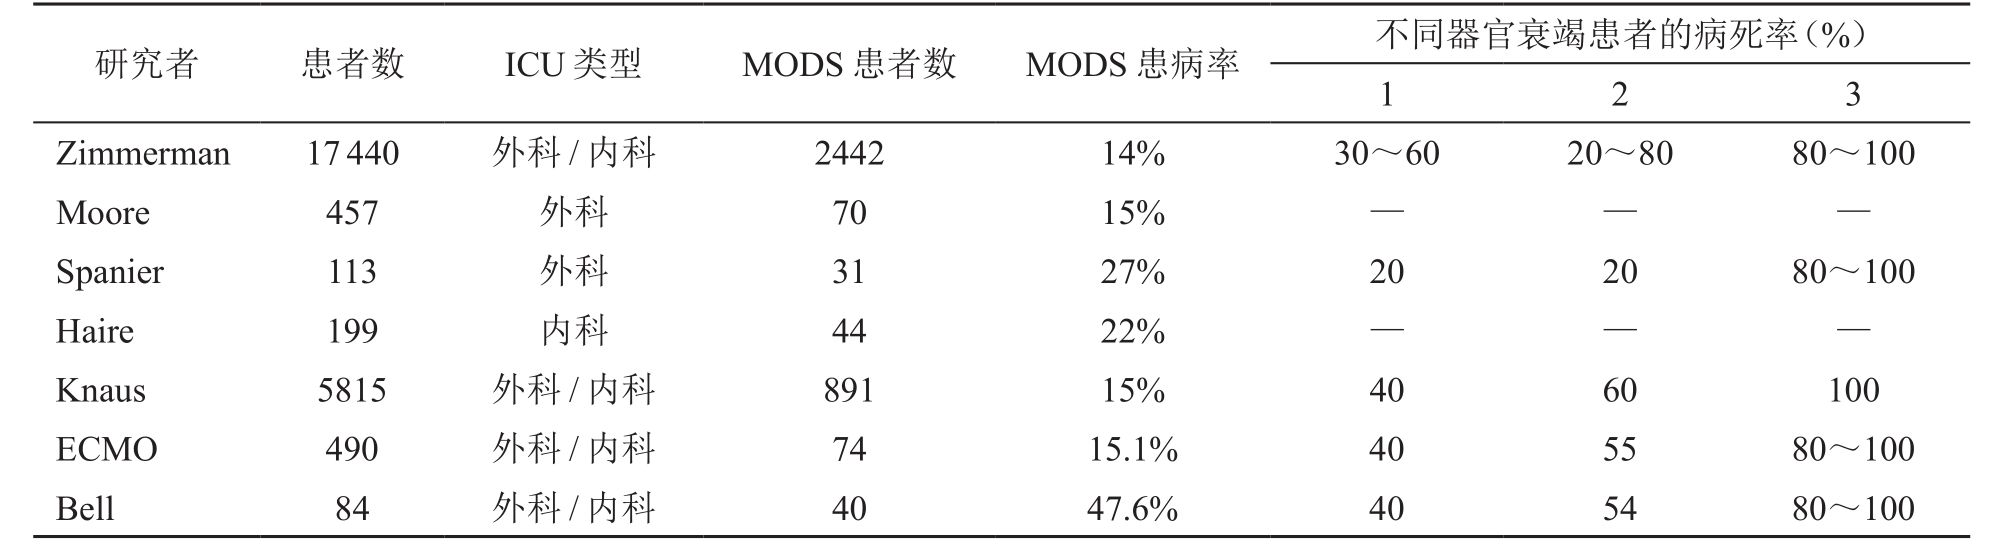
\includegraphics[width=6.64583in,height=1.84375in]{./images/Image00144.jpg}
\end{table}

尽管衰竭器官数量相同,但衰竭器官不同,MODS病死率也可能不同。北京协和医院ICU的调查显示118例患者发生2个器官功能衰竭,病死率为17.8\%,但衰竭器官不同,病死率差异很大。呼吸和循环衰竭者病死率19.5\%,而肝肾功能衰竭者病死率高达33.3\%(P
< 0.05)。

Zimmerman等报道3个或3个以上器官衰竭者的病死率,1979~1982年为98\%,1988~1990年降低至84\%。1990年以来,MODS病死率是否进一步降低呢?北京协和医院ICU观察了1991~1996年MODS病死率变化,结果显示6年来MODS病死率无明显改变。为排除人群构成和基本疾病差异性的影响,分别以年龄和APACHE
Ⅱ评分对逐年的病死率作调整,结果6年期间的调整率亦无显著差异。说明1990年以来,MODS病死率依然居高不下,也从一个侧面反映了当前器官功能支持治疗手段并不能进一步降低MODS的病死率,必须寻求新的治疗途径。

\hypertarget{text00094.htmlux5cux23CHP3-11-3-5-3}{}
(三) 病死危险因素

MODS患者病死率高,认识病死危险因素,有助于早期确立MODS治疗对策。Knaus等学者对MODS的病死危险因素作了大规模的临床调查,概括了MODS病死的相关危险因素(表\ref{tab35-13})。针对MODS病死危险因素进行积极处理和干预,可能是降低MODS病死率的关键。

\begin{table}[htbp]
\centering
\caption{多器官功能障碍综合征的病死危险因素}
\label{tab35-13}
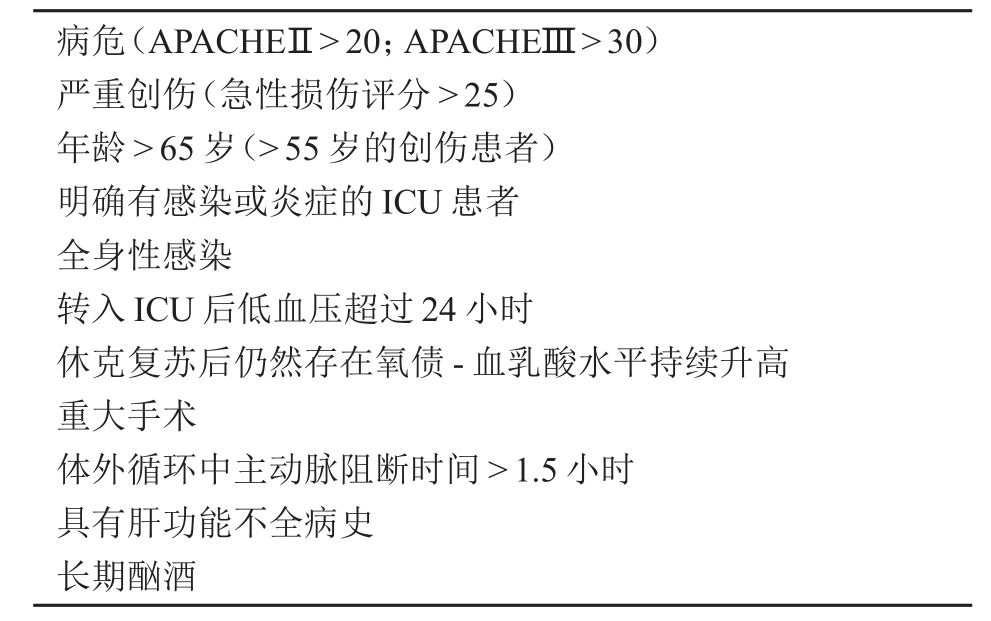
\includegraphics[width=3.29167in,height=2.0625in]{./images/Image00145.jpg}
\end{table}

\hypertarget{text00094.htmlux5cux23CHP3-11-3-5-4}{}
(四) MODS患者的直接病死原因

循环功能衰竭(以感染性休克为主)为MODS最常见的直接病死原因,其次为中枢神经系统功能衰竭和心功能衰竭等(表\ref{tab35-14})。进一步提示在MODS治疗中,应特别注意纠正循环衰竭,并针对病因采取有效治疗措施,不应掉以轻心。

\begin{table}[htbp]
\centering
\caption{多器官功能障碍综合征患者的直接病死原因}
\label{tab35-14}
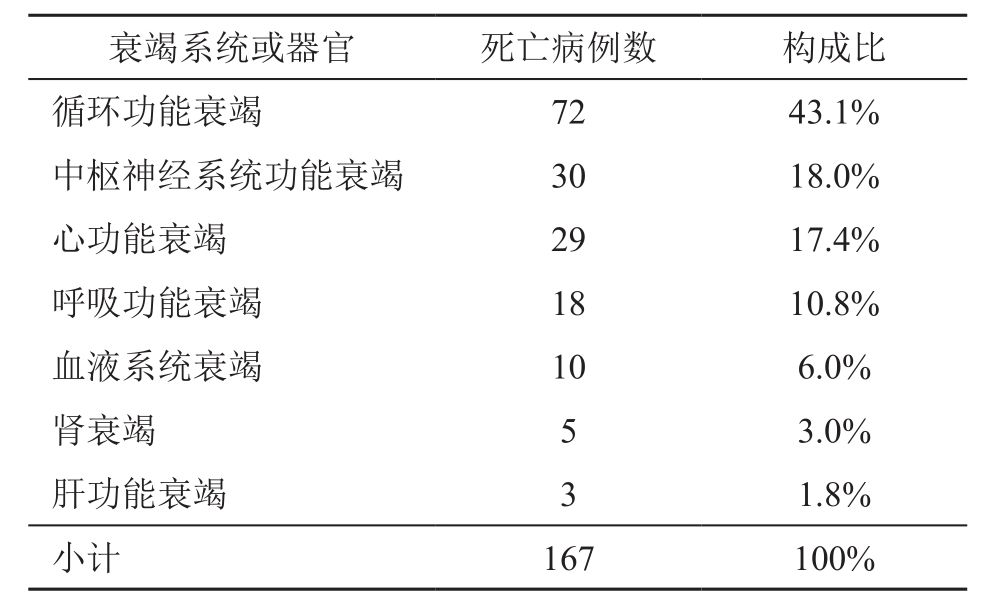
\includegraphics[width=3.35417in,height=2.04167in]{./images/Image00146.jpg}
\end{table}

\protect\hypertarget{text00095.html}{}{}

\section{多器官功能障碍综合征的治疗原则}

所有多器官功能障碍综合征(MODS)患者均应进入重症医学科(ICU),但MODS患者的监测和治疗应由专科医师和ICU专职医师共同完成。尽管MODS的病因复杂、涉及的器官和系统多、治疗中往往面临很多矛盾,但MODS的治疗应遵循以下原则。

\subsubsection{控制原发病}

控制原发疾病是MODS治疗的关键,应重视原发疾病的处理。对于存在严重感染的患者,必须积极的引流感染灶和目标性应用有效抗生素。若为创伤患者,则应积极清创,并预防感染的发生。当重症患者出现腹胀、不能进食或无石性胆囊炎时,应采用积极的措施,如导泻、灌肠等,以保持肠道通畅,恢复肠道屏障功能,避免肠道菌群移位。而对于休克患者,则应争分夺秒的进行休克复苏,尽可能地缩短休克时间,避免引起进一步的器官功能损害。

\subsubsection{改善氧代谢,纠正组织缺氧}

氧代谢障碍是MODS的特征之一,纠正组织缺氧是MODS重要的治疗目标。改善氧代谢障碍、纠正组织缺氧的主要手段包括增加全身氧输送、降低全身氧耗、改善组织细胞利用氧的能力等。

\subparagraph{增加氧输送}

提高氧输送是目前改善组织缺氧最可行的手段。氧输送是单位时间内心脏泵出的血液所携带的氧量,由心脏泵功能、动脉氧分压/血氧饱和度和血红蛋白浓度决定,因此,提高氧输送也就通过心脏、血液和肺交换功能3个方面来实现。

\hypertarget{text00095.htmlux5cux23CHP3-11-4-2-1-1}{}
(1) 维持动脉氧合:

提高动脉氧分压或动脉血氧饱和度是提高全身氧输送的3个基本手段之一。氧疗、呼吸机辅助通气和控制通气是支持动脉氧合的常用手段。

至于支持动脉氧合的目标,不同类型的患者有不同的要求。对于非急性呼吸窘迫综合征或急性呼衰患者,支持动脉氧合的目标是将动脉氧分压维持在80mmHg以上、或动脉血氧饱和度维持在94\%以上。但对于急性呼吸窘迫综合征和急性呼衰患者,将动脉氧分压维持在80mmHg以上常常是困难的,往往需要提高呼吸机条件、增加呼气末正压水平或提高吸入氧浓度,有可能导致气压伤或引起循环干扰,因此,对于这类患者,支持动脉氧合的目标是将动脉氧分压维持在高于55~60mmHg水平以上、或动脉血氧饱和度高于90\%以上。之所以将动脉氧分压维持在55~60mmHg以上,与动脉血氧离曲线的“S”型特征有关,当动脉氧分压高于55~60mmHg水平时,动脉血氧饱和度达到90\%,进一步提高动脉氧分压,呼吸和循环的代价很大,但动脉血氧饱和度增加却并不明显,氧输送也就不会明显增加。

\hypertarget{text00095.htmlux5cux23CHP3-11-4-2-1-2}{}
(2) 维持心输出量:

增加心输出量也是提高全身氧输送的基本手段。保证适当的前负荷、应用正性肌力药物和降低心脏后负荷是支持心输出量的主要方法。

调整前负荷是支持心输出量首先需要考虑的问题,也是最容易处理的环节。若前负荷不足,则可导致心输出量明显降低。而前负荷过高,又可能导致肺水肿和心脏功能降低。因此,调整心脏前负荷具有重要的临床意义。当然,对于重症患者,由于血管张力的改变以及毛细血管通透性的明显增加,往往使患者的有效循环血量明显减少,也就是说,前负荷减少更为常见。监测中心静脉压或肺动脉嵌顿压,可指导前负荷的调整。液体负荷试验后或利尿后,观察肺动脉嵌顿压与心输出量的关系(心功能曲线)的动态变化,比单纯监测压力的绝对值更有价值。补充血容量,可选择晶体液和胶体液,考虑到危重患者毛细血管通透性明显增加,晶体液在血管内的保持时间较短,易转移到组织间隙,应适当提高胶体液的补充比例。

\hypertarget{text00095.htmlux5cux23CHP3-11-4-2-1-3}{}
(3) 增加血液携带氧能力:

维持适当的血红蛋白浓度是改善氧输送的重要手段之一。由于血红蛋白是氧气的载体,机体依赖血红蛋白将氧从肺毛细血管携带到组织毛细血管,维持适当的血红蛋白浓度实际上就是支持血液携带氧能力。但是,并非血红蛋白浓度越高,就对机体越有利。当血红蛋白浓度过高时(如高于14g/dl),血液黏滞度明显增加,不但增加心脏负荷,而且影响血液在毛细血管内的流动,最终影响组织氧合。一般认为,血红蛋白浓度的目标水平是8~10g/dl以上或血细胞比容维持在30\%~35\%左右。

\subparagraph{降低氧耗}

降低氧耗在MODS治疗中常常被忽视。由于组织缺氧是氧供和氧需失衡的结果,氧耗增加也是导致组织缺氧和MODS的原因之一,降低氧耗对MODS的防治具有重要意义。

导致重症患者氧耗增加的因素很多,针对不同原因进行治疗,就成为防治MODS的重要手段。体温每增加1℃,机体氧需增加7\%,氧耗可能增加25\%。因此,及时降温,对于发热的患者就很必要。可采用解热镇痛药物和物理降温等手段。物理降温时,要特别注意防止患者出现寒战。一旦发生寒战,机体氧耗将增加100\%~400\%,对机体的危害很大。疼痛和烦躁也是导致机体氧耗增加的常见原因。有效的镇痛和镇静,使患者处于较为舒适的安静状态,对防止MODS有益。抽搐导致氧耗增加也十分明显,及时止痉是必要的。正常情况下,呼吸肌的氧耗占全身氧耗的1\%~3\%,若患者出现呼吸困难或呼吸窘迫,则呼吸肌的氧耗骤增,呼吸肌的氧需可能增加到占全身氧需的20\%~50\%。呼吸氧需的明显增加,势必造成其他器官的缺氧。采取积极措施,如机械通气或提高机械通气条件,改善患者的呼吸困难,能明显降低患者呼吸肌氧耗。

\subsubsection{代谢支持与调理}

MODS使患者处于高度应激状态,导致机体出现以高分解代谢为特征的代谢紊乱。机体分解代谢明显高于合成代谢,蛋白质分解、脂肪分解和糖异生明显增加,但糖的利用能力明显降低。Cerra将之称为自噬现象(autocannibalism)。严重情况下,机体蛋白质分解代谢较正常增加40\%~50\%,而骨骼肌的分解可增加70\%~110\%,分解产生的氨基酸部分经糖异生作用后供能,部分供肝脏合成急性反应蛋白。器官及组织细胞的功能维护和组织修复有赖于细胞得到适当的营养底物,机体高分解代谢和外源性营养利用障碍,可导致或进一步加重器官功能障碍。因此,在MODS早期,代谢支持和调理的目标应当是试图减轻营养底物不足,防止细胞代谢紊乱,支持器官、组织的结构功能,参与调控免疫功能,减少器官功能障碍的产生。而在MODS的后期,代谢支持和调理的目标是进一步加速组织修复,促进患者康复。

\subparagraph{代谢支持}

代谢支持(metabolic support)是Cerra
1988年提出的,指为机体提供适当的营养底物,以维持细胞代谢的需要,而不是供给较多的营养底物以满足机体营养的需要。与营养支持的区别在于代谢支持既防止因底物供应受限影响器官的代谢和功能,又避免因底物供给量过多而增加器官的负担,影响器官的代谢和功能。其具体实施方法:①非蛋白热卡<
35kcal/(kg•d){[}146kJ/(kg•d){]},一般为25~30kcal/(kg•d),其中40\%~50\%的热卡由脂肪提供,以防止糖代谢紊乱,减少二氧化碳生成,降低肺的负荷。②提高氮的供应量{[}0.25~0.35g/(kg•d){]},以减少体内蛋白质的分解和供给急性反应蛋白合成的需要。③非蛋白热卡与氮的比例降低到100kcal∶1g。

尽管代谢支持的应用,对改善MODS的代谢紊乱有一定的疗效,但并不能避免或逆转代谢紊乱。

\subparagraph{代谢调理}

代谢调理是代谢支持的必要补充。由于MODS患者处于高分解代谢状态,虽根据代谢支持的要求给予营养,仍不能达到代谢支持的目的,机体继续处于高分解代谢状态,供给的营养底物不能维持机体代谢的需要。因此,1989年Shaw提出从降低代谢率或促进蛋白质合成的角度着手,应用药物和生物制剂,以调理机体的代谢,称为代谢调理(metabolic
intervention)。主要方法包括:①应用布洛芬、吲哚美辛等环氧化酶抑制剂,抑制前列腺素合成,降低分解代谢率,减少蛋白质分解;②应用重组的人类生长激素和生长因子,促进蛋白质合成,改善负氮平衡。

代谢调理的应用明显降低了机体分解代谢率,并改善负氮平衡,但代谢调理也不能从根本上逆转高分解代谢和负氮平衡。根据对MODS患者代谢特点,利用代谢支持和代谢调理对机体继续调控和治疗,可望进一步提高营养代谢支持的疗效,改善MODS患者的预后。

\subsubsection{免疫调节治疗}

基于炎症反应失控是导致MODS的本质性原因这一认识,抑制SIRS有可能阻断炎症反应发展,最终可能降低MODS病死率。免疫调控治疗实际上就MODS病因治疗的重要方面。当前,对机体炎症反应认识的深入,取得了阶段性的成果,但要对MODS治疗发挥指导性作用,尚有待时日。

\subparagraph{炎症反应失控的评估和 MODS治疗策略}

正确判断MODS患者SIRS/CARS失衡方向,是进行临床干预、恢复SIRS与CARS平衡的前提。虽然目前尚无快速、准确的指标应用于临床,但有关外周血单核细胞表面HLA-DR表达量及T辅助细胞(TH)\textsubscript{1}
/TH\textsubscript{2} 功能的研究,可判断SIRS/
CARS的失衡方向,从而为指导免疫调控治疗带来曙光。

外周血单核细胞表面HLA-DR表达量是反映细胞免疫功能状态的客观指标之一。Bone提出HLA-DR的表达量低于30\%则可诊断CARS。Kox选择10例严重感染伴MODS的CARS患者,给予IFNγ-lb,结果在3天内全部患者的单核细胞HLA-DR的表达量显著增加,而且释放TNFα和IL-1的能力也明显恢复,提示IFNγ可逆转CARS。当然,HLA-DR表达>
30\%时是否反映机体以SIRS为主,尚难以确定。因此,HLA-DR的表达量仅能粗略反映机体免疫功能状态,尚难以用于评价SIRS/CARS失衡方向。

TH\textsubscript{1} /TH\textsubscript{2}
细胞功能改变也能够反映机体的免疫功能状态,TH\textsubscript{1}
/TH\textsubscript{2}
漂移方向则有助于反映SIRS/CARS的失衡方向和程度。根据TH细胞所分泌的不同淋巴因子及其功能,将TH细胞分为TH\textsubscript{1}
和TH\textsubscript{2} 细胞两种类型,TH\textsubscript{1}
细胞以产生IL-2、IFNγ、TNFβ等促炎介质为特征,增强炎症细胞细胞毒性作用,介导细胞免疫应答。TH\textsubscript{2}
细胞可产生IL-4、IL-5、IL-10、IL-13等细胞因子,以抗炎症反应为主,促进抗体生成,介导体液免疫应答。可见,TH\textsubscript{1}
和TH\textsubscript{2}
细胞实际上分别反映促炎和抗炎反应,两者的失衡则反映了SIRS
和CARS是否失衡,是MODS免疫失衡的重要环节。

感染、创伤时TH\textsubscript{1} 向TH\textsubscript{2}
漂移,说明机体发生细胞免疫功能低下,CARS占优势。此时免疫调控的重点应放在通过促进TH\textsubscript{0}
向TH\textsubscript{1} 分化,同时对PGE\textsubscript{2}
-TH\textsubscript{2}
通道进行下调,重建细胞免疫功能,恢复SIRS和CARS的平衡。Mannick对烧伤动物的研究显示,外源性补充IL-12促进TH\textsubscript{0}
向TH\textsubscript{1}
细胞分化,增强动物的抗感染能力,结果动物病死率显著降低到15\%(对照组为85\%)。Kox应用IFNγlb促进单核细胞分泌IL-6和TNFα,以对抗CARS,而且IFNγ通过抑制单核细胞释放IL-10,阻止PGE\textsubscript{2}
的释放,从而对PGE\textsubscript{2} -TH\textsubscript{2}
通道进行下调。尽管IFNγ等能够有效促进TH\textsubscript{2}
向TH\textsubscript{1}
漂移,但是否能够恢复机体免疫功能,降低MODS患者的病死率,尚有待进一步的临床观察。

\subparagraph{炎症介质基因表达的多态性与 MODS治疗策略}

近年来,分子生物学的发展,尤其是以抑制炎症反应为主的免疫调控治疗临床试验失败,使人们逐渐注意到遗传和基因特征参与感染创伤和MODS的发病过程。研究证实TNF和IL-1等炎症介质基因具有多态性的特点。TNFβ基因上游调控区(启动子区)-308位点含有NcoI限制性内切酶多态性位点。一项对40例严重感染患者的研究表明,具有NcoI限制性内切酶多态性位点的TNFβ\textsubscript{2}
纯合子患者,血浆TNF浓度和患者病死率均显著高于TNFβ\textsubscript{1}
纯合子患者,证实TNFβ\textsubscript{2}
基因型可能是患者释放高浓度TNFα和凶险预后的基因标志。IL-1β基因外显子5具有TaqI限制性内切酶的多态性位点。体外实验显示,含有TaqI多态性位点的IL-1β基因纯合子(A\textsubscript{2}
/A\textsubscript{2}
)患者,单核细胞受LPS刺激后,IL-1β的释放明显增加,但对严重感染的易感性研究则发现IL-1β的TaqI基因多态性与严重感染易感性和病死率无明显相关。

当然,抗炎介质也具有基因多态性的特征。IL-1受体拮抗剂(IL-1ra)基因多态性表现为内含子2中具有不同重复数量的86个bp的重复序列。具有2个重复序列的纯合子IL-1ra
A\textsubscript{2} /A\textsubscript{2}
的患者,IL-1ra的表达量较低,感染易感性高,而且一旦发生严重感染,病死率明显高于其他基因型的患者。可见,IL-1ra基因多态性是IL-1ra表达水平和预后的基因标志。

细胞因子的基因型不同,免疫炎症性反应不同。特别值得注意的是,基因表达的多态性对介质表达、感染易感性和危重患者预后具有明显不同的影响。可见,基因多态性与感染患者炎症反应的差异有关。极富挑战性的是,哪些炎症相关基因具有多态性的特征,目前尚不清楚。炎症相关基因多态性的研究日益受到重视,通过对MODS动物和患者炎症相关基因多态性的分析,试图寻找与感染及MODS的相关基因,弄清细胞因子基因多态性对炎症反应程度和患者预后的影响,并为进一步的基因调控治疗和个体化的免疫调控治疗奠定基础。

总之,全面深刻的认识和研究MODS的发病机制,采用积极合理的干预手段,随着器官支持手段和技术的不断完善,必将提高MODS的抢救成功率。

\protect\hypertarget{text00096.html}{}{}

\hypertarget{text00096.htmlux5cux23CHP3-11-5}{}
参 考 文 献

1. Baue AE. Multiple,progressive,or sequential systems failure:a
syndrome of the 1970s. Arch Surg,1975,110:779-781

2. Tilney NL,Bailey GL,Morgan MD,et al. Sequential system failure of
abdominal aortic aneurysms:an unsolved problem in postoperative care.
Ann Surg,1973,178:117-122

3. Eiseman B,Beart R,Norton L,et al. Multiple organ failure. Surg
Gynecol Obstet,1977,144:323-326

4. Fry DE,Pearlstein L,Fulton RL,et al. Multiple system organ
failure:the role of uncontrolled infection. Arch
Surg,1980,15:136-140

5. Johnson D,Mayers I. Multiple organ dysfunction syndrome:a narrative
review. Can J Anesth,2001,48:502-509

6. Marshall JC. SIRS and MODS:what is their relevance to the science
and practice of intensive care? Shock,2000,14:586-589

7. Deitch EA,Xu D,Kaise VL. Role of the gut in the development of
injury- and shock induced SIRS and MODS:the gutlymph hypothesis,a
review. Front Biosci,2006,11:520-528

8. Knotzer H,Pajk W,Dünser MW,et al. Regional Microvascular Function
and Vascular Reactivity in Patients with Different Degrees of Multiple
Organ Dysfunction Syndrome. Anesth. Analg,2006,102:1187-1193

9. Baue AE. MOF,MODS,and SIRS:what is in a name or an acronym?
Shock,2006,26:438-449

10. Marshall JC. Modeling MODS:what can be learned from animal models
of the multiple-organ dysfunction syndrome?Intensive Care
Med,2005,31:605-608

\protect\hypertarget{text00097.html}{}{}

